\documentclass[twoside]{book}

% Packages required by doxygen
\usepackage{fixltx2e}
\usepackage{calc}
\usepackage{doxygen}
\usepackage[export]{adjustbox} % also loads graphicx
\usepackage{graphicx}
\usepackage[utf8]{inputenc}
\usepackage{makeidx}
\usepackage{multicol}
\usepackage{multirow}
\PassOptionsToPackage{warn}{textcomp}
\usepackage{textcomp}
\usepackage[nointegrals]{wasysym}
\usepackage[table]{xcolor}

% Font selection
\usepackage[T1]{fontenc}
\usepackage[scaled=.90]{helvet}
\usepackage{courier}
\usepackage{amssymb}
\usepackage{sectsty}
\renewcommand{\familydefault}{\sfdefault}
\allsectionsfont{%
  \fontseries{bc}\selectfont%
  \color{darkgray}%
}
\renewcommand{\DoxyLabelFont}{%
  \fontseries{bc}\selectfont%
  \color{darkgray}%
}
\newcommand{\+}{\discretionary{\mbox{\scriptsize$\hookleftarrow$}}{}{}}

% Page & text layout
\usepackage{geometry}
\geometry{%
  a4paper,%
  top=2.5cm,%
  bottom=2.5cm,%
  left=2.5cm,%
  right=2.5cm%
}
\tolerance=750
\hfuzz=15pt
\hbadness=750
\setlength{\emergencystretch}{15pt}
\setlength{\parindent}{0cm}
\setlength{\parskip}{3ex plus 2ex minus 2ex}
\makeatletter
\renewcommand{\paragraph}{%
  \@startsection{paragraph}{4}{0ex}{-1.0ex}{1.0ex}{%
    \normalfont\normalsize\bfseries\SS@parafont%
  }%
}
\renewcommand{\subparagraph}{%
  \@startsection{subparagraph}{5}{0ex}{-1.0ex}{1.0ex}{%
    \normalfont\normalsize\bfseries\SS@subparafont%
  }%
}
\makeatother

% Headers & footers
\usepackage{fancyhdr}
\pagestyle{fancyplain}
\fancyhead[LE]{\fancyplain{}{\bfseries\thepage}}
\fancyhead[CE]{\fancyplain{}{}}
\fancyhead[RE]{\fancyplain{}{\bfseries\leftmark}}
\fancyhead[LO]{\fancyplain{}{\bfseries\rightmark}}
\fancyhead[CO]{\fancyplain{}{}}
\fancyhead[RO]{\fancyplain{}{\bfseries\thepage}}
\fancyfoot[LE]{\fancyplain{}{}}
\fancyfoot[CE]{\fancyplain{}{}}
\fancyfoot[RE]{\fancyplain{}{\bfseries\scriptsize Generated by Doxygen }}
\fancyfoot[LO]{\fancyplain{}{\bfseries\scriptsize Generated by Doxygen }}
\fancyfoot[CO]{\fancyplain{}{}}
\fancyfoot[RO]{\fancyplain{}{}}
\renewcommand{\footrulewidth}{0.4pt}
\renewcommand{\chaptermark}[1]{%
  \markboth{#1}{}%
}
\renewcommand{\sectionmark}[1]{%
  \markright{\thesection\ #1}%
}

% Indices & bibliography
\usepackage{natbib}
\usepackage[titles]{tocloft}
\setcounter{tocdepth}{3}
\setcounter{secnumdepth}{5}
\makeindex

% Hyperlinks (required, but should be loaded last)
\usepackage{ifpdf}
\ifpdf
  \usepackage[pdftex,pagebackref=true]{hyperref}
\else
  \usepackage[ps2pdf,pagebackref=true]{hyperref}
\fi
\hypersetup{%
  colorlinks=true,%
  linkcolor=blue,%
  citecolor=blue,%
  unicode%
}

% Custom commands
\newcommand{\clearemptydoublepage}{%
  \newpage{\pagestyle{empty}\cleardoublepage}%
}

\usepackage{caption}
\captionsetup{labelsep=space,justification=centering,font={bf},singlelinecheck=off,skip=4pt,position=top}

%===== C O N T E N T S =====

\begin{document}

% Titlepage & ToC
\hypersetup{pageanchor=false,
             bookmarksnumbered=true,
             pdfencoding=unicode
            }
\pagenumbering{alph}
\begin{titlepage}
\vspace*{7cm}
\begin{center}%
{\Large Anahita\+Plus }\\
\vspace*{1cm}
{\large Generated by Doxygen 1.8.13}\\
\end{center}
\end{titlepage}
\clearemptydoublepage
\pagenumbering{roman}
\tableofcontents
\clearemptydoublepage
\pagenumbering{arabic}
\hypersetup{pageanchor=true}

%--- Begin generated contents ---
\chapter{coding\+\_\+guidelines}
\label{md_coding_docs_coding_guidelines}
\Hypertarget{md_coding_docs_coding_guidelines}
Use \href{https://akrabat.com/the-beginners-guide-to-contributing-to-a-github-project/}{\texttt{ usual steps}} to make changes into the project just like other Git\+Hub projects.\hypertarget{md_coding_docs_coding_guidelines_autotoc_md0}{}\doxysection{Code style}\label{md_coding_docs_coding_guidelines_autotoc_md0}

\begin{DoxyItemize}
\item {\itshape Cpp} follow R\+OS \href{http://wiki.ros.org/CppStyleGuide}{\texttt{ Cpp Style Guide}} rigorously. ~\newline

\item {\itshape C\+Make} follow Caktin \href{http://docs.ros.org/jade/api/catkin/html/user_guide/standards.html}{\texttt{ C\+Make Style Guide}}. ~\newline

\item {\itshape Python} code should follow \href{http://www.python.org/dev/peps/pep-0008/}{\texttt{ pep8}}. Please see \href{http://wiki.ros.org/PyStyleGuide}{\texttt{ R\+OS Py\+Style\+Guide}} for details. Use {\ttfamily Anaconda} plugin for sublime text editor for style check. ~\newline

\item {\itshape Bash} Use this \href{http://arachnoid.com/python/beautify_bash_program.html}{\texttt{ python script}}. ~\newline

\item {\itshape Roslint} All pkgs (except {\ttfamily commons} pkgs which don\textquotesingle{}t have cpp or py code) depend on \href{http://wiki.ros.org/roslint}{\texttt{ roslint}} for static code analysis. ~\newline

\end{DoxyItemize}

{\bfseries{Note\+:}} \href{https://github.com/AUV-IITK/auv2017/tree/master/utils}{\texttt{ Utils}} contains scripts for formatting {\ttfamily cpp}, {\ttfamily python}, {\ttfamily xml}, {\ttfamily C\+Make\+Lists} files. Since these are bash scripts, there is a formatting script for {\ttfamily bash}.

\DoxyHorRuler{0}
\hypertarget{md_coding_docs_coding_guidelines_autotoc_md1}{}\doxysection{Documentation}\label{md_coding_docs_coding_guidelines_autotoc_md1}
We maintain two forms of online documentation for R\+OS packages\+: ~\newline

\begin{DoxyItemize}
\item {\itshape wiki pages} / External docs\+: This is the A\+U\+V\+Wiki repo. Home for tutorials, design documents and other sorts of information. This is mainly for people running your code. In general anything that people need to know outside source i.\+e. while only running auv code goes in the auv-\/wiki, anything else goes to package doc.
\item {\itshape auto-\/generated code documentation} Internal docs\+: This is mainly for people integrating with or editing your code. There are auto generated from source code comments using doxygen. Travis CI generated and auto deploys to gh-\/pages branch. Located at \href{http://auv-iitk.github.io/auv/}{\texttt{ http\+://auv-\/iitk.\+github.\+io/auv/}} . Look at \href{https://github.com/AUV-IITK/auv/pull/103/commits/c23d7efdadbfd611276e20509f98e6b39328fa20}{\texttt{ sample commit}} to see how to add documentation. Also \href{https://www.stack.nl/~dimitri/doxygen/manual/docblocks.html}{\texttt{ Doxygen manual}} is good for quick start.
\end{DoxyItemize}

\DoxyHorRuler{0}
\hypertarget{md_coding_docs_coding_guidelines_autotoc_md2}{}\doxysection{Source control}\label{md_coding_docs_coding_guidelines_autotoc_md2}
We use Git. Read the wiki page on git.

\DoxyHorRuler{0}
\hypertarget{md_coding_docs_coding_guidelines_autotoc_md3}{}\doxysection{Bug tracking}\label{md_coding_docs_coding_guidelines_autotoc_md3}
We use github issues on auv repo for tracking bugs.

\DoxyHorRuler{0}
 \hypertarget{md_coding_docs_coding_guidelines_autotoc_md4}{}\doxysection{($<$em$>$\+Still missing$<$/em$>$)  Testing}\label{md_coding_docs_coding_guidelines_autotoc_md4}
We use two level of testing\+: ~\newline

\begin{DoxyItemize}
\item Library\+: At the library level, we use standard unit-\/test frameworks. In C++, we use \href{http://wiki.ros.org/gtest}{\texttt{ gtest}}. In Python, we use \href{http://wiki.ros.org/unittest}{\texttt{ unittest}}. ~\newline

\item Message\+: At the message level, we use \href{http://wiki.ros.org/rostest}{\texttt{ rostest}} to set up a system of R\+OS nodes, run a test node, then tear down the system.
\end{DoxyItemize}

R\+OS has established best \href{http://wiki.ros.org/UnitTesting}{\texttt{ practices and policies}} for writing and running tests. ~\newline
 Auv code is structured in layers, with each layer interacting with the other using {\ttfamily actionlib}. For testing each layer separately we use unit tests nodes which are part of the concerning layer itself. ~\newline


\DoxyHorRuler{0}
\hypertarget{md_coding_docs_coding_guidelines_autotoc_md5}{}\doxysection{Standardization}\label{md_coding_docs_coding_guidelines_autotoc_md5}
Code should use R\+OS services, follow guidelines for their use\+: ~\newline
 use \href{http://wiki.ros.org/rosout}{\texttt{ rosout}} for printing messages ~\newline
 uses the R\+OS \href{http://wiki.ros.org/Clock}{\texttt{ Clock}} for time-\/based routines

\DoxyHorRuler{0}
\hypertarget{md_coding_docs_coding_guidelines_autotoc_md6}{}\doxysection{Large data files}\label{md_coding_docs_coding_guidelines_autotoc_md6}
Large files (anything over 1MB, really) often don\textquotesingle{}t belong in the auv repositories, especially if they are just used for tests. These large files affect the time that it takes to checkout the repository.

\DoxyHorRuler{0}
\hypertarget{md_coding_docs_coding_guidelines_autotoc_md7}{}\doxysection{Naming Convention}\label{md_coding_docs_coding_guidelines_autotoc_md7}
Please refer to \href{http://wiki.ros.org/CppStyleGuide\#Naming}{\texttt{ R\+OS Cpp\+Style\+Guide}} and \href{http://wiki.ros.org/ROS/Patterns/Conventions\#Naming_ROS_Resources}{\texttt{ R\+OS Conventions}}.

Avoid using any sort of Hungarian notation on names and \char`\"{}\+\_\+ptr\char`\"{} on pointers.

\tabulinesep=1mm
\begin{longtabu}spread 0pt [c]{*{3}{|X[-1]}|}
\hline
\PBS\centering \cellcolor{\tableheadbgcolor}\textbf{ {\bfseries{Code Element}} }&\PBS\centering \cellcolor{\tableheadbgcolor}\textbf{ {\bfseries{Style}} }&\PBS\centering \cellcolor{\tableheadbgcolor}\textbf{ {\bfseries{Comment}}  }\\\cline{1-3}
\endfirsthead
\hline
\endfoot
\hline
\PBS\centering \cellcolor{\tableheadbgcolor}\textbf{ {\bfseries{Code Element}} }&\PBS\centering \cellcolor{\tableheadbgcolor}\textbf{ {\bfseries{Style}} }&\PBS\centering \cellcolor{\tableheadbgcolor}\textbf{ {\bfseries{Comment}}  }\\\cline{1-3}
\endhead
Namespace &under\+\_\+scored &Differentiate from class names  \\\cline{1-3}
Class name &Camel\+Case &To differentiate from S\+TL types which I\+SO recommends (do not use \char`\"{}\+C\char`\"{} or \char`\"{}\+T\char`\"{} prefixes)  \\\cline{1-3}
Function name &camel\+Case &Lower case start is almost universal except for .Net world  \\\cline{1-3}
Parameters/\+Locals &under\+\_\+scored &Vast majority of standards recommends this because \+\_\+ is more readable to C++ crowd (although not much to Java/.Net crowd)  \\\cline{1-3}
Member variables &under\+\_\+scored\+\_\+with\+\_\+ &The prefix \+\_\+ is heavily discouraged as I\+SO has rules around reserving \+\_\+identifiers, so we recommend suffix instead  \\\cline{1-3}
Enums and its members &Camel\+Case &Most except very old standards agree with this one  \\\cline{1-3}
Globals &g\+\_\+under\+\_\+scored &You shouldn\textquotesingle{}t have these in first place!  \\\cline{1-3}
Constants &U\+P\+P\+E\+R\+\_\+\+C\+A\+SE &Very contentious and we just have to pick one here, unless if is a private constant in class or method, then use naming for Members or Locals  \\\cline{1-3}
File names &Match case of class name in file &Lot of pro and cons either way but this removes inconsistency in auto generated code (important for R\+OS)  \\\cline{1-3}
\end{longtabu}
\hypertarget{md_coding_docs_coding_guidelines_autotoc_md8}{}\doxysubsection{Header Files}\label{md_coding_docs_coding_guidelines_autotoc_md8}
Use a namespace qualified \#ifdef to protect against multiple inclusion\+:


\begin{DoxyCode}{0}
\DoxyCodeLine{\#ifndef msr\_airsim\_MyHeader\_hpp}
\DoxyCodeLine{\#define msr\_airsim\_MyHeader\_hpp}
\DoxyCodeLine{}
\DoxyCodeLine{//-\/-\/your code}
\DoxyCodeLine{}
\DoxyCodeLine{\#endif}
\end{DoxyCode}


The reason we don\textquotesingle{}t use \#pragma once is because it\textquotesingle{}s not supported if same header file exists at multiple places (which might be possible under R\+OS build system!).\hypertarget{md_coding_docs_coding_guidelines_autotoc_md9}{}\doxysubsection{Bracketing}\label{md_coding_docs_coding_guidelines_autotoc_md9}
Inside function or method body place curly bracket on same line. Outside that the Namespace, Class and methods levels use separate line. This is called \href{https://en.wikipedia.org/wiki/Indent_style\#K.26R_style}{\texttt{ K\&R style}} and its variants are widely used in C++ vs other styles which are more popular in other languages. Notice that curlies are not required if you have single statement, but complex statements are easier to keep correct with the braces.


\begin{DoxyCode}{0}
\DoxyCodeLine{int main(int argc, char* argv[])}
\DoxyCodeLine{\{}
\DoxyCodeLine{     while (x == y) \{}
\DoxyCodeLine{        f0();}
\DoxyCodeLine{        if (cont()) \{}
\DoxyCodeLine{            f1();}
\DoxyCodeLine{        \} else \{}
\DoxyCodeLine{            f2();}
\DoxyCodeLine{            f3();}
\DoxyCodeLine{        \}}
\DoxyCodeLine{        if (x > 100)}
\DoxyCodeLine{            break;}
\DoxyCodeLine{    \}}
\DoxyCodeLine{\}}
\end{DoxyCode}
\hypertarget{md_coding_docs_coding_guidelines_autotoc_md10}{}\doxysubsection{Const and References}\label{md_coding_docs_coding_guidelines_autotoc_md10}
Religiously review all non-\/scalar parameters you declare to be candidate for const and references. If you are coming from languages such as C\#/\+Java/\+Python, the most often mistake you would make is to pass parameters by value instead of {\ttfamily const T\&;} Especially most of the strings, vectors and maps you want to pass as {\ttfamily const T\&;} (if they are readonly) or {\ttfamily T\&} (if they are writable). Also add {\ttfamily const} suffix to methods as much as possible.\hypertarget{md_coding_docs_coding_guidelines_autotoc_md11}{}\doxysubsection{Overriding}\label{md_coding_docs_coding_guidelines_autotoc_md11}
When overriding virtual method, use override suffix.\hypertarget{md_coding_docs_coding_guidelines_autotoc_md12}{}\doxysubsection{Pointers}\label{md_coding_docs_coding_guidelines_autotoc_md12}
This is really about memory management. A simulator has much performance cricial code, so we try and avoid overloading the memory manager with lots of calls to new/delete. We also want to avoid too much copying of things on the stack, so we pass things by reference when ever possible. But when the object really needs to live longer than the call stack you often need to allocate that object on the heap, and so you have a pointer. Now, if management of the lifetime of that object is going to be tricky we recommend using \href{https://cppstyle.wordpress.com/c11-smart-pointers/}{\texttt{ C++ 11 smart pointers}}. But smart pointers do have a cost, so don’t use them blindly everywhere. For private code where performance is paramount, raw pointers can be used. Raw pointers are also often needed when interfacing with legacy systems that only accept pointer types, for example, sockets A\+PI. But we try to wrap those legacy interfaces as much as possible and avoid that style of programming from leaking into the larger code base. ~\newline


Religiously check if you can use const everywhere, for example, {\ttfamily const float $\ast$ const xP}. Avoid using prefix or suffix to indicate pointer types in variable names, i.\+e. use {\ttfamily my\+\_\+obj} instead of {\ttfamily myobj\+\_\+ptr} except in cases where it might make sense to differentiate variables better, for example, {\ttfamily int mynum = 5; int$\ast$ mynum\+\_\+ptr = mynum;}\hypertarget{md_coding_docs_coding_guidelines_autotoc_md13}{}\doxysubsection{R\+O\+S Naming Convention}\label{md_coding_docs_coding_guidelines_autotoc_md13}

\begin{DoxyItemize}
\item Topics and nodes should be names keeping in mind the {\ttfamily ros namespace}. For keeping it noob friendly, global names should be assigned to nodes and topics. ~\newline

\item Package folder name should be same as package name. ~\newline

\item Node file name, executable name and ros node name should be same. ~\newline

\item Dynamic Reconfigure cfg files should be related to what it helps configuring. ~\newline

\item Action files should be named after what action or task is done through them. ~\newline

\item Launch files should be named after what state it will launch the nodes in. ~\newline

\end{DoxyItemize}

\DoxyHorRuler{0}
 
\chapter{Contributing}
\label{autotoc_md14}
\Hypertarget{autotoc_md14}

\begin{DoxyItemize}
\item Please read our short and sweet coding guidelines.
\item For big changes such as adding new feature or refactoring, \href{https://github.com/Hyperion-Software/issues}{\tt file an issue first}. We should discuss first!
\item Use \href{https://akrabat.com/the-beginners-guide-to-contributing-to-a-github-project/}{\tt usual steps} to make contributions just like other Git\+Hub projects. If you are not familiar with Git Branch-\/\+Rebase-\/\+Merge workflow, please \href{http://shitalshah.com/p/git-workflow-branch-rebase-squash-merge/}{\tt read this first}.
\end{DoxyItemize}


\begin{DoxyItemize}
\item Rebase your branch frequently with master (once every 2-\/3 days is ideal).
\item Use same style and formatting as rest of code even if it\textquotesingle{}s not your preferred one.
\item Change any documentation that goes with code changes.
\item Do not include OS specific header files.
\item Keep your pull request small, ideally under 10 files. 
\end{DoxyItemize}
\chapter{documentation}
\label{md_coding_docs_documentation}
\Hypertarget{md_coding_docs_documentation}
Doxygen Documentation Generator

Setting Up Doxygen\+:-\/ 1.\+In directory structure, make a document folder in root directory then run the command doxygen -\/g to generate the dconfig file.

2.\+Edit the configuration file to fit the project. The config file contains detailed description of all the fields. However the following are important. I\+N\+P\+UT\+:-\/ Set the directories where doxygen should be looking for files. G\+E\+N\+E\+R\+A\+TE H\+T\+ML\+:-\/ Set this to yes. P\+R\+O\+J\+E\+CT N\+A\+ME\+:-\/ Sets the project name R\+E\+C\+U\+R\+S\+I\+VE\+:-\/ To search the subdirectories recursively

3.\+Comment the code in doxygen format.

If you place comments before functions or variables use /$\ast$$\ast$ comment line1
\begin{DoxyItemize}
\item comment line2
\item comment line3 $\ast$/
\end{DoxyItemize}

If you place comments after functions or variables use /$\ast$$\ast$$<$ comment line1
\begin{DoxyItemize}
\item comment line2
\item comment line3 $\ast$/

@ or \textbackslash{} preceeded text are considered as doxygen commands

Important commands are\+:-\/ 
\end{DoxyItemize}
\chapter{Overview of the Software Stack (Anahita)}
\label{autotoc_md17}
\Hypertarget{autotoc_md17}
Updated\+: 24th December, 2019

This layer is basically concerned with the low-\/level controller of the vehicle. Previously we used a simple P\+ID controller each of the D\+OF of Anahita. This was implemented in a decoupled manner, i.\+e. we ran the controllers independently for each of the axes, and according to what we intend to do, we pass the desired position, and just apply the P\+ID formula. The parameters for P\+ID are tuned during the time of testing the vehicle in the pool.

The current repository contains an implementation of the Cascaded P\+ID Controller, which basically consists of two P\+ID controllers on top of each other, one for position control and one for velocity control. This controller worked well, but since our localisation was heavily dependent on the readings from the D\+VL, the position controller failed to perform well in depths of water less than 1 metre. This controller was implemented w.\+r.\+t positions and velocities in all directions simultaneously (Euclidean distances) in contrast to the previous method.

We intend to study some new techniques in Controls, and implement them in due course of time. They are\+:


\begin{DoxyItemize}
\item {\bfseries Thruster Allocation Matrix}\+: This is implemented in the code, but I doubt whether it works correctly. Need to check and fix this.
\item {\bfseries L\+QR controller}\+: Used by some teams coming to Robosub, performs well according to them
\item {\bfseries Reinforcement Learning based Controller}\+: This would be very advanced, we\textquotesingle{}ll need to setup a simulation environment with A\+P\+Is according to the RL literature.
\end{DoxyItemize}

This layer was mostly written considering the D\+VL in mind. The Doppler Velocity Log provides us with the velocity information of the water profile near the vehicle. Using that along with the I\+MU, we have created a basic structure for odometry for Anahita. Odometry message tell us about the state of the vehicle in the pool, and is therefore necessary for navigation.

The mapping package is untested. We wrote down the code for an implementation of the Fast\+S\+L\+AM paper, which is basically a landmark-\/based S\+L\+AM. S\+L\+AM stands for Simultaneous Localisation and Mapping, which is the process by which a robot creates a map for the obstacles and landmarks around itself, and further localises itself in the map, by estimating a position with the concerned error in the position.


\begin{DoxyItemize}
\item {\bfseries Vehicle Dynamics Model}\+: We are currently looking at methods concerning Vehicle Dynamic Model based localisation. This would incorporate the dynamics of our vehicle while estimating its position.
\item {\bfseries Visual S\+L\+AM}\+: This is something we are going to implement surely over the next semester. In this, features on images such as corners are located and the change in their positions are processed to calculate your change in state. O\+RB S\+L\+AM is a well-\/known implementation of this technique.
\item {\bfseries Disparity Map Generation}\+: With the procurement of new i\+DS cameras, we hope to setup a stereo mapping system, which would allow us to get depth maps, and find how far the objects are from the vehicle.
\end{DoxyItemize}

This layer basically works as the highest most-\/layer authority for autonomy. Previously, we have used a complex set of {\ttfamily if-\/else} statements combined with timeouts to create this system. This is the basis of intelligent behaviour for the vehicle, and has scope for the most drastic change in all of the stack.


\begin{DoxyItemize}
\item {\bfseries S\+M\+A\+CH}\+: This is a general-\/purpose library for creating heirarichal state machines, where each behaviour is a state, and we have to code the transitions between them.
\item {\bfseries Behaviour Trees}\+: Bascially this is a system of trees, where we would setup a non-\/binary tree-\/like structure for performing tasks.
\item {\bfseries End-\/\+To-\/\+End Deep Reinforcement Learning for Task Completion}
\end{DoxyItemize}

Pretty simple to explain, but one of the toughest challenges lie here. Multiple hardware driver packages are present here, such as\+: {\itshape I\+MU, Cameras, D\+VL, Arduino}.


\begin{DoxyItemize}
\item {\bfseries Hydrophones}\+: Currently we use a Virtual Machine for running the Lab\+View software on our Ubuntu system. This is very unreliable, and has not been tested for longer durations. We need to reverse-\/engineer drivers made available for other Linux-\/distros and configure them to obtain data from the NI D\+AQ board directly to our system. Pure brainstorming and hacking stuff here.
\item {\bfseries i\+DS Cameras}\+: Would be pretty easy to implement depending upon the support for the cameras available online.
\end{DoxyItemize}

Currently has a pre-\/processing timeline implemented (Fusion Framework). Open\+CV nodes for most tasks have been written following a object-\/oriented structure for changing the current tasks. Along with this, a machine-\/learning based approach is also implemented. We have trained Y\+O\+LO with the data collected from the swimming pool and tested it on the Jetson T\+X2.


\begin{DoxyItemize}
\item {\bfseries Tracking and Filtering}\+: Would implement tracking for all the tasks and better filtering of random values during object detection
\item {\bfseries C\+N\+Ns and Style Transfer for Data Generation}\+: Basically work on the computer vision part of the vision team.
\end{DoxyItemize}

Mostly used in the competition and testing time.


\begin{DoxyItemize}
\item {\bfseries G\+UI}\+: We have developed a basic version of the G\+UI, which works on the local network using {\ttfamily ros-\/bridge}. We need to extend this to have more functionality.
\item {\bfseries Color Calibration}\+: Using static values for thresholding makes it suspectible to changing brightness in the pool, and color variations. We need to setup a very abstracted and simplified method for doing this. 
\end{DoxyItemize}
\chapter{Graphical User Interface for Anahita}
\label{autotoc_md25}
\Hypertarget{autotoc_md25}
{\bfseries Clone} the repostitory

To begin, we will launch R\+OS. To do so, run the following in a terminal\+: {\ttfamily roscore}

Then launch the rosbridge v2.\+0 server with the following\+: {\ttfamily roslaunch rosbridge\+\_\+server rosbridge\+\_\+websocket.\+launch}

You should also launch the mmpeg server for video streaming\+: {\ttfamily rosrun web\+\_\+video\+\_\+server ..} 
\chapter{hardware\+\_\+arduino}
\label{autotoc_md28}
\Hypertarget{autotoc_md28}
This is a R\+OS package for interacting arduino through the \href{http://wiki.ros.org/rosserial_arduino}{\tt rosserial\+\_\+arduino} package. The package is meant to actuate thrusters connected to the arduino through a motor driver, and publish the measurements taken from various sensors connected to the arduino onto separate topics.

The {\ttfamily hardware\+\_\+arduino} package has been tested under \href{http://www.ros.org}{\tt R\+OS} Kinetic and Ubuntu 16.\+04 L\+TS. The source code is released under a B\+SD 3-\/\+Clause license.

The hardware used are as follows\+:
\begin{DoxyItemize}
\item \href{https://store.arduino.cc/usa/arduino-mega-2560-rev3}{\tt Arduino M\+E\+GA}
\item \href{http://www.nex-robotics.com/products/motor-drivers/8v-28v-5amp-dual-dc-motor-driver-with-current-sense.html}{\tt 8\+V-\/28V, 5\+Amp Dual DC Motor Driver with Current Sensor}
\item \href{https://www.bluerobotics.com/store/electronics/bar30-sensor-r1/}{\tt Pressure Sensor}
\end{DoxyItemize}


\begin{DoxyItemize}
\item \href{http://wiki.ros.org}{\tt Robot Operating System (R\+OS)} (middleware for robotics),
\item Following R\+OS Packages\+: \href{http://wiki.ros.org/rosserial}{\tt rosserial}, \href{http://wiki.ros.org/rosserial_arduino}{\tt rosserial\+\_\+arduino}
\end{DoxyItemize}

Run the following command to copy the udev rules specified for the Arduino port\+: 
\begin{DoxyCode}
cd ~/catkin\_ws/src/auv2018/utils
sudo bash clone\_udev.sh
\end{DoxyCode}


{\bfseries N\+O\+TE\+:} This connects the arduino always to the port named {\ttfamily /dev/arduino}.

Arduino will likely connect to computer as port {\ttfamily /dev/arduino}. The easiest way to make the determination is to unplug all other U\+SB devices, plug in your Arduino, then run the command\+: 
\begin{DoxyCode}
ls /dev*
\end{DoxyCode}


Next make sure you have read/write access to the port. Assuming your Arduino is connected on {\ttfamily /dev/arduino}, run the command\+:


\begin{DoxyCode}
ls -l /dev/arduino
\end{DoxyCode}
 You should see an output similar to the following\+: 
\begin{DoxyCode}
crw-rw---- 1 root dialout 166, 0 2018-03-05 08:31 /dev/arduino
\end{DoxyCode}


Note that only root and the \char`\"{}dialout\char`\"{} group have read/write access. Therefore, you need to be a member of the dialout group. You only have to do this once and it should then work for all U\+SB devices you plug in later on.

To add yourself to the dialout group, run the command\+: 
\begin{DoxyCode}
sudo usermod -a -G dialout your\_user\_name
\end{DoxyCode}
 where {\ttfamily your\+\_\+user\+\_\+name} is your Linux login name. You will likely have to log out of your X-\/window session then log in again, or simply reboot your machine if you want to be sure.

When you log back in again, try the command\+: 
\begin{DoxyCode}
groups
\end{DoxyCode}
 and you should see a list of groups you belong to including dialout.

Run the following command\+: 
\begin{DoxyCode}
cd ~/catkin\_ws
catkin\_make --pkg hardware\_arduino
\end{DoxyCode}


Run the following command\+: 
\begin{DoxyCode}
cd ~/catkin\_ws
source devel/setup.zsh
catkin\_make hardware\_arduino\_firmware\_arduino\_node    
catkin\_make hardware\_arduino\_firmware\_arduino\_node-upload     
\end{DoxyCode}



\begin{DoxyCode}
        FRONT
        -----
        SWAY1
        HEAVE1
          -
SURGE1           SURGE2
          -
        HEAVE2
        SWAY2
        -----
        BACK
\end{DoxyCode}


For technical definition of terms, refer to documentation \href{https://en.wikipedia.org/wiki/Ship_motions}{\tt here}.

To connect to the arduino, run\+: 
\begin{DoxyCode}
roslaunch hardware\_arduino hardware\_arduino.launch
\end{DoxyCode}
 First upload the code on arduino through Arduino I\+DE.

Subscribes to topics with P\+WM data and actuate the thrusters with that duty cycle, and also publishes the data obtained from pressure sensor

{\bfseries N\+O\+TE\+:} Pins configurations are specified in the \href{include/ArduinoConfig.h}{\tt Arduino\+Config.\+h} file.


\begin{DoxyItemize}
\item $\ast$$\ast${\ttfamily /thruster/surge1/pwm}$\ast$$\ast$ (\href{http://docs.ros.org/api/std_msgs/html/msg/Int32.html}{\tt std\+\_\+msgs/\+Int32})
\item $\ast$$\ast${\ttfamily /thruster/surge2/pwm}$\ast$$\ast$ (\href{http://docs.ros.org/api/std_msgs/html/msg/Int32.html}{\tt std\+\_\+msgs/\+Int32})
\item $\ast$$\ast${\ttfamily /thruster/heave1/pwm}$\ast$$\ast$ (\href{http://docs.ros.org/api/std_msgs/html/msg/Int32.html}{\tt std\+\_\+msgs/\+Int32})
\item $\ast$$\ast${\ttfamily /thruster/heave2/pwm}$\ast$$\ast$ (\href{http://docs.ros.org/api/std_msgs/html/msg/Int32.html}{\tt std\+\_\+msgs/\+Int32})
\item $\ast$$\ast${\ttfamily /thruster/sway1/pwm}$\ast$$\ast$ (\href{http://docs.ros.org/api/std_msgs/html/msg/Int32.html}{\tt std\+\_\+msgs/\+Int32})
\item $\ast$$\ast${\ttfamily /thruster/sway1/pwm}$\ast$$\ast$ (\href{http://docs.ros.org/api/std_msgs/html/msg/Int32.html}{\tt std\+\_\+msgs/\+Int32})
\end{DoxyItemize}


\begin{DoxyItemize}
\item $\ast$$\ast${\ttfamily /pressure\+\_\+sensor/pressure}$\ast$$\ast$ (\href{http://docs.ros.org/hydro/api/underwater_sensor_msgs/html/msg/Pressure.html}{\tt underwater\+\_\+sensor\+\_\+msgs/\+Pressure})\+: Pressure sensor data (in Pascals)
\end{DoxyItemize}

Please report bugs and request features using the \href{https://github.com/AUV-IITK/auv2017/issues}{\tt Issue Tracker}. 
\chapter{hardware\+\_\+camera}
\label{autotoc_md43}
\Hypertarget{autotoc_md43}
This is a R\+OS package for getting feed from the camera using \href{http://wiki.ros.org/usb_cam}{\tt usb\+\_\+cam} and publishing it as a \href{http://docs.ros.org/api/sensor_msgs/html/msg/Image.html}{\tt sensor\+\_\+msgs/\+Image} to the other layers.

The {\ttfamily hardware\+\_\+camera} package has been tested under \href{http://www.ros.org}{\tt R\+OS} Kinetic and Ubuntu 16.\+04 L\+TS. The source code is released under a B\+SD 3-\/\+Clause license.

The hardware used are as follows\+:
\begin{DoxyItemize}
\item Front-\/facing Camera\+: \href{https://www.logitech.com/en-in/product/c930e-webcam}{\tt Logitech C930e}
\item Bottom-\/facing Camera\+: \href{https://www.logitech.com/en-in/product/c930e-webcam}{\tt Logitech C930e}
\end{DoxyItemize}


\begin{DoxyItemize}
\item \href{http://wiki.ros.org}{\tt Robot Operating System (R\+OS)} (middleware for robotics),
\item Following R\+OS Packages\+: \href{http://wiki.ros.org/usb_cam}{\tt usb\+\_\+cam}
\end{DoxyItemize}

The udev rules for the cameras connected to the robot are present in the \mbox{[}/utils/udev\mbox{]} directory. To copy them to your system, run\+: 
\begin{DoxyCode}
cd ~/catkin\_ws/src/auv2018/utils
sudo bash clone\_udev.sh
\end{DoxyCode}


Camera will then be connected to the ports with id {\ttfamily /dev/front\+\_\+cam} and {\ttfamily /dev/bottom\+\_\+cam}.

Run the following command\+: 
\begin{DoxyCode}
cd ~/catkin\_ws
catkin\_make --pkg hardware\_camera
\end{DoxyCode}


To initialize the cmaera nodes, run\+: 
\begin{DoxyCode}
roslaunch hardware\_camera camera\_logitech.launch
\end{DoxyCode}


The {\ttfamily usb\+\_\+cam\+\_\+node} interfaces with standard U\+SB cameras (e.\+g. the Logitech Quickcam) using libusb\+\_\+cam and publishes images as {\ttfamily sensor\+\_\+msgs\+::\+Image}. The node belongs to the \href{http://wiki.ros.org/usb_cam}{\tt usb\+\_\+cam} package.


\begin{DoxyItemize}
\item $\ast$$\ast${\ttfamily hardware\+\_\+camera/front\+\_\+cam/image\+\_\+raw}$\ast$$\ast$ (\href{http://docs.ros.org/api/sensor_msgs/html/msg/Image.html}{\tt sensor\+\_\+msgs/\+Image})
\end{DoxyItemize}


\begin{DoxyItemize}
\item {\ttfamily $\sim$image\+\_\+width} (integer, default\+: 1280) Image width
\item {\ttfamily $\sim$image\+\_\+height} (integer, default\+: 720) Image height
\item {\ttfamily $\sim$framerate} (integer, default\+: 30) The required framerate
\item {\ttfamily $\sim$camera\+\_\+info\+\_\+url} (string, default\+: ) An url to the camera calibration file that will be read by the \href{http://wiki.ros.org/CameraInfoManager}{\tt Camera\+Info\+Manager} class
\end{DoxyItemize}

The {\ttfamily usb\+\_\+cam\+\_\+node} interfaces with standard U\+SB cameras (e.\+g. the Logitech Quickcam) using libusb\+\_\+cam and publishes images as {\ttfamily sensor\+\_\+msgs\+::\+Image}. The node belongs to the \href{http://wiki.ros.org/usb_cam}{\tt usb\+\_\+cam} package.


\begin{DoxyItemize}
\item $\ast$$\ast${\ttfamily bottom\+\_\+camera/image\+\_\+raw}$\ast$$\ast$ (\href{http://docs.ros.org/api/sensor_msgs/html/msg/Image.html}{\tt sensor\+\_\+msgs/\+Image})
\end{DoxyItemize}


\begin{DoxyItemize}
\item {\ttfamily $\sim$image\+\_\+width} (integer, default\+: 1280) Image width
\item {\ttfamily $\sim$image\+\_\+height} (integer, default\+: 720) Image height
\item {\ttfamily $\sim$framerate} (integer, default\+: 30) The required framerate
\item {\ttfamily $\sim$camera\+\_\+info\+\_\+url} (string, default\+: ) An url to the camera calibration file that will be read by the \href{http://wiki.ros.org/CameraInfoManager}{\tt Camera\+Info\+Manager} class.
\end{DoxyItemize}

Please report bugs and request features using the \href{https://github.com/AUV-IITK/auv2018/issues}{\tt Issue Tracker}. 
\chapter{hardware\+\_\+dvl}
\label{autotoc_md58}
\Hypertarget{autotoc_md58}
This is a R\+OS package for interfacing with the Teledyne Pathnfider Doppler Velocity Log hardware

The {\ttfamily hardware\+\_\+dvl} package has been tested under \href{http://www.ros.org}{\tt R\+OS} Kinetic and Ubuntu 16.\+04 L\+TS. The source code is released under a B\+SD 3-\/\+Clause license. 
\chapter{hardware\+\_\+imu}
\label{autotoc_md60}
\Hypertarget{autotoc_md60}
This is a R\+OS package for interfacing with the \href{http://px4.io/}{\tt P\+X4} hardware or the \href{https://www.spartonnavex.com/product/ahrs-8/}{\tt Sparton A\+H\+R\+S-\/8} hardware.

For the P\+X4, we are using the in-\/built inertial measurement unit (I\+MU) present in the P\+X4 for the robot. For the Sparton A\+H\+R\+S8, the driver communicates with the sensor using N\+M\+EA protocol and publishes the I\+MU data as R\+OS sensor messages.

The {\ttfamily hardware\+\_\+imu} package has been tested under \href{http://www.ros.org}{\tt R\+OS} Kinetic and Ubuntu 16.\+04 L\+TS. The source code is released under a B\+SD 3-\/\+Clause license.


\begin{DoxyItemize}
\item \href{http://wiki.ros.org}{\tt Robot Operating System (R\+OS)} (middleware for robotics),
\item Following R\+OS Packages\+: \href{http://wiki.ros.org/mavros}{\tt mavros}, \href{http://wiki.ros.org/mavros_extras}{\tt mavros\+\_\+extras}
\end{DoxyItemize}

According to the installation instructions present \href{https://github.com/mavlink/mavros/blob/master/mavros/README.md#binary-installation-deb}{\tt here}, run the following commands to install Geographic\+Lib datasets which is required as a mavros dependency\+: 
\begin{DoxyCode}
wget
       https://raw.githubusercontent.com/mavlink/mavros/master/mavros/scripts/install\_geographiclib\_datasets.sh
./install\_geographiclib\_datasets.sh
\end{DoxyCode}


Download \href{https://docs.qgroundcontrol.com/en/getting_started/download_and_install.html}{\tt Q\+Ground Control} and run it with P\+I\+X\+H\+A\+WK attached with your computer. Read the manual \href{https://docs.qgroundcontrol.com/en/SetupView/Sensors.html}{\tt here} for further instructions.

Run the following command from the root of your catkin workspace\+: 
\begin{DoxyCode}
catkin\_make --pkg hardware\_imu
\end{DoxyCode}


To run the {\bfseries P\+I\+X\+H\+A\+WK I\+MU}\+: 
\begin{DoxyCode}
roslaunch hardware\_imu imu\_px4.launch
\end{DoxyCode}
 where the P\+I\+X\+H\+A\+WK is assumed to be connected at the {\ttfamily /dev/tty\+A\+C\+M0} port.

To run the {\bfseries Sparton A\+H\+R\+S8 I\+MU}\+:


\begin{DoxyEnumerate}
\item Check the serial port to which the sensor is connected at and change the device path in the \href{launch/ahrs-8.launch}{\tt launch file} 
\begin{DoxyCode}
# to verify if device is at /dev/ttyUSB0, run:
udevadm info -a -p  $(udevadm info -q path -n /dev/ttyUSB0)
\end{DoxyCode}

\item Ensure that python cript has executable permission\+: 
\begin{DoxyCode}
chmod +x sparton\_ahrs8\_driver/scripts/ahrs8\_nmea.py
\end{DoxyCode}

\item Run the launch file\+: 
\begin{DoxyCode}
roslaunch sparton\_ahrs8\_driver ahrs-8.launch
\end{DoxyCode}

\end{DoxyEnumerate}

The {\ttfamily mavros\+\_\+node} is the main communication node for the M\+A\+V\+Link communication protocol used in the P\+X4 autopilot. The node belongs to the \href{http://wiki.ros.org/mavros}{\tt mavros} package.


\begin{DoxyItemize}
\item $\ast$$\ast${\ttfamily $\sim$imu/data}$\ast$$\ast$ (\href{http://docs.ros.org/api/sensor_msgs/html/msg/Imu.html}{\tt sensor\+\_\+msgs/\+Imu}) Imu data, orientation computed by F\+CU
\item $\ast$$\ast${\ttfamily $\sim$imu/data\+\_\+raw}$\ast$$\ast$ (\href{http://docs.ros.org/api/sensor_msgs/html/msg/Imu.html}{\tt sensor\+\_\+msgs/\+Imu}) Raw I\+MU data without orientation
\item $\ast$$\ast${\ttfamily $\sim$imu/mag}$\ast$$\ast$ (\href{http://docs.ros.org/api/sensor_msgs/html/msg/MagneticField.html}{\tt sensor\+\_\+msgs/\+Magnetic\+Field}) F\+CU compass data
\item $\ast$$\ast${\ttfamily $\sim$imu/temperature}$\ast$$\ast$ (\href{http://docs.ros.org/api/sensor_msgs/html/msg/Temperature.html}{\tt sensor\+\_\+msgs/\+Temperature}) Temperature reported by F\+CU (usually from barometer)
\item $\ast$$\ast${\ttfamily $\sim$imu/atm\+\_\+pressure}$\ast$$\ast$ (\href{http://docs.ros.org/api/sensor_msgs/html/msg/FluidPressure.html}{\tt sensor\+\_\+msgs/\+Fluid\+Pressure}) Air pressure.
\end{DoxyItemize}


\begin{DoxyItemize}
\item $\ast$$\ast${\ttfamily $\sim$imu/frame\+\_\+id}$\ast$$\ast$ (string, default\+: fcu) Frame ID for this plugin.
\item $\ast$$\ast${\ttfamily $\sim$imu/linear\+\_\+acceleration\+\_\+stdev}$\ast$$\ast$ (double, default\+: 0.\+0003) Gyro\textquotesingle{}s standard deviation
\item $\ast$$\ast${\ttfamily $\sim$imu/angular\+\_\+velocity\+\_\+stdev}$\ast$$\ast$ (double, default\+: !dec 0.\+02) Accel\textquotesingle{}s standard deviation
\item $\ast$$\ast${\ttfamily $\sim$imu/orientation\+\_\+stdev}$\ast$$\ast$ (double, default\+: 1.\+0) Standard deviation for I\+M\+U.\+orientation
\item $\ast$$\ast${\ttfamily $\sim$imu/magnetic\+\_\+stdev}$\ast$$\ast$ (double, default\+: 0.\+0) Standard deviation for magnetic field message (undefined if\+: 0.\+0)
\end{DoxyItemize}

This node takes the I\+MU data in quateranion format and convert it into euler angles. We calculate the roll, pitch and yaw using the following formulas\+:


\begin{DoxyCode}
yaw = atan2 ( 2 * x * y - 2 * w * z, 2 * w * w + 2 * x * x - 1)
roll = atan2(2 * q2 * q3 - 2 * q0 * q1, 2 * q0 * q0 + 2 * q3 * q3 - 1)
pitch = -asin(2 * q1 * q3 + 2 * q0 * q2)
\end{DoxyCode}
 where {\ttfamily q = (w, x, y, z)} is the quaternion angle.


\begin{DoxyItemize}
\item $\ast$$\ast${\ttfamily $\sim$/mavros/imu/data}$\ast$$\ast$ (\href{http://docs.ros.org/api/sensor_msgs/html/msg/Imu.html}{\tt sensor\+\_\+msgs/\+Imu}) Imu data, orientation computed by F\+CU
\end{DoxyItemize}


\begin{DoxyItemize}
\item $\ast$$\ast${\ttfamily /mavros/imu/yaw}$\ast$$\ast$ (\href{http://docs.ros.org/lunar/api/std_msgs/html/msg/Float64.html}{\tt std\+\_\+msgs/\+Float64}) Yaw data computed using quaternion to euler angles transformation $\ast$$\ast${\ttfamily /mavros/imu/pitch}$\ast$$\ast$ (\href{http://docs.ros.org/lunar/api/std_msgs/html/msg/Float64.html}{\tt std\+\_\+msgs/\+Float64}) Pitch data computed using quaternion to euler angles transformation $\ast$$\ast${\ttfamily /mavros/imu/roll}$\ast$$\ast$ (\href{http://docs.ros.org/lunar/api/std_msgs/html/msg/Float64.html}{\tt std\+\_\+msgs/\+Float64}) Roll data computed using quaternion to euler angles transformation
\end{DoxyItemize}

The node communicate with the sensor using the N\+M\+EA protocol and publishes I\+MU data.


\begin{DoxyItemize}
\item $\ast$$\ast${\ttfamily $\sim$frame\+\_\+id}$\ast$$\ast$ (string, default\+: {\ttfamily ahrs8\+\_\+imu}) Frame ID for this plugin
\item $\ast$$\ast${\ttfamily $\sim$port}$\ast$$\ast$ (string, default\+: {\ttfamily /dev/tty\+U\+S\+B0}) Port at which sensor is connected
\item $\ast$$\ast${\ttfamily $\sim$baud}$\ast$$\ast$ (double, default\+: {\ttfamily 115200}) Baud rate for communication with the sensor
\end{DoxyItemize}


\begin{DoxyItemize}
\item $\ast$$\ast${\ttfamily $\sim$imu/data}$\ast$$\ast$ (\href{http://docs.ros.org/api/sensor_msgs/html/msg/Imu.html}{\tt sensor\+\_\+msgs/\+Imu}) I\+MU orientation data, orientation in the {\ttfamily ahrs8\+\_\+imu} frame
\end{DoxyItemize}

This node takes the I\+MU data in quateranion format and convert it into euler angles. We calculate the roll, pitch and yaw using the above formulas again


\begin{DoxyItemize}
\item $\ast$$\ast${\ttfamily $\sim$/sparton/imu/data}$\ast$$\ast$ (\href{http://docs.ros.org/api/sensor_msgs/html/msg/Imu.html}{\tt sensor\+\_\+msgs/\+Imu}) Imu data, orientation computed by F\+CU
\end{DoxyItemize}


\begin{DoxyItemize}
\item $\ast$$\ast${\ttfamily /sparton/imu/yaw}$\ast$$\ast$ (\href{http://docs.ros.org/lunar/api/std_msgs/html/msg/Float64.html}{\tt std\+\_\+msgs/\+Float64}) Yaw data computed using quaternion to euler angles transformation $\ast$$\ast${\ttfamily /sparton/imu/pitch}$\ast$$\ast$ (\href{http://docs.ros.org/lunar/api/std_msgs/html/msg/Float64.html}{\tt std\+\_\+msgs/\+Float64}) Pitch data computed using quaternion to euler angles transformation $\ast$$\ast${\ttfamily /sparton/imu/roll}$\ast$$\ast$ (\href{http://docs.ros.org/lunar/api/std_msgs/html/msg/Float64.html}{\tt std\+\_\+msgs/\+Float64}) Roll data computed using quaternion to euler angles transformation
\end{DoxyItemize}

Please report bugs and request features using the \href{https://github.com/AUV-IITK/fourtran/issues}{\tt Issue Tracker}. 
\chapter{Teledyne Navigator R\+OS Package}
\label{autotoc_md81}
\Hypertarget{autotoc_md81}
\href{https://dev.mcgillrobotics.com/job/ros-teledyne-navigator/job/master}{\tt !\mbox{[}status\mbox{]}}

This R\+OS package configures and communicates with the Teledyne Navigator Doppler Velocity Log (D\+VL). {\bfseries This has only been tested on R\+OS Kinetic and Melodic over R\+S232.}

You must clone this repository as {\ttfamily teledyne\+\_\+navigator} into your {\ttfamily catkin} workspace\textquotesingle{}s {\ttfamily src} directory\+:


\begin{DoxyCode}
roscd
cd src
git clone https://github.com/mcgill-robotics/ros-teledyne-navigator.git teledyne\_navigator
\end{DoxyCode}


Before proceeding, make sure to install all the dependencies by running\+:


\begin{DoxyCode}
rosdep update
rosdep install teledyne\_navigator
\end{DoxyCode}


You {\bfseries must} compile this package before being able to run it. You can do so by running\+:


\begin{DoxyCode}
catkin\_make
\end{DoxyCode}


from the root of your workspace.

To run, simply connect the D\+VL over R\+S232 and launch the package with\+:


\begin{DoxyCode}
roslaunch teledyne\_navigator teledyne\_navigator.launch port:=</path/to/dvl>
\end{DoxyCode}


The following run-\/time R\+OS launch arguments are available\+:


\begin{DoxyItemize}
\item {\ttfamily port}\+: Serial port to read from, default\+: {\ttfamily /dev/dvl}.
\item {\ttfamily baudrate}\+: Serial baud rate, default\+: {\ttfamily 9600}.
\item {\ttfamily timeout}\+: Serial read timeout in seconds, default\+: {\ttfamily 1.\+0}.
\item {\ttfamily frame}\+: {\ttfamily tf} frame to stamp the messages with, default\+: {\ttfamily dvl}.
\end{DoxyItemize}

The package will keep trying to connect to the D\+VL until it is successful.

The {\ttfamily teledyne\+\_\+navigator} node will output to the following R\+OS topic\+:


\begin{DoxyItemize}
\item {\ttfamily $\sim$ensemble}\+: D\+VL scan data as an {\ttfamily Ensemble} message.
\end{DoxyItemize}

This driver is limited to the P\+D5 output format and the earth-\/coordinate frame (E\+NU). You may change other parameters as you please using T\+R\+DI Toolz and save them with {\ttfamily CK}, but the {\ttfamily PD} and {\ttfamily EX} commands will be overridden.

Contributions are welcome. Simply open an issue or pull request on the matter, and it will be accepted as long as it does not complicate the code base too much.

As for style guides, we follow the R\+OS Python Style Guide for R\+O\+S-\/specifics and the Google Python Style Guide for everything else.

We use \href{https://github.com/google/yapf}{\tt Y\+A\+PF} for all Python formatting needs. You can auto-\/format your changes with the following command\+:


\begin{DoxyCode}
yapf --recursive --in-place --parallel .
\end{DoxyCode}


We also use \href{https://github.com/fkie/catkin_lint}{\tt catkin\+\_\+lint} for all {\ttfamily catkin} specifics. You can lint your changes as follows\+:


\begin{DoxyCode}
catkin lint --explain -W2 .
\end{DoxyCode}


See \mbox{[}L\+I\+C\+E\+N\+SE\mbox{]}(L\+I\+C\+E\+N\+SE). 
\chapter{A\+UV Anahita}
\label{autotoc_md90}
\Hypertarget{autotoc_md90}
This repository contains the code for our second underwater vehicle {\ttfamily Anahita}.

\tabulinesep=1mm
\begin{longtabu} spread 0pt [c]{*{4}{|X[-1]}|}
\hline
\rowcolor{\tableheadbgcolor}\PBS\centering \textbf{ S. No. }&\PBS\centering \textbf{ Operating System }&\PBS\centering \textbf{ R\+OS Version }&\PBS\centering \textbf{ Build Status  }\\\cline{1-4}
\endfirsthead
\hline
\endfoot
\hline
\rowcolor{\tableheadbgcolor}\PBS\centering \textbf{ S. No. }&\PBS\centering \textbf{ Operating System }&\PBS\centering \textbf{ R\+OS Version }&\PBS\centering \textbf{ Build Status  }\\\cline{1-4}
\endhead
\PBS\centering 1. &\PBS\centering \href{http://releases.ubuntu.com/18.04/}{\tt Ubuntu 18.\+04 L\+TS} &\PBS\centering \href{http://wiki.ros.org/Melodic}{\tt Melodic Morenia} &\PBS\centering \href{https://travis-ci.org/AUV-IITK/Anahita}{\tt } \\\cline{1-4}
\end{longtabu}



\begin{DoxyEnumerate}
\item {\bfseries Create a catkin worspace following the guidelines given \href{http://wiki.ros.org/catkin/Tutorials/create_a_workspace}{\tt here}} 
\begin{DoxyCode}
mkdir -p ~/catkin\_ws/src
cd ~/catkin\_ws/src
catkin\_init\_workspace
cd ..
catkin\_make
\end{DoxyCode}

\item {\bfseries Clone this repository to your catkin workspace} 
\begin{DoxyCode}
cd ~/catkin\_ws/src
git clone https://github.com/AUV-IITK/AnahitaPlus.git

# Add the simulation repository also (uuv\_simulator)
git clone https://github.com/AUV-IITK/uuv\_simulator
\end{DoxyCode}

\item {\bfseries Install all dependency packages to run the repository}
\end{DoxyEnumerate}

The repository requires the following R\+OS packages to run\+: \href{http://wiki.ros.org/usb_cam}{\tt usb\+\_\+cam}, \href{http://wiki.ros.org/geometry_msgs}{\tt geographic\+\_\+msgs}, \href{http://wiki.ros.org/rosserial_arduino}{\tt rosserial\+\_\+arduino}, \href{http://wiki.ros.org/underwater_sensor_msgs}{\tt underwater\+\_\+sensor\+\_\+msgs}, ros-\/melodic-\/grid-\/map, ros-\/melodic-\/image-\/geometry, ros-\/melodic-\/tf. To use some interpolation functions, you\textquotesingle{}ll need to install scipy.

You can build and install those packages from their respective sources or you can use the following command in Ubuntu 16.\+04 to install them. {\itshape If you are building from source or using a different package manager, make sure you are building the melodic version of these packages to ensure maximum compatibility.}


\begin{DoxyCode}
sudo apt-get install ros-melodic-usb-cam \(\backslash\)
                     ros-melodic-geographic-msgs \(\backslash\)
                     ros-melodic-rosserial-arduino \(\backslash\)
                     ros-melodic-underwater-sensor-msgs \(\backslash\)
                     ros-melodic-grid-map \(\backslash\)
                     ros-melodic-image-geometry \(\backslash\)
                     ros-melodic-tf

pip install scipy
\end{DoxyCode}



\begin{DoxyEnumerate}
\item $\ast$$\ast$\+Build the package using \href{http://wiki.ros.org/catkin/commands/catkin_make}{\tt {\ttfamily catkin\+\_\+make}}$\ast$$\ast$ 
\begin{DoxyCode}
cd ~/catkin\_ws
# To maximize performance, build the workspace in Release mode
catkin\_make -DCMAKE\_BUILD\_TYPE=Release
\end{DoxyCode}

\item {\bfseries Launching the vehicle in simulation}
\end{DoxyEnumerate}

in the workspace directory (catkin\+\_\+ws), run the following commands 
\begin{DoxyCode}
source devel/setup.bash
roslaunch uuv\_gazebo\_worlds qual\_robosub\_world.launch 
roslaunch anahita\_description upload\_anahita\_default.launch
roslaunch uuv\_trajectory\_control cascaded\_pid\_dp\_controller.launch
roslaunch odom\_dvl\_imu odom.launch
roslaunch uuv\_thruster\_manager thruster\_manager.launch model\_name:=anahita (for simulation)
master\_layer/anahita\_thruster\_manager.py (for real navigation) 
\end{DoxyCode}


To get started with contributing to this repository, look out for open issues \href{https://github.com/AUV-IITK/auv2018/issues}{\tt here}. Kindly read the \href{https://github.com/AUV-IITK/AUVWiki/wiki/Developers-Guide}{\tt {\bfseries Developer\textquotesingle{}s Guide}} before sending a pull request! \+:) 
\chapter{R\+E\+A\+D\+ME}
\label{md_vision_layer_image_undistort_README}
\Hypertarget{md_vision_layer_image_undistort_README}
image\+\_\+undistort exists to handle all the odd situations image\+\_\+proc doesn\textquotesingle{}t quite cover. Some examples of this are
\begin{DoxyItemize}
\item working with images that don\textquotesingle{}t have a camera\+\_\+info topic
\item undistortion of images using equidistant or other less common camera models
\item turning a location in a distorted image into a bearing vector
\end{DoxyItemize}

If you have an image undistortion / stereo imaging problem that the library doesn\textquotesingle{}t cover, create an issue and I\textquotesingle{}ll look at adding it. Note that the automatic image size approach used will fail for cameras with a fov greater than 180 degrees.

This repo contains six related ros nodes-\/
\begin{DoxyItemize}
\item {\bfseries{\href{\#image_undistort_node}{\texttt{ image\+\_\+undistort\+\_\+node}}\+:}} Undistorts and changes images intrinsics and resolution.
\item {\bfseries{\href{\#stereo_info_node}{\texttt{ stereo\+\_\+info\+\_\+node}}\+:}} Calculates the camera information needed for stereo rectification.
\item {\bfseries{\href{\#stereo_undistort_node}{\texttt{ stereo\+\_\+undistort\+\_\+node}}\+:}} Combines the functionality of the above two nodes to perform stereo image rectification.
\item {\bfseries{\href{\#depth_node}{\texttt{ depth\+\_\+node}}\+:}} Converts two undistorted images and their camera information into a disparity image and a pointcloud.
\item {\bfseries{\href{\#dense_stereo_node}{\texttt{ dense\+\_\+stereo\+\_\+node}}\+:}} Performs the full dense stereo estimation (internally this node is just the stereo\+\_\+undistort nodelet and the depth nodelet).
\item {\bfseries{\href{\#point_to_bearing_node}{\texttt{ point\+\_\+to\+\_\+bearing\+\_\+node}}\+:}} Takes in a 2D image location and transforms it into a bearing vector.
\end{DoxyItemize}\hypertarget{md_vision_layer_image_undistort_README_autotoc_md93}{}\doxysubsection{Dependencies}\label{md_vision_layer_image_undistort_README_autotoc_md93}
Image undistort depends on R\+OS, Open\+CV and Eigen. The point to bearing node also depends on N\+Lopt (installed with {\ttfamily apt install libnlopt-\/dev}) and will only be built if it is found.\hypertarget{md_vision_layer_image_undistort_README_autotoc_md94}{}\doxysubsection{Supported Camera and Distortion Models}\label{md_vision_layer_image_undistort_README_autotoc_md94}
The only supported output is the pinhole camera model with no distortion. Supported input models\+:


\begin{DoxyItemize}
\item Pinhole with no distortion
\item Pinhole with radial-\/tangential distortion
\item Pinhole with equidistant distortion
\item Omnidirectional with no distortion
\item Omindirectional with rad-\/tan distortion
\item F\+OV
\item Unified
\item Extended Unified
\item Double Sphere
\end{DoxyItemize}\hypertarget{md_vision_layer_image_undistort_README_autotoc_md95}{}\doxysection{image\+\_\+undistort\+\_\+node\+:}\label{md_vision_layer_image_undistort_README_autotoc_md95}
A simple node for undistorting images. Handles plumb bob (aka radial-\/tangential), fov and equidistant distortion models. It can either use standard ros camera\+\_\+info topics or load camera models in a form that is compatible with the camchain.\+yaml files produced by \href{https://github.com/ethz-asl/kalibr}{\texttt{ Kalibr}}. Note this node can also be run as a nodelet named image\+\_\+undistort/\+Image\+Undistort\hypertarget{md_vision_layer_image_undistort_README_autotoc_md96}{}\doxysubsection{The node has several possible use cases\+:}\label{md_vision_layer_image_undistort_README_autotoc_md96}

\begin{DoxyItemize}
\item {\bfseries{Undistort images.}} The default usage of the node, outputting an undistorted version of an input image.
\item {\bfseries{Modify the image resolution and intrinsics.}} The node supports projecting from and to any valid projection matrix and resolution.
\item {\bfseries{Provide a camera\+\_\+info topic for an image.}} In this mode ros params are used to build a camera info message that is published in sync with the image messages. This allows the use of ros nodes that require camera info with devices and bags that do not provide it.
\end{DoxyItemize}\hypertarget{md_vision_layer_image_undistort_README_autotoc_md97}{}\doxysubsection{Parameters\+:}\label{md_vision_layer_image_undistort_README_autotoc_md97}

\begin{DoxyItemize}
\item {\bfseries{queue size}} The length of the queues the node uses for topics (default\+: 10).
\item {\bfseries{input\+\_\+camera\+\_\+info\+\_\+from\+\_\+ros\+\_\+params}} If false the node will subscribe to a camera\+\_\+info ros topic named input/camera\+\_\+info to obtain the input camera parameters. If true the input camera parameters will be loaded from ros parameters. See the parameters format section for further details. (default\+: false).
\item {\bfseries{output\+\_\+camera\+\_\+info\+\_\+source}} The source to use when obtaining the output camera parameters. The possible case-\/insensitive options are,
\begin{DoxyItemize}
\item $\ast$\char`\"{}auto\+\_\+generated\char`\"{}$\ast$ The default value. In this mode \char`\"{}good\char`\"{} output parameters are automatically generated based on the input image. focal length is the average of fx and fy of the input, the center point is in the center of the image, R=I and translation is preserved. Resolution is set to the largest area that contains no empty pixels. The size of the output can also be modified with the {\itshape scale} parameter.
\item $\ast$\char`\"{}match\+\_\+input\char`\"{}$\ast$ The output projection matrix and resolution, exactly match the inputs.
\item $\ast$\char`\"{}ros\+\_\+params\char`\"{}$\ast$ The output camera parameters are loaded from ros parameters. See the parameters format section for further details.
\item $\ast$\char`\"{}camera\+\_\+info\char`\"{}$\ast$ The output parameters are found through subscribing to a camera\+\_\+info ros topic named output/camera\+\_\+info
\end{DoxyItemize}
\item {\bfseries{input\+\_\+camera\+\_\+namespace}} If the input camera parameters are loaded from ros parameters this is the namespace that will be searched. This is needed to allow both input and output to be loaded from parameters. (default\+: \char`\"{}input\+\_\+camera\char`\"{})
\item {\bfseries{output\+\_\+camera\+\_\+namespace}} If the output camera parameters are loaded from ros parameters this is the namespace that will be searched. (default\+: \char`\"{}output\+\_\+camera\char`\"{}).
\item {\bfseries{process\+\_\+images}} True to output a processed image, false if only a camera\+\_\+info topic should be generated. (default\+: true).
\item {\bfseries{undistort\+\_\+image}} True to undistort the images, false to keep the distortion. (default\+: true).
\item {\bfseries{process\+\_\+every\+\_\+nth\+\_\+frame}} Used to temporarily down-\/sample the images, if it is $<$= 1 every frame will be processed. (default\+: 1).
\item {\bfseries{output\+\_\+image\+\_\+type}} Converts the output image to the specified format, set to the empty string \char`\"{}\char`\"{} to preserve the input type. See \href{http://wiki.ros.org/cv_bridge/Tutorials/UsingCvBridgeToConvertBetweenROSImagesAndOpenCVImages}{\texttt{ the cv\+\_\+bridge tutorial}} for possible format strings. (default\+: \char`\"{}\char`\"{}).
\item {\bfseries{scale}} Only used if {\bfseries{output\+\_\+camera\+\_\+info\+\_\+source}} is set to \char`\"{}auto\+\_\+generated\char`\"{} or \char`\"{}match\+\_\+input\char`\"{}. The output focal length will be multiplied by this value. If \char`\"{}auto\+\_\+generated\char`\"{} is set the image size will also be increased by this factor. (default\+: 1.\+0).
\item {\bfseries{publish\+\_\+tf}} True to publish the tf between the input and output image. If the undistortion involves changes to the rotation matrix the frame that the image is in will change. This tf gives that change. (default\+: true)
\item {\bfseries{output\+\_\+frame}} The name of the frame of the output images. (default\+: \char`\"{}output\+\_\+camera\char`\"{})
\item {\bfseries{rename\+\_\+input\+\_\+frame}} If the input frame should be renamed in the published topics and tf tree. (default\+: false)
\item {\bfseries{input\+\_\+frame}} Only used if {\bfseries{rename\+\_\+input\+\_\+frame}} is true. The name of the frame of the input images. (default\+: \char`\"{}input\+\_\+camera\char`\"{})
\item {\bfseries{rename\+\_\+radtan\+\_\+plumb\+\_\+bob}} If true the radial-\/tangential distortion model will be called \char`\"{}plumb\+\_\+bob\char`\"{} in the output camera\+\_\+info, this is needed by some ros image processing nodes. If false it will be called \char`\"{}radtan\char`\"{}. (default\+: false).
\end{DoxyItemize}\hypertarget{md_vision_layer_image_undistort_README_autotoc_md98}{}\doxysubsection{Input/\+Output Topics}\label{md_vision_layer_image_undistort_README_autotoc_md98}
Many of these topics are dependent on the parameters set above and may not appear or may be renamed under some settings.
\begin{DoxyItemize}
\item {\bfseries{input/image}} input image topic
\item {\bfseries{input/camera\+\_\+info}} input camera info topic
\item {\bfseries{output/image}} output image topic
\item {\bfseries{output/camera\+\_\+info}} output camera info topic
\end{DoxyItemize}\hypertarget{md_vision_layer_image_undistort_README_autotoc_md99}{}\doxysubsection{Loading Camera Information from R\+O\+S Parameters\+:}\label{md_vision_layer_image_undistort_README_autotoc_md99}
Camera information can be loaded from R\+OS parameters. These parameters are typically set using $<$rosparam file=\char`\"{}path\+\_\+to\+\_\+yaml\+\_\+file\char`\"{}$>$. The format used by this node is compatible with the camchains generated by \href{https://github.com/ethz-asl/kalibr}{\texttt{ Kalibr}}. The follow steps are used when loading this information.


\begin{DoxyEnumerate}
\item A 3x3 intrinscs matrix named {\bfseries{K}} is searched for. If it is found it is loaded. If it is not found a 1x4 vector named {\bfseries{intrinsics}} is loaded, this contains the parameters (fx, fy, cx, cy). If neither parameters are given the node displays an error and terminates.
\item A 1x2 vector named {\bfseries{resolution}} is loaded which contains the parameters (width, height). Again, if not given the node displays an error and terminates.
\item A 4x4 transformation matrix {\bfseries{T}} is searched for. If it is found it is loaded. Otherwise it is searched for under the name {\bfseries{T\+\_\+cn\+\_\+cnm1}} and if found loaded. If neither are found the node continues.
\item A 4x3 projection matrix {\bfseries{P}} is searched for. If it is found it is loaded. If {\bfseries{P}} was found but {\bfseries{T}} was not, {\bfseries{P}} and {\bfseries{K}} are used to construct {\bfseries{T}}, otherwise {\bfseries{T}} is set to identity. If {\bfseries{P}} was not found it is constructed from {\bfseries{K}} and {\bfseries{T}}.
\item If an output is being loaded, the loading of parameters is completed. For input cameras the distortion properties are now loaded
\item A 1xn vector {\bfseries{D}} is loaded. If it is not found or is less than 5 elements long it is padded with zeros.
\item A string {\bfseries{distortion\+\_\+model}} is loaded and converted to lower-\/case. If it is not found it is set to \char`\"{}radtan\char`\"{}.
\end{DoxyEnumerate}\hypertarget{md_vision_layer_image_undistort_README_autotoc_md100}{}\doxysection{stereo\+\_\+info\+\_\+node\+:}\label{md_vision_layer_image_undistort_README_autotoc_md100}
A node that takes in the properties of two cameras and outputs the camera info required to rectify them so that stereo reconstruction can be performed. The rectification is performed such that only x translation is present between the cameras. The focal points are in the image centers, fx=fy and the image resolution is set to be the largest frame that contains no empty pixels. Note this node can also be run as a nodelet named image\+\_\+undistort/\+Stereo\+Info\hypertarget{md_vision_layer_image_undistort_README_autotoc_md101}{}\doxysubsection{Parameters\+:}\label{md_vision_layer_image_undistort_README_autotoc_md101}

\begin{DoxyItemize}
\item {\bfseries{queue size}} The length of the queues the node uses for topics (default\+: 10).
\item {\bfseries{input\+\_\+camera\+\_\+info\+\_\+from\+\_\+ros\+\_\+params}} If false the node will subscribe to a camera\+\_\+info ros topic named input/camera\+\_\+info to obtain the input camera parameters. If true the input camera parameters will be loaded from ros parameters. See the parameters format section for further details. (default\+: false).
\item {\bfseries{first\+\_\+camera\+\_\+namespace}} If the first camera parameters are loaded from ros parameters this is the namespace that will be searched. (default\+: \char`\"{}first\+\_\+camera\char`\"{})
\item {\bfseries{second\+\_\+camera\+\_\+namespace}} If the second camera parameters are loaded from ros parameters this is the namespace that will be searched. (default\+: \char`\"{}second\+\_\+camera\char`\"{}).
\item {\bfseries{scale}} Only used if {\bfseries{output\+\_\+camera\+\_\+info\+\_\+source}} is set to \char`\"{}auto\+\_\+generated\char`\"{}. The output focal length will be multiplied by this value. This has the effect of resizing the image by this scale factor. (default\+: 1.\+0). {\bfseries{rename\+\_\+radtan\+\_\+plumb\+\_\+bob}} If true the radial-\/tangential distortion model will be called \char`\"{}plumb\+\_\+bob\char`\"{} in the output camera\+\_\+info, this is needed by some ros image processing nodes. If false it will be called \char`\"{}radtan\char`\"{}. (default\+: false).
\end{DoxyItemize}\hypertarget{md_vision_layer_image_undistort_README_autotoc_md102}{}\doxysubsection{Input/\+Output Topics}\label{md_vision_layer_image_undistort_README_autotoc_md102}
Many of these topics are dependent on the parameters set above and may not appear or may be renamed under some settings.
\begin{DoxyItemize}
\item {\bfseries{raw/first/image}} first input image topic, only needed if loading camera parameters from ros params (used for timing information)
\item {\bfseries{raw/second/image}} second input image topic, only needed if loading camera parameters from ros params (used for timing information)
\item {\bfseries{raw/first/camera\+\_\+info}} first input camera info topic
\item {\bfseries{raw/second/camera\+\_\+info}} second input camera info topic
\item {\bfseries{rect/first/camera\+\_\+info}} first output camera info topic
\item {\bfseries{rect/second/camera\+\_\+info}} second output camera info topic
\end{DoxyItemize}\hypertarget{md_vision_layer_image_undistort_README_autotoc_md103}{}\doxysection{stereo\+\_\+undistort\+\_\+node\+:}\label{md_vision_layer_image_undistort_README_autotoc_md103}
A node that takes in the images and properties of two cameras and outputs rectified stereo images with their corresponding camera parameters. The rectification is performed such that only x translation is present between the cameras. The focal points are in the image centers, fx=fy and the image resolution is set to be the largest frame that contains no empty pixels. Note this node can also be run as a nodelet named image\+\_\+undistort/\+Stereo\+Undistort\hypertarget{md_vision_layer_image_undistort_README_autotoc_md104}{}\doxysubsection{Parameters\+:}\label{md_vision_layer_image_undistort_README_autotoc_md104}

\begin{DoxyItemize}
\item {\bfseries{queue size}} The length of the queues the node uses for topics (default\+: 10).
\item {\bfseries{input\+\_\+camera\+\_\+info\+\_\+from\+\_\+ros\+\_\+params}} If false the node will subscribe to a camera\+\_\+info ros topic named input/camera\+\_\+info to obtain the input camera parameters. If true the input camera parameters will be loaded from ros parameters. See the parameters format section for further details. (default\+: false).
\item {\bfseries{first\+\_\+camera\+\_\+namespace}} If the first camera parameters are loaded from ros parameters this is the namespace that will be searched. (default\+: \char`\"{}first\+\_\+camera\char`\"{})
\item {\bfseries{second\+\_\+camera\+\_\+namespace}} If the second camera parameters are loaded from ros parameters this is the namespace that will be searched. (default\+: \char`\"{}second\+\_\+camera\char`\"{}).
\item {\bfseries{scale}} Only used if {\bfseries{output\+\_\+camera\+\_\+info\+\_\+source}} is set to \char`\"{}auto\+\_\+generated\char`\"{}. The output focal length will be multiplied by this value. This has the effect of resizing the image by this scale factor. (default\+: 1.\+0).
\item {\bfseries{process\+\_\+every\+\_\+nth\+\_\+frame}} Used to temporarily down-\/sample the images, if it is $<$= 1 every frame will be processed. (default\+: 1).
\item {\bfseries{output\+\_\+image\+\_\+type}} Converts the output images to the specified format, set to the empty string \char`\"{}\char`\"{} to preserve the input type. See \href{http://wiki.ros.org/cv_bridge/Tutorials/UsingCvBridgeToConvertBetweenROSImagesAndOpenCVImages}{\texttt{ the cv\+\_\+bridge tutorial}} for possible format strings. (default\+: \char`\"{}\char`\"{}).
\item {\bfseries{scale}} The output focal length will be multiplied by this value. This has the effect of resizing the image by this scale factor. (default\+: 1.\+0).
\item {\bfseries{T\+\_\+invert}} Only used if loading parameters from ros params. True to invert the given transformations. (default\+: false)
\item {\bfseries{publish\+\_\+tf}} True to publish the tf between the first input and output image. If the undistortion involves changes to the rotation matrix the frame that the image is in will change. This tf gives that change. (default\+: true)
\item {\bfseries{output\+\_\+frame}} The name of the frame of the output images. (default\+: \char`\"{}first\+\_\+camera\+\_\+rect\char`\"{})
\item {\bfseries{rename\+\_\+input\+\_\+frame}} If the input frame should be renamed in the published topics and tf tree. (default\+: false)
\item {\bfseries{first\+\_\+input\+\_\+frame}} Only used if {\bfseries{rename\+\_\+input\+\_\+frame}} is true. The name of the frame of the first input images. (default\+: \char`\"{}first\+\_\+camera\char`\"{})
\item {\bfseries{second\+\_\+input\+\_\+frame}} Only used if {\bfseries{rename\+\_\+input\+\_\+frame}} is true. The name of the frame of the second input images. (default\+: \char`\"{}second\+\_\+camera\char`\"{}) {\bfseries{rename\+\_\+radtan\+\_\+plumb\+\_\+bob}} If true the radial-\/tangential distortion model will be called \char`\"{}plumb\+\_\+bob\char`\"{} in the output camera\+\_\+info, this is needed by some ros image processing nodes. If false it will be called \char`\"{}radtan\char`\"{}. (default\+: false).
\end{DoxyItemize}\hypertarget{md_vision_layer_image_undistort_README_autotoc_md105}{}\doxysubsection{Input/\+Output Topics}\label{md_vision_layer_image_undistort_README_autotoc_md105}
Many of these topics are dependent on the parameters set above and may not appear or may be renamed under some settings.
\begin{DoxyItemize}
\item {\bfseries{raw/first/image}} first input image topic
\item {\bfseries{raw/second/image}} second input image topic
\item {\bfseries{raw/first/camera\+\_\+info}} first input camera info topic
\item {\bfseries{raw/second/camera\+\_\+info}} second input camera info topic
\item {\bfseries{rect/first/image}} first output image topic
\item {\bfseries{rect/second/image}} second output image topic
\item {\bfseries{rect/first/camera\+\_\+info}} first output camera info topic
\item {\bfseries{rect/second/camera\+\_\+info}} second output camera info topic
\end{DoxyItemize}\hypertarget{md_vision_layer_image_undistort_README_autotoc_md106}{}\doxysection{depth\+\_\+node\+:}\label{md_vision_layer_image_undistort_README_autotoc_md106}
A node that takes in the rectified images and properties of two cameras and outputs a disparity image and a pointcloud. The node uses the camera\+\_\+info topics to figure out which camera is the left one and which is the right one. Internally the node makes use of the opencv stereo block matcher to perform the depth estimation. Note this node can also be run as a nodelet named image\+\_\+undistort/\+Depth\hypertarget{md_vision_layer_image_undistort_README_autotoc_md107}{}\doxysubsection{Parameters\+:}\label{md_vision_layer_image_undistort_README_autotoc_md107}

\begin{DoxyItemize}
\item {\bfseries{queue size}} The length of the queues the node uses for topics. (default\+: 10)
\item {\bfseries{pre\+\_\+filter\+\_\+size}} The size of the prefilter used in Stereo\+BM. (default\+: 9)
\item {\bfseries{pre\+\_\+filter\+\_\+cap}} The upper cap on the prefilter used in Stereo\+BM. (default\+: 31)
\item {\bfseries{sad\+\_\+window\+\_\+size}} The window size used when performing the stereo matching, note the efficientcy of the implementation reduces if this value is greater than 21 (default\+: 21)
\item {\bfseries{min\+\_\+disparity}} The minimum disparity checked in Stereo\+BM. (default\+: 0)
\item {\bfseries{num\+\_\+disparities}} The number of disparities checked in Stereo\+BM. (default\+: 64)
\item {\bfseries{texture\+\_\+threshold}} Minimum texture a patch requires to be matched in Stereo\+BM. (default\+: 10)
\item {\bfseries{uniqueness\+\_\+ratio}} Minimum margin by which the best matching disparity must \textquotesingle{}win\textquotesingle{} in Stereo\+BM. (default\+: 15)
\item {\bfseries{speckle\+\_\+range}} Parameter used for removing speckle in Stereo\+BM. (default\+: 0)
\item {\bfseries{speckle\+\_\+window\+\_\+size}} Window size used for speckle removal in Stereo\+BM. (default\+: 0)
\end{DoxyItemize}\hypertarget{md_vision_layer_image_undistort_README_autotoc_md108}{}\doxysubsection{Input/\+Output Topics}\label{md_vision_layer_image_undistort_README_autotoc_md108}

\begin{DoxyItemize}
\item {\bfseries{rect/first/image}} first input image topic
\item {\bfseries{rect/second/image}} second input image topic
\item {\bfseries{rect/first/camera\+\_\+info}} first input camera info topic
\item {\bfseries{rect/second/camera\+\_\+info}} second input camera info topic
\item {\bfseries{disparity}} output disparity image
\item {\bfseries{pointcloud}} output pointcloud
\end{DoxyItemize}\hypertarget{md_vision_layer_image_undistort_README_autotoc_md109}{}\doxysection{dense\+\_\+stereo\+\_\+node\+:}\label{md_vision_layer_image_undistort_README_autotoc_md109}
A node for producing dense stereo images. Internally this node simply combines 2 nodelets.
\begin{DoxyItemize}
\item {\bfseries{image\+\_\+undistort/\+Stereo\+Undistort}} Used to set up the stereo system and rectify the images.
\item {\bfseries{image\+\_\+undistort/\+Depth}} Generates disparity images and pointclouds from the rectified images.
\end{DoxyItemize}\hypertarget{md_vision_layer_image_undistort_README_autotoc_md110}{}\doxysubsection{Parameters\+:}\label{md_vision_layer_image_undistort_README_autotoc_md110}

\begin{DoxyItemize}
\item {\bfseries{queue size}} The length of the queues the node uses for topics (default\+: 10).
\item {\bfseries{input\+\_\+camera\+\_\+info\+\_\+from\+\_\+ros\+\_\+params}} If false the node will subscribe to a camera\+\_\+info ros topic named input/camera\+\_\+info to obtain the input camera parameters. If true the input camera parameters will be loaded from ros parameters. See the parameters format section for further details. (default\+: false).
\item {\bfseries{first\+\_\+camera\+\_\+namespace}} If the first camera parameters are loaded from ros parameters this is the namespace that will be searched. (default\+: \char`\"{}first\+\_\+camera\char`\"{})
\item {\bfseries{second\+\_\+camera\+\_\+namespace}} If the second camera parameters are loaded from ros parameters this is the namespace that will be searched. (default\+: \char`\"{}second\+\_\+camera\char`\"{}).
\item {\bfseries{scale}} Only used if {\bfseries{output\+\_\+camera\+\_\+info\+\_\+source}} is set to \char`\"{}auto\+\_\+generated\char`\"{}. The output focal length will be multiplied by this value. This has the effect of resizing the image by this scale factor. (default\+: 1.\+0).
\item {\bfseries{T\+\_\+invert}} Only used if loading parameters from ros params. True to invert the given transformations. (default\+: false)
\item {\bfseries{process\+\_\+every\+\_\+nth\+\_\+frame}} Used to temporarily down-\/sample the images, if it is $<$= 1 every frame will be processed. (default\+: 1).
\item {\bfseries{output\+\_\+image\+\_\+type}} Converts the output images to the specified format, set to the empty string \char`\"{}\char`\"{} to preserve the input type. See \href{http://wiki.ros.org/cv_bridge/Tutorials/UsingCvBridgeToConvertBetweenROSImagesAndOpenCVImages}{\texttt{ the cv\+\_\+bridge tutorial}} for possible format strings. (default\+: \char`\"{}\char`\"{}).
\item {\bfseries{scale}} The output focal length will be multiplied by this value. This has the effect of resizing the image by this scale factor. (default\+: 1.\+0).
\item {\bfseries{publish\+\_\+tf}} True to publish the tf between the first input and output image. If the undistortion involves changes to the transformation matrix the frame that the image is in will change, this occurs during most image rectifications. This tf gives that change. (default\+: true)
\item {\bfseries{output\+\_\+frame}} The name of the frame of the output images. (default\+: \char`\"{}first\+\_\+camera\+\_\+rect\char`\"{})
\item {\bfseries{rename\+\_\+input\+\_\+frame}} If the input frame should be renamed in the published topics and tf tree. (default\+: false)
\item {\bfseries{first\+\_\+input\+\_\+frame}} Only used if {\bfseries{rename\+\_\+input\+\_\+frame}} is true. The name of the frame of the first input images. (default\+: \char`\"{}first\+\_\+camera\char`\"{})
\item {\bfseries{second\+\_\+input\+\_\+frame}} Only used if {\bfseries{rename\+\_\+input\+\_\+frame}} is true. The name of the frame of the second input images. (default\+: \char`\"{}second\+\_\+camera\char`\"{}) {\bfseries{rename\+\_\+radtan\+\_\+plumb\+\_\+bob}} If true the radial-\/tangential distortion model will be called \char`\"{}plumb\+\_\+bob\char`\"{} in the output camera\+\_\+info, this is needed by some ros image processing nodes. If false it will be called \char`\"{}radtan\char`\"{}. (default\+: false).
\item {\bfseries{pre\+\_\+filter\+\_\+size}} The size of the prefilter used in Stereo\+BM. (default\+: 9)
\item {\bfseries{pre\+\_\+filter\+\_\+cap}} The upper cap on the prefilter used in Stereo\+BM. (default\+: 31)
\item {\bfseries{sad\+\_\+window\+\_\+size}} The window size used when performing the stereo matching, note the efficientcy of the implementation reduces if this value is greater than 21 (default\+: 21)
\item {\bfseries{min\+\_\+disparity}} The minimum disparity checked in Stereo\+BM. (default\+: 0)
\item {\bfseries{num\+\_\+disparities}} The number of disparities checked in Stereo\+BM. (default\+: 64)
\item {\bfseries{texture\+\_\+threshold}} Minimum texture a patch requires to be matched in Stereo\+BM. (default\+: 10)
\item {\bfseries{uniqueness\+\_\+ratio}} Minimum margin by which the best matching disparity must \textquotesingle{}win\textquotesingle{} in Stereo\+BM. (default\+: 15)
\item {\bfseries{speckle\+\_\+range}} Parameter used for removing speckle in Stereo\+BM. (default\+: 0)
\item {\bfseries{speckle\+\_\+window\+\_\+size}} Window size used for speckle removal in Stereo\+BM. (default\+: 0)
\end{DoxyItemize}\hypertarget{md_vision_layer_image_undistort_README_autotoc_md111}{}\doxysubsection{Input/\+Output Topics}\label{md_vision_layer_image_undistort_README_autotoc_md111}
Many of these topics are dependent on the parameters set above and may not appear or may be renamed under some settings.
\begin{DoxyItemize}
\item {\bfseries{raw/first/image}} first input image topic
\item {\bfseries{raw/second/image}} second input image topic
\item {\bfseries{raw/first/camera\+\_\+info}} first input camera info topic
\item {\bfseries{raw/second/camera\+\_\+info}} second input camera info topic
\item {\bfseries{rect/first/image}} first output rectified image topic
\item {\bfseries{rect/second/image}} second output rectified image topic
\item {\bfseries{rect/first/camera\+\_\+info}} first output camera info topic
\item {\bfseries{rect/second/camera\+\_\+info}} second output camera info topic
\item {\bfseries{disparity}} output disparity image topic
\item {\bfseries{pointcloud}} output pointcloud topic
\end{DoxyItemize}\hypertarget{md_vision_layer_image_undistort_README_autotoc_md112}{}\doxysection{point\+\_\+to\+\_\+bearing\+\_\+node\+:}\label{md_vision_layer_image_undistort_README_autotoc_md112}
A node for converting a point in a distorted image to a unit bearing vector.\hypertarget{md_vision_layer_image_undistort_README_autotoc_md113}{}\doxysubsection{Parameters\+:}\label{md_vision_layer_image_undistort_README_autotoc_md113}

\begin{DoxyItemize}
\item {\bfseries{queue size}} The length of the queues the node uses for topics (default\+: 10).
\item {\bfseries{input\+\_\+camera\+\_\+info\+\_\+from\+\_\+ros\+\_\+params}} If false the node will subscribe to a camera\+\_\+info ros topic named input/camera\+\_\+info to obtain the input camera parameters. If true the input camera parameters will be loaded from ros parameters. See the parameters format section for further details. (default\+: false).
\end{DoxyItemize}\hypertarget{md_vision_layer_image_undistort_README_autotoc_md114}{}\doxysubsection{Input/\+Output Topics}\label{md_vision_layer_image_undistort_README_autotoc_md114}
Many of these topics are dependent on the parameters set above and may not appear or may be renamed under some settings.
\begin{DoxyItemize}
\item {\bfseries{input/camera\+\_\+info}} camera info topic
\item {\bfseries{image\+\_\+point}} input location of the point of interest in the image
\item {\bfseries{bearing}} unit bearing to point 
\end{DoxyItemize}
\chapter{vision\+\_\+commons}
\label{autotoc_md115}
\Hypertarget{autotoc_md115}
This is a R\+OS package that abstracts common image processing operations and serves as a library for \href{https://github.com/AUV-IITK/Hyperion-Software/tree/master/vision_layer/vision_tasks}{\tt {\ttfamily vision\+\_\+tasks}}.

The {\ttfamily vision\+\_\+commons} package has been tested under \href{http://www.ros.org}{\tt R\+OS} Kinetic and Ubuntu 16.\+04 L\+TS. The source code is released under a \href{../../LICENSE}{\tt B\+SD 3-\/\+Clause license}.


\begin{DoxyItemize}
\item \href{http://wiki.ros.org}{\tt Robot Operating System (R\+OS)} (middleware for robotics),
\item Following R\+OS Packages\+: \href{http://wiki.ros.org/cv_bridge}{\tt cv\+\_\+bridge} \href{http://wiki.ros.org/sensor_msgs}{\tt sensor\+\_\+msgs} \href{http://wiki.ros.org/std_msgs}{\tt std\+\_\+msgs} \href{http://wiki.ros.org/dynamic_reconfigure}{\tt dynamic\+\_\+reconfigure} \href{http://wiki.ros.org/image_transport}{\tt image\+\_\+transport} 
\end{DoxyItemize}

Run the following command\+: 
\begin{DoxyCode}
cd ~/catkin\_ws
catkin\_make --pkg vision\_commons
\end{DoxyCode}


To run the blue filter demo, run\+: 
\begin{DoxyCode}
rosrun vision\_commons blue\_filter\_demo
\end{DoxyCode}
 All other files are libraries and hence cannot be executed.

To use the filtering library, add this line to your C++ source file\+: 
\begin{DoxyCode}
#include <vision\_commons/filter.h>
\end{DoxyCode}
 To use the geometry library, add this line to your C++ source file\+: 
\begin{DoxyCode}
#include <vision\_commons/geometry.h>
\end{DoxyCode}
 To use the morphing library, add this line to your C++ source file\+: 
\begin{DoxyCode}
#include <vision\_commons/morph.h>
\end{DoxyCode}
 To use the thresholding library, add this line to your C++ source file\+: 
\begin{DoxyCode}
#include <vision\_commons/threshold.h>
\end{DoxyCode}


This module contains all the functions related to forming a contour around a thresholded region.


\begin{DoxyItemize}
\item $\ast$$\ast${\ttfamily std\+::vector$<$std\+::vector$<$cv\+::\+Point$>$$>$ get\+Best\+X(cv\+::\+Mat\& raw, int x)}$\ast$$\ast$ Returns best x (passed as int) contours from the passed binary image in the descending order of area
\item $\ast$$\ast${\ttfamily std\+::vector$<$std\+::vector$<$cv\+::\+Point$>$$>$ get\+Best\+X\+Convex\+Hulled(cv\+::\+Mat\& raw, int x)}$\ast$$\ast$ Returns best x (passed as int) contours using convex hull from the passed binary image in the descending order of area
\end{DoxyItemize}

This module contains all the functions related to filtering the image to enhance it.


\begin{DoxyItemize}
\item $\ast$$\ast${\ttfamily cv\+::\+Mat clahe(cv\+::\+Mat\& image, double clahe\+\_\+clip, int clahe\+\_\+grid\+\_\+size)}$\ast$$\ast$ Applies C\+L\+A\+HE to {\ttfamily image} with clip limit {\ttfamily clahe\+\_\+clip} and the grid size of the operator {\ttfamily clahe\+\_\+grid\+\_\+size} and returns the resultant image
\item $\ast$$\ast${\ttfamily cv\+::\+Mat balance\+\_\+white(cv\+::\+Mat\& image)}$\ast$$\ast$ Applies white balance to {\ttfamily image} with Gray World assumption and returns the resultant image
\item $\ast$$\ast${\ttfamily cv\+::\+Mat blue\+\_\+filter(cv\+::\+Mat\& image, double clahe\+\_\+clip, int clahe\+\_\+grid\+\_\+size, int clahe\+\_\+bilateral\+\_\+iter, int balanced\+\_\+bilateral\+\_\+iter, double denoise\+\_\+h)}$\ast$$\ast$ \char`\"{}\+Blue filters\char`\"{} {\ttfamily image}. Applies C\+L\+A\+HE on {\ttfamily image} followed by {\ttfamily clahe\+\_\+bilateral\+\_\+iter} number of bilateral filter iterations followed by white balancing followed by {\ttfamily balanced\+\_\+bilateral\+\_\+iter} number of bilateral filter iterations followed by fast non-\/local means denoising with h value of {\ttfamily denoise\+\_\+h}
\end{DoxyItemize}

This module contains all the functions related to geometrical operations on points.


\begin{DoxyItemize}
\item $\ast$$\ast${\ttfamily double distance(cv\+::\+Point \&p1, cv\+::\+Point \&p2)}$\ast$$\ast$ Calculates distance between {\ttfamily p1} and {\ttfamily p2} using Pythagoras\textquotesingle{} Theorem
\item $\ast$$\ast${\ttfamily double angle\+Wrt\+Y(cv\+::\+Point \&p1, cv\+::\+Point \&p2)}$\ast$$\ast$ Calculates angle of the line joining {\ttfamily p1} and {\ttfamily p2} with respect to the y-\/axis (vertical).
\end{DoxyItemize}

This module contains all the functions related to morphological operations.


\begin{DoxyItemize}
\item $\ast$$\ast${\ttfamily cv\+::\+Mat open(cv\+::\+Mat\& raw, int element\+\_\+size, int element\+\_\+center\+X, int element\+\_\+center\+Y, int iterations)}$\ast$$\ast$ Applies \char`\"{}opening\char`\"{} operation on the image using a matrix of size {\ttfamily element\+\_\+size}, center ar ({\ttfamily element\+\_\+centerX}, {\ttfamily element\+\_\+centerY}) {\ttfamily iterations} times
\item $\ast$$\ast${\ttfamily cv\+::\+Mat close(cv\+::\+Mat \&raw, int element\+\_\+size, int element\+\_\+center\+X, int element\+\_\+center\+Y, int iterations)}$\ast$$\ast$ Applies \char`\"{}closing\char`\"{} operation on the image using a matrix of size {\ttfamily element\+\_\+size}, center ar ({\ttfamily element\+\_\+centerX}, {\ttfamily element\+\_\+centerY}) {\ttfamily iterations} times
\end{DoxyItemize}

This module contains all the functions related to thresholding operations.


\begin{DoxyItemize}
\item $\ast$$\ast${\ttfamily cv\+::\+Mat threshold(cv\+::\+Mat \&raw, int low\+\_\+a, int high\+\_\+a, int low\+\_\+b, int high\+\_\+b, int low\+\_\+c, int high\+\_\+c)}$\ast$$\ast$ Thresholds {\ttfamily raw} between ({\ttfamily low\+\_\+a}, {\ttfamily low\+\_\+b}, {\ttfamily low\+\_\+c}) and ({\ttfamily high\+\_\+a}, {\ttfamily high\+\_\+b}, {\ttfamily high\+\_\+c}) and returns the resultant binary image
\end{DoxyItemize}

This node serves for demonstration purposes of our pre-\/processing pipeline.


\begin{DoxyItemize}
\item $\ast$$\ast${\ttfamily /blue\+\_\+filter\+\_\+demo/clahe}$\ast$$\ast$ (\href{http://docs.ros.org/api/sensor_msgs/html/msg/Image.html}{\tt sensor\+\_\+msgs/\+Image})
\item $\ast$$\ast${\ttfamily /blue\+\_\+filter\+\_\+demo/white\+\_\+balanced}$\ast$$\ast$ (\href{http://docs.ros.org/api/sensor_msgs/html/msg/Image.html}{\tt sensor\+\_\+msgs/\+Image})
\item $\ast$$\ast${\ttfamily /blue\+\_\+filter\+\_\+demo/blue\+\_\+filtered}$\ast$$\ast$ (\href{http://docs.ros.org/api/sensor_msgs/html/msg/Image.html}{\tt sensor\+\_\+msgs/\+Image})
\end{DoxyItemize}


\begin{DoxyItemize}
\item {\ttfamily $\sim$clahe\+\_\+clip} (double, default\+: 0.\+15, range\+: 0.\+0 -\/ 40.\+0) Clip limit for C\+L\+A\+HE
\item {\ttfamily $\sim$clahe\+\_\+grid\+\_\+size} (integer, default\+: 3, range\+: 1 -\/ 16) Grid size of the C\+L\+A\+HE operator
\item {\ttfamily $\sim$clahe\+\_\+bilateral\+\_\+iter} (integer, default\+: 2, range\+: 0 -\/ 16) Number of iterations of bilateral filter after C\+L\+A\+HE is applied
\item {\ttfamily $\sim$balanced\+\_\+bilateral\+\_\+iter} (integer, default\+: 2, range\+: 0 -\/ 8) Number of iterations of bilateral filter after white balancing is applied
\item {\ttfamily $\sim$denoise\+\_\+h} (double, default\+: 10.\+0, range\+: 0.\+0 -\/ 20.\+0) h value for fast non-\/local means denoising applied on the final blue-\/filtered image
\end{DoxyItemize}

Please report bugs and request features using the \href{https://github.com/AUV-IITK/auv2018/issues}{\tt Issue Tracker}. 
\chapter{vision\+\_\+tasks}
\label{autotoc_md137}
\Hypertarget{autotoc_md137}
This is a R\+OS package for processing video feed provided by \href{https://github.com/AUV-IITK/Hyperion-Software/tree/master/hardware_layer/hardware_camera}{\tt {\ttfamily hardware\+\_\+camera}} and publishing the coordinates of the object of interest in the camera\textquotesingle{}s frame as a \href{http://docs.ros.org/kinetic/api/geometry_msgs/html/msg/PointStamped.html}{\tt geometry\+\_\+msgs/\+Point\+Stamped} or \href{http://docs.ros.org/api/geometry_msgs/html/msg/Pose2D.html}{\tt geometry\+\_\+msgs/\+Pose2D} to the other layers.

The {\ttfamily vision\+\_\+tasks} package has been tested under \href{http://www.ros.org}{\tt R\+OS} Kinetic and Ubuntu 16.\+04 L\+TS. The source code is released under a \href{../../LICENSE}{\tt B\+SD 3-\/\+Clause license}.

The hardware used are as follows\+:
\begin{DoxyItemize}
\item Front-\/facing Camera\+: \href{https://www.logitech.com/en-in/product/c930e-webcam}{\tt Logitech C930e}
\item Bottom-\/facing Camera\+: \href{https://www.logitech.com/en-in/product/c930e-webcam}{\tt Logitech C930e}
\end{DoxyItemize}


\begin{DoxyItemize}
\item \href{http://wiki.ros.org}{\tt Robot Operating System (R\+OS)} (middleware for robotics),
\item Following R\+OS Packages\+: \href{http://wiki.ros.org/cv_bridge}{\tt cv\+\_\+bridge} \href{http://wiki.ros.org/sensor_msgs}{\tt sensor\+\_\+msgs} \href{http://wiki.ros.org/std_msgs}{\tt std\+\_\+msgs} \href{http://wiki.ros.org/dynamic_reconfigure}{\tt dynamic\+\_\+reconfigure} \href{http://wiki.ros.org/image_transport}{\tt image\+\_\+transport}
\end{DoxyItemize}

Run the following command\+: 
\begin{DoxyCode}
cd ~/catkin\_ws
catkin\_make --pkg vision\_tasks
\end{DoxyCode}


To run any vision task named {\ttfamily $<$name$>$}, run\+: 
\begin{DoxyCode}
rosrun vision\_tasks <name>
\end{DoxyCode}


This task pre-\/processes (blue-\/filters) the raw image, applies thresholding on the image, draws a minimum enclosing circle on the main blob and returns the coordinates of the buoy in the camera\textquotesingle{}s reference frame. The distance of the buoy from the camera is calculated using an exponential mapping of the radius of the minimum enclosing circle and the actual distance.


\begin{DoxyItemize}
\item $\ast$$\ast${\ttfamily /buoy\+\_\+task/blue\+\_\+filtered}$\ast$$\ast$ (\href{http://docs.ros.org/api/sensor_msgs/html/msg/Image.html}{\tt sensor\+\_\+msgs/\+Image})
\item $\ast$$\ast${\ttfamily /buoy\+\_\+task/thresholded}$\ast$$\ast$ (\href{http://docs.ros.org/api/sensor_msgs/html/msg/Image.html}{\tt sensor\+\_\+msgs/\+Image})
\item $\ast$$\ast${\ttfamily /buoy\+\_\+task/marked}$\ast$$\ast$ (\href{http://docs.ros.org/api/sensor_msgs/html/msg/Image.html}{\tt sensor\+\_\+msgs/\+Image})
\item $\ast$$\ast${\ttfamily /buoy\+\_\+task/buoy\+\_\+coordinates}$\ast$$\ast$ (\href{http://docs.ros.org/kinetic/api/geometry_msgs/html/msg/PointStamped.html}{\tt geometry\+\_\+msgs/\+Point\+Stamped})
\end{DoxyItemize}


\begin{DoxyItemize}
\item {\ttfamily $\sim$clahe\+\_\+clip} (double, default\+: 0.\+15, range\+: 0.\+0 -\/ 40.\+0) Clip limit for C\+L\+A\+HE
\item {\ttfamily $\sim$clahe\+\_\+grid\+\_\+size} (integer, default\+: 3, range\+: 1 -\/ 16) Grid size of the C\+L\+A\+HE operator
\item {\ttfamily $\sim$clahe\+\_\+bilateral\+\_\+iter} (integer, default\+: 2, range\+: 0 -\/ 16) Number of iterations of bilateral filter after C\+L\+A\+HE is applied
\item {\ttfamily $\sim$balanced\+\_\+bilateral\+\_\+iter} (integer, default\+: 2, range\+: 0 -\/ 8) Number of iterations of bilateral filter after white balancing is applied
\item {\ttfamily $\sim$denoise\+\_\+h} (double, default\+: 10.\+0, range\+: 0.\+0 -\/ 20.\+0) h value for fast non-\/local means denoising applied on the final blue-\/filtered image
\item {\ttfamily $\sim$low\+\_\+h} (int, default\+: 0, range\+: 0 -\/ 255) Lower Bound of H
\item {\ttfamily $\sim$high\+\_\+h} (int, default\+: 10, range\+: 0 -\/ 255) Higher Bound of H
\item {\ttfamily $\sim$low\+\_\+s} (int, default\+: 251, range\+: 0 -\/ 255) Lower Bound of S
\item {\ttfamily $\sim$high\+\_\+s} (int, default\+: 255, range\+: 0 -\/ 255) Higher Bound of S
\item {\ttfamily $\sim$low\+\_\+v} (int, default\+: 160, range\+: 0 -\/ 255) Lower Bound of V
\item {\ttfamily $\sim$high\+\_\+v} (int, default\+: 255, range\+: 0 -\/ 255) Higher Bound of V
\item {\ttfamily $\sim$opening\+\_\+mat\+\_\+point} (int, default\+: 1, range\+: 1 -\/ 7) Center of the matrix for the opening operation (size extrapolated 2x+1)
\item {\ttfamily $\sim$opening\+\_\+iter} (int, default\+: 0, range\+: 0 -\/ 10) Iterations of opening applied on the thresholded image
\item {\ttfamily $\sim$closing\+\_\+mat\+\_\+point} (int, default\+: 1, range\+: 1 -\/ 7) Center of the matrix for the closing operation (size extrapolated 2x+1)
\item {\ttfamily $\sim$closing\+\_\+iter} (int, default\+: 0, range\+: 0 -\/ 10) Iterations of closing applied on the opened thresholded image
\end{DoxyItemize}

This task applies pre-\/processes (blue-\/filters) the raw image, applies thresholding on the image, draws a minimum enclosing rectangle on the main blob and publishes the coordinates of the gate\textquotesingle{}s horizontal arm in the camera\textquotesingle{}s reference frame and also publishes whether the task is done or not.


\begin{DoxyItemize}
\item $\ast$$\ast${\ttfamily /gate\+\_\+task/bottom/thresholded}$\ast$$\ast$ (\href{http://docs.ros.org/api/sensor_msgs/html/msg/Image.html}{\tt sensor\+\_\+msgs/\+Image})
\item $\ast$$\ast${\ttfamily /gate\+\_\+task/bottom/marked}$\ast$$\ast$ (\href{http://docs.ros.org/api/sensor_msgs/html/msg/Image.html}{\tt sensor\+\_\+msgs/\+Image})
\item $\ast$$\ast${\ttfamily /gate\+\_\+task/bottom/pipe\+\_\+coordinates}$\ast$$\ast$ (\href{http://docs.ros.org/kinetic/api/geometry_msgs/html/msg/PointStamped.html}{\tt geometry\+\_\+msgs/\+Point\+Stamped})
\item $\ast$$\ast${\ttfamily /gate\+\_\+task/done}$\ast$$\ast$ (\href{http://docs.ros.org/kinetic/api/std_msgs/html/msg/Bool.html}{\tt std\+\_\+msgs/\+Bool})
\end{DoxyItemize}


\begin{DoxyItemize}
\item {\ttfamily $\sim$clahe\+\_\+clip} (double, default\+: 4.\+0, range\+: 0.\+0 -\/ 40.\+0) Clip limit for C\+L\+A\+HE
\item {\ttfamily $\sim$clahe\+\_\+grid\+\_\+size} (integer, default\+: 8, range\+: 1 -\/ 16) Grid size of the C\+L\+A\+HE operator
\item {\ttfamily $\sim$clahe\+\_\+bilateral\+\_\+iter} (integer, default\+: 4, range\+: 0 -\/ 16) Number of iterations of bilateral filter after C\+L\+A\+HE is applied
\item {\ttfamily $\sim$balanced\+\_\+bilateral\+\_\+iter} (integer, default\+: 2, range\+: 0 -\/ 8) Number of iterations of bilateral filter after white balancing is applied
\item {\ttfamily $\sim$denoise\+\_\+h} (double, default\+: 10.\+0, range\+: 0.\+0 -\/ 20.\+0) h value for fast non-\/local means denoising applied on the final blue-\/filtered image
\item {\ttfamily $\sim$low\+\_\+h} (int, default\+: 0, range\+: 0 -\/ 255) Lower Bound of H
\item {\ttfamily $\sim$high\+\_\+h} (int, default\+: 130, range\+: 0 -\/ 255) Higher Bound of H
\item {\ttfamily $\sim$low\+\_\+s} (int, default\+: 0, range\+: 0 -\/ 255) Lower Bound of S
\item {\ttfamily $\sim$high\+\_\+s} (int, default\+: 123, range\+: 0 -\/ 255) Higher Bound of S
\item {\ttfamily $\sim$low\+\_\+v} (int, default\+: 95, range\+: 0 -\/ 255) Lower Bound of V
\item {\ttfamily $\sim$high\+\_\+v} (int, default\+: 255, range\+: 0 -\/ 255) Higher Bound of V
\item {\ttfamily $\sim$closing\+\_\+mat\+\_\+point} (int, default\+: 2, range\+: 1 -\/ 7) Center of the matrix for the closing operation (size extrapolated 2x+1)
\item {\ttfamily $\sim$closing\+\_\+iter} (int, default\+: 2, range\+: 0 -\/ 10) Iterations of closing applied on the thresholded image
\end{DoxyItemize}

This task applies pre-\/processes (blue-\/filters) the raw image, applies thresholding on the image, detects edges using Canny edge detection,detects straight lines using Probabilistic Hough \hyperlink{classLine}{Line} Transform, filters all the vertical and horizontal lines and detects which pair of these lines are perpendicular and close enough to be a gate. If multiple such pairs are found, the pair with longer lines is taken into considerations. This returns the coordinates of the gate in the camera\textquotesingle{}s frame. The distance of the gate from the camera is calculated using an exponential mapping of the diagonal of the rectangle formed by the two arms and the actual distance. If both arms of the gate are not detected and only one of the arms is detected, the rectangle is extrapolated and the distance of the gate from the camera is also calculated based on this extrapolated rectangle.


\begin{DoxyItemize}
\item $\ast$$\ast${\ttfamily /gate\+\_\+task/front/blue\+\_\+filtered}$\ast$$\ast$ (\href{http://docs.ros.org/api/sensor_msgs/html/msg/Image.html}{\tt sensor\+\_\+msgs/\+Image})
\item $\ast$$\ast${\ttfamily /gate\+\_\+task/front/thresholded}$\ast$$\ast$ (\href{http://docs.ros.org/api/sensor_msgs/html/msg/Image.html}{\tt sensor\+\_\+msgs/\+Image})
\item $\ast$$\ast${\ttfamily /gate\+\_\+task/front/canny}$\ast$$\ast$ (\href{http://docs.ros.org/api/sensor_msgs/html/msg/Image.html}{\tt sensor\+\_\+msgs/\+Image})
\item $\ast$$\ast${\ttfamily /gate\+\_\+task/front/lines}$\ast$$\ast$ (\href{http://docs.ros.org/api/sensor_msgs/html/msg/Image.html}{\tt sensor\+\_\+msgs/\+Image})
\item $\ast$$\ast${\ttfamily /gate\+\_\+task/front/marked}$\ast$$\ast$ (\href{http://docs.ros.org/api/sensor_msgs/html/msg/Image.html}{\tt sensor\+\_\+msgs/\+Image})
\item $\ast$$\ast${\ttfamily /gate\+\_\+task/front/gate\+\_\+coordinates}$\ast$$\ast$ (\href{http://docs.ros.org/kinetic/api/geometry_msgs/html/msg/PointStamped.html}{\tt geometry\+\_\+msgs/\+Point\+Stamped})
\end{DoxyItemize}


\begin{DoxyItemize}
\item {\ttfamily $\sim$clahe\+\_\+clip} (double, default\+: 0.\+15, range\+: 0.\+0 -\/ 40.\+0) Clip limit for C\+L\+A\+HE
\item {\ttfamily $\sim$clahe\+\_\+grid\+\_\+size} (integer, default\+: 3, range\+: 1 -\/ 16) Grid size of the C\+L\+A\+HE operator
\item {\ttfamily $\sim$clahe\+\_\+bilateral\+\_\+iter} (integer, default\+: 2, range\+: 0 -\/ 16) Number of iterations of bilateral filter after C\+L\+A\+HE is applied
\item {\ttfamily $\sim$balanced\+\_\+bilateral\+\_\+iter} (integer, default\+: 4, range\+: 0 -\/ 8) Number of iterations of bilateral filter after white balancing is applied
\item {\ttfamily $\sim$denoise\+\_\+h} (double, default\+: 10.\+0, range\+: 0.\+0 -\/ 20.\+0) h value for fast non-\/local means denoising applied on the final blue-\/filtered image
\item {\ttfamily $\sim$low\+\_\+h} (int, default\+: 0, range\+: 0 -\/ 255) Lower Bound of H
\item {\ttfamily $\sim$high\+\_\+h} (int, default\+: 10, range\+: 0 -\/ 255) Higher Bound of H
\item {\ttfamily $\sim$low\+\_\+s} (int, default\+: 156, range\+: 0 -\/ 255) Lower Bound of S
\item {\ttfamily $\sim$high\+\_\+s} (int, default\+: 255, range\+: 0 -\/ 255) Higher Bound of S
\item {\ttfamily $\sim$low\+\_\+v} (int, default\+: 88, range\+: 0 -\/ 255) Lower Bound of V
\item {\ttfamily $\sim$high\+\_\+v} (int, default\+: 255, range\+: 0 -\/ 255) Higher Bound of V
\item {\ttfamily $\sim$closing\+\_\+mat\+\_\+point} (int, default\+: 1, range\+: 1 -\/ 7) Center of the matrix for the closing operation (size extrapolated 2x+1)
\item {\ttfamily $\sim$closing\+\_\+iter} (int, default\+: 0, range\+: 0 -\/ 10) Iterations of closing applied on the thresholded image
\item {\ttfamily $\sim$canny\+\_\+threshold\+\_\+low} (int, default\+: 0, range\+: 0 -\/ 1000) Lower threshold for the pixel intensity gradient
\item {\ttfamily $\sim$canny\+\_\+threshold\+\_\+high} (int, default\+: 1000, range\+: 0 -\/ 1000) Higher threshold for the pixel intensity gradient
\item {\ttfamily $\sim$canny\+\_\+kernel\+\_\+size} (int, default\+: 3, range\+: 3 -\/ 7) Kernel size of the operator
\item {\ttfamily $\sim$hough\+\_\+minline} (int, default\+: 200, range\+: 0 -\/ 500) Minimum length of the detected lines
\item {\ttfamily $\sim$hough\+\_\+threshold} (int, default\+: 105, range\+: 0 -\/ 500) Minimum number of intersections to be considered as part of one line
\item {\ttfamily $\sim$hough\+\_\+maxgap} (int, default\+: 61, range\+: 0 -\/ 500) Maximum gap between two points to be considered the same line
\item {\ttfamily $\sim$hough\+\_\+angle\+\_\+tolerance} (double, default\+: 20.\+0, range\+: 0.\+0 -\/ 45.\+0) Tolerance angle with respect to 0, 90 and 180 degrees to be considered as a probable line
\item {\ttfamily $\sim$gate\+\_\+distance\+\_\+tolerance} (double, default\+: 50.\+0, range\+: 0.\+0 -\/ 500.\+0) Maximum distance between atleast one pair of points to be considered close to each other
\item {\ttfamily $\sim$gate\+\_\+angle\+\_\+tolerance} (double, default\+: 20.\+0, range\+: 0.\+0 -\/ 45.\+0) Tolerance angle with respect to 90 to be considered as perpendicular
\end{DoxyItemize}

This task applies thresholding on the raw image, draws contours around the blob, finds straight lines using Probabilistic Hough \hyperlink{classLine}{Line} Transform and draws a tilted bounding rectangle around the contour. This returns the coordinates in the camera\textquotesingle{}s reference frame using the bounding rectangle and returns the vehicle\textquotesingle{}s angle with this line using the lines detected.


\begin{DoxyItemize}
\item $\ast$$\ast${\ttfamily /line\+\_\+task/thresholded}$\ast$$\ast$ (\href{http://docs.ros.org/api/sensor_msgs/html/msg/Image.html}{\tt sensor\+\_\+msgs/\+Image})
\item $\ast$$\ast${\ttfamily /line\+\_\+task/marked}$\ast$$\ast$ (\href{http://docs.ros.org/api/sensor_msgs/html/msg/Image.html}{\tt sensor\+\_\+msgs/\+Image})
\item $\ast$$\ast${\ttfamily /line\+\_\+task/gate\+\_\+coordinates}$\ast$$\ast$ (\href{http://docs.ros.org/api/geometry_msgs/html/msg/Pose2D.html}{\tt geometry\+\_\+msgs/\+Pose2D})
\end{DoxyItemize}


\begin{DoxyItemize}
\item {\ttfamily $\sim$low\+\_\+h} (int, default\+: 31, range\+: 0 -\/ 255) Lower Bound of H
\item {\ttfamily $\sim$high\+\_\+h} (int, default\+: 47, range\+: 0 -\/ 255) Higher Bound of H
\item {\ttfamily $\sim$low\+\_\+s} (int, default\+: 0, range\+: 0 -\/ 255) Lower Bound of S
\item {\ttfamily $\sim$high\+\_\+s} (int, default\+: 255, range\+: 0 -\/ 255) Higher Bound of S
\item {\ttfamily $\sim$low\+\_\+v} (int, default\+: 0, range\+: 0 -\/ 255) Lower Bound of V
\item {\ttfamily $\sim$high\+\_\+v} (int, default\+: 255, range\+: 0 -\/ 255) Higher Bound of V
\item {\ttfamily $\sim$opening\+\_\+mat\+\_\+point} (int, default\+: 1, range\+: 1 -\/ 7) Center of the matrix for the opening operation (size extrapolated 2x+1)
\item {\ttfamily $\sim$opening\+\_\+iter} (int, default\+: 0, range\+: 0 -\/ 10) Iterations of opening applied on the thresholded image
\item {\ttfamily $\sim$closing\+\_\+mat\+\_\+point} (int, default\+: 2, range\+: 1 -\/ 7) Center of the matrix for the closing operation (size extrapolated 2x+1)
\item {\ttfamily $\sim$closing\+\_\+iter} (int, default\+: 1, range\+: 0 -\/ 10) Iterations of closing applied on the opened thresholded image
\end{DoxyItemize}

This task applies pre-\/processes (blue-\/filters) the raw image, applies thresholding on the image, draws a minimum enclosing rectangle on all the detected contours. Based on the number of contours and their areas, an algorithm decides which of the contours is actually the heart and publishes the coordinates of the target in the camera\textquotesingle{}s reference frame. The distance of the target from the camera is calculated using an exponential mapping of the width of the bounding rectangle and the actual distance.


\begin{DoxyItemize}
\item $\ast$$\ast${\ttfamily /torpedo\+\_\+task/thresholded}$\ast$$\ast$ (\href{http://docs.ros.org/api/sensor_msgs/html/msg/Image.html}{\tt sensor\+\_\+msgs/\+Image})
\item $\ast$$\ast${\ttfamily /torpedo\+\_\+task/marked}$\ast$$\ast$ (\href{http://docs.ros.org/api/sensor_msgs/html/msg/Image.html}{\tt sensor\+\_\+msgs/\+Image})
\item $\ast$$\ast${\ttfamily /torpedo\+\_\+task/gate\+\_\+coordinates}$\ast$$\ast$ (\href{http://docs.ros.org/api/geometry_msgs/html/msg/Pose2D.html}{\tt geometry\+\_\+msgs/\+Pose2D})
\end{DoxyItemize}


\begin{DoxyItemize}
\item {\ttfamily $\sim$clahe\+\_\+clip} (double, default\+: 0.\+15, range\+: 0.\+0 -\/ 40.\+0) Clip limit for C\+L\+A\+HE
\item {\ttfamily $\sim$clahe\+\_\+grid\+\_\+size} (integer, default\+: 3, range\+: 1 -\/ 16) Grid size of the C\+L\+A\+HE operator
\item {\ttfamily $\sim$clahe\+\_\+bilateral\+\_\+iter} (integer, default\+: 2, range\+: 0 -\/ 16) Number of iterations of bilateral filter after C\+L\+A\+HE is applied
\item {\ttfamily $\sim$balanced\+\_\+bilateral\+\_\+iter} (integer, default\+: 4, range\+: 0 -\/ 8) Number of iterations of bilateral filter after white balancing is applied
\item {\ttfamily $\sim$denoise\+\_\+h} (double, default\+: 5.\+6, range\+: 0.\+0 -\/ 20.\+0) h value for fast non-\/local means denoising applied on the final blue-\/filtered image
\item {\ttfamily $\sim$low\+\_\+h} (int, default\+: 53, range\+: 0 -\/ 255) Lower Bound of H
\item {\ttfamily $\sim$high\+\_\+h} (int, default\+: 86, range\+: 0 -\/ 255) Higher Bound of H
\item {\ttfamily $\sim$low\+\_\+s} (int, default\+: 128, range\+: 0 -\/ 255) Lower Bound of S
\item {\ttfamily $\sim$high\+\_\+s} (int, default\+: 255, range\+: 0 -\/ 255) Higher Bound of S
\item {\ttfamily $\sim$low\+\_\+v} (int, default\+: 104, range\+: 0 -\/ 255) Lower Bound of V
\item {\ttfamily $\sim$high\+\_\+v} (int, default\+: 202, range\+: 0 -\/ 255) Higher Bound of V
\item {\ttfamily $\sim$opening\+\_\+mat\+\_\+point} (int, default\+: 2, range\+: 1 -\/ 7) Center of the matrix for the opening operation (size extrapolated 2x+1)
\item {\ttfamily $\sim$opening\+\_\+iter} (int, default\+: 1, range\+: 0 -\/ 10) Iterations of opening applied on the thresholded image
\item {\ttfamily $\sim$closing\+\_\+mat\+\_\+point} (int, default\+: 2, range\+: 1 -\/ 7) Center of the matrix for the closing operation (size extrapolated 2x+1)
\item {\ttfamily $\sim$closing\+\_\+iter} (int, default\+: 3, range\+: 0 -\/ 10) Iterations of closing applied on the opened thresholded image
\end{DoxyItemize}

Please report bugs and request features using the \href{https://github.com/AUV-IITK/auv2018/issues}{\tt Issue Tracker}. 
\chapter{Namespace Index}
\section{Namespace List}
Here is a list of all documented namespaces with brief descriptions\+:\begin{DoxyCompactList}
\item\contentsline{section}{\hyperlink{namespacebag__to__video}{bag\+\_\+to\+\_\+video} }{\pageref{namespacebag__to__video}}{}
\item\contentsline{section}{\hyperlink{namespacemaster}{master} }{\pageref{namespacemaster}}{}
\item\contentsline{section}{\hyperlink{namespacemtdef}{mtdef} }{\pageref{namespacemtdef}}{}
\item\contentsline{section}{\hyperlink{namespacesetup}{setup} }{\pageref{namespacesetup}}{}
\end{DoxyCompactList}

\chapter{Hierarchical Index}
\doxysection{Class Hierarchy}
This inheritance list is sorted roughly, but not completely, alphabetically\+:\begin{DoxyCompactList}
\item \contentsline{section}{Acceleration\+Control.\+Acceleration\+Controller\+Node}{\pageref{classAccelerationControl_1_1AccelerationControllerNode}}{}
\item \contentsline{section}{Base\+\_\+class}{\pageref{classBase__class}}{}
\begin{DoxyCompactList}
\item \contentsline{section}{Buoy}{\pageref{classBuoy}}{}
\item \contentsline{section}{Crucifix}{\pageref{classCrucifix}}{}
\item \contentsline{section}{Gate}{\pageref{classGate}}{}
\item \contentsline{section}{Grabber}{\pageref{classGrabber}}{}
\item \contentsline{section}{Line}{\pageref{classLine}}{}
\item \contentsline{section}{Marker}{\pageref{classMarker}}{}
\item \contentsline{section}{Marker\+Dropper}{\pageref{classMarkerDropper}}{}
\item \contentsline{section}{Octagon}{\pageref{classOctagon}}{}
\item \contentsline{section}{Path\+Marker}{\pageref{classPathMarker}}{}
\item \contentsline{section}{Pinger}{\pageref{classPinger}}{}
\item \contentsline{section}{Start\+Gate}{\pageref{classStartGate}}{}
\item \contentsline{section}{Test\+Gate}{\pageref{classTestGate}}{}
\item \contentsline{section}{Torpedo}{\pageref{classTorpedo}}{}
\item \contentsline{section}{Triangular\+Buoy}{\pageref{classTriangularBuoy}}{}
\end{DoxyCompactList}
\item \contentsline{section}{image\+\_\+undistort\+::Base\+Camera\+Parameters}{\pageref{classimage__undistort_1_1BaseCameraParameters}}{}
\begin{DoxyCompactList}
\item \contentsline{section}{image\+\_\+undistort\+::Input\+Camera\+Parameters}{\pageref{classimage__undistort_1_1InputCameraParameters}}{}
\item \contentsline{section}{image\+\_\+undistort\+::Output\+Camera\+Parameters}{\pageref{classimage__undistort_1_1OutputCameraParameters}}{}
\end{DoxyCompactList}
\item \contentsline{section}{image\+\_\+undistort\+::Camera\+Parameters\+Pair}{\pageref{classimage__undistort_1_1CameraParametersPair}}{}
\item \contentsline{section}{color\+\_\+correction}{\pageref{classcolor__correction}}{}
\item \contentsline{section}{vision\+\_\+commons\+::Contour}{\pageref{classvision__commons_1_1Contour}}{}
\item \contentsline{section}{color\+\_\+correction\+::contrast\+\_\+stretching}{\pageref{classcolor__correction_1_1contrast__stretching}}{}
\item \contentsline{section}{mtdef.\+Deprecated\+M\+ID}{\pageref{classmtdef_1_1DeprecatedMID}}{}
\item \contentsline{section}{image\+\_\+undistort\+::Depth}{\pageref{classimage__undistort_1_1Depth}}{}
\item \contentsline{section}{mtdef.\+Device\+State}{\pageref{classmtdef_1_1DeviceState}}{}
\item \contentsline{section}{disturbance\+\_\+manager.\+Disturbance\+Manager}{\pageref{classdisturbance__manager_1_1DisturbanceManager}}{}
\item \contentsline{section}{D\+V\+L\+Data}{\pageref{structDVLData}}{}
\item \contentsline{section}{D\+V\+L\+Ethernet}{\pageref{classDVLEthernet}}{}
\item \contentsline{section}{D\+V\+Lformat21\+\_\+t}{\pageref{structDVLformat21__t}}{}
\item \contentsline{section}{D\+V\+L\+Header}{\pageref{structDVLHeader}}{}
\item \contentsline{section}{hardware\+\_\+dvl\+::D\+V\+L\+Node}{\pageref{classhardware__dvl_1_1DVLNode}}{}
\item \contentsline{section}{D\+V\+Lstatus}{\pageref{structDVLstatus}}{}
\item \contentsline{section}{mapping\+::E\+KF$<$ n, m, b $>$}{\pageref{classmapping_1_1EKF}}{}
\item \contentsline{section}{mapping\+::E\+KF$<$ 3, 3, 3 $>$}{\pageref{classmapping_1_1EKF}}{}
\begin{DoxyCompactList}
\item \contentsline{section}{mapping\+::Slam\+E\+KF$<$ n, m, b $>$}{\pageref{classmapping_1_1SlamEKF}}{}
\end{DoxyCompactList}
\item \contentsline{section}{Error\+Descriptor}{\pageref{classErrorDescriptor}}{}
\item Exception\begin{DoxyCompactList}
\item \contentsline{section}{mtdef.\+M\+T\+Exception}{\pageref{classmtdef_1_1MTException}}{}
\begin{DoxyCompactList}
\item \contentsline{section}{mtdef.\+M\+T\+Error\+Message}{\pageref{classmtdef_1_1MTErrorMessage}}{}
\item \contentsline{section}{mtdef.\+M\+T\+Timeout\+Exception}{\pageref{classmtdef_1_1MTTimeoutException}}{}
\end{DoxyCompactList}
\end{DoxyCompactList}
\item \contentsline{section}{navigation\+::Extended\+Kalman\+Filter}{\pageref{classnavigation_1_1ExtendedKalmanFilter}}{}
\item \contentsline{section}{vision\+\_\+commons\+::Filter}{\pageref{classvision__commons_1_1Filter}}{}
\item \contentsline{section}{vision\+\_\+commons\+::Geometry}{\pageref{classvision__commons_1_1Geometry}}{}
\item \contentsline{section}{color\+\_\+correction\+::gray\+\_\+edge}{\pageref{classcolor__correction_1_1gray__edge}}{}
\item \contentsline{section}{color\+\_\+correction\+::gray\+\_\+world}{\pageref{classcolor__correction_1_1gray__world}}{}
\item \contentsline{section}{image\+\_\+undistort\+::Image\+Undistort}{\pageref{classimage__undistort_1_1ImageUndistort}}{}
\item \contentsline{section}{Laplacian\+Blending}{\pageref{classLaplacianBlending}}{}
\item \contentsline{section}{mapping\+::Mapping\+Node}{\pageref{classmapping_1_1MappingNode}}{}
\item \contentsline{section}{color\+\_\+correction\+::max\+\_\+edge}{\pageref{classcolor__correction_1_1max__edge}}{}
\item \contentsline{section}{color\+\_\+correction\+::max\+R\+GB}{\pageref{classcolor__correction_1_1maxRGB}}{}
\item \contentsline{section}{mtdef.\+M\+ID}{\pageref{classmtdef_1_1MID}}{}
\item \contentsline{section}{vision\+\_\+commons\+::Morph}{\pageref{classvision__commons_1_1Morph}}{}
\item \contentsline{section}{M\+S5837}{\pageref{classMS5837}}{}
\item \contentsline{section}{name}{\pageref{classname}}{}
\item \contentsline{section}{navigation\+::Navigation\+Device}{\pageref{classnavigation_1_1NavigationDevice}}{}
\begin{DoxyCompactList}
\item \contentsline{section}{navigation\+::Dvl\+Data}{\pageref{classnavigation_1_1DvlData}}{}
\item \contentsline{section}{navigation\+::I\+M\+U\+Data}{\pageref{classnavigation_1_1IMUData}}{}
\end{DoxyCompactList}
\item \contentsline{section}{navigation\+::Navigation\+Node}{\pageref{classnavigation_1_1NavigationNode}}{}
\item Nodelet\begin{DoxyCompactList}
\item \contentsline{section}{image\+\_\+undistort\+::Depth\+Nodelet}{\pageref{classimage__undistort_1_1DepthNodelet}}{}
\item \contentsline{section}{image\+\_\+undistort\+::Image\+Undistort\+Nodelet}{\pageref{classimage__undistort_1_1ImageUndistortNodelet}}{}
\item \contentsline{section}{image\+\_\+undistort\+::Point\+To\+Bearing\+Nodelet}{\pageref{classimage__undistort_1_1PointToBearingNodelet}}{}
\item \contentsline{section}{image\+\_\+undistort\+::Stereo\+Info\+Nodelet}{\pageref{classimage__undistort_1_1StereoInfoNodelet}}{}
\item \contentsline{section}{image\+\_\+undistort\+::Stereo\+Undistort\+Nodelet}{\pageref{classimage__undistort_1_1StereoUndistortNodelet}}{}
\end{DoxyCompactList}
\item object\begin{DoxyCompactList}
\item \contentsline{section}{master\+\_\+layer.\+anahita\+\_\+thruster\+\_\+manager.\+Anahita\+Thruster\+Manager}{\pageref{classmaster__layer_1_1anahita__thruster__manager_1_1AnahitaThrusterManager}}{}
\item \contentsline{section}{mtdef.\+Baudrates}{\pageref{classmtdef_1_1Baudrates}}{}
\item \contentsline{section}{mtdevice.\+M\+T\+Device}{\pageref{classmtdevice_1_1MTDevice}}{}
\item \contentsline{section}{mtnode.\+X\+Sens\+Driver}{\pageref{classmtnode_1_1XSensDriver}}{}
\item \contentsline{section}{teledyne\+\_\+navigator.\+driver.\+Teledyne\+Navigator}{\pageref{classteledyne__navigator_1_1driver_1_1TeledyneNavigator}}{}
\item \contentsline{section}{uuv\+\_\+auv\+\_\+actuator\+\_\+interface.\+actuator\+\_\+manager.\+Actuator\+Manager}{\pageref{classuuv__auv__actuator__interface_1_1actuator__manager_1_1ActuatorManager}}{}
\item \contentsline{section}{uuv\+\_\+auv\+\_\+actuator\+\_\+interface.\+fin\+\_\+model.\+Fin\+Model}{\pageref{classuuv__auv__actuator__interface_1_1fin__model_1_1FinModel}}{}
\item \contentsline{section}{uuv\+\_\+control\+\_\+interfaces.\+dp\+\_\+controller\+\_\+base.\+D\+P\+Controller\+Base}{\pageref{classuuv__control__interfaces_1_1dp__controller__base_1_1DPControllerBase}}{}
\begin{DoxyCompactList}
\item \contentsline{section}{uuv\+\_\+control\+\_\+interfaces.\+dp\+\_\+pid\+\_\+controller\+\_\+base.\+D\+P\+P\+I\+D\+Controller\+Base}{\pageref{classuuv__control__interfaces_1_1dp__pid__controller__base_1_1DPPIDControllerBase}}{}
\end{DoxyCompactList}
\item \contentsline{section}{uuv\+\_\+control\+\_\+interfaces.\+dp\+\_\+controller\+\_\+local\+\_\+planner.\+D\+P\+Controller\+Local\+Planner}{\pageref{classuuv__control__interfaces_1_1dp__controller__local__planner_1_1DPControllerLocalPlanner}}{}
\item \contentsline{section}{uuv\+\_\+control\+\_\+interfaces.\+vehicle.\+Vehicle}{\pageref{classuuv__control__interfaces_1_1vehicle_1_1Vehicle}}{}
\begin{DoxyCompactList}
\item \contentsline{section}{uuv\+\_\+control\+\_\+interfaces.\+sym\+\_\+vehicle.\+Sym\+Vehicle}{\pageref{classuuv__control__interfaces_1_1sym__vehicle_1_1SymVehicle}}{}
\end{DoxyCompactList}
\item \contentsline{section}{uuv\+\_\+thrusters.\+models.\+thruster.\+Thruster}{\pageref{classuuv__thrusters_1_1models_1_1thruster_1_1Thruster}}{}
\begin{DoxyCompactList}
\item \contentsline{section}{uuv\+\_\+thrusters.\+models.\+thruster\+\_\+custom.\+Thruster\+Custom}{\pageref{classuuv__thrusters_1_1models_1_1thruster__custom_1_1ThrusterCustom}}{}
\item \contentsline{section}{uuv\+\_\+thrusters.\+models.\+thruster\+\_\+proportional.\+Thruster\+Proportional}{\pageref{classuuv__thrusters_1_1models_1_1thruster__proportional_1_1ThrusterProportional}}{}
\end{DoxyCompactList}
\item \contentsline{section}{uuv\+\_\+trajectory\+\_\+generator.\+path\+\_\+generator.\+bezier\+\_\+curve.\+Bezier\+Curve}{\pageref{classuuv__trajectory__generator_1_1path__generator_1_1bezier__curve_1_1BezierCurve}}{}
\item \contentsline{section}{uuv\+\_\+trajectory\+\_\+generator.\+path\+\_\+generator.\+helical\+\_\+segment.\+Helical\+Segment}{\pageref{classuuv__trajectory__generator_1_1path__generator_1_1helical__segment_1_1HelicalSegment}}{}
\item \contentsline{section}{uuv\+\_\+trajectory\+\_\+generator.\+path\+\_\+generator.\+line\+\_\+segment.\+Line\+Segment}{\pageref{classuuv__trajectory__generator_1_1path__generator_1_1line__segment_1_1LineSegment}}{}
\item \contentsline{section}{uuv\+\_\+trajectory\+\_\+generator.\+path\+\_\+generator.\+path\+\_\+generator.\+Path\+Generator}{\pageref{classuuv__trajectory__generator_1_1path__generator_1_1path__generator_1_1PathGenerator}}{}
\begin{DoxyCompactList}
\item \contentsline{section}{uuv\+\_\+trajectory\+\_\+generator.\+path\+\_\+generator.\+cs\+\_\+interpolator.\+C\+S\+Interpolator}{\pageref{classuuv__trajectory__generator_1_1path__generator_1_1cs__interpolator_1_1CSInterpolator}}{}
\item \contentsline{section}{uuv\+\_\+trajectory\+\_\+generator.\+path\+\_\+generator.\+dubins\+\_\+interpolator.\+Dubins\+Interpolator}{\pageref{classuuv__trajectory__generator_1_1path__generator_1_1dubins__interpolator_1_1DubinsInterpolator}}{}
\item \contentsline{section}{uuv\+\_\+trajectory\+\_\+generator.\+path\+\_\+generator.\+linear\+\_\+interpolator.\+Linear\+Interpolator}{\pageref{classuuv__trajectory__generator_1_1path__generator_1_1linear__interpolator_1_1LinearInterpolator}}{}
\item \contentsline{section}{uuv\+\_\+trajectory\+\_\+generator.\+path\+\_\+generator.\+lipb\+\_\+interpolator.\+L\+I\+P\+B\+Interpolator}{\pageref{classuuv__trajectory__generator_1_1path__generator_1_1lipb__interpolator_1_1LIPBInterpolator}}{}
\end{DoxyCompactList}
\item \contentsline{section}{uuv\+\_\+trajectory\+\_\+generator.\+trajectory\+\_\+generator.\+Trajectory\+Generator}{\pageref{classuuv__trajectory__generator_1_1trajectory__generator_1_1TrajectoryGenerator}}{}
\item \contentsline{section}{uuv\+\_\+trajectory\+\_\+generator.\+trajectory\+\_\+point.\+Trajectory\+Point}{\pageref{classuuv__trajectory__generator_1_1trajectory__point_1_1TrajectoryPoint}}{}
\item \contentsline{section}{uuv\+\_\+trajectory\+\_\+generator.\+wp\+\_\+trajectory\+\_\+generator.\+W\+P\+Trajectory\+Generator}{\pageref{classuuv__trajectory__generator_1_1wp__trajectory__generator_1_1WPTrajectoryGenerator}}{}
\item \contentsline{section}{uuv\+\_\+waypoints.\+waypoint.\+Waypoint}{\pageref{classuuv__waypoints_1_1waypoint_1_1Waypoint}}{}
\item \contentsline{section}{uuv\+\_\+waypoints.\+waypoint\+\_\+set.\+Waypoint\+Set}{\pageref{classuuv__waypoints_1_1waypoint__set_1_1WaypointSet}}{}
\end{DoxyCompactList}
\item \contentsline{section}{Observation}{\pageref{structObservation}}{}
\item \contentsline{section}{mtdef.\+Output\+Mode}{\pageref{classmtdef_1_1OutputMode}}{}
\item \contentsline{section}{mtdef.\+Output\+Settings}{\pageref{classmtdef_1_1OutputSettings}}{}
\item \contentsline{section}{P\+I\+D.\+P\+I\+D\+Regulator.\+P\+I\+D\+Regulator}{\pageref{classPID_1_1PIDRegulator_1_1PIDRegulator}}{}
\item \contentsline{section}{image\+\_\+undistort\+::Point\+To\+Bearing}{\pageref{classimage__undistort_1_1PointToBearing}}{}
\item \contentsline{section}{Position\+Control\+Underactuated.\+Position\+Controller\+Node}{\pageref{classPositionControlUnderactuated_1_1PositionControllerNode}}{}
\item \contentsline{section}{Position\+Control.\+Position\+Controller\+Node}{\pageref{classPositionControl_1_1PositionControllerNode}}{}
\item \contentsline{section}{mapping\+::Slam\+Client}{\pageref{classmapping_1_1SlamClient}}{}
\item \contentsline{section}{mapping\+::Slam\+Filter}{\pageref{classmapping_1_1SlamFilter}}{}
\item \contentsline{section}{mapping\+::Slam\+Particle}{\pageref{classmapping_1_1SlamParticle}}{}
\item \contentsline{section}{mapping\+::Slam\+Server}{\pageref{classmapping_1_1SlamServer}}{}
\item State\begin{DoxyCompactList}
\item \contentsline{section}{master\+\_\+layer.\+state\+\_\+mach.\+Find\+Bottom\+Target}{\pageref{classmaster__layer_1_1state__mach_1_1FindBottomTarget}}{}
\item \contentsline{section}{master\+\_\+layer.\+state\+\_\+mach.\+Find\+Front\+Target}{\pageref{classmaster__layer_1_1state__mach_1_1FindFrontTarget}}{}
\item \contentsline{section}{master\+\_\+layer.\+state\+\_\+mach.\+Identify\+Target}{\pageref{classmaster__layer_1_1state__mach_1_1IdentifyTarget}}{}
\item \contentsline{section}{master\+\_\+layer.\+state\+\_\+mach.\+Rescue\+Mode}{\pageref{classmaster__layer_1_1state__mach_1_1RescueMode}}{}
\item \contentsline{section}{master\+\_\+layer.\+state\+\_\+mach.\+Station\+Keeping}{\pageref{classmaster__layer_1_1state__mach_1_1StationKeeping}}{}
\item \contentsline{section}{master\+\_\+layer.\+state\+\_\+mach.\+Task\+Base\+Class}{\pageref{classmaster__layer_1_1state__mach_1_1TaskBaseClass}}{}
\begin{DoxyCompactList}
\item \contentsline{section}{master\+\_\+layer.\+state\+\_\+mach.\+Bouy\+Task}{\pageref{classmaster__layer_1_1state__mach_1_1BouyTask}}{}
\item \contentsline{section}{master\+\_\+layer.\+state\+\_\+mach.\+Gate\+Task}{\pageref{classmaster__layer_1_1state__mach_1_1GateTask}}{}
\item \contentsline{section}{master\+\_\+layer.\+state\+\_\+mach.\+Line\+Task}{\pageref{classmaster__layer_1_1state__mach_1_1LineTask}}{}
\item \contentsline{section}{master\+\_\+layer.\+state\+\_\+mach.\+Marker\+Dropper\+Task}{\pageref{classmaster__layer_1_1state__mach_1_1MarkerDropperTask}}{}
\item \contentsline{section}{master\+\_\+layer.\+state\+\_\+mach.\+Move\+To\+X\+YZ}{\pageref{classmaster__layer_1_1state__mach_1_1MoveToXYZ}}{}
\item \contentsline{section}{master\+\_\+layer.\+state\+\_\+mach.\+Octagon\+Task}{\pageref{classmaster__layer_1_1state__mach_1_1OctagonTask}}{}
\item \contentsline{section}{master\+\_\+layer.\+state\+\_\+mach.\+Torpedo\+Task}{\pageref{classmaster__layer_1_1state__mach_1_1TorpedoTask}}{}
\end{DoxyCompactList}
\item \contentsline{section}{master\+\_\+layer.\+state\+\_\+mach.\+Too\+Far}{\pageref{classmaster__layer_1_1state__mach_1_1TooFar}}{}
\item \contentsline{section}{master\+\_\+layer.\+state\+\_\+mach.\+Transition}{\pageref{classmaster__layer_1_1state__mach_1_1Transition}}{}
\item \contentsline{section}{master\+\_\+layer.\+state\+\_\+mach\+\_\+gate\+\_\+torpedo.\+Find\+Bottom\+Target}{\pageref{classmaster__layer_1_1state__mach__gate__torpedo_1_1FindBottomTarget}}{}
\item \contentsline{section}{master\+\_\+layer.\+state\+\_\+mach\+\_\+gate\+\_\+torpedo.\+Find\+Front\+Target}{\pageref{classmaster__layer_1_1state__mach__gate__torpedo_1_1FindFrontTarget}}{}
\item \contentsline{section}{master\+\_\+layer.\+state\+\_\+mach\+\_\+gate\+\_\+torpedo.\+Identify\+Target}{\pageref{classmaster__layer_1_1state__mach__gate__torpedo_1_1IdentifyTarget}}{}
\item \contentsline{section}{master\+\_\+layer.\+state\+\_\+mach\+\_\+gate\+\_\+torpedo.\+Rescue\+Mode}{\pageref{classmaster__layer_1_1state__mach__gate__torpedo_1_1RescueMode}}{}
\item \contentsline{section}{master\+\_\+layer.\+state\+\_\+mach\+\_\+gate\+\_\+torpedo.\+Station\+Keeping}{\pageref{classmaster__layer_1_1state__mach__gate__torpedo_1_1StationKeeping}}{}
\item \contentsline{section}{master\+\_\+layer.\+state\+\_\+mach\+\_\+gate\+\_\+torpedo.\+Task\+Base\+Class}{\pageref{classmaster__layer_1_1state__mach__gate__torpedo_1_1TaskBaseClass}}{}
\begin{DoxyCompactList}
\item \contentsline{section}{master\+\_\+layer.\+state\+\_\+mach\+\_\+gate\+\_\+torpedo.\+Bouy\+Task}{\pageref{classmaster__layer_1_1state__mach__gate__torpedo_1_1BouyTask}}{}
\item \contentsline{section}{master\+\_\+layer.\+state\+\_\+mach\+\_\+gate\+\_\+torpedo.\+Gate\+Task}{\pageref{classmaster__layer_1_1state__mach__gate__torpedo_1_1GateTask}}{}
\item \contentsline{section}{master\+\_\+layer.\+state\+\_\+mach\+\_\+gate\+\_\+torpedo.\+Line\+Task}{\pageref{classmaster__layer_1_1state__mach__gate__torpedo_1_1LineTask}}{}
\item \contentsline{section}{master\+\_\+layer.\+state\+\_\+mach\+\_\+gate\+\_\+torpedo.\+Marker\+Dropper\+Task}{\pageref{classmaster__layer_1_1state__mach__gate__torpedo_1_1MarkerDropperTask}}{}
\item \contentsline{section}{master\+\_\+layer.\+state\+\_\+mach\+\_\+gate\+\_\+torpedo.\+Move\+To\+X\+YZ}{\pageref{classmaster__layer_1_1state__mach__gate__torpedo_1_1MoveToXYZ}}{}
\item \contentsline{section}{master\+\_\+layer.\+state\+\_\+mach\+\_\+gate\+\_\+torpedo.\+Octagon\+Task}{\pageref{classmaster__layer_1_1state__mach__gate__torpedo_1_1OctagonTask}}{}
\item \contentsline{section}{master\+\_\+layer.\+state\+\_\+mach\+\_\+gate\+\_\+torpedo.\+Torpedo\+Task}{\pageref{classmaster__layer_1_1state__mach__gate__torpedo_1_1TorpedoTask}}{}
\end{DoxyCompactList}
\item \contentsline{section}{master\+\_\+layer.\+state\+\_\+mach\+\_\+gate\+\_\+torpedo.\+Too\+Far}{\pageref{classmaster__layer_1_1state__mach__gate__torpedo_1_1TooFar}}{}
\item \contentsline{section}{master\+\_\+layer.\+state\+\_\+mach\+\_\+gate\+\_\+torpedo.\+Transition}{\pageref{classmaster__layer_1_1state__mach__gate__torpedo_1_1Transition}}{}
\end{DoxyCompactList}
\item \contentsline{section}{image\+\_\+undistort\+::Stereo\+Camera\+Parameters}{\pageref{classimage__undistort_1_1StereoCameraParameters}}{}
\item \contentsline{section}{image\+\_\+undistort\+::Stereo\+Info}{\pageref{classimage__undistort_1_1StereoInfo}}{}
\item \contentsline{section}{image\+\_\+undistort\+::Stereo\+Undistort}{\pageref{classimage__undistort_1_1StereoUndistort}}{}
\item \contentsline{section}{Test}{\pageref{classTest}}{}
\item Test\+Case\begin{DoxyCompactList}
\item \contentsline{section}{test\+\_\+trajectory\+\_\+point.\+Test\+Trajectory\+Point}{\pageref{classtest__trajectory__point_1_1TestTrajectoryPoint}}{}
\item \contentsline{section}{test\+\_\+waypoint.\+Test\+Waypoint}{\pageref{classtest__waypoint_1_1TestWaypoint}}{}
\item \contentsline{section}{test\+\_\+waypoint\+\_\+set.\+Test\+Waypoint\+Set}{\pageref{classtest__waypoint__set_1_1TestWaypointSet}}{}
\end{DoxyCompactList}
\item \contentsline{section}{vision\+\_\+commons\+::Threshold}{\pageref{classvision__commons_1_1Threshold}}{}
\item \contentsline{section}{uuv\+\_\+thrusters.\+thruster\+\_\+manager.\+Thruster\+Manager}{\pageref{classuuv__thrusters_1_1thruster__manager_1_1ThrusterManager}}{}
\item \contentsline{section}{trajectory\+\_\+marker\+\_\+publisher.\+Trajectory\+Marker\+Publisher}{\pageref{classtrajectory__marker__publisher_1_1TrajectoryMarkerPublisher}}{}
\item \contentsline{section}{image\+\_\+undistort\+::Undistorter}{\pageref{classimage__undistort_1_1Undistorter}}{}
\item \contentsline{section}{Velocity\+Control.\+Velocity\+Controller\+Node}{\pageref{classVelocityControl_1_1VelocityControllerNode}}{}
\item \contentsline{section}{mtdef.\+X\+D\+I\+Group}{\pageref{classmtdef_1_1XDIGroup}}{}
\item D\+P\+Controller\+Base\begin{DoxyCompactList}
\item \contentsline{section}{cascaded\+\_\+pid\+\_\+dp\+\_\+controller.\+R\+O\+V\+\_\+\+Cascaded\+Controller}{\pageref{classcascaded__pid__dp__controller_1_1ROV__CascadedController}}{}
\end{DoxyCompactList}
\item Thruster\+Manager\begin{DoxyCompactList}
\item \contentsline{section}{thruster\+\_\+allocator.\+Thruster\+Allocator\+Node}{\pageref{classthruster__allocator_1_1ThrusterAllocatorNode}}{}
\end{DoxyCompactList}
\end{DoxyCompactList}

\chapter{Class Index}
\section{Class List}
Here are the classes, structs, unions and interfaces with brief descriptions\+:\begin{DoxyCompactList}
\item\contentsline{section}{\hyperlink{classAccelerationControl_1_1AccelerationControllerNode}{Acceleration\+Control.\+Acceleration\+Controller\+Node} }{\pageref{classAccelerationControl_1_1AccelerationControllerNode}}{}
\item\contentsline{section}{\hyperlink{classuuv__auv__actuator__interface_1_1actuator__manager_1_1ActuatorManager}{uuv\+\_\+auv\+\_\+actuator\+\_\+interface.\+actuator\+\_\+manager.\+Actuator\+Manager} }{\pageref{classuuv__auv__actuator__interface_1_1actuator__manager_1_1ActuatorManager}}{}
\item\contentsline{section}{\hyperlink{classmaster__layer_1_1anahita__thruster__manager_1_1AnahitaThrusterManager}{master\+\_\+layer.\+anahita\+\_\+thruster\+\_\+manager.\+Anahita\+Thruster\+Manager} }{\pageref{classmaster__layer_1_1anahita__thruster__manager_1_1AnahitaThrusterManager}}{}
\item\contentsline{section}{\hyperlink{classBase__class}{Base\+\_\+class} }{\pageref{classBase__class}}{}
\item\contentsline{section}{\hyperlink{classimage__undistort_1_1BaseCameraParameters}{image\+\_\+undistort\+::\+Base\+Camera\+Parameters} }{\pageref{classimage__undistort_1_1BaseCameraParameters}}{}
\item\contentsline{section}{\hyperlink{classmtdef_1_1Baudrates}{mtdef.\+Baudrates} }{\pageref{classmtdef_1_1Baudrates}}{}
\item\contentsline{section}{\hyperlink{classuuv__trajectory__generator_1_1path__generator_1_1bezier__curve_1_1BezierCurve}{uuv\+\_\+trajectory\+\_\+generator.\+path\+\_\+generator.\+bezier\+\_\+curve.\+Bezier\+Curve} }{\pageref{classuuv__trajectory__generator_1_1path__generator_1_1bezier__curve_1_1BezierCurve}}{}
\item\contentsline{section}{\hyperlink{classmaster__layer_1_1state__mach__gate__torpedo_1_1BouyTask}{master\+\_\+layer.\+state\+\_\+mach\+\_\+gate\+\_\+torpedo.\+Bouy\+Task} }{\pageref{classmaster__layer_1_1state__mach__gate__torpedo_1_1BouyTask}}{}
\item\contentsline{section}{\hyperlink{classmaster__layer_1_1state__mach_1_1BouyTask}{master\+\_\+layer.\+state\+\_\+mach.\+Bouy\+Task} }{\pageref{classmaster__layer_1_1state__mach_1_1BouyTask}}{}
\item\contentsline{section}{\hyperlink{classBuoy}{Buoy} }{\pageref{classBuoy}}{}
\item\contentsline{section}{\hyperlink{classimage__undistort_1_1CameraParametersPair}{image\+\_\+undistort\+::\+Camera\+Parameters\+Pair} }{\pageref{classimage__undistort_1_1CameraParametersPair}}{}
\item\contentsline{section}{\hyperlink{classcolor__correction}{color\+\_\+correction} \\*Class defining generic interfaces and methods common for color correction methods }{\pageref{classcolor__correction}}{}
\item\contentsline{section}{\hyperlink{classvision__commons_1_1Contour}{vision\+\_\+commons\+::\+Contour} }{\pageref{classvision__commons_1_1Contour}}{}
\item\contentsline{section}{\hyperlink{classcolor__correction_1_1contrast__stretching}{color\+\_\+correction\+::contrast\+\_\+stretching} \\*Class defining methods to perform color correction using modified contrast stretching }{\pageref{classcolor__correction_1_1contrast__stretching}}{}
\item\contentsline{section}{\hyperlink{classCrucifix}{Crucifix} }{\pageref{classCrucifix}}{}
\item\contentsline{section}{\hyperlink{classuuv__trajectory__generator_1_1path__generator_1_1cs__interpolator_1_1CSInterpolator}{uuv\+\_\+trajectory\+\_\+generator.\+path\+\_\+generator.\+cs\+\_\+interpolator.\+C\+S\+Interpolator} }{\pageref{classuuv__trajectory__generator_1_1path__generator_1_1cs__interpolator_1_1CSInterpolator}}{}
\item\contentsline{section}{\hyperlink{classmtdef_1_1DeprecatedMID}{mtdef.\+Deprecated\+M\+ID} }{\pageref{classmtdef_1_1DeprecatedMID}}{}
\item\contentsline{section}{\hyperlink{classimage__undistort_1_1Depth}{image\+\_\+undistort\+::\+Depth} }{\pageref{classimage__undistort_1_1Depth}}{}
\item\contentsline{section}{\hyperlink{classimage__undistort_1_1DepthNodelet}{image\+\_\+undistort\+::\+Depth\+Nodelet} }{\pageref{classimage__undistort_1_1DepthNodelet}}{}
\item\contentsline{section}{\hyperlink{classmtdef_1_1DeviceState}{mtdef.\+Device\+State} }{\pageref{classmtdef_1_1DeviceState}}{}
\item\contentsline{section}{\hyperlink{classdisturbance__manager_1_1DisturbanceManager}{disturbance\+\_\+manager.\+Disturbance\+Manager} }{\pageref{classdisturbance__manager_1_1DisturbanceManager}}{}
\item\contentsline{section}{\hyperlink{classuuv__control__interfaces_1_1dp__controller__base_1_1DPControllerBase}{uuv\+\_\+control\+\_\+interfaces.\+dp\+\_\+controller\+\_\+base.\+D\+P\+Controller\+Base} }{\pageref{classuuv__control__interfaces_1_1dp__controller__base_1_1DPControllerBase}}{}
\item\contentsline{section}{\hyperlink{classuuv__control__interfaces_1_1dp__controller__local__planner_1_1DPControllerLocalPlanner}{uuv\+\_\+control\+\_\+interfaces.\+dp\+\_\+controller\+\_\+local\+\_\+planner.\+D\+P\+Controller\+Local\+Planner} }{\pageref{classuuv__control__interfaces_1_1dp__controller__local__planner_1_1DPControllerLocalPlanner}}{}
\item\contentsline{section}{\hyperlink{classuuv__control__interfaces_1_1dp__pid__controller__base_1_1DPPIDControllerBase}{uuv\+\_\+control\+\_\+interfaces.\+dp\+\_\+pid\+\_\+controller\+\_\+base.\+D\+P\+P\+I\+D\+Controller\+Base} }{\pageref{classuuv__control__interfaces_1_1dp__pid__controller__base_1_1DPPIDControllerBase}}{}
\item\contentsline{section}{\hyperlink{classuuv__trajectory__generator_1_1path__generator_1_1dubins__interpolator_1_1DubinsInterpolator}{uuv\+\_\+trajectory\+\_\+generator.\+path\+\_\+generator.\+dubins\+\_\+interpolator.\+Dubins\+Interpolator} }{\pageref{classuuv__trajectory__generator_1_1path__generator_1_1dubins__interpolator_1_1DubinsInterpolator}}{}
\item\contentsline{section}{\hyperlink{structDVLData}{D\+V\+L\+Data} }{\pageref{structDVLData}}{}
\item\contentsline{section}{\hyperlink{classnavigation_1_1DvlData}{navigation\+::\+Dvl\+Data} }{\pageref{classnavigation_1_1DvlData}}{}
\item\contentsline{section}{\hyperlink{classDVLEthernet}{D\+V\+L\+Ethernet} }{\pageref{classDVLEthernet}}{}
\item\contentsline{section}{\hyperlink{structDVLformat21__t}{D\+V\+Lformat21\+\_\+t} }{\pageref{structDVLformat21__t}}{}
\item\contentsline{section}{\hyperlink{structDVLHeader}{D\+V\+L\+Header} }{\pageref{structDVLHeader}}{}
\item\contentsline{section}{\hyperlink{classhardware__dvl_1_1DVLNode}{hardware\+\_\+dvl\+::\+D\+V\+L\+Node} }{\pageref{classhardware__dvl_1_1DVLNode}}{}
\item\contentsline{section}{\hyperlink{structDVLstatus}{D\+V\+Lstatus} }{\pageref{structDVLstatus}}{}
\item\contentsline{section}{\hyperlink{classmapping_1_1EKF}{mapping\+::\+E\+K\+F$<$ n, m, b $>$} }{\pageref{classmapping_1_1EKF}}{}
\item\contentsline{section}{\hyperlink{classErrorDescriptor}{Error\+Descriptor} }{\pageref{classErrorDescriptor}}{}
\item\contentsline{section}{\hyperlink{classnavigation_1_1ExtendedKalmanFilter}{navigation\+::\+Extended\+Kalman\+Filter} }{\pageref{classnavigation_1_1ExtendedKalmanFilter}}{}
\item\contentsline{section}{\hyperlink{classvision__commons_1_1Filter}{vision\+\_\+commons\+::\+Filter} }{\pageref{classvision__commons_1_1Filter}}{}
\item\contentsline{section}{\hyperlink{classmaster__layer_1_1state__mach_1_1FindBottomTarget}{master\+\_\+layer.\+state\+\_\+mach.\+Find\+Bottom\+Target} }{\pageref{classmaster__layer_1_1state__mach_1_1FindBottomTarget}}{}
\item\contentsline{section}{\hyperlink{classmaster__layer_1_1state__mach__gate__torpedo_1_1FindBottomTarget}{master\+\_\+layer.\+state\+\_\+mach\+\_\+gate\+\_\+torpedo.\+Find\+Bottom\+Target} }{\pageref{classmaster__layer_1_1state__mach__gate__torpedo_1_1FindBottomTarget}}{}
\item\contentsline{section}{\hyperlink{classmaster__layer_1_1state__mach_1_1FindFrontTarget}{master\+\_\+layer.\+state\+\_\+mach.\+Find\+Front\+Target} }{\pageref{classmaster__layer_1_1state__mach_1_1FindFrontTarget}}{}
\item\contentsline{section}{\hyperlink{classmaster__layer_1_1state__mach__gate__torpedo_1_1FindFrontTarget}{master\+\_\+layer.\+state\+\_\+mach\+\_\+gate\+\_\+torpedo.\+Find\+Front\+Target} }{\pageref{classmaster__layer_1_1state__mach__gate__torpedo_1_1FindFrontTarget}}{}
\item\contentsline{section}{\hyperlink{classuuv__auv__actuator__interface_1_1fin__model_1_1FinModel}{uuv\+\_\+auv\+\_\+actuator\+\_\+interface.\+fin\+\_\+model.\+Fin\+Model} }{\pageref{classuuv__auv__actuator__interface_1_1fin__model_1_1FinModel}}{}
\item\contentsline{section}{\hyperlink{classGate}{Gate} }{\pageref{classGate}}{}
\item\contentsline{section}{\hyperlink{classmaster__layer_1_1state__mach__gate__torpedo_1_1GateTask}{master\+\_\+layer.\+state\+\_\+mach\+\_\+gate\+\_\+torpedo.\+Gate\+Task} }{\pageref{classmaster__layer_1_1state__mach__gate__torpedo_1_1GateTask}}{}
\item\contentsline{section}{\hyperlink{classmaster__layer_1_1state__mach_1_1GateTask}{master\+\_\+layer.\+state\+\_\+mach.\+Gate\+Task} }{\pageref{classmaster__layer_1_1state__mach_1_1GateTask}}{}
\item\contentsline{section}{\hyperlink{classvision__commons_1_1Geometry}{vision\+\_\+commons\+::\+Geometry} }{\pageref{classvision__commons_1_1Geometry}}{}
\item\contentsline{section}{\hyperlink{classGrabber}{Grabber} }{\pageref{classGrabber}}{}
\item\contentsline{section}{\hyperlink{classcolor__correction_1_1gray__edge}{color\+\_\+correction\+::gray\+\_\+edge} }{\pageref{classcolor__correction_1_1gray__edge}}{}
\item\contentsline{section}{\hyperlink{classcolor__correction_1_1gray__world}{color\+\_\+correction\+::gray\+\_\+world} }{\pageref{classcolor__correction_1_1gray__world}}{}
\item\contentsline{section}{\hyperlink{classuuv__trajectory__generator_1_1path__generator_1_1helical__segment_1_1HelicalSegment}{uuv\+\_\+trajectory\+\_\+generator.\+path\+\_\+generator.\+helical\+\_\+segment.\+Helical\+Segment} }{\pageref{classuuv__trajectory__generator_1_1path__generator_1_1helical__segment_1_1HelicalSegment}}{}
\item\contentsline{section}{\hyperlink{classmaster__layer_1_1state__mach_1_1IdentifyTarget}{master\+\_\+layer.\+state\+\_\+mach.\+Identify\+Target} }{\pageref{classmaster__layer_1_1state__mach_1_1IdentifyTarget}}{}
\item\contentsline{section}{\hyperlink{classmaster__layer_1_1state__mach__gate__torpedo_1_1IdentifyTarget}{master\+\_\+layer.\+state\+\_\+mach\+\_\+gate\+\_\+torpedo.\+Identify\+Target} }{\pageref{classmaster__layer_1_1state__mach__gate__torpedo_1_1IdentifyTarget}}{}
\item\contentsline{section}{\hyperlink{classimage__undistort_1_1ImageUndistort}{image\+\_\+undistort\+::\+Image\+Undistort} }{\pageref{classimage__undistort_1_1ImageUndistort}}{}
\item\contentsline{section}{\hyperlink{classimage__undistort_1_1ImageUndistortNodelet}{image\+\_\+undistort\+::\+Image\+Undistort\+Nodelet} }{\pageref{classimage__undistort_1_1ImageUndistortNodelet}}{}
\item\contentsline{section}{\hyperlink{classnavigation_1_1IMUData}{navigation\+::\+I\+M\+U\+Data} }{\pageref{classnavigation_1_1IMUData}}{}
\item\contentsline{section}{\hyperlink{classimage__undistort_1_1InputCameraParameters}{image\+\_\+undistort\+::\+Input\+Camera\+Parameters} }{\pageref{classimage__undistort_1_1InputCameraParameters}}{}
\item\contentsline{section}{\hyperlink{classLaplacianBlending}{Laplacian\+Blending} }{\pageref{classLaplacianBlending}}{}
\item\contentsline{section}{\hyperlink{classLine}{Line} }{\pageref{classLine}}{}
\item\contentsline{section}{\hyperlink{classuuv__trajectory__generator_1_1path__generator_1_1linear__interpolator_1_1LinearInterpolator}{uuv\+\_\+trajectory\+\_\+generator.\+path\+\_\+generator.\+linear\+\_\+interpolator.\+Linear\+Interpolator} }{\pageref{classuuv__trajectory__generator_1_1path__generator_1_1linear__interpolator_1_1LinearInterpolator}}{}
\item\contentsline{section}{\hyperlink{classuuv__trajectory__generator_1_1path__generator_1_1line__segment_1_1LineSegment}{uuv\+\_\+trajectory\+\_\+generator.\+path\+\_\+generator.\+line\+\_\+segment.\+Line\+Segment} }{\pageref{classuuv__trajectory__generator_1_1path__generator_1_1line__segment_1_1LineSegment}}{}
\item\contentsline{section}{\hyperlink{classmaster__layer_1_1state__mach_1_1LineTask}{master\+\_\+layer.\+state\+\_\+mach.\+Line\+Task} }{\pageref{classmaster__layer_1_1state__mach_1_1LineTask}}{}
\item\contentsline{section}{\hyperlink{classmaster__layer_1_1state__mach__gate__torpedo_1_1LineTask}{master\+\_\+layer.\+state\+\_\+mach\+\_\+gate\+\_\+torpedo.\+Line\+Task} }{\pageref{classmaster__layer_1_1state__mach__gate__torpedo_1_1LineTask}}{}
\item\contentsline{section}{\hyperlink{classuuv__trajectory__generator_1_1path__generator_1_1lipb__interpolator_1_1LIPBInterpolator}{uuv\+\_\+trajectory\+\_\+generator.\+path\+\_\+generator.\+lipb\+\_\+interpolator.\+L\+I\+P\+B\+Interpolator} }{\pageref{classuuv__trajectory__generator_1_1path__generator_1_1lipb__interpolator_1_1LIPBInterpolator}}{}
\item\contentsline{section}{\hyperlink{classmapping_1_1MappingNode}{mapping\+::\+Mapping\+Node} }{\pageref{classmapping_1_1MappingNode}}{}
\item\contentsline{section}{\hyperlink{classMarker}{Marker} }{\pageref{classMarker}}{}
\item\contentsline{section}{\hyperlink{classMarkerDropper}{Marker\+Dropper} }{\pageref{classMarkerDropper}}{}
\item\contentsline{section}{\hyperlink{classmaster__layer_1_1state__mach_1_1MarkerDropperTask}{master\+\_\+layer.\+state\+\_\+mach.\+Marker\+Dropper\+Task} }{\pageref{classmaster__layer_1_1state__mach_1_1MarkerDropperTask}}{}
\item\contentsline{section}{\hyperlink{classmaster__layer_1_1state__mach__gate__torpedo_1_1MarkerDropperTask}{master\+\_\+layer.\+state\+\_\+mach\+\_\+gate\+\_\+torpedo.\+Marker\+Dropper\+Task} }{\pageref{classmaster__layer_1_1state__mach__gate__torpedo_1_1MarkerDropperTask}}{}
\item\contentsline{section}{\hyperlink{classcolor__correction_1_1max__edge}{color\+\_\+correction\+::max\+\_\+edge} }{\pageref{classcolor__correction_1_1max__edge}}{}
\item\contentsline{section}{\hyperlink{classcolor__correction_1_1maxRGB}{color\+\_\+correction\+::max\+R\+GB} }{\pageref{classcolor__correction_1_1maxRGB}}{}
\item\contentsline{section}{\hyperlink{classmtdef_1_1MID}{mtdef.\+M\+ID} }{\pageref{classmtdef_1_1MID}}{}
\item\contentsline{section}{\hyperlink{classvision__commons_1_1Morph}{vision\+\_\+commons\+::\+Morph} }{\pageref{classvision__commons_1_1Morph}}{}
\item\contentsline{section}{\hyperlink{classmaster__layer_1_1state__mach__gate__torpedo_1_1MoveToXYZ}{master\+\_\+layer.\+state\+\_\+mach\+\_\+gate\+\_\+torpedo.\+Move\+To\+X\+YZ} }{\pageref{classmaster__layer_1_1state__mach__gate__torpedo_1_1MoveToXYZ}}{}
\item\contentsline{section}{\hyperlink{classmaster__layer_1_1state__mach_1_1MoveToXYZ}{master\+\_\+layer.\+state\+\_\+mach.\+Move\+To\+X\+YZ} }{\pageref{classmaster__layer_1_1state__mach_1_1MoveToXYZ}}{}
\item\contentsline{section}{\hyperlink{classMS5837}{M\+S5837} }{\pageref{classMS5837}}{}
\item\contentsline{section}{\hyperlink{classmtdevice_1_1MTDevice}{mtdevice.\+M\+T\+Device} \\*\hyperlink{classmtdevice_1_1MTDevice}{M\+T\+Device} class }{\pageref{classmtdevice_1_1MTDevice}}{}
\item\contentsline{section}{\hyperlink{classmtdef_1_1MTErrorMessage}{mtdef.\+M\+T\+Error\+Message} }{\pageref{classmtdef_1_1MTErrorMessage}}{}
\item\contentsline{section}{\hyperlink{classmtdef_1_1MTException}{mtdef.\+M\+T\+Exception} }{\pageref{classmtdef_1_1MTException}}{}
\item\contentsline{section}{\hyperlink{classmtdef_1_1MTTimeoutException}{mtdef.\+M\+T\+Timeout\+Exception} }{\pageref{classmtdef_1_1MTTimeoutException}}{}
\item\contentsline{section}{\hyperlink{classname}{name} }{\pageref{classname}}{}
\item\contentsline{section}{\hyperlink{classnavigation_1_1NavigationDevice}{navigation\+::\+Navigation\+Device} }{\pageref{classnavigation_1_1NavigationDevice}}{}
\item\contentsline{section}{\hyperlink{classnavigation_1_1NavigationNode}{navigation\+::\+Navigation\+Node} }{\pageref{classnavigation_1_1NavigationNode}}{}
\item\contentsline{section}{\hyperlink{structObservation}{Observation} }{\pageref{structObservation}}{}
\item\contentsline{section}{\hyperlink{classOctagon}{Octagon} }{\pageref{classOctagon}}{}
\item\contentsline{section}{\hyperlink{classmaster__layer_1_1state__mach__gate__torpedo_1_1OctagonTask}{master\+\_\+layer.\+state\+\_\+mach\+\_\+gate\+\_\+torpedo.\+Octagon\+Task} }{\pageref{classmaster__layer_1_1state__mach__gate__torpedo_1_1OctagonTask}}{}
\item\contentsline{section}{\hyperlink{classmaster__layer_1_1state__mach_1_1OctagonTask}{master\+\_\+layer.\+state\+\_\+mach.\+Octagon\+Task} }{\pageref{classmaster__layer_1_1state__mach_1_1OctagonTask}}{}
\item\contentsline{section}{\hyperlink{classimage__undistort_1_1OutputCameraParameters}{image\+\_\+undistort\+::\+Output\+Camera\+Parameters} }{\pageref{classimage__undistort_1_1OutputCameraParameters}}{}
\item\contentsline{section}{\hyperlink{classmtdef_1_1OutputMode}{mtdef.\+Output\+Mode} }{\pageref{classmtdef_1_1OutputMode}}{}
\item\contentsline{section}{\hyperlink{classmtdef_1_1OutputSettings}{mtdef.\+Output\+Settings} }{\pageref{classmtdef_1_1OutputSettings}}{}
\item\contentsline{section}{\hyperlink{classuuv__trajectory__generator_1_1path__generator_1_1path__generator_1_1PathGenerator}{uuv\+\_\+trajectory\+\_\+generator.\+path\+\_\+generator.\+path\+\_\+generator.\+Path\+Generator} }{\pageref{classuuv__trajectory__generator_1_1path__generator_1_1path__generator_1_1PathGenerator}}{}
\item\contentsline{section}{\hyperlink{classPathMarker}{Path\+Marker} }{\pageref{classPathMarker}}{}
\item\contentsline{section}{\hyperlink{classPID_1_1PIDRegulator_1_1PIDRegulator}{P\+I\+D.\+P\+I\+D\+Regulator.\+P\+I\+D\+Regulator} }{\pageref{classPID_1_1PIDRegulator_1_1PIDRegulator}}{}
\item\contentsline{section}{\hyperlink{classPinger}{Pinger} }{\pageref{classPinger}}{}
\item\contentsline{section}{\hyperlink{classimage__undistort_1_1PointToBearing}{image\+\_\+undistort\+::\+Point\+To\+Bearing} }{\pageref{classimage__undistort_1_1PointToBearing}}{}
\item\contentsline{section}{\hyperlink{classimage__undistort_1_1PointToBearingNodelet}{image\+\_\+undistort\+::\+Point\+To\+Bearing\+Nodelet} }{\pageref{classimage__undistort_1_1PointToBearingNodelet}}{}
\item\contentsline{section}{\hyperlink{classPositionControlUnderactuated_1_1PositionControllerNode}{Position\+Control\+Underactuated.\+Position\+Controller\+Node} }{\pageref{classPositionControlUnderactuated_1_1PositionControllerNode}}{}
\item\contentsline{section}{\hyperlink{classPositionControl_1_1PositionControllerNode}{Position\+Control.\+Position\+Controller\+Node} }{\pageref{classPositionControl_1_1PositionControllerNode}}{}
\item\contentsline{section}{\hyperlink{classmaster__layer_1_1state__mach_1_1RescueMode}{master\+\_\+layer.\+state\+\_\+mach.\+Rescue\+Mode} }{\pageref{classmaster__layer_1_1state__mach_1_1RescueMode}}{}
\item\contentsline{section}{\hyperlink{classmaster__layer_1_1state__mach__gate__torpedo_1_1RescueMode}{master\+\_\+layer.\+state\+\_\+mach\+\_\+gate\+\_\+torpedo.\+Rescue\+Mode} }{\pageref{classmaster__layer_1_1state__mach__gate__torpedo_1_1RescueMode}}{}
\item\contentsline{section}{\hyperlink{classcascaded__pid__dp__controller_1_1ROV__CascadedController}{cascaded\+\_\+pid\+\_\+dp\+\_\+controller.\+R\+O\+V\+\_\+\+Cascaded\+Controller} }{\pageref{classcascaded__pid__dp__controller_1_1ROV__CascadedController}}{}
\item\contentsline{section}{\hyperlink{classmapping_1_1SlamClient}{mapping\+::\+Slam\+Client} }{\pageref{classmapping_1_1SlamClient}}{}
\item\contentsline{section}{\hyperlink{classmapping_1_1SlamEKF}{mapping\+::\+Slam\+E\+K\+F$<$ n, m, b $>$} }{\pageref{classmapping_1_1SlamEKF}}{}
\item\contentsline{section}{\hyperlink{classmapping_1_1SlamFilter}{mapping\+::\+Slam\+Filter} }{\pageref{classmapping_1_1SlamFilter}}{}
\item\contentsline{section}{\hyperlink{classmapping_1_1SlamParticle}{mapping\+::\+Slam\+Particle} }{\pageref{classmapping_1_1SlamParticle}}{}
\item\contentsline{section}{\hyperlink{classmapping_1_1SlamServer}{mapping\+::\+Slam\+Server} }{\pageref{classmapping_1_1SlamServer}}{}
\item\contentsline{section}{\hyperlink{classStartGate}{Start\+Gate} }{\pageref{classStartGate}}{}
\item\contentsline{section}{\hyperlink{classmaster__layer_1_1state__mach_1_1StationKeeping}{master\+\_\+layer.\+state\+\_\+mach.\+Station\+Keeping} }{\pageref{classmaster__layer_1_1state__mach_1_1StationKeeping}}{}
\item\contentsline{section}{\hyperlink{classmaster__layer_1_1state__mach__gate__torpedo_1_1StationKeeping}{master\+\_\+layer.\+state\+\_\+mach\+\_\+gate\+\_\+torpedo.\+Station\+Keeping} }{\pageref{classmaster__layer_1_1state__mach__gate__torpedo_1_1StationKeeping}}{}
\item\contentsline{section}{\hyperlink{classimage__undistort_1_1StereoCameraParameters}{image\+\_\+undistort\+::\+Stereo\+Camera\+Parameters} }{\pageref{classimage__undistort_1_1StereoCameraParameters}}{}
\item\contentsline{section}{\hyperlink{classimage__undistort_1_1StereoInfo}{image\+\_\+undistort\+::\+Stereo\+Info} }{\pageref{classimage__undistort_1_1StereoInfo}}{}
\item\contentsline{section}{\hyperlink{classimage__undistort_1_1StereoInfoNodelet}{image\+\_\+undistort\+::\+Stereo\+Info\+Nodelet} }{\pageref{classimage__undistort_1_1StereoInfoNodelet}}{}
\item\contentsline{section}{\hyperlink{classimage__undistort_1_1StereoUndistort}{image\+\_\+undistort\+::\+Stereo\+Undistort} }{\pageref{classimage__undistort_1_1StereoUndistort}}{}
\item\contentsline{section}{\hyperlink{classimage__undistort_1_1StereoUndistortNodelet}{image\+\_\+undistort\+::\+Stereo\+Undistort\+Nodelet} }{\pageref{classimage__undistort_1_1StereoUndistortNodelet}}{}
\item\contentsline{section}{\hyperlink{classuuv__control__interfaces_1_1sym__vehicle_1_1SymVehicle}{uuv\+\_\+control\+\_\+interfaces.\+sym\+\_\+vehicle.\+Sym\+Vehicle} }{\pageref{classuuv__control__interfaces_1_1sym__vehicle_1_1SymVehicle}}{}
\item\contentsline{section}{\hyperlink{classmaster__layer_1_1state__mach_1_1TaskBaseClass}{master\+\_\+layer.\+state\+\_\+mach.\+Task\+Base\+Class} }{\pageref{classmaster__layer_1_1state__mach_1_1TaskBaseClass}}{}
\item\contentsline{section}{\hyperlink{classmaster__layer_1_1state__mach__gate__torpedo_1_1TaskBaseClass}{master\+\_\+layer.\+state\+\_\+mach\+\_\+gate\+\_\+torpedo.\+Task\+Base\+Class} }{\pageref{classmaster__layer_1_1state__mach__gate__torpedo_1_1TaskBaseClass}}{}
\item\contentsline{section}{\hyperlink{classteledyne__navigator_1_1driver_1_1TeledyneNavigator}{teledyne\+\_\+navigator.\+driver.\+Teledyne\+Navigator} }{\pageref{classteledyne__navigator_1_1driver_1_1TeledyneNavigator}}{}
\item\contentsline{section}{\hyperlink{classTest}{Test} \\*This is a test class.
\begin{DoxyItemize}
\item 
\end{DoxyItemize}}{\pageref{classTest}}{}
\item\contentsline{section}{\hyperlink{classTestGate}{Test\+Gate} }{\pageref{classTestGate}}{}
\item\contentsline{section}{\hyperlink{classtest__trajectory__point_1_1TestTrajectoryPoint}{test\+\_\+trajectory\+\_\+point.\+Test\+Trajectory\+Point} }{\pageref{classtest__trajectory__point_1_1TestTrajectoryPoint}}{}
\item\contentsline{section}{\hyperlink{classtest__waypoint_1_1TestWaypoint}{test\+\_\+waypoint.\+Test\+Waypoint} }{\pageref{classtest__waypoint_1_1TestWaypoint}}{}
\item\contentsline{section}{\hyperlink{classtest__waypoint__set_1_1TestWaypointSet}{test\+\_\+waypoint\+\_\+set.\+Test\+Waypoint\+Set} }{\pageref{classtest__waypoint__set_1_1TestWaypointSet}}{}
\item\contentsline{section}{\hyperlink{classvision__commons_1_1Threshold}{vision\+\_\+commons\+::\+Threshold} }{\pageref{classvision__commons_1_1Threshold}}{}
\item\contentsline{section}{\hyperlink{classuuv__thrusters_1_1models_1_1thruster_1_1Thruster}{uuv\+\_\+thrusters.\+models.\+thruster.\+Thruster} }{\pageref{classuuv__thrusters_1_1models_1_1thruster_1_1Thruster}}{}
\item\contentsline{section}{\hyperlink{classthruster__allocator_1_1ThrusterAllocatorNode}{thruster\+\_\+allocator.\+Thruster\+Allocator\+Node} }{\pageref{classthruster__allocator_1_1ThrusterAllocatorNode}}{}
\item\contentsline{section}{\hyperlink{classuuv__thrusters_1_1models_1_1thruster__custom_1_1ThrusterCustom}{uuv\+\_\+thrusters.\+models.\+thruster\+\_\+custom.\+Thruster\+Custom} }{\pageref{classuuv__thrusters_1_1models_1_1thruster__custom_1_1ThrusterCustom}}{}
\item\contentsline{section}{\hyperlink{classuuv__thrusters_1_1thruster__manager_1_1ThrusterManager}{uuv\+\_\+thrusters.\+thruster\+\_\+manager.\+Thruster\+Manager} }{\pageref{classuuv__thrusters_1_1thruster__manager_1_1ThrusterManager}}{}
\item\contentsline{section}{\hyperlink{classuuv__thrusters_1_1models_1_1thruster__proportional_1_1ThrusterProportional}{uuv\+\_\+thrusters.\+models.\+thruster\+\_\+proportional.\+Thruster\+Proportional} }{\pageref{classuuv__thrusters_1_1models_1_1thruster__proportional_1_1ThrusterProportional}}{}
\item\contentsline{section}{\hyperlink{classmaster__layer_1_1state__mach__gate__torpedo_1_1TooFar}{master\+\_\+layer.\+state\+\_\+mach\+\_\+gate\+\_\+torpedo.\+Too\+Far} }{\pageref{classmaster__layer_1_1state__mach__gate__torpedo_1_1TooFar}}{}
\item\contentsline{section}{\hyperlink{classmaster__layer_1_1state__mach_1_1TooFar}{master\+\_\+layer.\+state\+\_\+mach.\+Too\+Far} }{\pageref{classmaster__layer_1_1state__mach_1_1TooFar}}{}
\item\contentsline{section}{\hyperlink{classTorpedo}{Torpedo} }{\pageref{classTorpedo}}{}
\item\contentsline{section}{\hyperlink{classmaster__layer_1_1state__mach_1_1TorpedoTask}{master\+\_\+layer.\+state\+\_\+mach.\+Torpedo\+Task} }{\pageref{classmaster__layer_1_1state__mach_1_1TorpedoTask}}{}
\item\contentsline{section}{\hyperlink{classmaster__layer_1_1state__mach__gate__torpedo_1_1TorpedoTask}{master\+\_\+layer.\+state\+\_\+mach\+\_\+gate\+\_\+torpedo.\+Torpedo\+Task} }{\pageref{classmaster__layer_1_1state__mach__gate__torpedo_1_1TorpedoTask}}{}
\item\contentsline{section}{\hyperlink{classuuv__trajectory__generator_1_1trajectory__generator_1_1TrajectoryGenerator}{uuv\+\_\+trajectory\+\_\+generator.\+trajectory\+\_\+generator.\+Trajectory\+Generator} }{\pageref{classuuv__trajectory__generator_1_1trajectory__generator_1_1TrajectoryGenerator}}{}
\item\contentsline{section}{\hyperlink{classtrajectory__marker__publisher_1_1TrajectoryMarkerPublisher}{trajectory\+\_\+marker\+\_\+publisher.\+Trajectory\+Marker\+Publisher} }{\pageref{classtrajectory__marker__publisher_1_1TrajectoryMarkerPublisher}}{}
\item\contentsline{section}{\hyperlink{classuuv__trajectory__generator_1_1trajectory__point_1_1TrajectoryPoint}{uuv\+\_\+trajectory\+\_\+generator.\+trajectory\+\_\+point.\+Trajectory\+Point} }{\pageref{classuuv__trajectory__generator_1_1trajectory__point_1_1TrajectoryPoint}}{}
\item\contentsline{section}{\hyperlink{classmaster__layer_1_1state__mach_1_1Transition}{master\+\_\+layer.\+state\+\_\+mach.\+Transition} }{\pageref{classmaster__layer_1_1state__mach_1_1Transition}}{}
\item\contentsline{section}{\hyperlink{classmaster__layer_1_1state__mach__gate__torpedo_1_1Transition}{master\+\_\+layer.\+state\+\_\+mach\+\_\+gate\+\_\+torpedo.\+Transition} }{\pageref{classmaster__layer_1_1state__mach__gate__torpedo_1_1Transition}}{}
\item\contentsline{section}{\hyperlink{classTriangularBuoy}{Triangular\+Buoy} }{\pageref{classTriangularBuoy}}{}
\item\contentsline{section}{\hyperlink{classimage__undistort_1_1Undistorter}{image\+\_\+undistort\+::\+Undistorter} }{\pageref{classimage__undistort_1_1Undistorter}}{}
\item\contentsline{section}{\hyperlink{classuuv__control__interfaces_1_1vehicle_1_1Vehicle}{uuv\+\_\+control\+\_\+interfaces.\+vehicle.\+Vehicle} }{\pageref{classuuv__control__interfaces_1_1vehicle_1_1Vehicle}}{}
\item\contentsline{section}{\hyperlink{classVelocityControl_1_1VelocityControllerNode}{Velocity\+Control.\+Velocity\+Controller\+Node} }{\pageref{classVelocityControl_1_1VelocityControllerNode}}{}
\item\contentsline{section}{\hyperlink{classuuv__waypoints_1_1waypoint_1_1Waypoint}{uuv\+\_\+waypoints.\+waypoint.\+Waypoint} }{\pageref{classuuv__waypoints_1_1waypoint_1_1Waypoint}}{}
\item\contentsline{section}{\hyperlink{classuuv__waypoints_1_1waypoint__set_1_1WaypointSet}{uuv\+\_\+waypoints.\+waypoint\+\_\+set.\+Waypoint\+Set} }{\pageref{classuuv__waypoints_1_1waypoint__set_1_1WaypointSet}}{}
\item\contentsline{section}{\hyperlink{classuuv__trajectory__generator_1_1wp__trajectory__generator_1_1WPTrajectoryGenerator}{uuv\+\_\+trajectory\+\_\+generator.\+wp\+\_\+trajectory\+\_\+generator.\+W\+P\+Trajectory\+Generator} }{\pageref{classuuv__trajectory__generator_1_1wp__trajectory__generator_1_1WPTrajectoryGenerator}}{}
\item\contentsline{section}{\hyperlink{classmtdef_1_1XDIGroup}{mtdef.\+X\+D\+I\+Group} }{\pageref{classmtdef_1_1XDIGroup}}{}
\item\contentsline{section}{\hyperlink{classmtnode_1_1XSensDriver}{mtnode.\+X\+Sens\+Driver} }{\pageref{classmtnode_1_1XSensDriver}}{}
\end{DoxyCompactList}

\chapter{Namespace Documentation}
\hypertarget{namespacebag__to__video}{}\doxysection{bag\+\_\+to\+\_\+video Namespace Reference}
\label{namespacebag__to__video}\index{bag\_to\_video@{bag\_to\_video}}
\doxysubsection*{Functions}
\begin{DoxyCompactItemize}
\item 
\mbox{\Hypertarget{namespacebag__to__video_aaf2f98950e921f6af2c2bc92ea3465a5}\label{namespacebag__to__video_aaf2f98950e921f6af2c2bc92ea3465a5}} 
def {\bfseries print\+\_\+help} ()
\item 
\mbox{\Hypertarget{namespacebag__to__video_ac09610df8376d449905ebc07d3062cf6}\label{namespacebag__to__video_ac09610df8376d449905ebc07d3062cf6}} 
def {\bfseries filter\+\_\+image\+\_\+msgs} (topic, datatype, md5sum, msg\+\_\+def, header)
\end{DoxyCompactItemize}
\doxysubsection*{Variables}
\begin{DoxyCompactItemize}
\item 
\mbox{\Hypertarget{namespacebag__to__video_a7f7c2f5f21a504cf2e63a3388809a38f}\label{namespacebag__to__video_a7f7c2f5f21a504cf2e63a3388809a38f}} 
float {\bfseries opt\+\_\+fps} = 15.\+0
\item 
\mbox{\Hypertarget{namespacebag__to__video_a214ce88412fc760371470af4abcbf7d3}\label{namespacebag__to__video_a214ce88412fc760371470af4abcbf7d3}} 
int {\bfseries opt\+\_\+rate} = 1
\item 
\mbox{\Hypertarget{namespacebag__to__video_a9c2e03e64296627f35003c36f842c48e}\label{namespacebag__to__video_a9c2e03e64296627f35003c36f842c48e}} 
string {\bfseries opt\+\_\+out\+\_\+file} = \char`\"{}\char`\"{}
\item 
\mbox{\Hypertarget{namespacebag__to__video_a1d548231c6a81abe5dbca64b175ba0bc}\label{namespacebag__to__video_a1d548231c6a81abe5dbca64b175ba0bc}} 
string {\bfseries opt\+\_\+fourcc} = \char`\"{}X\+V\+ID\char`\"{}
\item 
\mbox{\Hypertarget{namespacebag__to__video_a1db7558b1e0268140b74c9d3b0a25ad2}\label{namespacebag__to__video_a1db7558b1e0268140b74c9d3b0a25ad2}} 
string {\bfseries opt\+\_\+topic} = \char`\"{}\char`\"{}
\item 
\mbox{\Hypertarget{namespacebag__to__video_a759b700a67fa200ba034c05c3309f32d}\label{namespacebag__to__video_a759b700a67fa200ba034c05c3309f32d}} 
list {\bfseries opt\+\_\+files} = \mbox{[}$\,$\mbox{]}
\item 
\mbox{\Hypertarget{namespacebag__to__video_a87e023c736ca90238b04b4f0bb0d27d3}\label{namespacebag__to__video_a87e023c736ca90238b04b4f0bb0d27d3}} 
bool {\bfseries opt\+\_\+display\+\_\+images} = False;
\item 
\mbox{\Hypertarget{namespacebag__to__video_a10cec79a21e7983346309c1f08482a5b}\label{namespacebag__to__video_a10cec79a21e7983346309c1f08482a5b}} 
{\bfseries opts}
\item 
\mbox{\Hypertarget{namespacebag__to__video_a6c0c089ee87cc24bff0d191298ef49e0}\label{namespacebag__to__video_a6c0c089ee87cc24bff0d191298ef49e0}} 
list {\bfseries cv\+\_\+image} = \mbox{[}$\,$\mbox{]}
\item 
\mbox{\Hypertarget{namespacebag__to__video_a49c3e0ece1adec2e89396e07de468db5}\label{namespacebag__to__video_a49c3e0ece1adec2e89396e07de468db5}} 
list {\bfseries np\+\_\+arr} = \mbox{[}$\,$\mbox{]}
\item 
\mbox{\Hypertarget{namespacebag__to__video_af7c982e8b4b670b7eb874895a9ee834e}\label{namespacebag__to__video_af7c982e8b4b670b7eb874895a9ee834e}} 
dictionary {\bfseries p\+\_\+avconv} = \{\}
\item 
\mbox{\Hypertarget{namespacebag__to__video_aaaa3b65de0a4966740e9d4c2864786a5}\label{namespacebag__to__video_aaaa3b65de0a4966740e9d4c2864786a5}} 
{\bfseries bridge} = Cv\+Bridge()
\item 
\mbox{\Hypertarget{namespacebag__to__video_a115d9287326df23fbaa1d5c4becb4816}\label{namespacebag__to__video_a115d9287326df23fbaa1d5c4becb4816}} 
list {\bfseries bagfile} = opt\+\_\+files\mbox{[}files\mbox{]}
\item 
\mbox{\Hypertarget{namespacebag__to__video_aaca30213537774dc75d31e56fda12b3b}\label{namespacebag__to__video_aaca30213537774dc75d31e56fda12b3b}} 
{\bfseries bag} = rosbag.\+Bag(bagfile)
\item 
\mbox{\Hypertarget{namespacebag__to__video_a45a9d8e744d4fe563f6e84be993aff2a}\label{namespacebag__to__video_a45a9d8e744d4fe563f6e84be993aff2a}} 
{\bfseries connection\+\_\+filter}
\item 
\mbox{\Hypertarget{namespacebag__to__video_ae4a4ef18ecbd9301cfb6db22037da58f}\label{namespacebag__to__video_ae4a4ef18ecbd9301cfb6db22037da58f}} 
string {\bfseries out\+\_\+file} = str(topic).replace(\char`\"{}/\char`\"{}, \char`\"{}\char`\"{})+\char`\"{}.mp4\char`\"{}
\item 
\mbox{\Hypertarget{namespacebag__to__video_ab4bc8ce1bfa04207257f94d275d306a5}\label{namespacebag__to__video_ab4bc8ce1bfa04207257f94d275d306a5}} 
{\bfseries stdin}
\item 
\mbox{\Hypertarget{namespacebag__to__video_a2e9d7171c2576f6d3baf4d4b6fec7d24}\label{namespacebag__to__video_a2e9d7171c2576f6d3baf4d4b6fec7d24}} 
{\bfseries key} = cv2.\+wait\+Key(1)
\item 
\mbox{\Hypertarget{namespacebag__to__video_aa5763ed546b242118a22ddc431a6f1c1}\label{namespacebag__to__video_aa5763ed546b242118a22ddc431a6f1c1}} 
string {\bfseries pix\+\_\+fmt} = \char`\"{}\char`\"{}
\item 
\mbox{\Hypertarget{namespacebag__to__video_abba256d37543afe245324570c660f155}\label{namespacebag__to__video_abba256d37543afe245324570c660f155}} 
string {\bfseries size} = str(msg.\+width)+\char`\"{}x\char`\"{}+str(msg.\+height)
\end{DoxyCompactItemize}


\doxysubsection{Detailed Description}
\begin{DoxyVerb}rosbag2video.py
rosbag to video file conversion tool
by Maximilian Laiacker 2016
post@mlaiacker.de
\end{DoxyVerb}
 
\hypertarget{namespacemaster}{}\section{master Namespace Reference}
\label{namespacemaster}\index{master@{master}}
\subsection*{Functions}
\begin{DoxyCompactItemize}
\item 
\mbox{\Hypertarget{namespacemaster_a7a8ae7cd762cf89f7907b1e9951f5abb}\label{namespacemaster_a7a8ae7cd762cf89f7907b1e9951f5abb}} 
def {\bfseries callback} (msg)
\end{DoxyCompactItemize}
\subsection*{Variables}
\begin{DoxyCompactItemize}
\item 
\mbox{\Hypertarget{namespacemaster_a0ab7cdc9e0ce04abf59a0eeb18ee4bc3}\label{namespacemaster_a0ab7cdc9e0ce04abf59a0eeb18ee4bc3}} 
string {\bfseries pwm\+\_\+str} = \char`\"{}\char`\"{}
\item 
\mbox{\Hypertarget{namespacemaster_a33c3a3395e1745868c63d706552609a2}\label{namespacemaster_a33c3a3395e1745868c63d706552609a2}} 
{\bfseries depth\+\_\+publisher} = rospy.\+Publisher(\char`\"{}/anahita/depth\char`\"{}, Float32, queue\+\_\+size=10)
\item 
\mbox{\Hypertarget{namespacemaster_aab23de3cf621870c588f67983f27d831}\label{namespacemaster_aab23de3cf621870c588f67983f27d831}} 
{\bfseries bat\+\_\+voltage\+\_\+pub} = rospy.\+Publisher(\char`\"{}/anahita/battery\+\_\+voltage\char`\"{}, Float32, queue\+\_\+size=10)
\item 
\mbox{\Hypertarget{namespacemaster_a03876cb4c3d719a83b33dd998aab36a6}\label{namespacemaster_a03876cb4c3d719a83b33dd998aab36a6}} 
{\bfseries serial\+\_\+port\+\_\+id} = rospy.\+get\+\_\+param(\char`\"{}$\sim$serial\+\_\+port\+\_\+id\char`\"{}, \char`\"{}/dev/tty\+A\+C\+M0\char`\"{})
\item 
\mbox{\Hypertarget{namespacemaster_a6f9f52463ff5987b763ed390481b1587}\label{namespacemaster_a6f9f52463ff5987b763ed390481b1587}} 
{\bfseries baud\+\_\+rate} = rospy.\+get\+\_\+param(\char`\"{}$\sim$baud\+\_\+rate\char`\"{}, 115200)
\item 
\mbox{\Hypertarget{namespacemaster_a3b33c1185ad8cf93a60c7aea4d10777a}\label{namespacemaster_a3b33c1185ad8cf93a60c7aea4d10777a}} 
{\bfseries depth\+\_\+msg} = Float32()
\item 
\mbox{\Hypertarget{namespacemaster_acfa1a7d15989a14c44e56430b5e67c84}\label{namespacemaster_acfa1a7d15989a14c44e56430b5e67c84}} 
{\bfseries bat\+\_\+voltage\+\_\+msg} = Float32()
\item 
\mbox{\Hypertarget{namespacemaster_a2cdfc1ed79ca0720798ac606944c1bc7}\label{namespacemaster_a2cdfc1ed79ca0720798ac606944c1bc7}} 
{\bfseries serial\+\_\+connection} = serial.\+Serial(\char`\"{}/dev/tty\+A\+C\+M0\char`\"{}, 115200, timeout=5)
\item 
\mbox{\Hypertarget{namespacemaster_ab1e9905abf4a550f9a5245a25227ffbb}\label{namespacemaster_ab1e9905abf4a550f9a5245a25227ffbb}} 
string {\bfseries pwm\+\_\+msg} = pwm\+\_\+str.\+encode(\textquotesingle{}utf-\/8\textquotesingle{})
\item 
\mbox{\Hypertarget{namespacemaster_a60638b994e5b3b32e188deddd460bee5}\label{namespacemaster_a60638b994e5b3b32e188deddd460bee5}} 
{\bfseries msg} = serial\+\_\+connection.\+read(serial\+\_\+connection.\+in\+Waiting())
\item 
\mbox{\Hypertarget{namespacemaster_afa402184fd7c5a06c5cea3a4c0204e09}\label{namespacemaster_afa402184fd7c5a06c5cea3a4c0204e09}} 
{\bfseries data} = list(map(float,\mbox{[}x.\+strip() for x in msg.\+split(\textquotesingle{},\textquotesingle{})\mbox{]}))
\end{DoxyCompactItemize}


\subsection{Detailed Description}
\begin{DoxyVerb}Handles Arduino messages and publishes them to ROS topics
\end{DoxyVerb}
 
\hypertarget{namespacemtdef}{}\doxysection{mtdef Namespace Reference}
\label{namespacemtdef}\index{mtdef@{mtdef}}
\doxysubsection*{Classes}
\begin{DoxyCompactItemize}
\item 
class \mbox{\hyperlink{classmtdef_1_1Baudrates}{Baudrates}}
\item 
class \mbox{\hyperlink{classmtdef_1_1DeprecatedMID}{Deprecated\+M\+ID}}
\item 
class \mbox{\hyperlink{classmtdef_1_1DeviceState}{Device\+State}}
\item 
class \mbox{\hyperlink{classmtdef_1_1MID}{M\+ID}}
\item 
class \mbox{\hyperlink{classmtdef_1_1MTErrorMessage}{M\+T\+Error\+Message}}
\item 
class \mbox{\hyperlink{classmtdef_1_1MTException}{M\+T\+Exception}}
\item 
class \mbox{\hyperlink{classmtdef_1_1MTTimeoutException}{M\+T\+Timeout\+Exception}}
\item 
class \mbox{\hyperlink{classmtdef_1_1OutputMode}{Output\+Mode}}
\item 
class \mbox{\hyperlink{classmtdef_1_1OutputSettings}{Output\+Settings}}
\item 
class \mbox{\hyperlink{classmtdef_1_1XDIGroup}{X\+D\+I\+Group}}
\end{DoxyCompactItemize}
\doxysubsection*{Functions}
\begin{DoxyCompactItemize}
\item 
def \mbox{\hyperlink{namespacemtdef_a1c9aa41c94cfc217a0cb9e4ff56a8b7d}{get\+Name}} (cls, value)
\item 
def \mbox{\hyperlink{namespacemtdef_a7443ca835fd211b9840edc390448983c}{get\+M\+I\+D\+Name}} (mid)
\end{DoxyCompactItemize}


\doxysubsection{Detailed Description}
\begin{DoxyVerb}Constant and messages definition for MT communication.\end{DoxyVerb}
 

\doxysubsection{Function Documentation}
\mbox{\Hypertarget{namespacemtdef_a7443ca835fd211b9840edc390448983c}\label{namespacemtdef_a7443ca835fd211b9840edc390448983c}} 
\index{mtdef@{mtdef}!getMIDName@{getMIDName}}
\index{getMIDName@{getMIDName}!mtdef@{mtdef}}
\doxysubsubsection{\texorpdfstring{getMIDName()}{getMIDName()}}
{\footnotesize\ttfamily def mtdef.\+get\+M\+I\+D\+Name (\begin{DoxyParamCaption}\item[{}]{mid }\end{DoxyParamCaption})}

\begin{DoxyVerb}Return the name of a message given the message id.\end{DoxyVerb}
 \mbox{\Hypertarget{namespacemtdef_a1c9aa41c94cfc217a0cb9e4ff56a8b7d}\label{namespacemtdef_a1c9aa41c94cfc217a0cb9e4ff56a8b7d}} 
\index{mtdef@{mtdef}!getName@{getName}}
\index{getName@{getName}!mtdef@{mtdef}}
\doxysubsubsection{\texorpdfstring{getName()}{getName()}}
{\footnotesize\ttfamily def mtdef.\+get\+Name (\begin{DoxyParamCaption}\item[{}]{cls,  }\item[{}]{value }\end{DoxyParamCaption})}

\begin{DoxyVerb}Return the name of the first found member of class cls with given
value.\end{DoxyVerb}
 
\hypertarget{namespacesetup}{}\section{setup Namespace Reference}
\label{namespacesetup}\index{setup@{setup}}
\subsection*{Variables}
\begin{DoxyCompactItemize}
\item 
{\bfseries setup\+\_\+args}
\item 
{\bfseries d}
\end{DoxyCompactItemize}


\subsection{Detailed Description}
\begin{DoxyVerb}Teledyne Navigator DVL ROS package setup.\end{DoxyVerb}
 

\subsection{Variable Documentation}
\mbox{\Hypertarget{namespacesetup_aa2586b6c4dd84a0aaaf49cb1565cee6e}\label{namespacesetup_aa2586b6c4dd84a0aaaf49cb1565cee6e}} 
\index{setup@{setup}!d@{d}}
\index{d@{d}!setup@{setup}}
\subsubsection{\texorpdfstring{d}{d}}
{\footnotesize\ttfamily setup.\+d}

{\bfseries Initial value\+:}
\begin{DoxyCode}
1 =  generate\_distutils\_setup(
2     packages=[\textcolor{stringliteral}{"teledyne\_navigator"}], package\_dir=\{\textcolor{stringliteral}{""}: \textcolor{stringliteral}{"src"}\})
\end{DoxyCode}
\mbox{\Hypertarget{namespacesetup_a504ffa482edfe0eff08f64b2f5dff0e9}\label{namespacesetup_a504ffa482edfe0eff08f64b2f5dff0e9}} 
\index{setup@{setup}!setup\+\_\+args@{setup\+\_\+args}}
\index{setup\+\_\+args@{setup\+\_\+args}!setup@{setup}}
\subsubsection{\texorpdfstring{setup\+\_\+args}{setup\_args}}
{\footnotesize\ttfamily setup.\+setup\+\_\+args}

{\bfseries Initial value\+:}
\begin{DoxyCode}
1 =  generate\_distutils\_setup(
2     packages=[\textcolor{stringliteral}{'uuv\_auv\_actuator\_interface'}],
3     package\_dir=\{\textcolor{stringliteral}{''}: \textcolor{stringliteral}{'src'}\},
4     requires=[\textcolor{stringliteral}{'rospy'}]
5 )
\end{DoxyCode}

\chapter{Class Documentation}
\hypertarget{classAccelerationControl_1_1AccelerationControllerNode}{}\doxysection{Acceleration\+Control.\+Acceleration\+Controller\+Node Class Reference}
\label{classAccelerationControl_1_1AccelerationControllerNode}\index{AccelerationControl.AccelerationControllerNode@{AccelerationControl.AccelerationControllerNode}}
\doxysubsection*{Public Member Functions}
\begin{DoxyCompactItemize}
\item 
\mbox{\Hypertarget{classAccelerationControl_1_1AccelerationControllerNode_ae0b6610b5eed0e295361a93377fe3f10}\label{classAccelerationControl_1_1AccelerationControllerNode_ae0b6610b5eed0e295361a93377fe3f10}} 
def {\bfseries \+\_\+\+\_\+init\+\_\+\+\_\+} (self)
\item 
\mbox{\Hypertarget{classAccelerationControl_1_1AccelerationControllerNode_a78c603f42076650d9d232bb5b0abc5f3}\label{classAccelerationControl_1_1AccelerationControllerNode_a78c603f42076650d9d232bb5b0abc5f3}} 
def {\bfseries force\+\_\+callback} (self, msg)
\item 
def \mbox{\hyperlink{classAccelerationControl_1_1AccelerationControllerNode_ae3b309e67c7a8dc69b45c428407bb15f}{vel\+\_\+callback}} (self, msg)
\item 
\mbox{\Hypertarget{classAccelerationControl_1_1AccelerationControllerNode_a2b610d76f57eacfe987a5a7ddde66f96}\label{classAccelerationControl_1_1AccelerationControllerNode_a2b610d76f57eacfe987a5a7ddde66f96}} 
def {\bfseries accel\+\_\+callback} (self, msg)
\end{DoxyCompactItemize}
\doxysubsection*{Public Attributes}
\begin{DoxyCompactItemize}
\item 
\mbox{\Hypertarget{classAccelerationControl_1_1AccelerationControllerNode_aab0b227ed06b4d4dc74f8a823047d8ce}\label{classAccelerationControl_1_1AccelerationControllerNode_aab0b227ed06b4d4dc74f8a823047d8ce}} 
{\bfseries vehicle\+\_\+model}
\item 
\mbox{\Hypertarget{classAccelerationControl_1_1AccelerationControllerNode_a23789d142d05bb9b7e49ce955c383912}\label{classAccelerationControl_1_1AccelerationControllerNode_a23789d142d05bb9b7e49ce955c383912}} 
{\bfseries ready}
\item 
\mbox{\Hypertarget{classAccelerationControl_1_1AccelerationControllerNode_a131977f0a48daaa372287aeaa8f03738}\label{classAccelerationControl_1_1AccelerationControllerNode_a131977f0a48daaa372287aeaa8f03738}} 
{\bfseries mass}
\item 
\mbox{\Hypertarget{classAccelerationControl_1_1AccelerationControllerNode_aa1197f0feb030c37acc3a75ec44ee35c}\label{classAccelerationControl_1_1AccelerationControllerNode_aa1197f0feb030c37acc3a75ec44ee35c}} 
{\bfseries inertial\+\_\+tensor}
\item 
\mbox{\Hypertarget{classAccelerationControl_1_1AccelerationControllerNode_a61e36fd4e7235dff5898b6bfc1102a0d}\label{classAccelerationControl_1_1AccelerationControllerNode_a61e36fd4e7235dff5898b6bfc1102a0d}} 
{\bfseries mass\+\_\+inertial\+\_\+matrix}
\item 
\mbox{\Hypertarget{classAccelerationControl_1_1AccelerationControllerNode_ae6d308a749eefa61c6b7069ec45397bc}\label{classAccelerationControl_1_1AccelerationControllerNode_ae6d308a749eefa61c6b7069ec45397bc}} 
{\bfseries vel\+\_\+}
\item 
\mbox{\Hypertarget{classAccelerationControl_1_1AccelerationControllerNode_a172fa98dabf64b7ec1ab396944372127}\label{classAccelerationControl_1_1AccelerationControllerNode_a172fa98dabf64b7ec1ab396944372127}} 
{\bfseries acc\+\_\+}
\item 
\mbox{\Hypertarget{classAccelerationControl_1_1AccelerationControllerNode_a7a28f3852e832f4a7a84fde7d384a7e4}\label{classAccelerationControl_1_1AccelerationControllerNode_a7a28f3852e832f4a7a84fde7d384a7e4}} 
{\bfseries pub\+\_\+gen\+\_\+force}
\item 
\mbox{\Hypertarget{classAccelerationControl_1_1AccelerationControllerNode_a326191f67ec682e33764948eb98a6e81}\label{classAccelerationControl_1_1AccelerationControllerNode_a326191f67ec682e33764948eb98a6e81}} 
{\bfseries sub\+\_\+accel}
\item 
\mbox{\Hypertarget{classAccelerationControl_1_1AccelerationControllerNode_a2b446b36088aac7811417b9e397d48a6}\label{classAccelerationControl_1_1AccelerationControllerNode_a2b446b36088aac7811417b9e397d48a6}} 
{\bfseries sub\+\_\+vel}
\item 
\mbox{\Hypertarget{classAccelerationControl_1_1AccelerationControllerNode_a4e94a4783429ca78d375c0852b62a8d2}\label{classAccelerationControl_1_1AccelerationControllerNode_a4e94a4783429ca78d375c0852b62a8d2}} 
{\bfseries sub\+\_\+force}
\item 
\mbox{\Hypertarget{classAccelerationControl_1_1AccelerationControllerNode_afdc7b40314e2105cee24edc94aaab794}\label{classAccelerationControl_1_1AccelerationControllerNode_afdc7b40314e2105cee24edc94aaab794}} 
{\bfseries inertial}
\end{DoxyCompactItemize}


\doxysubsection{Member Function Documentation}
\mbox{\Hypertarget{classAccelerationControl_1_1AccelerationControllerNode_ae3b309e67c7a8dc69b45c428407bb15f}\label{classAccelerationControl_1_1AccelerationControllerNode_ae3b309e67c7a8dc69b45c428407bb15f}} 
\index{AccelerationControl.AccelerationControllerNode@{AccelerationControl.AccelerationControllerNode}!vel\_callback@{vel\_callback}}
\index{vel\_callback@{vel\_callback}!AccelerationControl.AccelerationControllerNode@{AccelerationControl.AccelerationControllerNode}}
\doxysubsubsection{\texorpdfstring{vel\_callback()}{vel\_callback()}}
{\footnotesize\ttfamily def Acceleration\+Control.\+Acceleration\+Controller\+Node.\+vel\+\_\+callback (\begin{DoxyParamCaption}\item[{}]{self,  }\item[{}]{msg }\end{DoxyParamCaption})}

\begin{DoxyVerb}Handle updated measured velocity callback.\end{DoxyVerb}
 

The documentation for this class was generated from the following file\+:\begin{DoxyCompactItemize}
\item 
control\+\_\+layer/uuv\+\_\+control\+\_\+cascaded\+\_\+pids/scripts/Acceleration\+Control.\+py\end{DoxyCompactItemize}

\hypertarget{classuuv__auv__actuator__interface_1_1actuator__manager_1_1ActuatorManager}{}\section{uuv\+\_\+auv\+\_\+actuator\+\_\+interface.\+actuator\+\_\+manager.\+Actuator\+Manager Class Reference}
\label{classuuv__auv__actuator__interface_1_1actuator__manager_1_1ActuatorManager}\index{uuv\+\_\+auv\+\_\+actuator\+\_\+interface.\+actuator\+\_\+manager.\+Actuator\+Manager@{uuv\+\_\+auv\+\_\+actuator\+\_\+interface.\+actuator\+\_\+manager.\+Actuator\+Manager}}
Inheritance diagram for uuv\+\_\+auv\+\_\+actuator\+\_\+interface.\+actuator\+\_\+manager.\+Actuator\+Manager\+:\begin{figure}[H]
\begin{center}
\leavevmode
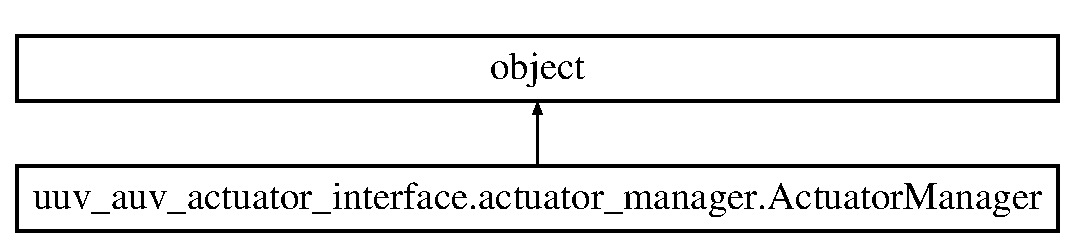
\includegraphics[height=2.000000cm]{classuuv__auv__actuator__interface_1_1actuator__manager_1_1ActuatorManager}
\end{center}
\end{figure}
\subsection*{Public Member Functions}
\begin{DoxyCompactItemize}
\item 
\mbox{\Hypertarget{classuuv__auv__actuator__interface_1_1actuator__manager_1_1ActuatorManager_ad6d3d9b99024a1a0f5fdbc6be598f77d}\label{classuuv__auv__actuator__interface_1_1actuator__manager_1_1ActuatorManager_ad6d3d9b99024a1a0f5fdbc6be598f77d}} 
def {\bfseries \+\_\+\+\_\+init\+\_\+\+\_\+} (self)
\item 
def \hyperlink{classuuv__auv__actuator__interface_1_1actuator__manager_1_1ActuatorManager_a1c8c06aa3e9a62acff2b4002f7b02dd2}{find\+\_\+actuators} (self)
\item 
\mbox{\Hypertarget{classuuv__auv__actuator__interface_1_1actuator__manager_1_1ActuatorManager_a1c55d2294a80e5e86e77271dfd7f957d}\label{classuuv__auv__actuator__interface_1_1actuator__manager_1_1ActuatorManager_a1c55d2294a80e5e86e77271dfd7f957d}} 
def {\bfseries compute\+\_\+control\+\_\+force} (self, thrust, delta, u)
\item 
\mbox{\Hypertarget{classuuv__auv__actuator__interface_1_1actuator__manager_1_1ActuatorManager_abb2b0265a2173b5ecde7b51124fcf943}\label{classuuv__auv__actuator__interface_1_1actuator__manager_1_1ActuatorManager_abb2b0265a2173b5ecde7b51124fcf943}} 
def {\bfseries publish\+\_\+commands} (self, command)
\end{DoxyCompactItemize}
\subsection*{Public Attributes}
\begin{DoxyCompactItemize}
\item 
\mbox{\Hypertarget{classuuv__auv__actuator__interface_1_1actuator__manager_1_1ActuatorManager_a101d9341c0e857b417040817a55272dc}\label{classuuv__auv__actuator__interface_1_1actuator__manager_1_1ActuatorManager_a101d9341c0e857b417040817a55272dc}} 
{\bfseries namespace}
\item 
\mbox{\Hypertarget{classuuv__auv__actuator__interface_1_1actuator__manager_1_1ActuatorManager_af546a41e7a29642da6456ae31ea25024}\label{classuuv__auv__actuator__interface_1_1actuator__manager_1_1ActuatorManager_af546a41e7a29642da6456ae31ea25024}} 
{\bfseries tf\+\_\+buffer}
\item 
\mbox{\Hypertarget{classuuv__auv__actuator__interface_1_1actuator__manager_1_1ActuatorManager_a595861bc3ef889e0b71c67de3317df3c}\label{classuuv__auv__actuator__interface_1_1actuator__manager_1_1ActuatorManager_a595861bc3ef889e0b71c67de3317df3c}} 
{\bfseries listener}
\item 
\mbox{\Hypertarget{classuuv__auv__actuator__interface_1_1actuator__manager_1_1ActuatorManager_af3f8b4c298080d9f602ecff704031172}\label{classuuv__auv__actuator__interface_1_1actuator__manager_1_1ActuatorManager_af3f8b4c298080d9f602ecff704031172}} 
{\bfseries base\+\_\+link\+\_\+ned\+\_\+to\+\_\+enu}
\item 
\mbox{\Hypertarget{classuuv__auv__actuator__interface_1_1actuator__manager_1_1ActuatorManager_ad455d13e9a08f3d6d603ecf5b6c99a81}\label{classuuv__auv__actuator__interface_1_1actuator__manager_1_1ActuatorManager_ad455d13e9a08f3d6d603ecf5b6c99a81}} 
{\bfseries base\+\_\+link}
\item 
\mbox{\Hypertarget{classuuv__auv__actuator__interface_1_1actuator__manager_1_1ActuatorManager_a5bbdfb6c026071a3a31af937bf5223c4}\label{classuuv__auv__actuator__interface_1_1actuator__manager_1_1ActuatorManager_a5bbdfb6c026071a3a31af937bf5223c4}} 
{\bfseries thruster\+\_\+config}
\item 
\mbox{\Hypertarget{classuuv__auv__actuator__interface_1_1actuator__manager_1_1ActuatorManager_a4ffa669e1a096e7062edd76486b69f6b}\label{classuuv__auv__actuator__interface_1_1actuator__manager_1_1ActuatorManager_a4ffa669e1a096e7062edd76486b69f6b}} 
{\bfseries thruster\+\_\+topic}
\item 
\mbox{\Hypertarget{classuuv__auv__actuator__interface_1_1actuator__manager_1_1ActuatorManager_afd2f437f3f3b1cc293fbe479d6b9f378}\label{classuuv__auv__actuator__interface_1_1actuator__manager_1_1ActuatorManager_afd2f437f3f3b1cc293fbe479d6b9f378}} 
{\bfseries thruster}
\item 
\mbox{\Hypertarget{classuuv__auv__actuator__interface_1_1actuator__manager_1_1ActuatorManager_a073b0ba2da3b68c230a45bb892dfa0db}\label{classuuv__auv__actuator__interface_1_1actuator__manager_1_1ActuatorManager_a073b0ba2da3b68c230a45bb892dfa0db}} 
{\bfseries fin\+\_\+config}
\item 
\mbox{\Hypertarget{classuuv__auv__actuator__interface_1_1actuator__manager_1_1ActuatorManager_a61156b94f291441d1a204b1d2ab2284e}\label{classuuv__auv__actuator__interface_1_1actuator__manager_1_1ActuatorManager_a61156b94f291441d1a204b1d2ab2284e}} 
{\bfseries fin\+\_\+lower\+\_\+limit}
\item 
\mbox{\Hypertarget{classuuv__auv__actuator__interface_1_1actuator__manager_1_1ActuatorManager_a1d64a9b3e9df832695fe680b5fef2f1b}\label{classuuv__auv__actuator__interface_1_1actuator__manager_1_1ActuatorManager_a1d64a9b3e9df832695fe680b5fef2f1b}} 
{\bfseries fin\+\_\+upper\+\_\+limit}
\item 
\mbox{\Hypertarget{classuuv__auv__actuator__interface_1_1actuator__manager_1_1ActuatorManager_a0c689385a61f867a96fa510a6949bb37}\label{classuuv__auv__actuator__interface_1_1actuator__manager_1_1ActuatorManager_a0c689385a61f867a96fa510a6949bb37}} 
{\bfseries fins}
\item 
\mbox{\Hypertarget{classuuv__auv__actuator__interface_1_1actuator__manager_1_1ActuatorManager_a4b67111d4acbbba204f24dea8d2e422d}\label{classuuv__auv__actuator__interface_1_1actuator__manager_1_1ActuatorManager_a4b67111d4acbbba204f24dea8d2e422d}} 
{\bfseries n\+\_\+fins}
\item 
\mbox{\Hypertarget{classuuv__auv__actuator__interface_1_1actuator__manager_1_1ActuatorManager_a2e6c90a55300d686b86a3dc8fa03aebd}\label{classuuv__auv__actuator__interface_1_1actuator__manager_1_1ActuatorManager_a2e6c90a55300d686b86a3dc8fa03aebd}} 
{\bfseries ready}
\end{DoxyCompactItemize}
\subsection*{Static Public Attributes}
\begin{DoxyCompactItemize}
\item 
\mbox{\Hypertarget{classuuv__auv__actuator__interface_1_1actuator__manager_1_1ActuatorManager_a9722051810c0aa56d83098b90c8ac732}\label{classuuv__auv__actuator__interface_1_1actuator__manager_1_1ActuatorManager_a9722051810c0aa56d83098b90c8ac732}} 
int {\bfseries M\+A\+X\+\_\+\+F\+I\+NS} = 4
\end{DoxyCompactItemize}


\subsection{Member Function Documentation}
\mbox{\Hypertarget{classuuv__auv__actuator__interface_1_1actuator__manager_1_1ActuatorManager_a1c8c06aa3e9a62acff2b4002f7b02dd2}\label{classuuv__auv__actuator__interface_1_1actuator__manager_1_1ActuatorManager_a1c8c06aa3e9a62acff2b4002f7b02dd2}} 
\index{uuv\+\_\+auv\+\_\+actuator\+\_\+interface\+::actuator\+\_\+manager\+::\+Actuator\+Manager@{uuv\+\_\+auv\+\_\+actuator\+\_\+interface\+::actuator\+\_\+manager\+::\+Actuator\+Manager}!find\+\_\+actuators@{find\+\_\+actuators}}
\index{find\+\_\+actuators@{find\+\_\+actuators}!uuv\+\_\+auv\+\_\+actuator\+\_\+interface\+::actuator\+\_\+manager\+::\+Actuator\+Manager@{uuv\+\_\+auv\+\_\+actuator\+\_\+interface\+::actuator\+\_\+manager\+::\+Actuator\+Manager}}
\subsubsection{\texorpdfstring{find\+\_\+actuators()}{find\_actuators()}}
{\footnotesize\ttfamily def uuv\+\_\+auv\+\_\+actuator\+\_\+interface.\+actuator\+\_\+manager.\+Actuator\+Manager.\+find\+\_\+actuators (\begin{DoxyParamCaption}\item[{}]{self }\end{DoxyParamCaption})}

\begin{DoxyVerb}Calculate the control allocation matrix, if one is not given.\end{DoxyVerb}
 

The documentation for this class was generated from the following file\+:\begin{DoxyCompactItemize}
\item 
control\+\_\+layer/uuv\+\_\+auv\+\_\+control\+\_\+allocator/src/uuv\+\_\+auv\+\_\+actuator\+\_\+interface/actuator\+\_\+manager.\+py\end{DoxyCompactItemize}

\hypertarget{classmaster__layer_1_1anahita__thruster__manager_1_1AnahitaThrusterManager}{}\section{master\+\_\+layer.\+anahita\+\_\+thruster\+\_\+manager.\+Anahita\+Thruster\+Manager Class Reference}
\label{classmaster__layer_1_1anahita__thruster__manager_1_1AnahitaThrusterManager}\index{master\+\_\+layer.\+anahita\+\_\+thruster\+\_\+manager.\+Anahita\+Thruster\+Manager@{master\+\_\+layer.\+anahita\+\_\+thruster\+\_\+manager.\+Anahita\+Thruster\+Manager}}
Inheritance diagram for master\+\_\+layer.\+anahita\+\_\+thruster\+\_\+manager.\+Anahita\+Thruster\+Manager\+:\begin{figure}[H]
\begin{center}
\leavevmode
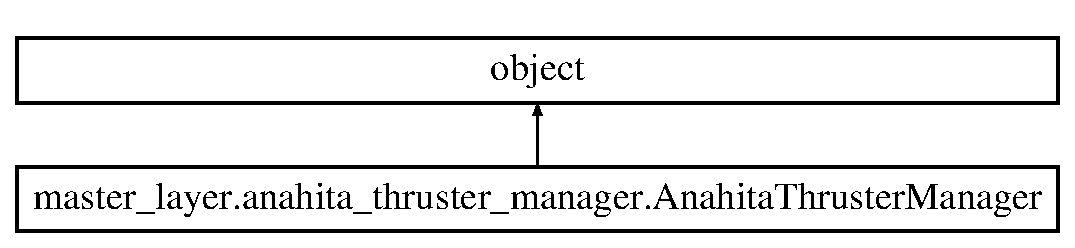
\includegraphics[height=2.000000cm]{classmaster__layer_1_1anahita__thruster__manager_1_1AnahitaThrusterManager}
\end{center}
\end{figure}
\subsection*{Public Member Functions}
\begin{DoxyCompactItemize}
\item 
\mbox{\Hypertarget{classmaster__layer_1_1anahita__thruster__manager_1_1AnahitaThrusterManager_a51137f1973d4db38374e401a500bc8e8}\label{classmaster__layer_1_1anahita__thruster__manager_1_1AnahitaThrusterManager_a51137f1973d4db38374e401a500bc8e8}} 
def {\bfseries \+\_\+\+\_\+init\+\_\+\+\_\+} (self, arg, kwargs)
\item 
\mbox{\Hypertarget{classmaster__layer_1_1anahita__thruster__manager_1_1AnahitaThrusterManager_a00ee062fb635fe83f7aa5177869bd8ce}\label{classmaster__layer_1_1anahita__thruster__manager_1_1AnahitaThrusterManager_a00ee062fb635fe83f7aa5177869bd8ce}} 
def {\bfseries compute\+\_\+pwm} (self, thrust)
\item 
\mbox{\Hypertarget{classmaster__layer_1_1anahita__thruster__manager_1_1AnahitaThrusterManager_a7a10f8f3dd09bb0cce566758a856f2d5}\label{classmaster__layer_1_1anahita__thruster__manager_1_1AnahitaThrusterManager_a7a10f8f3dd09bb0cce566758a856f2d5}} 
def {\bfseries input\+\_\+callback} (self, msg)
\item 
def \hyperlink{classmaster__layer_1_1anahita__thruster__manager_1_1AnahitaThrusterManager_ad4dd17de08cd3f4f455d98aa584caf24}{compute\+\_\+thruster\+\_\+forces} (self, gen\+\_\+forces)
\item 
def \hyperlink{classmaster__layer_1_1anahita__thruster__manager_1_1AnahitaThrusterManager_adbd3b3d5485e9c627943896f2b2403c1}{command\+\_\+thrusters} (self)
\end{DoxyCompactItemize}
\subsection*{Public Attributes}
\begin{DoxyCompactItemize}
\item 
\mbox{\Hypertarget{classmaster__layer_1_1anahita__thruster__manager_1_1AnahitaThrusterManager_ac95d72fff1b8added7c3773b9ee77b24}\label{classmaster__layer_1_1anahita__thruster__manager_1_1AnahitaThrusterManager_ac95d72fff1b8added7c3773b9ee77b24}} 
{\bfseries n\+\_\+thrusters}
\item 
\mbox{\Hypertarget{classmaster__layer_1_1anahita__thruster__manager_1_1AnahitaThrusterManager_a26d42e3aded66ec75062e6abbe679a3c}\label{classmaster__layer_1_1anahita__thruster__manager_1_1AnahitaThrusterManager_a26d42e3aded66ec75062e6abbe679a3c}} 
{\bfseries configuration\+\_\+matrix}
\item 
\mbox{\Hypertarget{classmaster__layer_1_1anahita__thruster__manager_1_1AnahitaThrusterManager_a4b731e2105fe0c18791c6d8575bc13ef}\label{classmaster__layer_1_1anahita__thruster__manager_1_1AnahitaThrusterManager_a4b731e2105fe0c18791c6d8575bc13ef}} 
{\bfseries inverse\+\_\+configuration\+\_\+matrix}
\item 
\mbox{\Hypertarget{classmaster__layer_1_1anahita__thruster__manager_1_1AnahitaThrusterManager_ac79d96f2b6ce722625d6e0093867c240}\label{classmaster__layer_1_1anahita__thruster__manager_1_1AnahitaThrusterManager_ac79d96f2b6ce722625d6e0093867c240}} 
{\bfseries input\+\_\+sub}
\item 
\mbox{\Hypertarget{classmaster__layer_1_1anahita__thruster__manager_1_1AnahitaThrusterManager_ac93d7950c085702c8f3bd1d271058c04}\label{classmaster__layer_1_1anahita__thruster__manager_1_1AnahitaThrusterManager_ac93d7950c085702c8f3bd1d271058c04}} 
{\bfseries pwm\+\_\+pub}
\item 
\mbox{\Hypertarget{classmaster__layer_1_1anahita__thruster__manager_1_1AnahitaThrusterManager_ae8bc0f83f0e585df90793b7f2b84e46b}\label{classmaster__layer_1_1anahita__thruster__manager_1_1AnahitaThrusterManager_ae8bc0f83f0e585df90793b7f2b84e46b}} 
{\bfseries thrust}
\item 
\mbox{\Hypertarget{classmaster__layer_1_1anahita__thruster__manager_1_1AnahitaThrusterManager_ab4497b87e68af18ea8c658a4ad01f8fb}\label{classmaster__layer_1_1anahita__thruster__manager_1_1AnahitaThrusterManager_ab4497b87e68af18ea8c658a4ad01f8fb}} 
{\bfseries ready}
\end{DoxyCompactItemize}


\subsection{Member Function Documentation}
\mbox{\Hypertarget{classmaster__layer_1_1anahita__thruster__manager_1_1AnahitaThrusterManager_adbd3b3d5485e9c627943896f2b2403c1}\label{classmaster__layer_1_1anahita__thruster__manager_1_1AnahitaThrusterManager_adbd3b3d5485e9c627943896f2b2403c1}} 
\index{master\+\_\+layer\+::anahita\+\_\+thruster\+\_\+manager\+::\+Anahita\+Thruster\+Manager@{master\+\_\+layer\+::anahita\+\_\+thruster\+\_\+manager\+::\+Anahita\+Thruster\+Manager}!command\+\_\+thrusters@{command\+\_\+thrusters}}
\index{command\+\_\+thrusters@{command\+\_\+thrusters}!master\+\_\+layer\+::anahita\+\_\+thruster\+\_\+manager\+::\+Anahita\+Thruster\+Manager@{master\+\_\+layer\+::anahita\+\_\+thruster\+\_\+manager\+::\+Anahita\+Thruster\+Manager}}
\subsubsection{\texorpdfstring{command\+\_\+thrusters()}{command\_thrusters()}}
{\footnotesize\ttfamily def master\+\_\+layer.\+anahita\+\_\+thruster\+\_\+manager.\+Anahita\+Thruster\+Manager.\+command\+\_\+thrusters (\begin{DoxyParamCaption}\item[{}]{self }\end{DoxyParamCaption})}

\begin{DoxyVerb}Publish the thruster input into their specific topic.\end{DoxyVerb}
 \mbox{\Hypertarget{classmaster__layer_1_1anahita__thruster__manager_1_1AnahitaThrusterManager_ad4dd17de08cd3f4f455d98aa584caf24}\label{classmaster__layer_1_1anahita__thruster__manager_1_1AnahitaThrusterManager_ad4dd17de08cd3f4f455d98aa584caf24}} 
\index{master\+\_\+layer\+::anahita\+\_\+thruster\+\_\+manager\+::\+Anahita\+Thruster\+Manager@{master\+\_\+layer\+::anahita\+\_\+thruster\+\_\+manager\+::\+Anahita\+Thruster\+Manager}!compute\+\_\+thruster\+\_\+forces@{compute\+\_\+thruster\+\_\+forces}}
\index{compute\+\_\+thruster\+\_\+forces@{compute\+\_\+thruster\+\_\+forces}!master\+\_\+layer\+::anahita\+\_\+thruster\+\_\+manager\+::\+Anahita\+Thruster\+Manager@{master\+\_\+layer\+::anahita\+\_\+thruster\+\_\+manager\+::\+Anahita\+Thruster\+Manager}}
\subsubsection{\texorpdfstring{compute\+\_\+thruster\+\_\+forces()}{compute\_thruster\_forces()}}
{\footnotesize\ttfamily def master\+\_\+layer.\+anahita\+\_\+thruster\+\_\+manager.\+Anahita\+Thruster\+Manager.\+compute\+\_\+thruster\+\_\+forces (\begin{DoxyParamCaption}\item[{}]{self,  }\item[{}]{gen\+\_\+forces }\end{DoxyParamCaption})}

\begin{DoxyVerb}Compute desired thruster forces using the inverse configuration
matrix.
\end{DoxyVerb}
 

The documentation for this class was generated from the following file\+:\begin{DoxyCompactItemize}
\item 
master\+\_\+layer/src/master\+\_\+layer/anahita\+\_\+thruster\+\_\+manager.\+py\end{DoxyCompactItemize}

\hypertarget{classBase__class}{}\section{Base\+\_\+class Class Reference}
\label{classBase__class}\index{Base\+\_\+class@{Base\+\_\+class}}
Inheritance diagram for Base\+\_\+class\+:\begin{figure}[H]
\begin{center}
\leavevmode
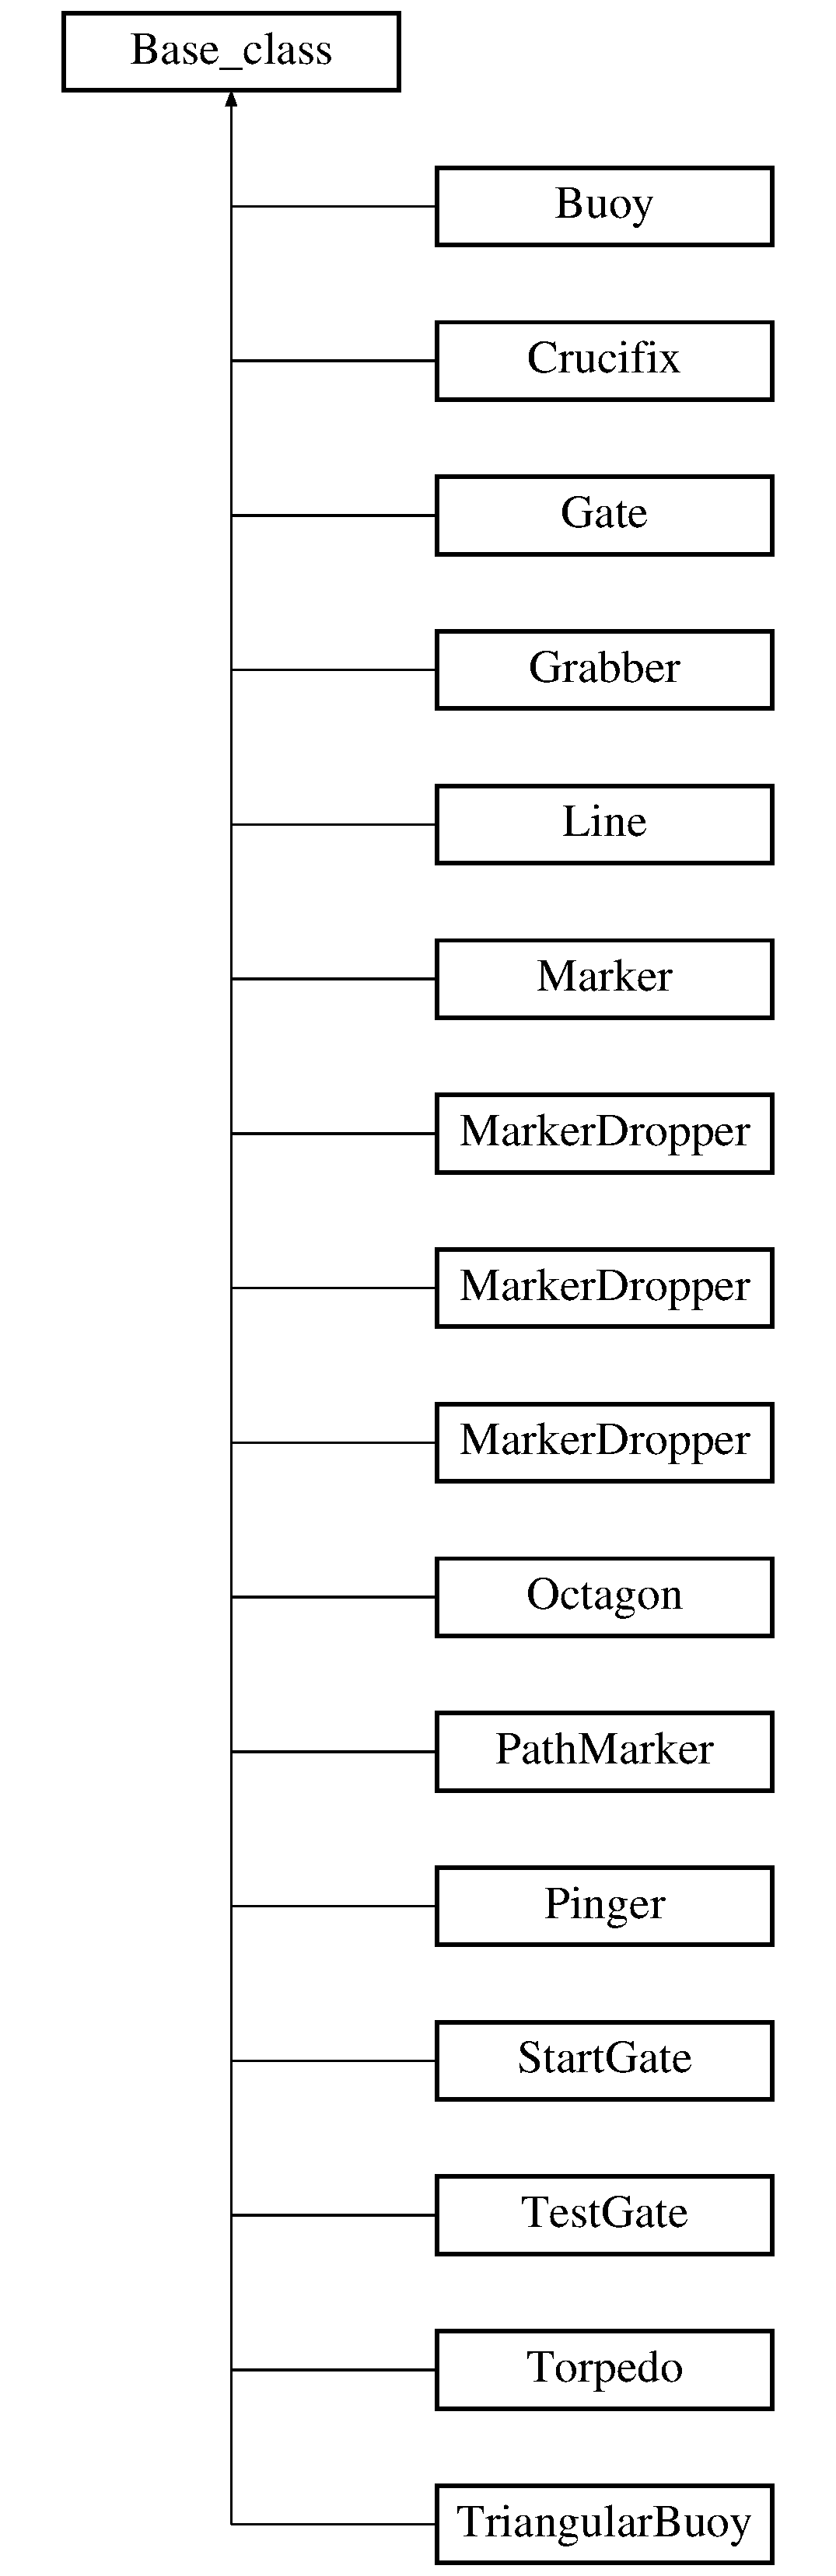
\includegraphics[height=12.000000cm]{classBase__class}
\end{center}
\end{figure}
\subsection*{Public Member Functions}
\begin{DoxyCompactItemize}
\item 
\mbox{\Hypertarget{classBase__class_af6a0b08cc6b142bd06568953346a7510}\label{classBase__class_af6a0b08cc6b142bd06568953346a7510}} 
virtual void {\bfseries spin\+Thread\+Front} ()
\item 
\mbox{\Hypertarget{classBase__class_a697ded45cee7fb2426458bb5b0105f00}\label{classBase__class_a697ded45cee7fb2426458bb5b0105f00}} 
virtual void {\bfseries spin\+Thread\+Bottom} ()
\item 
\mbox{\Hypertarget{classBase__class_a5bda5f5f5716cc83558677c60a2c4bc6}\label{classBase__class_a5bda5f5f5716cc83558677c60a2c4bc6}} 
void {\bfseries bottom\+Task\+Handling} (bool status)
\item 
\mbox{\Hypertarget{classBase__class_abdfc7986221e6db12d267aa74736ca40}\label{classBase__class_abdfc7986221e6db12d267aa74736ca40}} 
void {\bfseries front\+Task\+Handling} (bool status)
\item 
\mbox{\Hypertarget{classBase__class_a609e2b04688ea241e3dc2a6c1be25b21}\label{classBase__class_a609e2b04688ea241e3dc2a6c1be25b21}} 
void {\bfseries image\+Front\+Callback} (const sensor\+\_\+msgs\+::\+Image\+::\+Const\+Ptr \&msg)
\item 
\mbox{\Hypertarget{classBase__class_a3d9f198134835742ca0bc332ca52be3a}\label{classBase__class_a3d9f198134835742ca0bc332ca52be3a}} 
void {\bfseries image\+Bottom\+Callback} (const sensor\+\_\+msgs\+::\+Image\+::\+Const\+Ptr \&msg)
\item 
\mbox{\Hypertarget{classBase__class_ada15311e090a1017747a2040b47b8430}\label{classBase__class_ada15311e090a1017747a2040b47b8430}} 
void {\bfseries fusion\+Callback} (const sensor\+\_\+msgs\+::\+Image\+::\+Const\+Ptr \&msg)
\item 
\mbox{\Hypertarget{classBase__class_a5c1d64c9bbbaa631396a2aea655df5a0}\label{classBase__class_a5c1d64c9bbbaa631396a2aea655df5a0}} 
virtual void {\bfseries load\+Params} ()
\item 
\mbox{\Hypertarget{classBase__class_a5b23d53f25b7fc2fb20536b94a1e054e}\label{classBase__class_a5b23d53f25b7fc2fb20536b94a1e054e}} 
void {\bfseries init} ()
\end{DoxyCompactItemize}
\subsection*{Public Attributes}
\begin{DoxyCompactItemize}
\item 
\mbox{\Hypertarget{classBase__class_a0c637b9d05ba44ce2d9b72325f55b93e}\label{classBase__class_a0c637b9d05ba44ce2d9b72325f55b93e}} 
ros\+::\+Node\+Handle {\bfseries nh}
\item 
\mbox{\Hypertarget{classBase__class_a220ef4029efe5d7f0e6a2f05ed243ca7}\label{classBase__class_a220ef4029efe5d7f0e6a2f05ed243ca7}} 
image\+\_\+transport\+::\+Image\+Transport {\bfseries it}
\item 
\mbox{\Hypertarget{classBase__class_a4dc6972ad9bc616b6430a631bd03defa}\label{classBase__class_a4dc6972ad9bc616b6430a631bd03defa}} 
std\+\_\+msgs\+::\+Float32 {\bfseries front\+\_\+x\+\_\+coordinate}
\item 
\mbox{\Hypertarget{classBase__class_a093214b7b4e70f5c5aa08acc9c650882}\label{classBase__class_a093214b7b4e70f5c5aa08acc9c650882}} 
std\+\_\+msgs\+::\+Float32 {\bfseries front\+\_\+y\+\_\+coordinate}
\item 
\mbox{\Hypertarget{classBase__class_a1dc276a367c03d2a54516613bc8005f4}\label{classBase__class_a1dc276a367c03d2a54516613bc8005f4}} 
std\+\_\+msgs\+::\+Float32 {\bfseries front\+\_\+z\+\_\+coordinate}
\item 
\mbox{\Hypertarget{classBase__class_a30acee1702ef9b5cb42032ba5c451276}\label{classBase__class_a30acee1702ef9b5cb42032ba5c451276}} 
std\+\_\+msgs\+::\+Float32 {\bfseries bottom\+\_\+x\+\_\+coordinate}
\item 
\mbox{\Hypertarget{classBase__class_a8ff5e8a73f05506118a9d442c1a8a99b}\label{classBase__class_a8ff5e8a73f05506118a9d442c1a8a99b}} 
std\+\_\+msgs\+::\+Float32 {\bfseries bottom\+\_\+y\+\_\+coordinate}
\item 
\mbox{\Hypertarget{classBase__class_ad1a1fcdaaa8103c14d66ad2d1efa00f2}\label{classBase__class_ad1a1fcdaaa8103c14d66ad2d1efa00f2}} 
std\+\_\+msgs\+::\+Float32 {\bfseries bottom\+\_\+z\+\_\+coordinate}
\item 
\mbox{\Hypertarget{classBase__class_a17f406063739c71815f4bbe990ef4df0}\label{classBase__class_a17f406063739c71815f4bbe990ef4df0}} 
cv\+::\+Mat {\bfseries image\+\_\+front}
\item 
\mbox{\Hypertarget{classBase__class_a093e57e2b6f567e565738c89964d3e24}\label{classBase__class_a093e57e2b6f567e565738c89964d3e24}} 
cv\+::\+Mat {\bfseries image\+\_\+bottom}
\item 
\mbox{\Hypertarget{classBase__class_a264c83f603564a202a99c92f2510f482}\label{classBase__class_a264c83f603564a202a99c92f2510f482}} 
cv\+::\+Mat {\bfseries image\+\_\+front\+\_\+marked}
\item 
\mbox{\Hypertarget{classBase__class_adfc9d9fff23510b891419d7c5f2d7827}\label{classBase__class_adfc9d9fff23510b891419d7c5f2d7827}} 
cv\+::\+Mat {\bfseries image\+\_\+bottom\+\_\+marked}
\item 
\mbox{\Hypertarget{classBase__class_a0e1bde28a76383990023456ae5ec7547}\label{classBase__class_a0e1bde28a76383990023456ae5ec7547}} 
cv\+::\+Mat {\bfseries image\+\_\+front\+\_\+thresholded}
\item 
\mbox{\Hypertarget{classBase__class_a317c340910484b105b50afeffa0d651c}\label{classBase__class_a317c340910484b105b50afeffa0d651c}} 
cv\+::\+Mat {\bfseries image\+\_\+bottom\+\_\+thresholded}
\item 
\mbox{\Hypertarget{classBase__class_a6ce39edcefc3ffa24874c7792b3b8893}\label{classBase__class_a6ce39edcefc3ffa24874c7792b3b8893}} 
cv\+::\+Mat {\bfseries enhanced\+\_\+image}
\item 
\mbox{\Hypertarget{classBase__class_a43259df646d0d87bfedc522d11f2fe3e}\label{classBase__class_a43259df646d0d87bfedc522d11f2fe3e}} 
boost\+::thread $\ast$ {\bfseries spin\+\_\+thread\+\_\+bottom}
\item 
\mbox{\Hypertarget{classBase__class_a2385294c29c4ddd09a9a212c1594af40}\label{classBase__class_a2385294c29c4ddd09a9a212c1594af40}} 
boost\+::thread $\ast$ {\bfseries spin\+\_\+thread\+\_\+front}
\item 
\mbox{\Hypertarget{classBase__class_a5b5116111776bd3e2d47bbcb80e2b0a0}\label{classBase__class_a5b5116111776bd3e2d47bbcb80e2b0a0}} 
std\+::mutex {\bfseries vision\+\_\+mutex}
\end{DoxyCompactItemize}
\subsection*{Protected Attributes}
\begin{DoxyCompactItemize}
\item 
\mbox{\Hypertarget{classBase__class_a8f80b6bad9eee41faadc3fe618c9fbce}\label{classBase__class_a8f80b6bad9eee41faadc3fe618c9fbce}} 
int {\bfseries front\+\_\+low\+\_\+g\+\_\+}
\item 
\mbox{\Hypertarget{classBase__class_aa325e45d069b2871559985dc59feeccc}\label{classBase__class_aa325e45d069b2871559985dc59feeccc}} 
int {\bfseries front\+\_\+high\+\_\+g\+\_\+}
\item 
\mbox{\Hypertarget{classBase__class_ac9a0ac60d6392d2747bdbc11cbbedec4}\label{classBase__class_ac9a0ac60d6392d2747bdbc11cbbedec4}} 
int {\bfseries front\+\_\+low\+\_\+r\+\_\+}
\item 
\mbox{\Hypertarget{classBase__class_adddda44e0a8e5983ca3918d4aa26636a}\label{classBase__class_adddda44e0a8e5983ca3918d4aa26636a}} 
int {\bfseries front\+\_\+high\+\_\+r\+\_\+}
\item 
\mbox{\Hypertarget{classBase__class_a44d4c2ad6afa54c8d2dd382a9a67227c}\label{classBase__class_a44d4c2ad6afa54c8d2dd382a9a67227c}} 
int {\bfseries front\+\_\+low\+\_\+b\+\_\+}
\item 
\mbox{\Hypertarget{classBase__class_a166bca19ec2cbba93190b7f5063ee43d}\label{classBase__class_a166bca19ec2cbba93190b7f5063ee43d}} 
int {\bfseries front\+\_\+high\+\_\+b\+\_\+}
\item 
\mbox{\Hypertarget{classBase__class_aafa05dd2f63849129a9edc77eb827798}\label{classBase__class_aafa05dd2f63849129a9edc77eb827798}} 
int {\bfseries front\+\_\+opening\+\_\+mat\+\_\+point\+\_\+}
\item 
\mbox{\Hypertarget{classBase__class_a673c6e2b5d99afa183bab9a86e8e03d3}\label{classBase__class_a673c6e2b5d99afa183bab9a86e8e03d3}} 
int {\bfseries front\+\_\+opening\+\_\+iter\+\_\+}
\item 
\mbox{\Hypertarget{classBase__class_abf41eb7847f92747d8756e75a5fd16d2}\label{classBase__class_abf41eb7847f92747d8756e75a5fd16d2}} 
int {\bfseries front\+\_\+closing\+\_\+mat\+\_\+point\+\_\+}
\item 
\mbox{\Hypertarget{classBase__class_a4a1fe1615bacad22704a3c7c6df24c6b}\label{classBase__class_a4a1fe1615bacad22704a3c7c6df24c6b}} 
int {\bfseries front\+\_\+closing\+\_\+iter\+\_\+}
\item 
\mbox{\Hypertarget{classBase__class_a60ba75930ed3441e171fd33f468ab8f3}\label{classBase__class_a60ba75930ed3441e171fd33f468ab8f3}} 
int {\bfseries front\+\_\+bilateral\+\_\+iter\+\_\+}
\item 
\mbox{\Hypertarget{classBase__class_ac34dae2ec32d35a295daa2a154d8ebc2}\label{classBase__class_ac34dae2ec32d35a295daa2a154d8ebc2}} 
int {\bfseries bottom\+\_\+low\+\_\+g\+\_\+}
\item 
\mbox{\Hypertarget{classBase__class_a5577fab7b6d2905b1077d231a9427c78}\label{classBase__class_a5577fab7b6d2905b1077d231a9427c78}} 
int {\bfseries bottom\+\_\+low\+\_\+r\+\_\+}
\item 
\mbox{\Hypertarget{classBase__class_a9f15b22c0795cd5c3321cbb6a319c852}\label{classBase__class_a9f15b22c0795cd5c3321cbb6a319c852}} 
int {\bfseries bottom\+\_\+low\+\_\+b\+\_\+}
\item 
\mbox{\Hypertarget{classBase__class_a87ec3d96e723540665817ed9393d39f2}\label{classBase__class_a87ec3d96e723540665817ed9393d39f2}} 
int {\bfseries bottom\+\_\+high\+\_\+g\+\_\+}
\item 
\mbox{\Hypertarget{classBase__class_a0dd97c1db7d7466db46a066a5a94c6f5}\label{classBase__class_a0dd97c1db7d7466db46a066a5a94c6f5}} 
int {\bfseries bottom\+\_\+high\+\_\+r\+\_\+}
\item 
\mbox{\Hypertarget{classBase__class_a15b47c73142453acc22e8ef5fb7a4c31}\label{classBase__class_a15b47c73142453acc22e8ef5fb7a4c31}} 
int {\bfseries bottom\+\_\+high\+\_\+b\+\_\+}
\item 
\mbox{\Hypertarget{classBase__class_ab8bf6aeb0e7e35cc2cbb78c748161dcd}\label{classBase__class_ab8bf6aeb0e7e35cc2cbb78c748161dcd}} 
int {\bfseries bottom\+\_\+closing\+\_\+mat\+\_\+point\+\_\+}
\item 
\mbox{\Hypertarget{classBase__class_af1aed74bec81e65fbc49f508478d9402}\label{classBase__class_af1aed74bec81e65fbc49f508478d9402}} 
int {\bfseries bottom\+\_\+closing\+\_\+iter\+\_\+}
\item 
\mbox{\Hypertarget{classBase__class_a26ad84dbcddebb9bfa86c60e20d420c4}\label{classBase__class_a26ad84dbcddebb9bfa86c60e20d420c4}} 
int {\bfseries bottom\+\_\+opening\+\_\+iter\+\_\+}
\item 
\mbox{\Hypertarget{classBase__class_ade092108e623d30416d602cd5cae744f}\label{classBase__class_ade092108e623d30416d602cd5cae744f}} 
int {\bfseries bottom\+\_\+opening\+\_\+mat\+\_\+point\+\_\+}
\item 
\mbox{\Hypertarget{classBase__class_a39d5fecdbca5b67275c5190e545b84d6}\label{classBase__class_a39d5fecdbca5b67275c5190e545b84d6}} 
int {\bfseries bottom\+\_\+bilateral\+\_\+iter\+\_\+}
\item 
\mbox{\Hypertarget{classBase__class_ae03833accc82e68126825245dc1982fa}\label{classBase__class_ae03833accc82e68126825245dc1982fa}} 
bool {\bfseries close\+\_\+task} = false
\item 
\mbox{\Hypertarget{classBase__class_a4e631c16dc345e509bdeeeefe7fea10c}\label{classBase__class_a4e631c16dc345e509bdeeeefe7fea10c}} 
image\+\_\+transport\+::\+Subscriber {\bfseries front\+\_\+image\+\_\+sub}
\item 
\mbox{\Hypertarget{classBase__class_a271cb980412b067997fc97d9693952c2}\label{classBase__class_a271cb980412b067997fc97d9693952c2}} 
image\+\_\+transport\+::\+Subscriber {\bfseries bottom\+\_\+image\+\_\+sub}
\item 
\mbox{\Hypertarget{classBase__class_a2597f44ae992acb9346c5236981dde8a}\label{classBase__class_a2597f44ae992acb9346c5236981dde8a}} 
image\+\_\+transport\+::\+Subscriber {\bfseries enhanced\+\_\+image\+\_\+sub}
\item 
\mbox{\Hypertarget{classBase__class_a39c380a01e7bd17d10feadb1422b3d32}\label{classBase__class_a39c380a01e7bd17d10feadb1422b3d32}} 
image\+\_\+transport\+::\+Publisher {\bfseries bottom\+\_\+thresholded\+\_\+pub}
\item 
\mbox{\Hypertarget{classBase__class_aa6ba450a5a291ca101a51767a6e8f9b7}\label{classBase__class_aa6ba450a5a291ca101a51767a6e8f9b7}} 
image\+\_\+transport\+::\+Publisher {\bfseries bottom\+\_\+marked\+\_\+pub}
\item 
\mbox{\Hypertarget{classBase__class_abd16a7279fdd1a28794cd6fd5750d9e7}\label{classBase__class_abd16a7279fdd1a28794cd6fd5750d9e7}} 
image\+\_\+transport\+::\+Publisher {\bfseries front\+\_\+thresholded\+\_\+pub}
\item 
\mbox{\Hypertarget{classBase__class_a658ae3fc1783f2cf7b2f58c0e9c83d94}\label{classBase__class_a658ae3fc1783f2cf7b2f58c0e9c83d94}} 
image\+\_\+transport\+::\+Publisher {\bfseries front\+\_\+marked\+\_\+pub}
\item 
\mbox{\Hypertarget{classBase__class_a04bfec1a0dd9622111cc9edcffa5b4ef}\label{classBase__class_a04bfec1a0dd9622111cc9edcffa5b4ef}} 
image\+\_\+transport\+::\+Publisher {\bfseries front\+\_\+edges\+\_\+pub}
\item 
\mbox{\Hypertarget{classBase__class_ab4a69be5b6876ccc175f252a8b914fd8}\label{classBase__class_ab4a69be5b6876ccc175f252a8b914fd8}} 
ros\+::\+Publisher {\bfseries front\+\_\+x\+\_\+coordinate\+\_\+pub}
\item 
\mbox{\Hypertarget{classBase__class_a06b6b24d43c36430aa9acbb5dff10bbc}\label{classBase__class_a06b6b24d43c36430aa9acbb5dff10bbc}} 
ros\+::\+Publisher {\bfseries front\+\_\+y\+\_\+coordinate\+\_\+pub}
\item 
\mbox{\Hypertarget{classBase__class_aedeb44746d27ca5977d17ad1faeb1f9a}\label{classBase__class_aedeb44746d27ca5977d17ad1faeb1f9a}} 
ros\+::\+Publisher {\bfseries front\+\_\+z\+\_\+coordinate\+\_\+pub}
\item 
\mbox{\Hypertarget{classBase__class_a6a7ef2fc8b0c86779d4c2f271b2d4c6f}\label{classBase__class_a6a7ef2fc8b0c86779d4c2f271b2d4c6f}} 
ros\+::\+Publisher {\bfseries bottom\+\_\+x\+\_\+coordinate\+\_\+pub}
\item 
\mbox{\Hypertarget{classBase__class_a125135126a1572aa2511aec025cfc9b6}\label{classBase__class_a125135126a1572aa2511aec025cfc9b6}} 
ros\+::\+Publisher {\bfseries bottom\+\_\+y\+\_\+coordinate\+\_\+pub}
\item 
\mbox{\Hypertarget{classBase__class_a61d6fa33aab9cc448a8cf40c2bddbc6d}\label{classBase__class_a61d6fa33aab9cc448a8cf40c2bddbc6d}} 
ros\+::\+Publisher {\bfseries bottom\+\_\+z\+\_\+coordinate\+\_\+pub}
\item 
\mbox{\Hypertarget{classBase__class_ad248659f61010ebd3c64965a2c70546f}\label{classBase__class_ad248659f61010ebd3c64965a2c70546f}} 
ros\+::\+Publisher {\bfseries detection\+\_\+pub}
\end{DoxyCompactItemize}


The documentation for this class was generated from the following files\+:\begin{DoxyCompactItemize}
\item 
vision\+\_\+layer/vision\+\_\+tasks/include/base\+\_\+class.\+h\item 
vision\+\_\+layer/vision\+\_\+tasks/src/base\+\_\+class.\+cpp\end{DoxyCompactItemize}

\hypertarget{classimage__undistort_1_1BaseCameraParameters}{}\section{image\+\_\+undistort\+:\+:Base\+Camera\+Parameters Class Reference}
\label{classimage__undistort_1_1BaseCameraParameters}\index{image\+\_\+undistort\+::\+Base\+Camera\+Parameters@{image\+\_\+undistort\+::\+Base\+Camera\+Parameters}}
Inheritance diagram for image\+\_\+undistort\+:\+:Base\+Camera\+Parameters\+:\begin{figure}[H]
\begin{center}
\leavevmode
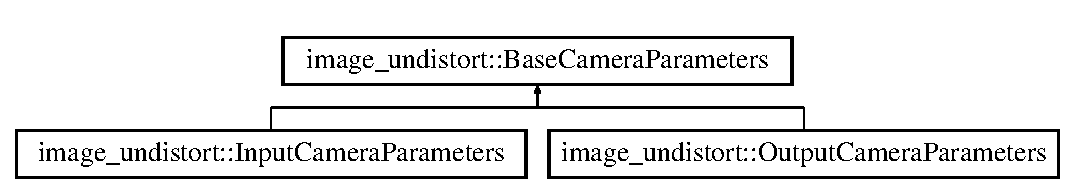
\includegraphics[height=2.000000cm]{classimage__undistort_1_1BaseCameraParameters}
\end{center}
\end{figure}
\subsection*{Public Member Functions}
\begin{DoxyCompactItemize}
\item 
\mbox{\Hypertarget{classimage__undistort_1_1BaseCameraParameters_a88a33425ade97a10aabdae322da2b72b}\label{classimage__undistort_1_1BaseCameraParameters_a88a33425ade97a10aabdae322da2b72b}} 
{\bfseries Base\+Camera\+Parameters} (const ros\+::\+Node\+Handle \&nh, const std\+::string \&camera\+\_\+namespace, const bool invert\+\_\+T)
\item 
\mbox{\Hypertarget{classimage__undistort_1_1BaseCameraParameters_a542e183ba91d54f0ec7f7e5aef5b41c4}\label{classimage__undistort_1_1BaseCameraParameters_a542e183ba91d54f0ec7f7e5aef5b41c4}} 
{\bfseries Base\+Camera\+Parameters} (const sensor\+\_\+msgs\+::\+Camera\+Info \&camera\+\_\+info)
\item 
\mbox{\Hypertarget{classimage__undistort_1_1BaseCameraParameters_a1da0c8f547d638bd1ca788210fd60618}\label{classimage__undistort_1_1BaseCameraParameters_a1da0c8f547d638bd1ca788210fd60618}} 
{\bfseries Base\+Camera\+Parameters} (const cv\+::\+Size \&resolution\+\_\+in, const Eigen\+::\+Matrix$<$ double, 4, 4 $>$ \&T\+\_\+in, const Eigen\+::\+Matrix$<$ double, 3, 3 $>$ \&K\+\_\+in)
\item 
\mbox{\Hypertarget{classimage__undistort_1_1BaseCameraParameters_a9697fe34201dbeedd04cc13050481888}\label{classimage__undistort_1_1BaseCameraParameters_a9697fe34201dbeedd04cc13050481888}} 
const cv\+::\+Size \& {\bfseries resolution} () const
\item 
\mbox{\Hypertarget{classimage__undistort_1_1BaseCameraParameters_a319b23014e690f86f82e8c3c29d9b587}\label{classimage__undistort_1_1BaseCameraParameters_a319b23014e690f86f82e8c3c29d9b587}} 
const Eigen\+::\+Matrix$<$ double, 4, 4 $>$ \& {\bfseries T} () const
\item 
\mbox{\Hypertarget{classimage__undistort_1_1BaseCameraParameters_a3f5a0a253d9db617fa9f83a6be317349}\label{classimage__undistort_1_1BaseCameraParameters_a3f5a0a253d9db617fa9f83a6be317349}} 
const Eigen\+::\+Ref$<$ const Eigen\+::\+Matrix$<$ double, 3, 3 $>$ $>$ {\bfseries R} () const
\item 
\mbox{\Hypertarget{classimage__undistort_1_1BaseCameraParameters_a922498c38ea5853135cfc2445171696d}\label{classimage__undistort_1_1BaseCameraParameters_a922498c38ea5853135cfc2445171696d}} 
const Eigen\+::\+Ref$<$ const Eigen\+::\+Matrix$<$ double, 3, 1 $>$ $>$ {\bfseries p} () const
\item 
\mbox{\Hypertarget{classimage__undistort_1_1BaseCameraParameters_a7c063dab97e59ebaed14f20e6bdf3642}\label{classimage__undistort_1_1BaseCameraParameters_a7c063dab97e59ebaed14f20e6bdf3642}} 
const Eigen\+::\+Matrix$<$ double, 3, 4 $>$ \& {\bfseries P} () const
\item 
\mbox{\Hypertarget{classimage__undistort_1_1BaseCameraParameters_a6de1cedb0186ccd043acd91358763f7e}\label{classimage__undistort_1_1BaseCameraParameters_a6de1cedb0186ccd043acd91358763f7e}} 
const Eigen\+::\+Matrix$<$ double, 3, 3 $>$ \& {\bfseries K} () const
\item 
\mbox{\Hypertarget{classimage__undistort_1_1BaseCameraParameters_a6b2ba6bbe947efe13db70d6ab0700d72}\label{classimage__undistort_1_1BaseCameraParameters_a6b2ba6bbe947efe13db70d6ab0700d72}} 
bool {\bfseries operator==} (const \hyperlink{classimage__undistort_1_1BaseCameraParameters}{Base\+Camera\+Parameters} \&B) const
\item 
\mbox{\Hypertarget{classimage__undistort_1_1BaseCameraParameters_a0e743b0b242034fbfeddecdabb94594f}\label{classimage__undistort_1_1BaseCameraParameters_a0e743b0b242034fbfeddecdabb94594f}} 
bool {\bfseries operator!=} (const \hyperlink{classimage__undistort_1_1BaseCameraParameters}{Base\+Camera\+Parameters} \&B) const
\end{DoxyCompactItemize}


The documentation for this class was generated from the following files\+:\begin{DoxyCompactItemize}
\item 
vision\+\_\+layer/image\+\_\+undistort/include/image\+\_\+undistort/camera\+\_\+parameters.\+h\item 
vision\+\_\+layer/image\+\_\+undistort/src/camera\+\_\+parameters.\+cpp\end{DoxyCompactItemize}

\hypertarget{classmtdef_1_1Baudrates}{}\doxysection{mtdef.\+Baudrates Class Reference}
\label{classmtdef_1_1Baudrates}\index{mtdef.Baudrates@{mtdef.Baudrates}}
Inheritance diagram for mtdef.\+Baudrates\+:\begin{figure}[H]
\begin{center}
\leavevmode
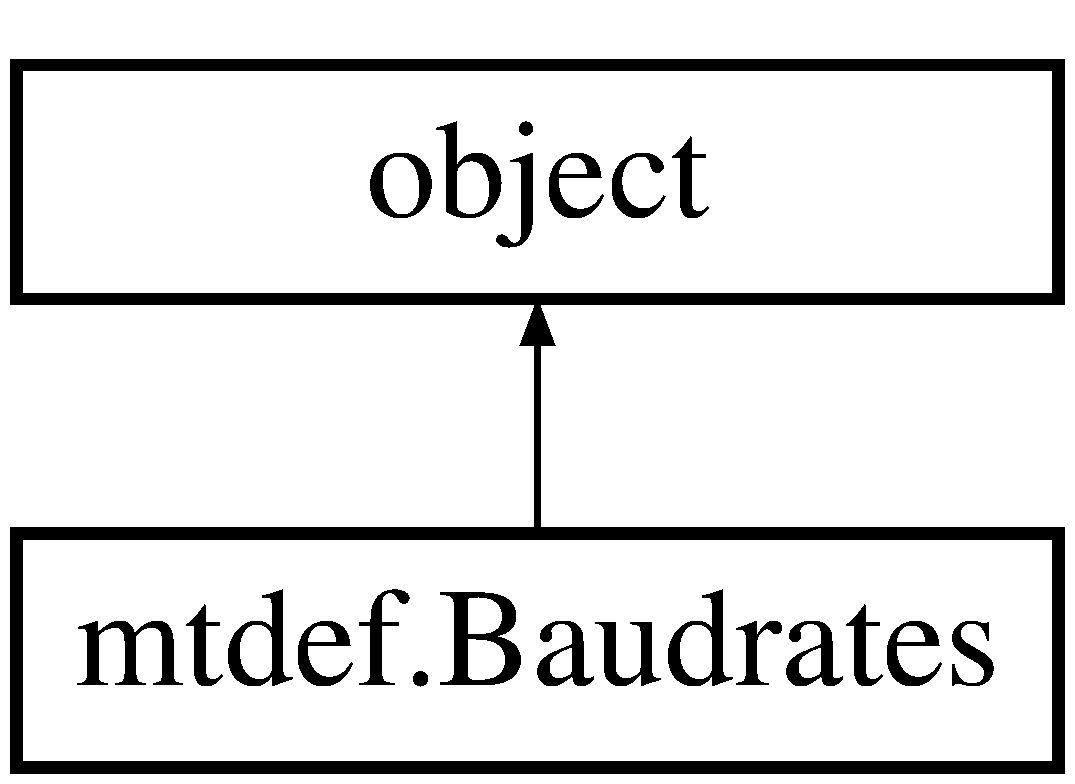
\includegraphics[height=2.000000cm]{classmtdef_1_1Baudrates}
\end{center}
\end{figure}
\doxysubsection*{Public Member Functions}
\begin{DoxyCompactItemize}
\item 
def \mbox{\hyperlink{classmtdef_1_1Baudrates_a32406f03907e8933f4216099b7a657a1}{get\+\_\+\+B\+R\+ID}} (cls, baudrate)
\item 
def \mbox{\hyperlink{classmtdef_1_1Baudrates_a9dff0be3c3e3dac46345f45e1f3fd481}{get\+\_\+\+BR}} (cls, baudrate\+\_\+id)
\end{DoxyCompactItemize}


\doxysubsection{Detailed Description}
\begin{DoxyVerb}Baudrate information and conversion.\end{DoxyVerb}
 

\doxysubsection{Member Function Documentation}
\mbox{\Hypertarget{classmtdef_1_1Baudrates_a9dff0be3c3e3dac46345f45e1f3fd481}\label{classmtdef_1_1Baudrates_a9dff0be3c3e3dac46345f45e1f3fd481}} 
\index{mtdef.Baudrates@{mtdef.Baudrates}!get\_BR@{get\_BR}}
\index{get\_BR@{get\_BR}!mtdef.Baudrates@{mtdef.Baudrates}}
\doxysubsubsection{\texorpdfstring{get\_BR()}{get\_BR()}}
{\footnotesize\ttfamily def mtdef.\+Baudrates.\+get\+\_\+\+BR (\begin{DoxyParamCaption}\item[{}]{cls,  }\item[{}]{baudrate\+\_\+id }\end{DoxyParamCaption})}

\begin{DoxyVerb}Get baudrate for a given baudrate id.\end{DoxyVerb}
 \mbox{\Hypertarget{classmtdef_1_1Baudrates_a32406f03907e8933f4216099b7a657a1}\label{classmtdef_1_1Baudrates_a32406f03907e8933f4216099b7a657a1}} 
\index{mtdef.Baudrates@{mtdef.Baudrates}!get\_BRID@{get\_BRID}}
\index{get\_BRID@{get\_BRID}!mtdef.Baudrates@{mtdef.Baudrates}}
\doxysubsubsection{\texorpdfstring{get\_BRID()}{get\_BRID()}}
{\footnotesize\ttfamily def mtdef.\+Baudrates.\+get\+\_\+\+B\+R\+ID (\begin{DoxyParamCaption}\item[{}]{cls,  }\item[{}]{baudrate }\end{DoxyParamCaption})}

\begin{DoxyVerb}Get baudrate id for a given baudrate.\end{DoxyVerb}
 

\doxysubsection{Member Data Documentation}
\mbox{\Hypertarget{classmtdef_1_1Baudrates_ad5d0122a011d49af285f6c1d94f11f8d}\label{classmtdef_1_1Baudrates_ad5d0122a011d49af285f6c1d94f11f8d}} 
\index{mtdef.Baudrates@{mtdef.Baudrates}!Baudrates@{Baudrates}}
\index{Baudrates@{Baudrates}!mtdef.Baudrates@{mtdef.Baudrates}}
\doxysubsubsection{\texorpdfstring{Baudrates}{Baudrates}}
{\footnotesize\ttfamily list mtdef.\+Baudrates.\+Baudrates\hspace{0.3cm}{\ttfamily [static]}}

{\bfseries Initial value\+:}
\begin{DoxyCode}{0}
\DoxyCodeLine{=  [}
\DoxyCodeLine{        (0x80, 921600),}
\DoxyCodeLine{        (0x0A, 921600),}
\DoxyCodeLine{        (0x00, 460800),}
\DoxyCodeLine{        (0x01, 230400),}
\DoxyCodeLine{        (0x02, 115200),}
\DoxyCodeLine{        (0x03,  76800),}
\DoxyCodeLine{        (0x04,  57600),}
\DoxyCodeLine{        (0x05,  38400),}
\DoxyCodeLine{        (0x06,  28800),}
\DoxyCodeLine{        (0x07,  19200),}
\DoxyCodeLine{        (0x08,  14400),}
\DoxyCodeLine{        (0x09,   9600),}
\DoxyCodeLine{        (0x0B,   4800),}
\DoxyCodeLine{        (0x80, 921600)]}

\end{DoxyCode}


The documentation for this class was generated from the following file\+:\begin{DoxyCompactItemize}
\item 
hardware\+\_\+layer/xsens\+\_\+driver/nodes/mtdef.\+py\end{DoxyCompactItemize}

\hypertarget{classuuv__trajectory__generator_1_1path__generator_1_1bezier__curve_1_1BezierCurve}{}\doxysection{uuv\+\_\+trajectory\+\_\+generator.\+path\+\_\+generator.\+bezier\+\_\+curve.\+Bezier\+Curve Class Reference}
\label{classuuv__trajectory__generator_1_1path__generator_1_1bezier__curve_1_1BezierCurve}\index{uuv\_trajectory\_generator.path\_generator.bezier\_curve.BezierCurve@{uuv\_trajectory\_generator.path\_generator.bezier\_curve.BezierCurve}}
Inheritance diagram for uuv\+\_\+trajectory\+\_\+generator.\+path\+\_\+generator.\+bezier\+\_\+curve.\+Bezier\+Curve\+:\begin{figure}[H]
\begin{center}
\leavevmode
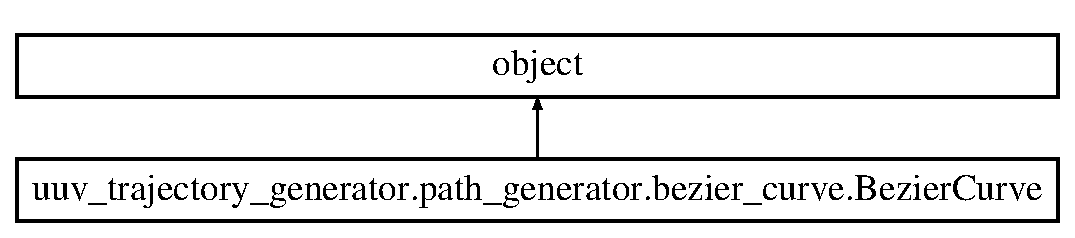
\includegraphics[height=2.000000cm]{classuuv__trajectory__generator_1_1path__generator_1_1bezier__curve_1_1BezierCurve}
\end{center}
\end{figure}
\doxysubsection*{Public Member Functions}
\begin{DoxyCompactItemize}
\item 
\mbox{\Hypertarget{classuuv__trajectory__generator_1_1path__generator_1_1bezier__curve_1_1BezierCurve_aec9ae9def8c2af614061e4dd48dbead5}\label{classuuv__trajectory__generator_1_1path__generator_1_1bezier__curve_1_1BezierCurve_aec9ae9def8c2af614061e4dd48dbead5}} 
def {\bfseries \+\_\+\+\_\+init\+\_\+\+\_\+} (self, pnts, order, tangents=None, normals=None)
\item 
\mbox{\Hypertarget{classuuv__trajectory__generator_1_1path__generator_1_1bezier__curve_1_1BezierCurve_a304cf7918064949b61e43213ae872565}\label{classuuv__trajectory__generator_1_1path__generator_1_1bezier__curve_1_1BezierCurve_a304cf7918064949b61e43213ae872565}} 
def {\bfseries control\+\_\+pnts} (self)
\item 
\mbox{\Hypertarget{classuuv__trajectory__generator_1_1path__generator_1_1bezier__curve_1_1BezierCurve_a821630c0eb9cbd45ef9a3befcaf34e9d}\label{classuuv__trajectory__generator_1_1path__generator_1_1bezier__curve_1_1BezierCurve_a821630c0eb9cbd45ef9a3befcaf34e9d}} 
def {\bfseries interpolate} (self, u)
\item 
\mbox{\Hypertarget{classuuv__trajectory__generator_1_1path__generator_1_1bezier__curve_1_1BezierCurve_ab509016f03e7d5b4585e61538a9e4385}\label{classuuv__trajectory__generator_1_1path__generator_1_1bezier__curve_1_1BezierCurve_ab509016f03e7d5b4585e61538a9e4385}} 
def {\bfseries get\+\_\+derivative} (self, u, order=1)
\item 
\mbox{\Hypertarget{classuuv__trajectory__generator_1_1path__generator_1_1bezier__curve_1_1BezierCurve_aef57d022474bb02e69cc5fd33c499a8a}\label{classuuv__trajectory__generator_1_1path__generator_1_1bezier__curve_1_1BezierCurve_aef57d022474bb02e69cc5fd33c499a8a}} 
def {\bfseries get\+\_\+length} (self)
\item 
\mbox{\Hypertarget{classuuv__trajectory__generator_1_1path__generator_1_1bezier__curve_1_1BezierCurve_a81849b78981df7c43f738821449e0ba3}\label{classuuv__trajectory__generator_1_1path__generator_1_1bezier__curve_1_1BezierCurve_a81849b78981df7c43f738821449e0ba3}} 
def {\bfseries compute\+\_\+polynomial} (self, n, i, u)
\end{DoxyCompactItemize}
\doxysubsection*{Static Public Member Functions}
\begin{DoxyCompactItemize}
\item 
\mbox{\Hypertarget{classuuv__trajectory__generator_1_1path__generator_1_1bezier__curve_1_1BezierCurve_a772bef89a3b771066af31c5f0eba2b20}\label{classuuv__trajectory__generator_1_1path__generator_1_1bezier__curve_1_1BezierCurve_a772bef89a3b771066af31c5f0eba2b20}} 
def {\bfseries distance} (p1, p2)
\item 
\mbox{\Hypertarget{classuuv__trajectory__generator_1_1path__generator_1_1bezier__curve_1_1BezierCurve_a723a5887df791e2c89ca68b61f49ba45}\label{classuuv__trajectory__generator_1_1path__generator_1_1bezier__curve_1_1BezierCurve_a723a5887df791e2c89ca68b61f49ba45}} 
def {\bfseries generate\+\_\+cubic\+\_\+curve} (pnts)
\item 
\mbox{\Hypertarget{classuuv__trajectory__generator_1_1path__generator_1_1bezier__curve_1_1BezierCurve_ad7bf32a3ab998dc9db0aae120d9a5a67}\label{classuuv__trajectory__generator_1_1path__generator_1_1bezier__curve_1_1BezierCurve_ad7bf32a3ab998dc9db0aae120d9a5a67}} 
def {\bfseries generate\+\_\+quintic\+\_\+curve} (pnts)
\end{DoxyCompactItemize}


\doxysubsection{Detailed Description}
\begin{DoxyVerb}Implementation of Bezier curves of orders 3, 4 and 5 based on [1].

[1] Biagiotti, Luigi, and Claudio Melchiorri. Trajectory planning for 
    automatic machines and robots. Springer Science & Business Media, 2008.
\end{DoxyVerb}
 

The documentation for this class was generated from the following file\+:\begin{DoxyCompactItemize}
\item 
control\+\_\+layer/uuv\+\_\+trajectory\+\_\+control/src/uuv\+\_\+trajectory\+\_\+generator/path\+\_\+generator/bezier\+\_\+curve.\+py\end{DoxyCompactItemize}

\hypertarget{classmaster__layer_1_1state__mach__gate__torpedo_1_1BouyTask}{}\section{master\+\_\+layer.\+state\+\_\+mach\+\_\+gate\+\_\+torpedo.\+Bouy\+Task Class Reference}
\label{classmaster__layer_1_1state__mach__gate__torpedo_1_1BouyTask}\index{master\+\_\+layer.\+state\+\_\+mach\+\_\+gate\+\_\+torpedo.\+Bouy\+Task@{master\+\_\+layer.\+state\+\_\+mach\+\_\+gate\+\_\+torpedo.\+Bouy\+Task}}
Inheritance diagram for master\+\_\+layer.\+state\+\_\+mach\+\_\+gate\+\_\+torpedo.\+Bouy\+Task\+:\begin{figure}[H]
\begin{center}
\leavevmode
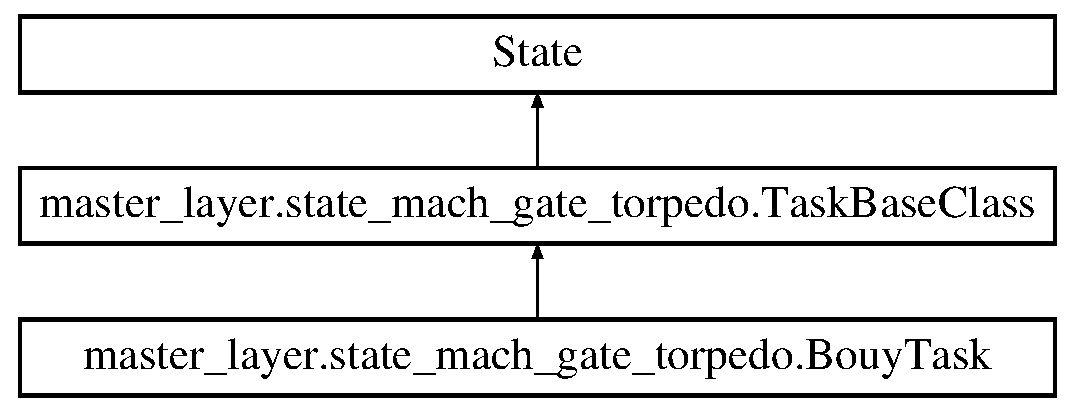
\includegraphics[height=3.000000cm]{classmaster__layer_1_1state__mach__gate__torpedo_1_1BouyTask}
\end{center}
\end{figure}
\subsection*{Public Member Functions}
\begin{DoxyCompactItemize}
\item 
\mbox{\Hypertarget{classmaster__layer_1_1state__mach__gate__torpedo_1_1BouyTask_aba070e4fb4114ba76e4fcf7487bd3f71}\label{classmaster__layer_1_1state__mach__gate__torpedo_1_1BouyTask_aba070e4fb4114ba76e4fcf7487bd3f71}} 
def {\bfseries \+\_\+\+\_\+init\+\_\+\+\_\+} (self)
\item 
\mbox{\Hypertarget{classmaster__layer_1_1state__mach__gate__torpedo_1_1BouyTask_aad1969a3203424015b3884640e75ff3a}\label{classmaster__layer_1_1state__mach__gate__torpedo_1_1BouyTask_aad1969a3203424015b3884640e75ff3a}} 
def {\bfseries hit\+\_\+buoy} (self)
\item 
\mbox{\Hypertarget{classmaster__layer_1_1state__mach__gate__torpedo_1_1BouyTask_a2bdf8018611fc160803f144ade19b80c}\label{classmaster__layer_1_1state__mach__gate__torpedo_1_1BouyTask_a2bdf8018611fc160803f144ade19b80c}} 
def {\bfseries get\+\_\+back} (self)
\item 
\mbox{\Hypertarget{classmaster__layer_1_1state__mach__gate__torpedo_1_1BouyTask_a661817de7db221031d14d5c153ad8c6b}\label{classmaster__layer_1_1state__mach__gate__torpedo_1_1BouyTask_a661817de7db221031d14d5c153ad8c6b}} 
def {\bfseries execute} (self)
\end{DoxyCompactItemize}


The documentation for this class was generated from the following file\+:\begin{DoxyCompactItemize}
\item 
master\+\_\+layer/src/master\+\_\+layer/state\+\_\+mach\+\_\+gate\+\_\+torpedo.\+py\end{DoxyCompactItemize}

\hypertarget{classmaster__layer_1_1state__mach_1_1BouyTask}{}\doxysection{master\+\_\+layer.\+state\+\_\+mach.\+Bouy\+Task Class Reference}
\label{classmaster__layer_1_1state__mach_1_1BouyTask}\index{master\_layer.state\_mach.BouyTask@{master\_layer.state\_mach.BouyTask}}
Inheritance diagram for master\+\_\+layer.\+state\+\_\+mach.\+Bouy\+Task\+:\begin{figure}[H]
\begin{center}
\leavevmode
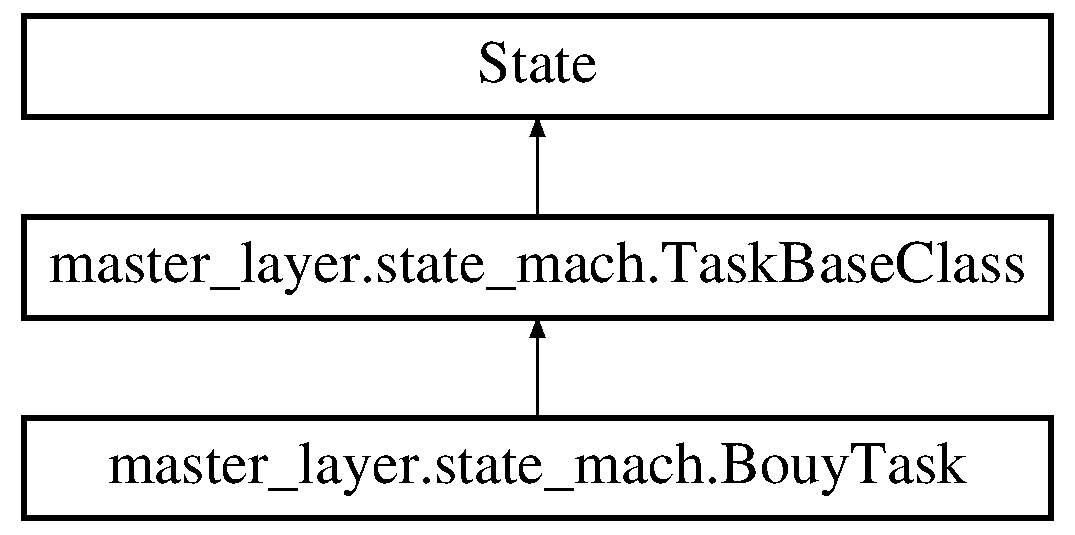
\includegraphics[height=3.000000cm]{classmaster__layer_1_1state__mach_1_1BouyTask}
\end{center}
\end{figure}
\doxysubsection*{Public Member Functions}
\begin{DoxyCompactItemize}
\item 
\mbox{\Hypertarget{classmaster__layer_1_1state__mach_1_1BouyTask_a7ddfda8c598ac1e21a7c4649069fe4e5}\label{classmaster__layer_1_1state__mach_1_1BouyTask_a7ddfda8c598ac1e21a7c4649069fe4e5}} 
def {\bfseries \+\_\+\+\_\+init\+\_\+\+\_\+} (self)
\item 
\mbox{\Hypertarget{classmaster__layer_1_1state__mach_1_1BouyTask_a45dad7f836ef16473a903f3ffc7c3b78}\label{classmaster__layer_1_1state__mach_1_1BouyTask_a45dad7f836ef16473a903f3ffc7c3b78}} 
def {\bfseries hit\+\_\+buoy} (self)
\item 
\mbox{\Hypertarget{classmaster__layer_1_1state__mach_1_1BouyTask_a3b587fc85248bf49f6ebee0dd1643025}\label{classmaster__layer_1_1state__mach_1_1BouyTask_a3b587fc85248bf49f6ebee0dd1643025}} 
def {\bfseries get\+\_\+back} (self)
\item 
\mbox{\Hypertarget{classmaster__layer_1_1state__mach_1_1BouyTask_a94dd3606491b6e86a60fa2ec02e6a295}\label{classmaster__layer_1_1state__mach_1_1BouyTask_a94dd3606491b6e86a60fa2ec02e6a295}} 
def {\bfseries execute} (self)
\end{DoxyCompactItemize}


The documentation for this class was generated from the following file\+:\begin{DoxyCompactItemize}
\item 
master\+\_\+layer/src/master\+\_\+layer/state\+\_\+mach.\+py\end{DoxyCompactItemize}

\hypertarget{classBuoy}{}\section{Buoy Class Reference}
\label{classBuoy}\index{Buoy@{Buoy}}
Inheritance diagram for Buoy\+:\begin{figure}[H]
\begin{center}
\leavevmode
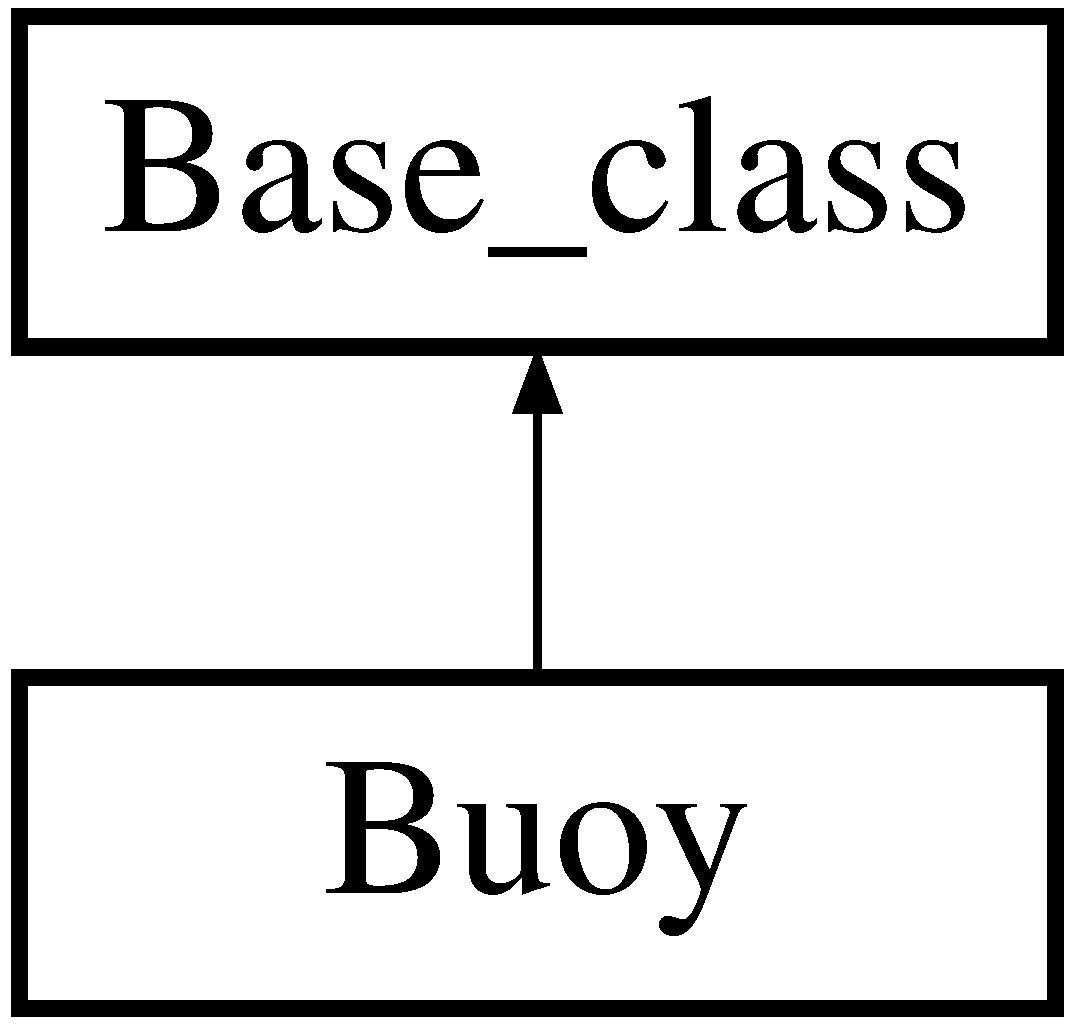
\includegraphics[height=2.000000cm]{classBuoy}
\end{center}
\end{figure}
\subsection*{Public Member Functions}
\begin{DoxyCompactItemize}
\item 
\mbox{\Hypertarget{classBuoy_aae6a7d935b45ae2d5aa10aa80d46e0d7}\label{classBuoy_aae6a7d935b45ae2d5aa10aa80d46e0d7}} 
void {\bfseries switch\+Color} (int)
\item 
\mbox{\Hypertarget{classBuoy_ae24b8d548c1f922122020c23d53c190b}\label{classBuoy_ae24b8d548c1f922122020c23d53c190b}} 
void {\bfseries spin\+Thread\+Front} ()
\item 
\mbox{\Hypertarget{classBuoy_a787135abf00b8fff3e3cf96ccc9ba0ec}\label{classBuoy_a787135abf00b8fff3e3cf96ccc9ba0ec}} 
void {\bfseries spin\+Thread} ()
\end{DoxyCompactItemize}
\subsection*{Public Attributes}
\begin{DoxyCompactItemize}
\item 
\mbox{\Hypertarget{classBuoy_a52630f83ade22809208e0050fd189bb0}\label{classBuoy_a52630f83ade22809208e0050fd189bb0}} 
int {\bfseries current\+\_\+color}
\end{DoxyCompactItemize}
\subsection*{Protected Member Functions}
\begin{DoxyCompactItemize}
\item 
\mbox{\Hypertarget{classBuoy_a7dde14ad16d6eae2612687a41d8a466c}\label{classBuoy_a7dde14ad16d6eae2612687a41d8a466c}} 
void {\bfseries callback} (vision\+\_\+tasks\+::buoy\+Range\+Config \&config, double level)
\item 
\mbox{\Hypertarget{classBuoy_add99f142a60bce53abe8cb6c6e224933}\label{classBuoy_add99f142a60bce53abe8cb6c6e224933}} 
void {\bfseries image\+Callback} (const sensor\+\_\+msgs\+::\+Image\+::\+Const\+Ptr \&msg)
\end{DoxyCompactItemize}
\subsection*{Protected Attributes}
\begin{DoxyCompactItemize}
\item 
\mbox{\Hypertarget{classBuoy_ad94fe9e5a32dfbffbf5538277b28e809}\label{classBuoy_ad94fe9e5a32dfbffbf5538277b28e809}} 
ros\+::\+Node\+Handle {\bfseries nh}
\item 
\mbox{\Hypertarget{classBuoy_a391e658428c21fa5d7af57cd7a3fc664}\label{classBuoy_a391e658428c21fa5d7af57cd7a3fc664}} 
image\+\_\+transport\+::\+Publisher {\bfseries blue\+\_\+filtered\+\_\+pub}
\item 
\mbox{\Hypertarget{classBuoy_a1f023c4f4e8e92e97babd731d19c5901}\label{classBuoy_a1f023c4f4e8e92e97babd731d19c5901}} 
image\+\_\+transport\+::\+Subscriber {\bfseries image\+\_\+raw\+\_\+sub}
\item 
\mbox{\Hypertarget{classBuoy_ad8a61f22312a2af443d491f6d8a95c88}\label{classBuoy_ad8a61f22312a2af443d491f6d8a95c88}} 
std\+::string {\bfseries camera\+\_\+frame\+\_\+}
\item 
\mbox{\Hypertarget{classBuoy_a832c660d31a540d9fcc17c7f3d8f68d8}\label{classBuoy_a832c660d31a540d9fcc17c7f3d8f68d8}} 
double {\bfseries clahe\+\_\+clip\+\_\+}
\item 
\mbox{\Hypertarget{classBuoy_aa47cb1503c015132f210dfc713749a72}\label{classBuoy_aa47cb1503c015132f210dfc713749a72}} 
int {\bfseries clahe\+\_\+grid\+\_\+size\+\_\+}
\item 
\mbox{\Hypertarget{classBuoy_aca1a7c7645c39831707746a8b9bb6992}\label{classBuoy_aca1a7c7645c39831707746a8b9bb6992}} 
int {\bfseries clahe\+\_\+bilateral\+\_\+iter\+\_\+}
\item 
\mbox{\Hypertarget{classBuoy_a76c480b4d7d16f9ec58a50d99c64a46e}\label{classBuoy_a76c480b4d7d16f9ec58a50d99c64a46e}} 
int {\bfseries balanced\+\_\+bilateral\+\_\+iter\+\_\+}
\item 
\mbox{\Hypertarget{classBuoy_ab6587d9953014573ed5b89aebb989d61}\label{classBuoy_ab6587d9953014573ed5b89aebb989d61}} 
double {\bfseries denoise\+\_\+h\+\_\+}
\item 
\mbox{\Hypertarget{classBuoy_a481fc15e25346fd346a14f2bff84a55f}\label{classBuoy_a481fc15e25346fd346a14f2bff84a55f}} 
int {\bfseries data\+\_\+low\+\_\+h} \mbox{[}3\mbox{]} = \{0, 12, 0\}
\item 
\mbox{\Hypertarget{classBuoy_aabf668782fb78cd57c57935f5556f9a7}\label{classBuoy_aabf668782fb78cd57c57935f5556f9a7}} 
int {\bfseries data\+\_\+high\+\_\+h} \mbox{[}3\mbox{]} = \{17, 40, 56\}
\item 
\mbox{\Hypertarget{classBuoy_a46d4f0a04d9eec9f40086ced3e674679}\label{classBuoy_a46d4f0a04d9eec9f40086ced3e674679}} 
int {\bfseries data\+\_\+low\+\_\+s} \mbox{[}3\mbox{]} = \{206, 183, 0\}
\item 
\mbox{\Hypertarget{classBuoy_a488a83dc51aadd7ffc5f02e08f27728e}\label{classBuoy_a488a83dc51aadd7ffc5f02e08f27728e}} 
int {\bfseries data\+\_\+high\+\_\+s} \mbox{[}3\mbox{]} = \{255, 255, 255\}
\item 
\mbox{\Hypertarget{classBuoy_aea30660a61beb8dbff66ae13d8851bf9}\label{classBuoy_aea30660a61beb8dbff66ae13d8851bf9}} 
int {\bfseries data\+\_\+low\+\_\+v} \mbox{[}3\mbox{]} = \{30, 3, 2\}
\item 
\mbox{\Hypertarget{classBuoy_a8ec5f9ef0ebb0ddf8497d89b99f80b1c}\label{classBuoy_a8ec5f9ef0ebb0ddf8497d89b99f80b1c}} 
int {\bfseries data\+\_\+high\+\_\+v} \mbox{[}3\mbox{]} = \{255, 255, 82\}
\end{DoxyCompactItemize}


The documentation for this class was generated from the following files\+:\begin{DoxyCompactItemize}
\item 
vision\+\_\+layer/vision\+\_\+tasks/include/buoy.\+h\item 
vision\+\_\+layer/vision\+\_\+tasks/src/buoy.\+cpp\end{DoxyCompactItemize}

\hypertarget{classimage__undistort_1_1CameraParametersPair}{}\section{image\+\_\+undistort\+:\+:Camera\+Parameters\+Pair Class Reference}
\label{classimage__undistort_1_1CameraParametersPair}\index{image\+\_\+undistort\+::\+Camera\+Parameters\+Pair@{image\+\_\+undistort\+::\+Camera\+Parameters\+Pair}}
\subsection*{Public Member Functions}
\begin{DoxyCompactItemize}
\item 
\mbox{\Hypertarget{classimage__undistort_1_1CameraParametersPair_ad4261cd5f63ee7f798bfce0e348e9070}\label{classimage__undistort_1_1CameraParametersPair_ad4261cd5f63ee7f798bfce0e348e9070}} 
{\bfseries Camera\+Parameters\+Pair} (const Distortion\+Processing distortion\+\_\+processing=Distortion\+Processing\+::\+U\+N\+D\+I\+S\+T\+O\+RT)
\item 
\mbox{\Hypertarget{classimage__undistort_1_1CameraParametersPair_ae80f2f5b17cceb4c2584578bc1045ea1}\label{classimage__undistort_1_1CameraParametersPair_ae80f2f5b17cceb4c2584578bc1045ea1}} 
bool {\bfseries set\+Camera\+Parameters} (const ros\+::\+Node\+Handle \&nh, const std\+::string \&camera\+\_\+namespace, const Camera\+IO \&io, const bool invert\+\_\+T=false)
\item 
\mbox{\Hypertarget{classimage__undistort_1_1CameraParametersPair_a1984650bd098e6081d45f68ac59fcacb}\label{classimage__undistort_1_1CameraParametersPair_a1984650bd098e6081d45f68ac59fcacb}} 
bool {\bfseries set\+Camera\+Parameters} (const sensor\+\_\+msgs\+::\+Camera\+Info \&camera\+\_\+info, const Camera\+IO \&io)
\item 
\mbox{\Hypertarget{classimage__undistort_1_1CameraParametersPair_a3f7b17993f586f0a3862b48622f5e274}\label{classimage__undistort_1_1CameraParametersPair_a3f7b17993f586f0a3862b48622f5e274}} 
bool {\bfseries set\+Input\+Camera\+Parameters} (const cv\+::\+Size \&resolution, const Eigen\+::\+Matrix$<$ double, 4, 4 $>$ \&T, const Eigen\+::\+Matrix$<$ double, 3, 3 $>$ \&K, const std\+::vector$<$ double $>$ \&D, const Distortion\+Model \&distortion\+\_\+model)
\item 
\mbox{\Hypertarget{classimage__undistort_1_1CameraParametersPair_a69fbca3593a0dca84fa098cfbb767f78}\label{classimage__undistort_1_1CameraParametersPair_a69fbca3593a0dca84fa098cfbb767f78}} 
bool {\bfseries set\+Output\+Camera\+Parameters} (const cv\+::\+Size \&resolution, const Eigen\+::\+Matrix$<$ double, 4, 4 $>$ \&T, const Eigen\+::\+Matrix$<$ double, 3, 3 $>$ \&K)
\item 
\mbox{\Hypertarget{classimage__undistort_1_1CameraParametersPair_a76f1696eb8e468dc26f9cd60893d1eca}\label{classimage__undistort_1_1CameraParametersPair_a76f1696eb8e468dc26f9cd60893d1eca}} 
bool {\bfseries set\+Output\+From\+Input} (const double scale)
\item 
\mbox{\Hypertarget{classimage__undistort_1_1CameraParametersPair_ab1392597334cbe8286cbc1903b197d5f}\label{classimage__undistort_1_1CameraParametersPair_ab1392597334cbe8286cbc1903b197d5f}} 
bool {\bfseries set\+Optimal\+Output\+Camera\+Parameters} (const double scale)
\item 
\mbox{\Hypertarget{classimage__undistort_1_1CameraParametersPair_ad54793186833d6a8b8f5834f73305b40}\label{classimage__undistort_1_1CameraParametersPair_ad54793186833d6a8b8f5834f73305b40}} 
const Distortion\+Processing \& {\bfseries distortion\+Processing} () const
\item 
\mbox{\Hypertarget{classimage__undistort_1_1CameraParametersPair_a5dc61d00a297a78d2be1bc49eace3736}\label{classimage__undistort_1_1CameraParametersPair_a5dc61d00a297a78d2be1bc49eace3736}} 
void {\bfseries generate\+Camera\+Info\+Message} (const Camera\+IO \&io, sensor\+\_\+msgs\+::\+Camera\+Info $\ast$camera\+\_\+info) const
\item 
\mbox{\Hypertarget{classimage__undistort_1_1CameraParametersPair_ac874db6136c57afb3ab30e818d501975}\label{classimage__undistort_1_1CameraParametersPair_ac874db6136c57afb3ab30e818d501975}} 
const std\+::shared\+\_\+ptr$<$ \hyperlink{classimage__undistort_1_1InputCameraParameters}{Input\+Camera\+Parameters} $>$ \& {\bfseries get\+Input\+Ptr} () const
\item 
\mbox{\Hypertarget{classimage__undistort_1_1CameraParametersPair_ac9d8e14065c1e8b98eecaea4a209253e}\label{classimage__undistort_1_1CameraParametersPair_ac9d8e14065c1e8b98eecaea4a209253e}} 
const std\+::shared\+\_\+ptr$<$ \hyperlink{classimage__undistort_1_1OutputCameraParameters}{Output\+Camera\+Parameters} $>$ \& {\bfseries get\+Output\+Ptr} () const
\item 
\mbox{\Hypertarget{classimage__undistort_1_1CameraParametersPair_a11bd354b0961ecf37939dcc9668c9e69}\label{classimage__undistort_1_1CameraParametersPair_a11bd354b0961ecf37939dcc9668c9e69}} 
bool {\bfseries valid} () const
\item 
\mbox{\Hypertarget{classimage__undistort_1_1CameraParametersPair_ab80fb96d3419762f23a6f10a67e848c7}\label{classimage__undistort_1_1CameraParametersPair_ab80fb96d3419762f23a6f10a67e848c7}} 
bool {\bfseries valid} (const Camera\+IO \&io) const
\item 
\mbox{\Hypertarget{classimage__undistort_1_1CameraParametersPair_a8eca6daae8442e95a6612f76543a1de9}\label{classimage__undistort_1_1CameraParametersPair_a8eca6daae8442e95a6612f76543a1de9}} 
bool {\bfseries operator==} (const \hyperlink{classimage__undistort_1_1CameraParametersPair}{Camera\+Parameters\+Pair} \&B) const
\item 
\mbox{\Hypertarget{classimage__undistort_1_1CameraParametersPair_a1e905f613d6a26a8a0f816e2aff61496}\label{classimage__undistort_1_1CameraParametersPair_a1e905f613d6a26a8a0f816e2aff61496}} 
bool {\bfseries operator!=} (const \hyperlink{classimage__undistort_1_1CameraParametersPair}{Camera\+Parameters\+Pair} \&B) const
\end{DoxyCompactItemize}


The documentation for this class was generated from the following files\+:\begin{DoxyCompactItemize}
\item 
vision\+\_\+layer/image\+\_\+undistort/include/image\+\_\+undistort/camera\+\_\+parameters.\+h\item 
vision\+\_\+layer/image\+\_\+undistort/src/camera\+\_\+parameters.\+cpp\end{DoxyCompactItemize}

\hypertarget{classcolor__correction}{}\doxysection{color\+\_\+correction Class Reference}
\label{classcolor__correction}\index{color\_correction@{color\_correction}}


class defining generic interfaces and methods common for color correction methods  




{\ttfamily \#include $<$color\+\_\+constancy.\+hpp$>$}

\doxysubsection*{Classes}
\begin{DoxyCompactItemize}
\item 
class \mbox{\hyperlink{classcolor__correction_1_1contrast__stretching}{contrast\+\_\+stretching}}
\begin{DoxyCompactList}\small\item\em class defining methods to perform color correction using modified contrast stretching \end{DoxyCompactList}\item 
class \mbox{\hyperlink{classcolor__correction_1_1gray__edge}{gray\+\_\+edge}}
\item 
class \mbox{\hyperlink{classcolor__correction_1_1gray__world}{gray\+\_\+world}}
\item 
class \mbox{\hyperlink{classcolor__correction_1_1max__edge}{max\+\_\+edge}}
\item 
class \mbox{\hyperlink{classcolor__correction_1_1maxRGB}{max\+R\+GB}}
\end{DoxyCompactItemize}


\doxysubsection{Detailed Description}
class defining generic interfaces and methods common for color correction methods 

The documentation for this class was generated from the following file\+:\begin{DoxyCompactItemize}
\item 
vision\+\_\+layer/vision\+\_\+fusion/include/fusion/color\+\_\+constancy.\+hpp\end{DoxyCompactItemize}

\hypertarget{classvision__commons_1_1Contour}{}\section{vision\+\_\+commons\+:\+:Contour Class Reference}
\label{classvision__commons_1_1Contour}\index{vision\+\_\+commons\+::\+Contour@{vision\+\_\+commons\+::\+Contour}}
\subsection*{Static Public Member Functions}
\begin{DoxyCompactItemize}
\item 
\mbox{\Hypertarget{classvision__commons_1_1Contour_afbf0efa9f03f40eb38f3b889262e8284}\label{classvision__commons_1_1Contour_afbf0efa9f03f40eb38f3b889262e8284}} 
static std\+::vector$<$ std\+::vector$<$ cv\+::\+Point $>$ $>$ {\bfseries get\+BestX} (cv\+::\+Mat \&raw, int x)
\item 
\mbox{\Hypertarget{classvision__commons_1_1Contour_a194702cb0e126c5d006b3a63b755fdc8}\label{classvision__commons_1_1Contour_a194702cb0e126c5d006b3a63b755fdc8}} 
static std\+::vector$<$ std\+::vector$<$ cv\+::\+Point $>$ $>$ {\bfseries get\+Best\+X\+Convex\+Hulled} (cv\+::\+Mat \&raw, int x)
\item 
\mbox{\Hypertarget{classvision__commons_1_1Contour_a58ce1db921cc4e834038de296d0fad6a}\label{classvision__commons_1_1Contour_a58ce1db921cc4e834038de296d0fad6a}} 
static std\+::vector$<$ cv\+::\+Point $>$ {\bfseries get\+Largest\+Contour} (cv\+::\+Mat \&raw)
\item 
\mbox{\Hypertarget{classvision__commons_1_1Contour_a71b6dd8585b3a0113f121b79aea43cfa}\label{classvision__commons_1_1Contour_a71b6dd8585b3a0113f121b79aea43cfa}} 
static void {\bfseries filter\+Contours} (const std\+::vector$<$ std\+::vector$<$ cv\+::\+Point $>$ $>$ \&contours, std\+::vector$<$ int $>$ \&idx, double threshold)
\item 
\mbox{\Hypertarget{classvision__commons_1_1Contour_a4925cbaeffe176f452546194009079f0}\label{classvision__commons_1_1Contour_a4925cbaeffe176f452546194009079f0}} 
static std\+::vector$<$ std\+::vector$<$ cv\+::\+Point $>$ $>$ {\bfseries filter\+Contours} (const std\+::vector$<$ std\+::vector$<$ cv\+::\+Point $>$ $>$ \&contours, double threshold)
\item 
\mbox{\Hypertarget{classvision__commons_1_1Contour_a83cc11df062249a286aa0390ed3c6b7c}\label{classvision__commons_1_1Contour_a83cc11df062249a286aa0390ed3c6b7c}} 
static void {\bfseries sort\+From\+Big\+To\+Small} (std\+::vector$<$ std\+::vector$<$ cv\+::\+Point $>$ $>$ \&contours)
\end{DoxyCompactItemize}


The documentation for this class was generated from the following files\+:\begin{DoxyCompactItemize}
\item 
vision\+\_\+layer/vision\+\_\+commons/include/contour.\+h\item 
vision\+\_\+layer/vision\+\_\+commons/src/contour.\+cpp\end{DoxyCompactItemize}

\hypertarget{classcolor__correction_1_1contrast__stretching}{}\doxysection{color\+\_\+correction\+::contrast\+\_\+stretching Class Reference}
\label{classcolor__correction_1_1contrast__stretching}\index{color\_correction::contrast\_stretching@{color\_correction::contrast\_stretching}}


class defining methods to perform color correction using modified contrast stretching  




{\ttfamily \#include $<$color\+\_\+constancy.\+hpp$>$}

\doxysubsection*{Public Member Functions}
\begin{DoxyCompactItemize}
\item 
Mat \mbox{\hyperlink{classcolor__correction_1_1contrast__stretching_a034f45ac1d117193c70e87104a2ee82c}{run}} (Mat)
\item 
Mat \mbox{\hyperlink{classcolor__correction_1_1contrast__stretching_a059efe3142744d161a0022ffeff5b79c}{run1}} (Mat src)
\end{DoxyCompactItemize}


\doxysubsection{Detailed Description}
class defining methods to perform color correction using modified contrast stretching 

\doxysubsection{Member Function Documentation}
\mbox{\Hypertarget{classcolor__correction_1_1contrast__stretching_a034f45ac1d117193c70e87104a2ee82c}\label{classcolor__correction_1_1contrast__stretching_a034f45ac1d117193c70e87104a2ee82c}} 
\index{color\_correction::contrast\_stretching@{color\_correction::contrast\_stretching}!run@{run}}
\index{run@{run}!color\_correction::contrast\_stretching@{color\_correction::contrast\_stretching}}
\doxysubsubsection{\texorpdfstring{run()}{run()}}
{\footnotesize\ttfamily Mat color\+\_\+correction\+::contrast\+\_\+stretching\+::run (\begin{DoxyParamCaption}\item[{Mat}]{src }\end{DoxyParamCaption})}

The main method called to perform color correction using modified contrast stretching The only input required is the input image The method computes the lower and higher threshold pixel values and then calls the \mbox{\hyperlink{classcolor__correction_1_1contrast__stretching}{contrast\+\_\+stretching}} method \mbox{\Hypertarget{classcolor__correction_1_1contrast__stretching_a059efe3142744d161a0022ffeff5b79c}\label{classcolor__correction_1_1contrast__stretching_a059efe3142744d161a0022ffeff5b79c}} 
\index{color\_correction::contrast\_stretching@{color\_correction::contrast\_stretching}!run1@{run1}}
\index{run1@{run1}!color\_correction::contrast\_stretching@{color\_correction::contrast\_stretching}}
\doxysubsubsection{\texorpdfstring{run1()}{run1()}}
{\footnotesize\ttfamily Mat color\+\_\+correction\+::contrast\+\_\+stretching\+::run1 (\begin{DoxyParamCaption}\item[{Mat}]{src }\end{DoxyParamCaption})}

Establish the number of bins

Set the ranges ( for B,G,R) )

The documentation for this class was generated from the following files\+:\begin{DoxyCompactItemize}
\item 
vision\+\_\+layer/vision\+\_\+fusion/include/fusion/color\+\_\+constancy.\+hpp\item 
vision\+\_\+layer/vision\+\_\+fusion/src/color\+\_\+constancy.\+cpp\end{DoxyCompactItemize}

\hypertarget{classCrucifix}{}\doxysection{Crucifix Class Reference}
\label{classCrucifix}\index{Crucifix@{Crucifix}}
Inheritance diagram for Crucifix\+:\begin{figure}[H]
\begin{center}
\leavevmode
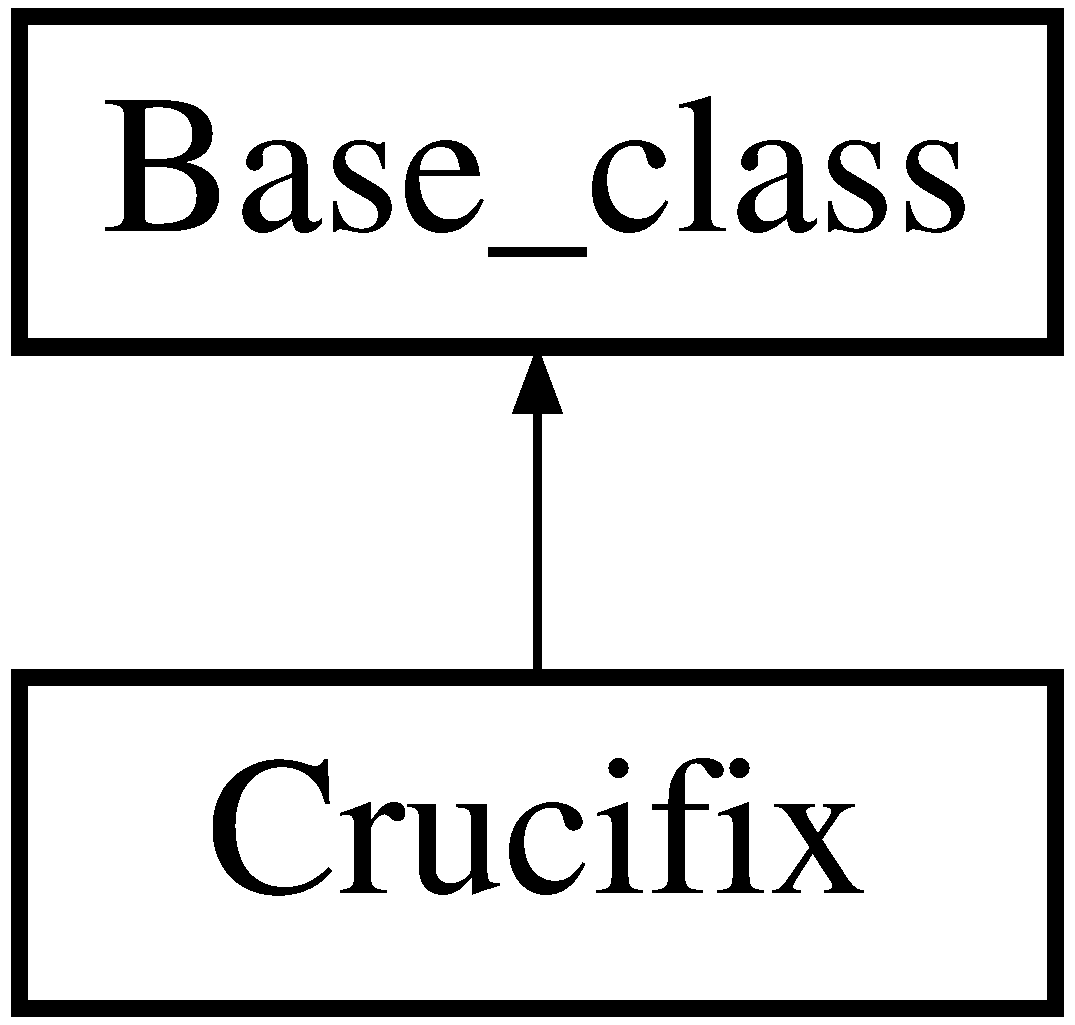
\includegraphics[height=2.000000cm]{classCrucifix}
\end{center}
\end{figure}
\doxysubsection*{Public Member Functions}
\begin{DoxyCompactItemize}
\item 
\mbox{\Hypertarget{classCrucifix_ae24529f27f24c27e7feb7032cf053a77}\label{classCrucifix_ae24529f27f24c27e7feb7032cf053a77}} 
virtual void {\bfseries load\+Params} () override
\item 
\mbox{\Hypertarget{classCrucifix_a0b540387c8f1ec0a35c72e9d5c2ca56b}\label{classCrucifix_a0b540387c8f1ec0a35c72e9d5c2ca56b}} 
virtual void {\bfseries spin\+Thread\+Front} () override
\item 
\mbox{\Hypertarget{classCrucifix_aa60e6db3bd7731a36b2ae166eb77f464}\label{classCrucifix_aa60e6db3bd7731a36b2ae166eb77f464}} 
virtual void {\bfseries spin\+Thread\+Bottom} () override
\end{DoxyCompactItemize}
\doxysubsection*{Additional Inherited Members}


The documentation for this class was generated from the following files\+:\begin{DoxyCompactItemize}
\item 
vision\+\_\+layer/vision\+\_\+tasks/include/crucifix.\+h\item 
vision\+\_\+layer/vision\+\_\+tasks/src/crucifix.\+cpp\end{DoxyCompactItemize}

\hypertarget{classuuv__trajectory__generator_1_1path__generator_1_1cs__interpolator_1_1CSInterpolator}{}\section{uuv\+\_\+trajectory\+\_\+generator.\+path\+\_\+generator.\+cs\+\_\+interpolator.\+C\+S\+Interpolator Class Reference}
\label{classuuv__trajectory__generator_1_1path__generator_1_1cs__interpolator_1_1CSInterpolator}\index{uuv\+\_\+trajectory\+\_\+generator.\+path\+\_\+generator.\+cs\+\_\+interpolator.\+C\+S\+Interpolator@{uuv\+\_\+trajectory\+\_\+generator.\+path\+\_\+generator.\+cs\+\_\+interpolator.\+C\+S\+Interpolator}}
Inheritance diagram for uuv\+\_\+trajectory\+\_\+generator.\+path\+\_\+generator.\+cs\+\_\+interpolator.\+C\+S\+Interpolator\+:\begin{figure}[H]
\begin{center}
\leavevmode
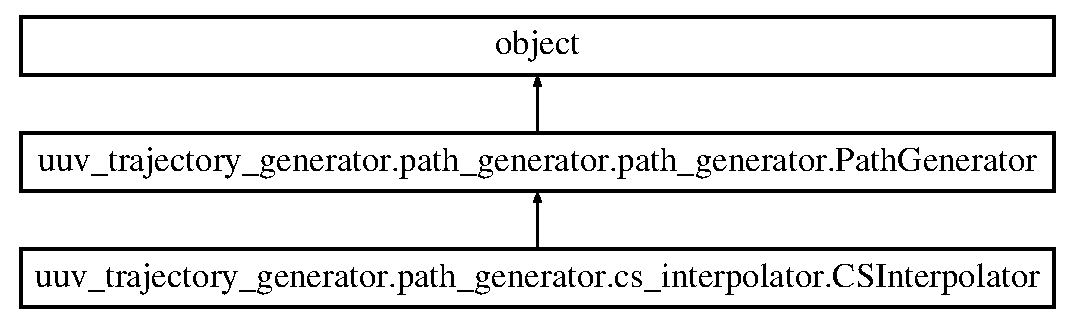
\includegraphics[height=3.000000cm]{classuuv__trajectory__generator_1_1path__generator_1_1cs__interpolator_1_1CSInterpolator}
\end{center}
\end{figure}
\subsection*{Public Member Functions}
\begin{DoxyCompactItemize}
\item 
\mbox{\Hypertarget{classuuv__trajectory__generator_1_1path__generator_1_1cs__interpolator_1_1CSInterpolator_ab5abe5006e2558313bc94fd667e260c9}\label{classuuv__trajectory__generator_1_1path__generator_1_1cs__interpolator_1_1CSInterpolator_ab5abe5006e2558313bc94fd667e260c9}} 
def {\bfseries \+\_\+\+\_\+init\+\_\+\+\_\+} (self)
\item 
\mbox{\Hypertarget{classuuv__trajectory__generator_1_1path__generator_1_1cs__interpolator_1_1CSInterpolator_a0362de5d6a59289ae15ce524bf50486e}\label{classuuv__trajectory__generator_1_1path__generator_1_1cs__interpolator_1_1CSInterpolator_a0362de5d6a59289ae15ce524bf50486e}} 
def {\bfseries init\+\_\+interpolator} (self)
\item 
def \hyperlink{classuuv__trajectory__generator_1_1path__generator_1_1cs__interpolator_1_1CSInterpolator_a5709f4bea7806927fd5d471bea615695}{set\+\_\+parameters} (self, params)
\item 
\mbox{\Hypertarget{classuuv__trajectory__generator_1_1path__generator_1_1cs__interpolator_1_1CSInterpolator_a001d024a504e763270a801db9369cc5f}\label{classuuv__trajectory__generator_1_1path__generator_1_1cs__interpolator_1_1CSInterpolator_a001d024a504e763270a801db9369cc5f}} 
def {\bfseries get\+\_\+samples} (self, max\+\_\+time, step=0.\+001)
\item 
\mbox{\Hypertarget{classuuv__trajectory__generator_1_1path__generator_1_1cs__interpolator_1_1CSInterpolator_a95dda4651417d524eb468a59a91608ff}\label{classuuv__trajectory__generator_1_1path__generator_1_1cs__interpolator_1_1CSInterpolator_a95dda4651417d524eb468a59a91608ff}} 
def {\bfseries generate\+\_\+pos} (self, s)
\item 
\mbox{\Hypertarget{classuuv__trajectory__generator_1_1path__generator_1_1cs__interpolator_1_1CSInterpolator_a0a80c3caad28d47c425270b3d45c3ece}\label{classuuv__trajectory__generator_1_1path__generator_1_1cs__interpolator_1_1CSInterpolator_a0a80c3caad28d47c425270b3d45c3ece}} 
def {\bfseries generate\+\_\+pnt} (self, s, t, args)
\item 
\mbox{\Hypertarget{classuuv__trajectory__generator_1_1path__generator_1_1cs__interpolator_1_1CSInterpolator_af7d91bfeabccf16d4d9095e9281abc74}\label{classuuv__trajectory__generator_1_1path__generator_1_1cs__interpolator_1_1CSInterpolator_af7d91bfeabccf16d4d9095e9281abc74}} 
def {\bfseries generate\+\_\+quat} (self, s)
\end{DoxyCompactItemize}
\subsection*{Static Public Attributes}
\begin{DoxyCompactItemize}
\item 
\mbox{\Hypertarget{classuuv__trajectory__generator_1_1path__generator_1_1cs__interpolator_1_1CSInterpolator_aaa519ab2cb687727d59a83dd4d5cf0b6}\label{classuuv__trajectory__generator_1_1path__generator_1_1cs__interpolator_1_1CSInterpolator_aaa519ab2cb687727d59a83dd4d5cf0b6}} 
string {\bfseries L\+A\+B\+EL} = \textquotesingle{}cubic\textquotesingle{}
\end{DoxyCompactItemize}
\subsection*{Additional Inherited Members}


\subsection{Detailed Description}
\begin{DoxyVerb}Interpolator that will generate cubic Bezier curve segments for a set of waypoints.
\end{DoxyVerb}
 

\subsection{Member Function Documentation}
\mbox{\Hypertarget{classuuv__trajectory__generator_1_1path__generator_1_1cs__interpolator_1_1CSInterpolator_a5709f4bea7806927fd5d471bea615695}\label{classuuv__trajectory__generator_1_1path__generator_1_1cs__interpolator_1_1CSInterpolator_a5709f4bea7806927fd5d471bea615695}} 
\index{uuv\+\_\+trajectory\+\_\+generator\+::path\+\_\+generator\+::cs\+\_\+interpolator\+::\+C\+S\+Interpolator@{uuv\+\_\+trajectory\+\_\+generator\+::path\+\_\+generator\+::cs\+\_\+interpolator\+::\+C\+S\+Interpolator}!set\+\_\+parameters@{set\+\_\+parameters}}
\index{set\+\_\+parameters@{set\+\_\+parameters}!uuv\+\_\+trajectory\+\_\+generator\+::path\+\_\+generator\+::cs\+\_\+interpolator\+::\+C\+S\+Interpolator@{uuv\+\_\+trajectory\+\_\+generator\+::path\+\_\+generator\+::cs\+\_\+interpolator\+::\+C\+S\+Interpolator}}
\subsubsection{\texorpdfstring{set\+\_\+parameters()}{set\_parameters()}}
{\footnotesize\ttfamily def uuv\+\_\+trajectory\+\_\+generator.\+path\+\_\+generator.\+cs\+\_\+interpolator.\+C\+S\+Interpolator.\+set\+\_\+parameters (\begin{DoxyParamCaption}\item[{}]{self,  }\item[{}]{params }\end{DoxyParamCaption})}

\begin{DoxyVerb}Not implemented for this interpolator.\end{DoxyVerb}
 

The documentation for this class was generated from the following file\+:\begin{DoxyCompactItemize}
\item 
control\+\_\+layer/uuv\+\_\+trajectory\+\_\+control/src/uuv\+\_\+trajectory\+\_\+generator/path\+\_\+generator/cs\+\_\+interpolator.\+py\end{DoxyCompactItemize}

\hypertarget{classmtdef_1_1DeprecatedMID}{}\doxysection{mtdef.\+Deprecated\+M\+ID Class Reference}
\label{classmtdef_1_1DeprecatedMID}\index{mtdef.DeprecatedMID@{mtdef.DeprecatedMID}}
\doxysubsection*{Static Public Attributes}
\begin{DoxyCompactItemize}
\item 
\mbox{\Hypertarget{classmtdef_1_1DeprecatedMID_a81f218692edadece8719f387f1b052c4}\label{classmtdef_1_1DeprecatedMID_a81f218692edadece8719f387f1b052c4}} 
int {\bfseries Init\+MT} = 0x02
\item 
\mbox{\Hypertarget{classmtdef_1_1DeprecatedMID_a04dbf68dfac7605603301e2543e979d6}\label{classmtdef_1_1DeprecatedMID_a04dbf68dfac7605603301e2543e979d6}} 
int {\bfseries Init\+M\+T\+Results} = 0x03
\item 
\mbox{\Hypertarget{classmtdef_1_1DeprecatedMID_a3f7ea58fbdaa107e85bb4346077f77c6}\label{classmtdef_1_1DeprecatedMID_a3f7ea58fbdaa107e85bb4346077f77c6}} 
int {\bfseries Req\+Data\+Length} = 0x0A
\item 
\mbox{\Hypertarget{classmtdef_1_1DeprecatedMID_a1f84b0b45629ab4fe1bea6254b8cc510}\label{classmtdef_1_1DeprecatedMID_a1f84b0b45629ab4fe1bea6254b8cc510}} 
int {\bfseries Data\+Length} = 0x0B
\item 
\mbox{\Hypertarget{classmtdef_1_1DeprecatedMID_a45521522a75d20365bab79113cc1c653}\label{classmtdef_1_1DeprecatedMID_a45521522a75d20365bab79113cc1c653}} 
int {\bfseries Req\+G\+P\+S\+Status} = 0x\+A6
\item 
\mbox{\Hypertarget{classmtdef_1_1DeprecatedMID_accd6581d6c16fc3bd3391f050454329a}\label{classmtdef_1_1DeprecatedMID_accd6581d6c16fc3bd3391f050454329a}} 
int {\bfseries G\+P\+S\+Status} = 0x\+A7
\item 
\mbox{\Hypertarget{classmtdef_1_1DeprecatedMID_a563024426a8966669e7f72739bfe04d7}\label{classmtdef_1_1DeprecatedMID_a563024426a8966669e7f72739bfe04d7}} 
int {\bfseries Set\+Sync\+In\+Settings} = 0x\+D6
\item 
\mbox{\Hypertarget{classmtdef_1_1DeprecatedMID_a19f16db2e567e12cf99e5379051e5cd5}\label{classmtdef_1_1DeprecatedMID_a19f16db2e567e12cf99e5379051e5cd5}} 
int {\bfseries Set\+Sync\+Out\+Settings} = 0x\+D8
\item 
\mbox{\Hypertarget{classmtdef_1_1DeprecatedMID_adbb3a554f4260576de132ce994b21419}\label{classmtdef_1_1DeprecatedMID_adbb3a554f4260576de132ce994b21419}} 
int {\bfseries Set\+Output\+Skip\+Factor} = 0x\+D4
\item 
\mbox{\Hypertarget{classmtdef_1_1DeprecatedMID_a5fd10d7480a4d49bef56fc0fc067513f}\label{classmtdef_1_1DeprecatedMID_a5fd10d7480a4d49bef56fc0fc067513f}} 
int {\bfseries Set\+Object\+Alignment} = 0x\+E0
\item 
\mbox{\Hypertarget{classmtdef_1_1DeprecatedMID_acea87b4dc1c35036d051716c8aa6b20f}\label{classmtdef_1_1DeprecatedMID_acea87b4dc1c35036d051716c8aa6b20f}} 
int {\bfseries Set\+Heading} = 0x82
\item 
\mbox{\Hypertarget{classmtdef_1_1DeprecatedMID_a64be0cab8c31a851b7d25f9a07352159}\label{classmtdef_1_1DeprecatedMID_a64be0cab8c31a851b7d25f9a07352159}} 
int {\bfseries Set\+Lever\+Arm\+G\+PS} = 0x68
\item 
\mbox{\Hypertarget{classmtdef_1_1DeprecatedMID_a6a5cedb0e51e2ea8673e3cf310ec7f7b}\label{classmtdef_1_1DeprecatedMID_a6a5cedb0e51e2ea8673e3cf310ec7f7b}} 
int {\bfseries Set\+Magnetic\+Declination} = 0x6A
\item 
\mbox{\Hypertarget{classmtdef_1_1DeprecatedMID_a98ba01a9bd9f16cc4941b1157696c72b}\label{classmtdef_1_1DeprecatedMID_a98ba01a9bd9f16cc4941b1157696c72b}} 
int {\bfseries Set\+Processing\+Flags} = 0x20
\end{DoxyCompactItemize}


\doxysubsection{Detailed Description}
\begin{DoxyVerb}Deprecated message Ids.\end{DoxyVerb}
 

The documentation for this class was generated from the following file\+:\begin{DoxyCompactItemize}
\item 
hardware\+\_\+layer/xsens\+\_\+driver/nodes/mtdef.\+py\end{DoxyCompactItemize}

\hypertarget{classimage__undistort_1_1Depth}{}\section{image\+\_\+undistort\+:\+:Depth Class Reference}
\label{classimage__undistort_1_1Depth}\index{image\+\_\+undistort\+::\+Depth@{image\+\_\+undistort\+::\+Depth}}
\subsection*{Public Member Functions}
\begin{DoxyCompactItemize}
\item 
\mbox{\Hypertarget{classimage__undistort_1_1Depth_a26bd724e80c82d7fe75c321b191b9cc0}\label{classimage__undistort_1_1Depth_a26bd724e80c82d7fe75c321b191b9cc0}} 
{\bfseries Depth} (const ros\+::\+Node\+Handle \&nh, const ros\+::\+Node\+Handle \&nh\+\_\+private)
\item 
\mbox{\Hypertarget{classimage__undistort_1_1Depth_a9a8f3bc5b26f64c3ebbd549cf25bb029}\label{classimage__undistort_1_1Depth_a9a8f3bc5b26f64c3ebbd549cf25bb029}} 
void {\bfseries cameras\+Callback} (const sensor\+\_\+msgs\+::\+Image\+Const\+Ptr \&first\+\_\+image\+\_\+msg\+\_\+in, const sensor\+\_\+msgs\+::\+Image\+Const\+Ptr \&second\+\_\+image\+\_\+msg\+\_\+in, const sensor\+\_\+msgs\+::\+Camera\+Info\+Const\+Ptr \&first\+\_\+camera\+\_\+info\+\_\+msg\+\_\+in, const sensor\+\_\+msgs\+::\+Camera\+Info\+Const\+Ptr \&second\+\_\+camera\+\_\+info\+\_\+msg\+\_\+in)
\end{DoxyCompactItemize}


The documentation for this class was generated from the following files\+:\begin{DoxyCompactItemize}
\item 
vision\+\_\+layer/image\+\_\+undistort/include/image\+\_\+undistort/depth.\+h\item 
vision\+\_\+layer/image\+\_\+undistort/src/depth.\+cpp\end{DoxyCompactItemize}

\hypertarget{classimage__undistort_1_1DepthNodelet}{}\doxysection{image\+\_\+undistort\+::Depth\+Nodelet Class Reference}
\label{classimage__undistort_1_1DepthNodelet}\index{image\_undistort::DepthNodelet@{image\_undistort::DepthNodelet}}
Inheritance diagram for image\+\_\+undistort\+::Depth\+Nodelet\+:\begin{figure}[H]
\begin{center}
\leavevmode
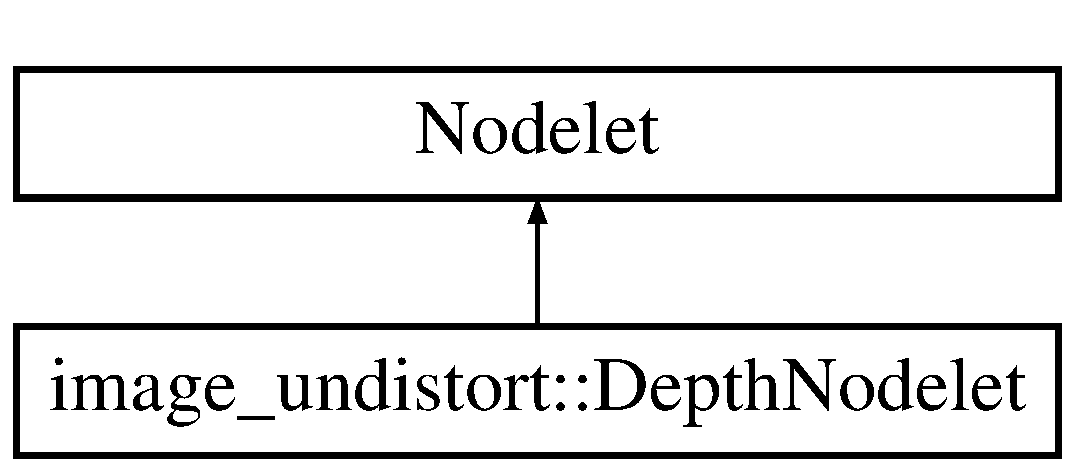
\includegraphics[height=2.000000cm]{classimage__undistort_1_1DepthNodelet}
\end{center}
\end{figure}


The documentation for this class was generated from the following file\+:\begin{DoxyCompactItemize}
\item 
vision\+\_\+layer/image\+\_\+undistort/src/nodelets/depth\+\_\+nodelet.\+cpp\end{DoxyCompactItemize}

\hypertarget{classmtdef_1_1DeviceState}{}\section{mtdef.\+Device\+State Class Reference}
\label{classmtdef_1_1DeviceState}\index{mtdef.\+Device\+State@{mtdef.\+Device\+State}}
\subsection*{Static Public Attributes}
\begin{DoxyCompactItemize}
\item 
\mbox{\Hypertarget{classmtdef_1_1DeviceState_a705b5ce4d7597d7a08be708c11003fc9}\label{classmtdef_1_1DeviceState_a705b5ce4d7597d7a08be708c11003fc9}} 
int {\bfseries Measurement} = 0
\item 
\mbox{\Hypertarget{classmtdef_1_1DeviceState_acf273cb71dcc1630fcce97d4f8850509}\label{classmtdef_1_1DeviceState_acf273cb71dcc1630fcce97d4f8850509}} 
int {\bfseries Config} = 1
\end{DoxyCompactItemize}


\subsection{Detailed Description}
\begin{DoxyVerb}State of the device\end{DoxyVerb}
 

The documentation for this class was generated from the following file\+:\begin{DoxyCompactItemize}
\item 
hardware\+\_\+layer/xsens\+\_\+driver/nodes/mtdef.\+py\end{DoxyCompactItemize}

\hypertarget{classdisturbance__manager_1_1DisturbanceManager}{}\section{disturbance\+\_\+manager.\+Disturbance\+Manager Class Reference}
\label{classdisturbance__manager_1_1DisturbanceManager}\index{disturbance\+\_\+manager.\+Disturbance\+Manager@{disturbance\+\_\+manager.\+Disturbance\+Manager}}
\subsection*{Public Member Functions}
\begin{DoxyCompactItemize}
\item 
\mbox{\Hypertarget{classdisturbance__manager_1_1DisturbanceManager_a0a5fb846386cbfd860c433826635ff7f}\label{classdisturbance__manager_1_1DisturbanceManager_a0a5fb846386cbfd860c433826635ff7f}} 
def {\bfseries \+\_\+\+\_\+init\+\_\+\+\_\+} (self)
\item 
\mbox{\Hypertarget{classdisturbance__manager_1_1DisturbanceManager_a15ae6c934d37756579f397bbed789927}\label{classdisturbance__manager_1_1DisturbanceManager_a15ae6c934d37756579f397bbed789927}} 
def {\bfseries set\+\_\+current} (self, velocity, horizontal\+\_\+angle, vertical\+\_\+angle)
\item 
\mbox{\Hypertarget{classdisturbance__manager_1_1DisturbanceManager_ae7e8a162ed42d8fa1835e6585cf27d4a}\label{classdisturbance__manager_1_1DisturbanceManager_ae7e8a162ed42d8fa1835e6585cf27d4a}} 
def {\bfseries set\+\_\+body\+\_\+wrench} (self, force, torque, duration, starting\+\_\+time)
\item 
\mbox{\Hypertarget{classdisturbance__manager_1_1DisturbanceManager_a3cfab35f2cfb1464c67baf6ac105c569}\label{classdisturbance__manager_1_1DisturbanceManager_a3cfab35f2cfb1464c67baf6ac105c569}} 
def {\bfseries set\+\_\+thruster\+\_\+state} (self, thruster\+\_\+id, is\+\_\+on)
\item 
\mbox{\Hypertarget{classdisturbance__manager_1_1DisturbanceManager_ad92f7bd8ecfb5b1e7db1bff8d040ae09}\label{classdisturbance__manager_1_1DisturbanceManager_ad92f7bd8ecfb5b1e7db1bff8d040ae09}} 
def {\bfseries set\+\_\+propeller\+\_\+efficiency} (self, thruster\+\_\+id, eff)
\item 
\mbox{\Hypertarget{classdisturbance__manager_1_1DisturbanceManager_a243a781bba7506bfc754c3890511a910}\label{classdisturbance__manager_1_1DisturbanceManager_a243a781bba7506bfc754c3890511a910}} 
def {\bfseries set\+\_\+thrust\+\_\+efficiency} (self, thruster\+\_\+id, eff)
\end{DoxyCompactItemize}


The documentation for this class was generated from the following file\+:\begin{DoxyCompactItemize}
\item 
control\+\_\+layer/uuv\+\_\+control\+\_\+utils/scripts/disturbance\+\_\+manager.\+py\end{DoxyCompactItemize}

\hypertarget{classuuv__control__interfaces_1_1dp__controller__base_1_1DPControllerBase}{}\section{uuv\+\_\+control\+\_\+interfaces.\+dp\+\_\+controller\+\_\+base.\+D\+P\+Controller\+Base Class Reference}
\label{classuuv__control__interfaces_1_1dp__controller__base_1_1DPControllerBase}\index{uuv\+\_\+control\+\_\+interfaces.\+dp\+\_\+controller\+\_\+base.\+D\+P\+Controller\+Base@{uuv\+\_\+control\+\_\+interfaces.\+dp\+\_\+controller\+\_\+base.\+D\+P\+Controller\+Base}}
Inheritance diagram for uuv\+\_\+control\+\_\+interfaces.\+dp\+\_\+controller\+\_\+base.\+D\+P\+Controller\+Base\+:\begin{figure}[H]
\begin{center}
\leavevmode
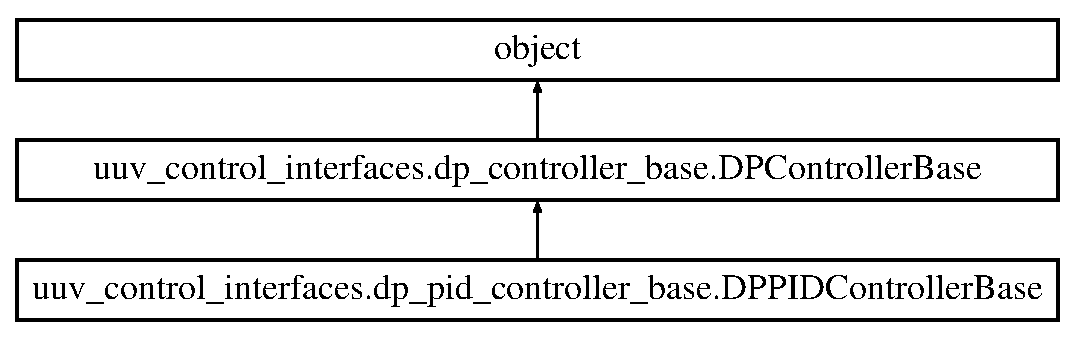
\includegraphics[height=3.000000cm]{classuuv__control__interfaces_1_1dp__controller__base_1_1DPControllerBase}
\end{center}
\end{figure}
\subsection*{Public Member Functions}
\begin{DoxyCompactItemize}
\item 
\mbox{\Hypertarget{classuuv__control__interfaces_1_1dp__controller__base_1_1DPControllerBase_a644ded1159688da231d1e76062e8c2ad}\label{classuuv__control__interfaces_1_1dp__controller__base_1_1DPControllerBase_a644ded1159688da231d1e76062e8c2ad}} 
def {\bfseries \+\_\+\+\_\+init\+\_\+\+\_\+} (self, is\+\_\+model\+\_\+based=False, list\+\_\+odometry\+\_\+callbacks=\mbox{[}$\,$\mbox{]}, planner\+\_\+full\+\_\+dof=False)
\item 
\mbox{\Hypertarget{classuuv__control__interfaces_1_1dp__controller__base_1_1DPControllerBase_afda5206a37fdd9ee99abdc11b64a32e6}\label{classuuv__control__interfaces_1_1dp__controller__base_1_1DPControllerBase_afda5206a37fdd9ee99abdc11b64a32e6}} 
def {\bfseries \+\_\+\+\_\+del\+\_\+\+\_\+} (self)
\item 
\mbox{\Hypertarget{classuuv__control__interfaces_1_1dp__controller__base_1_1DPControllerBase_a488b87b40157ffd1cd48d4103f734051}\label{classuuv__control__interfaces_1_1dp__controller__base_1_1DPControllerBase_a488b87b40157ffd1cd48d4103f734051}} 
def {\bfseries label} (self)
\item 
\mbox{\Hypertarget{classuuv__control__interfaces_1_1dp__controller__base_1_1DPControllerBase_a78abc01e4ed3b1d8339c7aa1b12caf1e}\label{classuuv__control__interfaces_1_1dp__controller__base_1_1DPControllerBase_a78abc01e4ed3b1d8339c7aa1b12caf1e}} 
def {\bfseries odom\+\_\+is\+\_\+init} (self)
\item 
\mbox{\Hypertarget{classuuv__control__interfaces_1_1dp__controller__base_1_1DPControllerBase_ac3b8069a7903de25a608ebe8a23cf304}\label{classuuv__control__interfaces_1_1dp__controller__base_1_1DPControllerBase_ac3b8069a7903de25a608ebe8a23cf304}} 
def {\bfseries error\+\_\+pos\+\_\+world} (self)
\item 
\mbox{\Hypertarget{classuuv__control__interfaces_1_1dp__controller__base_1_1DPControllerBase_afa7ca2e5aabf28567c733396aaefcc0a}\label{classuuv__control__interfaces_1_1dp__controller__base_1_1DPControllerBase_afa7ca2e5aabf28567c733396aaefcc0a}} 
def {\bfseries error\+\_\+orientation\+\_\+quat} (self)
\item 
def \hyperlink{classuuv__control__interfaces_1_1dp__controller__base_1_1DPControllerBase_a17876e9bc0c1dd2b0150e46b05cab56e}{error\+\_\+orientation\+\_\+rpy} (self)
\item 
def \hyperlink{classuuv__control__interfaces_1_1dp__controller__base_1_1DPControllerBase_a347226f1aa16d7464a666d4065083d36}{error\+\_\+pose\+\_\+euler} (self)
\item 
\mbox{\Hypertarget{classuuv__control__interfaces_1_1dp__controller__base_1_1DPControllerBase_aeecc142f3eb8d3ac49e7c7a9417debfa}\label{classuuv__control__interfaces_1_1dp__controller__base_1_1DPControllerBase_aeecc142f3eb8d3ac49e7c7a9417debfa}} 
def {\bfseries error\+\_\+vel\+\_\+world} (self)
\item 
\mbox{\Hypertarget{classuuv__control__interfaces_1_1dp__controller__base_1_1DPControllerBase_a5c9cd62adf1d2c2c2fa05fe751dcf5d7}\label{classuuv__control__interfaces_1_1dp__controller__base_1_1DPControllerBase_a5c9cd62adf1d2c2c2fa05fe751dcf5d7}} 
def {\bfseries \+\_\+\+\_\+str\+\_\+\+\_\+} (self)
\item 
\mbox{\Hypertarget{classuuv__control__interfaces_1_1dp__controller__base_1_1DPControllerBase_a644a7e9c1d7c97fb7e9ab7c1fbfb9d18}\label{classuuv__control__interfaces_1_1dp__controller__base_1_1DPControllerBase_a644a7e9c1d7c97fb7e9ab7c1fbfb9d18}} 
def {\bfseries reset\+\_\+controller\+\_\+callback} (self, request)
\item 
\mbox{\Hypertarget{classuuv__control__interfaces_1_1dp__controller__base_1_1DPControllerBase_a3a8deb68f36e9deb74551b27a7f08e37}\label{classuuv__control__interfaces_1_1dp__controller__base_1_1DPControllerBase_a3a8deb68f36e9deb74551b27a7f08e37}} 
def {\bfseries update\+\_\+controller} (self)
\item 
\mbox{\Hypertarget{classuuv__control__interfaces_1_1dp__controller__base_1_1DPControllerBase_a7fbba860e696aab5f3c129a0459042cc}\label{classuuv__control__interfaces_1_1dp__controller__base_1_1DPControllerBase_a7fbba860e696aab5f3c129a0459042cc}} 
def {\bfseries update\+\_\+errors} (self)
\item 
\mbox{\Hypertarget{classuuv__control__interfaces_1_1dp__controller__base_1_1DPControllerBase_acf544643f1372f44521feb9c7e2f9e92}\label{classuuv__control__interfaces_1_1dp__controller__base_1_1DPControllerBase_acf544643f1372f44521feb9c7e2f9e92}} 
def {\bfseries publish\+\_\+control\+\_\+wrench} (self, force)
\item 
\mbox{\Hypertarget{classuuv__control__interfaces_1_1dp__controller__base_1_1DPControllerBase_a1214dc960d8bda0bafb5540dc3db56a1}\label{classuuv__control__interfaces_1_1dp__controller__base_1_1DPControllerBase_a1214dc960d8bda0bafb5540dc3db56a1}} 
def {\bfseries publish\+\_\+auv\+\_\+command} (self, surge\+\_\+speed, wrench)
\end{DoxyCompactItemize}
\subsection*{Static Public Member Functions}
\begin{DoxyCompactItemize}
\item 
def \hyperlink{classuuv__control__interfaces_1_1dp__controller__base_1_1DPControllerBase_aec486afa9f41a809450cf8c20d899dcc}{get\+\_\+controller} (\hyperlink{classname}{name}, args)
\item 
def \hyperlink{classuuv__control__interfaces_1_1dp__controller__base_1_1DPControllerBase_a7ce49bfa0863fb7c1f0fd2a438d53133}{get\+\_\+list\+\_\+of\+\_\+controllers} ()
\end{DoxyCompactItemize}
\subsection*{Public Attributes}
\begin{DoxyCompactItemize}
\item 
\mbox{\Hypertarget{classuuv__control__interfaces_1_1dp__controller__base_1_1DPControllerBase_ab900a68aa3ff5cfeaa32f96e6684bd6f}\label{classuuv__control__interfaces_1_1dp__controller__base_1_1DPControllerBase_ab900a68aa3ff5cfeaa32f96e6684bd6f}} 
{\bfseries thrusters\+\_\+only}
\item 
\mbox{\Hypertarget{classuuv__control__interfaces_1_1dp__controller__base_1_1DPControllerBase_a729d24e3222dab5e4c16a2e7b07ee34f}\label{classuuv__control__interfaces_1_1dp__controller__base_1_1DPControllerBase_a729d24e3222dab5e4c16a2e7b07ee34f}} 
{\bfseries use\+\_\+auv\+\_\+control\+\_\+allocator}
\end{DoxyCompactItemize}


\subsection{Detailed Description}
\begin{DoxyVerb}General abstract class for DP controllers for underwater vehicles.
This is an abstract class, must be inherited by a controller module that
overrides the update_controller method. If the controller is set to be
model based (is_model_based=True), than the vehicle parameters are going
to be read from the ROS parameter server.
\end{DoxyVerb}
 

\subsection{Member Function Documentation}
\mbox{\Hypertarget{classuuv__control__interfaces_1_1dp__controller__base_1_1DPControllerBase_a17876e9bc0c1dd2b0150e46b05cab56e}\label{classuuv__control__interfaces_1_1dp__controller__base_1_1DPControllerBase_a17876e9bc0c1dd2b0150e46b05cab56e}} 
\index{uuv\+\_\+control\+\_\+interfaces\+::dp\+\_\+controller\+\_\+base\+::\+D\+P\+Controller\+Base@{uuv\+\_\+control\+\_\+interfaces\+::dp\+\_\+controller\+\_\+base\+::\+D\+P\+Controller\+Base}!error\+\_\+orientation\+\_\+rpy@{error\+\_\+orientation\+\_\+rpy}}
\index{error\+\_\+orientation\+\_\+rpy@{error\+\_\+orientation\+\_\+rpy}!uuv\+\_\+control\+\_\+interfaces\+::dp\+\_\+controller\+\_\+base\+::\+D\+P\+Controller\+Base@{uuv\+\_\+control\+\_\+interfaces\+::dp\+\_\+controller\+\_\+base\+::\+D\+P\+Controller\+Base}}
\subsubsection{\texorpdfstring{error\+\_\+orientation\+\_\+rpy()}{error\_orientation\_rpy()}}
{\footnotesize\ttfamily def uuv\+\_\+control\+\_\+interfaces.\+dp\+\_\+controller\+\_\+base.\+D\+P\+Controller\+Base.\+error\+\_\+orientation\+\_\+rpy (\begin{DoxyParamCaption}\item[{}]{self }\end{DoxyParamCaption})}

\begin{DoxyVerb}Return orientation error in Euler angles.\end{DoxyVerb}
 \mbox{\Hypertarget{classuuv__control__interfaces_1_1dp__controller__base_1_1DPControllerBase_a347226f1aa16d7464a666d4065083d36}\label{classuuv__control__interfaces_1_1dp__controller__base_1_1DPControllerBase_a347226f1aa16d7464a666d4065083d36}} 
\index{uuv\+\_\+control\+\_\+interfaces\+::dp\+\_\+controller\+\_\+base\+::\+D\+P\+Controller\+Base@{uuv\+\_\+control\+\_\+interfaces\+::dp\+\_\+controller\+\_\+base\+::\+D\+P\+Controller\+Base}!error\+\_\+pose\+\_\+euler@{error\+\_\+pose\+\_\+euler}}
\index{error\+\_\+pose\+\_\+euler@{error\+\_\+pose\+\_\+euler}!uuv\+\_\+control\+\_\+interfaces\+::dp\+\_\+controller\+\_\+base\+::\+D\+P\+Controller\+Base@{uuv\+\_\+control\+\_\+interfaces\+::dp\+\_\+controller\+\_\+base\+::\+D\+P\+Controller\+Base}}
\subsubsection{\texorpdfstring{error\+\_\+pose\+\_\+euler()}{error\_pose\_euler()}}
{\footnotesize\ttfamily def uuv\+\_\+control\+\_\+interfaces.\+dp\+\_\+controller\+\_\+base.\+D\+P\+Controller\+Base.\+error\+\_\+pose\+\_\+euler (\begin{DoxyParamCaption}\item[{}]{self }\end{DoxyParamCaption})}

\begin{DoxyVerb}Pose error with orientation represented in Euler angles.\end{DoxyVerb}
 \mbox{\Hypertarget{classuuv__control__interfaces_1_1dp__controller__base_1_1DPControllerBase_aec486afa9f41a809450cf8c20d899dcc}\label{classuuv__control__interfaces_1_1dp__controller__base_1_1DPControllerBase_aec486afa9f41a809450cf8c20d899dcc}} 
\index{uuv\+\_\+control\+\_\+interfaces\+::dp\+\_\+controller\+\_\+base\+::\+D\+P\+Controller\+Base@{uuv\+\_\+control\+\_\+interfaces\+::dp\+\_\+controller\+\_\+base\+::\+D\+P\+Controller\+Base}!get\+\_\+controller@{get\+\_\+controller}}
\index{get\+\_\+controller@{get\+\_\+controller}!uuv\+\_\+control\+\_\+interfaces\+::dp\+\_\+controller\+\_\+base\+::\+D\+P\+Controller\+Base@{uuv\+\_\+control\+\_\+interfaces\+::dp\+\_\+controller\+\_\+base\+::\+D\+P\+Controller\+Base}}
\subsubsection{\texorpdfstring{get\+\_\+controller()}{get\_controller()}}
{\footnotesize\ttfamily def uuv\+\_\+control\+\_\+interfaces.\+dp\+\_\+controller\+\_\+base.\+D\+P\+Controller\+Base.\+get\+\_\+controller (\begin{DoxyParamCaption}\item[{}]{name,  }\item[{}]{args }\end{DoxyParamCaption})\hspace{0.3cm}{\ttfamily [static]}}

\begin{DoxyVerb}Create instance of a specific DP controller.\end{DoxyVerb}
 \mbox{\Hypertarget{classuuv__control__interfaces_1_1dp__controller__base_1_1DPControllerBase_a7ce49bfa0863fb7c1f0fd2a438d53133}\label{classuuv__control__interfaces_1_1dp__controller__base_1_1DPControllerBase_a7ce49bfa0863fb7c1f0fd2a438d53133}} 
\index{uuv\+\_\+control\+\_\+interfaces\+::dp\+\_\+controller\+\_\+base\+::\+D\+P\+Controller\+Base@{uuv\+\_\+control\+\_\+interfaces\+::dp\+\_\+controller\+\_\+base\+::\+D\+P\+Controller\+Base}!get\+\_\+list\+\_\+of\+\_\+controllers@{get\+\_\+list\+\_\+of\+\_\+controllers}}
\index{get\+\_\+list\+\_\+of\+\_\+controllers@{get\+\_\+list\+\_\+of\+\_\+controllers}!uuv\+\_\+control\+\_\+interfaces\+::dp\+\_\+controller\+\_\+base\+::\+D\+P\+Controller\+Base@{uuv\+\_\+control\+\_\+interfaces\+::dp\+\_\+controller\+\_\+base\+::\+D\+P\+Controller\+Base}}
\subsubsection{\texorpdfstring{get\+\_\+list\+\_\+of\+\_\+controllers()}{get\_list\_of\_controllers()}}
{\footnotesize\ttfamily def uuv\+\_\+control\+\_\+interfaces.\+dp\+\_\+controller\+\_\+base.\+D\+P\+Controller\+Base.\+get\+\_\+list\+\_\+of\+\_\+controllers (\begin{DoxyParamCaption}{ }\end{DoxyParamCaption})\hspace{0.3cm}{\ttfamily [static]}}

\begin{DoxyVerb}Return list of DP controllers using this interface.\end{DoxyVerb}
 

The documentation for this class was generated from the following file\+:\begin{DoxyCompactItemize}
\item 
control\+\_\+layer/uuv\+\_\+trajectory\+\_\+control/src/uuv\+\_\+control\+\_\+interfaces/dp\+\_\+controller\+\_\+base.\+py\end{DoxyCompactItemize}

\hypertarget{classuuv__control__interfaces_1_1dp__controller__local__planner_1_1DPControllerLocalPlanner}{}\doxysection{uuv\+\_\+control\+\_\+interfaces.\+dp\+\_\+controller\+\_\+local\+\_\+planner.\+D\+P\+Controller\+Local\+Planner Class Reference}
\label{classuuv__control__interfaces_1_1dp__controller__local__planner_1_1DPControllerLocalPlanner}\index{uuv\_control\_interfaces.dp\_controller\_local\_planner.DPControllerLocalPlanner@{uuv\_control\_interfaces.dp\_controller\_local\_planner.DPControllerLocalPlanner}}
Inheritance diagram for uuv\+\_\+control\+\_\+interfaces.\+dp\+\_\+controller\+\_\+local\+\_\+planner.\+D\+P\+Controller\+Local\+Planner\+:\begin{figure}[H]
\begin{center}
\leavevmode
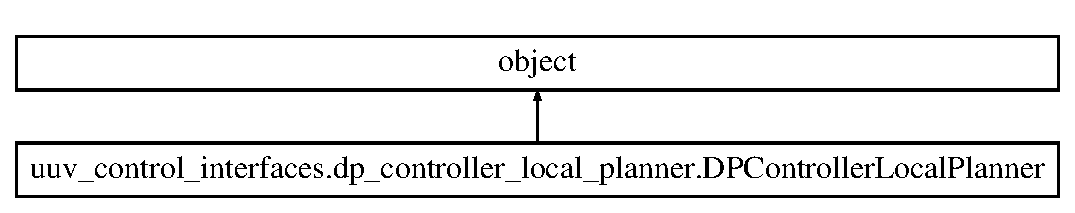
\includegraphics[height=2.000000cm]{classuuv__control__interfaces_1_1dp__controller__local__planner_1_1DPControllerLocalPlanner}
\end{center}
\end{figure}
\doxysubsection*{Public Member Functions}
\begin{DoxyCompactItemize}
\item 
\mbox{\Hypertarget{classuuv__control__interfaces_1_1dp__controller__local__planner_1_1DPControllerLocalPlanner_a9f9cf285950251ce33098d5ed2a2c75a}\label{classuuv__control__interfaces_1_1dp__controller__local__planner_1_1DPControllerLocalPlanner_a9f9cf285950251ce33098d5ed2a2c75a}} 
def {\bfseries \+\_\+\+\_\+init\+\_\+\+\_\+} (self, full\+\_\+dof=False, stamped\+\_\+pose\+\_\+only=False, thrusters\+\_\+only=True)
\item 
def \mbox{\hyperlink{classuuv__control__interfaces_1_1dp__controller__local__planner_1_1DPControllerLocalPlanner_a1e359e0c4268f8587f0a2cab1d545a74}{\+\_\+\+\_\+del\+\_\+\+\_\+}} (self)
\item 
\mbox{\Hypertarget{classuuv__control__interfaces_1_1dp__controller__local__planner_1_1DPControllerLocalPlanner_a19a70bed9ae0001434ff4cfce4963ab3}\label{classuuv__control__interfaces_1_1dp__controller__local__planner_1_1DPControllerLocalPlanner_a19a70bed9ae0001434ff4cfce4963ab3}} 
def {\bfseries is\+\_\+station\+\_\+keeping\+\_\+on} (self)
\item 
\mbox{\Hypertarget{classuuv__control__interfaces_1_1dp__controller__local__planner_1_1DPControllerLocalPlanner_a00dcadecc3c28660de8e41ac0f06f4db}\label{classuuv__control__interfaces_1_1dp__controller__local__planner_1_1DPControllerLocalPlanner_a00dcadecc3c28660de8e41ac0f06f4db}} 
def {\bfseries set\+\_\+stall\+\_\+vehicle} (self, is\+\_\+on=True)
\item 
\mbox{\Hypertarget{classuuv__control__interfaces_1_1dp__controller__local__planner_1_1DPControllerLocalPlanner_ac0cb56e9cb16f4249a222bc2d93c5a57}\label{classuuv__control__interfaces_1_1dp__controller__local__planner_1_1DPControllerLocalPlanner_ac0cb56e9cb16f4249a222bc2d93c5a57}} 
def {\bfseries is\+\_\+automatic\+\_\+on} (self)
\item 
def \mbox{\hyperlink{classuuv__control__interfaces_1_1dp__controller__local__planner_1_1DPControllerLocalPlanner_a8e6d4a2721e5d6eda14386c8cfe3e6c4}{set\+\_\+station\+\_\+keeping}} (self, is\+\_\+on=True)
\item 
def \mbox{\hyperlink{classuuv__control__interfaces_1_1dp__controller__local__planner_1_1DPControllerLocalPlanner_acbe4ccf881650464969425b43d76a633}{set\+\_\+automatic\+\_\+mode}} (self, is\+\_\+on=True)
\item 
def \mbox{\hyperlink{classuuv__control__interfaces_1_1dp__controller__local__planner_1_1DPControllerLocalPlanner_a919c977ffbee96552fdc3ac97776e994}{set\+\_\+trajectory\+\_\+running}} (self, is\+\_\+on=True)
\item 
def \mbox{\hyperlink{classuuv__control__interfaces_1_1dp__controller__local__planner_1_1DPControllerLocalPlanner_a1ae7c5245233d9f4b969a0ec9be1116a}{has\+\_\+started}} (self)
\item 
\mbox{\Hypertarget{classuuv__control__interfaces_1_1dp__controller__local__planner_1_1DPControllerLocalPlanner_af2d4b9aaf785ad8cec28ab624b476ba3}\label{classuuv__control__interfaces_1_1dp__controller__local__planner_1_1DPControllerLocalPlanner_af2d4b9aaf785ad8cec28ab624b476ba3}} 
def {\bfseries calc\+\_\+dist} (self)
\item 
\mbox{\Hypertarget{classuuv__control__interfaces_1_1dp__controller__local__planner_1_1DPControllerLocalPlanner_a0904dcac5e2f14c41cdb929701bb22cf}\label{classuuv__control__interfaces_1_1dp__controller__local__planner_1_1DPControllerLocalPlanner_a0904dcac5e2f14c41cdb929701bb22cf}} 
def {\bfseries has\+\_\+finished} (self)
\item 
\mbox{\Hypertarget{classuuv__control__interfaces_1_1dp__controller__local__planner_1_1DPControllerLocalPlanner_a701c60da037da4fccb389f994f75e546}\label{classuuv__control__interfaces_1_1dp__controller__local__planner_1_1DPControllerLocalPlanner_a701c60da037da4fccb389f994f75e546}} 
def {\bfseries update\+\_\+vehicle\+\_\+pose} (self, pos, quat)
\item 
\mbox{\Hypertarget{classuuv__control__interfaces_1_1dp__controller__local__planner_1_1DPControllerLocalPlanner_a569c7f6357d325265309ac753f5c32e4}\label{classuuv__control__interfaces_1_1dp__controller__local__planner_1_1DPControllerLocalPlanner_a569c7f6357d325265309ac753f5c32e4}} 
def {\bfseries get\+\_\+vehicle\+\_\+rot} (self)
\item 
\mbox{\Hypertarget{classuuv__control__interfaces_1_1dp__controller__local__planner_1_1DPControllerLocalPlanner_aea5fe461a5293f0729e1948d2402a122}\label{classuuv__control__interfaces_1_1dp__controller__local__planner_1_1DPControllerLocalPlanner_aea5fe461a5293f0729e1948d2402a122}} 
def {\bfseries start\+\_\+station\+\_\+keeping} (self)
\item 
def \mbox{\hyperlink{classuuv__control__interfaces_1_1dp__controller__local__planner_1_1DPControllerLocalPlanner_a6bd23a0405943515adbadeed5b594024}{hold\+\_\+vehicle}} (self, request)
\item 
\mbox{\Hypertarget{classuuv__control__interfaces_1_1dp__controller__local__planner_1_1DPControllerLocalPlanner_ad5e4906bd745b426b1065ae846a9f441}\label{classuuv__control__interfaces_1_1dp__controller__local__planner_1_1DPControllerLocalPlanner_ad5e4906bd745b426b1065ae846a9f441}} 
def {\bfseries cancel\+\_\+request} (self, request)
\item 
\mbox{\Hypertarget{classuuv__control__interfaces_1_1dp__controller__local__planner_1_1DPControllerLocalPlanner_ae5e2c789554fb2722e981861e7c0944c}\label{classuuv__control__interfaces_1_1dp__controller__local__planner_1_1DPControllerLocalPlanner_ae5e2c789554fb2722e981861e7c0944c}} 
def {\bfseries bottom\+\_\+manoeuvre} (self, request)
\item 
\mbox{\Hypertarget{classuuv__control__interfaces_1_1dp__controller__local__planner_1_1DPControllerLocalPlanner_a31c617bee95786d64c1a28dc05569d9e}\label{classuuv__control__interfaces_1_1dp__controller__local__planner_1_1DPControllerLocalPlanner_a31c617bee95786d64c1a28dc05569d9e}} 
def {\bfseries front\+\_\+manoeuvre} (self, request)
\item 
def \mbox{\hyperlink{classuuv__control__interfaces_1_1dp__controller__local__planner_1_1DPControllerLocalPlanner_a6bd6967b8b081c393cca5e71f1b3d022}{go\+\_\+to\+\_\+pose}} (self, request)
\item 
\mbox{\Hypertarget{classuuv__control__interfaces_1_1dp__controller__local__planner_1_1DPControllerLocalPlanner_a0263115133417eedf16c5c205ba095f1}\label{classuuv__control__interfaces_1_1dp__controller__local__planner_1_1DPControllerLocalPlanner_a0263115133417eedf16c5c205ba095f1}} 
def {\bfseries has\+\_\+reached\+\_\+pose} (self)
\item 
\mbox{\Hypertarget{classuuv__control__interfaces_1_1dp__controller__local__planner_1_1DPControllerLocalPlanner_acb2463514d0eb3e11b151b9449d402e0}\label{classuuv__control__interfaces_1_1dp__controller__local__planner_1_1DPControllerLocalPlanner_acb2463514d0eb3e11b151b9449d402e0}} 
def {\bfseries is\+\_\+trajectory\+\_\+complete} (self, request)
\item 
def \mbox{\hyperlink{classuuv__control__interfaces_1_1dp__controller__local__planner_1_1DPControllerLocalPlanner_a46a25930563b91150b7c8282b028d7fa}{start\+\_\+waypoint\+\_\+list}} (self, request)
\item 
\mbox{\Hypertarget{classuuv__control__interfaces_1_1dp__controller__local__planner_1_1DPControllerLocalPlanner_a6d96af27a6aebf3865209d5dce62e4ad}\label{classuuv__control__interfaces_1_1dp__controller__local__planner_1_1DPControllerLocalPlanner_a6d96af27a6aebf3865209d5dce62e4ad}} 
def {\bfseries start\+\_\+circle} (self, request)
\item 
\mbox{\Hypertarget{classuuv__control__interfaces_1_1dp__controller__local__planner_1_1DPControllerLocalPlanner_a85376a66e492305f37146201d3337fdc}\label{classuuv__control__interfaces_1_1dp__controller__local__planner_1_1DPControllerLocalPlanner_a85376a66e492305f37146201d3337fdc}} 
def {\bfseries start\+\_\+helix} (self, request)
\item 
\mbox{\Hypertarget{classuuv__control__interfaces_1_1dp__controller__local__planner_1_1DPControllerLocalPlanner_a2db746fdcd728ce45b6b6554bd630735}\label{classuuv__control__interfaces_1_1dp__controller__local__planner_1_1DPControllerLocalPlanner_a2db746fdcd728ce45b6b6554bd630735}} 
def {\bfseries init\+\_\+waypoints\+\_\+from\+\_\+file} (self, request)
\item 
\mbox{\Hypertarget{classuuv__control__interfaces_1_1dp__controller__local__planner_1_1DPControllerLocalPlanner_a8139529ba72a5870c7a80ab5b1e476a7}\label{classuuv__control__interfaces_1_1dp__controller__local__planner_1_1DPControllerLocalPlanner_a8139529ba72a5870c7a80ab5b1e476a7}} 
def {\bfseries go\+\_\+to} (self, request)
\item 
def \mbox{\hyperlink{classuuv__control__interfaces_1_1dp__controller__local__planner_1_1DPControllerLocalPlanner_a837e655206c606eb9441e5a8053556a0}{go\+\_\+to\+\_\+incremental}} (self, request)
\item 
\mbox{\Hypertarget{classuuv__control__interfaces_1_1dp__controller__local__planner_1_1DPControllerLocalPlanner_a27a33f37e95c3c9f5b02da313c7cafdc}\label{classuuv__control__interfaces_1_1dp__controller__local__planner_1_1DPControllerLocalPlanner_a27a33f37e95c3c9f5b02da313c7cafdc}} 
def {\bfseries generate\+\_\+reference} (self, t)
\item 
\mbox{\Hypertarget{classuuv__control__interfaces_1_1dp__controller__local__planner_1_1DPControllerLocalPlanner_af6bca3f06940f796a23520f214f0d11a}\label{classuuv__control__interfaces_1_1dp__controller__local__planner_1_1DPControllerLocalPlanner_af6bca3f06940f796a23520f214f0d11a}} 
def {\bfseries get\+\_\+idle\+\_\+circle\+\_\+path} (self, n\+\_\+points, radius=30)
\item 
def \mbox{\hyperlink{classuuv__control__interfaces_1_1dp__controller__local__planner_1_1DPControllerLocalPlanner_a83e315388b12f1119fcb3363a6ce6cf2}{interpolate}} (self, t)
\end{DoxyCompactItemize}
\doxysubsection*{Public Attributes}
\begin{DoxyCompactItemize}
\item 
\mbox{\Hypertarget{classuuv__control__interfaces_1_1dp__controller__local__planner_1_1DPControllerLocalPlanner_a5a6cc0e2d5d1c42066b112e0f025c61c}\label{classuuv__control__interfaces_1_1dp__controller__local__planner_1_1DPControllerLocalPlanner_a5a6cc0e2d5d1c42066b112e0f025c61c}} 
{\bfseries inertial\+\_\+frame\+\_\+id}
\item 
\mbox{\Hypertarget{classuuv__control__interfaces_1_1dp__controller__local__planner_1_1DPControllerLocalPlanner_ad3a8c5ab28046c40d370ed1d2832946b}\label{classuuv__control__interfaces_1_1dp__controller__local__planner_1_1DPControllerLocalPlanner_ad3a8c5ab28046c40d370ed1d2832946b}} 
{\bfseries transform\+\_\+ned\+\_\+to\+\_\+enu}
\item 
\mbox{\Hypertarget{classuuv__control__interfaces_1_1dp__controller__local__planner_1_1DPControllerLocalPlanner_a5b97450dceb16453b500e1f6a550c35a}\label{classuuv__control__interfaces_1_1dp__controller__local__planner_1_1DPControllerLocalPlanner_a5b97450dceb16453b500e1f6a550c35a}} 
{\bfseries q\+\_\+ned\+\_\+to\+\_\+enu}
\item 
\mbox{\Hypertarget{classuuv__control__interfaces_1_1dp__controller__local__planner_1_1DPControllerLocalPlanner_a69cf51ff8072fafa937f4ffe3467a5a4}\label{classuuv__control__interfaces_1_1dp__controller__local__planner_1_1DPControllerLocalPlanner_a69cf51ff8072fafa937f4ffe3467a5a4}} 
{\bfseries init\+\_\+odom\+\_\+event}
\end{DoxyCompactItemize}


\doxysubsection{Detailed Description}
\begin{DoxyVerb}Local planner for the dynamic positioning controllers to interpolate
trajectories and generate trajectories from interpolated waypoint paths.
\end{DoxyVerb}
 

\doxysubsection{Constructor \& Destructor Documentation}
\mbox{\Hypertarget{classuuv__control__interfaces_1_1dp__controller__local__planner_1_1DPControllerLocalPlanner_a1e359e0c4268f8587f0a2cab1d545a74}\label{classuuv__control__interfaces_1_1dp__controller__local__planner_1_1DPControllerLocalPlanner_a1e359e0c4268f8587f0a2cab1d545a74}} 
\index{uuv\_control\_interfaces.dp\_controller\_local\_planner.DPControllerLocalPlanner@{uuv\_control\_interfaces.dp\_controller\_local\_planner.DPControllerLocalPlanner}!\_\_del\_\_@{\_\_del\_\_}}
\index{\_\_del\_\_@{\_\_del\_\_}!uuv\_control\_interfaces.dp\_controller\_local\_planner.DPControllerLocalPlanner@{uuv\_control\_interfaces.dp\_controller\_local\_planner.DPControllerLocalPlanner}}
\doxysubsubsection{\texorpdfstring{\_\_del\_\_()}{\_\_del\_\_()}}
{\footnotesize\ttfamily def uuv\+\_\+control\+\_\+interfaces.\+dp\+\_\+controller\+\_\+local\+\_\+planner.\+D\+P\+Controller\+Local\+Planner.\+\_\+\+\_\+del\+\_\+\+\_\+ (\begin{DoxyParamCaption}\item[{}]{self }\end{DoxyParamCaption})}

\begin{DoxyVerb}Remove logging message handlers\end{DoxyVerb}
 

\doxysubsection{Member Function Documentation}
\mbox{\Hypertarget{classuuv__control__interfaces_1_1dp__controller__local__planner_1_1DPControllerLocalPlanner_a837e655206c606eb9441e5a8053556a0}\label{classuuv__control__interfaces_1_1dp__controller__local__planner_1_1DPControllerLocalPlanner_a837e655206c606eb9441e5a8053556a0}} 
\index{uuv\_control\_interfaces.dp\_controller\_local\_planner.DPControllerLocalPlanner@{uuv\_control\_interfaces.dp\_controller\_local\_planner.DPControllerLocalPlanner}!go\_to\_incremental@{go\_to\_incremental}}
\index{go\_to\_incremental@{go\_to\_incremental}!uuv\_control\_interfaces.dp\_controller\_local\_planner.DPControllerLocalPlanner@{uuv\_control\_interfaces.dp\_controller\_local\_planner.DPControllerLocalPlanner}}
\doxysubsubsection{\texorpdfstring{go\_to\_incremental()}{go\_to\_incremental()}}
{\footnotesize\ttfamily def uuv\+\_\+control\+\_\+interfaces.\+dp\+\_\+controller\+\_\+local\+\_\+planner.\+D\+P\+Controller\+Local\+Planner.\+go\+\_\+to\+\_\+incremental (\begin{DoxyParamCaption}\item[{}]{self,  }\item[{}]{request }\end{DoxyParamCaption})}

\begin{DoxyVerb}Service callback to set the command to the vehicle to move to a
relative position in the world.
\end{DoxyVerb}
 \mbox{\Hypertarget{classuuv__control__interfaces_1_1dp__controller__local__planner_1_1DPControllerLocalPlanner_a6bd6967b8b081c393cca5e71f1b3d022}\label{classuuv__control__interfaces_1_1dp__controller__local__planner_1_1DPControllerLocalPlanner_a6bd6967b8b081c393cca5e71f1b3d022}} 
\index{uuv\_control\_interfaces.dp\_controller\_local\_planner.DPControllerLocalPlanner@{uuv\_control\_interfaces.dp\_controller\_local\_planner.DPControllerLocalPlanner}!go\_to\_pose@{go\_to\_pose}}
\index{go\_to\_pose@{go\_to\_pose}!uuv\_control\_interfaces.dp\_controller\_local\_planner.DPControllerLocalPlanner@{uuv\_control\_interfaces.dp\_controller\_local\_planner.DPControllerLocalPlanner}}
\doxysubsubsection{\texorpdfstring{go\_to\_pose()}{go\_to\_pose()}}
{\footnotesize\ttfamily def uuv\+\_\+control\+\_\+interfaces.\+dp\+\_\+controller\+\_\+local\+\_\+planner.\+D\+P\+Controller\+Local\+Planner.\+go\+\_\+to\+\_\+pose (\begin{DoxyParamCaption}\item[{}]{self,  }\item[{}]{request }\end{DoxyParamCaption})}

\begin{DoxyVerb}Service callback function to achieve a certain pose
\end{DoxyVerb}
 \mbox{\Hypertarget{classuuv__control__interfaces_1_1dp__controller__local__planner_1_1DPControllerLocalPlanner_a1ae7c5245233d9f4b969a0ec9be1116a}\label{classuuv__control__interfaces_1_1dp__controller__local__planner_1_1DPControllerLocalPlanner_a1ae7c5245233d9f4b969a0ec9be1116a}} 
\index{uuv\_control\_interfaces.dp\_controller\_local\_planner.DPControllerLocalPlanner@{uuv\_control\_interfaces.dp\_controller\_local\_planner.DPControllerLocalPlanner}!has\_started@{has\_started}}
\index{has\_started@{has\_started}!uuv\_control\_interfaces.dp\_controller\_local\_planner.DPControllerLocalPlanner@{uuv\_control\_interfaces.dp\_controller\_local\_planner.DPControllerLocalPlanner}}
\doxysubsubsection{\texorpdfstring{has\_started()}{has\_started()}}
{\footnotesize\ttfamily def uuv\+\_\+control\+\_\+interfaces.\+dp\+\_\+controller\+\_\+local\+\_\+planner.\+D\+P\+Controller\+Local\+Planner.\+has\+\_\+started (\begin{DoxyParamCaption}\item[{}]{self }\end{DoxyParamCaption})}

\begin{DoxyVerb}Return if the trajectory interpolator has started generating reference
points.
\end{DoxyVerb}
 \mbox{\Hypertarget{classuuv__control__interfaces_1_1dp__controller__local__planner_1_1DPControllerLocalPlanner_a6bd23a0405943515adbadeed5b594024}\label{classuuv__control__interfaces_1_1dp__controller__local__planner_1_1DPControllerLocalPlanner_a6bd23a0405943515adbadeed5b594024}} 
\index{uuv\_control\_interfaces.dp\_controller\_local\_planner.DPControllerLocalPlanner@{uuv\_control\_interfaces.dp\_controller\_local\_planner.DPControllerLocalPlanner}!hold\_vehicle@{hold\_vehicle}}
\index{hold\_vehicle@{hold\_vehicle}!uuv\_control\_interfaces.dp\_controller\_local\_planner.DPControllerLocalPlanner@{uuv\_control\_interfaces.dp\_controller\_local\_planner.DPControllerLocalPlanner}}
\doxysubsubsection{\texorpdfstring{hold\_vehicle()}{hold\_vehicle()}}
{\footnotesize\ttfamily def uuv\+\_\+control\+\_\+interfaces.\+dp\+\_\+controller\+\_\+local\+\_\+planner.\+D\+P\+Controller\+Local\+Planner.\+hold\+\_\+vehicle (\begin{DoxyParamCaption}\item[{}]{self,  }\item[{}]{request }\end{DoxyParamCaption})}

\begin{DoxyVerb}Service callback function to hold the vehicle's current position.
\end{DoxyVerb}
 \mbox{\Hypertarget{classuuv__control__interfaces_1_1dp__controller__local__planner_1_1DPControllerLocalPlanner_a83e315388b12f1119fcb3363a6ce6cf2}\label{classuuv__control__interfaces_1_1dp__controller__local__planner_1_1DPControllerLocalPlanner_a83e315388b12f1119fcb3363a6ce6cf2}} 
\index{uuv\_control\_interfaces.dp\_controller\_local\_planner.DPControllerLocalPlanner@{uuv\_control\_interfaces.dp\_controller\_local\_planner.DPControllerLocalPlanner}!interpolate@{interpolate}}
\index{interpolate@{interpolate}!uuv\_control\_interfaces.dp\_controller\_local\_planner.DPControllerLocalPlanner@{uuv\_control\_interfaces.dp\_controller\_local\_planner.DPControllerLocalPlanner}}
\doxysubsubsection{\texorpdfstring{interpolate()}{interpolate()}}
{\footnotesize\ttfamily def uuv\+\_\+control\+\_\+interfaces.\+dp\+\_\+controller\+\_\+local\+\_\+planner.\+D\+P\+Controller\+Local\+Planner.\+interpolate (\begin{DoxyParamCaption}\item[{}]{self,  }\item[{}]{t }\end{DoxyParamCaption})}

\begin{DoxyVerb}Function interface to the controller. Calls the interpolator to
calculate the current trajectory sample or returns a fixed position
based on the past odometry measurements for station keeping.
\end{DoxyVerb}
 \mbox{\Hypertarget{classuuv__control__interfaces_1_1dp__controller__local__planner_1_1DPControllerLocalPlanner_acbe4ccf881650464969425b43d76a633}\label{classuuv__control__interfaces_1_1dp__controller__local__planner_1_1DPControllerLocalPlanner_acbe4ccf881650464969425b43d76a633}} 
\index{uuv\_control\_interfaces.dp\_controller\_local\_planner.DPControllerLocalPlanner@{uuv\_control\_interfaces.dp\_controller\_local\_planner.DPControllerLocalPlanner}!set\_automatic\_mode@{set\_automatic\_mode}}
\index{set\_automatic\_mode@{set\_automatic\_mode}!uuv\_control\_interfaces.dp\_controller\_local\_planner.DPControllerLocalPlanner@{uuv\_control\_interfaces.dp\_controller\_local\_planner.DPControllerLocalPlanner}}
\doxysubsubsection{\texorpdfstring{set\_automatic\_mode()}{set\_automatic\_mode()}}
{\footnotesize\ttfamily def uuv\+\_\+control\+\_\+interfaces.\+dp\+\_\+controller\+\_\+local\+\_\+planner.\+D\+P\+Controller\+Local\+Planner.\+set\+\_\+automatic\+\_\+mode (\begin{DoxyParamCaption}\item[{}]{self,  }\item[{}]{is\+\_\+on = {\ttfamily True} }\end{DoxyParamCaption})}

\begin{DoxyVerb}Set automatic mode flag.\end{DoxyVerb}
 \mbox{\Hypertarget{classuuv__control__interfaces_1_1dp__controller__local__planner_1_1DPControllerLocalPlanner_a8e6d4a2721e5d6eda14386c8cfe3e6c4}\label{classuuv__control__interfaces_1_1dp__controller__local__planner_1_1DPControllerLocalPlanner_a8e6d4a2721e5d6eda14386c8cfe3e6c4}} 
\index{uuv\_control\_interfaces.dp\_controller\_local\_planner.DPControllerLocalPlanner@{uuv\_control\_interfaces.dp\_controller\_local\_planner.DPControllerLocalPlanner}!set\_station\_keeping@{set\_station\_keeping}}
\index{set\_station\_keeping@{set\_station\_keeping}!uuv\_control\_interfaces.dp\_controller\_local\_planner.DPControllerLocalPlanner@{uuv\_control\_interfaces.dp\_controller\_local\_planner.DPControllerLocalPlanner}}
\doxysubsubsection{\texorpdfstring{set\_station\_keeping()}{set\_station\_keeping()}}
{\footnotesize\ttfamily def uuv\+\_\+control\+\_\+interfaces.\+dp\+\_\+controller\+\_\+local\+\_\+planner.\+D\+P\+Controller\+Local\+Planner.\+set\+\_\+station\+\_\+keeping (\begin{DoxyParamCaption}\item[{}]{self,  }\item[{}]{is\+\_\+on = {\ttfamily True} }\end{DoxyParamCaption})}

\begin{DoxyVerb}Set station keeping mode flag.\end{DoxyVerb}
 \mbox{\Hypertarget{classuuv__control__interfaces_1_1dp__controller__local__planner_1_1DPControllerLocalPlanner_a919c977ffbee96552fdc3ac97776e994}\label{classuuv__control__interfaces_1_1dp__controller__local__planner_1_1DPControllerLocalPlanner_a919c977ffbee96552fdc3ac97776e994}} 
\index{uuv\_control\_interfaces.dp\_controller\_local\_planner.DPControllerLocalPlanner@{uuv\_control\_interfaces.dp\_controller\_local\_planner.DPControllerLocalPlanner}!set\_trajectory\_running@{set\_trajectory\_running}}
\index{set\_trajectory\_running@{set\_trajectory\_running}!uuv\_control\_interfaces.dp\_controller\_local\_planner.DPControllerLocalPlanner@{uuv\_control\_interfaces.dp\_controller\_local\_planner.DPControllerLocalPlanner}}
\doxysubsubsection{\texorpdfstring{set\_trajectory\_running()}{set\_trajectory\_running()}}
{\footnotesize\ttfamily def uuv\+\_\+control\+\_\+interfaces.\+dp\+\_\+controller\+\_\+local\+\_\+planner.\+D\+P\+Controller\+Local\+Planner.\+set\+\_\+trajectory\+\_\+running (\begin{DoxyParamCaption}\item[{}]{self,  }\item[{}]{is\+\_\+on = {\ttfamily True} }\end{DoxyParamCaption})}

\begin{DoxyVerb}Set trajectory tracking flag.\end{DoxyVerb}
 \mbox{\Hypertarget{classuuv__control__interfaces_1_1dp__controller__local__planner_1_1DPControllerLocalPlanner_a46a25930563b91150b7c8282b028d7fa}\label{classuuv__control__interfaces_1_1dp__controller__local__planner_1_1DPControllerLocalPlanner_a46a25930563b91150b7c8282b028d7fa}} 
\index{uuv\_control\_interfaces.dp\_controller\_local\_planner.DPControllerLocalPlanner@{uuv\_control\_interfaces.dp\_controller\_local\_planner.DPControllerLocalPlanner}!start\_waypoint\_list@{start\_waypoint\_list}}
\index{start\_waypoint\_list@{start\_waypoint\_list}!uuv\_control\_interfaces.dp\_controller\_local\_planner.DPControllerLocalPlanner@{uuv\_control\_interfaces.dp\_controller\_local\_planner.DPControllerLocalPlanner}}
\doxysubsubsection{\texorpdfstring{start\_waypoint\_list()}{start\_waypoint\_list()}}
{\footnotesize\ttfamily def uuv\+\_\+control\+\_\+interfaces.\+dp\+\_\+controller\+\_\+local\+\_\+planner.\+D\+P\+Controller\+Local\+Planner.\+start\+\_\+waypoint\+\_\+list (\begin{DoxyParamCaption}\item[{}]{self,  }\item[{}]{request }\end{DoxyParamCaption})}

\begin{DoxyVerb}Service callback function to follow a set of waypoints
Args:
    request (InitWaypointSet)
\end{DoxyVerb}
 

The documentation for this class was generated from the following file\+:\begin{DoxyCompactItemize}
\item 
control\+\_\+layer/uuv\+\_\+trajectory\+\_\+control/src/uuv\+\_\+control\+\_\+interfaces/dp\+\_\+controller\+\_\+local\+\_\+planner.\+py\end{DoxyCompactItemize}

\hypertarget{classuuv__control__interfaces_1_1dp__pid__controller__base_1_1DPPIDControllerBase}{}\doxysection{uuv\+\_\+control\+\_\+interfaces.\+dp\+\_\+pid\+\_\+controller\+\_\+base.\+D\+P\+P\+I\+D\+Controller\+Base Class Reference}
\label{classuuv__control__interfaces_1_1dp__pid__controller__base_1_1DPPIDControllerBase}\index{uuv\_control\_interfaces.dp\_pid\_controller\_base.DPPIDControllerBase@{uuv\_control\_interfaces.dp\_pid\_controller\_base.DPPIDControllerBase}}
Inheritance diagram for uuv\+\_\+control\+\_\+interfaces.\+dp\+\_\+pid\+\_\+controller\+\_\+base.\+D\+P\+P\+I\+D\+Controller\+Base\+:\begin{figure}[H]
\begin{center}
\leavevmode
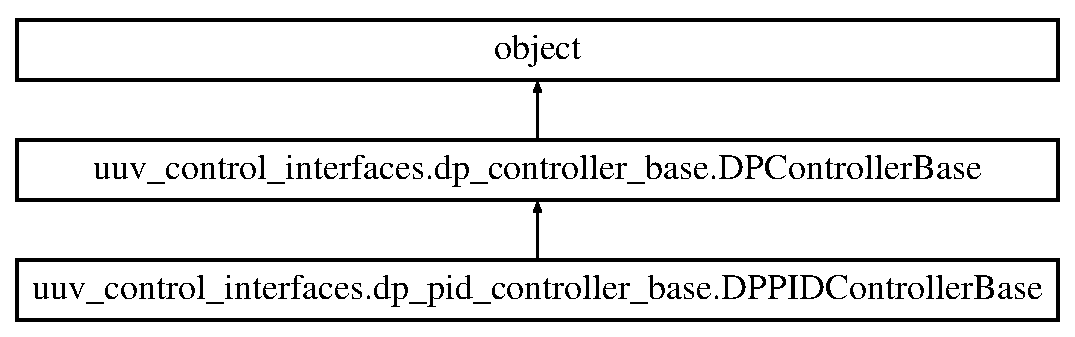
\includegraphics[height=3.000000cm]{classuuv__control__interfaces_1_1dp__pid__controller__base_1_1DPPIDControllerBase}
\end{center}
\end{figure}
\doxysubsection*{Public Member Functions}
\begin{DoxyCompactItemize}
\item 
\mbox{\Hypertarget{classuuv__control__interfaces_1_1dp__pid__controller__base_1_1DPPIDControllerBase_a04ea79c786b8099cdaed87f2dfd106ea}\label{classuuv__control__interfaces_1_1dp__pid__controller__base_1_1DPPIDControllerBase_a04ea79c786b8099cdaed87f2dfd106ea}} 
def {\bfseries \+\_\+\+\_\+init\+\_\+\+\_\+} (self, $\ast$args)
\item 
\mbox{\Hypertarget{classuuv__control__interfaces_1_1dp__pid__controller__base_1_1DPPIDControllerBase_aed2f924fb542ff14d9089f94e971bc57}\label{classuuv__control__interfaces_1_1dp__pid__controller__base_1_1DPPIDControllerBase_aed2f924fb542ff14d9089f94e971bc57}} 
def {\bfseries set\+\_\+pid\+\_\+params\+\_\+callback} (self, request)
\item 
\mbox{\Hypertarget{classuuv__control__interfaces_1_1dp__pid__controller__base_1_1DPPIDControllerBase_a0b48103803a42818aebe9ca7177fa4d5}\label{classuuv__control__interfaces_1_1dp__pid__controller__base_1_1DPPIDControllerBase_a0b48103803a42818aebe9ca7177fa4d5}} 
def {\bfseries get\+\_\+pid\+\_\+params\+\_\+callback} (self, request)
\item 
\mbox{\Hypertarget{classuuv__control__interfaces_1_1dp__pid__controller__base_1_1DPPIDControllerBase_aa2c44fa417cc560730ca270998a5c85b}\label{classuuv__control__interfaces_1_1dp__pid__controller__base_1_1DPPIDControllerBase_aa2c44fa417cc560730ca270998a5c85b}} 
def {\bfseries update\+\_\+pid} (self)
\end{DoxyCompactItemize}
\doxysubsection*{Additional Inherited Members}


\doxysubsection{Detailed Description}
\begin{DoxyVerb}This is an abstract class for PID-based controllers. The base class method
update_controller must be overridden in other for a controller to work.
\end{DoxyVerb}
 

The documentation for this class was generated from the following file\+:\begin{DoxyCompactItemize}
\item 
control\+\_\+layer/uuv\+\_\+trajectory\+\_\+control/src/uuv\+\_\+control\+\_\+interfaces/dp\+\_\+pid\+\_\+controller\+\_\+base.\+py\end{DoxyCompactItemize}

\hypertarget{classuuv__trajectory__generator_1_1path__generator_1_1dubins__interpolator_1_1DubinsInterpolator}{}\doxysection{uuv\+\_\+trajectory\+\_\+generator.\+path\+\_\+generator.\+dubins\+\_\+interpolator.\+Dubins\+Interpolator Class Reference}
\label{classuuv__trajectory__generator_1_1path__generator_1_1dubins__interpolator_1_1DubinsInterpolator}\index{uuv\_trajectory\_generator.path\_generator.dubins\_interpolator.DubinsInterpolator@{uuv\_trajectory\_generator.path\_generator.dubins\_interpolator.DubinsInterpolator}}
Inheritance diagram for uuv\+\_\+trajectory\+\_\+generator.\+path\+\_\+generator.\+dubins\+\_\+interpolator.\+Dubins\+Interpolator\+:\begin{figure}[H]
\begin{center}
\leavevmode
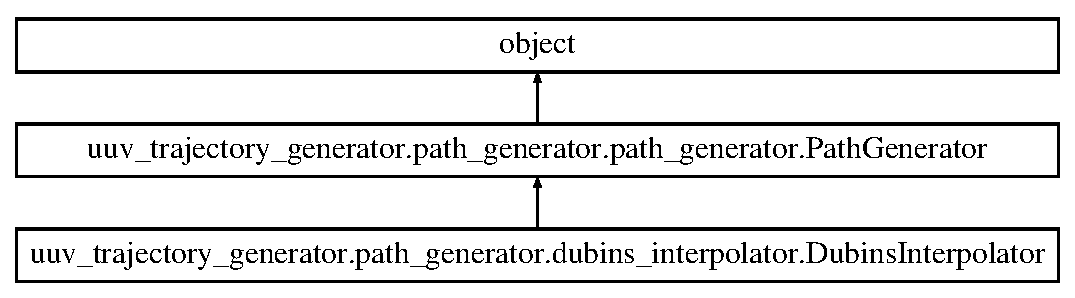
\includegraphics[height=3.000000cm]{classuuv__trajectory__generator_1_1path__generator_1_1dubins__interpolator_1_1DubinsInterpolator}
\end{center}
\end{figure}
\doxysubsection*{Public Member Functions}
\begin{DoxyCompactItemize}
\item 
\mbox{\Hypertarget{classuuv__trajectory__generator_1_1path__generator_1_1dubins__interpolator_1_1DubinsInterpolator_a9617766c385bbc3c0d7a16ed8694d17c}\label{classuuv__trajectory__generator_1_1path__generator_1_1dubins__interpolator_1_1DubinsInterpolator_a9617766c385bbc3c0d7a16ed8694d17c}} 
def {\bfseries \+\_\+\+\_\+init\+\_\+\+\_\+} (self)
\item 
\mbox{\Hypertarget{classuuv__trajectory__generator_1_1path__generator_1_1dubins__interpolator_1_1DubinsInterpolator_af4e03b47779f7388f4c06b2c3c9a0677}\label{classuuv__trajectory__generator_1_1path__generator_1_1dubins__interpolator_1_1DubinsInterpolator_af4e03b47779f7388f4c06b2c3c9a0677}} 
def {\bfseries init\+\_\+interpolator} (self)
\item 
\mbox{\Hypertarget{classuuv__trajectory__generator_1_1path__generator_1_1dubins__interpolator_1_1DubinsInterpolator_a4005bc913523b4540796110b27d25efc}\label{classuuv__trajectory__generator_1_1path__generator_1_1dubins__interpolator_1_1DubinsInterpolator_a4005bc913523b4540796110b27d25efc}} 
def {\bfseries set\+\_\+parameters} (self, params)
\item 
\mbox{\Hypertarget{classuuv__trajectory__generator_1_1path__generator_1_1dubins__interpolator_1_1DubinsInterpolator_a3326e407a715dfca02ae5ef90c1f9271}\label{classuuv__trajectory__generator_1_1path__generator_1_1dubins__interpolator_1_1DubinsInterpolator_a3326e407a715dfca02ae5ef90c1f9271}} 
def {\bfseries get\+\_\+samples} (self, max\+\_\+time, step=0.\+001)
\item 
\mbox{\Hypertarget{classuuv__trajectory__generator_1_1path__generator_1_1dubins__interpolator_1_1DubinsInterpolator_aa20c13496b4c2196169632a48f984e00}\label{classuuv__trajectory__generator_1_1path__generator_1_1dubins__interpolator_1_1DubinsInterpolator_aa20c13496b4c2196169632a48f984e00}} 
def {\bfseries generate\+\_\+pos} (self, s)
\item 
\mbox{\Hypertarget{classuuv__trajectory__generator_1_1path__generator_1_1dubins__interpolator_1_1DubinsInterpolator_a517bb22bea9b35466e61cf52ba224831}\label{classuuv__trajectory__generator_1_1path__generator_1_1dubins__interpolator_1_1DubinsInterpolator_a517bb22bea9b35466e61cf52ba224831}} 
def {\bfseries generate\+\_\+pnt} (self, s, t, $\ast$args)
\item 
\mbox{\Hypertarget{classuuv__trajectory__generator_1_1path__generator_1_1dubins__interpolator_1_1DubinsInterpolator_a7940350f5c244e433547a4d0235b7cf7}\label{classuuv__trajectory__generator_1_1path__generator_1_1dubins__interpolator_1_1DubinsInterpolator_a7940350f5c244e433547a4d0235b7cf7}} 
def {\bfseries generate\+\_\+quat} (self, s)
\end{DoxyCompactItemize}
\doxysubsection*{Static Public Attributes}
\begin{DoxyCompactItemize}
\item 
\mbox{\Hypertarget{classuuv__trajectory__generator_1_1path__generator_1_1dubins__interpolator_1_1DubinsInterpolator_aa447cb1a312ea49b9c85e07a2b9dff3c}\label{classuuv__trajectory__generator_1_1path__generator_1_1dubins__interpolator_1_1DubinsInterpolator_aa447cb1a312ea49b9c85e07a2b9dff3c}} 
string {\bfseries L\+A\+B\+EL} = \textquotesingle{}dubins\textquotesingle{}
\end{DoxyCompactItemize}
\doxysubsection*{Additional Inherited Members}


\doxysubsection{Detailed Description}
\begin{DoxyVerb}3D Dubins path interpolator
\end{DoxyVerb}
 

The documentation for this class was generated from the following file\+:\begin{DoxyCompactItemize}
\item 
control\+\_\+layer/uuv\+\_\+trajectory\+\_\+control/src/uuv\+\_\+trajectory\+\_\+generator/path\+\_\+generator/dubins\+\_\+interpolator.\+py\end{DoxyCompactItemize}

\hypertarget{structDVLData}{}\doxysection{D\+V\+L\+Data Struct Reference}
\label{structDVLData}\index{DVLData@{DVLData}}
\doxysubsection*{Public Attributes}
\begin{DoxyCompactItemize}
\item 
\mbox{\Hypertarget{structDVLData_a0c22a8518847aaa2e3a7b9ebddec7140}\label{structDVLData_a0c22a8518847aaa2e3a7b9ebddec7140}} 
unsigned char {\bfseries version}
\item 
\mbox{\Hypertarget{structDVLData_a0dcf730c3f314b8e9995f09271ea429f}\label{structDVLData_a0dcf730c3f314b8e9995f09271ea429f}} 
unsigned char {\bfseries offset\+Of\+Data}
\item 
\mbox{\Hypertarget{structDVLData_a52e5848fb99287368ad0197f9bbbf933}\label{structDVLData_a52e5848fb99287368ad0197f9bbbf933}} 
unsigned long {\bfseries serial\+Number}
\item 
\mbox{\Hypertarget{structDVLData_a7dbf5221a4979d8f9d9247b7de685ceb}\label{structDVLData_a7dbf5221a4979d8f9d9247b7de685ceb}} 
unsigned char {\bfseries year}
\item 
\mbox{\Hypertarget{structDVLData_a88bd22c3211688a07a9a2fa38f5920b8}\label{structDVLData_a88bd22c3211688a07a9a2fa38f5920b8}} 
unsigned char {\bfseries month}
\item 
\mbox{\Hypertarget{structDVLData_a9ed16962bfebc258033a99e0131c7acc}\label{structDVLData_a9ed16962bfebc258033a99e0131c7acc}} 
unsigned char {\bfseries day}
\item 
\mbox{\Hypertarget{structDVLData_ad850cc99098e5ce79835d0fe3f097526}\label{structDVLData_ad850cc99098e5ce79835d0fe3f097526}} 
unsigned char {\bfseries hour}
\item 
\mbox{\Hypertarget{structDVLData_a03deb0b38a326c68398a69b1fede89be}\label{structDVLData_a03deb0b38a326c68398a69b1fede89be}} 
unsigned char {\bfseries minute}
\item 
\mbox{\Hypertarget{structDVLData_a3839b3107d362771464c8cd0272e2273}\label{structDVLData_a3839b3107d362771464c8cd0272e2273}} 
unsigned char {\bfseries seconds}
\item 
\mbox{\Hypertarget{structDVLData_ac073304da623aa9e7eb1d2c9d9e40a18}\label{structDVLData_ac073304da623aa9e7eb1d2c9d9e40a18}} 
unsigned short {\bfseries micro\+Seconds100}
\item 
\mbox{\Hypertarget{structDVLData_a8d94c99a54c57ff87c5cee49fd8f5829}\label{structDVLData_a8d94c99a54c57ff87c5cee49fd8f5829}} 
unsigned short {\bfseries n\+Beams}
\item 
\mbox{\Hypertarget{structDVLData_a15ccb5e0614c789e3cb5ce91ad196e35}\label{structDVLData_a15ccb5e0614c789e3cb5ce91ad196e35}} 
unsigned long {\bfseries error}
\item 
\mbox{\Hypertarget{structDVLData_a77302e23f58411054cd2b6f4efd0d00f}\label{structDVLData_a77302e23f58411054cd2b6f4efd0d00f}} 
\mbox{\hyperlink{structDVLstatus}{D\+V\+Lstatus}} {\bfseries status}
\item 
\mbox{\Hypertarget{structDVLData_a4c9dfb379305a4f7f6320aa90bba9136}\label{structDVLData_a4c9dfb379305a4f7f6320aa90bba9136}} 
float {\bfseries sound\+Speed}
\item 
\mbox{\Hypertarget{structDVLData_aeafc0aefeea5f3faf94e963152d858e0}\label{structDVLData_aeafc0aefeea5f3faf94e963152d858e0}} 
float {\bfseries temperature}
\item 
\mbox{\Hypertarget{structDVLData_abb306335f258b6304b30a8434ed8b4d5}\label{structDVLData_abb306335f258b6304b30a8434ed8b4d5}} 
float {\bfseries pressure}
\item 
\mbox{\Hypertarget{structDVLData_a348fc03d2108f79d4fc4b7015c11a18b}\label{structDVLData_a348fc03d2108f79d4fc4b7015c11a18b}} 
float {\bfseries vel\+Beam} \mbox{[}4\mbox{]}
\item 
\mbox{\Hypertarget{structDVLData_ab6854b0ca2f1a66f29420d81886692fd}\label{structDVLData_ab6854b0ca2f1a66f29420d81886692fd}} 
float {\bfseries dist\+Beam} \mbox{[}4\mbox{]}
\item 
\mbox{\Hypertarget{structDVLData_a15058d6a00845d78993c945156e29448}\label{structDVLData_a15058d6a00845d78993c945156e29448}} 
float {\bfseries fom\+Beam} \mbox{[}4\mbox{]}
\item 
\mbox{\Hypertarget{structDVLData_ac89d99b327d991ac954e9fcfa6626571}\label{structDVLData_ac89d99b327d991ac954e9fcfa6626571}} 
float {\bfseries time\+Diff1\+Beam} \mbox{[}4\mbox{]}
\item 
\mbox{\Hypertarget{structDVLData_a28931909582a0c57a9dcbd1697bf02e4}\label{structDVLData_a28931909582a0c57a9dcbd1697bf02e4}} 
float {\bfseries time\+Diff2\+Beam} \mbox{[}4\mbox{]}
\item 
\mbox{\Hypertarget{structDVLData_af9258bf7e720912deec19759ca0fe5f5}\label{structDVLData_af9258bf7e720912deec19759ca0fe5f5}} 
float {\bfseries time\+Vel\+Est\+Beam} \mbox{[}4\mbox{]}
\item 
\mbox{\Hypertarget{structDVLData_a123caca46e2e4219ace9275cafef1cb0}\label{structDVLData_a123caca46e2e4219ace9275cafef1cb0}} 
float {\bfseries velX}
\item 
\mbox{\Hypertarget{structDVLData_a107d8e8cc0426eb3ef2f9f48ecb7297e}\label{structDVLData_a107d8e8cc0426eb3ef2f9f48ecb7297e}} 
float {\bfseries velY}
\item 
\mbox{\Hypertarget{structDVLData_a6278b4ceefa315241e9d4e7a6f899c58}\label{structDVLData_a6278b4ceefa315241e9d4e7a6f899c58}} 
float {\bfseries vel\+Z1}
\item 
\mbox{\Hypertarget{structDVLData_a1c7b313e86ceb53b97112e809910ec1e}\label{structDVLData_a1c7b313e86ceb53b97112e809910ec1e}} 
float {\bfseries vel\+Z2}
\item 
\mbox{\Hypertarget{structDVLData_ae1e29de62116777900f27d0b0f3cb1eb}\label{structDVLData_ae1e29de62116777900f27d0b0f3cb1eb}} 
float {\bfseries fomX}
\item 
\mbox{\Hypertarget{structDVLData_a3dfe66a48ae22bc2cceef656989dc6bf}\label{structDVLData_a3dfe66a48ae22bc2cceef656989dc6bf}} 
float {\bfseries fomY}
\item 
\mbox{\Hypertarget{structDVLData_a0f429d3af0b8fda07738ad1194c783d5}\label{structDVLData_a0f429d3af0b8fda07738ad1194c783d5}} 
float {\bfseries fom\+Z1}
\item 
\mbox{\Hypertarget{structDVLData_a5e3f75bb00ef3fbb164c8eda8ef51b4c}\label{structDVLData_a5e3f75bb00ef3fbb164c8eda8ef51b4c}} 
float {\bfseries fom\+Z2}
\item 
\mbox{\Hypertarget{structDVLData_a9676f7c3494bed0ec1d2610816d1837f}\label{structDVLData_a9676f7c3494bed0ec1d2610816d1837f}} 
float {\bfseries time\+Diff1X}
\item 
\mbox{\Hypertarget{structDVLData_a6c6102cc57797c0260e9df4b1000af67}\label{structDVLData_a6c6102cc57797c0260e9df4b1000af67}} 
float {\bfseries time\+Diff1Y}
\item 
\mbox{\Hypertarget{structDVLData_a4807a48d0a20c29c2c462e4991009627}\label{structDVLData_a4807a48d0a20c29c2c462e4991009627}} 
float {\bfseries time\+Diff1\+Z1}
\item 
\mbox{\Hypertarget{structDVLData_a4841e9f613f95b4dad3edd174fcb3c76}\label{structDVLData_a4841e9f613f95b4dad3edd174fcb3c76}} 
float {\bfseries time\+Diff1\+Z2}
\item 
\mbox{\Hypertarget{structDVLData_abcaade63338b5a467dda5acdbd8d45a6}\label{structDVLData_abcaade63338b5a467dda5acdbd8d45a6}} 
float {\bfseries time\+Diff2X}
\item 
\mbox{\Hypertarget{structDVLData_a42c34fe33fd7fa92e67e8c78fbfe9ad0}\label{structDVLData_a42c34fe33fd7fa92e67e8c78fbfe9ad0}} 
float {\bfseries time\+Diff2Y}
\item 
\mbox{\Hypertarget{structDVLData_a2fd590963df7f99255eb25cedddee0dd}\label{structDVLData_a2fd590963df7f99255eb25cedddee0dd}} 
float {\bfseries time\+Diff2\+Z1}
\item 
\mbox{\Hypertarget{structDVLData_ac0e9b12ec15d14692a60e63a4ac28bf6}\label{structDVLData_ac0e9b12ec15d14692a60e63a4ac28bf6}} 
float {\bfseries time\+Diff2\+Z2}
\item 
\mbox{\Hypertarget{structDVLData_a7cc2c76c6cdb0cc57917c3fc33e4a803}\label{structDVLData_a7cc2c76c6cdb0cc57917c3fc33e4a803}} 
float {\bfseries time\+Vel\+EstX}
\item 
\mbox{\Hypertarget{structDVLData_a3253ed16b2c8fc36d1f8897c67378975}\label{structDVLData_a3253ed16b2c8fc36d1f8897c67378975}} 
float {\bfseries time\+Vel\+EstY}
\item 
\mbox{\Hypertarget{structDVLData_a96d37886f690d7e7a757f1f2a021e92b}\label{structDVLData_a96d37886f690d7e7a757f1f2a021e92b}} 
float {\bfseries time\+Vel\+Est\+Z1}
\item 
\mbox{\Hypertarget{structDVLData_a6a63a73113c613b8f92caf59da3a41aa}\label{structDVLData_a6a63a73113c613b8f92caf59da3a41aa}} 
float {\bfseries time\+Vel\+Est\+Z2}
\end{DoxyCompactItemize}


The documentation for this struct was generated from the following file\+:\begin{DoxyCompactItemize}
\item 
hardware\+\_\+layer/hardware\+\_\+dvl\+\_\+ethernet/include/dvl\+\_\+data.\+h\end{DoxyCompactItemize}

\hypertarget{classnavigation_1_1DvlData}{}\doxysection{navigation\+::Dvl\+Data Class Reference}
\label{classnavigation_1_1DvlData}\index{navigation::DvlData@{navigation::DvlData}}
Inheritance diagram for navigation\+::Dvl\+Data\+:\begin{figure}[H]
\begin{center}
\leavevmode
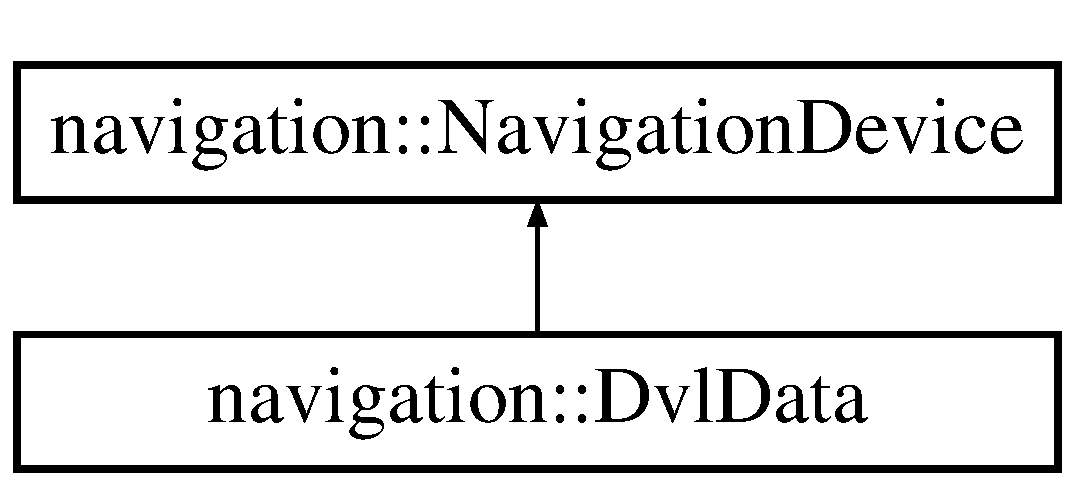
\includegraphics[height=2.000000cm]{classnavigation_1_1DvlData}
\end{center}
\end{figure}
\doxysubsection*{Public Types}
\begin{DoxyCompactItemize}
\item 
\mbox{\Hypertarget{classnavigation_1_1DvlData_ac24d2ec36fda2e666c6c1d99ea3b8f63}\label{classnavigation_1_1DvlData_ac24d2ec36fda2e666c6c1d99ea3b8f63}} 
enum {\bfseries Integration\+Method\+Type} \{ {\bfseries Std\+Method} = 0, 
{\bfseries R\+K\+Method}, 
{\bfseries Default\+Method}
 \}
\end{DoxyCompactItemize}
\doxysubsection*{Public Member Functions}
\begin{DoxyCompactItemize}
\item 
\mbox{\Hypertarget{classnavigation_1_1DvlData_a0869dc4d839aed3b0362e084f1f4f637}\label{classnavigation_1_1DvlData_a0869dc4d839aed3b0362e084f1f4f637}} 
{\bfseries Dvl\+Data} (Integration\+Method\+Type integration\+Method\+Type=R\+K\+Method)
\item 
\mbox{\Hypertarget{classnavigation_1_1DvlData_a3de3242a0cbea12329b09e266e900477}\label{classnavigation_1_1DvlData_a3de3242a0cbea12329b09e266e900477}} 
void {\bfseries Dvl\+Twist\+Callback} (geometry\+\_\+msgs\+::\+Twist\+With\+Covariance\+Stamped msg)
\item 
\mbox{\Hypertarget{classnavigation_1_1DvlData_ad8941460c960aadc7d995e2be367c8c8}\label{classnavigation_1_1DvlData_ad8941460c960aadc7d995e2be367c8c8}} 
void {\bfseries Dvl\+Pressure\+Callback} (std\+\_\+msgs\+::\+Float32 msg)
\item 
\mbox{\Hypertarget{classnavigation_1_1DvlData_adfcb95f8a4319806643b7c6e8e2c4a4a}\label{classnavigation_1_1DvlData_adfcb95f8a4319806643b7c6e8e2c4a4a}} 
Eigen\+::\+Vector3d {\bfseries Get\+Position\+X\+YZ} ()
\item 
\mbox{\Hypertarget{classnavigation_1_1DvlData_a39bab39003b8916544557a2ee6f20209}\label{classnavigation_1_1DvlData_a39bab39003b8916544557a2ee6f20209}} 
Eigen\+::\+Vector3d {\bfseries Get\+Velocity\+X\+YZ} ()
\item 
\mbox{\Hypertarget{classnavigation_1_1DvlData_a0fcf5be8a4f3393265351fffb810081b}\label{classnavigation_1_1DvlData_a0fcf5be8a4f3393265351fffb810081b}} 
double {\bfseries Get\+Position\+Z\+From\+Pressure} ()
\item 
\mbox{\Hypertarget{classnavigation_1_1DvlData_a54d3559339019627a33636157e369551}\label{classnavigation_1_1DvlData_a54d3559339019627a33636157e369551}} 
std\+\_\+msgs\+::\+Float32 {\bfseries Get\+Pressure} ()
\end{DoxyCompactItemize}
\doxysubsection*{Public Attributes}
\begin{DoxyCompactItemize}
\item 
\mbox{\Hypertarget{classnavigation_1_1DvlData_a2f08082395e159bb9e15a67c55f194dd}\label{classnavigation_1_1DvlData_a2f08082395e159bb9e15a67c55f194dd}} 
const double {\bfseries B\+A\+R\+\_\+\+T\+O\+\_\+\+M\+E\+T\+E\+R\+\_\+\+O\+F\+\_\+\+W\+A\+T\+ER} = 10.\+1972
\item 
\mbox{\Hypertarget{classnavigation_1_1DvlData_a249ba705a7eecd0e3cfa38c3ac0aaecf}\label{classnavigation_1_1DvlData_a249ba705a7eecd0e3cfa38c3ac0aaecf}} 
std\+::vector$<$ double $>$ {\bfseries x\+\_\+vel}
\item 
\mbox{\Hypertarget{classnavigation_1_1DvlData_a8e410bd105300614ceafe3a68c730c38}\label{classnavigation_1_1DvlData_a8e410bd105300614ceafe3a68c730c38}} 
std\+::vector$<$ double $>$ {\bfseries y\+\_\+vel}
\item 
\mbox{\Hypertarget{classnavigation_1_1DvlData_a30ad7a24b1d21eda7751fb9b39b70bcf}\label{classnavigation_1_1DvlData_a30ad7a24b1d21eda7751fb9b39b70bcf}} 
std\+::vector$<$ double $>$ {\bfseries z\+\_\+vel}
\item 
\mbox{\Hypertarget{classnavigation_1_1DvlData_a489d885d8b0604f091e95829a7850c5f}\label{classnavigation_1_1DvlData_a489d885d8b0604f091e95829a7850c5f}} 
int {\bfseries x\+\_\+count} = 0
\item 
\mbox{\Hypertarget{classnavigation_1_1DvlData_a5a4255a5ec33cb262f9b8f40d491b98a}\label{classnavigation_1_1DvlData_a5a4255a5ec33cb262f9b8f40d491b98a}} 
int {\bfseries y\+\_\+count} = 0
\item 
\mbox{\Hypertarget{classnavigation_1_1DvlData_a0a4e7896e814db0a042529d8a16b50d3}\label{classnavigation_1_1DvlData_a0a4e7896e814db0a042529d8a16b50d3}} 
int {\bfseries z\+\_\+count} = 0
\item 
\mbox{\Hypertarget{classnavigation_1_1DvlData_a4dd27495416fe948b07c4137574e0fed}\label{classnavigation_1_1DvlData_a4dd27495416fe948b07c4137574e0fed}} 
int {\bfseries vel\+\_\+count} = 0
\end{DoxyCompactItemize}


The documentation for this class was generated from the following files\+:\begin{DoxyCompactItemize}
\item 
navigation\+\_\+layer/odom\+\_\+dvl\+\_\+imu/include/dvl\+\_\+data.\+h\item 
navigation\+\_\+layer/odom\+\_\+dvl\+\_\+imu/src/dvl\+\_\+data.\+cpp\end{DoxyCompactItemize}

\hypertarget{classDVLEthernet}{}\section{D\+V\+L\+Ethernet Class Reference}
\label{classDVLEthernet}\index{D\+V\+L\+Ethernet@{D\+V\+L\+Ethernet}}
\subsection*{Public Member Functions}
\begin{DoxyCompactItemize}
\item 
\mbox{\Hypertarget{classDVLEthernet_ad30402a8fe0eb3c717d77b2eed7084c1}\label{classDVLEthernet_ad30402a8fe0eb3c717d77b2eed7084c1}} 
void {\bfseries Connect} (std\+::string address, int port)
\item 
\mbox{\Hypertarget{classDVLEthernet_a3e9002198a62dbf53a5cd0e590915a1d}\label{classDVLEthernet_a3e9002198a62dbf53a5cd0e590915a1d}} 
void {\bfseries Receive} ()
\item 
\mbox{\Hypertarget{classDVLEthernet_a9d797679645c1944672d4e94b415bfd0}\label{classDVLEthernet_a9d797679645c1944672d4e94b415bfd0}} 
char $\ast$ {\bfseries Get\+Raw\+Data} ()
\end{DoxyCompactItemize}


The documentation for this class was generated from the following files\+:\begin{DoxyCompactItemize}
\item 
hardware\+\_\+layer/hardware\+\_\+dvl\+\_\+ethernet/include/dvl\+\_\+ethernet.\+h\item 
hardware\+\_\+layer/hardware\+\_\+dvl\+\_\+ethernet/src/driver/dvl\+\_\+ethernet.\+cpp\end{DoxyCompactItemize}

\hypertarget{structDVLformat21__t}{}\section{D\+V\+Lformat21\+\_\+t Struct Reference}
\label{structDVLformat21__t}\index{D\+V\+Lformat21\+\_\+t@{D\+V\+Lformat21\+\_\+t}}
\subsection*{Public Attributes}
\begin{DoxyCompactItemize}
\item 
\mbox{\Hypertarget{structDVLformat21__t_a73ccb6a2f243fcb72d17fb50b0f06268}\label{structDVLformat21__t_a73ccb6a2f243fcb72d17fb50b0f06268}} 
\hyperlink{structDVLHeader}{D\+V\+L\+Header} {\bfseries header}
\item 
\mbox{\Hypertarget{structDVLformat21__t_aadedba2c0c9ae4ba1207402182b1039c}\label{structDVLformat21__t_aadedba2c0c9ae4ba1207402182b1039c}} 
\hyperlink{structDVLData}{D\+V\+L\+Data} {\bfseries data}
\end{DoxyCompactItemize}


The documentation for this struct was generated from the following file\+:\begin{DoxyCompactItemize}
\item 
hardware\+\_\+layer/hardware\+\_\+dvl\+\_\+ethernet/include/dvl\+\_\+data.\+h\end{DoxyCompactItemize}

\hypertarget{structDVLHeader}{}\section{D\+V\+L\+Header Struct Reference}
\label{structDVLHeader}\index{D\+V\+L\+Header@{D\+V\+L\+Header}}
\subsection*{Public Attributes}
\begin{DoxyCompactItemize}
\item 
\mbox{\Hypertarget{structDVLHeader_a27d0ac6baf29d0559ead2a9384b1dded}\label{structDVLHeader_a27d0ac6baf29d0559ead2a9384b1dded}} 
unsigned char {\bfseries sync}
\item 
\mbox{\Hypertarget{structDVLHeader_a2c42e3db97f1529bd582b6f7d2ce18aa}\label{structDVLHeader_a2c42e3db97f1529bd582b6f7d2ce18aa}} 
unsigned char {\bfseries hdr\+Size}
\item 
\mbox{\Hypertarget{structDVLHeader_af2ca0a3aad38abdb1ce53783596b9949}\label{structDVLHeader_af2ca0a3aad38abdb1ce53783596b9949}} 
unsigned char {\bfseries ID}
\item 
\mbox{\Hypertarget{structDVLHeader_a3cb5d36f47a1a70d4ed4095ff367369f}\label{structDVLHeader_a3cb5d36f47a1a70d4ed4095ff367369f}} 
unsigned char {\bfseries family}
\item 
\mbox{\Hypertarget{structDVLHeader_a9b3d0692b86e568dc9994736f5bbd000}\label{structDVLHeader_a9b3d0692b86e568dc9994736f5bbd000}} 
unsigned short {\bfseries data\+Size}
\item 
\mbox{\Hypertarget{structDVLHeader_a7221731a16a8856930a7346e613016a4}\label{structDVLHeader_a7221731a16a8856930a7346e613016a4}} 
unsigned short {\bfseries data\+Checksum}
\item 
\mbox{\Hypertarget{structDVLHeader_a5bb58b3b0829d51dd65833b7c6a7da77}\label{structDVLHeader_a5bb58b3b0829d51dd65833b7c6a7da77}} 
unsigned short {\bfseries hdr\+Checksum}
\end{DoxyCompactItemize}


The documentation for this struct was generated from the following file\+:\begin{DoxyCompactItemize}
\item 
hardware\+\_\+layer/hardware\+\_\+dvl\+\_\+ethernet/include/dvl\+\_\+data.\+h\end{DoxyCompactItemize}

\hypertarget{classhardware__dvl_1_1DVLNode}{}\doxysection{hardware\+\_\+dvl\+::D\+V\+L\+Node Class Reference}
\label{classhardware__dvl_1_1DVLNode}\index{hardware\_dvl::DVLNode@{hardware\_dvl::DVLNode}}
\doxysubsection*{Public Member Functions}
\begin{DoxyCompactItemize}
\item 
\mbox{\Hypertarget{classhardware__dvl_1_1DVLNode_aa91c4da13e96fd56c72efba5c17bce21}\label{classhardware__dvl_1_1DVLNode_aa91c4da13e96fd56c72efba5c17bce21}} 
{\bfseries D\+V\+L\+Node} (const ros\+::\+Node\+Handle\+Ptr \&nh)
\item 
\mbox{\Hypertarget{classhardware__dvl_1_1DVLNode_abf3be4e29c2226d6e37e3cbb25e11909}\label{classhardware__dvl_1_1DVLNode_abf3be4e29c2226d6e37e3cbb25e11909}} 
void {\bfseries Spin} ()
\end{DoxyCompactItemize}


The documentation for this class was generated from the following files\+:\begin{DoxyCompactItemize}
\item 
hardware\+\_\+layer/hardware\+\_\+dvl\+\_\+ethernet/include/dvl\+\_\+connection.\+h\item 
hardware\+\_\+layer/hardware\+\_\+dvl\+\_\+ethernet/src/hardware\+\_\+dvl\+\_\+ethernet/dvl\+\_\+connection.\+cpp\end{DoxyCompactItemize}

\hypertarget{structDVLstatus}{}\doxysection{D\+V\+Lstatus Struct Reference}
\label{structDVLstatus}\index{DVLstatus@{DVLstatus}}
\doxysubsection*{Public Attributes}
\begin{DoxyCompactItemize}
\item 
\mbox{\Hypertarget{structDVLstatus_a405f7663cad8090b27f9e215c7db6fe9}\label{structDVLstatus_a405f7663cad8090b27f9e215c7db6fe9}} 
unsigned long {\bfseries beam1\+Vel\+Valid}\+: 1
\item 
\mbox{\Hypertarget{structDVLstatus_a53978a4d789e5c1c65139d05b2e1263c}\label{structDVLstatus_a53978a4d789e5c1c65139d05b2e1263c}} 
unsigned long {\bfseries beam2\+Vel\+Valid}\+: 1
\item 
\mbox{\Hypertarget{structDVLstatus_a495d0e27c2f604b3f8952a3198cab411}\label{structDVLstatus_a495d0e27c2f604b3f8952a3198cab411}} 
unsigned long {\bfseries beam3\+Vel\+Valid}\+: 1
\item 
\mbox{\Hypertarget{structDVLstatus_a85a7800693b0147eee214658d0c8c510}\label{structDVLstatus_a85a7800693b0147eee214658d0c8c510}} 
unsigned long {\bfseries beam4\+Vel\+Valid}\+: 1
\item 
\mbox{\Hypertarget{structDVLstatus_af046590caa5844f63acc79fd0871526d}\label{structDVLstatus_af046590caa5844f63acc79fd0871526d}} 
unsigned long {\bfseries beam1\+Dist\+Valid}\+: 1
\item 
\mbox{\Hypertarget{structDVLstatus_ad7b1de7455cd6c44cf3d2d14f2f05951}\label{structDVLstatus_ad7b1de7455cd6c44cf3d2d14f2f05951}} 
unsigned long {\bfseries beam2\+Dist\+Valid}\+: 1
\item 
\mbox{\Hypertarget{structDVLstatus_aab61f47a41140ce1469eea7daaa5d4b2}\label{structDVLstatus_aab61f47a41140ce1469eea7daaa5d4b2}} 
unsigned long {\bfseries beam3\+Dist\+Valid}\+: 1
\item 
\mbox{\Hypertarget{structDVLstatus_a367e8d056ba9c2aadf924621bfc6d040}\label{structDVLstatus_a367e8d056ba9c2aadf924621bfc6d040}} 
unsigned long {\bfseries beam4\+Dist\+Valid}\+: 1
\item 
\mbox{\Hypertarget{structDVLstatus_ad1c234d1bad1c320a8ba6681dd865f9b}\label{structDVLstatus_ad1c234d1bad1c320a8ba6681dd865f9b}} 
unsigned long {\bfseries beam1\+F\+O\+M\+Valid}\+: 1
\item 
\mbox{\Hypertarget{structDVLstatus_adad506a00cb45fc81ee00ba011a4b7e6}\label{structDVLstatus_adad506a00cb45fc81ee00ba011a4b7e6}} 
unsigned long {\bfseries beam2\+F\+O\+M\+Valid}\+: 1
\item 
\mbox{\Hypertarget{structDVLstatus_a5f6bb4f2ebda804ed0de4799f524bfe4}\label{structDVLstatus_a5f6bb4f2ebda804ed0de4799f524bfe4}} 
unsigned long {\bfseries beam3\+F\+O\+M\+Valid}\+: 1
\item 
\mbox{\Hypertarget{structDVLstatus_a3a60760fc8a41108746737c1b2b9a1fc}\label{structDVLstatus_a3a60760fc8a41108746737c1b2b9a1fc}} 
unsigned long {\bfseries beam4\+F\+O\+M\+Valid}\+: 1
\item 
\mbox{\Hypertarget{structDVLstatus_a7897fab4708c27414d930fa1a02f83e7}\label{structDVLstatus_a7897fab4708c27414d930fa1a02f83e7}} 
unsigned long {\bfseries x\+Vel\+Valid}\+: 1
\item 
\mbox{\Hypertarget{structDVLstatus_aa41af34ce95e6bb38a5957c313215b68}\label{structDVLstatus_aa41af34ce95e6bb38a5957c313215b68}} 
unsigned long {\bfseries y\+Vel\+Valid}\+: 1
\item 
\mbox{\Hypertarget{structDVLstatus_a15a9a1e1f9b0a96fc2620b0f619ccf9c}\label{structDVLstatus_a15a9a1e1f9b0a96fc2620b0f619ccf9c}} 
unsigned long {\bfseries z1\+Vel\+Valid}\+: 1
\item 
\mbox{\Hypertarget{structDVLstatus_ae169438e5ad27ec3895adeaa3873e48b}\label{structDVLstatus_ae169438e5ad27ec3895adeaa3873e48b}} 
unsigned long {\bfseries z2\+Vel\+Valid}\+: 1
\item 
\mbox{\Hypertarget{structDVLstatus_ab609b50a6660dc016ff2c56b2a344345}\label{structDVLstatus_ab609b50a6660dc016ff2c56b2a344345}} 
unsigned long {\bfseries x\+F\+O\+M\+Valid}\+: 1
\item 
\mbox{\Hypertarget{structDVLstatus_ada4eebc4f3444a268e408597b3e1e4e4}\label{structDVLstatus_ada4eebc4f3444a268e408597b3e1e4e4}} 
unsigned long {\bfseries y\+F\+O\+M\+Valid}\+: 1
\item 
\mbox{\Hypertarget{structDVLstatus_a12f80ecfa3dd831b5b37f5ad6a8fa91f}\label{structDVLstatus_a12f80ecfa3dd831b5b37f5ad6a8fa91f}} 
unsigned long {\bfseries z1\+F\+O\+M\+Valid}\+: 1
\item 
\mbox{\Hypertarget{structDVLstatus_a7c73c07a1a7357aa119bad7a798be13d}\label{structDVLstatus_a7c73c07a1a7357aa119bad7a798be13d}} 
unsigned long {\bfseries z2\+F\+O\+M\+Valid}\+: 1
\item 
\mbox{\Hypertarget{structDVLstatus_af3cf7c19ed56065095b69325d9a45d64}\label{structDVLstatus_af3cf7c19ed56065095b69325d9a45d64}} 
unsigned long {\bfseries proc\+Idle3}\+: 1
\item 
\mbox{\Hypertarget{structDVLstatus_a1f37cf4fe49c9e75e7d558514e3df69e}\label{structDVLstatus_a1f37cf4fe49c9e75e7d558514e3df69e}} 
unsigned long {\bfseries proc\+Idle6}\+: 1
\item 
\mbox{\Hypertarget{structDVLstatus_a6a93208697cce85f8bf509bc138668f2}\label{structDVLstatus_a6a93208697cce85f8bf509bc138668f2}} 
unsigned long {\bfseries proc\+Idle12}\+: 1
\item 
\mbox{\Hypertarget{structDVLstatus_a88cdaf75532d8e9b4a866c1e1505bf22}\label{structDVLstatus_a88cdaf75532d8e9b4a866c1e1505bf22}} 
unsigned long {\bfseries \+\_\+empty1}\+: 5
\item 
\mbox{\Hypertarget{structDVLstatus_a732333bfd4d841915d049961e860cc91}\label{structDVLstatus_a732333bfd4d841915d049961e860cc91}} 
unsigned long {\bfseries wakeupstate}\+: 4
\end{DoxyCompactItemize}


The documentation for this struct was generated from the following file\+:\begin{DoxyCompactItemize}
\item 
hardware\+\_\+layer/hardware\+\_\+dvl\+\_\+ethernet/include/dvl\+\_\+data.\+h\end{DoxyCompactItemize}

\hypertarget{classmapping_1_1EKF}{}\section{mapping\+:\+:E\+KF$<$ n, m, b $>$ Class Template Reference}
\label{classmapping_1_1EKF}\index{mapping\+::\+E\+K\+F$<$ n, m, b $>$@{mapping\+::\+E\+K\+F$<$ n, m, b $>$}}
\subsection*{Public Member Functions}
\begin{DoxyCompactItemize}
\item 
\mbox{\Hypertarget{classmapping_1_1EKF_a7cd0997810543b9bcd1b7507c394141a}\label{classmapping_1_1EKF_a7cd0997810543b9bcd1b7507c394141a}} 
{\bfseries E\+KF} (const Eigen\+::\+Matrix$<$ float, n, b $>$ \&B, const Eigen\+::\+Matrix$<$ float, m, m $>$ \&R, const Eigen\+::\+Matrix$<$ float, n, n $>$ \&Q, const Eigen\+::\+Matrix$<$ float, n, 1 $>$ \&x, const Eigen\+::\+Matrix$<$ float, n, n $>$ \&p)
\item 
\mbox{\Hypertarget{classmapping_1_1EKF_afd006c8edcaec96df002a017d7088709}\label{classmapping_1_1EKF_afd006c8edcaec96df002a017d7088709}} 
void {\bfseries Predict} (const Eigen\+::\+Matrix$<$ float, b, 1 $>$ \&u, const Eigen\+::\+Matrix$<$ float, n, 1 $>$ \&xhat, const Eigen\+::\+Matrix$<$ float, n, n $>$ \&F)
\item 
\mbox{\Hypertarget{classmapping_1_1EKF_a890e40b9407dbd02acbdea2a9d520060}\label{classmapping_1_1EKF_a890e40b9407dbd02acbdea2a9d520060}} 
void {\bfseries Update} (const Eigen\+::\+Matrix$<$ float, m, 1 $>$ \&y, const Eigen\+::\+Matrix$<$ float, m, n $>$ \&H)
\item 
\mbox{\Hypertarget{classmapping_1_1EKF_a7cd0997810543b9bcd1b7507c394141a}\label{classmapping_1_1EKF_a7cd0997810543b9bcd1b7507c394141a}} 
{\bfseries E\+KF} (const Eigen\+::\+Matrix$<$ float, n, b $>$ \&B, const Eigen\+::\+Matrix$<$ float, m, m $>$ \&R, const Eigen\+::\+Matrix$<$ float, n, n $>$ \&Q, const Eigen\+::\+Matrix$<$ float, n, 1 $>$ \&x, const Eigen\+::\+Matrix$<$ float, n, n $>$ \&p)
\item 
\mbox{\Hypertarget{classmapping_1_1EKF_afd006c8edcaec96df002a017d7088709}\label{classmapping_1_1EKF_afd006c8edcaec96df002a017d7088709}} 
void {\bfseries Predict} (const Eigen\+::\+Matrix$<$ float, b, 1 $>$ \&u, const Eigen\+::\+Matrix$<$ float, n, 1 $>$ \&xhat, const Eigen\+::\+Matrix$<$ float, n, n $>$ \&F)
\item 
\mbox{\Hypertarget{classmapping_1_1EKF_a890e40b9407dbd02acbdea2a9d520060}\label{classmapping_1_1EKF_a890e40b9407dbd02acbdea2a9d520060}} 
void {\bfseries Update} (const Eigen\+::\+Matrix$<$ float, m, 1 $>$ \&y, const Eigen\+::\+Matrix$<$ float, m, n $>$ \&H)
\end{DoxyCompactItemize}
\subsection*{Public Attributes}
\begin{DoxyCompactItemize}
\item 
\mbox{\Hypertarget{classmapping_1_1EKF_af953a8e0f00fb0afd7ea402e47748c66}\label{classmapping_1_1EKF_af953a8e0f00fb0afd7ea402e47748c66}} 
Eigen\+::\+Matrix$<$ float, n, 1 $>$ {\bfseries xhat\+\_\+}
\item 
\mbox{\Hypertarget{classmapping_1_1EKF_ad782328cf17a9ef5cae9028802603b9f}\label{classmapping_1_1EKF_ad782328cf17a9ef5cae9028802603b9f}} 
Eigen\+::\+Matrix$<$ float, n, n $>$ {\bfseries covs\+\_\+}
\end{DoxyCompactItemize}
\subsection*{Protected Attributes}
\begin{DoxyCompactItemize}
\item 
\mbox{\Hypertarget{classmapping_1_1EKF_a1c2cf3acfc47603a2c89b18079ea958a}\label{classmapping_1_1EKF_a1c2cf3acfc47603a2c89b18079ea958a}} 
Eigen\+::\+Matrix$<$ float, n, b $>$ {\bfseries B\+\_\+}
\item 
\mbox{\Hypertarget{classmapping_1_1EKF_a5e9f13b5188a461f973518b398d6bd52}\label{classmapping_1_1EKF_a5e9f13b5188a461f973518b398d6bd52}} 
Eigen\+::\+Matrix$<$ float, m, m $>$ {\bfseries R\+\_\+}
\item 
\mbox{\Hypertarget{classmapping_1_1EKF_a276acb331f3fd0c5aeeb2d6b0711d4eb}\label{classmapping_1_1EKF_a276acb331f3fd0c5aeeb2d6b0711d4eb}} 
Eigen\+::\+Matrix$<$ float, n, n $>$ {\bfseries Q\+\_\+}
\end{DoxyCompactItemize}


The documentation for this class was generated from the following files\+:\begin{DoxyCompactItemize}
\item 
navigation\+\_\+layer/mapping/include/ekf.\+h\item 
navigation\+\_\+layer/mapping/include/slam\+\_\+ekf.\+h\item 
navigation\+\_\+layer/mapping/src/ekf.\+cpp\end{DoxyCompactItemize}

\hypertarget{classErrorDescriptor}{}\doxysection{Error\+Descriptor Class Reference}
\label{classErrorDescriptor}\index{ErrorDescriptor@{ErrorDescriptor}}
\doxysubsection*{Public Member Functions}
\begin{DoxyCompactItemize}
\item 
\mbox{\Hypertarget{classErrorDescriptor_aa6873020ab6b06ed818163e21b32153d}\label{classErrorDescriptor_aa6873020ab6b06ed818163e21b32153d}} 
{\bfseries Error\+Descriptor} (std\+::string \+\_\+name)
\item 
\mbox{\Hypertarget{classErrorDescriptor_afc783570c3d68c62484d3d497c63611b}\label{classErrorDescriptor_afc783570c3d68c62484d3d497c63611b}} 
void {\bfseries set\+P\+ID} (float new\+\_\+p, float new\+\_\+i, float new\+\_\+d, float new\+\_\+band)
\item 
\mbox{\Hypertarget{classErrorDescriptor_a7843bd233c7fadd26654a42c8c447911}\label{classErrorDescriptor_a7843bd233c7fadd26654a42c8c447911}} 
void {\bfseries set\+Type} (std\+::string \+\_\+name)
\item 
\mbox{\Hypertarget{classErrorDescriptor_ab4bf6a37278e571abc09da8327625fd3}\label{classErrorDescriptor_ab4bf6a37278e571abc09da8327625fd3}} 
void {\bfseries set\+Reference} (double \+\_\+value)
\item 
\mbox{\Hypertarget{classErrorDescriptor_ac461f29a6baa8cbfda296d39e12fafb3}\label{classErrorDescriptor_ac461f29a6baa8cbfda296d39e12fafb3}} 
void {\bfseries error\+To\+P\+WM} (double \+\_\+current\+\_\+value)
\item 
\mbox{\Hypertarget{classErrorDescriptor_a0092487859383d38d70a2cf4c67cb42f}\label{classErrorDescriptor_a0092487859383d38d70a2cf4c67cb42f}} 
int {\bfseries get\+P\+WM} ()
\item 
\mbox{\Hypertarget{classErrorDescriptor_aae79d462e543e29c61b5267558f4bdc4}\label{classErrorDescriptor_aae79d462e543e29c61b5267558f4bdc4}} 
double {\bfseries get\+Current\+Value} ()
\end{DoxyCompactItemize}


The documentation for this class was generated from the following files\+:\begin{DoxyCompactItemize}
\item 
debug\+\_\+layer/pid\+\_\+calibration/include/pid\+\_\+calibration/error\+To\+P\+W\+M.\+h\item 
debug\+\_\+layer/pid\+\_\+calibration/src/error\+To\+P\+W\+M.\+cpp\end{DoxyCompactItemize}

\hypertarget{classnavigation_1_1ExtendedKalmanFilter}{}\doxysection{navigation\+::Extended\+Kalman\+Filter Class Reference}
\label{classnavigation_1_1ExtendedKalmanFilter}\index{navigation::ExtendedKalmanFilter@{navigation::ExtendedKalmanFilter}}
\doxysubsection*{Public Member Functions}
\begin{DoxyCompactItemize}
\item 
\mbox{\Hypertarget{classnavigation_1_1ExtendedKalmanFilter_aa2e08d1aac6aa0abe3226d223688f6cb}\label{classnavigation_1_1ExtendedKalmanFilter_aa2e08d1aac6aa0abe3226d223688f6cb}} 
void {\bfseries Update} (Eigen\+::\+Vector3d \&measurement, Eigen\+::\+Vector3d \&estimation)
\item 
\mbox{\Hypertarget{classnavigation_1_1ExtendedKalmanFilter_acc5c4a9358d53a4198bb1aa15b7e8b91}\label{classnavigation_1_1ExtendedKalmanFilter_acc5c4a9358d53a4198bb1aa15b7e8b91}} 
void {\bfseries Initialization} (float pval, float qval, float rval)
\end{DoxyCompactItemize}


The documentation for this class was generated from the following files\+:\begin{DoxyCompactItemize}
\item 
navigation\+\_\+layer/odom\+\_\+dvl\+\_\+imu/include/ekf.\+h\item 
navigation\+\_\+layer/odom\+\_\+dvl\+\_\+imu/src/ekf.\+cpp\end{DoxyCompactItemize}

\hypertarget{classvision__commons_1_1Filter}{}\doxysection{vision\+\_\+commons\+::Filter Class Reference}
\label{classvision__commons_1_1Filter}\index{vision\_commons::Filter@{vision\_commons::Filter}}
\doxysubsection*{Static Public Member Functions}
\begin{DoxyCompactItemize}
\item 
\mbox{\Hypertarget{classvision__commons_1_1Filter_a54fcd78039a49ff9d0b323013052219b}\label{classvision__commons_1_1Filter_a54fcd78039a49ff9d0b323013052219b}} 
static cv\+::\+Mat {\bfseries clahe} (cv\+::\+Mat \&image, double clahe\+\_\+clip, int clahe\+\_\+grid\+\_\+size)
\item 
\mbox{\Hypertarget{classvision__commons_1_1Filter_a372a71db1d4802c610ad7aae69ab325f}\label{classvision__commons_1_1Filter_a372a71db1d4802c610ad7aae69ab325f}} 
static cv\+::\+Mat {\bfseries balance\+\_\+white} (cv\+::\+Mat \&image)
\item 
\mbox{\Hypertarget{classvision__commons_1_1Filter_ae111029e3b0f4fe991af1edcf1393310}\label{classvision__commons_1_1Filter_ae111029e3b0f4fe991af1edcf1393310}} 
static cv\+::\+Mat {\bfseries blue\+\_\+filter} (cv\+::\+Mat \&image, double clahe\+\_\+clip, int clahe\+\_\+grid\+\_\+size, int clahe\+\_\+bilateral\+\_\+iter, int balanced\+\_\+bilateral\+\_\+iter, double denoise\+\_\+h)
\item 
\mbox{\Hypertarget{classvision__commons_1_1Filter_ab12e10894d0272f7add8c77638000c78}\label{classvision__commons_1_1Filter_ab12e10894d0272f7add8c77638000c78}} 
static void {\bfseries bilateral} (cv\+::\+Mat \&src, int iterations)
\end{DoxyCompactItemize}


The documentation for this class was generated from the following files\+:\begin{DoxyCompactItemize}
\item 
vision\+\_\+layer/vision\+\_\+commons/include/filter.\+h\item 
vision\+\_\+layer/vision\+\_\+commons/src/filter.\+cpp\end{DoxyCompactItemize}

\hypertarget{classmaster__layer_1_1state__mach_1_1FindBottomTarget}{}\doxysection{master\+\_\+layer.\+state\+\_\+mach.\+Find\+Bottom\+Target Class Reference}
\label{classmaster__layer_1_1state__mach_1_1FindBottomTarget}\index{master\_layer.state\_mach.FindBottomTarget@{master\_layer.state\_mach.FindBottomTarget}}
Inheritance diagram for master\+\_\+layer.\+state\+\_\+mach.\+Find\+Bottom\+Target\+:\begin{figure}[H]
\begin{center}
\leavevmode
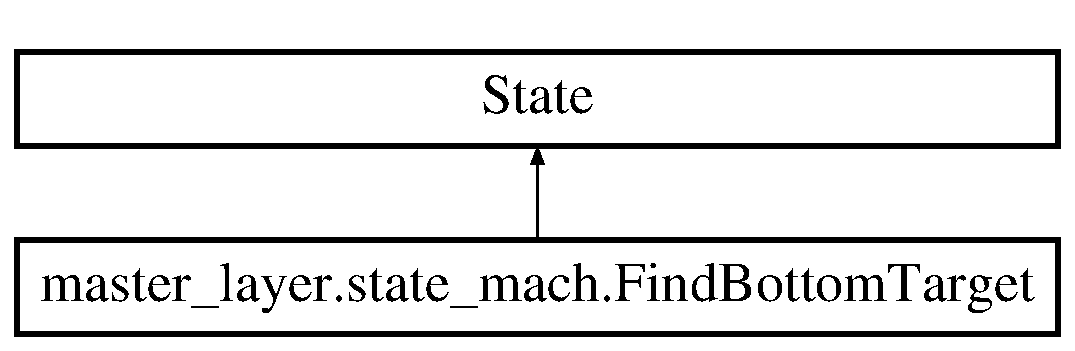
\includegraphics[height=2.000000cm]{classmaster__layer_1_1state__mach_1_1FindBottomTarget}
\end{center}
\end{figure}
\doxysubsection*{Public Member Functions}
\begin{DoxyCompactItemize}
\item 
\mbox{\Hypertarget{classmaster__layer_1_1state__mach_1_1FindBottomTarget_affe3849f49224418c92b861a1f8caf5d}\label{classmaster__layer_1_1state__mach_1_1FindBottomTarget_affe3849f49224418c92b861a1f8caf5d}} 
def {\bfseries \+\_\+\+\_\+init\+\_\+\+\_\+} (self)
\item 
\mbox{\Hypertarget{classmaster__layer_1_1state__mach_1_1FindBottomTarget_a7d98a6e5387914c6f52bdd19e3957225}\label{classmaster__layer_1_1state__mach_1_1FindBottomTarget_a7d98a6e5387914c6f52bdd19e3957225}} 
def {\bfseries execute} (self, userdata)
\item 
\mbox{\Hypertarget{classmaster__layer_1_1state__mach_1_1FindBottomTarget_a80a644d8358eb0732241072b3ad50f45}\label{classmaster__layer_1_1state__mach_1_1FindBottomTarget_a80a644d8358eb0732241072b3ad50f45}} 
def {\bfseries explore} (self)
\end{DoxyCompactItemize}


The documentation for this class was generated from the following file\+:\begin{DoxyCompactItemize}
\item 
master\+\_\+layer/src/master\+\_\+layer/state\+\_\+mach.\+py\end{DoxyCompactItemize}

\hypertarget{classmaster__layer_1_1state__mach__gate__torpedo_1_1FindBottomTarget}{}\section{master\+\_\+layer.\+state\+\_\+mach\+\_\+gate\+\_\+torpedo.\+Find\+Bottom\+Target Class Reference}
\label{classmaster__layer_1_1state__mach__gate__torpedo_1_1FindBottomTarget}\index{master\+\_\+layer.\+state\+\_\+mach\+\_\+gate\+\_\+torpedo.\+Find\+Bottom\+Target@{master\+\_\+layer.\+state\+\_\+mach\+\_\+gate\+\_\+torpedo.\+Find\+Bottom\+Target}}
Inheritance diagram for master\+\_\+layer.\+state\+\_\+mach\+\_\+gate\+\_\+torpedo.\+Find\+Bottom\+Target\+:\begin{figure}[H]
\begin{center}
\leavevmode
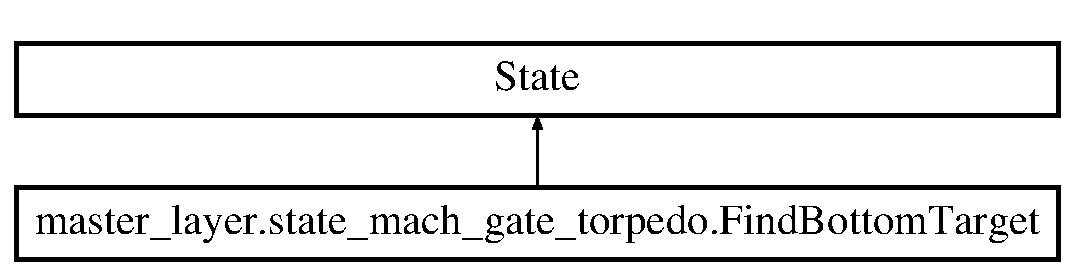
\includegraphics[height=2.000000cm]{classmaster__layer_1_1state__mach__gate__torpedo_1_1FindBottomTarget}
\end{center}
\end{figure}
\subsection*{Public Member Functions}
\begin{DoxyCompactItemize}
\item 
\mbox{\Hypertarget{classmaster__layer_1_1state__mach__gate__torpedo_1_1FindBottomTarget_a4c424b735499dad966149d0d4283d38c}\label{classmaster__layer_1_1state__mach__gate__torpedo_1_1FindBottomTarget_a4c424b735499dad966149d0d4283d38c}} 
def {\bfseries \+\_\+\+\_\+init\+\_\+\+\_\+} (self)
\item 
\mbox{\Hypertarget{classmaster__layer_1_1state__mach__gate__torpedo_1_1FindBottomTarget_a7f403b40fc74567ddf667ba2c896d573}\label{classmaster__layer_1_1state__mach__gate__torpedo_1_1FindBottomTarget_a7f403b40fc74567ddf667ba2c896d573}} 
def {\bfseries execute} (self, userdata)
\item 
\mbox{\Hypertarget{classmaster__layer_1_1state__mach__gate__torpedo_1_1FindBottomTarget_a84607cff814b0e32d122578bf00b701a}\label{classmaster__layer_1_1state__mach__gate__torpedo_1_1FindBottomTarget_a84607cff814b0e32d122578bf00b701a}} 
def {\bfseries explore} (self)
\end{DoxyCompactItemize}


The documentation for this class was generated from the following file\+:\begin{DoxyCompactItemize}
\item 
master\+\_\+layer/src/master\+\_\+layer/state\+\_\+mach\+\_\+gate\+\_\+torpedo.\+py\end{DoxyCompactItemize}

\hypertarget{classmaster__layer_1_1state__mach_1_1FindFrontTarget}{}\doxysection{master\+\_\+layer.\+state\+\_\+mach.\+Find\+Front\+Target Class Reference}
\label{classmaster__layer_1_1state__mach_1_1FindFrontTarget}\index{master\_layer.state\_mach.FindFrontTarget@{master\_layer.state\_mach.FindFrontTarget}}
Inheritance diagram for master\+\_\+layer.\+state\+\_\+mach.\+Find\+Front\+Target\+:\begin{figure}[H]
\begin{center}
\leavevmode
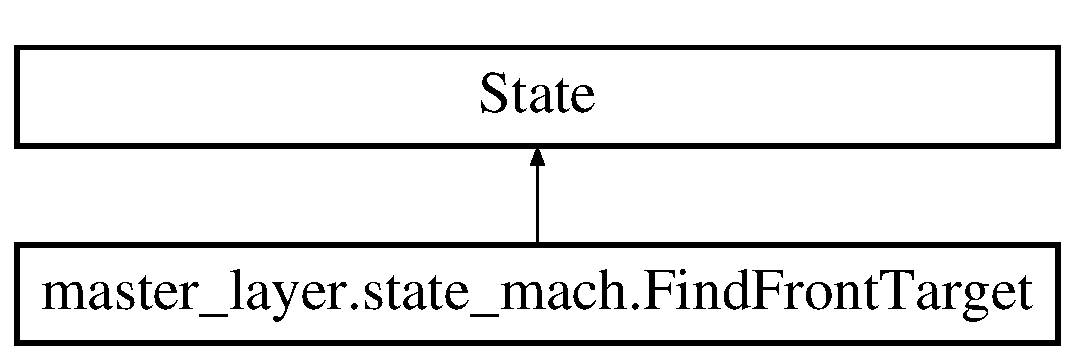
\includegraphics[height=2.000000cm]{classmaster__layer_1_1state__mach_1_1FindFrontTarget}
\end{center}
\end{figure}
\doxysubsection*{Public Member Functions}
\begin{DoxyCompactItemize}
\item 
\mbox{\Hypertarget{classmaster__layer_1_1state__mach_1_1FindFrontTarget_ad1d5a3483204ec88731ac498a7650bb0}\label{classmaster__layer_1_1state__mach_1_1FindFrontTarget_ad1d5a3483204ec88731ac498a7650bb0}} 
def {\bfseries \+\_\+\+\_\+init\+\_\+\+\_\+} (self)
\item 
\mbox{\Hypertarget{classmaster__layer_1_1state__mach_1_1FindFrontTarget_a4778c27a63368bb9700f2d87dc77a474}\label{classmaster__layer_1_1state__mach_1_1FindFrontTarget_a4778c27a63368bb9700f2d87dc77a474}} 
def {\bfseries conventional\+\_\+detector\+\_\+cb} (self, msg)
\item 
\mbox{\Hypertarget{classmaster__layer_1_1state__mach_1_1FindFrontTarget_afe5a90f3d8b4c7fa03add79337438274}\label{classmaster__layer_1_1state__mach_1_1FindFrontTarget_afe5a90f3d8b4c7fa03add79337438274}} 
def {\bfseries ml\+\_\+cb} (self, msg)
\item 
\mbox{\Hypertarget{classmaster__layer_1_1state__mach_1_1FindFrontTarget_a4a89a085e91502fd35a72f4bc2722cb1}\label{classmaster__layer_1_1state__mach_1_1FindFrontTarget_a4a89a085e91502fd35a72f4bc2722cb1}} 
def {\bfseries odometry\+\_\+callback} (self, msg)
\item 
\mbox{\Hypertarget{classmaster__layer_1_1state__mach_1_1FindFrontTarget_ae9a3b4cbeb328b614e2c573ab32ef1fd}\label{classmaster__layer_1_1state__mach_1_1FindFrontTarget_ae9a3b4cbeb328b614e2c573ab32ef1fd}} 
def {\bfseries has\+\_\+reached\+\_\+with\+\_\+yaw} (self, target\+\_\+pose, curr\+\_\+pose, pos\+\_\+threshold, yaw\+\_\+threshold)
\item 
\mbox{\Hypertarget{classmaster__layer_1_1state__mach_1_1FindFrontTarget_abc13a9a78656f54508b7d819c6fe53c4}\label{classmaster__layer_1_1state__mach_1_1FindFrontTarget_abc13a9a78656f54508b7d819c6fe53c4}} 
def {\bfseries execute} (self)
\item 
\mbox{\Hypertarget{classmaster__layer_1_1state__mach_1_1FindFrontTarget_a9f77b7e45c5850fe2f2d4e7388c227b7}\label{classmaster__layer_1_1state__mach_1_1FindFrontTarget_a9f77b7e45c5850fe2f2d4e7388c227b7}} 
def {\bfseries explore} (self)
\end{DoxyCompactItemize}


The documentation for this class was generated from the following file\+:\begin{DoxyCompactItemize}
\item 
master\+\_\+layer/src/master\+\_\+layer/state\+\_\+mach.\+py\end{DoxyCompactItemize}

\hypertarget{classmaster__layer_1_1state__mach__gate__torpedo_1_1FindFrontTarget}{}\section{master\+\_\+layer.\+state\+\_\+mach\+\_\+gate\+\_\+torpedo.\+Find\+Front\+Target Class Reference}
\label{classmaster__layer_1_1state__mach__gate__torpedo_1_1FindFrontTarget}\index{master\+\_\+layer.\+state\+\_\+mach\+\_\+gate\+\_\+torpedo.\+Find\+Front\+Target@{master\+\_\+layer.\+state\+\_\+mach\+\_\+gate\+\_\+torpedo.\+Find\+Front\+Target}}
Inheritance diagram for master\+\_\+layer.\+state\+\_\+mach\+\_\+gate\+\_\+torpedo.\+Find\+Front\+Target\+:\begin{figure}[H]
\begin{center}
\leavevmode
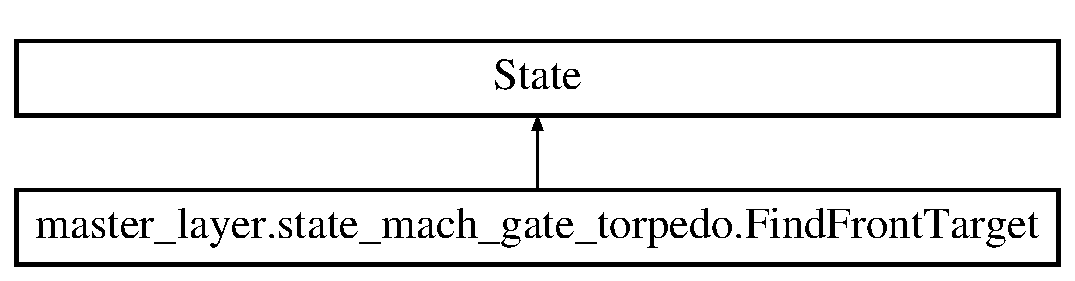
\includegraphics[height=2.000000cm]{classmaster__layer_1_1state__mach__gate__torpedo_1_1FindFrontTarget}
\end{center}
\end{figure}
\subsection*{Public Member Functions}
\begin{DoxyCompactItemize}
\item 
\mbox{\Hypertarget{classmaster__layer_1_1state__mach__gate__torpedo_1_1FindFrontTarget_a5999bc8b157a7eb9b2046b87ea66f990}\label{classmaster__layer_1_1state__mach__gate__torpedo_1_1FindFrontTarget_a5999bc8b157a7eb9b2046b87ea66f990}} 
def {\bfseries \+\_\+\+\_\+init\+\_\+\+\_\+} (self)
\item 
\mbox{\Hypertarget{classmaster__layer_1_1state__mach__gate__torpedo_1_1FindFrontTarget_a77c6dc67b18e3f3978dae9c381351896}\label{classmaster__layer_1_1state__mach__gate__torpedo_1_1FindFrontTarget_a77c6dc67b18e3f3978dae9c381351896}} 
def {\bfseries conventional\+\_\+detector\+\_\+cb} (self, msg)
\item 
\mbox{\Hypertarget{classmaster__layer_1_1state__mach__gate__torpedo_1_1FindFrontTarget_a743f11be402bf922c16c0aec04c43e6e}\label{classmaster__layer_1_1state__mach__gate__torpedo_1_1FindFrontTarget_a743f11be402bf922c16c0aec04c43e6e}} 
def {\bfseries ml\+\_\+cb} (self, msg)
\item 
\mbox{\Hypertarget{classmaster__layer_1_1state__mach__gate__torpedo_1_1FindFrontTarget_a2598c83f422342a85fe61e171dab9df2}\label{classmaster__layer_1_1state__mach__gate__torpedo_1_1FindFrontTarget_a2598c83f422342a85fe61e171dab9df2}} 
def {\bfseries odometry\+\_\+callback} (self, msg)
\item 
\mbox{\Hypertarget{classmaster__layer_1_1state__mach__gate__torpedo_1_1FindFrontTarget_ac034453b57d1d9c8e51d874d0583e25b}\label{classmaster__layer_1_1state__mach__gate__torpedo_1_1FindFrontTarget_ac034453b57d1d9c8e51d874d0583e25b}} 
def {\bfseries has\+\_\+reached\+\_\+with\+\_\+yaw} (self, target\+\_\+pose, curr\+\_\+pose, pos\+\_\+threshold, yaw\+\_\+threshold)
\item 
\mbox{\Hypertarget{classmaster__layer_1_1state__mach__gate__torpedo_1_1FindFrontTarget_a6f5ae668a1813a92c70476ed5612e818}\label{classmaster__layer_1_1state__mach__gate__torpedo_1_1FindFrontTarget_a6f5ae668a1813a92c70476ed5612e818}} 
def {\bfseries execute} (self)
\item 
\mbox{\Hypertarget{classmaster__layer_1_1state__mach__gate__torpedo_1_1FindFrontTarget_acd1897be61b181a9949df89f59bc64f4}\label{classmaster__layer_1_1state__mach__gate__torpedo_1_1FindFrontTarget_acd1897be61b181a9949df89f59bc64f4}} 
def {\bfseries explore} (self)
\end{DoxyCompactItemize}


The documentation for this class was generated from the following file\+:\begin{DoxyCompactItemize}
\item 
master\+\_\+layer/src/master\+\_\+layer/state\+\_\+mach\+\_\+gate\+\_\+torpedo.\+py\end{DoxyCompactItemize}

\hypertarget{classuuv__auv__actuator__interface_1_1fin__model_1_1FinModel}{}\section{uuv\+\_\+auv\+\_\+actuator\+\_\+interface.\+fin\+\_\+model.\+Fin\+Model Class Reference}
\label{classuuv__auv__actuator__interface_1_1fin__model_1_1FinModel}\index{uuv\+\_\+auv\+\_\+actuator\+\_\+interface.\+fin\+\_\+model.\+Fin\+Model@{uuv\+\_\+auv\+\_\+actuator\+\_\+interface.\+fin\+\_\+model.\+Fin\+Model}}
Inheritance diagram for uuv\+\_\+auv\+\_\+actuator\+\_\+interface.\+fin\+\_\+model.\+Fin\+Model\+:\begin{figure}[H]
\begin{center}
\leavevmode
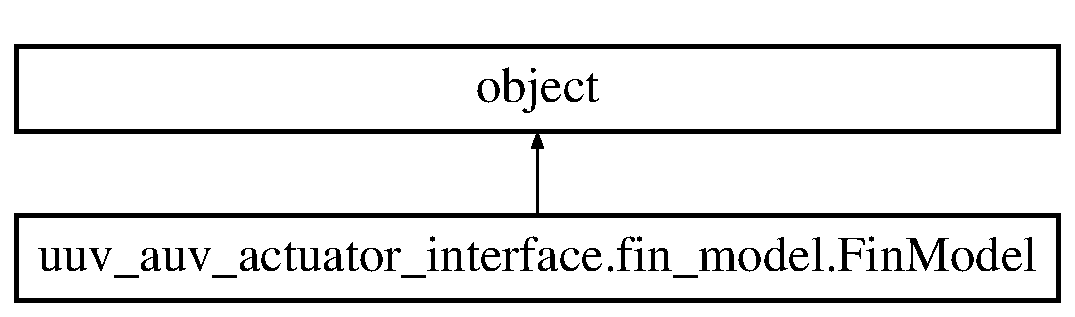
\includegraphics[height=2.000000cm]{classuuv__auv__actuator__interface_1_1fin__model_1_1FinModel}
\end{center}
\end{figure}
\subsection*{Public Member Functions}
\begin{DoxyCompactItemize}
\item 
\mbox{\Hypertarget{classuuv__auv__actuator__interface_1_1fin__model_1_1FinModel_a00749152250af4a7a5619d1184510267}\label{classuuv__auv__actuator__interface_1_1fin__model_1_1FinModel_a00749152250af4a7a5619d1184510267}} 
def {\bfseries \+\_\+\+\_\+init\+\_\+\+\_\+} (self, index, pos, quat, topic)
\item 
\mbox{\Hypertarget{classuuv__auv__actuator__interface_1_1fin__model_1_1FinModel_a406855fc9e43497eabbf022e848d202b}\label{classuuv__auv__actuator__interface_1_1fin__model_1_1FinModel_a406855fc9e43497eabbf022e848d202b}} 
def {\bfseries publish\+\_\+command} (self, delta)
\end{DoxyCompactItemize}
\subsection*{Public Attributes}
\begin{DoxyCompactItemize}
\item 
\mbox{\Hypertarget{classuuv__auv__actuator__interface_1_1fin__model_1_1FinModel_adb2d671adfee20ff82cb43c1a696384c}\label{classuuv__auv__actuator__interface_1_1fin__model_1_1FinModel_adb2d671adfee20ff82cb43c1a696384c}} 
{\bfseries id}
\item 
\mbox{\Hypertarget{classuuv__auv__actuator__interface_1_1fin__model_1_1FinModel_aa1b8c3a221069fb8d9c2485d2685c07c}\label{classuuv__auv__actuator__interface_1_1fin__model_1_1FinModel_aa1b8c3a221069fb8d9c2485d2685c07c}} 
{\bfseries pos}
\item 
\mbox{\Hypertarget{classuuv__auv__actuator__interface_1_1fin__model_1_1FinModel_ab8d1a9dd20e3f1a0468b902e9facaf89}\label{classuuv__auv__actuator__interface_1_1fin__model_1_1FinModel_ab8d1a9dd20e3f1a0468b902e9facaf89}} 
{\bfseries quat}
\item 
\mbox{\Hypertarget{classuuv__auv__actuator__interface_1_1fin__model_1_1FinModel_a182765f56abc7234d74c0406712bef0b}\label{classuuv__auv__actuator__interface_1_1fin__model_1_1FinModel_a182765f56abc7234d74c0406712bef0b}} 
{\bfseries topic}
\item 
\mbox{\Hypertarget{classuuv__auv__actuator__interface_1_1fin__model_1_1FinModel_a8b81e3ce36f9718d10fad74518fbc066}\label{classuuv__auv__actuator__interface_1_1fin__model_1_1FinModel_a8b81e3ce36f9718d10fad74518fbc066}} 
{\bfseries rot}
\item 
\mbox{\Hypertarget{classuuv__auv__actuator__interface_1_1fin__model_1_1FinModel_a496c22a608b6b8405366f276130f57d9}\label{classuuv__auv__actuator__interface_1_1fin__model_1_1FinModel_a496c22a608b6b8405366f276130f57d9}} 
{\bfseries lift\+\_\+vector}
\item 
\mbox{\Hypertarget{classuuv__auv__actuator__interface_1_1fin__model_1_1FinModel_a7de2f1459a2f8ca5b12d24f414508150}\label{classuuv__auv__actuator__interface_1_1fin__model_1_1FinModel_a7de2f1459a2f8ca5b12d24f414508150}} 
{\bfseries drag\+\_\+vector}
\item 
\mbox{\Hypertarget{classuuv__auv__actuator__interface_1_1fin__model_1_1FinModel_aace8499fc4475f553f393b1217d2eb4a}\label{classuuv__auv__actuator__interface_1_1fin__model_1_1FinModel_aace8499fc4475f553f393b1217d2eb4a}} 
{\bfseries pub}
\end{DoxyCompactItemize}


The documentation for this class was generated from the following file\+:\begin{DoxyCompactItemize}
\item 
control\+\_\+layer/uuv\+\_\+auv\+\_\+control\+\_\+allocator/src/uuv\+\_\+auv\+\_\+actuator\+\_\+interface/fin\+\_\+model.\+py\end{DoxyCompactItemize}

\hypertarget{classGate}{}\section{Gate Class Reference}
\label{classGate}\index{Gate@{Gate}}
Inheritance diagram for Gate\+:\begin{figure}[H]
\begin{center}
\leavevmode
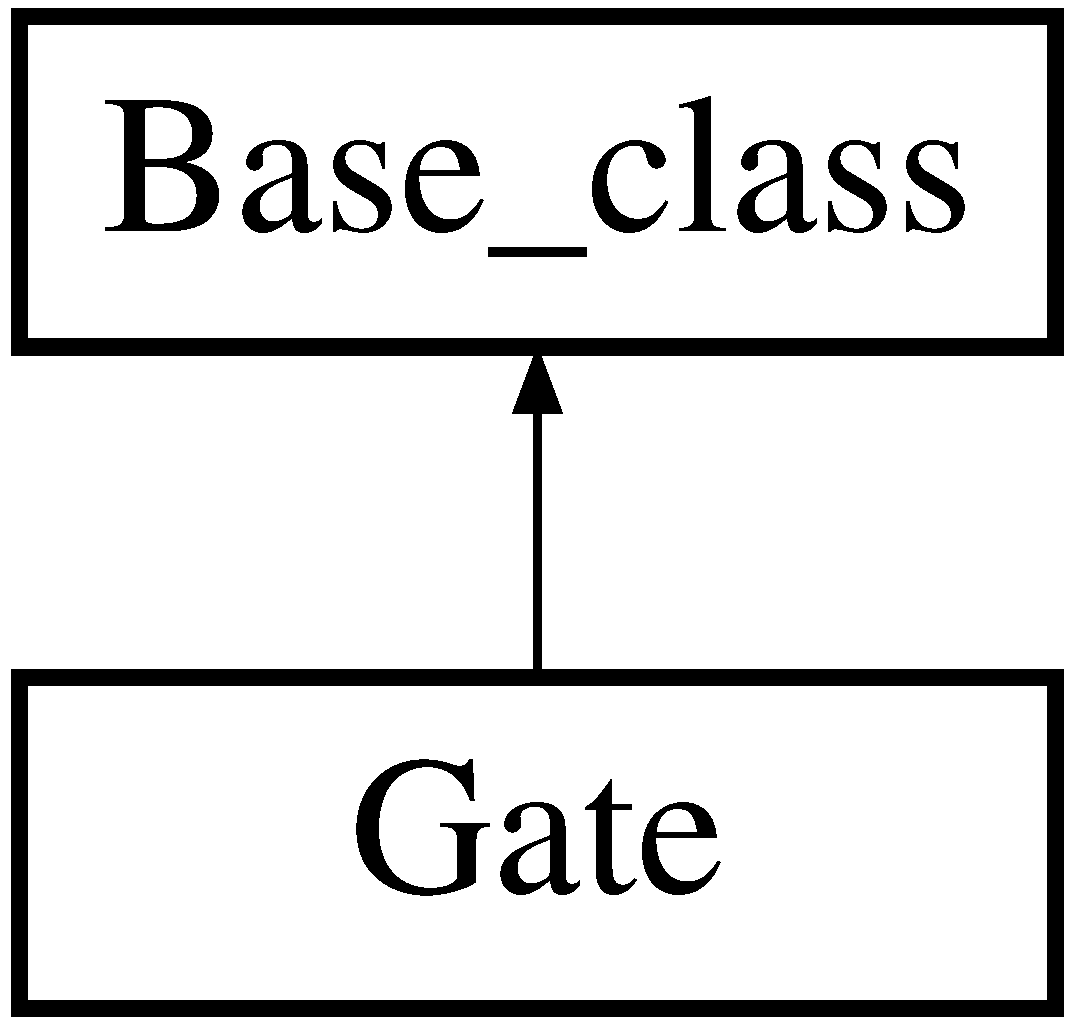
\includegraphics[height=2.000000cm]{classGate}
\end{center}
\end{figure}
\subsection*{Public Member Functions}
\begin{DoxyCompactItemize}
\item 
\mbox{\Hypertarget{classGate_a84014be339079ee8c26e5c627cf74172}\label{classGate_a84014be339079ee8c26e5c627cf74172}} 
void {\bfseries load\+Params} () override
\item 
\mbox{\Hypertarget{classGate_a91e5885a819d7155f4ee660126f0dc7e}\label{classGate_a91e5885a819d7155f4ee660126f0dc7e}} 
void {\bfseries spin\+Thread\+Front} () override
\end{DoxyCompactItemize}
\subsection*{Additional Inherited Members}


The documentation for this class was generated from the following files\+:\begin{DoxyCompactItemize}
\item 
vision\+\_\+layer/vision\+\_\+tasks/include/gate.\+h\item 
vision\+\_\+layer/vision\+\_\+tasks/src/gate.\+cpp\end{DoxyCompactItemize}

\hypertarget{classmaster__layer_1_1state__mach__gate__torpedo_1_1GateTask}{}\section{master\+\_\+layer.\+state\+\_\+mach\+\_\+gate\+\_\+torpedo.\+Gate\+Task Class Reference}
\label{classmaster__layer_1_1state__mach__gate__torpedo_1_1GateTask}\index{master\+\_\+layer.\+state\+\_\+mach\+\_\+gate\+\_\+torpedo.\+Gate\+Task@{master\+\_\+layer.\+state\+\_\+mach\+\_\+gate\+\_\+torpedo.\+Gate\+Task}}
Inheritance diagram for master\+\_\+layer.\+state\+\_\+mach\+\_\+gate\+\_\+torpedo.\+Gate\+Task\+:\begin{figure}[H]
\begin{center}
\leavevmode
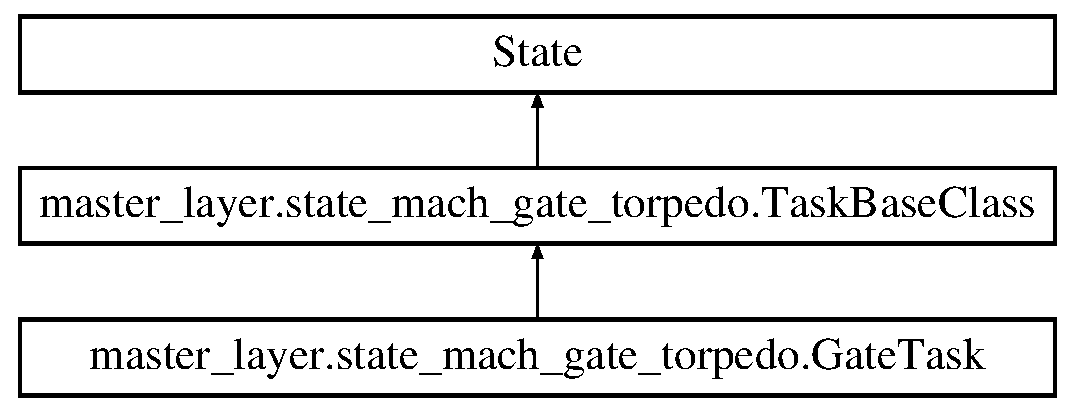
\includegraphics[height=3.000000cm]{classmaster__layer_1_1state__mach__gate__torpedo_1_1GateTask}
\end{center}
\end{figure}
\subsection*{Public Member Functions}
\begin{DoxyCompactItemize}
\item 
\mbox{\Hypertarget{classmaster__layer_1_1state__mach__gate__torpedo_1_1GateTask_a61b799fcb1c3add55187a4bc631929cd}\label{classmaster__layer_1_1state__mach__gate__torpedo_1_1GateTask_a61b799fcb1c3add55187a4bc631929cd}} 
def {\bfseries \+\_\+\+\_\+init\+\_\+\+\_\+} (self)
\item 
\mbox{\Hypertarget{classmaster__layer_1_1state__mach__gate__torpedo_1_1GateTask_ad837696bba16c665b25497aa76717eae}\label{classmaster__layer_1_1state__mach__gate__torpedo_1_1GateTask_ad837696bba16c665b25497aa76717eae}} 
def {\bfseries wait\+\_\+for\+\_\+crossing} (self)
\item 
\mbox{\Hypertarget{classmaster__layer_1_1state__mach__gate__torpedo_1_1GateTask_a9439565557a79294e004e6a63de032d7}\label{classmaster__layer_1_1state__mach__gate__torpedo_1_1GateTask_a9439565557a79294e004e6a63de032d7}} 
def {\bfseries move\+\_\+forward} (self)
\item 
\mbox{\Hypertarget{classmaster__layer_1_1state__mach__gate__torpedo_1_1GateTask_aca1234ad1e776c9d0e251ea20e0d5633}\label{classmaster__layer_1_1state__mach__gate__torpedo_1_1GateTask_aca1234ad1e776c9d0e251ea20e0d5633}} 
def {\bfseries execute} (self)
\end{DoxyCompactItemize}


The documentation for this class was generated from the following file\+:\begin{DoxyCompactItemize}
\item 
master\+\_\+layer/src/master\+\_\+layer/state\+\_\+mach\+\_\+gate\+\_\+torpedo.\+py\end{DoxyCompactItemize}

\hypertarget{classmaster__layer_1_1state__mach_1_1GateTask}{}\doxysection{master\+\_\+layer.\+state\+\_\+mach.\+Gate\+Task Class Reference}
\label{classmaster__layer_1_1state__mach_1_1GateTask}\index{master\_layer.state\_mach.GateTask@{master\_layer.state\_mach.GateTask}}
Inheritance diagram for master\+\_\+layer.\+state\+\_\+mach.\+Gate\+Task\+:\begin{figure}[H]
\begin{center}
\leavevmode
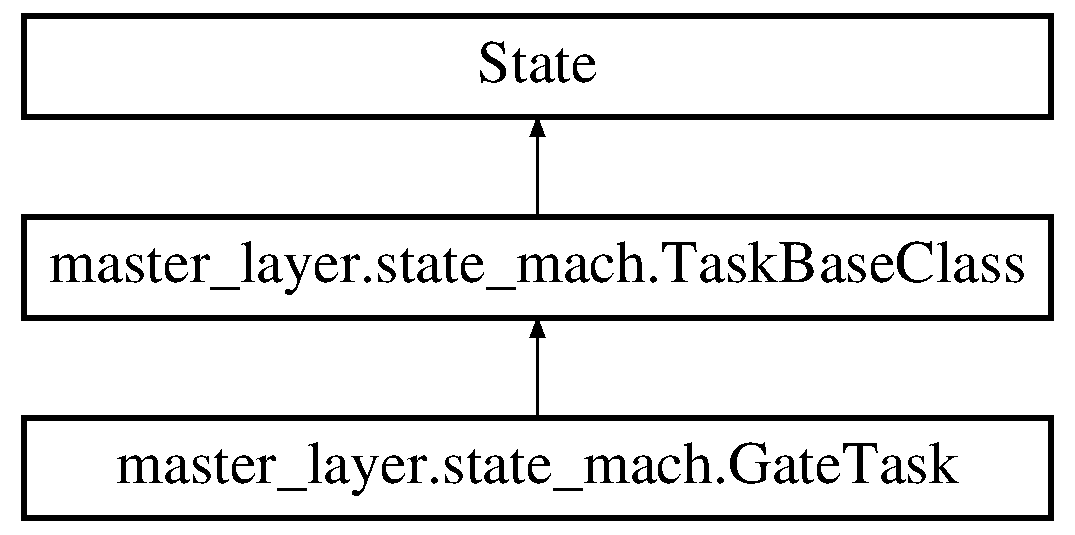
\includegraphics[height=3.000000cm]{classmaster__layer_1_1state__mach_1_1GateTask}
\end{center}
\end{figure}
\doxysubsection*{Public Member Functions}
\begin{DoxyCompactItemize}
\item 
\mbox{\Hypertarget{classmaster__layer_1_1state__mach_1_1GateTask_a9b03103ec10e1e177fd898d94f456bd9}\label{classmaster__layer_1_1state__mach_1_1GateTask_a9b03103ec10e1e177fd898d94f456bd9}} 
def {\bfseries \+\_\+\+\_\+init\+\_\+\+\_\+} (self)
\item 
\mbox{\Hypertarget{classmaster__layer_1_1state__mach_1_1GateTask_a186ab7679ee691a49b2cdd4e15394ce9}\label{classmaster__layer_1_1state__mach_1_1GateTask_a186ab7679ee691a49b2cdd4e15394ce9}} 
def {\bfseries wait\+\_\+for\+\_\+crossing} (self)
\item 
\mbox{\Hypertarget{classmaster__layer_1_1state__mach_1_1GateTask_a5b76b2e464f2a805683430f963039337}\label{classmaster__layer_1_1state__mach_1_1GateTask_a5b76b2e464f2a805683430f963039337}} 
def {\bfseries move\+\_\+forward} (self)
\item 
\mbox{\Hypertarget{classmaster__layer_1_1state__mach_1_1GateTask_afe32c860e9f85192bd584aba2868e3c4}\label{classmaster__layer_1_1state__mach_1_1GateTask_afe32c860e9f85192bd584aba2868e3c4}} 
def {\bfseries execute} (self)
\end{DoxyCompactItemize}


The documentation for this class was generated from the following file\+:\begin{DoxyCompactItemize}
\item 
master\+\_\+layer/src/master\+\_\+layer/state\+\_\+mach.\+py\end{DoxyCompactItemize}

\hypertarget{classvision__commons_1_1Geometry}{}\doxysection{vision\+\_\+commons\+::Geometry Class Reference}
\label{classvision__commons_1_1Geometry}\index{vision\_commons::Geometry@{vision\_commons::Geometry}}
\doxysubsection*{Static Public Member Functions}
\begin{DoxyCompactItemize}
\item 
\mbox{\Hypertarget{classvision__commons_1_1Geometry_aa3787f4923df9b302c4ddc780fa357cc}\label{classvision__commons_1_1Geometry_aa3787f4923df9b302c4ddc780fa357cc}} 
static double {\bfseries distance} (cv\+::\+Point \&p1, cv\+::\+Point \&p2)
\item 
\mbox{\Hypertarget{classvision__commons_1_1Geometry_a1576d1ef96bf4e57a8e132715c8be2bd}\label{classvision__commons_1_1Geometry_a1576d1ef96bf4e57a8e132715c8be2bd}} 
static double {\bfseries angle\+WrtY} (cv\+::\+Point \&p1, cv\+::\+Point \&p2)
\end{DoxyCompactItemize}


The documentation for this class was generated from the following files\+:\begin{DoxyCompactItemize}
\item 
vision\+\_\+layer/vision\+\_\+commons/include/geometry.\+h\item 
vision\+\_\+layer/vision\+\_\+commons/src/geometry.\+cpp\end{DoxyCompactItemize}

\hypertarget{classGrabber}{}\section{Grabber Class Reference}
\label{classGrabber}\index{Grabber@{Grabber}}
Inheritance diagram for Grabber\+:\begin{figure}[H]
\begin{center}
\leavevmode
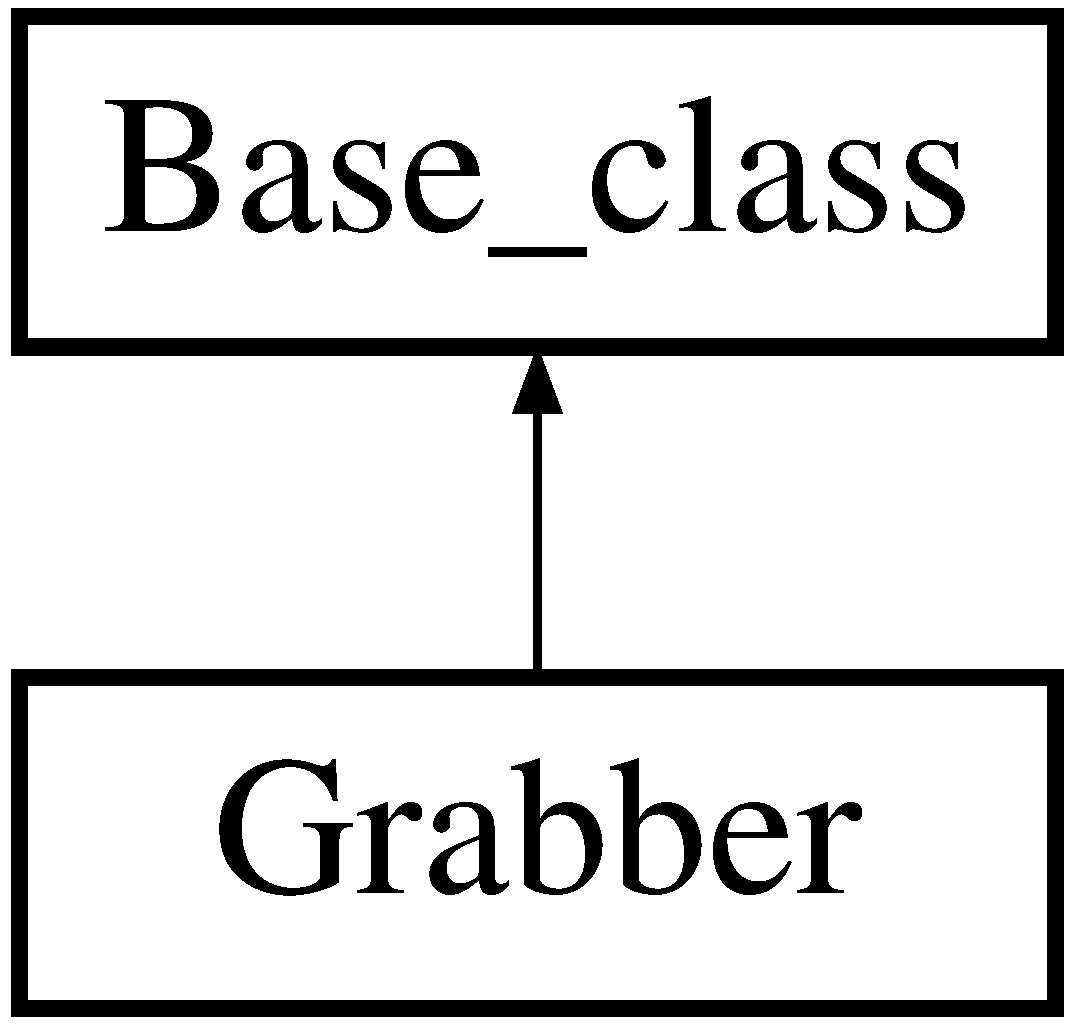
\includegraphics[height=2.000000cm]{classGrabber}
\end{center}
\end{figure}
\subsection*{Public Member Functions}
\begin{DoxyCompactItemize}
\item 
\mbox{\Hypertarget{classGrabber_a0f7dd26f3bf460ee2ac6aa31be2b69bd}\label{classGrabber_a0f7dd26f3bf460ee2ac6aa31be2b69bd}} 
virtual void {\bfseries load\+Params} () override
\item 
\mbox{\Hypertarget{classGrabber_ac37592916381aef27aecccef5a9d25aa}\label{classGrabber_ac37592916381aef27aecccef5a9d25aa}} 
virtual void {\bfseries spin\+Thread\+Front} () override
\item 
\mbox{\Hypertarget{classGrabber_a04796f63552146599ed5247bf65efe9d}\label{classGrabber_a04796f63552146599ed5247bf65efe9d}} 
virtual void {\bfseries spin\+Thread\+Bottom} () override
\end{DoxyCompactItemize}
\subsection*{Additional Inherited Members}


The documentation for this class was generated from the following files\+:\begin{DoxyCompactItemize}
\item 
vision\+\_\+layer/vision\+\_\+tasks/include/grabber.\+h\item 
vision\+\_\+layer/vision\+\_\+tasks/src/grabber.\+cpp\end{DoxyCompactItemize}

\hypertarget{classcolor__correction_1_1gray__edge}{}\section{color\+\_\+correction\+:\+:gray\+\_\+edge Class Reference}
\label{classcolor__correction_1_1gray__edge}\index{color\+\_\+correction\+::gray\+\_\+edge@{color\+\_\+correction\+::gray\+\_\+edge}}
\subsection*{Public Member Functions}
\begin{DoxyCompactItemize}
\item 
Mat \hyperlink{classcolor__correction_1_1gray__edge_a7a8b5fbda7e19f8e48b1ba299e630c3c}{run} (Mat, int p, int m)
\end{DoxyCompactItemize}


\subsection{Member Function Documentation}
\mbox{\Hypertarget{classcolor__correction_1_1gray__edge_a7a8b5fbda7e19f8e48b1ba299e630c3c}\label{classcolor__correction_1_1gray__edge_a7a8b5fbda7e19f8e48b1ba299e630c3c}} 
\index{color\+\_\+correction\+::gray\+\_\+edge@{color\+\_\+correction\+::gray\+\_\+edge}!run@{run}}
\index{run@{run}!color\+\_\+correction\+::gray\+\_\+edge@{color\+\_\+correction\+::gray\+\_\+edge}}
\subsubsection{\texorpdfstring{run()}{run()}}
{\footnotesize\ttfamily Mat color\+\_\+correction\+::gray\+\_\+edge\+::run (\begin{DoxyParamCaption}\item[{Mat}]{src1,  }\item[{int}]{p,  }\item[{int}]{m }\end{DoxyParamCaption})}

this is a main function to call to perform color correction using gray edge algorithm in R\+GB color space 

The documentation for this class was generated from the following files\+:\begin{DoxyCompactItemize}
\item 
vision\+\_\+layer/vision\+\_\+fusion/include/fusion/color\+\_\+constancy.\+hpp\item 
vision\+\_\+layer/vision\+\_\+fusion/src/color\+\_\+constancy.\+cpp\end{DoxyCompactItemize}

\hypertarget{classcolor__correction_1_1gray__world}{}\section{color\+\_\+correction\+:\+:gray\+\_\+world Class Reference}
\label{classcolor__correction_1_1gray__world}\index{color\+\_\+correction\+::gray\+\_\+world@{color\+\_\+correction\+::gray\+\_\+world}}


{\ttfamily \#include $<$color\+\_\+constancy.\+hpp$>$}

\subsection*{Public Member Functions}
\begin{DoxyCompactItemize}
\item 
void \hyperlink{classcolor__correction_1_1gray__world_a5d5afd72d6d11a1ea1e396b9a71da767}{process} (Mat src1, int p, float $\ast$ml, float $\ast$ma, float $\ast$mb)
\item 
void \hyperlink{classcolor__correction_1_1gray__world_a4a0d5ba6b9e4ae8d15a664f6e60b4a24}{process} (Mat src1, float $\ast$ml, float $\ast$ma, float $\ast$mb, int p, int m)
\item 
Mat \hyperlink{classcolor__correction_1_1gray__world_afe9a7e290fa94f8b0c5d67e88b4f206e}{run2} (Mat, int p, int m)
\item 
Mat \hyperlink{classcolor__correction_1_1gray__world_a5d522f9b4cbc22b417463e8542164364}{run1} (Mat, int p)
\end{DoxyCompactItemize}


\subsection{Detailed Description}
class containing methods to perform gray world and shades of gray color correction in R\+GB and Lab Color space 

\subsection{Member Function Documentation}
\mbox{\Hypertarget{classcolor__correction_1_1gray__world_a5d5afd72d6d11a1ea1e396b9a71da767}\label{classcolor__correction_1_1gray__world_a5d5afd72d6d11a1ea1e396b9a71da767}} 
\index{color\+\_\+correction\+::gray\+\_\+world@{color\+\_\+correction\+::gray\+\_\+world}!process@{process}}
\index{process@{process}!color\+\_\+correction\+::gray\+\_\+world@{color\+\_\+correction\+::gray\+\_\+world}}
\subsubsection{\texorpdfstring{process()}{process()}\hspace{0.1cm}{\footnotesize\ttfamily [1/2]}}
{\footnotesize\ttfamily void color\+\_\+correction\+::gray\+\_\+world\+::process (\begin{DoxyParamCaption}\item[{Mat}]{src1,  }\item[{int}]{p,  }\item[{float $\ast$}]{ml,  }\item[{float $\ast$}]{ma,  }\item[{float $\ast$}]{mb }\end{DoxyParamCaption})}

The method to compute the estimate of illumination vector. Inputs are image and norm and outputs are ml, ma, mb the estimate of illumination vector/scaling factors \mbox{\Hypertarget{classcolor__correction_1_1gray__world_a4a0d5ba6b9e4ae8d15a664f6e60b4a24}\label{classcolor__correction_1_1gray__world_a4a0d5ba6b9e4ae8d15a664f6e60b4a24}} 
\index{color\+\_\+correction\+::gray\+\_\+world@{color\+\_\+correction\+::gray\+\_\+world}!process@{process}}
\index{process@{process}!color\+\_\+correction\+::gray\+\_\+world@{color\+\_\+correction\+::gray\+\_\+world}}
\subsubsection{\texorpdfstring{process()}{process()}\hspace{0.1cm}{\footnotesize\ttfamily [2/2]}}
{\footnotesize\ttfamily void color\+\_\+correction\+::gray\+\_\+world\+::process (\begin{DoxyParamCaption}\item[{Mat}]{src1,  }\item[{float $\ast$}]{ml,  }\item[{float $\ast$}]{ma,  }\item[{float $\ast$}]{mb,  }\item[{int}]{p,  }\item[{int}]{m }\end{DoxyParamCaption})}

function to estimate the illumination vector or scaling factor for R\+GB color space computation inputs are the sourc image, minkownski norm factor (p), and three normalization defined by (m = 0, 1, 2) the outputs are the factor ml,ma,mb for each of the color channel \mbox{\Hypertarget{classcolor__correction_1_1gray__world_a5d522f9b4cbc22b417463e8542164364}\label{classcolor__correction_1_1gray__world_a5d522f9b4cbc22b417463e8542164364}} 
\index{color\+\_\+correction\+::gray\+\_\+world@{color\+\_\+correction\+::gray\+\_\+world}!run1@{run1}}
\index{run1@{run1}!color\+\_\+correction\+::gray\+\_\+world@{color\+\_\+correction\+::gray\+\_\+world}}
\subsubsection{\texorpdfstring{run1()}{run1()}}
{\footnotesize\ttfamily Mat color\+\_\+correction\+::gray\+\_\+world\+::run1 (\begin{DoxyParamCaption}\item[{Mat}]{src,  }\item[{int}]{p }\end{DoxyParamCaption})}

This is the main method which to call for color correction in Lab Color space.\+This performs basic pre-\/processing and calls the gray world function \mbox{\Hypertarget{classcolor__correction_1_1gray__world_afe9a7e290fa94f8b0c5d67e88b4f206e}\label{classcolor__correction_1_1gray__world_afe9a7e290fa94f8b0c5d67e88b4f206e}} 
\index{color\+\_\+correction\+::gray\+\_\+world@{color\+\_\+correction\+::gray\+\_\+world}!run2@{run2}}
\index{run2@{run2}!color\+\_\+correction\+::gray\+\_\+world@{color\+\_\+correction\+::gray\+\_\+world}}
\subsubsection{\texorpdfstring{run2()}{run2()}}
{\footnotesize\ttfamily Mat color\+\_\+correction\+::gray\+\_\+world\+::run2 (\begin{DoxyParamCaption}\item[{Mat}]{src,  }\item[{int}]{p,  }\item[{int}]{m }\end{DoxyParamCaption})}

this is a main function to call to perform color correction in R\+GB color space 

The documentation for this class was generated from the following files\+:\begin{DoxyCompactItemize}
\item 
vision\+\_\+layer/vision\+\_\+fusion/include/fusion/color\+\_\+constancy.\+hpp\item 
vision\+\_\+layer/vision\+\_\+fusion/src/color\+\_\+constancy.\+cpp\end{DoxyCompactItemize}

\hypertarget{classuuv__trajectory__generator_1_1path__generator_1_1helical__segment_1_1HelicalSegment}{}\doxysection{uuv\+\_\+trajectory\+\_\+generator.\+path\+\_\+generator.\+helical\+\_\+segment.\+Helical\+Segment Class Reference}
\label{classuuv__trajectory__generator_1_1path__generator_1_1helical__segment_1_1HelicalSegment}\index{uuv\_trajectory\_generator.path\_generator.helical\_segment.HelicalSegment@{uuv\_trajectory\_generator.path\_generator.helical\_segment.HelicalSegment}}
Inheritance diagram for uuv\+\_\+trajectory\+\_\+generator.\+path\+\_\+generator.\+helical\+\_\+segment.\+Helical\+Segment\+:\begin{figure}[H]
\begin{center}
\leavevmode
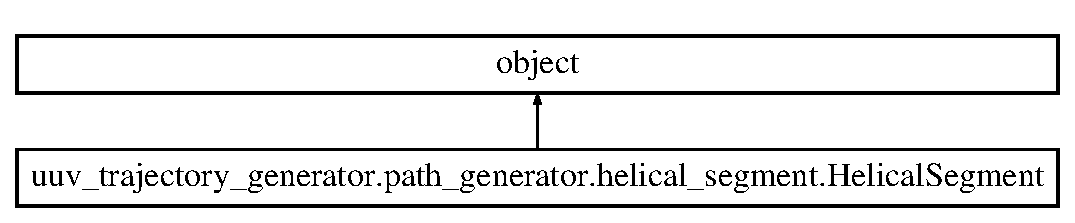
\includegraphics[height=2.000000cm]{classuuv__trajectory__generator_1_1path__generator_1_1helical__segment_1_1HelicalSegment}
\end{center}
\end{figure}
\doxysubsection*{Public Member Functions}
\begin{DoxyCompactItemize}
\item 
\mbox{\Hypertarget{classuuv__trajectory__generator_1_1path__generator_1_1helical__segment_1_1HelicalSegment_a24cd1792f5247ff725fed130c0c36d43}\label{classuuv__trajectory__generator_1_1path__generator_1_1helical__segment_1_1HelicalSegment_a24cd1792f5247ff725fed130c0c36d43}} 
def {\bfseries \+\_\+\+\_\+init\+\_\+\+\_\+} (self, center, radius, n\+\_\+turns, delta\+\_\+z, angle\+\_\+offset, is\+\_\+clockwise=True)
\item 
\mbox{\Hypertarget{classuuv__trajectory__generator_1_1path__generator_1_1helical__segment_1_1HelicalSegment_a629cb0cdbe5d5d7c91c2198d0b024084}\label{classuuv__trajectory__generator_1_1path__generator_1_1helical__segment_1_1HelicalSegment_a629cb0cdbe5d5d7c91c2198d0b024084}} 
def {\bfseries get\+\_\+length} (self)
\item 
\mbox{\Hypertarget{classuuv__trajectory__generator_1_1path__generator_1_1helical__segment_1_1HelicalSegment_acff99fcfcb2246fe7ed422b91186b98e}\label{classuuv__trajectory__generator_1_1path__generator_1_1helical__segment_1_1HelicalSegment_acff99fcfcb2246fe7ed422b91186b98e}} 
def {\bfseries get\+\_\+pitch} (self)
\item 
\mbox{\Hypertarget{classuuv__trajectory__generator_1_1path__generator_1_1helical__segment_1_1HelicalSegment_a03b024443ace910883c336bf5c905877}\label{classuuv__trajectory__generator_1_1path__generator_1_1helical__segment_1_1HelicalSegment_a03b024443ace910883c336bf5c905877}} 
def {\bfseries interpolate} (self, u)
\end{DoxyCompactItemize}


The documentation for this class was generated from the following file\+:\begin{DoxyCompactItemize}
\item 
control\+\_\+layer/uuv\+\_\+trajectory\+\_\+control/src/uuv\+\_\+trajectory\+\_\+generator/path\+\_\+generator/helical\+\_\+segment.\+py\end{DoxyCompactItemize}

\hypertarget{classmaster__layer_1_1state__mach_1_1IdentifyTarget}{}\section{master\+\_\+layer.\+state\+\_\+mach.\+Identify\+Target Class Reference}
\label{classmaster__layer_1_1state__mach_1_1IdentifyTarget}\index{master\+\_\+layer.\+state\+\_\+mach.\+Identify\+Target@{master\+\_\+layer.\+state\+\_\+mach.\+Identify\+Target}}
Inheritance diagram for master\+\_\+layer.\+state\+\_\+mach.\+Identify\+Target\+:\begin{figure}[H]
\begin{center}
\leavevmode
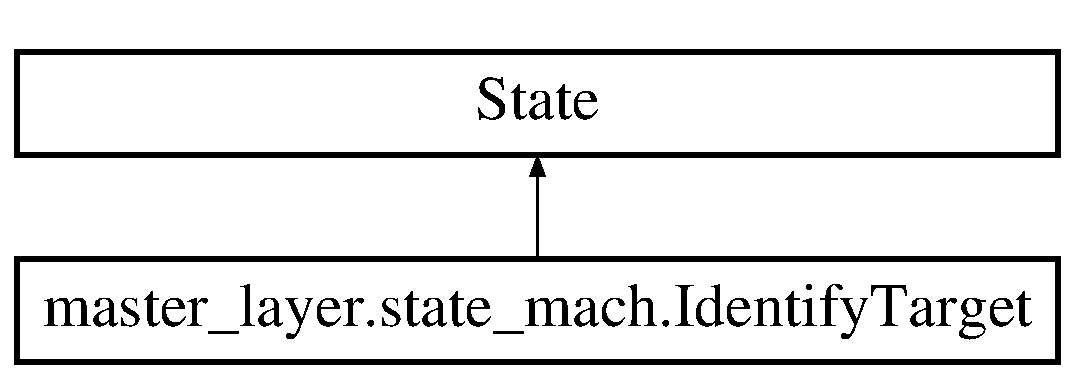
\includegraphics[height=2.000000cm]{classmaster__layer_1_1state__mach_1_1IdentifyTarget}
\end{center}
\end{figure}
\subsection*{Public Member Functions}
\begin{DoxyCompactItemize}
\item 
\mbox{\Hypertarget{classmaster__layer_1_1state__mach_1_1IdentifyTarget_ac7a4630888de1c173fc6188ad61a237d}\label{classmaster__layer_1_1state__mach_1_1IdentifyTarget_ac7a4630888de1c173fc6188ad61a237d}} 
def {\bfseries \+\_\+\+\_\+init\+\_\+\+\_\+} (self)
\end{DoxyCompactItemize}


The documentation for this class was generated from the following file\+:\begin{DoxyCompactItemize}
\item 
master\+\_\+layer/src/master\+\_\+layer/state\+\_\+mach.\+py\end{DoxyCompactItemize}

\hypertarget{classmaster__layer_1_1state__mach__gate__torpedo_1_1IdentifyTarget}{}\doxysection{master\+\_\+layer.\+state\+\_\+mach\+\_\+gate\+\_\+torpedo.\+Identify\+Target Class Reference}
\label{classmaster__layer_1_1state__mach__gate__torpedo_1_1IdentifyTarget}\index{master\_layer.state\_mach\_gate\_torpedo.IdentifyTarget@{master\_layer.state\_mach\_gate\_torpedo.IdentifyTarget}}
Inheritance diagram for master\+\_\+layer.\+state\+\_\+mach\+\_\+gate\+\_\+torpedo.\+Identify\+Target\+:\begin{figure}[H]
\begin{center}
\leavevmode
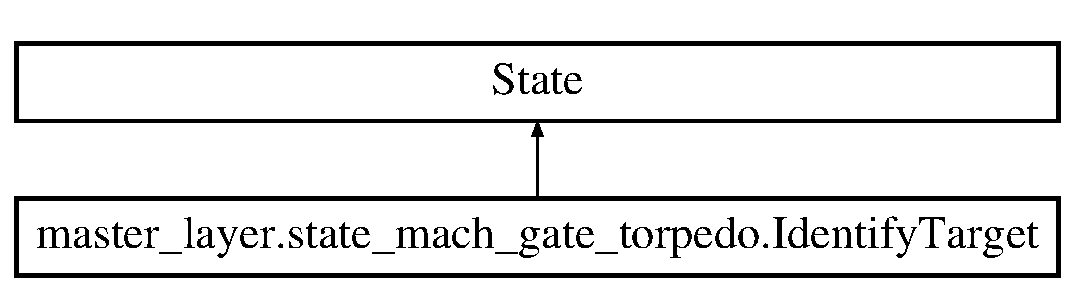
\includegraphics[height=2.000000cm]{classmaster__layer_1_1state__mach__gate__torpedo_1_1IdentifyTarget}
\end{center}
\end{figure}
\doxysubsection*{Public Member Functions}
\begin{DoxyCompactItemize}
\item 
\mbox{\Hypertarget{classmaster__layer_1_1state__mach__gate__torpedo_1_1IdentifyTarget_a430f7d239c95a4a1a7f6d07204abeed9}\label{classmaster__layer_1_1state__mach__gate__torpedo_1_1IdentifyTarget_a430f7d239c95a4a1a7f6d07204abeed9}} 
def {\bfseries \+\_\+\+\_\+init\+\_\+\+\_\+} (self)
\end{DoxyCompactItemize}


The documentation for this class was generated from the following file\+:\begin{DoxyCompactItemize}
\item 
master\+\_\+layer/src/master\+\_\+layer/state\+\_\+mach\+\_\+gate\+\_\+torpedo.\+py\end{DoxyCompactItemize}

\hypertarget{classimage__undistort_1_1ImageUndistort}{}\doxysection{image\+\_\+undistort\+::Image\+Undistort Class Reference}
\label{classimage__undistort_1_1ImageUndistort}\index{image\_undistort::ImageUndistort@{image\_undistort::ImageUndistort}}
\doxysubsection*{Public Member Functions}
\begin{DoxyCompactItemize}
\item 
\mbox{\Hypertarget{classimage__undistort_1_1ImageUndistort_ab3b6622d4eaee133af34a4b786cccc38}\label{classimage__undistort_1_1ImageUndistort_ab3b6622d4eaee133af34a4b786cccc38}} 
{\bfseries Image\+Undistort} (const ros\+::\+Node\+Handle \&nh\+\_\+, const ros\+::\+Node\+Handle \&nh\+\_\+private\+\_\+)
\end{DoxyCompactItemize}


The documentation for this class was generated from the following files\+:\begin{DoxyCompactItemize}
\item 
vision\+\_\+layer/image\+\_\+undistort/include/image\+\_\+undistort/image\+\_\+undistort.\+h\item 
vision\+\_\+layer/image\+\_\+undistort/src/image\+\_\+undistort.\+cpp\end{DoxyCompactItemize}

\hypertarget{classimage__undistort_1_1ImageUndistortNodelet}{}\doxysection{image\+\_\+undistort\+::Image\+Undistort\+Nodelet Class Reference}
\label{classimage__undistort_1_1ImageUndistortNodelet}\index{image\_undistort::ImageUndistortNodelet@{image\_undistort::ImageUndistortNodelet}}
Inheritance diagram for image\+\_\+undistort\+::Image\+Undistort\+Nodelet\+:\begin{figure}[H]
\begin{center}
\leavevmode
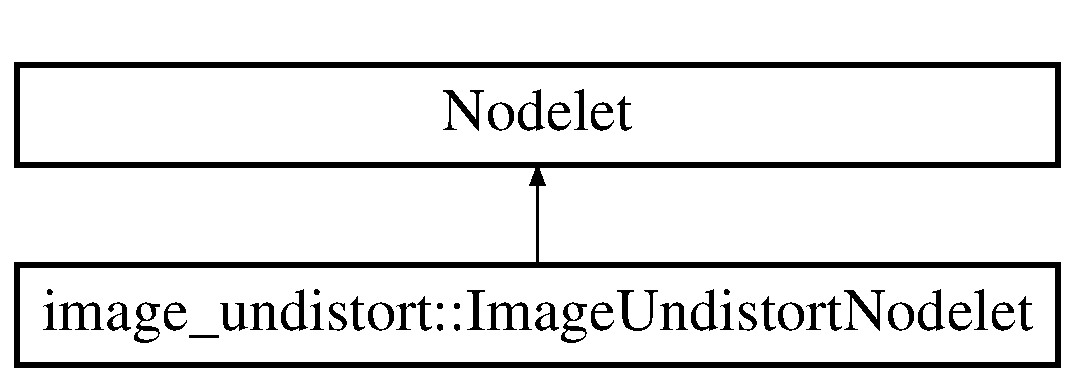
\includegraphics[height=2.000000cm]{classimage__undistort_1_1ImageUndistortNodelet}
\end{center}
\end{figure}


The documentation for this class was generated from the following file\+:\begin{DoxyCompactItemize}
\item 
vision\+\_\+layer/image\+\_\+undistort/src/nodelets/image\+\_\+undistort\+\_\+nodelet.\+cpp\end{DoxyCompactItemize}

\hypertarget{classnavigation_1_1IMUData}{}\doxysection{navigation\+::I\+M\+U\+Data Class Reference}
\label{classnavigation_1_1IMUData}\index{navigation::IMUData@{navigation::IMUData}}
Inheritance diagram for navigation\+::I\+M\+U\+Data\+:\begin{figure}[H]
\begin{center}
\leavevmode
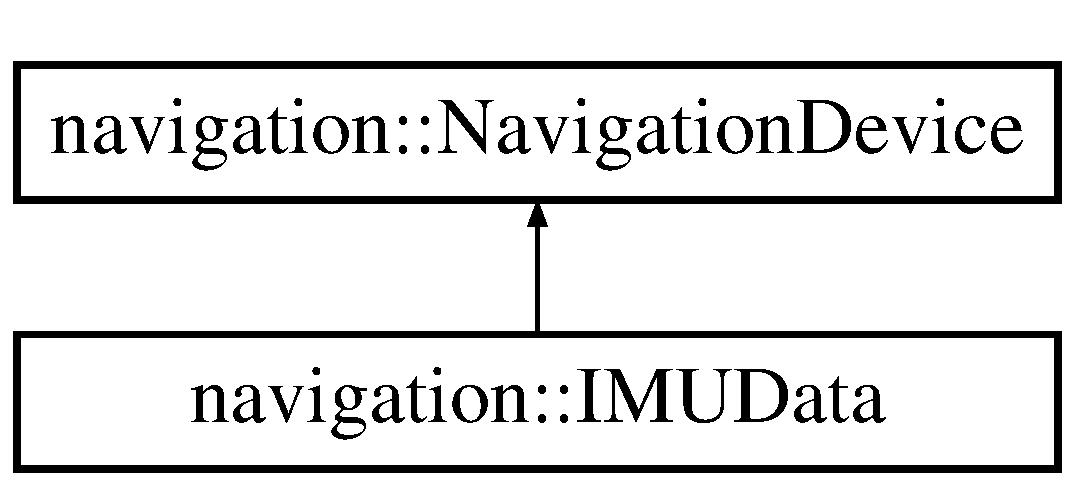
\includegraphics[height=2.000000cm]{classnavigation_1_1IMUData}
\end{center}
\end{figure}
\doxysubsection*{Public Member Functions}
\begin{DoxyCompactItemize}
\item 
\mbox{\Hypertarget{classnavigation_1_1IMUData_a56f1c6d51df94b59ff64c1d0521f10df}\label{classnavigation_1_1IMUData_a56f1c6d51df94b59ff64c1d0521f10df}} 
void {\bfseries I\+M\+U\+Msg\+Callback} (sensor\+\_\+msgs\+::\+Imu msg)
\item 
\mbox{\Hypertarget{classnavigation_1_1IMUData_a3aa9b882f36194d91420e3515d6ae2b1}\label{classnavigation_1_1IMUData_a3aa9b882f36194d91420e3515d6ae2b1}} 
Eigen\+::\+Quaterniond {\bfseries Get\+Quaternion} ()
\item 
\mbox{\Hypertarget{classnavigation_1_1IMUData_a2e0cf1bcc3e0123beb9f33bafee823bc}\label{classnavigation_1_1IMUData_a2e0cf1bcc3e0123beb9f33bafee823bc}} 
Eigen\+::\+Vector3d {\bfseries Get\+Orientation} ()
\item 
\mbox{\Hypertarget{classnavigation_1_1IMUData_aca709ec30e406aba9a4270b72784cb65}\label{classnavigation_1_1IMUData_aca709ec30e406aba9a4270b72784cb65}} 
Eigen\+::\+Vector3d {\bfseries Get\+Angular\+Velocity} ()
\end{DoxyCompactItemize}
\doxysubsection*{Public Attributes}
\begin{DoxyCompactItemize}
\item 
\mbox{\Hypertarget{classnavigation_1_1IMUData_afa6279c235420123416323ced87e7103}\label{classnavigation_1_1IMUData_afa6279c235420123416323ced87e7103}} 
const double {\bfseries R\+A\+D\+\_\+\+T\+O\+\_\+\+D\+E\+G\+R\+EE} = 180.\+0f / M\+\_\+\+PI
\end{DoxyCompactItemize}


The documentation for this class was generated from the following files\+:\begin{DoxyCompactItemize}
\item 
navigation\+\_\+layer/odom\+\_\+dvl\+\_\+imu/include/imu\+\_\+data.\+h\item 
navigation\+\_\+layer/odom\+\_\+dvl\+\_\+imu/src/imu\+\_\+data.\+cpp\end{DoxyCompactItemize}

\hypertarget{classimage__undistort_1_1InputCameraParameters}{}\doxysection{image\+\_\+undistort\+::Input\+Camera\+Parameters Class Reference}
\label{classimage__undistort_1_1InputCameraParameters}\index{image\_undistort::InputCameraParameters@{image\_undistort::InputCameraParameters}}
Inheritance diagram for image\+\_\+undistort\+::Input\+Camera\+Parameters\+:\begin{figure}[H]
\begin{center}
\leavevmode
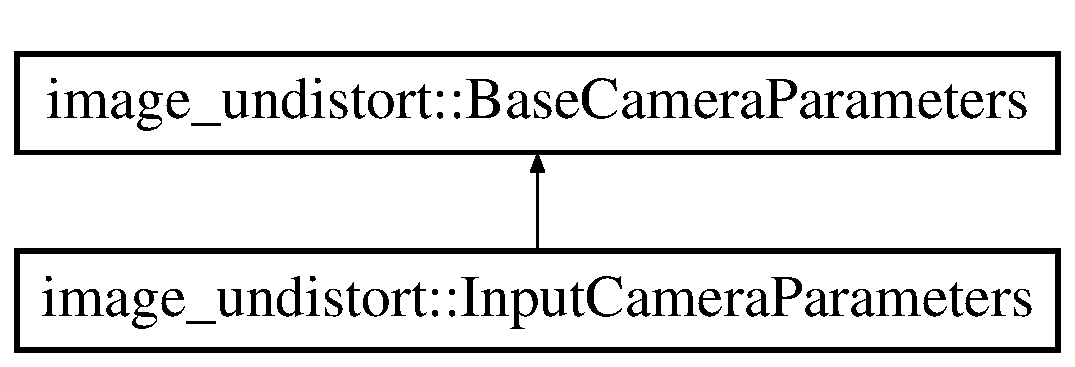
\includegraphics[height=2.000000cm]{classimage__undistort_1_1InputCameraParameters}
\end{center}
\end{figure}
\doxysubsection*{Public Member Functions}
\begin{DoxyCompactItemize}
\item 
\mbox{\Hypertarget{classimage__undistort_1_1InputCameraParameters_a33bd851feb1a1eb1bd16243f06c200dc}\label{classimage__undistort_1_1InputCameraParameters_a33bd851feb1a1eb1bd16243f06c200dc}} 
{\bfseries Input\+Camera\+Parameters} (const ros\+::\+Node\+Handle \&nh, const std\+::string \&camera\+\_\+namespace, const bool invert\+\_\+T=false)
\item 
\mbox{\Hypertarget{classimage__undistort_1_1InputCameraParameters_a547a641f1838cf2039107f4e2ee12807}\label{classimage__undistort_1_1InputCameraParameters_a547a641f1838cf2039107f4e2ee12807}} 
{\bfseries Input\+Camera\+Parameters} (const sensor\+\_\+msgs\+::\+Camera\+Info \&camera\+\_\+info)
\item 
\mbox{\Hypertarget{classimage__undistort_1_1InputCameraParameters_af6b25a0e4ae5dbe0b1ca2281ad47fc9f}\label{classimage__undistort_1_1InputCameraParameters_af6b25a0e4ae5dbe0b1ca2281ad47fc9f}} 
{\bfseries Input\+Camera\+Parameters} (const cv\+::\+Size \&resolution\+\_\+in, const Eigen\+::\+Matrix$<$ double, 4, 4 $>$ \&T\+\_\+in, const Eigen\+::\+Matrix$<$ double, 3, 3 $>$ \&K\+\_\+in, const std\+::vector$<$ double $>$ \&D\+\_\+in, const Distortion\+Model \&distortion\+\_\+model)
\item 
\mbox{\Hypertarget{classimage__undistort_1_1InputCameraParameters_a04944a2e3227ca7c1c2fd45f24fca350}\label{classimage__undistort_1_1InputCameraParameters_a04944a2e3227ca7c1c2fd45f24fca350}} 
const std\+::vector$<$ double $>$ \& {\bfseries D} () const
\item 
\mbox{\Hypertarget{classimage__undistort_1_1InputCameraParameters_ac5ea174097c615b5b49ffa6df47d7c4b}\label{classimage__undistort_1_1InputCameraParameters_ac5ea174097c615b5b49ffa6df47d7c4b}} 
const Distortion\+Model \& {\bfseries distortion\+Model} () const
\item 
\mbox{\Hypertarget{classimage__undistort_1_1InputCameraParameters_a5c9c728eb090a6a7836434be0a45f612}\label{classimage__undistort_1_1InputCameraParameters_a5c9c728eb090a6a7836434be0a45f612}} 
bool {\bfseries operator==} (const \mbox{\hyperlink{classimage__undistort_1_1InputCameraParameters}{Input\+Camera\+Parameters}} \&B) const
\item 
\mbox{\Hypertarget{classimage__undistort_1_1InputCameraParameters_ae89f73ebec8690dfff2061c04131ad02}\label{classimage__undistort_1_1InputCameraParameters_ae89f73ebec8690dfff2061c04131ad02}} 
bool {\bfseries operator!=} (const \mbox{\hyperlink{classimage__undistort_1_1InputCameraParameters}{Input\+Camera\+Parameters}} \&B) const
\end{DoxyCompactItemize}


The documentation for this class was generated from the following files\+:\begin{DoxyCompactItemize}
\item 
vision\+\_\+layer/image\+\_\+undistort/include/image\+\_\+undistort/camera\+\_\+parameters.\+h\item 
vision\+\_\+layer/image\+\_\+undistort/src/camera\+\_\+parameters.\+cpp\end{DoxyCompactItemize}

\hypertarget{classLaplacianBlending}{}\doxysection{Laplacian\+Blending Class Reference}
\label{classLaplacianBlending}\index{LaplacianBlending@{LaplacianBlending}}
\doxysubsection*{Public Member Functions}
\begin{DoxyCompactItemize}
\item 
\mbox{\Hypertarget{classLaplacianBlending_a49d7f455a4c06eee3b8a0f328f6d7030}\label{classLaplacianBlending_a49d7f455a4c06eee3b8a0f328f6d7030}} 
{\bfseries Laplacian\+Blending} (const Mat\+\_\+$<$ Vec3f $>$ \&\+\_\+left, const Mat\+\_\+$<$ Vec3f $>$ \&\+\_\+right, const Mat\+\_\+$<$ float $>$ \&\+\_\+left\+Mask, const Mat\+\_\+$<$ float $>$ \&\+\_\+right\+Mask, int \+\_\+levels)
\item 
\mbox{\Hypertarget{classLaplacianBlending_aa700402157dc7ed848724f6edd0b5d4e}\label{classLaplacianBlending_aa700402157dc7ed848724f6edd0b5d4e}} 
Mat\+\_\+$<$ Vec3f $>$ {\bfseries blend} ()
\end{DoxyCompactItemize}


The documentation for this class was generated from the following files\+:\begin{DoxyCompactItemize}
\item 
vision\+\_\+layer/vision\+\_\+fusion/include/fusion/laplacian\+Blend.\+hpp\item 
vision\+\_\+layer/vision\+\_\+fusion/src/laplacian\+Blend.\+cpp\end{DoxyCompactItemize}

\hypertarget{classLine}{}\doxysection{Line Class Reference}
\label{classLine}\index{Line@{Line}}
Inheritance diagram for Line\+:\begin{figure}[H]
\begin{center}
\leavevmode
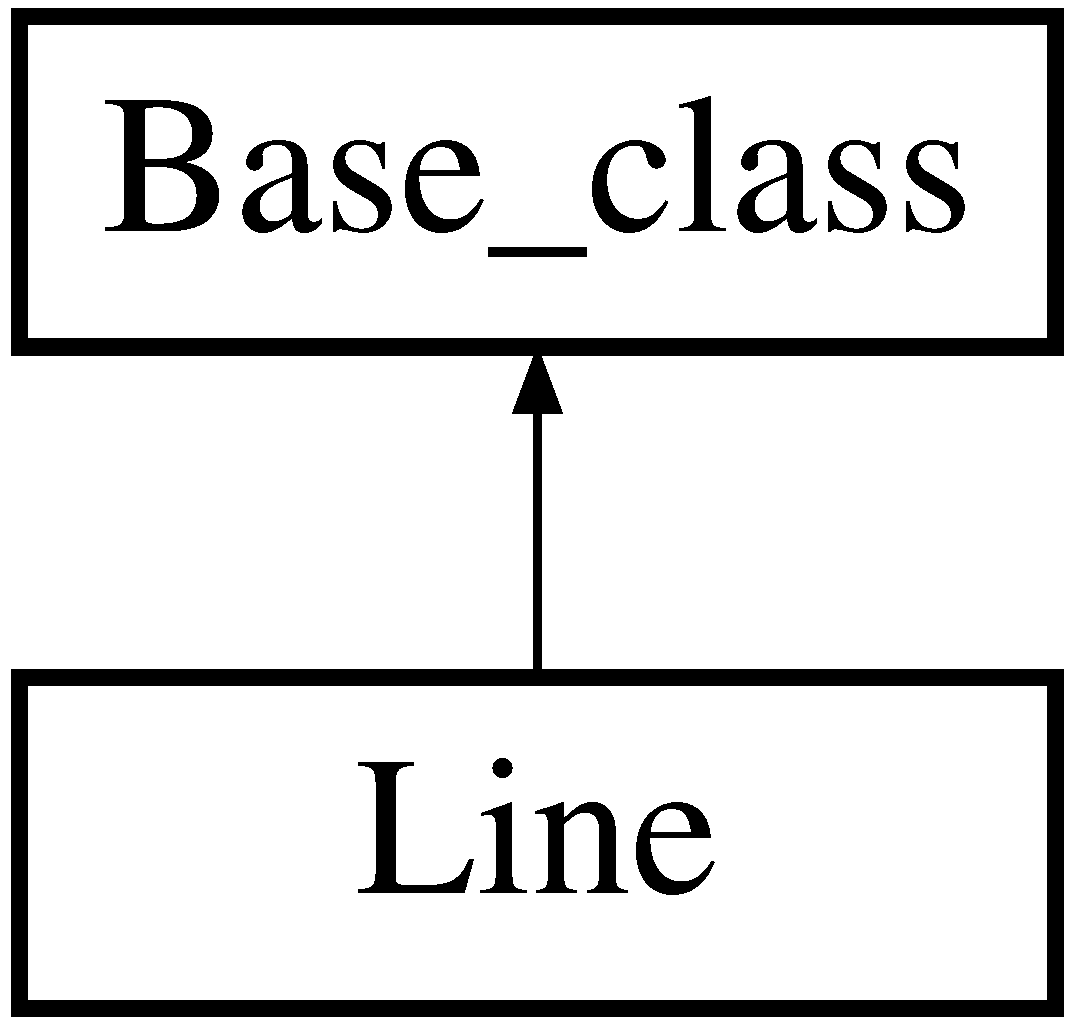
\includegraphics[height=2.000000cm]{classLine}
\end{center}
\end{figure}
\doxysubsection*{Public Member Functions}
\begin{DoxyCompactItemize}
\item 
\mbox{\Hypertarget{classLine_ae0baab0d7e417e7debb04ca7f1f3d0bd}\label{classLine_ae0baab0d7e417e7debb04ca7f1f3d0bd}} 
void {\bfseries spin\+Thread\+Bottom} ()
\end{DoxyCompactItemize}
\doxysubsection*{Protected Member Functions}
\begin{DoxyCompactItemize}
\item 
\mbox{\Hypertarget{classLine_adaec4c36ed87a85ef20dedae0dc64e3a}\label{classLine_adaec4c36ed87a85ef20dedae0dc64e3a}} 
void {\bfseries callback} (vision\+\_\+tasks\+::line\+Range\+Config \&config, double level)
\item 
\mbox{\Hypertarget{classLine_a4fd089a81700282003dc3b4f3a9c6ac4}\label{classLine_a4fd089a81700282003dc3b4f3a9c6ac4}} 
void {\bfseries image\+Callback} (const sensor\+\_\+msgs\+::\+Image\+::\+Const\+Ptr \&msg)
\item 
\mbox{\Hypertarget{classLine_a23aae96dede860bd33b5e57221701bfa}\label{classLine_a23aae96dede860bd33b5e57221701bfa}} 
double {\bfseries compute\+Mean} (std\+::vector$<$ double $>$ \&new\+Angles)
\end{DoxyCompactItemize}
\doxysubsection*{Protected Attributes}
\begin{DoxyCompactItemize}
\item 
\mbox{\Hypertarget{classLine_a7baec58f43b0596a630e086591e4e072}\label{classLine_a7baec58f43b0596a630e086591e4e072}} 
image\+\_\+transport\+::\+Subscriber {\bfseries image\+\_\+raw\+\_\+sub}
\item 
\mbox{\Hypertarget{classLine_ae41bf70d070b2abcca4e8d289a86b85a}\label{classLine_ae41bf70d070b2abcca4e8d289a86b85a}} 
ros\+::\+Publisher {\bfseries detection\+\_\+pub}
\item 
\mbox{\Hypertarget{classLine_adecc2f839c1de6c5e6f5baff29951db9}\label{classLine_adecc2f839c1de6c5e6f5baff29951db9}} 
ros\+::\+Publisher {\bfseries coordinates\+\_\+pub}
\item 
\mbox{\Hypertarget{classLine_a61ee6db6c19464de515c754cf8a99731}\label{classLine_a61ee6db6c19464de515c754cf8a99731}} 
std\+::string {\bfseries camera\+\_\+frame\+\_\+}
\item 
\mbox{\Hypertarget{classLine_a6139a8ba5889f7e4384dddf05b5f83d2}\label{classLine_a6139a8ba5889f7e4384dddf05b5f83d2}} 
bool {\bfseries task\+\_\+done} = false
\item 
\mbox{\Hypertarget{classLine_a6f522c0976cbe9b76bfbe89fa423ce25}\label{classLine_a6f522c0976cbe9b76bfbe89fa423ce25}} 
ros\+::\+Publisher {\bfseries ang\+\_\+pub}
\end{DoxyCompactItemize}
\doxysubsection*{Additional Inherited Members}


The documentation for this class was generated from the following files\+:\begin{DoxyCompactItemize}
\item 
vision\+\_\+layer/vision\+\_\+tasks/include/line.\+h\item 
vision\+\_\+layer/vision\+\_\+tasks/src/line.\+cpp\end{DoxyCompactItemize}

\hypertarget{classuuv__trajectory__generator_1_1path__generator_1_1linear__interpolator_1_1LinearInterpolator}{}\section{uuv\+\_\+trajectory\+\_\+generator.\+path\+\_\+generator.\+linear\+\_\+interpolator.\+Linear\+Interpolator Class Reference}
\label{classuuv__trajectory__generator_1_1path__generator_1_1linear__interpolator_1_1LinearInterpolator}\index{uuv\+\_\+trajectory\+\_\+generator.\+path\+\_\+generator.\+linear\+\_\+interpolator.\+Linear\+Interpolator@{uuv\+\_\+trajectory\+\_\+generator.\+path\+\_\+generator.\+linear\+\_\+interpolator.\+Linear\+Interpolator}}
Inheritance diagram for uuv\+\_\+trajectory\+\_\+generator.\+path\+\_\+generator.\+linear\+\_\+interpolator.\+Linear\+Interpolator\+:\begin{figure}[H]
\begin{center}
\leavevmode
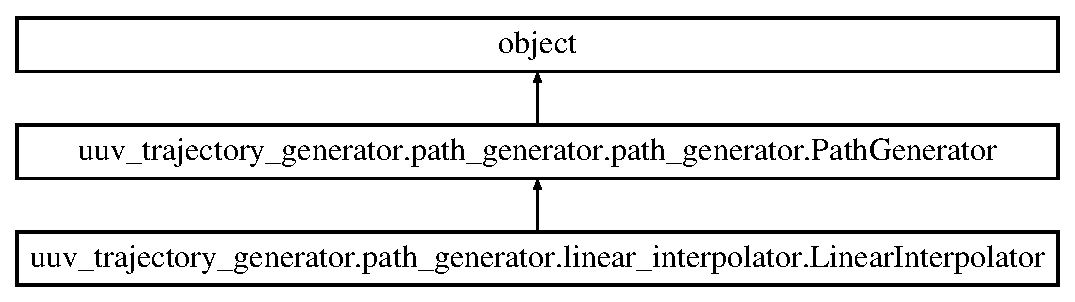
\includegraphics[height=3.000000cm]{classuuv__trajectory__generator_1_1path__generator_1_1linear__interpolator_1_1LinearInterpolator}
\end{center}
\end{figure}
\subsection*{Public Member Functions}
\begin{DoxyCompactItemize}
\item 
\mbox{\Hypertarget{classuuv__trajectory__generator_1_1path__generator_1_1linear__interpolator_1_1LinearInterpolator_a156e00f0c1133260a0c9a3fa417eccfe}\label{classuuv__trajectory__generator_1_1path__generator_1_1linear__interpolator_1_1LinearInterpolator_a156e00f0c1133260a0c9a3fa417eccfe}} 
def {\bfseries \+\_\+\+\_\+init\+\_\+\+\_\+} (self)
\item 
\mbox{\Hypertarget{classuuv__trajectory__generator_1_1path__generator_1_1linear__interpolator_1_1LinearInterpolator_a124d940e6ed64dc12371dd748a1eb1da}\label{classuuv__trajectory__generator_1_1path__generator_1_1linear__interpolator_1_1LinearInterpolator_a124d940e6ed64dc12371dd748a1eb1da}} 
def {\bfseries init\+\_\+interpolator} (self)
\item 
def \hyperlink{classuuv__trajectory__generator_1_1path__generator_1_1linear__interpolator_1_1LinearInterpolator_aaf9e32094bc17645ffa2846aae9e5d79}{set\+\_\+parameters} (self, params)
\item 
\mbox{\Hypertarget{classuuv__trajectory__generator_1_1path__generator_1_1linear__interpolator_1_1LinearInterpolator_a645b70f404c9ef99d21d66946590705d}\label{classuuv__trajectory__generator_1_1path__generator_1_1linear__interpolator_1_1LinearInterpolator_a645b70f404c9ef99d21d66946590705d}} 
def {\bfseries get\+\_\+samples} (self, max\+\_\+time, step=0.\+001)
\item 
\mbox{\Hypertarget{classuuv__trajectory__generator_1_1path__generator_1_1linear__interpolator_1_1LinearInterpolator_a00eb363f3086e4311755d8588f97969f}\label{classuuv__trajectory__generator_1_1path__generator_1_1linear__interpolator_1_1LinearInterpolator_a00eb363f3086e4311755d8588f97969f}} 
def {\bfseries generate\+\_\+pos} (self, s)
\item 
\mbox{\Hypertarget{classuuv__trajectory__generator_1_1path__generator_1_1linear__interpolator_1_1LinearInterpolator_abe3258a0736d19e7bcfb5ff4bb35abc2}\label{classuuv__trajectory__generator_1_1path__generator_1_1linear__interpolator_1_1LinearInterpolator_abe3258a0736d19e7bcfb5ff4bb35abc2}} 
def {\bfseries generate\+\_\+pnt} (self, s, t, args)
\item 
\mbox{\Hypertarget{classuuv__trajectory__generator_1_1path__generator_1_1linear__interpolator_1_1LinearInterpolator_ac3cd4dc5ebcc1fac51eed720dae170d5}\label{classuuv__trajectory__generator_1_1path__generator_1_1linear__interpolator_1_1LinearInterpolator_ac3cd4dc5ebcc1fac51eed720dae170d5}} 
def {\bfseries generate\+\_\+quat} (self, s)
\end{DoxyCompactItemize}
\subsection*{Static Public Attributes}
\begin{DoxyCompactItemize}
\item 
\mbox{\Hypertarget{classuuv__trajectory__generator_1_1path__generator_1_1linear__interpolator_1_1LinearInterpolator_ae99812efadf9ce27863ddd21fce60ba2}\label{classuuv__trajectory__generator_1_1path__generator_1_1linear__interpolator_1_1LinearInterpolator_ae99812efadf9ce27863ddd21fce60ba2}} 
string {\bfseries L\+A\+B\+EL} = \textquotesingle{}linear\textquotesingle{}
\end{DoxyCompactItemize}
\subsection*{Additional Inherited Members}


\subsection{Detailed Description}
\begin{DoxyVerb}Simple linear interpolator
\end{DoxyVerb}
 

\subsection{Member Function Documentation}
\mbox{\Hypertarget{classuuv__trajectory__generator_1_1path__generator_1_1linear__interpolator_1_1LinearInterpolator_aaf9e32094bc17645ffa2846aae9e5d79}\label{classuuv__trajectory__generator_1_1path__generator_1_1linear__interpolator_1_1LinearInterpolator_aaf9e32094bc17645ffa2846aae9e5d79}} 
\index{uuv\+\_\+trajectory\+\_\+generator\+::path\+\_\+generator\+::linear\+\_\+interpolator\+::\+Linear\+Interpolator@{uuv\+\_\+trajectory\+\_\+generator\+::path\+\_\+generator\+::linear\+\_\+interpolator\+::\+Linear\+Interpolator}!set\+\_\+parameters@{set\+\_\+parameters}}
\index{set\+\_\+parameters@{set\+\_\+parameters}!uuv\+\_\+trajectory\+\_\+generator\+::path\+\_\+generator\+::linear\+\_\+interpolator\+::\+Linear\+Interpolator@{uuv\+\_\+trajectory\+\_\+generator\+::path\+\_\+generator\+::linear\+\_\+interpolator\+::\+Linear\+Interpolator}}
\subsubsection{\texorpdfstring{set\+\_\+parameters()}{set\_parameters()}}
{\footnotesize\ttfamily def uuv\+\_\+trajectory\+\_\+generator.\+path\+\_\+generator.\+linear\+\_\+interpolator.\+Linear\+Interpolator.\+set\+\_\+parameters (\begin{DoxyParamCaption}\item[{}]{self,  }\item[{}]{params }\end{DoxyParamCaption})}

\begin{DoxyVerb}Not implemented for this interpolator.\end{DoxyVerb}
 

The documentation for this class was generated from the following file\+:\begin{DoxyCompactItemize}
\item 
control\+\_\+layer/uuv\+\_\+trajectory\+\_\+control/src/uuv\+\_\+trajectory\+\_\+generator/path\+\_\+generator/linear\+\_\+interpolator.\+py\end{DoxyCompactItemize}

\hypertarget{classuuv__trajectory__generator_1_1path__generator_1_1line__segment_1_1LineSegment}{}\section{uuv\+\_\+trajectory\+\_\+generator.\+path\+\_\+generator.\+line\+\_\+segment.\+Line\+Segment Class Reference}
\label{classuuv__trajectory__generator_1_1path__generator_1_1line__segment_1_1LineSegment}\index{uuv\+\_\+trajectory\+\_\+generator.\+path\+\_\+generator.\+line\+\_\+segment.\+Line\+Segment@{uuv\+\_\+trajectory\+\_\+generator.\+path\+\_\+generator.\+line\+\_\+segment.\+Line\+Segment}}
Inheritance diagram for uuv\+\_\+trajectory\+\_\+generator.\+path\+\_\+generator.\+line\+\_\+segment.\+Line\+Segment\+:\begin{figure}[H]
\begin{center}
\leavevmode
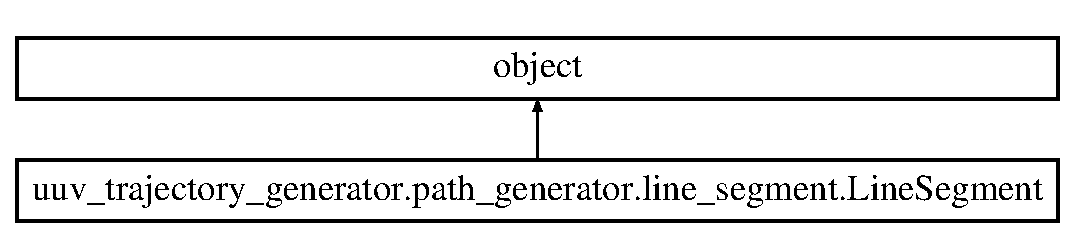
\includegraphics[height=2.000000cm]{classuuv__trajectory__generator_1_1path__generator_1_1line__segment_1_1LineSegment}
\end{center}
\end{figure}
\subsection*{Public Member Functions}
\begin{DoxyCompactItemize}
\item 
\mbox{\Hypertarget{classuuv__trajectory__generator_1_1path__generator_1_1line__segment_1_1LineSegment_acb49e9fa3b6ab890625daa5abe61ef31}\label{classuuv__trajectory__generator_1_1path__generator_1_1line__segment_1_1LineSegment_acb49e9fa3b6ab890625daa5abe61ef31}} 
def {\bfseries \+\_\+\+\_\+init\+\_\+\+\_\+} (self, p\+\_\+init, p\+\_\+target)
\item 
\mbox{\Hypertarget{classuuv__trajectory__generator_1_1path__generator_1_1line__segment_1_1LineSegment_a9aad830ce5fa990021cea72f950ee193}\label{classuuv__trajectory__generator_1_1path__generator_1_1line__segment_1_1LineSegment_a9aad830ce5fa990021cea72f950ee193}} 
def {\bfseries interpolate} (self, u)
\item 
\mbox{\Hypertarget{classuuv__trajectory__generator_1_1path__generator_1_1line__segment_1_1LineSegment_a8efe4da5d86abc6a01df1724b166dffe}\label{classuuv__trajectory__generator_1_1path__generator_1_1line__segment_1_1LineSegment_a8efe4da5d86abc6a01df1724b166dffe}} 
def {\bfseries get\+\_\+derivative} (self, args)
\item 
\mbox{\Hypertarget{classuuv__trajectory__generator_1_1path__generator_1_1line__segment_1_1LineSegment_a7618de32bc394fe55ec18018f51ebb33}\label{classuuv__trajectory__generator_1_1path__generator_1_1line__segment_1_1LineSegment_a7618de32bc394fe55ec18018f51ebb33}} 
def {\bfseries get\+\_\+length} (self)
\item 
\mbox{\Hypertarget{classuuv__trajectory__generator_1_1path__generator_1_1line__segment_1_1LineSegment_a35328684d4961cff4901629475474ba2}\label{classuuv__trajectory__generator_1_1path__generator_1_1line__segment_1_1LineSegment_a35328684d4961cff4901629475474ba2}} 
def {\bfseries get\+\_\+tangent} (self)
\end{DoxyCompactItemize}


The documentation for this class was generated from the following file\+:\begin{DoxyCompactItemize}
\item 
control\+\_\+layer/uuv\+\_\+trajectory\+\_\+control/src/uuv\+\_\+trajectory\+\_\+generator/path\+\_\+generator/line\+\_\+segment.\+py\end{DoxyCompactItemize}

\hypertarget{classmaster__layer_1_1state__mach_1_1LineTask}{}\section{master\+\_\+layer.\+state\+\_\+mach.\+Line\+Task Class Reference}
\label{classmaster__layer_1_1state__mach_1_1LineTask}\index{master\+\_\+layer.\+state\+\_\+mach.\+Line\+Task@{master\+\_\+layer.\+state\+\_\+mach.\+Line\+Task}}
Inheritance diagram for master\+\_\+layer.\+state\+\_\+mach.\+Line\+Task\+:\begin{figure}[H]
\begin{center}
\leavevmode
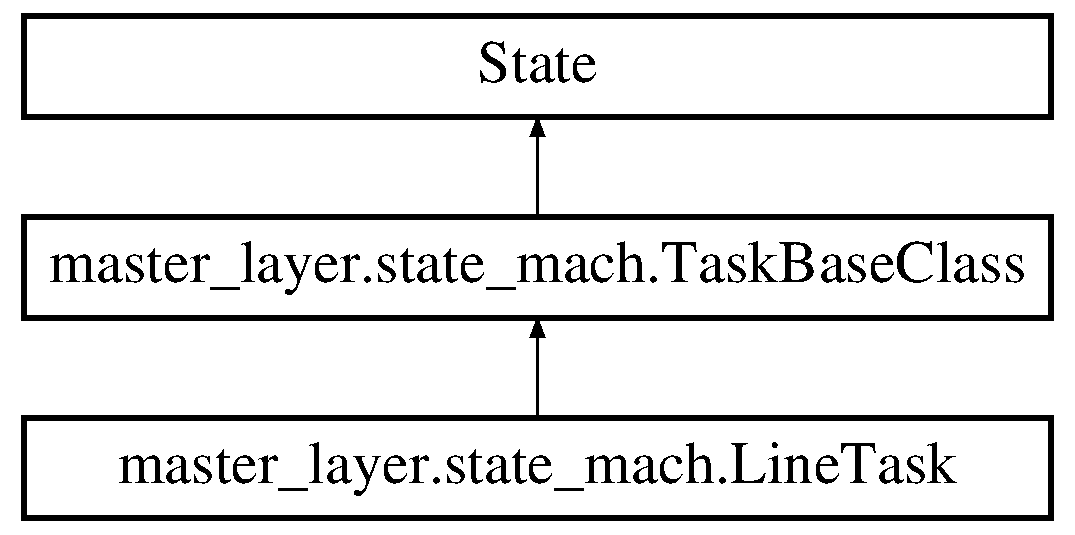
\includegraphics[height=3.000000cm]{classmaster__layer_1_1state__mach_1_1LineTask}
\end{center}
\end{figure}
\subsection*{Public Member Functions}
\begin{DoxyCompactItemize}
\item 
\mbox{\Hypertarget{classmaster__layer_1_1state__mach_1_1LineTask_a29ab835b684e081ac57da871385d5d3c}\label{classmaster__layer_1_1state__mach_1_1LineTask_a29ab835b684e081ac57da871385d5d3c}} 
def {\bfseries \+\_\+\+\_\+init\+\_\+\+\_\+} (self)
\item 
\mbox{\Hypertarget{classmaster__layer_1_1state__mach_1_1LineTask_a13274219ef37814fec9db88097ca612b}\label{classmaster__layer_1_1state__mach_1_1LineTask_a13274219ef37814fec9db88097ca612b}} 
def {\bfseries align} (self)
\item 
\mbox{\Hypertarget{classmaster__layer_1_1state__mach_1_1LineTask_a1ac0acf2d0ec2c8cec80371f644c8d7b}\label{classmaster__layer_1_1state__mach_1_1LineTask_a1ac0acf2d0ec2c8cec80371f644c8d7b}} 
def {\bfseries move\+\_\+forward} (self)
\item 
\mbox{\Hypertarget{classmaster__layer_1_1state__mach_1_1LineTask_a14c494a0b2dbe034ab1e0d9e55e71608}\label{classmaster__layer_1_1state__mach_1_1LineTask_a14c494a0b2dbe034ab1e0d9e55e71608}} 
def {\bfseries execute} (self)
\end{DoxyCompactItemize}


The documentation for this class was generated from the following file\+:\begin{DoxyCompactItemize}
\item 
master\+\_\+layer/src/master\+\_\+layer/state\+\_\+mach.\+py\end{DoxyCompactItemize}

\hypertarget{classmaster__layer_1_1state__mach__gate__torpedo_1_1LineTask}{}\section{master\+\_\+layer.\+state\+\_\+mach\+\_\+gate\+\_\+torpedo.\+Line\+Task Class Reference}
\label{classmaster__layer_1_1state__mach__gate__torpedo_1_1LineTask}\index{master\+\_\+layer.\+state\+\_\+mach\+\_\+gate\+\_\+torpedo.\+Line\+Task@{master\+\_\+layer.\+state\+\_\+mach\+\_\+gate\+\_\+torpedo.\+Line\+Task}}
Inheritance diagram for master\+\_\+layer.\+state\+\_\+mach\+\_\+gate\+\_\+torpedo.\+Line\+Task\+:\begin{figure}[H]
\begin{center}
\leavevmode
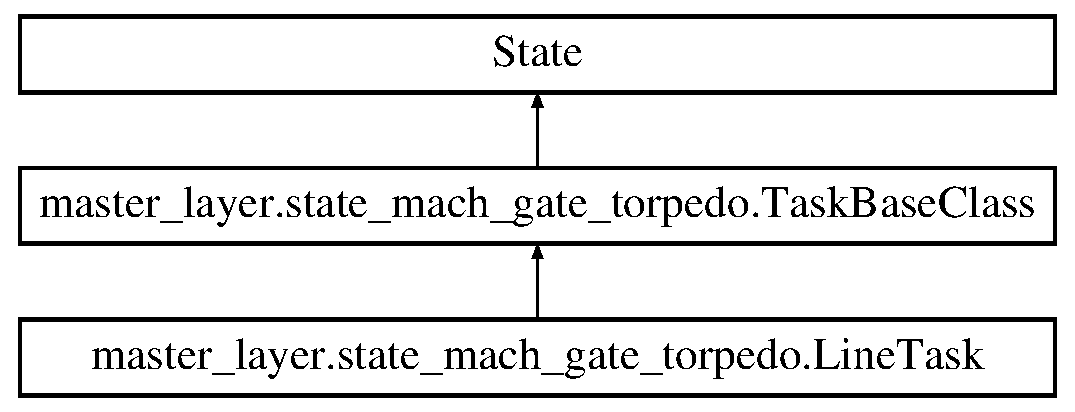
\includegraphics[height=3.000000cm]{classmaster__layer_1_1state__mach__gate__torpedo_1_1LineTask}
\end{center}
\end{figure}
\subsection*{Public Member Functions}
\begin{DoxyCompactItemize}
\item 
\mbox{\Hypertarget{classmaster__layer_1_1state__mach__gate__torpedo_1_1LineTask_a0ae0f1d37820462af30df2f51d2f84db}\label{classmaster__layer_1_1state__mach__gate__torpedo_1_1LineTask_a0ae0f1d37820462af30df2f51d2f84db}} 
def {\bfseries \+\_\+\+\_\+init\+\_\+\+\_\+} (self)
\item 
\mbox{\Hypertarget{classmaster__layer_1_1state__mach__gate__torpedo_1_1LineTask_aad09c73e87d18f78195e75099450e07a}\label{classmaster__layer_1_1state__mach__gate__torpedo_1_1LineTask_aad09c73e87d18f78195e75099450e07a}} 
def {\bfseries align} (self)
\item 
\mbox{\Hypertarget{classmaster__layer_1_1state__mach__gate__torpedo_1_1LineTask_a7bc184fa92c7ef53995eba754bb26d23}\label{classmaster__layer_1_1state__mach__gate__torpedo_1_1LineTask_a7bc184fa92c7ef53995eba754bb26d23}} 
def {\bfseries move\+\_\+forward} (self)
\item 
\mbox{\Hypertarget{classmaster__layer_1_1state__mach__gate__torpedo_1_1LineTask_ac83da84e3d44b5be3487f001203b647c}\label{classmaster__layer_1_1state__mach__gate__torpedo_1_1LineTask_ac83da84e3d44b5be3487f001203b647c}} 
def {\bfseries execute} (self)
\end{DoxyCompactItemize}


The documentation for this class was generated from the following file\+:\begin{DoxyCompactItemize}
\item 
master\+\_\+layer/src/master\+\_\+layer/state\+\_\+mach\+\_\+gate\+\_\+torpedo.\+py\end{DoxyCompactItemize}

\hypertarget{classuuv__trajectory__generator_1_1path__generator_1_1lipb__interpolator_1_1LIPBInterpolator}{}\section{uuv\+\_\+trajectory\+\_\+generator.\+path\+\_\+generator.\+lipb\+\_\+interpolator.\+L\+I\+P\+B\+Interpolator Class Reference}
\label{classuuv__trajectory__generator_1_1path__generator_1_1lipb__interpolator_1_1LIPBInterpolator}\index{uuv\+\_\+trajectory\+\_\+generator.\+path\+\_\+generator.\+lipb\+\_\+interpolator.\+L\+I\+P\+B\+Interpolator@{uuv\+\_\+trajectory\+\_\+generator.\+path\+\_\+generator.\+lipb\+\_\+interpolator.\+L\+I\+P\+B\+Interpolator}}
Inheritance diagram for uuv\+\_\+trajectory\+\_\+generator.\+path\+\_\+generator.\+lipb\+\_\+interpolator.\+L\+I\+P\+B\+Interpolator\+:\begin{figure}[H]
\begin{center}
\leavevmode
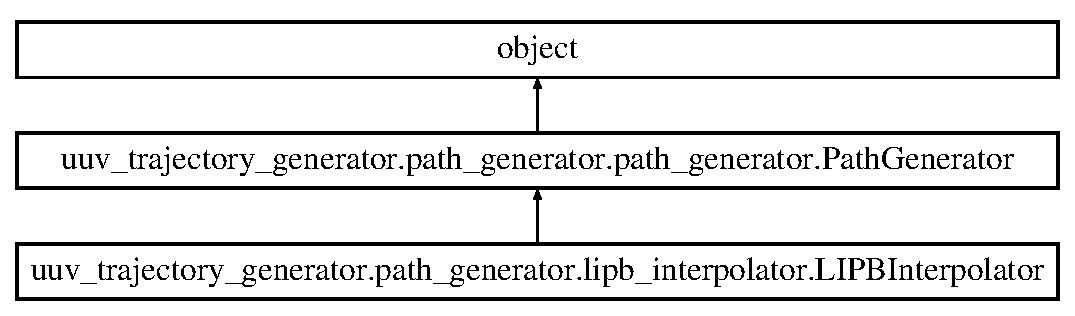
\includegraphics[height=3.000000cm]{classuuv__trajectory__generator_1_1path__generator_1_1lipb__interpolator_1_1LIPBInterpolator}
\end{center}
\end{figure}
\subsection*{Public Member Functions}
\begin{DoxyCompactItemize}
\item 
\mbox{\Hypertarget{classuuv__trajectory__generator_1_1path__generator_1_1lipb__interpolator_1_1LIPBInterpolator_af3cc6ccb8ee6bd08d40a2757938e0f14}\label{classuuv__trajectory__generator_1_1path__generator_1_1lipb__interpolator_1_1LIPBInterpolator_af3cc6ccb8ee6bd08d40a2757938e0f14}} 
def {\bfseries \+\_\+\+\_\+init\+\_\+\+\_\+} (self)
\item 
\mbox{\Hypertarget{classuuv__trajectory__generator_1_1path__generator_1_1lipb__interpolator_1_1LIPBInterpolator_a2490b88875b3a864c7046dc7ee92f003}\label{classuuv__trajectory__generator_1_1path__generator_1_1lipb__interpolator_1_1LIPBInterpolator_a2490b88875b3a864c7046dc7ee92f003}} 
def {\bfseries init\+\_\+interpolator} (self)
\item 
\mbox{\Hypertarget{classuuv__trajectory__generator_1_1path__generator_1_1lipb__interpolator_1_1LIPBInterpolator_aad73f99de216001fb8f7fc9f1eebf023}\label{classuuv__trajectory__generator_1_1path__generator_1_1lipb__interpolator_1_1LIPBInterpolator_aad73f99de216001fb8f7fc9f1eebf023}} 
def {\bfseries set\+\_\+parameters} (self, params)
\item 
\mbox{\Hypertarget{classuuv__trajectory__generator_1_1path__generator_1_1lipb__interpolator_1_1LIPBInterpolator_ad76b24a8d35fea573b558ff4454d8fbd}\label{classuuv__trajectory__generator_1_1path__generator_1_1lipb__interpolator_1_1LIPBInterpolator_ad76b24a8d35fea573b558ff4454d8fbd}} 
def {\bfseries get\+\_\+samples} (self, max\+\_\+time, step=0.\+001)
\item 
\mbox{\Hypertarget{classuuv__trajectory__generator_1_1path__generator_1_1lipb__interpolator_1_1LIPBInterpolator_aaac06a321ee1d0f6f3d5cd579e54027e}\label{classuuv__trajectory__generator_1_1path__generator_1_1lipb__interpolator_1_1LIPBInterpolator_aaac06a321ee1d0f6f3d5cd579e54027e}} 
def {\bfseries generate\+\_\+pos} (self, s, args)
\item 
\mbox{\Hypertarget{classuuv__trajectory__generator_1_1path__generator_1_1lipb__interpolator_1_1LIPBInterpolator_a32dd4fbaa95318bf8efab8bbad522c77}\label{classuuv__trajectory__generator_1_1path__generator_1_1lipb__interpolator_1_1LIPBInterpolator_a32dd4fbaa95318bf8efab8bbad522c77}} 
def {\bfseries generate\+\_\+pnt} (self, s, t=0.\+0, args)
\item 
\mbox{\Hypertarget{classuuv__trajectory__generator_1_1path__generator_1_1lipb__interpolator_1_1LIPBInterpolator_a7a339049eb6d8e76fb0b18f56f314050}\label{classuuv__trajectory__generator_1_1path__generator_1_1lipb__interpolator_1_1LIPBInterpolator_a7a339049eb6d8e76fb0b18f56f314050}} 
def {\bfseries generate\+\_\+quat} (self, s)
\end{DoxyCompactItemize}
\subsection*{Static Public Attributes}
\begin{DoxyCompactItemize}
\item 
\mbox{\Hypertarget{classuuv__trajectory__generator_1_1path__generator_1_1lipb__interpolator_1_1LIPBInterpolator_a0d4bed3882cffbbe5807e5fd81286407}\label{classuuv__trajectory__generator_1_1path__generator_1_1lipb__interpolator_1_1LIPBInterpolator_a0d4bed3882cffbbe5807e5fd81286407}} 
string {\bfseries L\+A\+B\+EL} = \textquotesingle{}lipb\textquotesingle{}
\end{DoxyCompactItemize}
\subsection*{Additional Inherited Members}


\subsection{Detailed Description}
\begin{DoxyVerb}Linear interpolator with polynomial blends.

[1] Biagiotti, Luigi, and Claudio Melchiorri. Trajectory planning for
    automatic machines and robots. Springer Science & Business Media, 2008.
\end{DoxyVerb}
 

The documentation for this class was generated from the following file\+:\begin{DoxyCompactItemize}
\item 
control\+\_\+layer/uuv\+\_\+trajectory\+\_\+control/src/uuv\+\_\+trajectory\+\_\+generator/path\+\_\+generator/lipb\+\_\+interpolator.\+py\end{DoxyCompactItemize}

\hypertarget{classmapping_1_1MappingNode}{}\doxysection{mapping\+::Mapping\+Node Class Reference}
\label{classmapping_1_1MappingNode}\index{mapping::MappingNode@{mapping::MappingNode}}
\doxysubsection*{Public Member Functions}
\begin{DoxyCompactItemize}
\item 
\mbox{\Hypertarget{classmapping_1_1MappingNode_ac5e07918336fbd109fbb80602c112214}\label{classmapping_1_1MappingNode_ac5e07918336fbd109fbb80602c112214}} 
{\bfseries Mapping\+Node} (const ros\+::\+Node\+Handle\+Ptr \&nh)
\item 
\mbox{\Hypertarget{classmapping_1_1MappingNode_ac97adba70e05892c444fdd87aef2fafb}\label{classmapping_1_1MappingNode_ac97adba70e05892c444fdd87aef2fafb}} 
void {\bfseries transform\+\_\+broadcaster\+\_\+initial} (tf\+::\+Transform\+Broadcaster \&map\+\_\+to\+\_\+odom\+\_\+broadcaster)
\item 
\mbox{\Hypertarget{classmapping_1_1MappingNode_a4e4edc5fb06e25d5c6a38ff2aff0e81a}\label{classmapping_1_1MappingNode_a4e4edc5fb06e25d5c6a38ff2aff0e81a}} 
void {\bfseries odometry\+\_\+update\+\_\+cb} (const nav\+\_\+msgs\+::\+Odometry\+::\+Const\+Ptr \&msg)
\item 
\mbox{\Hypertarget{classmapping_1_1MappingNode_a2b033ee1388eacada84c9c4f50db1c36}\label{classmapping_1_1MappingNode_a2b033ee1388eacada84c9c4f50db1c36}} 
void {\bfseries load\+Map\+From\+Y\+A\+ML} (grid\+\_\+map\+::\+Grid\+Map \&map)
\item 
\mbox{\Hypertarget{classmapping_1_1MappingNode_a802e71726ab46853b7d0c79c9b8294cd}\label{classmapping_1_1MappingNode_a802e71726ab46853b7d0c79c9b8294cd}} 
void {\bfseries Publish\+Map} ()
\item 
\mbox{\Hypertarget{classmapping_1_1MappingNode_a84a3cf9f887abfe9d85cb6bd9d96365c}\label{classmapping_1_1MappingNode_a84a3cf9f887abfe9d85cb6bd9d96365c}} 
void {\bfseries Spin} ()
\end{DoxyCompactItemize}


The documentation for this class was generated from the following files\+:\begin{DoxyCompactItemize}
\item 
navigation\+\_\+layer/mapping/include/mapping\+\_\+main.\+h\item 
navigation\+\_\+layer/mapping/src/mapping\+\_\+main.\+cpp\end{DoxyCompactItemize}

\hypertarget{classMarker}{}\doxysection{Marker Class Reference}
\label{classMarker}\index{Marker@{Marker}}
Inheritance diagram for Marker\+:\begin{figure}[H]
\begin{center}
\leavevmode
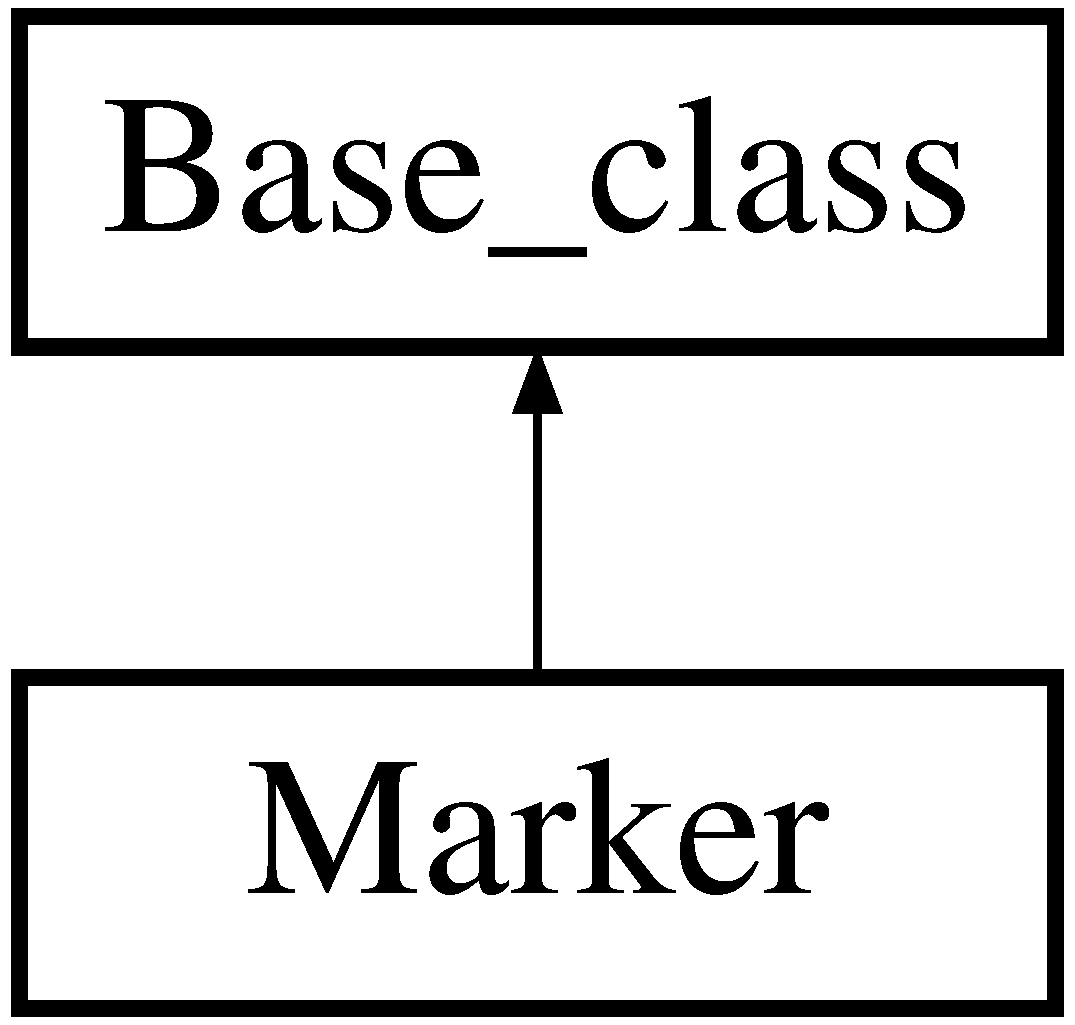
\includegraphics[height=2.000000cm]{classMarker}
\end{center}
\end{figure}
\doxysubsection*{Public Member Functions}
\begin{DoxyCompactItemize}
\item 
\mbox{\Hypertarget{classMarker_abc52521edfd9dabe076335512ee7140c}\label{classMarker_abc52521edfd9dabe076335512ee7140c}} 
virtual void {\bfseries load\+Params} () override
\item 
\mbox{\Hypertarget{classMarker_a3be6e77f4a71adc218ad1a66973f2277}\label{classMarker_a3be6e77f4a71adc218ad1a66973f2277}} 
virtual void {\bfseries spin\+Thread\+Front} () override
\end{DoxyCompactItemize}
\doxysubsection*{Additional Inherited Members}


The documentation for this class was generated from the following files\+:\begin{DoxyCompactItemize}
\item 
vision\+\_\+layer/vision\+\_\+tasks/include/marker.\+h\item 
vision\+\_\+layer/vision\+\_\+tasks/src/marker.\+cpp\end{DoxyCompactItemize}

\hypertarget{classMarkerDropper}{}\section{Marker\+Dropper Class Reference}
\label{classMarkerDropper}\index{Marker\+Dropper@{Marker\+Dropper}}
Inheritance diagram for Marker\+Dropper\+:\begin{figure}[H]
\begin{center}
\leavevmode
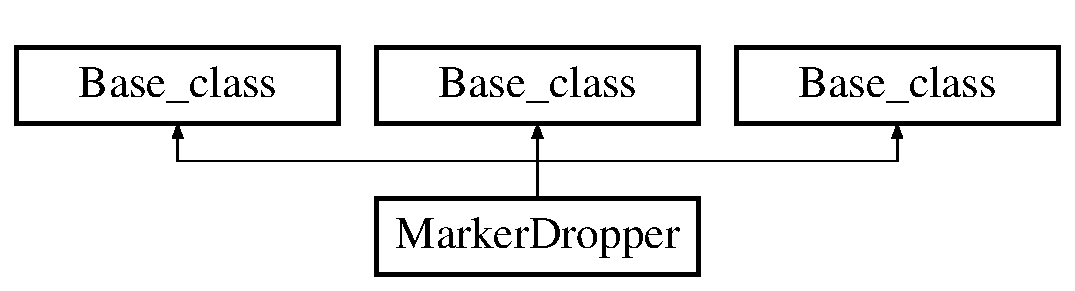
\includegraphics[height=2.000000cm]{classMarkerDropper}
\end{center}
\end{figure}
\subsection*{Public Member Functions}
\begin{DoxyCompactItemize}
\item 
\mbox{\Hypertarget{classMarkerDropper_a60c7e60403cdcbd33d50c9bae3309b65}\label{classMarkerDropper_a60c7e60403cdcbd33d50c9bae3309b65}} 
virtual void {\bfseries load\+Params} () override
\item 
\mbox{\Hypertarget{classMarkerDropper_abb62612d590e6ea50503d489cb1b41aa}\label{classMarkerDropper_abb62612d590e6ea50503d489cb1b41aa}} 
virtual void {\bfseries spin\+Thread\+Bottom} () override
\item 
\mbox{\Hypertarget{classMarkerDropper_aa9bf73390dc56ebe4827a6c27167fe9b}\label{classMarkerDropper_aa9bf73390dc56ebe4827a6c27167fe9b}} 
void {\bfseries pre\+Process} (cv\+::\+Mat \&temp\+\_\+src)
\item 
\mbox{\Hypertarget{classMarkerDropper_aff48227552a1737e8dd8591b61293233}\label{classMarkerDropper_aff48227552a1737e8dd8591b61293233}} 
cv\+::\+Point {\bfseries find\+Center} ()
\item 
\mbox{\Hypertarget{classMarkerDropper_ab2707be25d4882e94838ec4a9ff2aba8}\label{classMarkerDropper_ab2707be25d4882e94838ec4a9ff2aba8}} 
void {\bfseries spin\+Thread\+Bottom} ()
\item 
\mbox{\Hypertarget{classMarkerDropper_a1b9b487b4fc201977a35e35bdd083667}\label{classMarkerDropper_a1b9b487b4fc201977a35e35bdd083667}} 
void {\bfseries spin\+Thread\+Front} ()
\item 
\mbox{\Hypertarget{classMarkerDropper_ab2707be25d4882e94838ec4a9ff2aba8}\label{classMarkerDropper_ab2707be25d4882e94838ec4a9ff2aba8}} 
void {\bfseries spin\+Thread\+Bottom} ()
\item 
\mbox{\Hypertarget{classMarkerDropper_a1b9b487b4fc201977a35e35bdd083667}\label{classMarkerDropper_a1b9b487b4fc201977a35e35bdd083667}} 
void {\bfseries spin\+Thread\+Front} ()
\end{DoxyCompactItemize}
\subsection*{Public Attributes}
\begin{DoxyCompactItemize}
\item 
\mbox{\Hypertarget{classMarkerDropper_a596c0798e6b5baf6afb72d0191cfa12c}\label{classMarkerDropper_a596c0798e6b5baf6afb72d0191cfa12c}} 
cv\+::\+Mat {\bfseries image\+\_\+marked}
\end{DoxyCompactItemize}
\subsection*{Protected Member Functions}
\begin{DoxyCompactItemize}
\item 
\mbox{\Hypertarget{classMarkerDropper_acdf8f8e4b2d8fde47651b3814f20d47d}\label{classMarkerDropper_acdf8f8e4b2d8fde47651b3814f20d47d}} 
void {\bfseries front\+Callback} (vision\+\_\+tasks\+::marker\+Dropper\+Front\+Range\+Config \&config, double level)
\item 
\mbox{\Hypertarget{classMarkerDropper_acbc9da12d06e0bdb7d659982d814c959}\label{classMarkerDropper_acbc9da12d06e0bdb7d659982d814c959}} 
void {\bfseries bottom\+Callback} (vision\+\_\+tasks\+::marker\+Dropper\+Bottom\+Range\+Config \&config, double level)
\item 
\mbox{\Hypertarget{classMarkerDropper_a65a611716c6e3f35510534e4c07080ef}\label{classMarkerDropper_a65a611716c6e3f35510534e4c07080ef}} 
void {\bfseries image\+Front\+Callback} (const sensor\+\_\+msgs\+::\+Image\+::\+Const\+Ptr \&msg)
\item 
\mbox{\Hypertarget{classMarkerDropper_af1d127a6a637b618cc71d42447a9e8c2}\label{classMarkerDropper_af1d127a6a637b618cc71d42447a9e8c2}} 
void {\bfseries image\+Bottom\+Callback} (const sensor\+\_\+msgs\+::\+Image\+::\+Const\+Ptr \&msg)
\item 
\mbox{\Hypertarget{classMarkerDropper_acdf8f8e4b2d8fde47651b3814f20d47d}\label{classMarkerDropper_acdf8f8e4b2d8fde47651b3814f20d47d}} 
void {\bfseries front\+Callback} (vision\+\_\+tasks\+::marker\+Dropper\+Front\+Range\+Config \&config, double level)
\item 
\mbox{\Hypertarget{classMarkerDropper_acbc9da12d06e0bdb7d659982d814c959}\label{classMarkerDropper_acbc9da12d06e0bdb7d659982d814c959}} 
void {\bfseries bottom\+Callback} (vision\+\_\+tasks\+::marker\+Dropper\+Bottom\+Range\+Config \&config, double level)
\item 
\mbox{\Hypertarget{classMarkerDropper_a65a611716c6e3f35510534e4c07080ef}\label{classMarkerDropper_a65a611716c6e3f35510534e4c07080ef}} 
void {\bfseries image\+Front\+Callback} (const sensor\+\_\+msgs\+::\+Image\+::\+Const\+Ptr \&msg)
\item 
\mbox{\Hypertarget{classMarkerDropper_af1d127a6a637b618cc71d42447a9e8c2}\label{classMarkerDropper_af1d127a6a637b618cc71d42447a9e8c2}} 
void {\bfseries image\+Bottom\+Callback} (const sensor\+\_\+msgs\+::\+Image\+::\+Const\+Ptr \&msg)
\end{DoxyCompactItemize}
\subsection*{Protected Attributes}
\begin{DoxyCompactItemize}
\item 
\mbox{\Hypertarget{classMarkerDropper_a46f35c9468e60bbf6b0804daee3b501b}\label{classMarkerDropper_a46f35c9468e60bbf6b0804daee3b501b}} 
image\+\_\+transport\+::\+Publisher {\bfseries bottom\+\_\+blue\+\_\+filtered\+\_\+pub}
\item 
\mbox{\Hypertarget{classMarkerDropper_af48c1237b7c61106f7e86c947ef7e0e8}\label{classMarkerDropper_af48c1237b7c61106f7e86c947ef7e0e8}} 
image\+\_\+transport\+::\+Publisher {\bfseries front\+\_\+blue\+\_\+filtered\+\_\+pub}
\item 
\mbox{\Hypertarget{classMarkerDropper_a4a5cd2eee6cda56ce177632b446a21cc}\label{classMarkerDropper_a4a5cd2eee6cda56ce177632b446a21cc}} 
image\+\_\+transport\+::\+Subscriber {\bfseries front\+\_\+image\+\_\+raw\+\_\+sub}
\item 
\mbox{\Hypertarget{classMarkerDropper_ab05e2f71e55e15d2d40bec83aec09e5c}\label{classMarkerDropper_ab05e2f71e55e15d2d40bec83aec09e5c}} 
image\+\_\+transport\+::\+Subscriber {\bfseries bottom\+\_\+image\+\_\+raw\+\_\+sub}
\item 
\mbox{\Hypertarget{classMarkerDropper_a4bda362c08b94bc38433f430c8dce643}\label{classMarkerDropper_a4bda362c08b94bc38433f430c8dce643}} 
ros\+::\+Publisher {\bfseries detection\+\_\+pub}
\item 
\mbox{\Hypertarget{classMarkerDropper_a12e2db834779b18197b7c5d541f5f566}\label{classMarkerDropper_a12e2db834779b18197b7c5d541f5f566}} 
std\+::string {\bfseries camera\+\_\+frame\+\_\+}
\item 
\mbox{\Hypertarget{classMarkerDropper_aa98a4125b058fcf57bbed17ee12678e2}\label{classMarkerDropper_aa98a4125b058fcf57bbed17ee12678e2}} 
double {\bfseries front\+\_\+clahe\+\_\+clip\+\_\+} = 4.\+0
\item 
\mbox{\Hypertarget{classMarkerDropper_a23c3cd5e393d5fca8d76f7eaf596804d}\label{classMarkerDropper_a23c3cd5e393d5fca8d76f7eaf596804d}} 
int {\bfseries front\+\_\+clahe\+\_\+grid\+\_\+size\+\_\+} = 8
\item 
\mbox{\Hypertarget{classMarkerDropper_a69a9bd6730222d56dee1707c2e5dd599}\label{classMarkerDropper_a69a9bd6730222d56dee1707c2e5dd599}} 
int {\bfseries front\+\_\+clahe\+\_\+bilateral\+\_\+iter\+\_\+} = 8
\item 
\mbox{\Hypertarget{classMarkerDropper_a2c7cf4b4b24406a7d684f276fe02b763}\label{classMarkerDropper_a2c7cf4b4b24406a7d684f276fe02b763}} 
int {\bfseries front\+\_\+balanced\+\_\+bilateral\+\_\+iter\+\_\+} = 4
\item 
\mbox{\Hypertarget{classMarkerDropper_a576351ceb624124a9f177e4aa10e72b0}\label{classMarkerDropper_a576351ceb624124a9f177e4aa10e72b0}} 
double {\bfseries front\+\_\+denoise\+\_\+h\+\_\+} = 10.\+0
\item 
\mbox{\Hypertarget{classMarkerDropper_a97e708ac1dc23f14efe48c64e3eb0496}\label{classMarkerDropper_a97e708ac1dc23f14efe48c64e3eb0496}} 
int {\bfseries front\+\_\+canny\+\_\+threshold\+\_\+low\+\_\+} = 0
\item 
\mbox{\Hypertarget{classMarkerDropper_ada1f7cb1f635913c6b9612fa890526af}\label{classMarkerDropper_ada1f7cb1f635913c6b9612fa890526af}} 
int {\bfseries front\+\_\+canny\+\_\+threshold\+\_\+high\+\_\+} = 1000
\item 
\mbox{\Hypertarget{classMarkerDropper_aa3d54dfdca7a35d676e0036f085bf14f}\label{classMarkerDropper_aa3d54dfdca7a35d676e0036f085bf14f}} 
int {\bfseries front\+\_\+canny\+\_\+kernel\+\_\+size\+\_\+} = 3
\item 
\mbox{\Hypertarget{classMarkerDropper_abca1ba7eace809915a9c674cc9134a28}\label{classMarkerDropper_abca1ba7eace809915a9c674cc9134a28}} 
int {\bfseries front\+\_\+hough\+\_\+threshold\+\_\+} = 0
\item 
\mbox{\Hypertarget{classMarkerDropper_a96fb9649f9d3c5d94e99705ec8c70f52}\label{classMarkerDropper_a96fb9649f9d3c5d94e99705ec8c70f52}} 
int {\bfseries front\+\_\+hough\+\_\+minline\+\_\+} = 0
\item 
\mbox{\Hypertarget{classMarkerDropper_aba7342ce88e06358356298b4fd4c797f}\label{classMarkerDropper_aba7342ce88e06358356298b4fd4c797f}} 
int {\bfseries front\+\_\+hough\+\_\+maxgap\+\_\+} = 0
\item 
\mbox{\Hypertarget{classMarkerDropper_a5cce65c39a401bd6d966d3449c990960}\label{classMarkerDropper_a5cce65c39a401bd6d966d3449c990960}} 
double {\bfseries front\+\_\+hough\+\_\+angle\+\_\+tolerance\+\_\+} = 0.\+0
\item 
\mbox{\Hypertarget{classMarkerDropper_a01d2f9bee667f199b5bc2e8f55ef0ca9}\label{classMarkerDropper_a01d2f9bee667f199b5bc2e8f55ef0ca9}} 
double {\bfseries front\+\_\+gate\+\_\+distance\+\_\+tolerance\+\_\+} = 50.\+0
\item 
\mbox{\Hypertarget{classMarkerDropper_a5c2afc4167d551e1854fcad96398703f}\label{classMarkerDropper_a5c2afc4167d551e1854fcad96398703f}} 
double {\bfseries front\+\_\+gate\+\_\+angle\+\_\+tolerance\+\_\+} = 0.\+0
\item 
\mbox{\Hypertarget{classMarkerDropper_ab1f4f4ed6a0691eaaf24e1f0bb8c20ed}\label{classMarkerDropper_ab1f4f4ed6a0691eaaf24e1f0bb8c20ed}} 
double {\bfseries bottom\+\_\+clahe\+\_\+clip\+\_\+} = 4.\+0
\item 
\mbox{\Hypertarget{classMarkerDropper_a97f2c6dd6b1cffa4ac7ee3a03c42edd0}\label{classMarkerDropper_a97f2c6dd6b1cffa4ac7ee3a03c42edd0}} 
int {\bfseries bottom\+\_\+clahe\+\_\+grid\+\_\+size\+\_\+} = 8
\item 
\mbox{\Hypertarget{classMarkerDropper_a1b87c6207ae2f9b5be1252c80f6a2f29}\label{classMarkerDropper_a1b87c6207ae2f9b5be1252c80f6a2f29}} 
int {\bfseries bottom\+\_\+clahe\+\_\+bilateral\+\_\+iter\+\_\+} = 8
\item 
\mbox{\Hypertarget{classMarkerDropper_a8ec68edd01310878f1313c6d5c26ae12}\label{classMarkerDropper_a8ec68edd01310878f1313c6d5c26ae12}} 
int {\bfseries bottom\+\_\+balanced\+\_\+bilateral\+\_\+iter\+\_\+} = 4
\item 
\mbox{\Hypertarget{classMarkerDropper_ab73c9b6e3cc690545ab81a47595ccc89}\label{classMarkerDropper_ab73c9b6e3cc690545ab81a47595ccc89}} 
double {\bfseries bottom\+\_\+denoise\+\_\+h\+\_\+} = 10.\+0
\end{DoxyCompactItemize}


The documentation for this class was generated from the following files\+:\begin{DoxyCompactItemize}
\item 
vision\+\_\+layer/vision\+\_\+tasks/include/marker\+\_\+dropper.\+h\item 
vision\+\_\+layer/vision\+\_\+tasks/include/marker\+Dropper.\+h\item 
vision\+\_\+layer/vision\+\_\+tasks/include/marker\+Dropper\+\_\+niot.\+h\item 
vision\+\_\+layer/vision\+\_\+tasks/src/marker\+\_\+dropper.\+cpp\item 
vision\+\_\+layer/vision\+\_\+tasks/src/marker\+Dropper.\+cpp\item 
vision\+\_\+layer/vision\+\_\+tasks/src/marker\+Dropper\+\_\+niot.\+cpp\end{DoxyCompactItemize}

\hypertarget{classmaster__layer_1_1state__mach_1_1MarkerDropperTask}{}\section{master\+\_\+layer.\+state\+\_\+mach.\+Marker\+Dropper\+Task Class Reference}
\label{classmaster__layer_1_1state__mach_1_1MarkerDropperTask}\index{master\+\_\+layer.\+state\+\_\+mach.\+Marker\+Dropper\+Task@{master\+\_\+layer.\+state\+\_\+mach.\+Marker\+Dropper\+Task}}
Inheritance diagram for master\+\_\+layer.\+state\+\_\+mach.\+Marker\+Dropper\+Task\+:\begin{figure}[H]
\begin{center}
\leavevmode
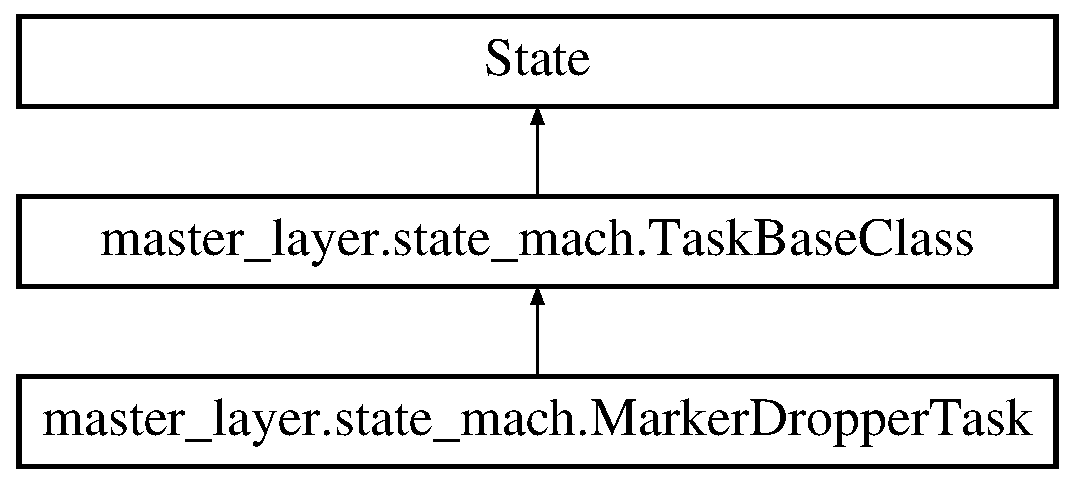
\includegraphics[height=3.000000cm]{classmaster__layer_1_1state__mach_1_1MarkerDropperTask}
\end{center}
\end{figure}
\subsection*{Public Member Functions}
\begin{DoxyCompactItemize}
\item 
\mbox{\Hypertarget{classmaster__layer_1_1state__mach_1_1MarkerDropperTask_aeaee4f4556ded94b0c4c714fd36cef3d}\label{classmaster__layer_1_1state__mach_1_1MarkerDropperTask_aeaee4f4556ded94b0c4c714fd36cef3d}} 
def {\bfseries \+\_\+\+\_\+init\+\_\+\+\_\+} (self)
\item 
\mbox{\Hypertarget{classmaster__layer_1_1state__mach_1_1MarkerDropperTask_a4f87206008f89058c4745cb69d43d7fc}\label{classmaster__layer_1_1state__mach_1_1MarkerDropperTask_a4f87206008f89058c4745cb69d43d7fc}} 
def {\bfseries align} (self)
\item 
\mbox{\Hypertarget{classmaster__layer_1_1state__mach_1_1MarkerDropperTask_aa334686bbb38eb471793471c81264218}\label{classmaster__layer_1_1state__mach_1_1MarkerDropperTask_aa334686bbb38eb471793471c81264218}} 
def {\bfseries execute} (self)
\end{DoxyCompactItemize}


The documentation for this class was generated from the following file\+:\begin{DoxyCompactItemize}
\item 
master\+\_\+layer/src/master\+\_\+layer/state\+\_\+mach.\+py\end{DoxyCompactItemize}

\hypertarget{classmaster__layer_1_1state__mach__gate__torpedo_1_1MarkerDropperTask}{}\doxysection{master\+\_\+layer.\+state\+\_\+mach\+\_\+gate\+\_\+torpedo.\+Marker\+Dropper\+Task Class Reference}
\label{classmaster__layer_1_1state__mach__gate__torpedo_1_1MarkerDropperTask}\index{master\_layer.state\_mach\_gate\_torpedo.MarkerDropperTask@{master\_layer.state\_mach\_gate\_torpedo.MarkerDropperTask}}
Inheritance diagram for master\+\_\+layer.\+state\+\_\+mach\+\_\+gate\+\_\+torpedo.\+Marker\+Dropper\+Task\+:\begin{figure}[H]
\begin{center}
\leavevmode
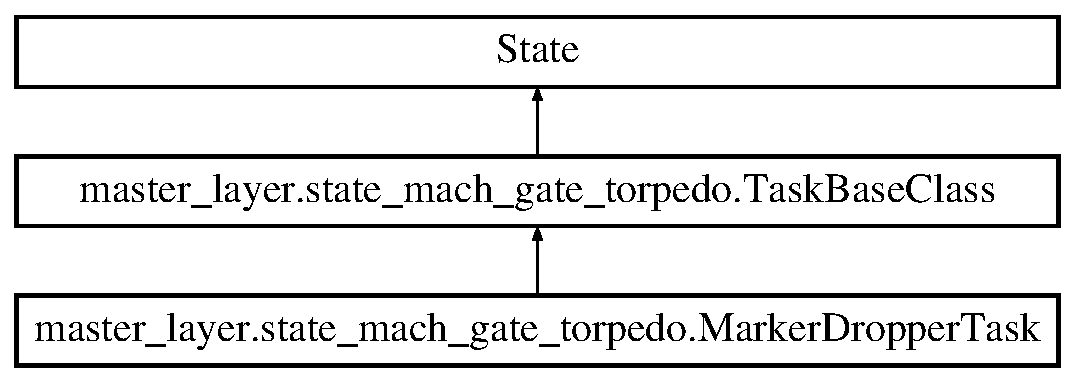
\includegraphics[height=3.000000cm]{classmaster__layer_1_1state__mach__gate__torpedo_1_1MarkerDropperTask}
\end{center}
\end{figure}
\doxysubsection*{Public Member Functions}
\begin{DoxyCompactItemize}
\item 
\mbox{\Hypertarget{classmaster__layer_1_1state__mach__gate__torpedo_1_1MarkerDropperTask_a51d7db6f46c0a8cf283320f26d2f6c7f}\label{classmaster__layer_1_1state__mach__gate__torpedo_1_1MarkerDropperTask_a51d7db6f46c0a8cf283320f26d2f6c7f}} 
def {\bfseries \+\_\+\+\_\+init\+\_\+\+\_\+} (self)
\item 
\mbox{\Hypertarget{classmaster__layer_1_1state__mach__gate__torpedo_1_1MarkerDropperTask_a86aae57d8f860d9875c2dc8a7387cff6}\label{classmaster__layer_1_1state__mach__gate__torpedo_1_1MarkerDropperTask_a86aae57d8f860d9875c2dc8a7387cff6}} 
def {\bfseries align} (self)
\item 
\mbox{\Hypertarget{classmaster__layer_1_1state__mach__gate__torpedo_1_1MarkerDropperTask_adac8439216ad70cd3424f46129d6e2a0}\label{classmaster__layer_1_1state__mach__gate__torpedo_1_1MarkerDropperTask_adac8439216ad70cd3424f46129d6e2a0}} 
def {\bfseries execute} (self)
\end{DoxyCompactItemize}


The documentation for this class was generated from the following file\+:\begin{DoxyCompactItemize}
\item 
master\+\_\+layer/src/master\+\_\+layer/state\+\_\+mach\+\_\+gate\+\_\+torpedo.\+py\end{DoxyCompactItemize}

\hypertarget{classcolor__correction_1_1max__edge}{}\section{color\+\_\+correction\+:\+:max\+\_\+edge Class Reference}
\label{classcolor__correction_1_1max__edge}\index{color\+\_\+correction\+::max\+\_\+edge@{color\+\_\+correction\+::max\+\_\+edge}}
\subsection*{Public Types}
\begin{DoxyCompactItemize}
\item 
enum \hyperlink{classcolor__correction_1_1max__edge_af83c7bb6554486a755ba5133a427acc0}{Convolution\+Type} \{ {\bfseries C\+O\+N\+V\+O\+L\+U\+T\+I\+O\+N\+\_\+\+F\+U\+LL}, 
{\bfseries C\+O\+N\+V\+O\+L\+U\+T\+I\+O\+N\+\_\+\+S\+A\+ME}, 
{\bfseries C\+O\+N\+V\+O\+L\+U\+T\+I\+O\+N\+\_\+\+V\+A\+L\+ID}
 \}
\end{DoxyCompactItemize}
\subsection*{Public Member Functions}
\begin{DoxyCompactItemize}
\item 
Mat \hyperlink{classcolor__correction_1_1max__edge_ab986a6eeda0ae54621f48b1a3acde38d}{run} (Mat, int p, int m)
\item 
void \hyperlink{classcolor__correction_1_1max__edge_af9ab5e0868c8e3d667ed63c03f6cf850}{conv2} (const Mat \&img, const Mat \&kernel, \hyperlink{classcolor__correction_1_1max__edge_af83c7bb6554486a755ba5133a427acc0}{Convolution\+Type} type, Mat \&dest)
\item 
void \hyperlink{classcolor__correction_1_1max__edge_a1d72dd0a81e84d809dd2da19342f42a8}{process} (Mat src1, float $\ast$ml, float $\ast$ma, float $\ast$mb, int p, int m)
\end{DoxyCompactItemize}


\subsection{Member Enumeration Documentation}
\mbox{\Hypertarget{classcolor__correction_1_1max__edge_af83c7bb6554486a755ba5133a427acc0}\label{classcolor__correction_1_1max__edge_af83c7bb6554486a755ba5133a427acc0}} 
\index{color\+\_\+correction\+::max\+\_\+edge@{color\+\_\+correction\+::max\+\_\+edge}!Convolution\+Type@{Convolution\+Type}}
\index{Convolution\+Type@{Convolution\+Type}!color\+\_\+correction\+::max\+\_\+edge@{color\+\_\+correction\+::max\+\_\+edge}}
\subsubsection{\texorpdfstring{Convolution\+Type}{ConvolutionType}}
{\footnotesize\ttfamily enum \hyperlink{classcolor__correction_1_1max__edge_af83c7bb6554486a755ba5133a427acc0}{color\+\_\+correction\+::max\+\_\+edge\+::\+Convolution\+Type}}

defines convolution type 

\subsection{Member Function Documentation}
\mbox{\Hypertarget{classcolor__correction_1_1max__edge_af9ab5e0868c8e3d667ed63c03f6cf850}\label{classcolor__correction_1_1max__edge_af9ab5e0868c8e3d667ed63c03f6cf850}} 
\index{color\+\_\+correction\+::max\+\_\+edge@{color\+\_\+correction\+::max\+\_\+edge}!conv2@{conv2}}
\index{conv2@{conv2}!color\+\_\+correction\+::max\+\_\+edge@{color\+\_\+correction\+::max\+\_\+edge}}
\subsubsection{\texorpdfstring{conv2()}{conv2()}}
{\footnotesize\ttfamily void color\+\_\+correction\+::max\+\_\+edge\+::conv2 (\begin{DoxyParamCaption}\item[{const Mat \&}]{img,  }\item[{const Mat \&}]{kernel,  }\item[{\hyperlink{classcolor__correction_1_1max__edge_af83c7bb6554486a755ba5133a427acc0}{Convolution\+Type}}]{type,  }\item[{Mat \&}]{dest }\end{DoxyParamCaption})}

method to perform 2D convolution \mbox{\Hypertarget{classcolor__correction_1_1max__edge_a1d72dd0a81e84d809dd2da19342f42a8}\label{classcolor__correction_1_1max__edge_a1d72dd0a81e84d809dd2da19342f42a8}} 
\index{color\+\_\+correction\+::max\+\_\+edge@{color\+\_\+correction\+::max\+\_\+edge}!process@{process}}
\index{process@{process}!color\+\_\+correction\+::max\+\_\+edge@{color\+\_\+correction\+::max\+\_\+edge}}
\subsubsection{\texorpdfstring{process()}{process()}}
{\footnotesize\ttfamily void color\+\_\+correction\+::max\+\_\+edge\+::process (\begin{DoxyParamCaption}\item[{Mat}]{src1,  }\item[{float $\ast$}]{ml,  }\item[{float $\ast$}]{ma,  }\item[{float $\ast$}]{mb,  }\item[{int}]{p,  }\item[{int}]{m }\end{DoxyParamCaption})}

function that computes illumination vector for \hyperlink{classcolor__correction_1_1max__edge}{max\+\_\+edge} algorithm \mbox{\Hypertarget{classcolor__correction_1_1max__edge_ab986a6eeda0ae54621f48b1a3acde38d}\label{classcolor__correction_1_1max__edge_ab986a6eeda0ae54621f48b1a3acde38d}} 
\index{color\+\_\+correction\+::max\+\_\+edge@{color\+\_\+correction\+::max\+\_\+edge}!run@{run}}
\index{run@{run}!color\+\_\+correction\+::max\+\_\+edge@{color\+\_\+correction\+::max\+\_\+edge}}
\subsubsection{\texorpdfstring{run()}{run()}}
{\footnotesize\ttfamily Mat color\+\_\+correction\+::max\+\_\+edge\+::run (\begin{DoxyParamCaption}\item[{Mat}]{src1,  }\item[{int}]{p,  }\item[{int}]{m }\end{DoxyParamCaption})}

main function to call to perform max-\/edge color correction 

The documentation for this class was generated from the following files\+:\begin{DoxyCompactItemize}
\item 
vision\+\_\+layer/vision\+\_\+fusion/include/fusion/color\+\_\+constancy.\+hpp\item 
vision\+\_\+layer/vision\+\_\+fusion/src/color\+\_\+constancy.\+cpp\end{DoxyCompactItemize}

\hypertarget{classcolor__correction_1_1maxRGB}{}\doxysection{color\+\_\+correction\+::max\+R\+GB Class Reference}
\label{classcolor__correction_1_1maxRGB}\index{color\_correction::maxRGB@{color\_correction::maxRGB}}
\doxysubsection*{Public Member Functions}
\begin{DoxyCompactItemize}
\item 
Mat \mbox{\hyperlink{classcolor__correction_1_1maxRGB_acf7ab1043e266c02f54d83b8c5625284}{run}} (Mat, int p, int m)
\item 
void \mbox{\hyperlink{classcolor__correction_1_1maxRGB_a7da874962b27949e521c065d56354264}{process}} (Mat src1, float $\ast$ml, float $\ast$ma, float $\ast$mb, int p, int m)
\end{DoxyCompactItemize}


\doxysubsection{Member Function Documentation}
\mbox{\Hypertarget{classcolor__correction_1_1maxRGB_a7da874962b27949e521c065d56354264}\label{classcolor__correction_1_1maxRGB_a7da874962b27949e521c065d56354264}} 
\index{color\_correction::maxRGB@{color\_correction::maxRGB}!process@{process}}
\index{process@{process}!color\_correction::maxRGB@{color\_correction::maxRGB}}
\doxysubsubsection{\texorpdfstring{process()}{process()}}
{\footnotesize\ttfamily void color\+\_\+correction\+::max\+R\+G\+B\+::process (\begin{DoxyParamCaption}\item[{Mat}]{src1,  }\item[{float $\ast$}]{ml,  }\item[{float $\ast$}]{ma,  }\item[{float $\ast$}]{mb,  }\item[{int}]{p,  }\item[{int}]{m }\end{DoxyParamCaption})}

function coputes the illumination estimate max R\+GB algorithm.\+The function takes input image,minkowski norm and normalization method . the output are ml,,ma,mb for each of the color channels \mbox{\Hypertarget{classcolor__correction_1_1maxRGB_acf7ab1043e266c02f54d83b8c5625284}\label{classcolor__correction_1_1maxRGB_acf7ab1043e266c02f54d83b8c5625284}} 
\index{color\_correction::maxRGB@{color\_correction::maxRGB}!run@{run}}
\index{run@{run}!color\_correction::maxRGB@{color\_correction::maxRGB}}
\doxysubsubsection{\texorpdfstring{run()}{run()}}
{\footnotesize\ttfamily Mat color\+\_\+correction\+::max\+R\+G\+B\+::run (\begin{DoxyParamCaption}\item[{Mat}]{src1,  }\item[{int}]{p,  }\item[{int}]{m }\end{DoxyParamCaption})}

main function to call for \mbox{\hyperlink{classcolor__correction_1_1maxRGB}{max\+R\+GB}} color correction 

The documentation for this class was generated from the following files\+:\begin{DoxyCompactItemize}
\item 
vision\+\_\+layer/vision\+\_\+fusion/include/fusion/color\+\_\+constancy.\+hpp\item 
vision\+\_\+layer/vision\+\_\+fusion/src/color\+\_\+constancy.\+cpp\end{DoxyCompactItemize}

\hypertarget{classmtdef_1_1MID}{}\section{mtdef.\+M\+ID Class Reference}
\label{classmtdef_1_1MID}\index{mtdef.\+M\+ID@{mtdef.\+M\+ID}}
\subsection*{Static Public Attributes}
\begin{DoxyCompactItemize}
\item 
\mbox{\Hypertarget{classmtdef_1_1MID_a608e56ed598132190aaf01ba780dcab1}\label{classmtdef_1_1MID_a608e56ed598132190aaf01ba780dcab1}} 
int {\bfseries Error} = 0x42
\item 
\mbox{\Hypertarget{classmtdef_1_1MID_ad104a29eb3990dae3a392a7cc5ba7c95}\label{classmtdef_1_1MID_ad104a29eb3990dae3a392a7cc5ba7c95}} 
int {\bfseries Wake\+Up} = 0x3E
\item 
\mbox{\Hypertarget{classmtdef_1_1MID_a12491a02c68fb39dd1698a1bdcac8e0e}\label{classmtdef_1_1MID_a12491a02c68fb39dd1698a1bdcac8e0e}} 
int {\bfseries Wake\+Up\+Ack} = 0x3F
\item 
\mbox{\Hypertarget{classmtdef_1_1MID_ad7b3e2db2289b8797835b03db4ac43f9}\label{classmtdef_1_1MID_ad7b3e2db2289b8797835b03db4ac43f9}} 
int {\bfseries Go\+To\+Config} = 0x30
\item 
\mbox{\Hypertarget{classmtdef_1_1MID_a04e17ffd654afb91678099f6199f3c37}\label{classmtdef_1_1MID_a04e17ffd654afb91678099f6199f3c37}} 
int {\bfseries Go\+To\+Measurement} = 0x10
\item 
\mbox{\Hypertarget{classmtdef_1_1MID_ae9fd1db62b90f7837e1a15f8dd827d80}\label{classmtdef_1_1MID_ae9fd1db62b90f7837e1a15f8dd827d80}} 
int {\bfseries Reset} = 0x40
\item 
\mbox{\Hypertarget{classmtdef_1_1MID_acffae763edc788f54a336718115c496e}\label{classmtdef_1_1MID_acffae763edc788f54a336718115c496e}} 
int {\bfseries Req\+D\+ID} = 0x00
\item 
\mbox{\Hypertarget{classmtdef_1_1MID_a3f8fa7b6d3da3f699339804a7e2b071e}\label{classmtdef_1_1MID_a3f8fa7b6d3da3f699339804a7e2b071e}} 
int {\bfseries Device\+ID} = 0x01
\item 
\mbox{\Hypertarget{classmtdef_1_1MID_a9ff2f0fa2cf5c3efbf710307b9ac782a}\label{classmtdef_1_1MID_a9ff2f0fa2cf5c3efbf710307b9ac782a}} 
int {\bfseries Req\+Product\+Code} = 0x1C
\item 
\mbox{\Hypertarget{classmtdef_1_1MID_ac4ec4d43af4de52721a339f5fb91ebcf}\label{classmtdef_1_1MID_ac4ec4d43af4de52721a339f5fb91ebcf}} 
int {\bfseries Product\+Code} = 0x1D
\item 
\mbox{\Hypertarget{classmtdef_1_1MID_aedcad0c6da51367cfcb83bb487cae8dd}\label{classmtdef_1_1MID_aedcad0c6da51367cfcb83bb487cae8dd}} 
int {\bfseries Req\+F\+W\+Rev} = 0x12
\item 
\mbox{\Hypertarget{classmtdef_1_1MID_adb48e1746366ebd8d89d68197f68378d}\label{classmtdef_1_1MID_adb48e1746366ebd8d89d68197f68378d}} 
int {\bfseries Firmware\+Rev} = 0x13
\item 
\mbox{\Hypertarget{classmtdef_1_1MID_ab52b74506bfc605ec7ec6e5e2c7e1e1c}\label{classmtdef_1_1MID_ab52b74506bfc605ec7ec6e5e2c7e1e1c}} 
int {\bfseries Restore\+Factory\+Def} = 0x0E
\item 
\mbox{\Hypertarget{classmtdef_1_1MID_a037d7b2c8172c771815abe1119f01922}\label{classmtdef_1_1MID_a037d7b2c8172c771815abe1119f01922}} 
int {\bfseries Set\+Baudrate} = 0x18
\item 
\mbox{\Hypertarget{classmtdef_1_1MID_a105f221a1a955c81118f859cce8fafeb}\label{classmtdef_1_1MID_a105f221a1a955c81118f859cce8fafeb}} 
int {\bfseries Run\+Selftest} = 0x24
\item 
\mbox{\Hypertarget{classmtdef_1_1MID_ad7c8e2cd3e1cd377940c7b17b2712fa3}\label{classmtdef_1_1MID_ad7c8e2cd3e1cd377940c7b17b2712fa3}} 
int {\bfseries Selftest\+Ack} = 0x25
\item 
\mbox{\Hypertarget{classmtdef_1_1MID_a552c6cb9926047afbdbd1748f80d4911}\label{classmtdef_1_1MID_a552c6cb9926047afbdbd1748f80d4911}} 
int {\bfseries Set\+Error\+Mode} = 0x\+DA
\item 
\mbox{\Hypertarget{classmtdef_1_1MID_a1ac2067125707c27654a8caf29311391}\label{classmtdef_1_1MID_a1ac2067125707c27654a8caf29311391}} 
int {\bfseries Set\+Transmit\+Delay} = 0x\+DC
\item 
\mbox{\Hypertarget{classmtdef_1_1MID_a606c40fd1c39ee814b65b5ea194b24b4}\label{classmtdef_1_1MID_a606c40fd1c39ee814b65b5ea194b24b4}} 
int {\bfseries Set\+Option\+Flags} = 0x48
\item 
\mbox{\Hypertarget{classmtdef_1_1MID_a550c7b7d02a4c88284acb1ffb95dd9ab}\label{classmtdef_1_1MID_a550c7b7d02a4c88284acb1ffb95dd9ab}} 
int {\bfseries Set\+Location\+ID} = 0x84
\item 
\mbox{\Hypertarget{classmtdef_1_1MID_a4e0aee69829d488c550b14a05087524d}\label{classmtdef_1_1MID_a4e0aee69829d488c550b14a05087524d}} 
int {\bfseries Set\+Sync\+Settings} = 0x2C
\item 
\mbox{\Hypertarget{classmtdef_1_1MID_af18b38f2c0da70402dc48a48fd110d15}\label{classmtdef_1_1MID_af18b38f2c0da70402dc48a48fd110d15}} 
int {\bfseries Req\+Configuration} = 0x0C
\item 
\mbox{\Hypertarget{classmtdef_1_1MID_ab1858abfb053a0eaa3bd69f1d56acecd}\label{classmtdef_1_1MID_ab1858abfb053a0eaa3bd69f1d56acecd}} 
int {\bfseries Configuration} = 0x0D
\item 
\mbox{\Hypertarget{classmtdef_1_1MID_a8a11769a3e6c257fcc5c360d67e03a5d}\label{classmtdef_1_1MID_a8a11769a3e6c257fcc5c360d67e03a5d}} 
int {\bfseries Set\+Period} = 0x04
\item 
\mbox{\Hypertarget{classmtdef_1_1MID_a9c3ad03bebfaa8b45a2f6fbf98abb611}\label{classmtdef_1_1MID_a9c3ad03bebfaa8b45a2f6fbf98abb611}} 
int {\bfseries Set\+Ext\+Output\+Mode} = 0x86
\item 
\mbox{\Hypertarget{classmtdef_1_1MID_aac790a861504e8b71669bf4affb6b4d0}\label{classmtdef_1_1MID_aac790a861504e8b71669bf4affb6b4d0}} 
int {\bfseries Set\+Output\+Configuration} = 0x\+C0
\item 
\mbox{\Hypertarget{classmtdef_1_1MID_a8c321ac2360e8c406dde9e91055c6c75}\label{classmtdef_1_1MID_a8c321ac2360e8c406dde9e91055c6c75}} 
int {\bfseries Set\+String\+Output\+Type} = 0x8E
\item 
\mbox{\Hypertarget{classmtdef_1_1MID_a662e3eacf47e34022545edf94757286c}\label{classmtdef_1_1MID_a662e3eacf47e34022545edf94757286c}} 
int {\bfseries Set\+Alignment\+Rotation} = 0x\+EC
\item 
\mbox{\Hypertarget{classmtdef_1_1MID_afcb89942a2ef42f588978398098ab7e0}\label{classmtdef_1_1MID_afcb89942a2ef42f588978398098ab7e0}} 
int {\bfseries Set\+Output\+Mode} = 0x\+D0
\item 
\mbox{\Hypertarget{classmtdef_1_1MID_a0d3455a4e04c24518aefcc0709ad4e62}\label{classmtdef_1_1MID_a0d3455a4e04c24518aefcc0709ad4e62}} 
int {\bfseries Set\+Output\+Settings} = 0x\+D2
\item 
\mbox{\Hypertarget{classmtdef_1_1MID_a8af083b308e84870597a3107e98b08f8}\label{classmtdef_1_1MID_a8af083b308e84870597a3107e98b08f8}} 
int {\bfseries Req\+Data} = 0x34
\item 
\mbox{\Hypertarget{classmtdef_1_1MID_afd325d5ed9503356dfabe446b712981c}\label{classmtdef_1_1MID_afd325d5ed9503356dfabe446b712981c}} 
int {\bfseries M\+T\+Data} = 0x32
\item 
\mbox{\Hypertarget{classmtdef_1_1MID_ac94e0496583ad30ad25ad9f7ac5cca89}\label{classmtdef_1_1MID_ac94e0496583ad30ad25ad9f7ac5cca89}} 
int {\bfseries M\+T\+Data2} = 0x36
\item 
\mbox{\Hypertarget{classmtdef_1_1MID_a38a005cd63a971ffa63126b596240647}\label{classmtdef_1_1MID_a38a005cd63a971ffa63126b596240647}} 
int {\bfseries Reset\+Orientation} = 0x\+A4
\item 
\mbox{\Hypertarget{classmtdef_1_1MID_a165cef4c0471d85ff9c6433155ed7449}\label{classmtdef_1_1MID_a165cef4c0471d85ff9c6433155ed7449}} 
int {\bfseries Set\+U\+T\+C\+Time} = 0x60
\item 
\mbox{\Hypertarget{classmtdef_1_1MID_a33ec12e824204a8df5296c6bd20bca1f}\label{classmtdef_1_1MID_a33ec12e824204a8df5296c6bd20bca1f}} 
int {\bfseries Adjust\+U\+T\+C\+Time} = 0x\+A8
\item 
\mbox{\Hypertarget{classmtdef_1_1MID_a9366b31f88d01b28c1264d6d6292a20d}\label{classmtdef_1_1MID_a9366b31f88d01b28c1264d6d6292a20d}} 
int {\bfseries U\+T\+C\+Time} = 0x61
\item 
\mbox{\Hypertarget{classmtdef_1_1MID_a4f52564c54447fc61ac4d2513f4d3b65}\label{classmtdef_1_1MID_a4f52564c54447fc61ac4d2513f4d3b65}} 
int {\bfseries Req\+Available\+Scenarios} = 0x62
\item 
\mbox{\Hypertarget{classmtdef_1_1MID_a928e8ae1670ac2276c5cac1955a7b5ee}\label{classmtdef_1_1MID_a928e8ae1670ac2276c5cac1955a7b5ee}} 
int {\bfseries Available\+Scenarios} = 0x63
\item 
\mbox{\Hypertarget{classmtdef_1_1MID_a1447b205b6f3e116321b6acfc79c7663}\label{classmtdef_1_1MID_a1447b205b6f3e116321b6acfc79c7663}} 
int {\bfseries Set\+Current\+Scenario} = 0x64
\item 
\mbox{\Hypertarget{classmtdef_1_1MID_a584b87e8df98fe1c7c7cf05d9a7b1888}\label{classmtdef_1_1MID_a584b87e8df98fe1c7c7cf05d9a7b1888}} 
int {\bfseries Set\+Gravity\+Magnitude} = 0x66
\item 
\mbox{\Hypertarget{classmtdef_1_1MID_a58a8acf07f7afa48ba8dd75a1eab21b0}\label{classmtdef_1_1MID_a58a8acf07f7afa48ba8dd75a1eab21b0}} 
int {\bfseries Set\+Lat\+Lon\+Alt} = 0x6E
\item 
\mbox{\Hypertarget{classmtdef_1_1MID_ade64c457447afcc5129bc3c91b5bd06a}\label{classmtdef_1_1MID_ade64c457447afcc5129bc3c91b5bd06a}} 
int {\bfseries Set\+No\+Rotation} = 0x22
\end{DoxyCompactItemize}


\subsection{Detailed Description}
\begin{DoxyVerb}Values for the message id (MID)\end{DoxyVerb}
 

The documentation for this class was generated from the following file\+:\begin{DoxyCompactItemize}
\item 
hardware\+\_\+layer/xsens\+\_\+driver/nodes/mtdef.\+py\end{DoxyCompactItemize}

\hypertarget{classvision__commons_1_1Morph}{}\doxysection{vision\+\_\+commons\+::Morph Class Reference}
\label{classvision__commons_1_1Morph}\index{vision\_commons::Morph@{vision\_commons::Morph}}
\doxysubsection*{Static Public Member Functions}
\begin{DoxyCompactItemize}
\item 
\mbox{\Hypertarget{classvision__commons_1_1Morph_a84d97e31e9ed1c16527fc23679811a8c}\label{classvision__commons_1_1Morph_a84d97e31e9ed1c16527fc23679811a8c}} 
static void {\bfseries open} (cv\+::\+Mat \&raw, int element\+\_\+size, int element\+\_\+centerX, int element\+\_\+centerY, int iterations)
\item 
\mbox{\Hypertarget{classvision__commons_1_1Morph_a7eedf10d8eea01b258630e0992c98275}\label{classvision__commons_1_1Morph_a7eedf10d8eea01b258630e0992c98275}} 
static void {\bfseries close} (cv\+::\+Mat \&raw, int element\+\_\+size, int element\+\_\+centerX, int element\+\_\+centerY, int iterations)
\end{DoxyCompactItemize}


The documentation for this class was generated from the following files\+:\begin{DoxyCompactItemize}
\item 
vision\+\_\+layer/vision\+\_\+commons/include/morph.\+h\item 
vision\+\_\+layer/vision\+\_\+commons/src/morph.\+cpp\end{DoxyCompactItemize}

\hypertarget{classmaster__layer_1_1state__mach__gate__torpedo_1_1MoveToXYZ}{}\section{master\+\_\+layer.\+state\+\_\+mach\+\_\+gate\+\_\+torpedo.\+Move\+To\+X\+YZ Class Reference}
\label{classmaster__layer_1_1state__mach__gate__torpedo_1_1MoveToXYZ}\index{master\+\_\+layer.\+state\+\_\+mach\+\_\+gate\+\_\+torpedo.\+Move\+To\+X\+YZ@{master\+\_\+layer.\+state\+\_\+mach\+\_\+gate\+\_\+torpedo.\+Move\+To\+X\+YZ}}
Inheritance diagram for master\+\_\+layer.\+state\+\_\+mach\+\_\+gate\+\_\+torpedo.\+Move\+To\+X\+YZ\+:\begin{figure}[H]
\begin{center}
\leavevmode
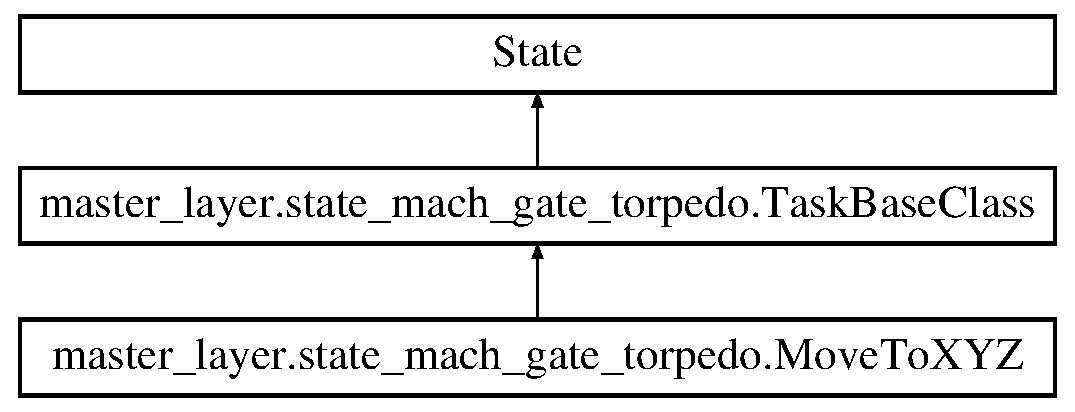
\includegraphics[height=3.000000cm]{classmaster__layer_1_1state__mach__gate__torpedo_1_1MoveToXYZ}
\end{center}
\end{figure}
\subsection*{Public Member Functions}
\begin{DoxyCompactItemize}
\item 
\mbox{\Hypertarget{classmaster__layer_1_1state__mach__gate__torpedo_1_1MoveToXYZ_a93923a104b3d70ded8df1652cc6f5d45}\label{classmaster__layer_1_1state__mach__gate__torpedo_1_1MoveToXYZ_a93923a104b3d70ded8df1652cc6f5d45}} 
def {\bfseries \+\_\+\+\_\+init\+\_\+\+\_\+} (self)
\item 
\mbox{\Hypertarget{classmaster__layer_1_1state__mach__gate__torpedo_1_1MoveToXYZ_a4f53a928896b9b3e2105e7d99cddeb4d}\label{classmaster__layer_1_1state__mach__gate__torpedo_1_1MoveToXYZ_a4f53a928896b9b3e2105e7d99cddeb4d}} 
def {\bfseries start\+\_\+moving} (self)
\item 
\mbox{\Hypertarget{classmaster__layer_1_1state__mach__gate__torpedo_1_1MoveToXYZ_a892f71e060bf7ea22b136ea8dabb2dc3}\label{classmaster__layer_1_1state__mach__gate__torpedo_1_1MoveToXYZ_a892f71e060bf7ea22b136ea8dabb2dc3}} 
def {\bfseries present\+\_\+status} (self)
\end{DoxyCompactItemize}
\subsection*{Public Attributes}
\begin{DoxyCompactItemize}
\item 
\mbox{\Hypertarget{classmaster__layer_1_1state__mach__gate__torpedo_1_1MoveToXYZ_a8e58005fcbde075fba55ba225bfba933}\label{classmaster__layer_1_1state__mach__gate__torpedo_1_1MoveToXYZ_a8e58005fcbde075fba55ba225bfba933}} 
{\bfseries then\+\_\+}
\item 
\mbox{\Hypertarget{classmaster__layer_1_1state__mach__gate__torpedo_1_1MoveToXYZ_a28a5c716de2c8d532a8842e79ef94721}\label{classmaster__layer_1_1state__mach__gate__torpedo_1_1MoveToXYZ_a28a5c716de2c8d532a8842e79ef94721}} 
{\bfseries timeout\+\_\+}
\item 
\mbox{\Hypertarget{classmaster__layer_1_1state__mach__gate__torpedo_1_1MoveToXYZ_a2c891d5bfdd04b183932c1ca0805bb61}\label{classmaster__layer_1_1state__mach__gate__torpedo_1_1MoveToXYZ_a2c891d5bfdd04b183932c1ca0805bb61}} 
{\bfseries target\+\_\+pose\+\_\+}
\end{DoxyCompactItemize}


The documentation for this class was generated from the following file\+:\begin{DoxyCompactItemize}
\item 
master\+\_\+layer/src/master\+\_\+layer/state\+\_\+mach\+\_\+gate\+\_\+torpedo.\+py\end{DoxyCompactItemize}

\hypertarget{classmaster__layer_1_1state__mach_1_1MoveToXYZ}{}\section{master\+\_\+layer.\+state\+\_\+mach.\+Move\+To\+X\+YZ Class Reference}
\label{classmaster__layer_1_1state__mach_1_1MoveToXYZ}\index{master\+\_\+layer.\+state\+\_\+mach.\+Move\+To\+X\+YZ@{master\+\_\+layer.\+state\+\_\+mach.\+Move\+To\+X\+YZ}}
Inheritance diagram for master\+\_\+layer.\+state\+\_\+mach.\+Move\+To\+X\+YZ\+:\begin{figure}[H]
\begin{center}
\leavevmode
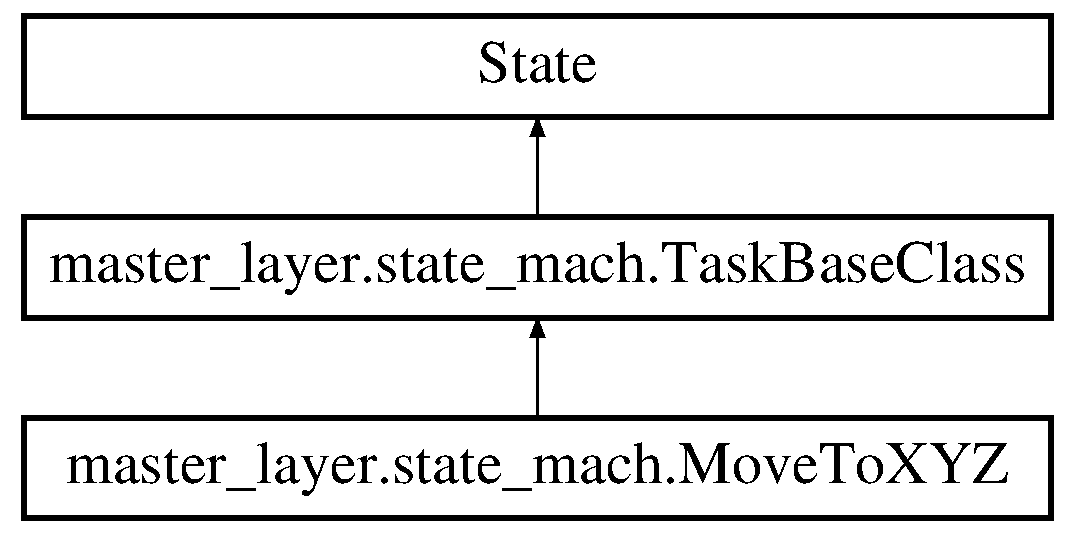
\includegraphics[height=3.000000cm]{classmaster__layer_1_1state__mach_1_1MoveToXYZ}
\end{center}
\end{figure}
\subsection*{Public Member Functions}
\begin{DoxyCompactItemize}
\item 
\mbox{\Hypertarget{classmaster__layer_1_1state__mach_1_1MoveToXYZ_adac823d47df44667b2094e59e67350d3}\label{classmaster__layer_1_1state__mach_1_1MoveToXYZ_adac823d47df44667b2094e59e67350d3}} 
def {\bfseries \+\_\+\+\_\+init\+\_\+\+\_\+} (self)
\item 
\mbox{\Hypertarget{classmaster__layer_1_1state__mach_1_1MoveToXYZ_a41cc58784894989aa81fba6c58e94715}\label{classmaster__layer_1_1state__mach_1_1MoveToXYZ_a41cc58784894989aa81fba6c58e94715}} 
def {\bfseries start\+\_\+moving} (self)
\item 
\mbox{\Hypertarget{classmaster__layer_1_1state__mach_1_1MoveToXYZ_a7645711937380d1ddae9516a21cb9d51}\label{classmaster__layer_1_1state__mach_1_1MoveToXYZ_a7645711937380d1ddae9516a21cb9d51}} 
def {\bfseries present\+\_\+status} (self)
\end{DoxyCompactItemize}
\subsection*{Public Attributes}
\begin{DoxyCompactItemize}
\item 
\mbox{\Hypertarget{classmaster__layer_1_1state__mach_1_1MoveToXYZ_a4ee2445296b2d7d9bbe9855a3d1b763d}\label{classmaster__layer_1_1state__mach_1_1MoveToXYZ_a4ee2445296b2d7d9bbe9855a3d1b763d}} 
{\bfseries then\+\_\+}
\item 
\mbox{\Hypertarget{classmaster__layer_1_1state__mach_1_1MoveToXYZ_ac93e574fe5fceb9f68f43da1ed1b5de4}\label{classmaster__layer_1_1state__mach_1_1MoveToXYZ_ac93e574fe5fceb9f68f43da1ed1b5de4}} 
{\bfseries timeout\+\_\+}
\item 
\mbox{\Hypertarget{classmaster__layer_1_1state__mach_1_1MoveToXYZ_a793e986622ff1433b868617f628dc268}\label{classmaster__layer_1_1state__mach_1_1MoveToXYZ_a793e986622ff1433b868617f628dc268}} 
{\bfseries target\+\_\+pose\+\_\+}
\end{DoxyCompactItemize}


The documentation for this class was generated from the following file\+:\begin{DoxyCompactItemize}
\item 
master\+\_\+layer/src/master\+\_\+layer/state\+\_\+mach.\+py\end{DoxyCompactItemize}

\hypertarget{classMS5837}{}\section{M\+S5837 Class Reference}
\label{classMS5837}\index{M\+S5837@{M\+S5837}}
\subsection*{Public Member Functions}
\begin{DoxyCompactItemize}
\item 
\mbox{\Hypertarget{classMS5837_accd5fa071ae977c796e4fb0648954499}\label{classMS5837_accd5fa071ae977c796e4fb0648954499}} 
bool {\bfseries init} ()
\item 
void \hyperlink{classMS5837_af8b0b1e168f39a9b99fa5918a6ef8f04}{set\+Model} (uint8\+\_\+t model)
\item 
void \hyperlink{classMS5837_a40ad0394fa84d49afa62ae63c411aa8f}{set\+Fluid\+Density} (float density)
\item 
void \hyperlink{classMS5837_a69b945b55b93c96173e8369fec1d9100}{read} ()
\item 
float \hyperlink{classMS5837_a14b4dd5598dc65e2d3f7c185e940af88}{pressure} (float conversion=1.\+0f)
\item 
float \hyperlink{classMS5837_a554d181ffc4329c1e292ca87e0a810f0}{temperature} ()
\item 
float \hyperlink{classMS5837_af5ec680e29a8cdaed429b9fb91d813e6}{depth} ()
\item 
float \hyperlink{classMS5837_af3c24ba068ed52a2918c784b3d608c8a}{altitude} ()
\end{DoxyCompactItemize}
\subsection*{Static Public Attributes}
\begin{DoxyCompactItemize}
\item 
\mbox{\Hypertarget{classMS5837_ae54d04a637682f68502e79d221bf00e3}\label{classMS5837_ae54d04a637682f68502e79d221bf00e3}} 
static const float {\bfseries Pa} = 100.\+0f
\item 
\mbox{\Hypertarget{classMS5837_afaf021ab4e8b402a642c383f35ff4258}\label{classMS5837_afaf021ab4e8b402a642c383f35ff4258}} 
static const float {\bfseries bar} = 0.\+001f
\item 
\mbox{\Hypertarget{classMS5837_a300724fab62674ab5e32a8b1861d3bba}\label{classMS5837_a300724fab62674ab5e32a8b1861d3bba}} 
static const float {\bfseries mbar} = 1.\+0f
\item 
\mbox{\Hypertarget{classMS5837_abc4a4367230b5ee53fbaf8060231a4bb}\label{classMS5837_abc4a4367230b5ee53fbaf8060231a4bb}} 
static const uint8\+\_\+t {\bfseries M\+S5837\+\_\+30\+BA} = 0
\item 
\mbox{\Hypertarget{classMS5837_a5b94f94735c695d94882f689fc55e853}\label{classMS5837_a5b94f94735c695d94882f689fc55e853}} 
static const uint8\+\_\+t {\bfseries M\+S5837\+\_\+02\+BA} = 1
\end{DoxyCompactItemize}


\subsection{Member Function Documentation}
\mbox{\Hypertarget{classMS5837_af3c24ba068ed52a2918c784b3d608c8a}\label{classMS5837_af3c24ba068ed52a2918c784b3d608c8a}} 
\index{M\+S5837@{M\+S5837}!altitude@{altitude}}
\index{altitude@{altitude}!M\+S5837@{M\+S5837}}
\subsubsection{\texorpdfstring{altitude()}{altitude()}}
{\footnotesize\ttfamily float M\+S5837\+::altitude (\begin{DoxyParamCaption}{ }\end{DoxyParamCaption})}

Altitude returned in meters (valid for operation in air only). \mbox{\Hypertarget{classMS5837_af5ec680e29a8cdaed429b9fb91d813e6}\label{classMS5837_af5ec680e29a8cdaed429b9fb91d813e6}} 
\index{M\+S5837@{M\+S5837}!depth@{depth}}
\index{depth@{depth}!M\+S5837@{M\+S5837}}
\subsubsection{\texorpdfstring{depth()}{depth()}}
{\footnotesize\ttfamily float M\+S5837\+::depth (\begin{DoxyParamCaption}{ }\end{DoxyParamCaption})}

Depth returned in meters (valid for operation in incompressible liquids only. Uses density that is set for fresh or seawater. \mbox{\Hypertarget{classMS5837_a14b4dd5598dc65e2d3f7c185e940af88}\label{classMS5837_a14b4dd5598dc65e2d3f7c185e940af88}} 
\index{M\+S5837@{M\+S5837}!pressure@{pressure}}
\index{pressure@{pressure}!M\+S5837@{M\+S5837}}
\subsubsection{\texorpdfstring{pressure()}{pressure()}}
{\footnotesize\ttfamily float M\+S5837\+::pressure (\begin{DoxyParamCaption}\item[{float}]{conversion = {\ttfamily 1.0f} }\end{DoxyParamCaption})}

Pressure returned in mbar or mbar$\ast$conversion rate. \mbox{\Hypertarget{classMS5837_a69b945b55b93c96173e8369fec1d9100}\label{classMS5837_a69b945b55b93c96173e8369fec1d9100}} 
\index{M\+S5837@{M\+S5837}!read@{read}}
\index{read@{read}!M\+S5837@{M\+S5837}}
\subsubsection{\texorpdfstring{read()}{read()}}
{\footnotesize\ttfamily void M\+S5837\+::read (\begin{DoxyParamCaption}{ }\end{DoxyParamCaption})}

The read from I2C takes up to 40 ms, so use sparingly is possible. \mbox{\Hypertarget{classMS5837_a40ad0394fa84d49afa62ae63c411aa8f}\label{classMS5837_a40ad0394fa84d49afa62ae63c411aa8f}} 
\index{M\+S5837@{M\+S5837}!set\+Fluid\+Density@{set\+Fluid\+Density}}
\index{set\+Fluid\+Density@{set\+Fluid\+Density}!M\+S5837@{M\+S5837}}
\subsubsection{\texorpdfstring{set\+Fluid\+Density()}{setFluidDensity()}}
{\footnotesize\ttfamily void M\+S5837\+::set\+Fluid\+Density (\begin{DoxyParamCaption}\item[{float}]{density }\end{DoxyParamCaption})}

Provide the density of the working fluid in kg/m$^\wedge$3. Default is for seawater. Should be 997 for freshwater. \mbox{\Hypertarget{classMS5837_af8b0b1e168f39a9b99fa5918a6ef8f04}\label{classMS5837_af8b0b1e168f39a9b99fa5918a6ef8f04}} 
\index{M\+S5837@{M\+S5837}!set\+Model@{set\+Model}}
\index{set\+Model@{set\+Model}!M\+S5837@{M\+S5837}}
\subsubsection{\texorpdfstring{set\+Model()}{setModel()}}
{\footnotesize\ttfamily void M\+S5837\+::set\+Model (\begin{DoxyParamCaption}\item[{uint8\+\_\+t}]{model }\end{DoxyParamCaption})}

Set model of \hyperlink{classMS5837}{M\+S5837} sensor. Valid options are M\+S5837\+::\+M\+S5837\+\_\+30\+BA (default) and M\+S5837\+::\+M\+S5837\+\_\+02\+BA. \mbox{\Hypertarget{classMS5837_a554d181ffc4329c1e292ca87e0a810f0}\label{classMS5837_a554d181ffc4329c1e292ca87e0a810f0}} 
\index{M\+S5837@{M\+S5837}!temperature@{temperature}}
\index{temperature@{temperature}!M\+S5837@{M\+S5837}}
\subsubsection{\texorpdfstring{temperature()}{temperature()}}
{\footnotesize\ttfamily float M\+S5837\+::temperature (\begin{DoxyParamCaption}{ }\end{DoxyParamCaption})}

Temperature returned in deg C. 

The documentation for this class was generated from the following files\+:\begin{DoxyCompactItemize}
\item 
hardware\+\_\+layer/hardware\+\_\+arduino/include/M\+S5837.\+h\item 
hardware\+\_\+layer/hardware\+\_\+arduino/src/M\+S5837.\+cpp\end{DoxyCompactItemize}

\hypertarget{classmtdevice_1_1MTDevice}{}\doxysection{mtdevice.\+M\+T\+Device Class Reference}
\label{classmtdevice_1_1MTDevice}\index{mtdevice.MTDevice@{mtdevice.MTDevice}}


\mbox{\hyperlink{classmtdevice_1_1MTDevice}{M\+T\+Device}} class.  


Inheritance diagram for mtdevice.\+M\+T\+Device\+:\begin{figure}[H]
\begin{center}
\leavevmode
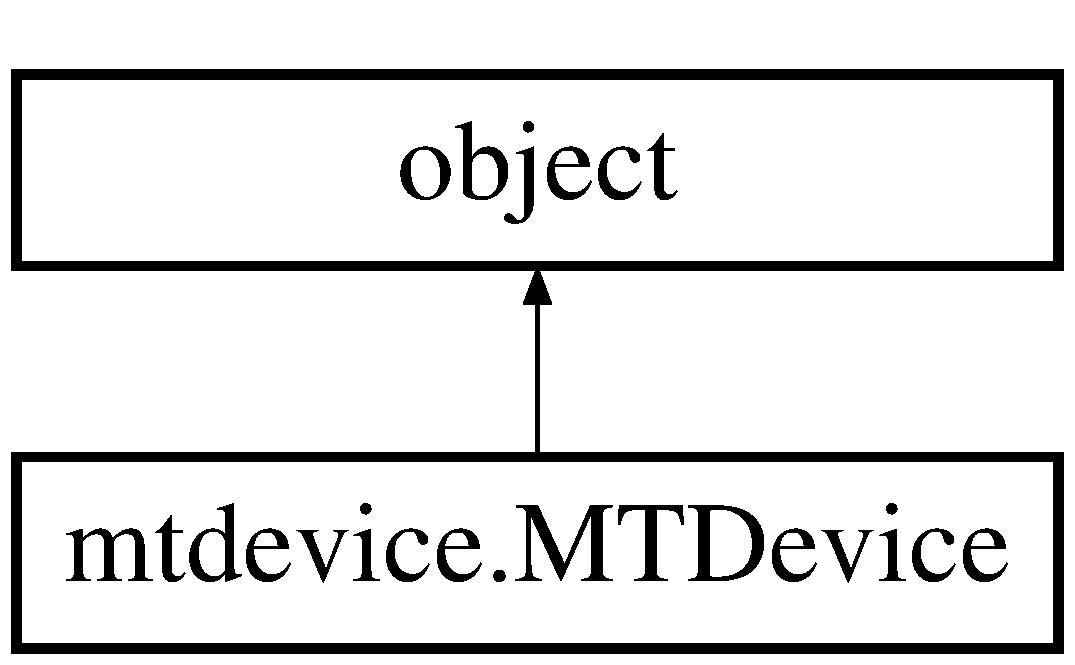
\includegraphics[height=2.000000cm]{classmtdevice_1_1MTDevice}
\end{center}
\end{figure}
\doxysubsection*{Public Member Functions}
\begin{DoxyCompactItemize}
\item 
def \mbox{\hyperlink{classmtdevice_1_1MTDevice_a9a93b603a3c9ab6a7ad9027e436799d4}{\+\_\+\+\_\+init\+\_\+\+\_\+}} (self, port, baudrate=115200, timeout=0.\+002, autoconf=True, config\+\_\+mode=False, verbose=False, initial\+\_\+wait=0.\+1)
\item 
def \mbox{\hyperlink{classmtdevice_1_1MTDevice_a8b4e4d222ab28dd708a4ecc220af343c}{write\+\_\+msg}} (self, mid, data=b\textquotesingle{}\textquotesingle{})
\begin{DoxyCompactList}\small\item\em Low-\/level communication. \end{DoxyCompactList}\item 
def \mbox{\hyperlink{classmtdevice_1_1MTDevice_a072aad4573d20a44ac7d18fcbf985546}{waitfor}} (self, size=1)
\item 
def \mbox{\hyperlink{classmtdevice_1_1MTDevice_a86a979700d1d0f891943e7275d470f1f}{read\+\_\+data\+\_\+msg}} (self, buf=bytearray())
\item 
def \mbox{\hyperlink{classmtdevice_1_1MTDevice_ac5598d36cd10ab80e28d41c60281addd}{read\+\_\+msg}} (self)
\item 
def \mbox{\hyperlink{classmtdevice_1_1MTDevice_aecbd2a94d3e4b6dd67193549d3668d2f}{write\+\_\+ack}} (self, mid, data=b\textquotesingle{}\textquotesingle{}, n\+\_\+retries=500)
\item 
def \mbox{\hyperlink{classmtdevice_1_1MTDevice_aa3a48c919b8a17d421468faba4b7045f}{Reset}} (self, go\+\_\+to\+\_\+config=False)
\begin{DoxyCompactList}\small\item\em High-\/level functions. \end{DoxyCompactList}\item 
def \mbox{\hyperlink{classmtdevice_1_1MTDevice_a61464532dbf30f237794801053ef89e1}{Go\+To\+Config}} (self)
\item 
def \mbox{\hyperlink{classmtdevice_1_1MTDevice_ab6e5df72a835897e8e376e574e07376e}{Go\+To\+Measurement}} (self)
\item 
def \mbox{\hyperlink{classmtdevice_1_1MTDevice_aa634cb80bc49f34e4a41fd9214f20d9a}{Get\+Device\+ID}} (self)
\item 
def \mbox{\hyperlink{classmtdevice_1_1MTDevice_a80f12839fe7f3ebe2e94a8c21641f2ae}{Get\+Product\+Code}} (self)
\item 
def \mbox{\hyperlink{classmtdevice_1_1MTDevice_a1f31e322a4232994ac49fb641f3d3cc0}{Get\+Firmware\+Rev}} (self)
\item 
def \mbox{\hyperlink{classmtdevice_1_1MTDevice_a259fb7d60c601ebe00e539c9a96ec9f7}{Run\+Self\+Test}} (self)
\item 
def \mbox{\hyperlink{classmtdevice_1_1MTDevice_a815cba09b30c67bec0c1405dc916cf96}{Get\+Baudrate}} (self)
\item 
def \mbox{\hyperlink{classmtdevice_1_1MTDevice_ac964b061548751f4885b12dc01a0a0f7}{Set\+Baudrate}} (self, brid)
\item 
def \mbox{\hyperlink{classmtdevice_1_1MTDevice_af7939b8d550d4016f3078a5e8ea80020}{Get\+Error\+Mode}} (self)
\item 
def \mbox{\hyperlink{classmtdevice_1_1MTDevice_a9f8b2a581a49333421f371ea1403b953}{Set\+Error\+Mode}} (self, error\+\_\+mode)
\item 
def \mbox{\hyperlink{classmtdevice_1_1MTDevice_ad4de7b6d2e4e8e033e2ac7f998554537}{Get\+Option\+Flags}} (self)
\item 
def \mbox{\hyperlink{classmtdevice_1_1MTDevice_adf0f4d946d65c78dcf641d9b7dd2c9e0}{Set\+Option\+Flags}} (self, set\+\_\+flags, clear\+\_\+flags)
\item 
def \mbox{\hyperlink{classmtdevice_1_1MTDevice_abc9c9bc4f9e83745b2d34df960050efa}{Get\+Location\+ID}} (self)
\item 
def \mbox{\hyperlink{classmtdevice_1_1MTDevice_a82701d9577a6bf7323b9a5649bebe4e0}{Set\+Location\+ID}} (self, location\+\_\+id)
\item 
def \mbox{\hyperlink{classmtdevice_1_1MTDevice_a1b86412ad2c180bcfd6bbf4ea62f76a4}{Restore\+Factory\+Defaults}} (self)
\item 
def \mbox{\hyperlink{classmtdevice_1_1MTDevice_a7e0df33d903e96c8beaf7f136075cff1}{Get\+Transmit\+Delay}} (self)
\item 
def \mbox{\hyperlink{classmtdevice_1_1MTDevice_a439b399cd20ca95cfad6225f368651f2}{Set\+Transmit\+Delay}} (self, transmit\+\_\+delay)
\item 
def \mbox{\hyperlink{classmtdevice_1_1MTDevice_af518193ff364835d40017be2a0fdde45}{Get\+Sync\+Settings}} (self)
\item 
def \mbox{\hyperlink{classmtdevice_1_1MTDevice_a339cd8bc34b6fa9c1f4dc7b8c8751576}{Set\+Sync\+Settings}} (self, sync\+\_\+settings)
\item 
def \mbox{\hyperlink{classmtdevice_1_1MTDevice_a2d75ac2afb3feded6ca6ac0fabb54aef}{Get\+Configuration}} (self)
\item 
def \mbox{\hyperlink{classmtdevice_1_1MTDevice_a14e52089e2cc376e2ac1c77283a348d1}{Get\+Output\+Configuration}} (self)
\item 
def \mbox{\hyperlink{classmtdevice_1_1MTDevice_a53c95416ed262990d70b667497a44d71}{Set\+Output\+Configuration}} (self, output\+\_\+configuration)
\item 
def \mbox{\hyperlink{classmtdevice_1_1MTDevice_ab265cda5a90f2089720c4028a6d64d45}{Get\+String\+Output\+Type}} (self)
\item 
def \mbox{\hyperlink{classmtdevice_1_1MTDevice_a7ef3bdc62f343cb2ba1b7b497c83cda3}{Set\+String\+Output\+Type}} (self, string\+\_\+output\+\_\+type)
\item 
def \mbox{\hyperlink{classmtdevice_1_1MTDevice_a9964a8f360efe414c9bd84d173cff963}{Get\+Period}} (self)
\item 
def \mbox{\hyperlink{classmtdevice_1_1MTDevice_a7421eafc5d4d03fc6e7d419dd5d687e4}{Set\+Period}} (self, period)
\item 
def \mbox{\hyperlink{classmtdevice_1_1MTDevice_a4473bb21765c708b18803fc26d8cc4d2}{Get\+Alignment\+Rotation}} (self, parameter)
\item 
def \mbox{\hyperlink{classmtdevice_1_1MTDevice_ad7f11554fdb3d2ce24d2ca081ca972c6}{Set\+Alignment\+Rotation}} (self, parameter, quaternion)
\item 
def \mbox{\hyperlink{classmtdevice_1_1MTDevice_af193eb2f64536239389fb4ba83a21d86}{Get\+Output\+Mode}} (self)
\item 
def \mbox{\hyperlink{classmtdevice_1_1MTDevice_a1e990d315750492fa1afbd49990959cc}{Set\+Output\+Mode}} (self, mode)
\item 
def \mbox{\hyperlink{classmtdevice_1_1MTDevice_a66e75cf601b0a7cfef3f456300d7520d}{Get\+Ext\+Output\+Mode}} (self)
\item 
def \mbox{\hyperlink{classmtdevice_1_1MTDevice_a5cd787accdbf2aec47fc0edf2835df40}{Set\+Ext\+Output\+Mode}} (self, ext\+\_\+mode)
\item 
def \mbox{\hyperlink{classmtdevice_1_1MTDevice_a782fd0b3a63007569b8c009ae7c1d8cc}{Get\+Output\+Settings}} (self)
\item 
def \mbox{\hyperlink{classmtdevice_1_1MTDevice_ac8f77a2d1d393aea71a7790929791cc0}{Set\+Output\+Settings}} (self, settings)
\item 
def \mbox{\hyperlink{classmtdevice_1_1MTDevice_a00ae63328881e07081d07a385ecfe858}{Set\+Output\+Skip\+Factor}} (self, skipfactor)
\item 
def \mbox{\hyperlink{classmtdevice_1_1MTDevice_a948beab4131a0748c8943d5abce96394}{Req\+Data\+Length}} (self)
\item 
def \mbox{\hyperlink{classmtdevice_1_1MTDevice_a80fa3cd0b6bf97a2ba46771e891d3fd1}{Get\+Lat\+Lon\+Alt}} (self)
\item 
def \mbox{\hyperlink{classmtdevice_1_1MTDevice_adb65653ac4a1509c3fbd9122b63365da}{Set\+Lat\+Lon\+Alt}} (self, lat, lon, alt)
\item 
def \mbox{\hyperlink{classmtdevice_1_1MTDevice_ad55a649988c828b49bc2af507c39da93}{Get\+Available\+Scenarios}} (self)
\item 
def \mbox{\hyperlink{classmtdevice_1_1MTDevice_ac63944270e1c85c2c4c9fcc500474ab5}{Get\+Current\+Scenario}} (self)
\item 
def \mbox{\hyperlink{classmtdevice_1_1MTDevice_a94eaa1bb8de52ed69bb20c9ffa404fe8}{Set\+Current\+Scenario}} (self, scenario\+\_\+id)
\item 
def \mbox{\hyperlink{classmtdevice_1_1MTDevice_a29424b8cc73d27252ed151075735c0e5}{Reset\+Orientation}} (self, code)
\item 
def \mbox{\hyperlink{classmtdevice_1_1MTDevice_aec52bfabf3122d033b56d7e596d3c036}{Set\+No\+Rotation}} (self, duration)
\item 
def \mbox{\hyperlink{classmtdevice_1_1MTDevice_aa5a60e82059880b43492ea174ac36d6c}{Get\+U\+T\+C\+Time}} (self)
\item 
def \mbox{\hyperlink{classmtdevice_1_1MTDevice_a8e431e7cfdf17e72d9bdc1eddcf80d43}{Set\+U\+T\+C\+Time}} (self, ns, year, month, day, hour, minute, second, flag)
\item 
def \mbox{\hyperlink{classmtdevice_1_1MTDevice_af18ecf9cbdca13076b655a6b83f8fab2}{Adjust\+U\+T\+C\+Time}} (self, ticks)
\item 
def \mbox{\hyperlink{classmtdevice_1_1MTDevice_a487b8703cde676cd0877e0b07a40ed0c}{configure\+\_\+legacy}} (self, mode, settings, period=None, skipfactor=None)
\begin{DoxyCompactList}\small\item\em High-\/level utility functions. \end{DoxyCompactList}\item 
def \mbox{\hyperlink{classmtdevice_1_1MTDevice_a2f6e1f0e3ca9c5459b97dc1007050c7b}{auto\+\_\+config\+\_\+legacy}} (self)
\item 
\mbox{\Hypertarget{classmtdevice_1_1MTDevice_ac8b5e65c0dbc76a21ce0d783fad0e622}\label{classmtdevice_1_1MTDevice_ac8b5e65c0dbc76a21ce0d783fad0e622}} 
def {\bfseries read\+\_\+measurement} (self, mode=None, settings=None)
\item 
\mbox{\Hypertarget{classmtdevice_1_1MTDevice_a6e34005b0463c21c75ddc0986600d36d}\label{classmtdevice_1_1MTDevice_a6e34005b0463c21c75ddc0986600d36d}} 
def {\bfseries parse\+\_\+\+M\+T\+Data2} (self, data)
\item 
def \mbox{\hyperlink{classmtdevice_1_1MTDevice_a797870c42c7c882a20806279dc984355}{parse\+\_\+\+M\+T\+Data}} (self, data, mode=None, settings=None)
\item 
def \mbox{\hyperlink{classmtdevice_1_1MTDevice_a065580ecd5e3906b8f49c46c1b1510e7}{Change\+Baudrate}} (self, baudrate)
\end{DoxyCompactItemize}
\doxysubsection*{Public Attributes}
\begin{DoxyCompactItemize}
\item 
\mbox{\Hypertarget{classmtdevice_1_1MTDevice_a6dcc0bc56086e927423db95656856d10}\label{classmtdevice_1_1MTDevice_a6dcc0bc56086e927423db95656856d10}} 
{\bfseries verbose}
\item 
\mbox{\Hypertarget{classmtdevice_1_1MTDevice_af9445fdb0f702410f2bf23d69c92efa5}\label{classmtdevice_1_1MTDevice_af9445fdb0f702410f2bf23d69c92efa5}} 
{\bfseries device}
\item 
\mbox{\Hypertarget{classmtdevice_1_1MTDevice_a91c1ae6fa1d5d15044bba922e42ceafb}\label{classmtdevice_1_1MTDevice_a91c1ae6fa1d5d15044bba922e42ceafb}} 
{\bfseries timeout}
\item 
\mbox{\Hypertarget{classmtdevice_1_1MTDevice_ac50a29b63d176b4261060d50d1758e32}\label{classmtdevice_1_1MTDevice_ac50a29b63d176b4261060d50d1758e32}} 
{\bfseries state}
\item 
\mbox{\Hypertarget{classmtdevice_1_1MTDevice_ab24f4baabcc6525727f9f4c5dee1e226}\label{classmtdevice_1_1MTDevice_ab24f4baabcc6525727f9f4c5dee1e226}} 
{\bfseries mode}
\item 
\mbox{\Hypertarget{classmtdevice_1_1MTDevice_a11283b18b5ced9424dc73efe03a49fd8}\label{classmtdevice_1_1MTDevice_a11283b18b5ced9424dc73efe03a49fd8}} 
{\bfseries settings}
\item 
\mbox{\Hypertarget{classmtdevice_1_1MTDevice_a9b8218f5a01b92e698ac428ea481c948}\label{classmtdevice_1_1MTDevice_a9b8218f5a01b92e698ac428ea481c948}} 
{\bfseries length}
\item 
\mbox{\Hypertarget{classmtdevice_1_1MTDevice_aeced4192f195e40e5c3d2bee968f0fd7}\label{classmtdevice_1_1MTDevice_aeced4192f195e40e5c3d2bee968f0fd7}} 
{\bfseries header}
\item 
\mbox{\Hypertarget{classmtdevice_1_1MTDevice_a194a8ba29c60bf12b87b5927b0aed098}\label{classmtdevice_1_1MTDevice_a194a8ba29c60bf12b87b5927b0aed098}} 
{\bfseries scenarios}
\item 
\mbox{\Hypertarget{classmtdevice_1_1MTDevice_a4bab15bccdddcdf12e08c34926b2c03c}\label{classmtdevice_1_1MTDevice_a4bab15bccdddcdf12e08c34926b2c03c}} 
{\bfseries scenario\+\_\+id}
\end{DoxyCompactItemize}


\doxysubsection{Detailed Description}
\mbox{\hyperlink{classmtdevice_1_1MTDevice}{M\+T\+Device}} class. 

\begin{DoxyVerb}XSens MT device communication object.\end{DoxyVerb}
 

\doxysubsection{Constructor \& Destructor Documentation}
\mbox{\Hypertarget{classmtdevice_1_1MTDevice_a9a93b603a3c9ab6a7ad9027e436799d4}\label{classmtdevice_1_1MTDevice_a9a93b603a3c9ab6a7ad9027e436799d4}} 
\index{mtdevice.MTDevice@{mtdevice.MTDevice}!\_\_init\_\_@{\_\_init\_\_}}
\index{\_\_init\_\_@{\_\_init\_\_}!mtdevice.MTDevice@{mtdevice.MTDevice}}
\doxysubsubsection{\texorpdfstring{\_\_init\_\_()}{\_\_init\_\_()}}
{\footnotesize\ttfamily def mtdevice.\+M\+T\+Device.\+\_\+\+\_\+init\+\_\+\+\_\+ (\begin{DoxyParamCaption}\item[{}]{self,  }\item[{}]{port,  }\item[{}]{baudrate = {\ttfamily 115200},  }\item[{}]{timeout = {\ttfamily 0.002},  }\item[{}]{autoconf = {\ttfamily True},  }\item[{}]{config\+\_\+mode = {\ttfamily False},  }\item[{}]{verbose = {\ttfamily False},  }\item[{}]{initial\+\_\+wait = {\ttfamily 0.1} }\end{DoxyParamCaption})}

\begin{DoxyVerb}Open device.\end{DoxyVerb}
 

\doxysubsection{Member Function Documentation}
\mbox{\Hypertarget{classmtdevice_1_1MTDevice_af18ecf9cbdca13076b655a6b83f8fab2}\label{classmtdevice_1_1MTDevice_af18ecf9cbdca13076b655a6b83f8fab2}} 
\index{mtdevice.MTDevice@{mtdevice.MTDevice}!AdjustUTCTime@{AdjustUTCTime}}
\index{AdjustUTCTime@{AdjustUTCTime}!mtdevice.MTDevice@{mtdevice.MTDevice}}
\doxysubsubsection{\texorpdfstring{AdjustUTCTime()}{AdjustUTCTime()}}
{\footnotesize\ttfamily def mtdevice.\+M\+T\+Device.\+Adjust\+U\+T\+C\+Time (\begin{DoxyParamCaption}\item[{}]{self,  }\item[{}]{ticks }\end{DoxyParamCaption})}

\begin{DoxyVerb}Adjust UTC Time of device using correction ticks (0.1 ms).\end{DoxyVerb}
 \mbox{\Hypertarget{classmtdevice_1_1MTDevice_a2f6e1f0e3ca9c5459b97dc1007050c7b}\label{classmtdevice_1_1MTDevice_a2f6e1f0e3ca9c5459b97dc1007050c7b}} 
\index{mtdevice.MTDevice@{mtdevice.MTDevice}!auto\_config\_legacy@{auto\_config\_legacy}}
\index{auto\_config\_legacy@{auto\_config\_legacy}!mtdevice.MTDevice@{mtdevice.MTDevice}}
\doxysubsubsection{\texorpdfstring{auto\_config\_legacy()}{auto\_config\_legacy()}}
{\footnotesize\ttfamily def mtdevice.\+M\+T\+Device.\+auto\+\_\+config\+\_\+legacy (\begin{DoxyParamCaption}\item[{}]{self }\end{DoxyParamCaption})}

\begin{DoxyVerb}Read configuration from device in legacy mode.\end{DoxyVerb}
 \mbox{\Hypertarget{classmtdevice_1_1MTDevice_a065580ecd5e3906b8f49c46c1b1510e7}\label{classmtdevice_1_1MTDevice_a065580ecd5e3906b8f49c46c1b1510e7}} 
\index{mtdevice.MTDevice@{mtdevice.MTDevice}!ChangeBaudrate@{ChangeBaudrate}}
\index{ChangeBaudrate@{ChangeBaudrate}!mtdevice.MTDevice@{mtdevice.MTDevice}}
\doxysubsubsection{\texorpdfstring{ChangeBaudrate()}{ChangeBaudrate()}}
{\footnotesize\ttfamily def mtdevice.\+M\+T\+Device.\+Change\+Baudrate (\begin{DoxyParamCaption}\item[{}]{self,  }\item[{}]{baudrate }\end{DoxyParamCaption})}

\begin{DoxyVerb}Change the baudrate, reset the device and reopen communication.\end{DoxyVerb}
 \mbox{\Hypertarget{classmtdevice_1_1MTDevice_a487b8703cde676cd0877e0b07a40ed0c}\label{classmtdevice_1_1MTDevice_a487b8703cde676cd0877e0b07a40ed0c}} 
\index{mtdevice.MTDevice@{mtdevice.MTDevice}!configure\_legacy@{configure\_legacy}}
\index{configure\_legacy@{configure\_legacy}!mtdevice.MTDevice@{mtdevice.MTDevice}}
\doxysubsubsection{\texorpdfstring{configure\_legacy()}{configure\_legacy()}}
{\footnotesize\ttfamily def mtdevice.\+M\+T\+Device.\+configure\+\_\+legacy (\begin{DoxyParamCaption}\item[{}]{self,  }\item[{}]{mode,  }\item[{}]{settings,  }\item[{}]{period = {\ttfamily None},  }\item[{}]{skipfactor = {\ttfamily None} }\end{DoxyParamCaption})}



High-\/level utility functions. 

\begin{DoxyVerb}Configure the mode and settings of the MT device in legacy mode.\end{DoxyVerb}
 \mbox{\Hypertarget{classmtdevice_1_1MTDevice_a4473bb21765c708b18803fc26d8cc4d2}\label{classmtdevice_1_1MTDevice_a4473bb21765c708b18803fc26d8cc4d2}} 
\index{mtdevice.MTDevice@{mtdevice.MTDevice}!GetAlignmentRotation@{GetAlignmentRotation}}
\index{GetAlignmentRotation@{GetAlignmentRotation}!mtdevice.MTDevice@{mtdevice.MTDevice}}
\doxysubsubsection{\texorpdfstring{GetAlignmentRotation()}{GetAlignmentRotation()}}
{\footnotesize\ttfamily def mtdevice.\+M\+T\+Device.\+Get\+Alignment\+Rotation (\begin{DoxyParamCaption}\item[{}]{self,  }\item[{}]{parameter }\end{DoxyParamCaption})}

\begin{DoxyVerb}Get the object alignment.

parameter indicates the desired alignment quaternion:
    0 for sensor alignment (RotSensor),
    1 for local alignment (RotLocal).
\end{DoxyVerb}
 \mbox{\Hypertarget{classmtdevice_1_1MTDevice_ad55a649988c828b49bc2af507c39da93}\label{classmtdevice_1_1MTDevice_ad55a649988c828b49bc2af507c39da93}} 
\index{mtdevice.MTDevice@{mtdevice.MTDevice}!GetAvailableScenarios@{GetAvailableScenarios}}
\index{GetAvailableScenarios@{GetAvailableScenarios}!mtdevice.MTDevice@{mtdevice.MTDevice}}
\doxysubsubsection{\texorpdfstring{GetAvailableScenarios()}{GetAvailableScenarios()}}
{\footnotesize\ttfamily def mtdevice.\+M\+T\+Device.\+Get\+Available\+Scenarios (\begin{DoxyParamCaption}\item[{}]{self }\end{DoxyParamCaption})}

\begin{DoxyVerb}Get the available XKF scenarios on the device.\end{DoxyVerb}
 \mbox{\Hypertarget{classmtdevice_1_1MTDevice_a815cba09b30c67bec0c1405dc916cf96}\label{classmtdevice_1_1MTDevice_a815cba09b30c67bec0c1405dc916cf96}} 
\index{mtdevice.MTDevice@{mtdevice.MTDevice}!GetBaudrate@{GetBaudrate}}
\index{GetBaudrate@{GetBaudrate}!mtdevice.MTDevice@{mtdevice.MTDevice}}
\doxysubsubsection{\texorpdfstring{GetBaudrate()}{GetBaudrate()}}
{\footnotesize\ttfamily def mtdevice.\+M\+T\+Device.\+Get\+Baudrate (\begin{DoxyParamCaption}\item[{}]{self }\end{DoxyParamCaption})}

\begin{DoxyVerb}Get the current baudrate id of the device.\end{DoxyVerb}
 \mbox{\Hypertarget{classmtdevice_1_1MTDevice_a2d75ac2afb3feded6ca6ac0fabb54aef}\label{classmtdevice_1_1MTDevice_a2d75ac2afb3feded6ca6ac0fabb54aef}} 
\index{mtdevice.MTDevice@{mtdevice.MTDevice}!GetConfiguration@{GetConfiguration}}
\index{GetConfiguration@{GetConfiguration}!mtdevice.MTDevice@{mtdevice.MTDevice}}
\doxysubsubsection{\texorpdfstring{GetConfiguration()}{GetConfiguration()}}
{\footnotesize\ttfamily def mtdevice.\+M\+T\+Device.\+Get\+Configuration (\begin{DoxyParamCaption}\item[{}]{self }\end{DoxyParamCaption})}

\begin{DoxyVerb}Ask for the current configuration of the MT device.\end{DoxyVerb}
 \mbox{\Hypertarget{classmtdevice_1_1MTDevice_ac63944270e1c85c2c4c9fcc500474ab5}\label{classmtdevice_1_1MTDevice_ac63944270e1c85c2c4c9fcc500474ab5}} 
\index{mtdevice.MTDevice@{mtdevice.MTDevice}!GetCurrentScenario@{GetCurrentScenario}}
\index{GetCurrentScenario@{GetCurrentScenario}!mtdevice.MTDevice@{mtdevice.MTDevice}}
\doxysubsubsection{\texorpdfstring{GetCurrentScenario()}{GetCurrentScenario()}}
{\footnotesize\ttfamily def mtdevice.\+M\+T\+Device.\+Get\+Current\+Scenario (\begin{DoxyParamCaption}\item[{}]{self }\end{DoxyParamCaption})}

\begin{DoxyVerb}Get the ID of the currently used XKF scenario.\end{DoxyVerb}
 \mbox{\Hypertarget{classmtdevice_1_1MTDevice_aa634cb80bc49f34e4a41fd9214f20d9a}\label{classmtdevice_1_1MTDevice_aa634cb80bc49f34e4a41fd9214f20d9a}} 
\index{mtdevice.MTDevice@{mtdevice.MTDevice}!GetDeviceID@{GetDeviceID}}
\index{GetDeviceID@{GetDeviceID}!mtdevice.MTDevice@{mtdevice.MTDevice}}
\doxysubsubsection{\texorpdfstring{GetDeviceID()}{GetDeviceID()}}
{\footnotesize\ttfamily def mtdevice.\+M\+T\+Device.\+Get\+Device\+ID (\begin{DoxyParamCaption}\item[{}]{self }\end{DoxyParamCaption})}

\begin{DoxyVerb}Get the device identifier.\end{DoxyVerb}
 \mbox{\Hypertarget{classmtdevice_1_1MTDevice_af7939b8d550d4016f3078a5e8ea80020}\label{classmtdevice_1_1MTDevice_af7939b8d550d4016f3078a5e8ea80020}} 
\index{mtdevice.MTDevice@{mtdevice.MTDevice}!GetErrorMode@{GetErrorMode}}
\index{GetErrorMode@{GetErrorMode}!mtdevice.MTDevice@{mtdevice.MTDevice}}
\doxysubsubsection{\texorpdfstring{GetErrorMode()}{GetErrorMode()}}
{\footnotesize\ttfamily def mtdevice.\+M\+T\+Device.\+Get\+Error\+Mode (\begin{DoxyParamCaption}\item[{}]{self }\end{DoxyParamCaption})}

\begin{DoxyVerb}Get the current error mode of the device.\end{DoxyVerb}
 \mbox{\Hypertarget{classmtdevice_1_1MTDevice_a66e75cf601b0a7cfef3f456300d7520d}\label{classmtdevice_1_1MTDevice_a66e75cf601b0a7cfef3f456300d7520d}} 
\index{mtdevice.MTDevice@{mtdevice.MTDevice}!GetExtOutputMode@{GetExtOutputMode}}
\index{GetExtOutputMode@{GetExtOutputMode}!mtdevice.MTDevice@{mtdevice.MTDevice}}
\doxysubsubsection{\texorpdfstring{GetExtOutputMode()}{GetExtOutputMode()}}
{\footnotesize\ttfamily def mtdevice.\+M\+T\+Device.\+Get\+Ext\+Output\+Mode (\begin{DoxyParamCaption}\item[{}]{self }\end{DoxyParamCaption})}

\begin{DoxyVerb}Get current extended output mode (for alternative UART).\end{DoxyVerb}
 \mbox{\Hypertarget{classmtdevice_1_1MTDevice_a1f31e322a4232994ac49fb641f3d3cc0}\label{classmtdevice_1_1MTDevice_a1f31e322a4232994ac49fb641f3d3cc0}} 
\index{mtdevice.MTDevice@{mtdevice.MTDevice}!GetFirmwareRev@{GetFirmwareRev}}
\index{GetFirmwareRev@{GetFirmwareRev}!mtdevice.MTDevice@{mtdevice.MTDevice}}
\doxysubsubsection{\texorpdfstring{GetFirmwareRev()}{GetFirmwareRev()}}
{\footnotesize\ttfamily def mtdevice.\+M\+T\+Device.\+Get\+Firmware\+Rev (\begin{DoxyParamCaption}\item[{}]{self }\end{DoxyParamCaption})}

\begin{DoxyVerb}Get the firmware version.\end{DoxyVerb}
 \mbox{\Hypertarget{classmtdevice_1_1MTDevice_a80fa3cd0b6bf97a2ba46771e891d3fd1}\label{classmtdevice_1_1MTDevice_a80fa3cd0b6bf97a2ba46771e891d3fd1}} 
\index{mtdevice.MTDevice@{mtdevice.MTDevice}!GetLatLonAlt@{GetLatLonAlt}}
\index{GetLatLonAlt@{GetLatLonAlt}!mtdevice.MTDevice@{mtdevice.MTDevice}}
\doxysubsubsection{\texorpdfstring{GetLatLonAlt()}{GetLatLonAlt()}}
{\footnotesize\ttfamily def mtdevice.\+M\+T\+Device.\+Get\+Lat\+Lon\+Alt (\begin{DoxyParamCaption}\item[{}]{self }\end{DoxyParamCaption})}

\begin{DoxyVerb}Get the stored position of the device.
It is used internally for local magnetic declination and local gravity.
\end{DoxyVerb}
 \mbox{\Hypertarget{classmtdevice_1_1MTDevice_abc9c9bc4f9e83745b2d34df960050efa}\label{classmtdevice_1_1MTDevice_abc9c9bc4f9e83745b2d34df960050efa}} 
\index{mtdevice.MTDevice@{mtdevice.MTDevice}!GetLocationID@{GetLocationID}}
\index{GetLocationID@{GetLocationID}!mtdevice.MTDevice@{mtdevice.MTDevice}}
\doxysubsubsection{\texorpdfstring{GetLocationID()}{GetLocationID()}}
{\footnotesize\ttfamily def mtdevice.\+M\+T\+Device.\+Get\+Location\+ID (\begin{DoxyParamCaption}\item[{}]{self }\end{DoxyParamCaption})}

\begin{DoxyVerb}Get the location ID of the device.\end{DoxyVerb}
 \mbox{\Hypertarget{classmtdevice_1_1MTDevice_ad4de7b6d2e4e8e033e2ac7f998554537}\label{classmtdevice_1_1MTDevice_ad4de7b6d2e4e8e033e2ac7f998554537}} 
\index{mtdevice.MTDevice@{mtdevice.MTDevice}!GetOptionFlags@{GetOptionFlags}}
\index{GetOptionFlags@{GetOptionFlags}!mtdevice.MTDevice@{mtdevice.MTDevice}}
\doxysubsubsection{\texorpdfstring{GetOptionFlags()}{GetOptionFlags()}}
{\footnotesize\ttfamily def mtdevice.\+M\+T\+Device.\+Get\+Option\+Flags (\begin{DoxyParamCaption}\item[{}]{self }\end{DoxyParamCaption})}

\begin{DoxyVerb}Get the option flags (MTi-1 series).\end{DoxyVerb}
 \mbox{\Hypertarget{classmtdevice_1_1MTDevice_a14e52089e2cc376e2ac1c77283a348d1}\label{classmtdevice_1_1MTDevice_a14e52089e2cc376e2ac1c77283a348d1}} 
\index{mtdevice.MTDevice@{mtdevice.MTDevice}!GetOutputConfiguration@{GetOutputConfiguration}}
\index{GetOutputConfiguration@{GetOutputConfiguration}!mtdevice.MTDevice@{mtdevice.MTDevice}}
\doxysubsubsection{\texorpdfstring{GetOutputConfiguration()}{GetOutputConfiguration()}}
{\footnotesize\ttfamily def mtdevice.\+M\+T\+Device.\+Get\+Output\+Configuration (\begin{DoxyParamCaption}\item[{}]{self }\end{DoxyParamCaption})}

\begin{DoxyVerb}Get the output configuration of the device (mark IV).\end{DoxyVerb}
 \mbox{\Hypertarget{classmtdevice_1_1MTDevice_af193eb2f64536239389fb4ba83a21d86}\label{classmtdevice_1_1MTDevice_af193eb2f64536239389fb4ba83a21d86}} 
\index{mtdevice.MTDevice@{mtdevice.MTDevice}!GetOutputMode@{GetOutputMode}}
\index{GetOutputMode@{GetOutputMode}!mtdevice.MTDevice@{mtdevice.MTDevice}}
\doxysubsubsection{\texorpdfstring{GetOutputMode()}{GetOutputMode()}}
{\footnotesize\ttfamily def mtdevice.\+M\+T\+Device.\+Get\+Output\+Mode (\begin{DoxyParamCaption}\item[{}]{self }\end{DoxyParamCaption})}

\begin{DoxyVerb}Get current output mode.\end{DoxyVerb}
 \mbox{\Hypertarget{classmtdevice_1_1MTDevice_a782fd0b3a63007569b8c009ae7c1d8cc}\label{classmtdevice_1_1MTDevice_a782fd0b3a63007569b8c009ae7c1d8cc}} 
\index{mtdevice.MTDevice@{mtdevice.MTDevice}!GetOutputSettings@{GetOutputSettings}}
\index{GetOutputSettings@{GetOutputSettings}!mtdevice.MTDevice@{mtdevice.MTDevice}}
\doxysubsubsection{\texorpdfstring{GetOutputSettings()}{GetOutputSettings()}}
{\footnotesize\ttfamily def mtdevice.\+M\+T\+Device.\+Get\+Output\+Settings (\begin{DoxyParamCaption}\item[{}]{self }\end{DoxyParamCaption})}

\begin{DoxyVerb}Get current output mode.\end{DoxyVerb}
 \mbox{\Hypertarget{classmtdevice_1_1MTDevice_a9964a8f360efe414c9bd84d173cff963}\label{classmtdevice_1_1MTDevice_a9964a8f360efe414c9bd84d173cff963}} 
\index{mtdevice.MTDevice@{mtdevice.MTDevice}!GetPeriod@{GetPeriod}}
\index{GetPeriod@{GetPeriod}!mtdevice.MTDevice@{mtdevice.MTDevice}}
\doxysubsubsection{\texorpdfstring{GetPeriod()}{GetPeriod()}}
{\footnotesize\ttfamily def mtdevice.\+M\+T\+Device.\+Get\+Period (\begin{DoxyParamCaption}\item[{}]{self }\end{DoxyParamCaption})}

\begin{DoxyVerb}Get the sampling period.\end{DoxyVerb}
 \mbox{\Hypertarget{classmtdevice_1_1MTDevice_a80f12839fe7f3ebe2e94a8c21641f2ae}\label{classmtdevice_1_1MTDevice_a80f12839fe7f3ebe2e94a8c21641f2ae}} 
\index{mtdevice.MTDevice@{mtdevice.MTDevice}!GetProductCode@{GetProductCode}}
\index{GetProductCode@{GetProductCode}!mtdevice.MTDevice@{mtdevice.MTDevice}}
\doxysubsubsection{\texorpdfstring{GetProductCode()}{GetProductCode()}}
{\footnotesize\ttfamily def mtdevice.\+M\+T\+Device.\+Get\+Product\+Code (\begin{DoxyParamCaption}\item[{}]{self }\end{DoxyParamCaption})}

\begin{DoxyVerb}Get the product code.\end{DoxyVerb}
 \mbox{\Hypertarget{classmtdevice_1_1MTDevice_ab265cda5a90f2089720c4028a6d64d45}\label{classmtdevice_1_1MTDevice_ab265cda5a90f2089720c4028a6d64d45}} 
\index{mtdevice.MTDevice@{mtdevice.MTDevice}!GetStringOutputType@{GetStringOutputType}}
\index{GetStringOutputType@{GetStringOutputType}!mtdevice.MTDevice@{mtdevice.MTDevice}}
\doxysubsubsection{\texorpdfstring{GetStringOutputType()}{GetStringOutputType()}}
{\footnotesize\ttfamily def mtdevice.\+M\+T\+Device.\+Get\+String\+Output\+Type (\begin{DoxyParamCaption}\item[{}]{self }\end{DoxyParamCaption})}

\begin{DoxyVerb}Get the NMEA data output configuration.\end{DoxyVerb}
 \mbox{\Hypertarget{classmtdevice_1_1MTDevice_af518193ff364835d40017be2a0fdde45}\label{classmtdevice_1_1MTDevice_af518193ff364835d40017be2a0fdde45}} 
\index{mtdevice.MTDevice@{mtdevice.MTDevice}!GetSyncSettings@{GetSyncSettings}}
\index{GetSyncSettings@{GetSyncSettings}!mtdevice.MTDevice@{mtdevice.MTDevice}}
\doxysubsubsection{\texorpdfstring{GetSyncSettings()}{GetSyncSettings()}}
{\footnotesize\ttfamily def mtdevice.\+M\+T\+Device.\+Get\+Sync\+Settings (\begin{DoxyParamCaption}\item[{}]{self }\end{DoxyParamCaption})}

\begin{DoxyVerb}Get the synchronisation settings.\end{DoxyVerb}
 \mbox{\Hypertarget{classmtdevice_1_1MTDevice_a7e0df33d903e96c8beaf7f136075cff1}\label{classmtdevice_1_1MTDevice_a7e0df33d903e96c8beaf7f136075cff1}} 
\index{mtdevice.MTDevice@{mtdevice.MTDevice}!GetTransmitDelay@{GetTransmitDelay}}
\index{GetTransmitDelay@{GetTransmitDelay}!mtdevice.MTDevice@{mtdevice.MTDevice}}
\doxysubsubsection{\texorpdfstring{GetTransmitDelay()}{GetTransmitDelay()}}
{\footnotesize\ttfamily def mtdevice.\+M\+T\+Device.\+Get\+Transmit\+Delay (\begin{DoxyParamCaption}\item[{}]{self }\end{DoxyParamCaption})}

\begin{DoxyVerb}Get the transmission delay (only RS485).\end{DoxyVerb}
 \mbox{\Hypertarget{classmtdevice_1_1MTDevice_aa5a60e82059880b43492ea174ac36d6c}\label{classmtdevice_1_1MTDevice_aa5a60e82059880b43492ea174ac36d6c}} 
\index{mtdevice.MTDevice@{mtdevice.MTDevice}!GetUTCTime@{GetUTCTime}}
\index{GetUTCTime@{GetUTCTime}!mtdevice.MTDevice@{mtdevice.MTDevice}}
\doxysubsubsection{\texorpdfstring{GetUTCTime()}{GetUTCTime()}}
{\footnotesize\ttfamily def mtdevice.\+M\+T\+Device.\+Get\+U\+T\+C\+Time (\begin{DoxyParamCaption}\item[{}]{self }\end{DoxyParamCaption})}

\begin{DoxyVerb}Get UTC time from device.\end{DoxyVerb}
 \mbox{\Hypertarget{classmtdevice_1_1MTDevice_a61464532dbf30f237794801053ef89e1}\label{classmtdevice_1_1MTDevice_a61464532dbf30f237794801053ef89e1}} 
\index{mtdevice.MTDevice@{mtdevice.MTDevice}!GoToConfig@{GoToConfig}}
\index{GoToConfig@{GoToConfig}!mtdevice.MTDevice@{mtdevice.MTDevice}}
\doxysubsubsection{\texorpdfstring{GoToConfig()}{GoToConfig()}}
{\footnotesize\ttfamily def mtdevice.\+M\+T\+Device.\+Go\+To\+Config (\begin{DoxyParamCaption}\item[{}]{self }\end{DoxyParamCaption})}

\begin{DoxyVerb}Place MT device in configuration mode.\end{DoxyVerb}
 \mbox{\Hypertarget{classmtdevice_1_1MTDevice_ab6e5df72a835897e8e376e574e07376e}\label{classmtdevice_1_1MTDevice_ab6e5df72a835897e8e376e574e07376e}} 
\index{mtdevice.MTDevice@{mtdevice.MTDevice}!GoToMeasurement@{GoToMeasurement}}
\index{GoToMeasurement@{GoToMeasurement}!mtdevice.MTDevice@{mtdevice.MTDevice}}
\doxysubsubsection{\texorpdfstring{GoToMeasurement()}{GoToMeasurement()}}
{\footnotesize\ttfamily def mtdevice.\+M\+T\+Device.\+Go\+To\+Measurement (\begin{DoxyParamCaption}\item[{}]{self }\end{DoxyParamCaption})}

\begin{DoxyVerb}Place MT device in measurement mode.\end{DoxyVerb}
 \mbox{\Hypertarget{classmtdevice_1_1MTDevice_a797870c42c7c882a20806279dc984355}\label{classmtdevice_1_1MTDevice_a797870c42c7c882a20806279dc984355}} 
\index{mtdevice.MTDevice@{mtdevice.MTDevice}!parse\_MTData@{parse\_MTData}}
\index{parse\_MTData@{parse\_MTData}!mtdevice.MTDevice@{mtdevice.MTDevice}}
\doxysubsubsection{\texorpdfstring{parse\_MTData()}{parse\_MTData()}}
{\footnotesize\ttfamily def mtdevice.\+M\+T\+Device.\+parse\+\_\+\+M\+T\+Data (\begin{DoxyParamCaption}\item[{}]{self,  }\item[{}]{data,  }\item[{}]{mode = {\ttfamily None},  }\item[{}]{settings = {\ttfamily None} }\end{DoxyParamCaption})}

\begin{DoxyVerb}Read and parse a legacy measurement packet.\end{DoxyVerb}
 \mbox{\Hypertarget{classmtdevice_1_1MTDevice_a86a979700d1d0f891943e7275d470f1f}\label{classmtdevice_1_1MTDevice_a86a979700d1d0f891943e7275d470f1f}} 
\index{mtdevice.MTDevice@{mtdevice.MTDevice}!read\_data\_msg@{read\_data\_msg}}
\index{read\_data\_msg@{read\_data\_msg}!mtdevice.MTDevice@{mtdevice.MTDevice}}
\doxysubsubsection{\texorpdfstring{read\_data\_msg()}{read\_data\_msg()}}
{\footnotesize\ttfamily def mtdevice.\+M\+T\+Device.\+read\+\_\+data\+\_\+msg (\begin{DoxyParamCaption}\item[{}]{self,  }\item[{}]{buf = {\ttfamily bytearray()} }\end{DoxyParamCaption})}

\begin{DoxyVerb}Low-level MTData receiving function.
Take advantage of known message length.
\end{DoxyVerb}
 \mbox{\Hypertarget{classmtdevice_1_1MTDevice_ac5598d36cd10ab80e28d41c60281addd}\label{classmtdevice_1_1MTDevice_ac5598d36cd10ab80e28d41c60281addd}} 
\index{mtdevice.MTDevice@{mtdevice.MTDevice}!read\_msg@{read\_msg}}
\index{read\_msg@{read\_msg}!mtdevice.MTDevice@{mtdevice.MTDevice}}
\doxysubsubsection{\texorpdfstring{read\_msg()}{read\_msg()}}
{\footnotesize\ttfamily def mtdevice.\+M\+T\+Device.\+read\+\_\+msg (\begin{DoxyParamCaption}\item[{}]{self }\end{DoxyParamCaption})}

\begin{DoxyVerb}Low-level message receiving function.\end{DoxyVerb}
 \mbox{\Hypertarget{classmtdevice_1_1MTDevice_a948beab4131a0748c8943d5abce96394}\label{classmtdevice_1_1MTDevice_a948beab4131a0748c8943d5abce96394}} 
\index{mtdevice.MTDevice@{mtdevice.MTDevice}!ReqDataLength@{ReqDataLength}}
\index{ReqDataLength@{ReqDataLength}!mtdevice.MTDevice@{mtdevice.MTDevice}}
\doxysubsubsection{\texorpdfstring{ReqDataLength()}{ReqDataLength()}}
{\footnotesize\ttfamily def mtdevice.\+M\+T\+Device.\+Req\+Data\+Length (\begin{DoxyParamCaption}\item[{}]{self }\end{DoxyParamCaption})}

\begin{DoxyVerb}Get data length for mark III devices.\end{DoxyVerb}
 \mbox{\Hypertarget{classmtdevice_1_1MTDevice_aa3a48c919b8a17d421468faba4b7045f}\label{classmtdevice_1_1MTDevice_aa3a48c919b8a17d421468faba4b7045f}} 
\index{mtdevice.MTDevice@{mtdevice.MTDevice}!Reset@{Reset}}
\index{Reset@{Reset}!mtdevice.MTDevice@{mtdevice.MTDevice}}
\doxysubsubsection{\texorpdfstring{Reset()}{Reset()}}
{\footnotesize\ttfamily def mtdevice.\+M\+T\+Device.\+Reset (\begin{DoxyParamCaption}\item[{}]{self,  }\item[{}]{go\+\_\+to\+\_\+config = {\ttfamily False} }\end{DoxyParamCaption})}



High-\/level functions. 

\begin{DoxyVerb}Reset MT device.

If go_to_config then send WakeUpAck in order to leave the device in
config mode.
\end{DoxyVerb}
 \mbox{\Hypertarget{classmtdevice_1_1MTDevice_a29424b8cc73d27252ed151075735c0e5}\label{classmtdevice_1_1MTDevice_a29424b8cc73d27252ed151075735c0e5}} 
\index{mtdevice.MTDevice@{mtdevice.MTDevice}!ResetOrientation@{ResetOrientation}}
\index{ResetOrientation@{ResetOrientation}!mtdevice.MTDevice@{mtdevice.MTDevice}}
\doxysubsubsection{\texorpdfstring{ResetOrientation()}{ResetOrientation()}}
{\footnotesize\ttfamily def mtdevice.\+M\+T\+Device.\+Reset\+Orientation (\begin{DoxyParamCaption}\item[{}]{self,  }\item[{}]{code }\end{DoxyParamCaption})}

\begin{DoxyVerb}Reset the orientation.

Code can take several values:
    0x0000: store current settings (only in config mode),
    0x0001: heading reset (NOT supported by MTi-G),
    0x0003: object reset.
\end{DoxyVerb}
 \mbox{\Hypertarget{classmtdevice_1_1MTDevice_a1b86412ad2c180bcfd6bbf4ea62f76a4}\label{classmtdevice_1_1MTDevice_a1b86412ad2c180bcfd6bbf4ea62f76a4}} 
\index{mtdevice.MTDevice@{mtdevice.MTDevice}!RestoreFactoryDefaults@{RestoreFactoryDefaults}}
\index{RestoreFactoryDefaults@{RestoreFactoryDefaults}!mtdevice.MTDevice@{mtdevice.MTDevice}}
\doxysubsubsection{\texorpdfstring{RestoreFactoryDefaults()}{RestoreFactoryDefaults()}}
{\footnotesize\ttfamily def mtdevice.\+M\+T\+Device.\+Restore\+Factory\+Defaults (\begin{DoxyParamCaption}\item[{}]{self }\end{DoxyParamCaption})}

\begin{DoxyVerb}Restore MT device configuration to factory defaults (soft version).
\end{DoxyVerb}
 \mbox{\Hypertarget{classmtdevice_1_1MTDevice_a259fb7d60c601ebe00e539c9a96ec9f7}\label{classmtdevice_1_1MTDevice_a259fb7d60c601ebe00e539c9a96ec9f7}} 
\index{mtdevice.MTDevice@{mtdevice.MTDevice}!RunSelfTest@{RunSelfTest}}
\index{RunSelfTest@{RunSelfTest}!mtdevice.MTDevice@{mtdevice.MTDevice}}
\doxysubsubsection{\texorpdfstring{RunSelfTest()}{RunSelfTest()}}
{\footnotesize\ttfamily def mtdevice.\+M\+T\+Device.\+Run\+Self\+Test (\begin{DoxyParamCaption}\item[{}]{self }\end{DoxyParamCaption})}

\begin{DoxyVerb}Run the built-in self test.\end{DoxyVerb}
 \mbox{\Hypertarget{classmtdevice_1_1MTDevice_ad7f11554fdb3d2ce24d2ca081ca972c6}\label{classmtdevice_1_1MTDevice_ad7f11554fdb3d2ce24d2ca081ca972c6}} 
\index{mtdevice.MTDevice@{mtdevice.MTDevice}!SetAlignmentRotation@{SetAlignmentRotation}}
\index{SetAlignmentRotation@{SetAlignmentRotation}!mtdevice.MTDevice@{mtdevice.MTDevice}}
\doxysubsubsection{\texorpdfstring{SetAlignmentRotation()}{SetAlignmentRotation()}}
{\footnotesize\ttfamily def mtdevice.\+M\+T\+Device.\+Set\+Alignment\+Rotation (\begin{DoxyParamCaption}\item[{}]{self,  }\item[{}]{parameter,  }\item[{}]{quaternion }\end{DoxyParamCaption})}

\begin{DoxyVerb}Set the object alignment.

parameter indicates the desired alignment quaternion:
    0 for sensor alignment (RotSensor),
    1 for local alignment (RotLocal).
\end{DoxyVerb}
 \mbox{\Hypertarget{classmtdevice_1_1MTDevice_ac964b061548751f4885b12dc01a0a0f7}\label{classmtdevice_1_1MTDevice_ac964b061548751f4885b12dc01a0a0f7}} 
\index{mtdevice.MTDevice@{mtdevice.MTDevice}!SetBaudrate@{SetBaudrate}}
\index{SetBaudrate@{SetBaudrate}!mtdevice.MTDevice@{mtdevice.MTDevice}}
\doxysubsubsection{\texorpdfstring{SetBaudrate()}{SetBaudrate()}}
{\footnotesize\ttfamily def mtdevice.\+M\+T\+Device.\+Set\+Baudrate (\begin{DoxyParamCaption}\item[{}]{self,  }\item[{}]{brid }\end{DoxyParamCaption})}

\begin{DoxyVerb}Set the baudrate of the device using the baudrate id.\end{DoxyVerb}
 \mbox{\Hypertarget{classmtdevice_1_1MTDevice_a94eaa1bb8de52ed69bb20c9ffa404fe8}\label{classmtdevice_1_1MTDevice_a94eaa1bb8de52ed69bb20c9ffa404fe8}} 
\index{mtdevice.MTDevice@{mtdevice.MTDevice}!SetCurrentScenario@{SetCurrentScenario}}
\index{SetCurrentScenario@{SetCurrentScenario}!mtdevice.MTDevice@{mtdevice.MTDevice}}
\doxysubsubsection{\texorpdfstring{SetCurrentScenario()}{SetCurrentScenario()}}
{\footnotesize\ttfamily def mtdevice.\+M\+T\+Device.\+Set\+Current\+Scenario (\begin{DoxyParamCaption}\item[{}]{self,  }\item[{}]{scenario\+\_\+id }\end{DoxyParamCaption})}

\begin{DoxyVerb}Sets the XKF scenario to use.\end{DoxyVerb}
 \mbox{\Hypertarget{classmtdevice_1_1MTDevice_a9f8b2a581a49333421f371ea1403b953}\label{classmtdevice_1_1MTDevice_a9f8b2a581a49333421f371ea1403b953}} 
\index{mtdevice.MTDevice@{mtdevice.MTDevice}!SetErrorMode@{SetErrorMode}}
\index{SetErrorMode@{SetErrorMode}!mtdevice.MTDevice@{mtdevice.MTDevice}}
\doxysubsubsection{\texorpdfstring{SetErrorMode()}{SetErrorMode()}}
{\footnotesize\ttfamily def mtdevice.\+M\+T\+Device.\+Set\+Error\+Mode (\begin{DoxyParamCaption}\item[{}]{self,  }\item[{}]{error\+\_\+mode }\end{DoxyParamCaption})}

\begin{DoxyVerb}Set the error mode of the device.

The error mode defines the way the device deals with errors (expect
message errors):
    0x0000: ignore any errors except message handling errors,
    0x0001: in case of missing sampling instance: increase sample
counter and do not send error message,
    0x0002: in case of missing sampling instance: increase sample
counter and send error message,
    0x0003: in case of non-message handling error, an error message is
sent and the device will go into Config State.
\end{DoxyVerb}
 \mbox{\Hypertarget{classmtdevice_1_1MTDevice_a5cd787accdbf2aec47fc0edf2835df40}\label{classmtdevice_1_1MTDevice_a5cd787accdbf2aec47fc0edf2835df40}} 
\index{mtdevice.MTDevice@{mtdevice.MTDevice}!SetExtOutputMode@{SetExtOutputMode}}
\index{SetExtOutputMode@{SetExtOutputMode}!mtdevice.MTDevice@{mtdevice.MTDevice}}
\doxysubsubsection{\texorpdfstring{SetExtOutputMode()}{SetExtOutputMode()}}
{\footnotesize\ttfamily def mtdevice.\+M\+T\+Device.\+Set\+Ext\+Output\+Mode (\begin{DoxyParamCaption}\item[{}]{self,  }\item[{}]{ext\+\_\+mode }\end{DoxyParamCaption})}

\begin{DoxyVerb}Set extended output mode (for alternative UART).\end{DoxyVerb}
 \mbox{\Hypertarget{classmtdevice_1_1MTDevice_adb65653ac4a1509c3fbd9122b63365da}\label{classmtdevice_1_1MTDevice_adb65653ac4a1509c3fbd9122b63365da}} 
\index{mtdevice.MTDevice@{mtdevice.MTDevice}!SetLatLonAlt@{SetLatLonAlt}}
\index{SetLatLonAlt@{SetLatLonAlt}!mtdevice.MTDevice@{mtdevice.MTDevice}}
\doxysubsubsection{\texorpdfstring{SetLatLonAlt()}{SetLatLonAlt()}}
{\footnotesize\ttfamily def mtdevice.\+M\+T\+Device.\+Set\+Lat\+Lon\+Alt (\begin{DoxyParamCaption}\item[{}]{self,  }\item[{}]{lat,  }\item[{}]{lon,  }\item[{}]{alt }\end{DoxyParamCaption})}

\begin{DoxyVerb}Set the position of the device.
It is used internally for local magnetic declination and local gravity.
\end{DoxyVerb}
 \mbox{\Hypertarget{classmtdevice_1_1MTDevice_a82701d9577a6bf7323b9a5649bebe4e0}\label{classmtdevice_1_1MTDevice_a82701d9577a6bf7323b9a5649bebe4e0}} 
\index{mtdevice.MTDevice@{mtdevice.MTDevice}!SetLocationID@{SetLocationID}}
\index{SetLocationID@{SetLocationID}!mtdevice.MTDevice@{mtdevice.MTDevice}}
\doxysubsubsection{\texorpdfstring{SetLocationID()}{SetLocationID()}}
{\footnotesize\ttfamily def mtdevice.\+M\+T\+Device.\+Set\+Location\+ID (\begin{DoxyParamCaption}\item[{}]{self,  }\item[{}]{location\+\_\+id }\end{DoxyParamCaption})}

\begin{DoxyVerb}Set the location ID of the device (arbitrary).\end{DoxyVerb}
 \mbox{\Hypertarget{classmtdevice_1_1MTDevice_aec52bfabf3122d033b56d7e596d3c036}\label{classmtdevice_1_1MTDevice_aec52bfabf3122d033b56d7e596d3c036}} 
\index{mtdevice.MTDevice@{mtdevice.MTDevice}!SetNoRotation@{SetNoRotation}}
\index{SetNoRotation@{SetNoRotation}!mtdevice.MTDevice@{mtdevice.MTDevice}}
\doxysubsubsection{\texorpdfstring{SetNoRotation()}{SetNoRotation()}}
{\footnotesize\ttfamily def mtdevice.\+M\+T\+Device.\+Set\+No\+Rotation (\begin{DoxyParamCaption}\item[{}]{self,  }\item[{}]{duration }\end{DoxyParamCaption})}

\begin{DoxyVerb}Initiate the "no rotation" procedure to estimate gyro biases.\end{DoxyVerb}
 \mbox{\Hypertarget{classmtdevice_1_1MTDevice_adf0f4d946d65c78dcf641d9b7dd2c9e0}\label{classmtdevice_1_1MTDevice_adf0f4d946d65c78dcf641d9b7dd2c9e0}} 
\index{mtdevice.MTDevice@{mtdevice.MTDevice}!SetOptionFlags@{SetOptionFlags}}
\index{SetOptionFlags@{SetOptionFlags}!mtdevice.MTDevice@{mtdevice.MTDevice}}
\doxysubsubsection{\texorpdfstring{SetOptionFlags()}{SetOptionFlags()}}
{\footnotesize\ttfamily def mtdevice.\+M\+T\+Device.\+Set\+Option\+Flags (\begin{DoxyParamCaption}\item[{}]{self,  }\item[{}]{set\+\_\+flags,  }\item[{}]{clear\+\_\+flags }\end{DoxyParamCaption})}

\begin{DoxyVerb}Set the option flags (MTi-1 series).\end{DoxyVerb}
 \mbox{\Hypertarget{classmtdevice_1_1MTDevice_a53c95416ed262990d70b667497a44d71}\label{classmtdevice_1_1MTDevice_a53c95416ed262990d70b667497a44d71}} 
\index{mtdevice.MTDevice@{mtdevice.MTDevice}!SetOutputConfiguration@{SetOutputConfiguration}}
\index{SetOutputConfiguration@{SetOutputConfiguration}!mtdevice.MTDevice@{mtdevice.MTDevice}}
\doxysubsubsection{\texorpdfstring{SetOutputConfiguration()}{SetOutputConfiguration()}}
{\footnotesize\ttfamily def mtdevice.\+M\+T\+Device.\+Set\+Output\+Configuration (\begin{DoxyParamCaption}\item[{}]{self,  }\item[{}]{output\+\_\+configuration }\end{DoxyParamCaption})}

\begin{DoxyVerb}Set the output configuration of the device (mark IV).\end{DoxyVerb}
 \mbox{\Hypertarget{classmtdevice_1_1MTDevice_a1e990d315750492fa1afbd49990959cc}\label{classmtdevice_1_1MTDevice_a1e990d315750492fa1afbd49990959cc}} 
\index{mtdevice.MTDevice@{mtdevice.MTDevice}!SetOutputMode@{SetOutputMode}}
\index{SetOutputMode@{SetOutputMode}!mtdevice.MTDevice@{mtdevice.MTDevice}}
\doxysubsubsection{\texorpdfstring{SetOutputMode()}{SetOutputMode()}}
{\footnotesize\ttfamily def mtdevice.\+M\+T\+Device.\+Set\+Output\+Mode (\begin{DoxyParamCaption}\item[{}]{self,  }\item[{}]{mode }\end{DoxyParamCaption})}

\begin{DoxyVerb}Select which information to output.\end{DoxyVerb}
 \mbox{\Hypertarget{classmtdevice_1_1MTDevice_ac8f77a2d1d393aea71a7790929791cc0}\label{classmtdevice_1_1MTDevice_ac8f77a2d1d393aea71a7790929791cc0}} 
\index{mtdevice.MTDevice@{mtdevice.MTDevice}!SetOutputSettings@{SetOutputSettings}}
\index{SetOutputSettings@{SetOutputSettings}!mtdevice.MTDevice@{mtdevice.MTDevice}}
\doxysubsubsection{\texorpdfstring{SetOutputSettings()}{SetOutputSettings()}}
{\footnotesize\ttfamily def mtdevice.\+M\+T\+Device.\+Set\+Output\+Settings (\begin{DoxyParamCaption}\item[{}]{self,  }\item[{}]{settings }\end{DoxyParamCaption})}

\begin{DoxyVerb}Select how to output the information.\end{DoxyVerb}
 \mbox{\Hypertarget{classmtdevice_1_1MTDevice_a00ae63328881e07081d07a385ecfe858}\label{classmtdevice_1_1MTDevice_a00ae63328881e07081d07a385ecfe858}} 
\index{mtdevice.MTDevice@{mtdevice.MTDevice}!SetOutputSkipFactor@{SetOutputSkipFactor}}
\index{SetOutputSkipFactor@{SetOutputSkipFactor}!mtdevice.MTDevice@{mtdevice.MTDevice}}
\doxysubsubsection{\texorpdfstring{SetOutputSkipFactor()}{SetOutputSkipFactor()}}
{\footnotesize\ttfamily def mtdevice.\+M\+T\+Device.\+Set\+Output\+Skip\+Factor (\begin{DoxyParamCaption}\item[{}]{self,  }\item[{}]{skipfactor }\end{DoxyParamCaption})}

\begin{DoxyVerb}Set the output skip factor.\end{DoxyVerb}
 \mbox{\Hypertarget{classmtdevice_1_1MTDevice_a7421eafc5d4d03fc6e7d419dd5d687e4}\label{classmtdevice_1_1MTDevice_a7421eafc5d4d03fc6e7d419dd5d687e4}} 
\index{mtdevice.MTDevice@{mtdevice.MTDevice}!SetPeriod@{SetPeriod}}
\index{SetPeriod@{SetPeriod}!mtdevice.MTDevice@{mtdevice.MTDevice}}
\doxysubsubsection{\texorpdfstring{SetPeriod()}{SetPeriod()}}
{\footnotesize\ttfamily def mtdevice.\+M\+T\+Device.\+Set\+Period (\begin{DoxyParamCaption}\item[{}]{self,  }\item[{}]{period }\end{DoxyParamCaption})}

\begin{DoxyVerb}Set the sampling period.\end{DoxyVerb}
 \mbox{\Hypertarget{classmtdevice_1_1MTDevice_a7ef3bdc62f343cb2ba1b7b497c83cda3}\label{classmtdevice_1_1MTDevice_a7ef3bdc62f343cb2ba1b7b497c83cda3}} 
\index{mtdevice.MTDevice@{mtdevice.MTDevice}!SetStringOutputType@{SetStringOutputType}}
\index{SetStringOutputType@{SetStringOutputType}!mtdevice.MTDevice@{mtdevice.MTDevice}}
\doxysubsubsection{\texorpdfstring{SetStringOutputType()}{SetStringOutputType()}}
{\footnotesize\ttfamily def mtdevice.\+M\+T\+Device.\+Set\+String\+Output\+Type (\begin{DoxyParamCaption}\item[{}]{self,  }\item[{}]{string\+\_\+output\+\_\+type }\end{DoxyParamCaption})}

\begin{DoxyVerb}Set the configuration of the NMEA data output.\end{DoxyVerb}
 \mbox{\Hypertarget{classmtdevice_1_1MTDevice_a339cd8bc34b6fa9c1f4dc7b8c8751576}\label{classmtdevice_1_1MTDevice_a339cd8bc34b6fa9c1f4dc7b8c8751576}} 
\index{mtdevice.MTDevice@{mtdevice.MTDevice}!SetSyncSettings@{SetSyncSettings}}
\index{SetSyncSettings@{SetSyncSettings}!mtdevice.MTDevice@{mtdevice.MTDevice}}
\doxysubsubsection{\texorpdfstring{SetSyncSettings()}{SetSyncSettings()}}
{\footnotesize\ttfamily def mtdevice.\+M\+T\+Device.\+Set\+Sync\+Settings (\begin{DoxyParamCaption}\item[{}]{self,  }\item[{}]{sync\+\_\+settings }\end{DoxyParamCaption})}

\begin{DoxyVerb}Set the synchronisation settings (mark IV)\end{DoxyVerb}
 \mbox{\Hypertarget{classmtdevice_1_1MTDevice_a439b399cd20ca95cfad6225f368651f2}\label{classmtdevice_1_1MTDevice_a439b399cd20ca95cfad6225f368651f2}} 
\index{mtdevice.MTDevice@{mtdevice.MTDevice}!SetTransmitDelay@{SetTransmitDelay}}
\index{SetTransmitDelay@{SetTransmitDelay}!mtdevice.MTDevice@{mtdevice.MTDevice}}
\doxysubsubsection{\texorpdfstring{SetTransmitDelay()}{SetTransmitDelay()}}
{\footnotesize\ttfamily def mtdevice.\+M\+T\+Device.\+Set\+Transmit\+Delay (\begin{DoxyParamCaption}\item[{}]{self,  }\item[{}]{transmit\+\_\+delay }\end{DoxyParamCaption})}

\begin{DoxyVerb}Set the transmission delay (only RS485).\end{DoxyVerb}
 \mbox{\Hypertarget{classmtdevice_1_1MTDevice_a8e431e7cfdf17e72d9bdc1eddcf80d43}\label{classmtdevice_1_1MTDevice_a8e431e7cfdf17e72d9bdc1eddcf80d43}} 
\index{mtdevice.MTDevice@{mtdevice.MTDevice}!SetUTCTime@{SetUTCTime}}
\index{SetUTCTime@{SetUTCTime}!mtdevice.MTDevice@{mtdevice.MTDevice}}
\doxysubsubsection{\texorpdfstring{SetUTCTime()}{SetUTCTime()}}
{\footnotesize\ttfamily def mtdevice.\+M\+T\+Device.\+Set\+U\+T\+C\+Time (\begin{DoxyParamCaption}\item[{}]{self,  }\item[{}]{ns,  }\item[{}]{year,  }\item[{}]{month,  }\item[{}]{day,  }\item[{}]{hour,  }\item[{}]{minute,  }\item[{}]{second,  }\item[{}]{flag }\end{DoxyParamCaption})}

\begin{DoxyVerb}Set UTC time on the device.\end{DoxyVerb}
 \mbox{\Hypertarget{classmtdevice_1_1MTDevice_a072aad4573d20a44ac7d18fcbf985546}\label{classmtdevice_1_1MTDevice_a072aad4573d20a44ac7d18fcbf985546}} 
\index{mtdevice.MTDevice@{mtdevice.MTDevice}!waitfor@{waitfor}}
\index{waitfor@{waitfor}!mtdevice.MTDevice@{mtdevice.MTDevice}}
\doxysubsubsection{\texorpdfstring{waitfor()}{waitfor()}}
{\footnotesize\ttfamily def mtdevice.\+M\+T\+Device.\+waitfor (\begin{DoxyParamCaption}\item[{}]{self,  }\item[{}]{size = {\ttfamily 1} }\end{DoxyParamCaption})}

\begin{DoxyVerb}Get a given amount of data.\end{DoxyVerb}
 \mbox{\Hypertarget{classmtdevice_1_1MTDevice_aecbd2a94d3e4b6dd67193549d3668d2f}\label{classmtdevice_1_1MTDevice_aecbd2a94d3e4b6dd67193549d3668d2f}} 
\index{mtdevice.MTDevice@{mtdevice.MTDevice}!write\_ack@{write\_ack}}
\index{write\_ack@{write\_ack}!mtdevice.MTDevice@{mtdevice.MTDevice}}
\doxysubsubsection{\texorpdfstring{write\_ack()}{write\_ack()}}
{\footnotesize\ttfamily def mtdevice.\+M\+T\+Device.\+write\+\_\+ack (\begin{DoxyParamCaption}\item[{}]{self,  }\item[{}]{mid,  }\item[{}]{data = {\ttfamily b\textquotesingle{}\textquotesingle{}},  }\item[{}]{n\+\_\+retries = {\ttfamily 500} }\end{DoxyParamCaption})}

\begin{DoxyVerb}Send a message and read confirmation.\end{DoxyVerb}
 \mbox{\Hypertarget{classmtdevice_1_1MTDevice_a8b4e4d222ab28dd708a4ecc220af343c}\label{classmtdevice_1_1MTDevice_a8b4e4d222ab28dd708a4ecc220af343c}} 
\index{mtdevice.MTDevice@{mtdevice.MTDevice}!write\_msg@{write\_msg}}
\index{write\_msg@{write\_msg}!mtdevice.MTDevice@{mtdevice.MTDevice}}
\doxysubsubsection{\texorpdfstring{write\_msg()}{write\_msg()}}
{\footnotesize\ttfamily def mtdevice.\+M\+T\+Device.\+write\+\_\+msg (\begin{DoxyParamCaption}\item[{}]{self,  }\item[{}]{mid,  }\item[{}]{data = {\ttfamily b\textquotesingle{}\textquotesingle{}} }\end{DoxyParamCaption})}



Low-\/level communication. 

\begin{DoxyVerb}Low-level message sending function.\end{DoxyVerb}
 

The documentation for this class was generated from the following file\+:\begin{DoxyCompactItemize}
\item 
hardware\+\_\+layer/xsens\+\_\+driver/nodes/mtdevice.\+py\end{DoxyCompactItemize}

\hypertarget{classmtdef_1_1MTErrorMessage}{}\section{mtdef.\+M\+T\+Error\+Message Class Reference}
\label{classmtdef_1_1MTErrorMessage}\index{mtdef.\+M\+T\+Error\+Message@{mtdef.\+M\+T\+Error\+Message}}
Inheritance diagram for mtdef.\+M\+T\+Error\+Message\+:\begin{figure}[H]
\begin{center}
\leavevmode
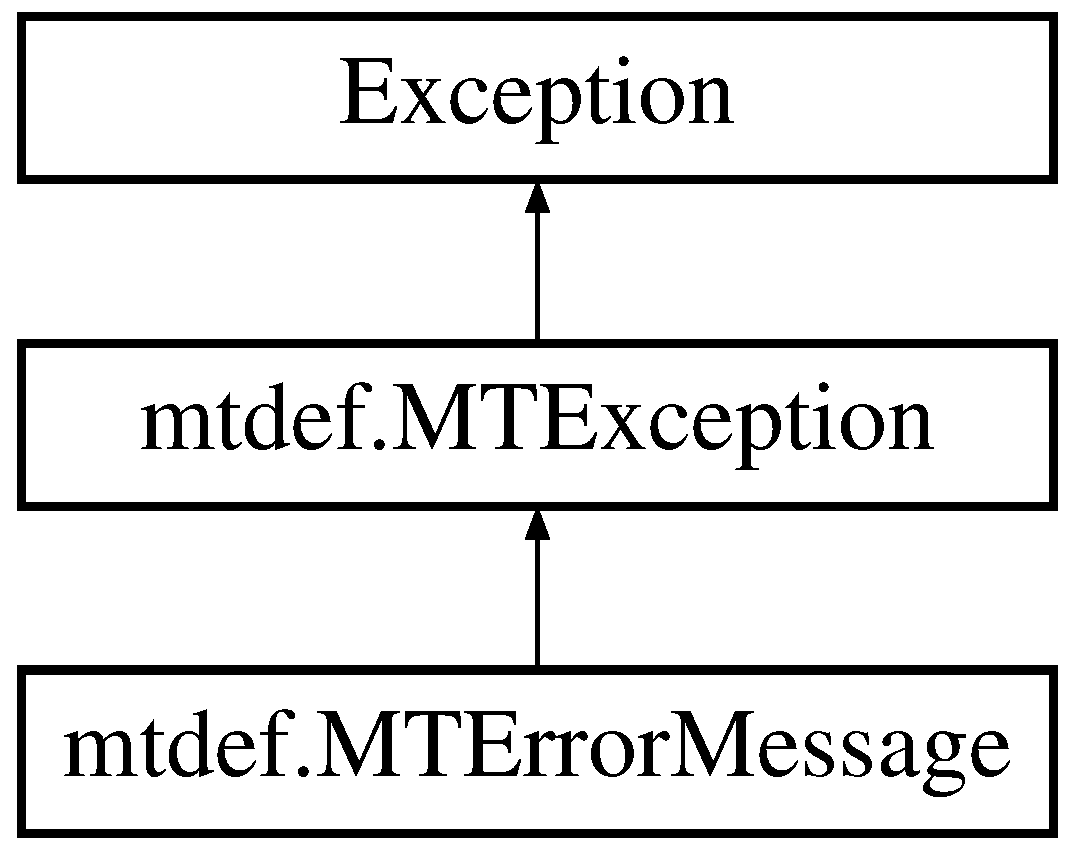
\includegraphics[height=3.000000cm]{classmtdef_1_1MTErrorMessage}
\end{center}
\end{figure}
\subsection*{Public Member Functions}
\begin{DoxyCompactItemize}
\item 
\mbox{\Hypertarget{classmtdef_1_1MTErrorMessage_ae64bba7a4863363c760725b93dc0ae80}\label{classmtdef_1_1MTErrorMessage_ae64bba7a4863363c760725b93dc0ae80}} 
def {\bfseries \+\_\+\+\_\+init\+\_\+\+\_\+} (self, code)
\item 
\mbox{\Hypertarget{classmtdef_1_1MTErrorMessage_a6b2ec6a3fc0618769ba588b72bbf2095}\label{classmtdef_1_1MTErrorMessage_a6b2ec6a3fc0618769ba588b72bbf2095}} 
def {\bfseries \+\_\+\+\_\+str\+\_\+\+\_\+} (self)
\end{DoxyCompactItemize}
\subsection*{Public Attributes}
\begin{DoxyCompactItemize}
\item 
\mbox{\Hypertarget{classmtdef_1_1MTErrorMessage_a09e96893fc730ac976b9ee2ac808b003}\label{classmtdef_1_1MTErrorMessage_a09e96893fc730ac976b9ee2ac808b003}} 
{\bfseries code}
\item 
\mbox{\Hypertarget{classmtdef_1_1MTErrorMessage_acd7e05bad351f6a79d3593d580790e2e}\label{classmtdef_1_1MTErrorMessage_acd7e05bad351f6a79d3593d580790e2e}} 
{\bfseries message}
\end{DoxyCompactItemize}
\subsection*{Static Public Attributes}
\begin{DoxyCompactItemize}
\item 
\mbox{\Hypertarget{classmtdef_1_1MTErrorMessage_a5bf79428ba751963956daa0258b277c4}\label{classmtdef_1_1MTErrorMessage_a5bf79428ba751963956daa0258b277c4}} 
dictionary {\bfseries Error\+Codes}
\end{DoxyCompactItemize}


The documentation for this class was generated from the following file\+:\begin{DoxyCompactItemize}
\item 
hardware\+\_\+layer/xsens\+\_\+driver/nodes/mtdef.\+py\end{DoxyCompactItemize}

\hypertarget{classmtdef_1_1MTException}{}\section{mtdef.\+M\+T\+Exception Class Reference}
\label{classmtdef_1_1MTException}\index{mtdef.\+M\+T\+Exception@{mtdef.\+M\+T\+Exception}}
Inheritance diagram for mtdef.\+M\+T\+Exception\+:\begin{figure}[H]
\begin{center}
\leavevmode
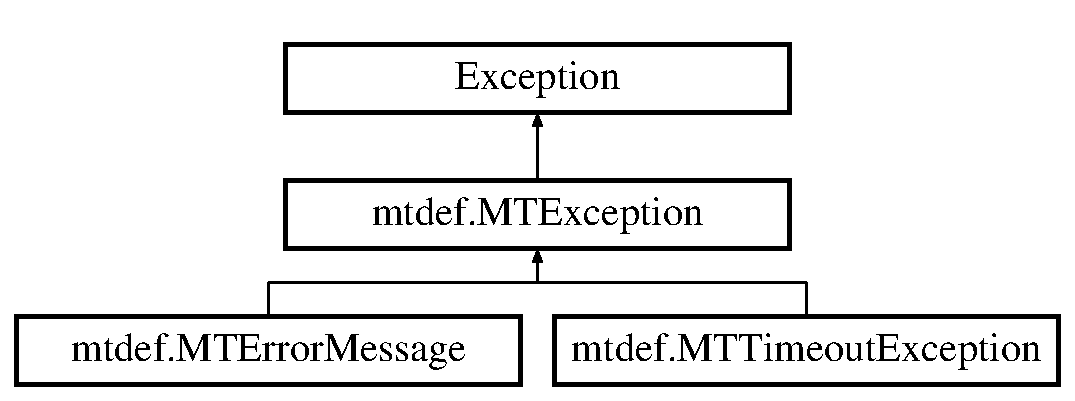
\includegraphics[height=3.000000cm]{classmtdef_1_1MTException}
\end{center}
\end{figure}
\subsection*{Public Member Functions}
\begin{DoxyCompactItemize}
\item 
\mbox{\Hypertarget{classmtdef_1_1MTException_aef2c8ab0a8238f7caee863fedbc6aa4a}\label{classmtdef_1_1MTException_aef2c8ab0a8238f7caee863fedbc6aa4a}} 
def {\bfseries \+\_\+\+\_\+init\+\_\+\+\_\+} (self, message)
\item 
\mbox{\Hypertarget{classmtdef_1_1MTException_ae945e5f5e231393ce05d1adc5d6cdd94}\label{classmtdef_1_1MTException_ae945e5f5e231393ce05d1adc5d6cdd94}} 
def {\bfseries \+\_\+\+\_\+str\+\_\+\+\_\+} (self)
\end{DoxyCompactItemize}
\subsection*{Public Attributes}
\begin{DoxyCompactItemize}
\item 
\mbox{\Hypertarget{classmtdef_1_1MTException_a5be6e05c2fd6b471ea167b25afad9f2d}\label{classmtdef_1_1MTException_a5be6e05c2fd6b471ea167b25afad9f2d}} 
{\bfseries message}
\end{DoxyCompactItemize}


The documentation for this class was generated from the following file\+:\begin{DoxyCompactItemize}
\item 
hardware\+\_\+layer/xsens\+\_\+driver/nodes/mtdef.\+py\end{DoxyCompactItemize}

\hypertarget{classmtdef_1_1MTTimeoutException}{}\doxysection{mtdef.\+M\+T\+Timeout\+Exception Class Reference}
\label{classmtdef_1_1MTTimeoutException}\index{mtdef.MTTimeoutException@{mtdef.MTTimeoutException}}
Inheritance diagram for mtdef.\+M\+T\+Timeout\+Exception\+:\begin{figure}[H]
\begin{center}
\leavevmode
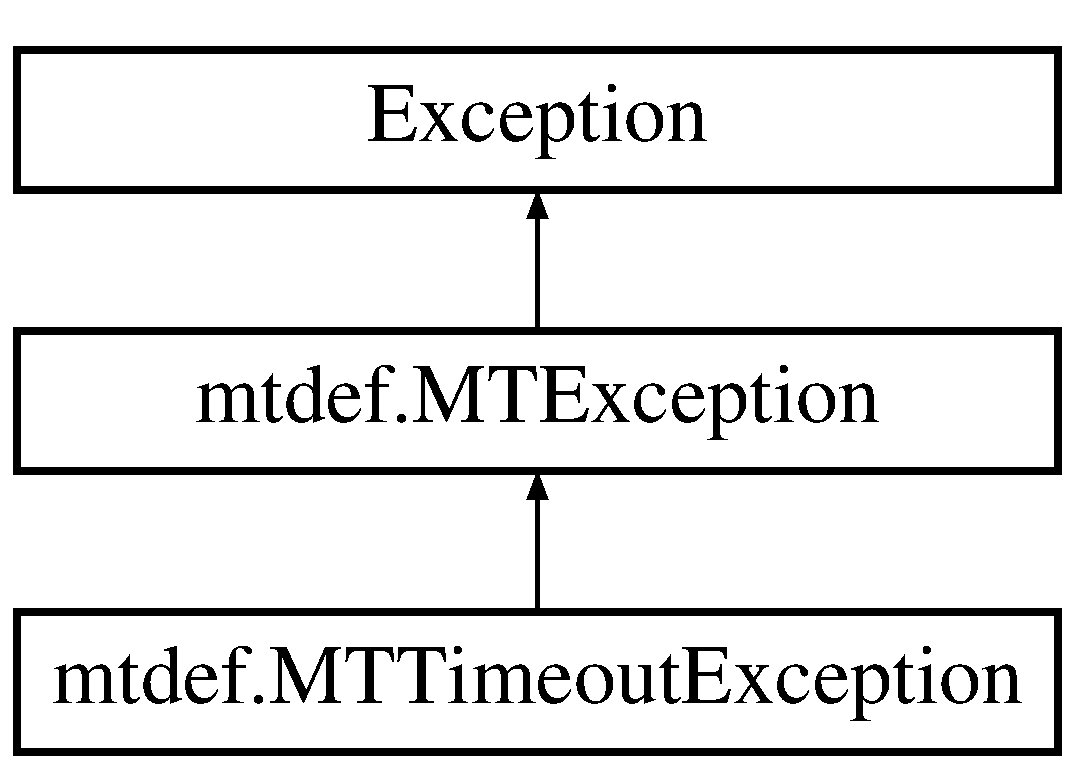
\includegraphics[height=3.000000cm]{classmtdef_1_1MTTimeoutException}
\end{center}
\end{figure}
\doxysubsection*{Public Member Functions}
\begin{DoxyCompactItemize}
\item 
\mbox{\Hypertarget{classmtdef_1_1MTTimeoutException_a229abababab998d9d19d36ee43dfc1c9}\label{classmtdef_1_1MTTimeoutException_a229abababab998d9d19d36ee43dfc1c9}} 
def {\bfseries \+\_\+\+\_\+init\+\_\+\+\_\+} (self, message)
\item 
\mbox{\Hypertarget{classmtdef_1_1MTTimeoutException_aed8d585a2f621e2b014daa2469f5ebbf}\label{classmtdef_1_1MTTimeoutException_aed8d585a2f621e2b014daa2469f5ebbf}} 
def {\bfseries \+\_\+\+\_\+str\+\_\+\+\_\+} (self)
\end{DoxyCompactItemize}
\doxysubsection*{Public Attributes}
\begin{DoxyCompactItemize}
\item 
\mbox{\Hypertarget{classmtdef_1_1MTTimeoutException_a6a33546be98bcca71867a978faa67e74}\label{classmtdef_1_1MTTimeoutException_a6a33546be98bcca71867a978faa67e74}} 
{\bfseries message}
\end{DoxyCompactItemize}


The documentation for this class was generated from the following file\+:\begin{DoxyCompactItemize}
\item 
hardware\+\_\+layer/xsens\+\_\+driver/nodes/mtdef.\+py\end{DoxyCompactItemize}

\hypertarget{classname}{}\doxysection{name Class Reference}
\label{classname}\index{name@{name}}


\doxysubsection{Detailed Description}
\mbox{]} \mbox{[}$<$header-\/name$>$\mbox{]} Ex-\/ /$\ast$! 

The documentation for this class was generated from the following file\+:\begin{DoxyCompactItemize}
\item 
coding\+\_\+docs/documentation.\+md\end{DoxyCompactItemize}

\hypertarget{classnavigation_1_1NavigationDevice}{}\section{navigation\+:\+:Navigation\+Device Class Reference}
\label{classnavigation_1_1NavigationDevice}\index{navigation\+::\+Navigation\+Device@{navigation\+::\+Navigation\+Device}}
Inheritance diagram for navigation\+:\+:Navigation\+Device\+:\begin{figure}[H]
\begin{center}
\leavevmode
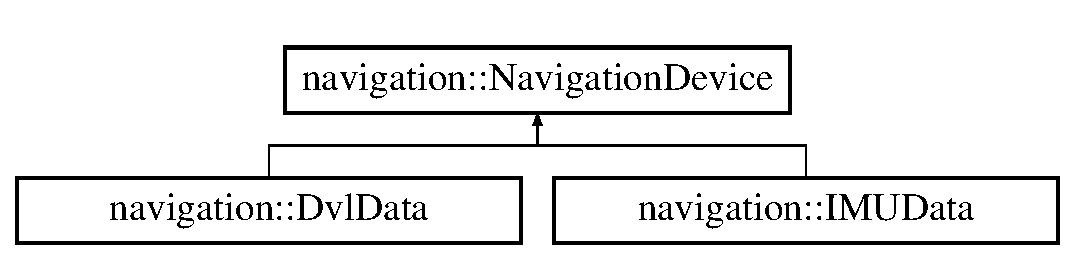
\includegraphics[height=2.000000cm]{classnavigation_1_1NavigationDevice}
\end{center}
\end{figure}
\subsection*{Public Member Functions}
\begin{DoxyCompactItemize}
\item 
\mbox{\Hypertarget{classnavigation_1_1NavigationDevice_ac4e032654f33b2a5dd3abd6294a0feb6}\label{classnavigation_1_1NavigationDevice_ac4e032654f33b2a5dd3abd6294a0feb6}} 
void {\bfseries Set\+New\+Data\+Ready} ()
\item 
\mbox{\Hypertarget{classnavigation_1_1NavigationDevice_a346b6be48e11c521c1f4b939ea86164b}\label{classnavigation_1_1NavigationDevice_a346b6be48e11c521c1f4b939ea86164b}} 
bool {\bfseries Is\+New\+Data\+Ready} ()
\item 
\mbox{\Hypertarget{classnavigation_1_1NavigationDevice_a8893fb5dce4975a994929fdb612acb7b}\label{classnavigation_1_1NavigationDevice_a8893fb5dce4975a994929fdb612acb7b}} 
void {\bfseries Set\+New\+Data\+Used} ()
\end{DoxyCompactItemize}


The documentation for this class was generated from the following file\+:\begin{DoxyCompactItemize}
\item 
navigation\+\_\+layer/odom\+\_\+dvl\+\_\+imu/include/navigation\+\_\+device.\+h\end{DoxyCompactItemize}

\hypertarget{classnavigation_1_1NavigationNode}{}\doxysection{navigation\+::Navigation\+Node Class Reference}
\label{classnavigation_1_1NavigationNode}\index{navigation::NavigationNode@{navigation::NavigationNode}}
\doxysubsection*{Public Member Functions}
\begin{DoxyCompactItemize}
\item 
\mbox{\Hypertarget{classnavigation_1_1NavigationNode_abccc1132cbda197d50c3e77318b54ef5}\label{classnavigation_1_1NavigationNode_abccc1132cbda197d50c3e77318b54ef5}} 
{\bfseries Navigation\+Node} (const ros\+::\+Node\+Handle\+Ptr \&nh)
\item 
\mbox{\Hypertarget{classnavigation_1_1NavigationNode_acfb226912b0b116ef2754286901f303e}\label{classnavigation_1_1NavigationNode_acfb226912b0b116ef2754286901f303e}} 
void {\bfseries Spin} ()
\item 
\mbox{\Hypertarget{classnavigation_1_1NavigationNode_af56f532c42808bca67db4fe71c7c7d2c}\label{classnavigation_1_1NavigationNode_af56f532c42808bca67db4fe71c7c7d2c}} 
void {\bfseries Process\+Cartesian\+Pose} ()
\item 
\mbox{\Hypertarget{classnavigation_1_1NavigationNode_a005d7dbd2eb1895f38992971a863edff}\label{classnavigation_1_1NavigationNode_a005d7dbd2eb1895f38992971a863edff}} 
void {\bfseries Publish\+Data} (ros\+::\+Time \&current\+\_\+time)
\item 
\mbox{\Hypertarget{classnavigation_1_1NavigationNode_ac52546f98124cdc13de5ab8930572e61}\label{classnavigation_1_1NavigationNode_ac52546f98124cdc13de5ab8930572e61}} 
void {\bfseries Broadcast\+Transform} (Eigen\+::\+Vector3d \&position, Eigen\+::\+Quaterniond \&quaternion, ros\+::\+Time \&current\+\_\+time)
\item 
\mbox{\Hypertarget{classnavigation_1_1NavigationNode_a1f8a76dd3fbda6df554b144515dd08cd}\label{classnavigation_1_1NavigationNode_a1f8a76dd3fbda6df554b144515dd08cd}} 
bool {\bfseries Set\+Depth\+Offset\+Callback} (odom\+\_\+dvl\+\_\+imu\+::\+Set\+Depth\+Offset\+::\+Request \&rqst, odom\+\_\+dvl\+\_\+imu\+::\+Set\+Depth\+Offset\+::\+Response \&response)
\item 
\mbox{\Hypertarget{classnavigation_1_1NavigationNode_aaefa2ce87f44e8b06462a8ebaae2bb25}\label{classnavigation_1_1NavigationNode_aaefa2ce87f44e8b06462a8ebaae2bb25}} 
bool {\bfseries Set\+World\+X\+Y\+Offset\+Callback} (odom\+\_\+dvl\+\_\+imu\+::\+Set\+World\+X\+Y\+Offset\+::\+Request \&rqst, odom\+\_\+dvl\+\_\+imu\+::\+Set\+World\+X\+Y\+Offset\+::\+Response \&response)
\item 
\mbox{\Hypertarget{classnavigation_1_1NavigationNode_a1b38cdb0bbb2e1661baea64022d8aeb9}\label{classnavigation_1_1NavigationNode_a1b38cdb0bbb2e1661baea64022d8aeb9}} 
void {\bfseries Fill\+Pose\+Msg} (Eigen\+::\+Vector3d \&position, Eigen\+::\+Quaterniond \&angle, nav\+\_\+msgs\+::\+Odometry \&msg)
\item 
\mbox{\Hypertarget{classnavigation_1_1NavigationNode_a42d3e7b88af64af00c794938c1f76439}\label{classnavigation_1_1NavigationNode_a42d3e7b88af64af00c794938c1f76439}} 
void {\bfseries Fill\+Twist\+Msg} (Eigen\+::\+Vector3d \&linear\+\_\+velocity, Eigen\+::\+Vector3d \&angular\+\_\+velocity, nav\+\_\+msgs\+::\+Odometry \&msg)
\end{DoxyCompactItemize}


The documentation for this class was generated from the following files\+:\begin{DoxyCompactItemize}
\item 
navigation\+\_\+layer/odom\+\_\+dvl\+\_\+imu/include/nav\+\_\+main.\+h\item 
navigation\+\_\+layer/odom\+\_\+dvl\+\_\+imu/src/nav\+\_\+main.\+cpp\end{DoxyCompactItemize}

\hypertarget{structObservation}{}\doxysection{Observation Struct Reference}
\label{structObservation}\index{Observation@{Observation}}
\doxysubsection*{Public Attributes}
\begin{DoxyCompactItemize}
\item 
\mbox{\Hypertarget{structObservation_a3fa8413ddbe7179997e74aab2a2f0af1}\label{structObservation_a3fa8413ddbe7179997e74aab2a2f0af1}} 
std\+::string {\bfseries id}
\item 
\mbox{\Hypertarget{structObservation_a12eaeea7a3843dcb54da2bb94dec6f0d}\label{structObservation_a12eaeea7a3843dcb54da2bb94dec6f0d}} 
int {\bfseries m\+\_\+x}
\item 
\mbox{\Hypertarget{structObservation_a8e44bae27bba19c334bedd16a76080cb}\label{structObservation_a8e44bae27bba19c334bedd16a76080cb}} 
int {\bfseries m\+\_\+y}
\item 
\mbox{\Hypertarget{structObservation_a8ed13bbc80cae27bb62182b96dd9c123}\label{structObservation_a8ed13bbc80cae27bb62182b96dd9c123}} 
int {\bfseries m\+\_\+z}
\item 
\mbox{\Hypertarget{structObservation_ac814a20a30fc3434bced8543493770d1}\label{structObservation_ac814a20a30fc3434bced8543493770d1}} 
int {\bfseries u\+\_\+x}
\item 
\mbox{\Hypertarget{structObservation_a5ef35caea2cff7d0eacb989659919cbb}\label{structObservation_a5ef35caea2cff7d0eacb989659919cbb}} 
int {\bfseries u\+\_\+y}
\item 
\mbox{\Hypertarget{structObservation_a10c8f97f0fc5b5ebb9ee13d2f8b389a4}\label{structObservation_a10c8f97f0fc5b5ebb9ee13d2f8b389a4}} 
int {\bfseries u\+\_\+z}
\end{DoxyCompactItemize}


The documentation for this struct was generated from the following file\+:\begin{DoxyCompactItemize}
\item 
navigation\+\_\+layer/mapping/include/util.\+h\end{DoxyCompactItemize}

\hypertarget{classOctagon}{}\doxysection{Octagon Class Reference}
\label{classOctagon}\index{Octagon@{Octagon}}
Inheritance diagram for Octagon\+:\begin{figure}[H]
\begin{center}
\leavevmode
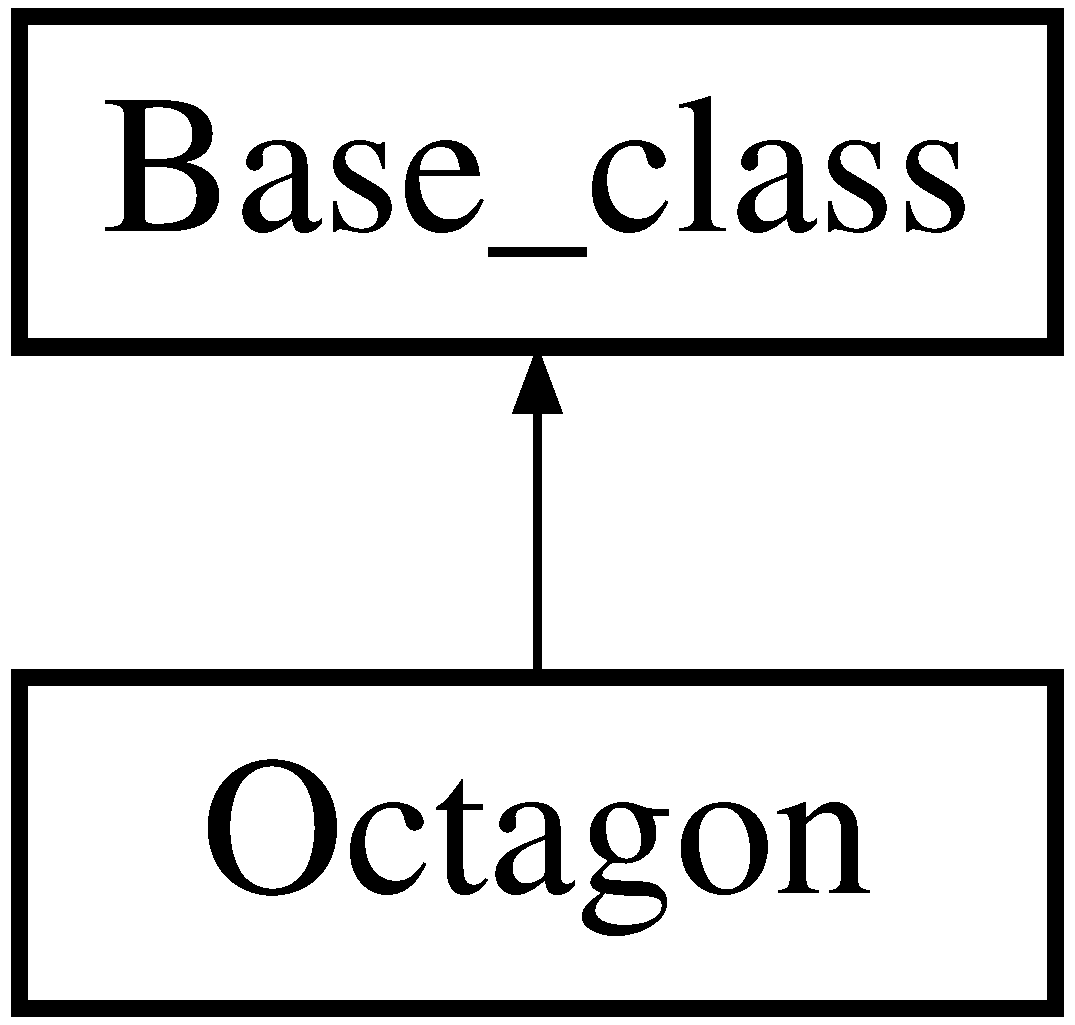
\includegraphics[height=2.000000cm]{classOctagon}
\end{center}
\end{figure}
\doxysubsection*{Public Member Functions}
\begin{DoxyCompactItemize}
\item 
\mbox{\Hypertarget{classOctagon_ae6a83e650bae938f9ab63abcfd58a398}\label{classOctagon_ae6a83e650bae938f9ab63abcfd58a398}} 
void {\bfseries spin\+Thread\+Bottom} ()
\item 
\mbox{\Hypertarget{classOctagon_a4a7d77e22163d6ee6c1f11210ed2a61d}\label{classOctagon_a4a7d77e22163d6ee6c1f11210ed2a61d}} 
void {\bfseries spin\+Thread\+Front} ()
\end{DoxyCompactItemize}
\doxysubsection*{Protected Member Functions}
\begin{DoxyCompactItemize}
\item 
\mbox{\Hypertarget{classOctagon_a7a1450a53ab430cbdf013159e837c848}\label{classOctagon_a7a1450a53ab430cbdf013159e837c848}} 
void {\bfseries front\+Callback} (vision\+\_\+tasks\+::octagon\+Front\+Range\+Config \&config, double level)
\item 
\mbox{\Hypertarget{classOctagon_ad953bf1ace4c8a2d09f364a096030df4}\label{classOctagon_ad953bf1ace4c8a2d09f364a096030df4}} 
void {\bfseries bottom\+Callback} (vision\+\_\+tasks\+::octagon\+Bottom\+Range\+Config \&config, double level)
\item 
\mbox{\Hypertarget{classOctagon_a3840f97fdb1c59d6a9015e7502a94a4d}\label{classOctagon_a3840f97fdb1c59d6a9015e7502a94a4d}} 
void {\bfseries image\+Front\+Callback} (const sensor\+\_\+msgs\+::\+Image\+::\+Const\+Ptr \&msg)
\item 
\mbox{\Hypertarget{classOctagon_a4c98afeabdf2d48a7a794cf58dba3e93}\label{classOctagon_a4c98afeabdf2d48a7a794cf58dba3e93}} 
void {\bfseries image\+Bottom\+Callback} (const sensor\+\_\+msgs\+::\+Image\+::\+Const\+Ptr \&msg)
\end{DoxyCompactItemize}
\doxysubsection*{Protected Attributes}
\begin{DoxyCompactItemize}
\item 
\mbox{\Hypertarget{classOctagon_ad81ad65b8cfd994d4c8e9ff920cbbc72}\label{classOctagon_ad81ad65b8cfd994d4c8e9ff920cbbc72}} 
image\+\_\+transport\+::\+Publisher {\bfseries blue\+\_\+filtered\+\_\+pub}
\item 
\mbox{\Hypertarget{classOctagon_ac730f845f82658b1cad679699d492878}\label{classOctagon_ac730f845f82658b1cad679699d492878}} 
image\+\_\+transport\+::\+Subscriber {\bfseries image\+\_\+raw\+\_\+sub}
\item 
\mbox{\Hypertarget{classOctagon_a134b4a5d27fa1f771c928a2cf2441eac}\label{classOctagon_a134b4a5d27fa1f771c928a2cf2441eac}} 
std\+::string {\bfseries camera\+\_\+frame\+\_\+}
\item 
\mbox{\Hypertarget{classOctagon_a18101d0809a701a880a71da13a867c32}\label{classOctagon_a18101d0809a701a880a71da13a867c32}} 
double {\bfseries front\+\_\+clahe\+\_\+clip\+\_\+} = 4.\+0
\item 
\mbox{\Hypertarget{classOctagon_a7ac3f3216b3b65a631e2966d9fe947d6}\label{classOctagon_a7ac3f3216b3b65a631e2966d9fe947d6}} 
int {\bfseries front\+\_\+clahe\+\_\+grid\+\_\+size\+\_\+} = 8
\item 
\mbox{\Hypertarget{classOctagon_a37e874f2b6b0defbadf34637e655d462}\label{classOctagon_a37e874f2b6b0defbadf34637e655d462}} 
int {\bfseries front\+\_\+clahe\+\_\+bilateral\+\_\+iter\+\_\+} = 8
\item 
\mbox{\Hypertarget{classOctagon_a6526833743c9afd65cbed7e5b2f54168}\label{classOctagon_a6526833743c9afd65cbed7e5b2f54168}} 
int {\bfseries front\+\_\+balanced\+\_\+bilateral\+\_\+iter\+\_\+} = 4
\item 
\mbox{\Hypertarget{classOctagon_a71822dfc8d160896ff4193935ec78a0e}\label{classOctagon_a71822dfc8d160896ff4193935ec78a0e}} 
double {\bfseries front\+\_\+denoise\+\_\+h\+\_\+} = 10.\+0
\item 
\mbox{\Hypertarget{classOctagon_a65a3ea1eb703a5c45abcac586e190bbc}\label{classOctagon_a65a3ea1eb703a5c45abcac586e190bbc}} 
int {\bfseries front\+\_\+canny\+\_\+threshold\+\_\+low\+\_\+} = 0
\item 
\mbox{\Hypertarget{classOctagon_a588fd8490c6e59ba0c59b8c0c0def6dc}\label{classOctagon_a588fd8490c6e59ba0c59b8c0c0def6dc}} 
int {\bfseries front\+\_\+canny\+\_\+threshold\+\_\+high\+\_\+} = 1000
\item 
\mbox{\Hypertarget{classOctagon_ae20ae84d732e1d108b9f9ebef17a15e0}\label{classOctagon_ae20ae84d732e1d108b9f9ebef17a15e0}} 
int {\bfseries front\+\_\+canny\+\_\+kernel\+\_\+size\+\_\+} = 3
\item 
\mbox{\Hypertarget{classOctagon_a38dc6d16117d852010885329488f2c22}\label{classOctagon_a38dc6d16117d852010885329488f2c22}} 
int {\bfseries front\+\_\+hough\+\_\+threshold\+\_\+} = 0
\item 
\mbox{\Hypertarget{classOctagon_afd0747af826ceb68845a97e5845c6474}\label{classOctagon_afd0747af826ceb68845a97e5845c6474}} 
int {\bfseries front\+\_\+hough\+\_\+minline\+\_\+} = 0
\item 
\mbox{\Hypertarget{classOctagon_a5784640d78bd54b9d3f804e6971485bb}\label{classOctagon_a5784640d78bd54b9d3f804e6971485bb}} 
int {\bfseries front\+\_\+hough\+\_\+maxgap\+\_\+} = 0
\item 
\mbox{\Hypertarget{classOctagon_af676c0a43e9a80e80e6594afbefca004}\label{classOctagon_af676c0a43e9a80e80e6594afbefca004}} 
double {\bfseries front\+\_\+hough\+\_\+angle\+\_\+tolerance\+\_\+} = 0.\+0
\item 
\mbox{\Hypertarget{classOctagon_a06d4848d0fa2f540bcebb40af1d96dda}\label{classOctagon_a06d4848d0fa2f540bcebb40af1d96dda}} 
double {\bfseries front\+\_\+gate\+\_\+distance\+\_\+tolerance\+\_\+} = 50.\+0
\item 
\mbox{\Hypertarget{classOctagon_a8603b04b031ae06fb38e51306a05e8ba}\label{classOctagon_a8603b04b031ae06fb38e51306a05e8ba}} 
double {\bfseries front\+\_\+gate\+\_\+angle\+\_\+tolerance\+\_\+} = 0.\+0
\item 
\mbox{\Hypertarget{classOctagon_a7bfa15dbbdf5f98fecc84d32ea88ab6c}\label{classOctagon_a7bfa15dbbdf5f98fecc84d32ea88ab6c}} 
double {\bfseries bottom\+\_\+clahe\+\_\+clip\+\_\+} = 4.\+0
\item 
\mbox{\Hypertarget{classOctagon_a8a4311d54b59371229c84ce0b30fb9eb}\label{classOctagon_a8a4311d54b59371229c84ce0b30fb9eb}} 
int {\bfseries bottom\+\_\+clahe\+\_\+grid\+\_\+size\+\_\+} = 8
\item 
\mbox{\Hypertarget{classOctagon_aa393f9dec40f6f21d4a49db75d0d30aa}\label{classOctagon_aa393f9dec40f6f21d4a49db75d0d30aa}} 
int {\bfseries bottom\+\_\+clahe\+\_\+bilateral\+\_\+iter\+\_\+} = 8
\item 
\mbox{\Hypertarget{classOctagon_ae61cbe0134eed2dac3ef1ac66ebb919b}\label{classOctagon_ae61cbe0134eed2dac3ef1ac66ebb919b}} 
int {\bfseries bottom\+\_\+balanced\+\_\+bilateral\+\_\+iter\+\_\+} = 4
\item 
\mbox{\Hypertarget{classOctagon_a359e6996f9cf84c6938d36f96fa12ded}\label{classOctagon_a359e6996f9cf84c6938d36f96fa12ded}} 
double {\bfseries bottom\+\_\+denoise\+\_\+h\+\_\+} = 10.\+0
\item 
\mbox{\Hypertarget{classOctagon_ad9021e5849858697ae198c657ea268ae}\label{classOctagon_ad9021e5849858697ae198c657ea268ae}} 
bool {\bfseries task\+\_\+done} = false
\end{DoxyCompactItemize}
\doxysubsection*{Additional Inherited Members}


The documentation for this class was generated from the following files\+:\begin{DoxyCompactItemize}
\item 
vision\+\_\+layer/vision\+\_\+tasks/include/octagon.\+h\item 
vision\+\_\+layer/vision\+\_\+tasks/src/octagon.\+cpp\end{DoxyCompactItemize}

\hypertarget{classmaster__layer_1_1state__mach__gate__torpedo_1_1OctagonTask}{}\section{master\+\_\+layer.\+state\+\_\+mach\+\_\+gate\+\_\+torpedo.\+Octagon\+Task Class Reference}
\label{classmaster__layer_1_1state__mach__gate__torpedo_1_1OctagonTask}\index{master\+\_\+layer.\+state\+\_\+mach\+\_\+gate\+\_\+torpedo.\+Octagon\+Task@{master\+\_\+layer.\+state\+\_\+mach\+\_\+gate\+\_\+torpedo.\+Octagon\+Task}}
Inheritance diagram for master\+\_\+layer.\+state\+\_\+mach\+\_\+gate\+\_\+torpedo.\+Octagon\+Task\+:\begin{figure}[H]
\begin{center}
\leavevmode
\includegraphics[height=3.000000cm]{classmaster__layer_1_1state__mach__gate__torpedo_1_1OctagonTask}
\end{center}
\end{figure}
\subsection*{Public Member Functions}
\begin{DoxyCompactItemize}
\item 
\mbox{\Hypertarget{classmaster__layer_1_1state__mach__gate__torpedo_1_1OctagonTask_a7285cf08473e623a36d1ecf143bf236b}\label{classmaster__layer_1_1state__mach__gate__torpedo_1_1OctagonTask_a7285cf08473e623a36d1ecf143bf236b}} 
def {\bfseries \+\_\+\+\_\+init\+\_\+\+\_\+} (self)
\item 
\mbox{\Hypertarget{classmaster__layer_1_1state__mach__gate__torpedo_1_1OctagonTask_a690860c6b63feeffc2daaa1b8cb24c53}\label{classmaster__layer_1_1state__mach__gate__torpedo_1_1OctagonTask_a690860c6b63feeffc2daaa1b8cb24c53}} 
def {\bfseries localise} (self)
\item 
\mbox{\Hypertarget{classmaster__layer_1_1state__mach__gate__torpedo_1_1OctagonTask_a4d5108b47fdc3fb8e529c8ed8d123fd7}\label{classmaster__layer_1_1state__mach__gate__torpedo_1_1OctagonTask_a4d5108b47fdc3fb8e529c8ed8d123fd7}} 
def {\bfseries execute} (self)
\end{DoxyCompactItemize}


The documentation for this class was generated from the following file\+:\begin{DoxyCompactItemize}
\item 
master\+\_\+layer/src/master\+\_\+layer/state\+\_\+mach\+\_\+gate\+\_\+torpedo.\+py\end{DoxyCompactItemize}

\hypertarget{classmaster__layer_1_1state__mach_1_1OctagonTask}{}\doxysection{master\+\_\+layer.\+state\+\_\+mach.\+Octagon\+Task Class Reference}
\label{classmaster__layer_1_1state__mach_1_1OctagonTask}\index{master\_layer.state\_mach.OctagonTask@{master\_layer.state\_mach.OctagonTask}}
Inheritance diagram for master\+\_\+layer.\+state\+\_\+mach.\+Octagon\+Task\+:\begin{figure}[H]
\begin{center}
\leavevmode
\includegraphics[height=3.000000cm]{classmaster__layer_1_1state__mach_1_1OctagonTask}
\end{center}
\end{figure}
\doxysubsection*{Public Member Functions}
\begin{DoxyCompactItemize}
\item 
\mbox{\Hypertarget{classmaster__layer_1_1state__mach_1_1OctagonTask_aab8fd91555f8d6962c7cf2199132c8f8}\label{classmaster__layer_1_1state__mach_1_1OctagonTask_aab8fd91555f8d6962c7cf2199132c8f8}} 
def {\bfseries \+\_\+\+\_\+init\+\_\+\+\_\+} (self)
\item 
\mbox{\Hypertarget{classmaster__layer_1_1state__mach_1_1OctagonTask_ae291b244ebd1e04d10b3e56a05728a53}\label{classmaster__layer_1_1state__mach_1_1OctagonTask_ae291b244ebd1e04d10b3e56a05728a53}} 
def {\bfseries localise} (self)
\item 
\mbox{\Hypertarget{classmaster__layer_1_1state__mach_1_1OctagonTask_a7171d42a13de1ae33c8855b84ac5379d}\label{classmaster__layer_1_1state__mach_1_1OctagonTask_a7171d42a13de1ae33c8855b84ac5379d}} 
def {\bfseries execute} (self)
\end{DoxyCompactItemize}


The documentation for this class was generated from the following file\+:\begin{DoxyCompactItemize}
\item 
master\+\_\+layer/src/master\+\_\+layer/state\+\_\+mach.\+py\end{DoxyCompactItemize}

\hypertarget{classimage__undistort_1_1OutputCameraParameters}{}\doxysection{image\+\_\+undistort\+::Output\+Camera\+Parameters Class Reference}
\label{classimage__undistort_1_1OutputCameraParameters}\index{image\_undistort::OutputCameraParameters@{image\_undistort::OutputCameraParameters}}
Inheritance diagram for image\+\_\+undistort\+::Output\+Camera\+Parameters\+:\begin{figure}[H]
\begin{center}
\leavevmode
\includegraphics[height=2.000000cm]{classimage__undistort_1_1OutputCameraParameters}
\end{center}
\end{figure}
\doxysubsection*{Public Member Functions}
\begin{DoxyCompactItemize}
\item 
\mbox{\Hypertarget{classimage__undistort_1_1OutputCameraParameters_a88a33425ade97a10aabdae322da2b72b}\label{classimage__undistort_1_1OutputCameraParameters_a88a33425ade97a10aabdae322da2b72b}} 
{\bfseries Base\+Camera\+Parameters} (const ros\+::\+Node\+Handle \&nh, const std\+::string \&camera\+\_\+namespace, const bool invert\+\_\+T)
\item 
\mbox{\Hypertarget{classimage__undistort_1_1OutputCameraParameters_a542e183ba91d54f0ec7f7e5aef5b41c4}\label{classimage__undistort_1_1OutputCameraParameters_a542e183ba91d54f0ec7f7e5aef5b41c4}} 
{\bfseries Base\+Camera\+Parameters} (const sensor\+\_\+msgs\+::\+Camera\+Info \&camera\+\_\+info)
\item 
\mbox{\Hypertarget{classimage__undistort_1_1OutputCameraParameters_a1da0c8f547d638bd1ca788210fd60618}\label{classimage__undistort_1_1OutputCameraParameters_a1da0c8f547d638bd1ca788210fd60618}} 
{\bfseries Base\+Camera\+Parameters} (const cv\+::\+Size \&resolution\+\_\+in, const Eigen\+::\+Matrix$<$ double, 4, 4 $>$ \&T\+\_\+in, const Eigen\+::\+Matrix$<$ double, 3, 3 $>$ \&K\+\_\+in)
\end{DoxyCompactItemize}


The documentation for this class was generated from the following file\+:\begin{DoxyCompactItemize}
\item 
vision\+\_\+layer/image\+\_\+undistort/include/image\+\_\+undistort/camera\+\_\+parameters.\+h\end{DoxyCompactItemize}

\hypertarget{classmtdef_1_1OutputMode}{}\section{mtdef.\+Output\+Mode Class Reference}
\label{classmtdef_1_1OutputMode}\index{mtdef.\+Output\+Mode@{mtdef.\+Output\+Mode}}
\subsection*{Static Public Attributes}
\begin{DoxyCompactItemize}
\item 
\mbox{\Hypertarget{classmtdef_1_1OutputMode_ac5c68dcf874d1e2982a8296727639e54}\label{classmtdef_1_1OutputMode_ac5c68dcf874d1e2982a8296727639e54}} 
int {\bfseries Temp} = 0x0001
\item 
\mbox{\Hypertarget{classmtdef_1_1OutputMode_a6f5d09a03cade7d3a04d07cb487520e3}\label{classmtdef_1_1OutputMode_a6f5d09a03cade7d3a04d07cb487520e3}} 
int {\bfseries Calib} = 0x0002
\item 
\mbox{\Hypertarget{classmtdef_1_1OutputMode_a031a1c61927f3039f6d9271fae79be36}\label{classmtdef_1_1OutputMode_a031a1c61927f3039f6d9271fae79be36}} 
int {\bfseries Orient} = 0x0004
\item 
\mbox{\Hypertarget{classmtdef_1_1OutputMode_a9e5152e494ecf666df741c9999cbc777}\label{classmtdef_1_1OutputMode_a9e5152e494ecf666df741c9999cbc777}} 
int {\bfseries Auxiliary} = 0x0008
\item 
\mbox{\Hypertarget{classmtdef_1_1OutputMode_acaf9bc94db44bd7286444d26c77f2d58}\label{classmtdef_1_1OutputMode_acaf9bc94db44bd7286444d26c77f2d58}} 
int {\bfseries Position} = 0x0010
\item 
\mbox{\Hypertarget{classmtdef_1_1OutputMode_afd059ee03dd482940f9fdcd40247aef4}\label{classmtdef_1_1OutputMode_afd059ee03dd482940f9fdcd40247aef4}} 
int {\bfseries Velocity} = 0x0020
\item 
\mbox{\Hypertarget{classmtdef_1_1OutputMode_a2008da9ce384717cd66f084d25779160}\label{classmtdef_1_1OutputMode_a2008da9ce384717cd66f084d25779160}} 
int {\bfseries Status} = 0x0800
\item 
\mbox{\Hypertarget{classmtdef_1_1OutputMode_a71c49d935984f8be8cfebbf2ed577cf0}\label{classmtdef_1_1OutputMode_a71c49d935984f8be8cfebbf2ed577cf0}} 
int {\bfseries R\+A\+W\+G\+PS} = 0x1000
\item 
\mbox{\Hypertarget{classmtdef_1_1OutputMode_afcadd4cfb477338178688ab2d8ed7062}\label{classmtdef_1_1OutputMode_afcadd4cfb477338178688ab2d8ed7062}} 
int {\bfseries R\+AW} = 0x4000
\end{DoxyCompactItemize}


\subsection{Detailed Description}
\begin{DoxyVerb}Values for the output mode.\end{DoxyVerb}
 

The documentation for this class was generated from the following file\+:\begin{DoxyCompactItemize}
\item 
hardware\+\_\+layer/xsens\+\_\+driver/nodes/mtdef.\+py\end{DoxyCompactItemize}

\hypertarget{classmtdef_1_1OutputSettings}{}\section{mtdef.\+Output\+Settings Class Reference}
\label{classmtdef_1_1OutputSettings}\index{mtdef.\+Output\+Settings@{mtdef.\+Output\+Settings}}
\subsection*{Static Public Attributes}
\begin{DoxyCompactItemize}
\item 
\mbox{\Hypertarget{classmtdef_1_1OutputSettings_a21f6a1e444c2314ff883095fe41e248a}\label{classmtdef_1_1OutputSettings_a21f6a1e444c2314ff883095fe41e248a}} 
int {\bfseries Timestamp\+\_\+\+None} = 0x00000000
\item 
\mbox{\Hypertarget{classmtdef_1_1OutputSettings_aa7e0d190ce08cac459f4042cc7638546}\label{classmtdef_1_1OutputSettings_aa7e0d190ce08cac459f4042cc7638546}} 
int {\bfseries Timestamp\+\_\+\+Sample\+Cnt} = 0x00000001
\item 
\mbox{\Hypertarget{classmtdef_1_1OutputSettings_a45702b3c952f82ee815f80d4ddf67acd}\label{classmtdef_1_1OutputSettings_a45702b3c952f82ee815f80d4ddf67acd}} 
int {\bfseries Timestamp\+\_\+\+U\+T\+C\+Time} = 0x00000002
\item 
\mbox{\Hypertarget{classmtdef_1_1OutputSettings_ae7c4548b20142c4fc887572f61516c01}\label{classmtdef_1_1OutputSettings_ae7c4548b20142c4fc887572f61516c01}} 
int {\bfseries Orient\+Mode\+\_\+\+Quaternion} = 0x00000000
\item 
\mbox{\Hypertarget{classmtdef_1_1OutputSettings_ac88d29ef6f18690b6837490d0ea31437}\label{classmtdef_1_1OutputSettings_ac88d29ef6f18690b6837490d0ea31437}} 
int {\bfseries Orient\+Mode\+\_\+\+Euler} = 0x00000004
\item 
\mbox{\Hypertarget{classmtdef_1_1OutputSettings_a0e7cdac578699e9bc8fad8a34a0904aa}\label{classmtdef_1_1OutputSettings_a0e7cdac578699e9bc8fad8a34a0904aa}} 
int {\bfseries Orient\+Mode\+\_\+\+Matrix} = 0x00000008
\item 
\mbox{\Hypertarget{classmtdef_1_1OutputSettings_a617223f5f925678751276e19bf1d4e7a}\label{classmtdef_1_1OutputSettings_a617223f5f925678751276e19bf1d4e7a}} 
int {\bfseries Calib\+Mode\+\_\+\+Acc\+Gyr\+Mag} = 0x00000000
\item 
\mbox{\Hypertarget{classmtdef_1_1OutputSettings_a2cc8f0cde270b93e5edcb0014f8c8ff4}\label{classmtdef_1_1OutputSettings_a2cc8f0cde270b93e5edcb0014f8c8ff4}} 
int {\bfseries Calib\+Mode\+\_\+\+Gyr\+Mag} = 0x00000010
\item 
\mbox{\Hypertarget{classmtdef_1_1OutputSettings_ab380665552dcd523ab3fac5ccdc97a46}\label{classmtdef_1_1OutputSettings_ab380665552dcd523ab3fac5ccdc97a46}} 
int {\bfseries Calib\+Mode\+\_\+\+Acc\+Mag} = 0x00000020
\item 
\mbox{\Hypertarget{classmtdef_1_1OutputSettings_a059e574b52794edab0de678d5d4de371}\label{classmtdef_1_1OutputSettings_a059e574b52794edab0de678d5d4de371}} 
int {\bfseries Calib\+Mode\+\_\+\+Mag} = 0x00000030
\item 
\mbox{\Hypertarget{classmtdef_1_1OutputSettings_a3e8a8b3d4f3920f029cb283c04d3ac03}\label{classmtdef_1_1OutputSettings_a3e8a8b3d4f3920f029cb283c04d3ac03}} 
int {\bfseries Calib\+Mode\+\_\+\+Acc\+Gyr} = 0x00000040
\item 
\mbox{\Hypertarget{classmtdef_1_1OutputSettings_a6719a0b0acf6295ffcf1c6f6ffc25a50}\label{classmtdef_1_1OutputSettings_a6719a0b0acf6295ffcf1c6f6ffc25a50}} 
int {\bfseries Calib\+Mode\+\_\+\+Gyr} = 0x00000050
\item 
\mbox{\Hypertarget{classmtdef_1_1OutputSettings_acf70ec170717970c35a02419060b5934}\label{classmtdef_1_1OutputSettings_acf70ec170717970c35a02419060b5934}} 
int {\bfseries Calib\+Mode\+\_\+\+Acc} = 0x00000060
\item 
\mbox{\Hypertarget{classmtdef_1_1OutputSettings_abca3164def620098dd83148e0ddd3e35}\label{classmtdef_1_1OutputSettings_abca3164def620098dd83148e0ddd3e35}} 
int {\bfseries Calib\+Mode\+\_\+\+Mask} = 0x00000070
\item 
\mbox{\Hypertarget{classmtdef_1_1OutputSettings_a75fed1781a0cfc09ea19d27573496e21}\label{classmtdef_1_1OutputSettings_a75fed1781a0cfc09ea19d27573496e21}} 
int {\bfseries Data\+Format\+\_\+\+Float} = 0x00000000
\item 
\mbox{\Hypertarget{classmtdef_1_1OutputSettings_add84144c4d3bb546c5ff77622ac2436b}\label{classmtdef_1_1OutputSettings_add84144c4d3bb546c5ff77622ac2436b}} 
int {\bfseries Data\+Format\+\_\+12\+\_\+20} = 0x00000100
\item 
\mbox{\Hypertarget{classmtdef_1_1OutputSettings_ab2ed6d90b58a1d46c30190e0e70857bf}\label{classmtdef_1_1OutputSettings_ab2ed6d90b58a1d46c30190e0e70857bf}} 
int {\bfseries Data\+Format\+\_\+16\+\_\+32} = 0x00000200
\item 
\mbox{\Hypertarget{classmtdef_1_1OutputSettings_ad93964f9527bf4e1c40cda7e544c16a4}\label{classmtdef_1_1OutputSettings_ad93964f9527bf4e1c40cda7e544c16a4}} 
int {\bfseries Data\+Format\+\_\+\+Double} = 0x00000300
\item 
\mbox{\Hypertarget{classmtdef_1_1OutputSettings_ac56523c098fe50984c5f140843eb1e91}\label{classmtdef_1_1OutputSettings_ac56523c098fe50984c5f140843eb1e91}} 
int {\bfseries Auxiliary\+Mode\+\_\+\+No\+A\+I\+N1} = 0x00000400
\item 
\mbox{\Hypertarget{classmtdef_1_1OutputSettings_a9b5d05844eb4be1d2cf172085df00acf}\label{classmtdef_1_1OutputSettings_a9b5d05844eb4be1d2cf172085df00acf}} 
int {\bfseries Auxiliary\+Mode\+\_\+\+No\+A\+I\+N2} = 0x00000800
\item 
\mbox{\Hypertarget{classmtdef_1_1OutputSettings_ab62dd60f5832688443a2e45b4cb2d0fc}\label{classmtdef_1_1OutputSettings_ab62dd60f5832688443a2e45b4cb2d0fc}} 
int {\bfseries Position\+Mode\+\_\+\+L\+L\+A\+\_\+\+W\+G\+S84} = 0x00000000
\item 
\mbox{\Hypertarget{classmtdef_1_1OutputSettings_a59cb8d9ae30e9a5706ecf85e3bd8fc82}\label{classmtdef_1_1OutputSettings_a59cb8d9ae30e9a5706ecf85e3bd8fc82}} 
int {\bfseries Velocity\+Mode\+\_\+\+M\+S\+\_\+\+X\+YZ} = 0x00000000
\item 
\mbox{\Hypertarget{classmtdef_1_1OutputSettings_a7fe2d76eb7a97487ef2a9aa47c82ec1c}\label{classmtdef_1_1OutputSettings_a7fe2d76eb7a97487ef2a9aa47c82ec1c}} 
int {\bfseries Coordinates\+\_\+\+N\+ED} = 0x80000000
\end{DoxyCompactItemize}


\subsection{Detailed Description}
\begin{DoxyVerb}Values for the output settings.\end{DoxyVerb}
 

The documentation for this class was generated from the following file\+:\begin{DoxyCompactItemize}
\item 
hardware\+\_\+layer/xsens\+\_\+driver/nodes/mtdef.\+py\end{DoxyCompactItemize}

\hypertarget{classuuv__trajectory__generator_1_1path__generator_1_1path__generator_1_1PathGenerator}{}\section{uuv\+\_\+trajectory\+\_\+generator.\+path\+\_\+generator.\+path\+\_\+generator.\+Path\+Generator Class Reference}
\label{classuuv__trajectory__generator_1_1path__generator_1_1path__generator_1_1PathGenerator}\index{uuv\+\_\+trajectory\+\_\+generator.\+path\+\_\+generator.\+path\+\_\+generator.\+Path\+Generator@{uuv\+\_\+trajectory\+\_\+generator.\+path\+\_\+generator.\+path\+\_\+generator.\+Path\+Generator}}
Inheritance diagram for uuv\+\_\+trajectory\+\_\+generator.\+path\+\_\+generator.\+path\+\_\+generator.\+Path\+Generator\+:\begin{figure}[H]
\begin{center}
\leavevmode
\includegraphics[height=0.887949cm]{classuuv__trajectory__generator_1_1path__generator_1_1path__generator_1_1PathGenerator}
\end{center}
\end{figure}
\subsection*{Public Member Functions}
\begin{DoxyCompactItemize}
\item 
\mbox{\Hypertarget{classuuv__trajectory__generator_1_1path__generator_1_1path__generator_1_1PathGenerator_ae256fd2600082519cf221ac47e843177}\label{classuuv__trajectory__generator_1_1path__generator_1_1path__generator_1_1PathGenerator_ae256fd2600082519cf221ac47e843177}} 
def {\bfseries \+\_\+\+\_\+init\+\_\+\+\_\+} (self, full\+\_\+dof=False)
\item 
\mbox{\Hypertarget{classuuv__trajectory__generator_1_1path__generator_1_1path__generator_1_1PathGenerator_a3ab6beae9cdeba04c6f4049e596a3132}\label{classuuv__trajectory__generator_1_1path__generator_1_1path__generator_1_1PathGenerator_a3ab6beae9cdeba04c6f4049e596a3132}} 
def {\bfseries waypoints} (self)
\item 
\mbox{\Hypertarget{classuuv__trajectory__generator_1_1path__generator_1_1path__generator_1_1PathGenerator_a12b343356c421cccc8040b99234c9f91}\label{classuuv__trajectory__generator_1_1path__generator_1_1path__generator_1_1PathGenerator_a12b343356c421cccc8040b99234c9f91}} 
def {\bfseries max\+\_\+time} (self)
\item 
\mbox{\Hypertarget{classuuv__trajectory__generator_1_1path__generator_1_1path__generator_1_1PathGenerator_a96f0479075619bf1982c1d22ef511ecb}\label{classuuv__trajectory__generator_1_1path__generator_1_1path__generator_1_1PathGenerator_a96f0479075619bf1982c1d22ef511ecb}} 
def {\bfseries duration} (self)
\item 
\mbox{\Hypertarget{classuuv__trajectory__generator_1_1path__generator_1_1path__generator_1_1PathGenerator_ada2ccea9674c6dda127387ac56e9e7fe}\label{classuuv__trajectory__generator_1_1path__generator_1_1path__generator_1_1PathGenerator_ada2ccea9674c6dda127387ac56e9e7fe}} 
def {\bfseries duration} (self, t)
\item 
\mbox{\Hypertarget{classuuv__trajectory__generator_1_1path__generator_1_1path__generator_1_1PathGenerator_a82e6bc5363a081fe0a5448a1476a9f63}\label{classuuv__trajectory__generator_1_1path__generator_1_1path__generator_1_1PathGenerator_a82e6bc5363a081fe0a5448a1476a9f63}} 
def {\bfseries start\+\_\+time} (self)
\item 
\mbox{\Hypertarget{classuuv__trajectory__generator_1_1path__generator_1_1path__generator_1_1PathGenerator_a17359749dd2109e44ecb4a3c3493c185}\label{classuuv__trajectory__generator_1_1path__generator_1_1path__generator_1_1PathGenerator_a17359749dd2109e44ecb4a3c3493c185}} 
def {\bfseries start\+\_\+time} (self, time)
\item 
def \hyperlink{classuuv__trajectory__generator_1_1path__generator_1_1path__generator_1_1PathGenerator_a8449403b82c02c24779c0d40e069ded2}{closest\+\_\+waypoint} (self)
\item 
def \hyperlink{classuuv__trajectory__generator_1_1path__generator_1_1path__generator_1_1PathGenerator_af3a4de4f82a617259d58227dd29deca9}{closest\+\_\+waypoint\+\_\+idx} (self)
\item 
\mbox{\Hypertarget{classuuv__trajectory__generator_1_1path__generator_1_1path__generator_1_1PathGenerator_ad0ed3d93d6c53a25416eb5f583a8dfd6}\label{classuuv__trajectory__generator_1_1path__generator_1_1path__generator_1_1PathGenerator_ad0ed3d93d6c53a25416eb5f583a8dfd6}} 
def {\bfseries s\+\_\+step} (self)
\item 
\mbox{\Hypertarget{classuuv__trajectory__generator_1_1path__generator_1_1path__generator_1_1PathGenerator_a28cb3c39fb06503a1929a6df0fbcd780}\label{classuuv__trajectory__generator_1_1path__generator_1_1path__generator_1_1PathGenerator_a28cb3c39fb06503a1929a6df0fbcd780}} 
def {\bfseries s\+\_\+step} (self, step)
\item 
\mbox{\Hypertarget{classuuv__trajectory__generator_1_1path__generator_1_1path__generator_1_1PathGenerator_ad7068850b0b17ab7f791ae58717b6888}\label{classuuv__trajectory__generator_1_1path__generator_1_1path__generator_1_1PathGenerator_ad7068850b0b17ab7f791ae58717b6888}} 
def {\bfseries termination\+\_\+by\+\_\+time} (self)
\item 
\mbox{\Hypertarget{classuuv__trajectory__generator_1_1path__generator_1_1path__generator_1_1PathGenerator_ac59ebc73abef571066b99442d1e86691}\label{classuuv__trajectory__generator_1_1path__generator_1_1path__generator_1_1PathGenerator_ac59ebc73abef571066b99442d1e86691}} 
def {\bfseries reset} (self)
\item 
\mbox{\Hypertarget{classuuv__trajectory__generator_1_1path__generator_1_1path__generator_1_1PathGenerator_ae225d6f11a81029507d31ffb81a9462a}\label{classuuv__trajectory__generator_1_1path__generator_1_1path__generator_1_1PathGenerator_ae225d6f11a81029507d31ffb81a9462a}} 
def {\bfseries get\+\_\+segment\+\_\+idx} (self, s)
\item 
\mbox{\Hypertarget{classuuv__trajectory__generator_1_1path__generator_1_1path__generator_1_1PathGenerator_a5c56389d15e7d622d8f8998a3e8641ae}\label{classuuv__trajectory__generator_1_1path__generator_1_1path__generator_1_1PathGenerator_a5c56389d15e7d622d8f8998a3e8641ae}} 
def {\bfseries get\+\_\+remaining\+\_\+waypoints\+\_\+idx} (self, s)
\item 
\mbox{\Hypertarget{classuuv__trajectory__generator_1_1path__generator_1_1path__generator_1_1PathGenerator_a8bdc7471c330fc2222e3bd2419a8eacc}\label{classuuv__trajectory__generator_1_1path__generator_1_1path__generator_1_1PathGenerator_a8bdc7471c330fc2222e3bd2419a8eacc}} 
def {\bfseries is\+\_\+full\+\_\+dof} (self)
\item 
\mbox{\Hypertarget{classuuv__trajectory__generator_1_1path__generator_1_1path__generator_1_1PathGenerator_a5f58e3edd4c1e1bf95010df08757b211}\label{classuuv__trajectory__generator_1_1path__generator_1_1path__generator_1_1PathGenerator_a5f58e3edd4c1e1bf95010df08757b211}} 
def {\bfseries set\+\_\+full\+\_\+dof} (self, flag)
\item 
\mbox{\Hypertarget{classuuv__trajectory__generator_1_1path__generator_1_1path__generator_1_1PathGenerator_aa201e44ca11585475382d8cfc866e01b}\label{classuuv__trajectory__generator_1_1path__generator_1_1path__generator_1_1PathGenerator_aa201e44ca11585475382d8cfc866e01b}} 
def {\bfseries get\+\_\+label} (self)
\item 
\mbox{\Hypertarget{classuuv__trajectory__generator_1_1path__generator_1_1path__generator_1_1PathGenerator_a8e9cdfc095a5a2417e9d97358b687336}\label{classuuv__trajectory__generator_1_1path__generator_1_1path__generator_1_1PathGenerator_a8e9cdfc095a5a2417e9d97358b687336}} 
def {\bfseries init\+\_\+interpolator} (self)
\item 
\mbox{\Hypertarget{classuuv__trajectory__generator_1_1path__generator_1_1path__generator_1_1PathGenerator_a810cd94c40b81886c001cacc1dfda788}\label{classuuv__trajectory__generator_1_1path__generator_1_1path__generator_1_1PathGenerator_a810cd94c40b81886c001cacc1dfda788}} 
def {\bfseries get\+\_\+samples} (self, max\+\_\+time, step=0.\+005)
\item 
\mbox{\Hypertarget{classuuv__trajectory__generator_1_1path__generator_1_1path__generator_1_1PathGenerator_a35fc530bdd6326ae7bf801e0c37eec10}\label{classuuv__trajectory__generator_1_1path__generator_1_1path__generator_1_1PathGenerator_a35fc530bdd6326ae7bf801e0c37eec10}} 
def {\bfseries get\+\_\+visual\+\_\+markers} (self)
\item 
def \hyperlink{classuuv__trajectory__generator_1_1path__generator_1_1path__generator_1_1PathGenerator_a2f15fad09ee7eefb190518597d1a00f8}{add\+\_\+waypoint} (self, waypoint, add\+\_\+to\+\_\+beginning=False)
\item 
\mbox{\Hypertarget{classuuv__trajectory__generator_1_1path__generator_1_1path__generator_1_1PathGenerator_a62d95be544e94d37ff9e665d1f2590d2}\label{classuuv__trajectory__generator_1_1path__generator_1_1path__generator_1_1PathGenerator_a62d95be544e94d37ff9e665d1f2590d2}} 
def {\bfseries init\+\_\+waypoints} (self, waypoints=None, init\+\_\+rot=np.\+array(\mbox{[}0, 0, 0, 1\mbox{]}))
\item 
\mbox{\Hypertarget{classuuv__trajectory__generator_1_1path__generator_1_1path__generator_1_1PathGenerator_af17568dc4a278acb92081d4d872be18d}\label{classuuv__trajectory__generator_1_1path__generator_1_1path__generator_1_1PathGenerator_af17568dc4a278acb92081d4d872be18d}} 
def {\bfseries interpolate} (self, tag, s)
\item 
\mbox{\Hypertarget{classuuv__trajectory__generator_1_1path__generator_1_1path__generator_1_1PathGenerator_a7e96bd04c10f82ffd2463b5e0ed104b9}\label{classuuv__trajectory__generator_1_1path__generator_1_1path__generator_1_1PathGenerator_a7e96bd04c10f82ffd2463b5e0ed104b9}} 
def {\bfseries is\+\_\+finished} (self, t)
\item 
\mbox{\Hypertarget{classuuv__trajectory__generator_1_1path__generator_1_1path__generator_1_1PathGenerator_aa62c0ca42aeb9970aa8cbbaced6830b2}\label{classuuv__trajectory__generator_1_1path__generator_1_1path__generator_1_1PathGenerator_aa62c0ca42aeb9970aa8cbbaced6830b2}} 
def {\bfseries has\+\_\+started} (self, t)
\item 
\mbox{\Hypertarget{classuuv__trajectory__generator_1_1path__generator_1_1path__generator_1_1PathGenerator_a3a37a23345d8289b985737e0d73c6ca0}\label{classuuv__trajectory__generator_1_1path__generator_1_1path__generator_1_1PathGenerator_a3a37a23345d8289b985737e0d73c6ca0}} 
def {\bfseries generate\+\_\+pnt} (self, s)
\item 
\mbox{\Hypertarget{classuuv__trajectory__generator_1_1path__generator_1_1path__generator_1_1PathGenerator_a7aab3401a71c8d4bef2d6e279f36f3b5}\label{classuuv__trajectory__generator_1_1path__generator_1_1path__generator_1_1PathGenerator_a7aab3401a71c8d4bef2d6e279f36f3b5}} 
def {\bfseries generate\+\_\+pos} (self, s)
\item 
\mbox{\Hypertarget{classuuv__trajectory__generator_1_1path__generator_1_1path__generator_1_1PathGenerator_a8e914cc5d5df4bf3a5c27db9edb082dd}\label{classuuv__trajectory__generator_1_1path__generator_1_1path__generator_1_1PathGenerator_a8e914cc5d5df4bf3a5c27db9edb082dd}} 
def {\bfseries generate\+\_\+quat} (self, s)
\item 
\mbox{\Hypertarget{classuuv__trajectory__generator_1_1path__generator_1_1path__generator_1_1PathGenerator_a0648aa979518d6a1ebaff5f2e27eeb67}\label{classuuv__trajectory__generator_1_1path__generator_1_1path__generator_1_1PathGenerator_a0648aa979518d6a1ebaff5f2e27eeb67}} 
def {\bfseries set\+\_\+parameters} (self, params)
\end{DoxyCompactItemize}
\subsection*{Static Public Member Functions}
\begin{DoxyCompactItemize}
\item 
\mbox{\Hypertarget{classuuv__trajectory__generator_1_1path__generator_1_1path__generator_1_1PathGenerator_a741ea239b1db16ec3f5e6cc66c5b6409}\label{classuuv__trajectory__generator_1_1path__generator_1_1path__generator_1_1PathGenerator_a741ea239b1db16ec3f5e6cc66c5b6409}} 
def {\bfseries get\+\_\+generator} (\hyperlink{classname}{name}, args, kwargs)
\item 
\mbox{\Hypertarget{classuuv__trajectory__generator_1_1path__generator_1_1path__generator_1_1PathGenerator_a4a143da6f727b6d948bedc24b3cf9150}\label{classuuv__trajectory__generator_1_1path__generator_1_1path__generator_1_1PathGenerator_a4a143da6f727b6d948bedc24b3cf9150}} 
def {\bfseries get\+\_\+all\+\_\+generators} ()
\end{DoxyCompactItemize}
\subsection*{Static Public Attributes}
\begin{DoxyCompactItemize}
\item 
\mbox{\Hypertarget{classuuv__trajectory__generator_1_1path__generator_1_1path__generator_1_1PathGenerator_ab44e0569f08f6b2be58226da770993ee}\label{classuuv__trajectory__generator_1_1path__generator_1_1path__generator_1_1PathGenerator_ab44e0569f08f6b2be58226da770993ee}} 
string {\bfseries L\+A\+B\+EL} = \textquotesingle{}\textquotesingle{}
\end{DoxyCompactItemize}


\subsection{Detailed Description}
\begin{DoxyVerb}Abstract class to be inherited by custom path generator to interpolate
waypoints
\end{DoxyVerb}
 

\subsection{Member Function Documentation}
\mbox{\Hypertarget{classuuv__trajectory__generator_1_1path__generator_1_1path__generator_1_1PathGenerator_a2f15fad09ee7eefb190518597d1a00f8}\label{classuuv__trajectory__generator_1_1path__generator_1_1path__generator_1_1PathGenerator_a2f15fad09ee7eefb190518597d1a00f8}} 
\index{uuv\+\_\+trajectory\+\_\+generator\+::path\+\_\+generator\+::path\+\_\+generator\+::\+Path\+Generator@{uuv\+\_\+trajectory\+\_\+generator\+::path\+\_\+generator\+::path\+\_\+generator\+::\+Path\+Generator}!add\+\_\+waypoint@{add\+\_\+waypoint}}
\index{add\+\_\+waypoint@{add\+\_\+waypoint}!uuv\+\_\+trajectory\+\_\+generator\+::path\+\_\+generator\+::path\+\_\+generator\+::\+Path\+Generator@{uuv\+\_\+trajectory\+\_\+generator\+::path\+\_\+generator\+::path\+\_\+generator\+::\+Path\+Generator}}
\subsubsection{\texorpdfstring{add\+\_\+waypoint()}{add\_waypoint()}}
{\footnotesize\ttfamily def uuv\+\_\+trajectory\+\_\+generator.\+path\+\_\+generator.\+path\+\_\+generator.\+Path\+Generator.\+add\+\_\+waypoint (\begin{DoxyParamCaption}\item[{}]{self,  }\item[{}]{waypoint,  }\item[{}]{add\+\_\+to\+\_\+beginning = {\ttfamily False} }\end{DoxyParamCaption})}

\begin{DoxyVerb}Add waypoint to the existing waypoint set. If no waypoint set has
been initialized, create new waypoint set structure and add the given
waypoint.\end{DoxyVerb}
 \mbox{\Hypertarget{classuuv__trajectory__generator_1_1path__generator_1_1path__generator_1_1PathGenerator_a8449403b82c02c24779c0d40e069ded2}\label{classuuv__trajectory__generator_1_1path__generator_1_1path__generator_1_1PathGenerator_a8449403b82c02c24779c0d40e069ded2}} 
\index{uuv\+\_\+trajectory\+\_\+generator\+::path\+\_\+generator\+::path\+\_\+generator\+::\+Path\+Generator@{uuv\+\_\+trajectory\+\_\+generator\+::path\+\_\+generator\+::path\+\_\+generator\+::\+Path\+Generator}!closest\+\_\+waypoint@{closest\+\_\+waypoint}}
\index{closest\+\_\+waypoint@{closest\+\_\+waypoint}!uuv\+\_\+trajectory\+\_\+generator\+::path\+\_\+generator\+::path\+\_\+generator\+::\+Path\+Generator@{uuv\+\_\+trajectory\+\_\+generator\+::path\+\_\+generator\+::path\+\_\+generator\+::\+Path\+Generator}}
\subsubsection{\texorpdfstring{closest\+\_\+waypoint()}{closest\_waypoint()}}
{\footnotesize\ttfamily def uuv\+\_\+trajectory\+\_\+generator.\+path\+\_\+generator.\+path\+\_\+generator.\+Path\+Generator.\+closest\+\_\+waypoint (\begin{DoxyParamCaption}\item[{}]{self }\end{DoxyParamCaption})}

\begin{DoxyVerb}Return the closest waypoint to the current position on the path.\end{DoxyVerb}
 \mbox{\Hypertarget{classuuv__trajectory__generator_1_1path__generator_1_1path__generator_1_1PathGenerator_af3a4de4f82a617259d58227dd29deca9}\label{classuuv__trajectory__generator_1_1path__generator_1_1path__generator_1_1PathGenerator_af3a4de4f82a617259d58227dd29deca9}} 
\index{uuv\+\_\+trajectory\+\_\+generator\+::path\+\_\+generator\+::path\+\_\+generator\+::\+Path\+Generator@{uuv\+\_\+trajectory\+\_\+generator\+::path\+\_\+generator\+::path\+\_\+generator\+::\+Path\+Generator}!closest\+\_\+waypoint\+\_\+idx@{closest\+\_\+waypoint\+\_\+idx}}
\index{closest\+\_\+waypoint\+\_\+idx@{closest\+\_\+waypoint\+\_\+idx}!uuv\+\_\+trajectory\+\_\+generator\+::path\+\_\+generator\+::path\+\_\+generator\+::\+Path\+Generator@{uuv\+\_\+trajectory\+\_\+generator\+::path\+\_\+generator\+::path\+\_\+generator\+::\+Path\+Generator}}
\subsubsection{\texorpdfstring{closest\+\_\+waypoint\+\_\+idx()}{closest\_waypoint\_idx()}}
{\footnotesize\ttfamily def uuv\+\_\+trajectory\+\_\+generator.\+path\+\_\+generator.\+path\+\_\+generator.\+Path\+Generator.\+closest\+\_\+waypoint\+\_\+idx (\begin{DoxyParamCaption}\item[{}]{self }\end{DoxyParamCaption})}

\begin{DoxyVerb}Return the index of the closest waypoint to the current position on the
path.
\end{DoxyVerb}
 

The documentation for this class was generated from the following file\+:\begin{DoxyCompactItemize}
\item 
control\+\_\+layer/uuv\+\_\+trajectory\+\_\+control/src/uuv\+\_\+trajectory\+\_\+generator/path\+\_\+generator/path\+\_\+generator.\+py\end{DoxyCompactItemize}

\hypertarget{classPathMarker}{}\doxysection{Path\+Marker Class Reference}
\label{classPathMarker}\index{PathMarker@{PathMarker}}
Inheritance diagram for Path\+Marker\+:\begin{figure}[H]
\begin{center}
\leavevmode
\includegraphics[height=2.000000cm]{classPathMarker}
\end{center}
\end{figure}
\doxysubsection*{Public Member Functions}
\begin{DoxyCompactItemize}
\item 
\mbox{\Hypertarget{classPathMarker_ab86f122f0f0c5481c2601590330e7159}\label{classPathMarker_ab86f122f0f0c5481c2601590330e7159}} 
virtual void {\bfseries load\+Params} () override
\item 
\mbox{\Hypertarget{classPathMarker_ae1ba30c7fc34f815d047eb47a390be13}\label{classPathMarker_ae1ba30c7fc34f815d047eb47a390be13}} 
virtual void {\bfseries spin\+Thread\+Bottom} () override
\item 
\mbox{\Hypertarget{classPathMarker_a338b0c9ef7f117cc4e7ca0316da2d9f2}\label{classPathMarker_a338b0c9ef7f117cc4e7ca0316da2d9f2}} 
bool {\bfseries marker\+Angle} (master\+\_\+layer\+::\+Request\+Marker\+Angle\+::\+Request \&req, master\+\_\+layer\+::\+Request\+Marker\+Angle\+::\+Response \&res)
\end{DoxyCompactItemize}
\doxysubsection*{Additional Inherited Members}


The documentation for this class was generated from the following files\+:\begin{DoxyCompactItemize}
\item 
vision\+\_\+layer/vision\+\_\+tasks/include/path\+\_\+marker.\+h\item 
vision\+\_\+layer/vision\+\_\+tasks/src/path\+\_\+marker (copy).\+cpp\end{DoxyCompactItemize}

\hypertarget{classPID_1_1PIDRegulator_1_1PIDRegulator}{}\doxysection{P\+I\+D.\+P\+I\+D\+Regulator.\+P\+I\+D\+Regulator Class Reference}
\label{classPID_1_1PIDRegulator_1_1PIDRegulator}\index{PID.PIDRegulator.PIDRegulator@{PID.PIDRegulator.PIDRegulator}}
\doxysubsection*{Public Member Functions}
\begin{DoxyCompactItemize}
\item 
\mbox{\Hypertarget{classPID_1_1PIDRegulator_1_1PIDRegulator_abf8d015d547f834e2293cd3ca591e3a7}\label{classPID_1_1PIDRegulator_1_1PIDRegulator_abf8d015d547f834e2293cd3ca591e3a7}} 
def {\bfseries \+\_\+\+\_\+init\+\_\+\+\_\+} (self, p, i, d, sat)
\item 
\mbox{\Hypertarget{classPID_1_1PIDRegulator_1_1PIDRegulator_ae4f2b919b19afe0edf9d469cda43d303}\label{classPID_1_1PIDRegulator_1_1PIDRegulator_ae4f2b919b19afe0edf9d469cda43d303}} 
def {\bfseries \+\_\+\+\_\+str\+\_\+\+\_\+} (self)
\item 
\mbox{\Hypertarget{classPID_1_1PIDRegulator_1_1PIDRegulator_a8be4d249b1edaa77e91c0a3d447e8969}\label{classPID_1_1PIDRegulator_1_1PIDRegulator_a8be4d249b1edaa77e91c0a3d447e8969}} 
def {\bfseries regulate} (self, err, t)
\end{DoxyCompactItemize}
\doxysubsection*{Public Attributes}
\begin{DoxyCompactItemize}
\item 
\mbox{\Hypertarget{classPID_1_1PIDRegulator_1_1PIDRegulator_ae3b3ed4f0fbbd8ef3ce775608be8c64c}\label{classPID_1_1PIDRegulator_1_1PIDRegulator_ae3b3ed4f0fbbd8ef3ce775608be8c64c}} 
{\bfseries p}
\item 
\mbox{\Hypertarget{classPID_1_1PIDRegulator_1_1PIDRegulator_a88b051812a2f822dadd8cb6d076c6971}\label{classPID_1_1PIDRegulator_1_1PIDRegulator_a88b051812a2f822dadd8cb6d076c6971}} 
{\bfseries i}
\item 
\mbox{\Hypertarget{classPID_1_1PIDRegulator_1_1PIDRegulator_aa4167e0afee8abf759336ccee876ad07}\label{classPID_1_1PIDRegulator_1_1PIDRegulator_aa4167e0afee8abf759336ccee876ad07}} 
{\bfseries d}
\item 
\mbox{\Hypertarget{classPID_1_1PIDRegulator_1_1PIDRegulator_a1cb71bbed5a6e242bbc5c929e1831649}\label{classPID_1_1PIDRegulator_1_1PIDRegulator_a1cb71bbed5a6e242bbc5c929e1831649}} 
{\bfseries sat}
\item 
\mbox{\Hypertarget{classPID_1_1PIDRegulator_1_1PIDRegulator_a30b6739527271cc1946dd285d88d02f4}\label{classPID_1_1PIDRegulator_1_1PIDRegulator_a30b6739527271cc1946dd285d88d02f4}} 
{\bfseries integral}
\item 
\mbox{\Hypertarget{classPID_1_1PIDRegulator_1_1PIDRegulator_a84df376f2bf158640e3dd56ccd18be22}\label{classPID_1_1PIDRegulator_1_1PIDRegulator_a84df376f2bf158640e3dd56ccd18be22}} 
{\bfseries prev\+\_\+err}
\item 
\mbox{\Hypertarget{classPID_1_1PIDRegulator_1_1PIDRegulator_a1efa8a1d92942669963ddeee76688bea}\label{classPID_1_1PIDRegulator_1_1PIDRegulator_a1efa8a1d92942669963ddeee76688bea}} 
{\bfseries prev\+\_\+t}
\end{DoxyCompactItemize}


\doxysubsection{Detailed Description}
\begin{DoxyVerb}A very basic 1D PID Regulator.\end{DoxyVerb}
 

The documentation for this class was generated from the following file\+:\begin{DoxyCompactItemize}
\item 
control\+\_\+layer/uuv\+\_\+control\+\_\+cascaded\+\_\+pids/src/\+P\+I\+D/P\+I\+D\+Regulator.\+py\end{DoxyCompactItemize}

\hypertarget{classPinger}{}\doxysection{Pinger Class Reference}
\label{classPinger}\index{Pinger@{Pinger}}
Inheritance diagram for Pinger\+:\begin{figure}[H]
\begin{center}
\leavevmode
\includegraphics[height=2.000000cm]{classPinger}
\end{center}
\end{figure}
\doxysubsection*{Public Member Functions}
\begin{DoxyCompactItemize}
\item 
\mbox{\Hypertarget{classPinger_ae278a0225ba745088e5b50e2d6f5fd9a}\label{classPinger_ae278a0225ba745088e5b50e2d6f5fd9a}} 
void {\bfseries load\+Params} () override
\item 
\mbox{\Hypertarget{classPinger_a7aa53b5cbb26629489f8496423b5545b}\label{classPinger_a7aa53b5cbb26629489f8496423b5545b}} 
void {\bfseries spin\+Thread\+Front} () override
\item 
\mbox{\Hypertarget{classPinger_a7c97db853b58ae6820d035cf725c7ef5}\label{classPinger_a7c97db853b58ae6820d035cf725c7ef5}} 
void {\bfseries spin\+Thread\+Bottom} () override
\item 
\mbox{\Hypertarget{classPinger_ac45be62a1492fa5f8edbbed7aab4e7d3}\label{classPinger_ac45be62a1492fa5f8edbbed7aab4e7d3}} 
cv\+::\+Point {\bfseries get\+Contour\+Center} (const std\+::vector$<$ cv\+::\+Point $>$ \&contour)
\item 
\mbox{\Hypertarget{classPinger_a7de00bb1fc39dcccf9c7e7fc05f19614}\label{classPinger_a7de00bb1fc39dcccf9c7e7fc05f19614}} 
bool {\bfseries bottom\+Target} (master\+\_\+layer\+::\+Pinger\+Bottom\+Target\+::\+Request \&req, master\+\_\+layer\+::\+Pinger\+Bottom\+Target\+::\+Response \&resp)
\item 
\mbox{\Hypertarget{classPinger_aa6b09770f9406dca2287a7299e76df5f}\label{classPinger_aa6b09770f9406dca2287a7299e76df5f}} 
bool {\bfseries front\+Target} (master\+\_\+layer\+::\+Pinger\+Front\+Target\+::\+Request \&req, master\+\_\+layer\+::\+Pinger\+Front\+Target\+::\+Response \&resp)
\end{DoxyCompactItemize}
\doxysubsection*{Additional Inherited Members}


The documentation for this class was generated from the following files\+:\begin{DoxyCompactItemize}
\item 
vision\+\_\+layer/vision\+\_\+tasks/include/pinger.\+h\item 
vision\+\_\+layer/vision\+\_\+tasks/src/pinger.\+cpp\end{DoxyCompactItemize}

\hypertarget{classimage__undistort_1_1PointToBearing}{}\section{image\+\_\+undistort\+:\+:Point\+To\+Bearing Class Reference}
\label{classimage__undistort_1_1PointToBearing}\index{image\+\_\+undistort\+::\+Point\+To\+Bearing@{image\+\_\+undistort\+::\+Point\+To\+Bearing}}
\subsection*{Public Member Functions}
\begin{DoxyCompactItemize}
\item 
\mbox{\Hypertarget{classimage__undistort_1_1PointToBearing_a600a5046d6a0951c8c49c4529ac5cb4e}\label{classimage__undistort_1_1PointToBearing_a600a5046d6a0951c8c49c4529ac5cb4e}} 
{\bfseries Point\+To\+Bearing} (const ros\+::\+Node\+Handle \&nh, const ros\+::\+Node\+Handle \&nh\+\_\+private)
\end{DoxyCompactItemize}
\subsection*{Static Public Member Functions}
\begin{DoxyCompactItemize}
\item 
\mbox{\Hypertarget{classimage__undistort_1_1PointToBearing_ad1b979ad6cf875832e05aef2212c2d9b}\label{classimage__undistort_1_1PointToBearing_ad1b979ad6cf875832e05aef2212c2d9b}} 
static void {\bfseries optimize\+For\+Bearing\+Vector} (const \hyperlink{classimage__undistort_1_1InputCameraParameters}{Input\+Camera\+Parameters} \&camera\+\_\+parameters, const Eigen\+::\+Vector2d \&pixel\+\_\+location, Eigen\+::\+Vector3d $\ast$bearing)
\item 
\mbox{\Hypertarget{classimage__undistort_1_1PointToBearing_a4350a8a1675011e62511241fee50f892}\label{classimage__undistort_1_1PointToBearing_a4350a8a1675011e62511241fee50f892}} 
static double {\bfseries bearing\+Projection\+Error} (const std\+::vector$<$ double $>$ \&values, std\+::vector$<$ double $>$ \&grad, void $\ast$data)
\end{DoxyCompactItemize}


The documentation for this class was generated from the following files\+:\begin{DoxyCompactItemize}
\item 
vision\+\_\+layer/image\+\_\+undistort/include/image\+\_\+undistort/point\+\_\+to\+\_\+bearing.\+h\item 
vision\+\_\+layer/image\+\_\+undistort/src/point\+\_\+to\+\_\+bearing.\+cpp\end{DoxyCompactItemize}

\hypertarget{classimage__undistort_1_1PointToBearingNodelet}{}\doxysection{image\+\_\+undistort\+::Point\+To\+Bearing\+Nodelet Class Reference}
\label{classimage__undistort_1_1PointToBearingNodelet}\index{image\_undistort::PointToBearingNodelet@{image\_undistort::PointToBearingNodelet}}
Inheritance diagram for image\+\_\+undistort\+::Point\+To\+Bearing\+Nodelet\+:\begin{figure}[H]
\begin{center}
\leavevmode
\includegraphics[height=2.000000cm]{classimage__undistort_1_1PointToBearingNodelet}
\end{center}
\end{figure}


The documentation for this class was generated from the following file\+:\begin{DoxyCompactItemize}
\item 
vision\+\_\+layer/image\+\_\+undistort/src/nodelets/point\+\_\+to\+\_\+bearing\+\_\+nodelet.\+cpp\end{DoxyCompactItemize}

\hypertarget{classPositionControlUnderactuated_1_1PositionControllerNode}{}\section{Position\+Control\+Underactuated.\+Position\+Controller\+Node Class Reference}
\label{classPositionControlUnderactuated_1_1PositionControllerNode}\index{Position\+Control\+Underactuated.\+Position\+Controller\+Node@{Position\+Control\+Underactuated.\+Position\+Controller\+Node}}
\subsection*{Public Member Functions}
\begin{DoxyCompactItemize}
\item 
\mbox{\Hypertarget{classPositionControlUnderactuated_1_1PositionControllerNode_acb2f578b4fe1ac6c946984fc872f766b}\label{classPositionControlUnderactuated_1_1PositionControllerNode_acb2f578b4fe1ac6c946984fc872f766b}} 
def {\bfseries \+\_\+\+\_\+init\+\_\+\+\_\+} (self)
\item 
def \hyperlink{classPositionControlUnderactuated_1_1PositionControllerNode_a0b97b85e7356c21f63a83005268d2d41}{cmd\+\_\+pose\+\_\+callback} (self, msg)
\item 
def \hyperlink{classPositionControlUnderactuated_1_1PositionControllerNode_a33466241b66a2b487f2def659093a605}{odometry\+\_\+callback} (self, msg)
\item 
def \hyperlink{classPositionControlUnderactuated_1_1PositionControllerNode_aae800b3fd982ab0b87a0fbc4f7c543f8}{config\+\_\+callback} (self, config, level)
\end{DoxyCompactItemize}
\subsection*{Public Attributes}
\begin{DoxyCompactItemize}
\item 
\mbox{\Hypertarget{classPositionControlUnderactuated_1_1PositionControllerNode_a658ce81c36a27e80f8559db8035ccc7c}\label{classPositionControlUnderactuated_1_1PositionControllerNode_a658ce81c36a27e80f8559db8035ccc7c}} 
{\bfseries config}
\item 
\mbox{\Hypertarget{classPositionControlUnderactuated_1_1PositionControllerNode_a1e670ce71ad245b75a9ad8d2c13b8c99}\label{classPositionControlUnderactuated_1_1PositionControllerNode_a1e670ce71ad245b75a9ad8d2c13b8c99}} 
{\bfseries pos\+\_\+des}
\item 
\mbox{\Hypertarget{classPositionControlUnderactuated_1_1PositionControllerNode_a9b30af7ac8801fe793bd8a434fb07ac0}\label{classPositionControlUnderactuated_1_1PositionControllerNode_a9b30af7ac8801fe793bd8a434fb07ac0}} 
{\bfseries quat\+\_\+des}
\item 
\mbox{\Hypertarget{classPositionControlUnderactuated_1_1PositionControllerNode_acb617786f770984bdb02a44208b68f04}\label{classPositionControlUnderactuated_1_1PositionControllerNode_acb617786f770984bdb02a44208b68f04}} 
{\bfseries initialized}
\item 
\mbox{\Hypertarget{classPositionControlUnderactuated_1_1PositionControllerNode_ad405dd1049f15bde3820f914b4b6512a}\label{classPositionControlUnderactuated_1_1PositionControllerNode_ad405dd1049f15bde3820f914b4b6512a}} 
{\bfseries pid\+\_\+depth}
\item 
\mbox{\Hypertarget{classPositionControlUnderactuated_1_1PositionControllerNode_a297b09fbbd8c4c3df35e04351e5f0fac}\label{classPositionControlUnderactuated_1_1PositionControllerNode_a297b09fbbd8c4c3df35e04351e5f0fac}} 
{\bfseries pid\+\_\+heading}
\item 
\mbox{\Hypertarget{classPositionControlUnderactuated_1_1PositionControllerNode_aea3b64c4f28265c04ee9f455f1f9d657}\label{classPositionControlUnderactuated_1_1PositionControllerNode_aea3b64c4f28265c04ee9f455f1f9d657}} 
{\bfseries pid\+\_\+forward}
\item 
\mbox{\Hypertarget{classPositionControlUnderactuated_1_1PositionControllerNode_af7cd31f2dcb44320fe0d963ec5fe0fd0}\label{classPositionControlUnderactuated_1_1PositionControllerNode_af7cd31f2dcb44320fe0d963ec5fe0fd0}} 
{\bfseries listener}
\item 
\mbox{\Hypertarget{classPositionControlUnderactuated_1_1PositionControllerNode_a6c2bb2f7554c6df455a455f3ba40e864}\label{classPositionControlUnderactuated_1_1PositionControllerNode_a6c2bb2f7554c6df455a455f3ba40e864}} 
{\bfseries sub\+\_\+cmd\+\_\+pose}
\item 
\mbox{\Hypertarget{classPositionControlUnderactuated_1_1PositionControllerNode_a2e65085d0242830943273c9cde52718d}\label{classPositionControlUnderactuated_1_1PositionControllerNode_a2e65085d0242830943273c9cde52718d}} 
{\bfseries sub\+\_\+odometry}
\item 
\mbox{\Hypertarget{classPositionControlUnderactuated_1_1PositionControllerNode_aa321fcdadb0628df364615a893845b1f}\label{classPositionControlUnderactuated_1_1PositionControllerNode_aa321fcdadb0628df364615a893845b1f}} 
{\bfseries pub\+\_\+cmd\+\_\+vel}
\item 
\mbox{\Hypertarget{classPositionControlUnderactuated_1_1PositionControllerNode_a4ea40317c2d4f25a5e731863be8f5b94}\label{classPositionControlUnderactuated_1_1PositionControllerNode_a4ea40317c2d4f25a5e731863be8f5b94}} 
{\bfseries srv\+\_\+reconfigure}
\end{DoxyCompactItemize}


\subsection{Member Function Documentation}
\mbox{\Hypertarget{classPositionControlUnderactuated_1_1PositionControllerNode_a0b97b85e7356c21f63a83005268d2d41}\label{classPositionControlUnderactuated_1_1PositionControllerNode_a0b97b85e7356c21f63a83005268d2d41}} 
\index{Position\+Control\+Underactuated\+::\+Position\+Controller\+Node@{Position\+Control\+Underactuated\+::\+Position\+Controller\+Node}!cmd\+\_\+pose\+\_\+callback@{cmd\+\_\+pose\+\_\+callback}}
\index{cmd\+\_\+pose\+\_\+callback@{cmd\+\_\+pose\+\_\+callback}!Position\+Control\+Underactuated\+::\+Position\+Controller\+Node@{Position\+Control\+Underactuated\+::\+Position\+Controller\+Node}}
\subsubsection{\texorpdfstring{cmd\+\_\+pose\+\_\+callback()}{cmd\_pose\_callback()}}
{\footnotesize\ttfamily def Position\+Control\+Underactuated.\+Position\+Controller\+Node.\+cmd\+\_\+pose\+\_\+callback (\begin{DoxyParamCaption}\item[{}]{self,  }\item[{}]{msg }\end{DoxyParamCaption})}

\begin{DoxyVerb}Handle updated set pose callback.\end{DoxyVerb}
 \mbox{\Hypertarget{classPositionControlUnderactuated_1_1PositionControllerNode_aae800b3fd982ab0b87a0fbc4f7c543f8}\label{classPositionControlUnderactuated_1_1PositionControllerNode_aae800b3fd982ab0b87a0fbc4f7c543f8}} 
\index{Position\+Control\+Underactuated\+::\+Position\+Controller\+Node@{Position\+Control\+Underactuated\+::\+Position\+Controller\+Node}!config\+\_\+callback@{config\+\_\+callback}}
\index{config\+\_\+callback@{config\+\_\+callback}!Position\+Control\+Underactuated\+::\+Position\+Controller\+Node@{Position\+Control\+Underactuated\+::\+Position\+Controller\+Node}}
\subsubsection{\texorpdfstring{config\+\_\+callback()}{config\_callback()}}
{\footnotesize\ttfamily def Position\+Control\+Underactuated.\+Position\+Controller\+Node.\+config\+\_\+callback (\begin{DoxyParamCaption}\item[{}]{self,  }\item[{}]{config,  }\item[{}]{level }\end{DoxyParamCaption})}

\begin{DoxyVerb}Handle updated configuration values.\end{DoxyVerb}
 \mbox{\Hypertarget{classPositionControlUnderactuated_1_1PositionControllerNode_a33466241b66a2b487f2def659093a605}\label{classPositionControlUnderactuated_1_1PositionControllerNode_a33466241b66a2b487f2def659093a605}} 
\index{Position\+Control\+Underactuated\+::\+Position\+Controller\+Node@{Position\+Control\+Underactuated\+::\+Position\+Controller\+Node}!odometry\+\_\+callback@{odometry\+\_\+callback}}
\index{odometry\+\_\+callback@{odometry\+\_\+callback}!Position\+Control\+Underactuated\+::\+Position\+Controller\+Node@{Position\+Control\+Underactuated\+::\+Position\+Controller\+Node}}
\subsubsection{\texorpdfstring{odometry\+\_\+callback()}{odometry\_callback()}}
{\footnotesize\ttfamily def Position\+Control\+Underactuated.\+Position\+Controller\+Node.\+odometry\+\_\+callback (\begin{DoxyParamCaption}\item[{}]{self,  }\item[{}]{msg }\end{DoxyParamCaption})}

\begin{DoxyVerb}Handle updated measured velocity callback.\end{DoxyVerb}
 

The documentation for this class was generated from the following file\+:\begin{DoxyCompactItemize}
\item 
control\+\_\+layer/uuv\+\_\+control\+\_\+cascaded\+\_\+pids/scripts/Position\+Control\+Underactuated.\+py\end{DoxyCompactItemize}

\hypertarget{classPositionControl_1_1PositionControllerNode}{}\section{Position\+Control.\+Position\+Controller\+Node Class Reference}
\label{classPositionControl_1_1PositionControllerNode}\index{Position\+Control.\+Position\+Controller\+Node@{Position\+Control.\+Position\+Controller\+Node}}
\subsection*{Public Member Functions}
\begin{DoxyCompactItemize}
\item 
\mbox{\Hypertarget{classPositionControl_1_1PositionControllerNode_a996a74f89982afc15c512f8943738c31}\label{classPositionControl_1_1PositionControllerNode_a996a74f89982afc15c512f8943738c31}} 
def {\bfseries \+\_\+\+\_\+init\+\_\+\+\_\+} (self)
\item 
def \hyperlink{classPositionControl_1_1PositionControllerNode_ac55340595848d176904ffd288557f315}{cmd\+\_\+pose\+\_\+callback} (self, msg)
\item 
def \hyperlink{classPositionControl_1_1PositionControllerNode_aa8a67e3bf22291ac2954fde652427037}{odometry\+\_\+callback} (self, msg)
\item 
def \hyperlink{classPositionControl_1_1PositionControllerNode_a28dae08a4d6942f9ffb0878e61c2cef6}{config\+\_\+callback} (self, config, level)
\end{DoxyCompactItemize}
\subsection*{Public Attributes}
\begin{DoxyCompactItemize}
\item 
\mbox{\Hypertarget{classPositionControl_1_1PositionControllerNode_a3e21c2dc3379bc23aac9600f8811e940}\label{classPositionControl_1_1PositionControllerNode_a3e21c2dc3379bc23aac9600f8811e940}} 
{\bfseries config}
\item 
\mbox{\Hypertarget{classPositionControl_1_1PositionControllerNode_a3779437e52c65974a2bd383ba29460bf}\label{classPositionControl_1_1PositionControllerNode_a3779437e52c65974a2bd383ba29460bf}} 
{\bfseries pos\+\_\+des}
\item 
\mbox{\Hypertarget{classPositionControl_1_1PositionControllerNode_a2d88628d69017e79b9287381ade99417}\label{classPositionControl_1_1PositionControllerNode_a2d88628d69017e79b9287381ade99417}} 
{\bfseries quat\+\_\+des}
\item 
\mbox{\Hypertarget{classPositionControl_1_1PositionControllerNode_a5eadbe063ec157ac506c75917e55e264}\label{classPositionControl_1_1PositionControllerNode_a5eadbe063ec157ac506c75917e55e264}} 
{\bfseries initialized}
\item 
\mbox{\Hypertarget{classPositionControl_1_1PositionControllerNode_ab941514f8a5b1cbce8e286a65308b87d}\label{classPositionControl_1_1PositionControllerNode_ab941514f8a5b1cbce8e286a65308b87d}} 
{\bfseries pid\+\_\+rot}
\item 
\mbox{\Hypertarget{classPositionControl_1_1PositionControllerNode_ac724facd747b87d8d3115c5c6c565dea}\label{classPositionControl_1_1PositionControllerNode_ac724facd747b87d8d3115c5c6c565dea}} 
{\bfseries pid\+\_\+pos}
\item 
\mbox{\Hypertarget{classPositionControl_1_1PositionControllerNode_a938c989bf241d7ad6823ff5136d3c7d9}\label{classPositionControl_1_1PositionControllerNode_a938c989bf241d7ad6823ff5136d3c7d9}} 
{\bfseries sub\+\_\+cmd\+\_\+pose}
\item 
\mbox{\Hypertarget{classPositionControl_1_1PositionControllerNode_a8b6d24d21d5155564cf8e22c31202603}\label{classPositionControl_1_1PositionControllerNode_a8b6d24d21d5155564cf8e22c31202603}} 
{\bfseries sub\+\_\+odometry}
\item 
\mbox{\Hypertarget{classPositionControl_1_1PositionControllerNode_affa9865387ece1269e250dc24ab3cccd}\label{classPositionControl_1_1PositionControllerNode_affa9865387ece1269e250dc24ab3cccd}} 
{\bfseries pub\+\_\+cmd\+\_\+vel}
\item 
\mbox{\Hypertarget{classPositionControl_1_1PositionControllerNode_a36c5d8919d90878178dc7bd2ccff7c62}\label{classPositionControl_1_1PositionControllerNode_a36c5d8919d90878178dc7bd2ccff7c62}} 
{\bfseries srv\+\_\+reconfigure}
\end{DoxyCompactItemize}


\subsection{Member Function Documentation}
\mbox{\Hypertarget{classPositionControl_1_1PositionControllerNode_ac55340595848d176904ffd288557f315}\label{classPositionControl_1_1PositionControllerNode_ac55340595848d176904ffd288557f315}} 
\index{Position\+Control\+::\+Position\+Controller\+Node@{Position\+Control\+::\+Position\+Controller\+Node}!cmd\+\_\+pose\+\_\+callback@{cmd\+\_\+pose\+\_\+callback}}
\index{cmd\+\_\+pose\+\_\+callback@{cmd\+\_\+pose\+\_\+callback}!Position\+Control\+::\+Position\+Controller\+Node@{Position\+Control\+::\+Position\+Controller\+Node}}
\subsubsection{\texorpdfstring{cmd\+\_\+pose\+\_\+callback()}{cmd\_pose\_callback()}}
{\footnotesize\ttfamily def Position\+Control.\+Position\+Controller\+Node.\+cmd\+\_\+pose\+\_\+callback (\begin{DoxyParamCaption}\item[{}]{self,  }\item[{}]{msg }\end{DoxyParamCaption})}

\begin{DoxyVerb}Handle updated set pose callback.\end{DoxyVerb}
 \mbox{\Hypertarget{classPositionControl_1_1PositionControllerNode_a28dae08a4d6942f9ffb0878e61c2cef6}\label{classPositionControl_1_1PositionControllerNode_a28dae08a4d6942f9ffb0878e61c2cef6}} 
\index{Position\+Control\+::\+Position\+Controller\+Node@{Position\+Control\+::\+Position\+Controller\+Node}!config\+\_\+callback@{config\+\_\+callback}}
\index{config\+\_\+callback@{config\+\_\+callback}!Position\+Control\+::\+Position\+Controller\+Node@{Position\+Control\+::\+Position\+Controller\+Node}}
\subsubsection{\texorpdfstring{config\+\_\+callback()}{config\_callback()}}
{\footnotesize\ttfamily def Position\+Control.\+Position\+Controller\+Node.\+config\+\_\+callback (\begin{DoxyParamCaption}\item[{}]{self,  }\item[{}]{config,  }\item[{}]{level }\end{DoxyParamCaption})}

\begin{DoxyVerb}Handle updated configuration values.\end{DoxyVerb}
 \mbox{\Hypertarget{classPositionControl_1_1PositionControllerNode_aa8a67e3bf22291ac2954fde652427037}\label{classPositionControl_1_1PositionControllerNode_aa8a67e3bf22291ac2954fde652427037}} 
\index{Position\+Control\+::\+Position\+Controller\+Node@{Position\+Control\+::\+Position\+Controller\+Node}!odometry\+\_\+callback@{odometry\+\_\+callback}}
\index{odometry\+\_\+callback@{odometry\+\_\+callback}!Position\+Control\+::\+Position\+Controller\+Node@{Position\+Control\+::\+Position\+Controller\+Node}}
\subsubsection{\texorpdfstring{odometry\+\_\+callback()}{odometry\_callback()}}
{\footnotesize\ttfamily def Position\+Control.\+Position\+Controller\+Node.\+odometry\+\_\+callback (\begin{DoxyParamCaption}\item[{}]{self,  }\item[{}]{msg }\end{DoxyParamCaption})}

\begin{DoxyVerb}Handle updated measured velocity callback.\end{DoxyVerb}
 

The documentation for this class was generated from the following file\+:\begin{DoxyCompactItemize}
\item 
control\+\_\+layer/uuv\+\_\+control\+\_\+cascaded\+\_\+pids/scripts/Position\+Control.\+py\end{DoxyCompactItemize}

\hypertarget{classmaster__layer_1_1state__mach_1_1RescueMode}{}\section{master\+\_\+layer.\+state\+\_\+mach.\+Rescue\+Mode Class Reference}
\label{classmaster__layer_1_1state__mach_1_1RescueMode}\index{master\+\_\+layer.\+state\+\_\+mach.\+Rescue\+Mode@{master\+\_\+layer.\+state\+\_\+mach.\+Rescue\+Mode}}
Inheritance diagram for master\+\_\+layer.\+state\+\_\+mach.\+Rescue\+Mode\+:\begin{figure}[H]
\begin{center}
\leavevmode
\includegraphics[height=2.000000cm]{classmaster__layer_1_1state__mach_1_1RescueMode}
\end{center}
\end{figure}
\subsection*{Public Member Functions}
\begin{DoxyCompactItemize}
\item 
\mbox{\Hypertarget{classmaster__layer_1_1state__mach_1_1RescueMode_ac5557671976bf6a9fb2d19e6bb3cd0b3}\label{classmaster__layer_1_1state__mach_1_1RescueMode_ac5557671976bf6a9fb2d19e6bb3cd0b3}} 
def {\bfseries \+\_\+\+\_\+init\+\_\+\+\_\+} (self)
\item 
\mbox{\Hypertarget{classmaster__layer_1_1state__mach_1_1RescueMode_a22f630ef39b445bb70ca06211872593b}\label{classmaster__layer_1_1state__mach_1_1RescueMode_a22f630ef39b445bb70ca06211872593b}} 
def {\bfseries execute} (self)
\item 
\mbox{\Hypertarget{classmaster__layer_1_1state__mach_1_1RescueMode_a252bb72660134288dd419aff818b420e}\label{classmaster__layer_1_1state__mach_1_1RescueMode_a252bb72660134288dd419aff818b420e}} 
def {\bfseries localise} (self)
\item 
\mbox{\Hypertarget{classmaster__layer_1_1state__mach_1_1RescueMode_a103b63c01d6259eb46ad453934e6a323}\label{classmaster__layer_1_1state__mach_1_1RescueMode_a103b63c01d6259eb46ad453934e6a323}} 
def {\bfseries next\+\_\+task} (self)
\item 
\mbox{\Hypertarget{classmaster__layer_1_1state__mach_1_1RescueMode_a13a8713dacfd45b25822779cd7502c52}\label{classmaster__layer_1_1state__mach_1_1RescueMode_a13a8713dacfd45b25822779cd7502c52}} 
def {\bfseries path\+\_\+to\+\_\+new\+\_\+target} (self)
\item 
\mbox{\Hypertarget{classmaster__layer_1_1state__mach_1_1RescueMode_a75fd1b0674eb113927bf198d1f5ad9a1}\label{classmaster__layer_1_1state__mach_1_1RescueMode_a75fd1b0674eb113927bf198d1f5ad9a1}} 
def {\bfseries trace\+\_\+path} (self)
\end{DoxyCompactItemize}


The documentation for this class was generated from the following file\+:\begin{DoxyCompactItemize}
\item 
master\+\_\+layer/src/master\+\_\+layer/state\+\_\+mach.\+py\end{DoxyCompactItemize}

\hypertarget{classmaster__layer_1_1state__mach__gate__torpedo_1_1RescueMode}{}\section{master\+\_\+layer.\+state\+\_\+mach\+\_\+gate\+\_\+torpedo.\+Rescue\+Mode Class Reference}
\label{classmaster__layer_1_1state__mach__gate__torpedo_1_1RescueMode}\index{master\+\_\+layer.\+state\+\_\+mach\+\_\+gate\+\_\+torpedo.\+Rescue\+Mode@{master\+\_\+layer.\+state\+\_\+mach\+\_\+gate\+\_\+torpedo.\+Rescue\+Mode}}
Inheritance diagram for master\+\_\+layer.\+state\+\_\+mach\+\_\+gate\+\_\+torpedo.\+Rescue\+Mode\+:\begin{figure}[H]
\begin{center}
\leavevmode
\includegraphics[height=2.000000cm]{classmaster__layer_1_1state__mach__gate__torpedo_1_1RescueMode}
\end{center}
\end{figure}
\subsection*{Public Member Functions}
\begin{DoxyCompactItemize}
\item 
\mbox{\Hypertarget{classmaster__layer_1_1state__mach__gate__torpedo_1_1RescueMode_a3ac1a2d2387aeb3892935c501abb40c1}\label{classmaster__layer_1_1state__mach__gate__torpedo_1_1RescueMode_a3ac1a2d2387aeb3892935c501abb40c1}} 
def {\bfseries \+\_\+\+\_\+init\+\_\+\+\_\+} (self)
\item 
\mbox{\Hypertarget{classmaster__layer_1_1state__mach__gate__torpedo_1_1RescueMode_a2bf2f61f0b38d74c696aaf2a2f120308}\label{classmaster__layer_1_1state__mach__gate__torpedo_1_1RescueMode_a2bf2f61f0b38d74c696aaf2a2f120308}} 
def {\bfseries execute} (self)
\item 
\mbox{\Hypertarget{classmaster__layer_1_1state__mach__gate__torpedo_1_1RescueMode_ac39ccf375441db91601434b35cb7be70}\label{classmaster__layer_1_1state__mach__gate__torpedo_1_1RescueMode_ac39ccf375441db91601434b35cb7be70}} 
def {\bfseries localise} (self)
\item 
\mbox{\Hypertarget{classmaster__layer_1_1state__mach__gate__torpedo_1_1RescueMode_abbb2754886ab35eba7e3b3ed303a9ce4}\label{classmaster__layer_1_1state__mach__gate__torpedo_1_1RescueMode_abbb2754886ab35eba7e3b3ed303a9ce4}} 
def {\bfseries next\+\_\+task} (self)
\item 
\mbox{\Hypertarget{classmaster__layer_1_1state__mach__gate__torpedo_1_1RescueMode_a3e2459d745ab47b16b9c39be5b58f158}\label{classmaster__layer_1_1state__mach__gate__torpedo_1_1RescueMode_a3e2459d745ab47b16b9c39be5b58f158}} 
def {\bfseries path\+\_\+to\+\_\+new\+\_\+target} (self)
\item 
\mbox{\Hypertarget{classmaster__layer_1_1state__mach__gate__torpedo_1_1RescueMode_a61034850ce1ec7449f9e144bb4191139}\label{classmaster__layer_1_1state__mach__gate__torpedo_1_1RescueMode_a61034850ce1ec7449f9e144bb4191139}} 
def {\bfseries trace\+\_\+path} (self)
\end{DoxyCompactItemize}


The documentation for this class was generated from the following file\+:\begin{DoxyCompactItemize}
\item 
master\+\_\+layer/src/master\+\_\+layer/state\+\_\+mach\+\_\+gate\+\_\+torpedo.\+py\end{DoxyCompactItemize}

\hypertarget{classcascaded__pid__dp__controller_1_1ROV__CascadedController}{}\doxysection{cascaded\+\_\+pid\+\_\+dp\+\_\+controller.\+R\+O\+V\+\_\+\+Cascaded\+Controller Class Reference}
\label{classcascaded__pid__dp__controller_1_1ROV__CascadedController}\index{cascaded\_pid\_dp\_controller.ROV\_CascadedController@{cascaded\_pid\_dp\_controller.ROV\_CascadedController}}
Inheritance diagram for cascaded\+\_\+pid\+\_\+dp\+\_\+controller.\+R\+O\+V\+\_\+\+Cascaded\+Controller\+:\begin{figure}[H]
\begin{center}
\leavevmode
\includegraphics[height=2.000000cm]{classcascaded__pid__dp__controller_1_1ROV__CascadedController}
\end{center}
\end{figure}
\doxysubsection*{Public Member Functions}
\begin{DoxyCompactItemize}
\item 
\mbox{\Hypertarget{classcascaded__pid__dp__controller_1_1ROV__CascadedController_a277d2e07b81594de07aa3477e6ae261d}\label{classcascaded__pid__dp__controller_1_1ROV__CascadedController_a277d2e07b81594de07aa3477e6ae261d}} 
def {\bfseries \+\_\+\+\_\+init\+\_\+\+\_\+} (self)
\item 
\mbox{\Hypertarget{classcascaded__pid__dp__controller_1_1ROV__CascadedController_a1cc82f283935755f8266a99306db7630}\label{classcascaded__pid__dp__controller_1_1ROV__CascadedController_a1cc82f283935755f8266a99306db7630}} 
def {\bfseries update\+\_\+controller} (self)
\item 
\mbox{\Hypertarget{classcascaded__pid__dp__controller_1_1ROV__CascadedController_ac1af04339761dccbdf63e221f7810a4e}\label{classcascaded__pid__dp__controller_1_1ROV__CascadedController_ac1af04339761dccbdf63e221f7810a4e}} 
def {\bfseries saturate} (self)
\item 
\mbox{\Hypertarget{classcascaded__pid__dp__controller_1_1ROV__CascadedController_a5daec29e7c845db15a95be7b242cdbd1}\label{classcascaded__pid__dp__controller_1_1ROV__CascadedController_a5daec29e7c845db15a95be7b242cdbd1}} 
def {\bfseries o\+\_\+callback} (self, msg)
\end{DoxyCompactItemize}
\doxysubsection*{Public Attributes}
\begin{DoxyCompactItemize}
\item 
\mbox{\Hypertarget{classcascaded__pid__dp__controller_1_1ROV__CascadedController_a199ffc40ee1dbd1c6dadca20e0d690cd}\label{classcascaded__pid__dp__controller_1_1ROV__CascadedController_a199ffc40ee1dbd1c6dadca20e0d690cd}} 
{\bfseries odom\+\_\+pos}
\item 
\mbox{\Hypertarget{classcascaded__pid__dp__controller_1_1ROV__CascadedController_a348c0d5a74bde9ecf12928a4b38e8f02}\label{classcascaded__pid__dp__controller_1_1ROV__CascadedController_a348c0d5a74bde9ecf12928a4b38e8f02}} 
{\bfseries odom\+\_\+quat}
\item 
\mbox{\Hypertarget{classcascaded__pid__dp__controller_1_1ROV__CascadedController_a2b73c018c5cb44a6e43aab5427b9df25}\label{classcascaded__pid__dp__controller_1_1ROV__CascadedController_a2b73c018c5cb44a6e43aab5427b9df25}} 
{\bfseries odom\+\_\+vel\+\_\+ang}
\item 
\mbox{\Hypertarget{classcascaded__pid__dp__controller_1_1ROV__CascadedController_a7c4a6de81e5194dd0de93a21ab8987f3}\label{classcascaded__pid__dp__controller_1_1ROV__CascadedController_a7c4a6de81e5194dd0de93a21ab8987f3}} 
{\bfseries odom\+\_\+vel\+\_\+lin}
\item 
\mbox{\Hypertarget{classcascaded__pid__dp__controller_1_1ROV__CascadedController_ac98e7a59ce1f5879a4fd55c0e9fe4def}\label{classcascaded__pid__dp__controller_1_1ROV__CascadedController_ac98e7a59ce1f5879a4fd55c0e9fe4def}} 
{\bfseries sub\+\_\+odometry}
\item 
\mbox{\Hypertarget{classcascaded__pid__dp__controller_1_1ROV__CascadedController_ae2a7f92e9366173d311c3d0e076f9f3b}\label{classcascaded__pid__dp__controller_1_1ROV__CascadedController_ae2a7f92e9366173d311c3d0e076f9f3b}} 
{\bfseries cmd\+\_\+pose\+\_\+pub}
\end{DoxyCompactItemize}


The documentation for this class was generated from the following file\+:\begin{DoxyCompactItemize}
\item 
control\+\_\+layer/uuv\+\_\+trajectory\+\_\+control/scripts/cascaded\+\_\+pid\+\_\+dp\+\_\+controller.\+py\end{DoxyCompactItemize}

\hypertarget{classmapping_1_1SlamClient}{}\doxysection{mapping\+::Slam\+Client Class Reference}
\label{classmapping_1_1SlamClient}\index{mapping::SlamClient@{mapping::SlamClient}}
\doxysubsection*{Public Member Functions}
\begin{DoxyCompactItemize}
\item 
\mbox{\Hypertarget{classmapping_1_1SlamClient_a299d2c90d5875afbca338224cbbf90e3}\label{classmapping_1_1SlamClient_a299d2c90d5875afbca338224cbbf90e3}} 
int {\bfseries observe\+\_\+landmark} (const ros\+::\+Node\+Handle\+Ptr \&n\+\_\+, std\+::string obj\+\_\+id, double m\+\_\+x, double m\+\_\+y, double m\+\_\+z, double u\+\_\+x, double u\+\_\+y, double u\+\_\+z, int uncertainty)
\item 
\mbox{\Hypertarget{classmapping_1_1SlamClient_a8545e038389dd0b8104ddb7fb1ee29a6}\label{classmapping_1_1SlamClient_a8545e038389dd0b8104ddb7fb1ee29a6}} 
vec6 {\bfseries request\+\_\+landmark} (const ros\+::\+Node\+Handle\+Ptr \&n\+\_\+, std\+::string obj\+\_\+id)
\item 
\mbox{\Hypertarget{classmapping_1_1SlamClient_a527043a9270a56bd56caf97f66afa117}\label{classmapping_1_1SlamClient_a527043a9270a56bd56caf97f66afa117}} 
vec3 {\bfseries request\+\_\+position} (const ros\+::\+Node\+Handle\+Ptr \&n\+\_\+)
\end{DoxyCompactItemize}


The documentation for this class was generated from the following files\+:\begin{DoxyCompactItemize}
\item 
navigation\+\_\+layer/mapping/include/slam\+\_\+server.\+h\item 
navigation\+\_\+layer/mapping/src/slam\+\_\+clsrv.\+cpp\end{DoxyCompactItemize}

\hypertarget{classmapping_1_1SlamEKF}{}\section{mapping\+:\+:Slam\+E\+KF$<$ n, m, b $>$ Class Template Reference}
\label{classmapping_1_1SlamEKF}\index{mapping\+::\+Slam\+E\+K\+F$<$ n, m, b $>$@{mapping\+::\+Slam\+E\+K\+F$<$ n, m, b $>$}}
Inheritance diagram for mapping\+:\+:Slam\+E\+KF$<$ n, m, b $>$\+:\begin{figure}[H]
\begin{center}
\leavevmode
\includegraphics[height=2.000000cm]{classmapping_1_1SlamEKF}
\end{center}
\end{figure}
\subsection*{Public Member Functions}
\begin{DoxyCompactItemize}
\item 
\mbox{\Hypertarget{classmapping_1_1SlamEKF_aad51dcf4c1b3da0e0121dc17a03b88ed}\label{classmapping_1_1SlamEKF_aad51dcf4c1b3da0e0121dc17a03b88ed}} 
{\bfseries Slam\+E\+KF} (const vec3 \&x, const mat3 \&p, std\+::string id)
\item 
\mbox{\Hypertarget{classmapping_1_1SlamEKF_a4eebb12b60447d976746e02211f2b918}\label{classmapping_1_1SlamEKF_a4eebb12b60447d976746e02211f2b918}} 
{\bfseries Slam\+E\+KF} (const \hyperlink{classmapping_1_1SlamEKF}{Slam\+E\+KF} \&orig)
\item 
\mbox{\Hypertarget{classmapping_1_1SlamEKF_a3d7de03842a32705e81351b614d119f3}\label{classmapping_1_1SlamEKF_a3d7de03842a32705e81351b614d119f3}} 
void {\bfseries Predict} (const vec3 \&u)
\item 
\mbox{\Hypertarget{classmapping_1_1SlamEKF_a6aa3d9e6ca1ccc4cabb2b0e2a02518ac}\label{classmapping_1_1SlamEKF_a6aa3d9e6ca1ccc4cabb2b0e2a02518ac}} 
void {\bfseries Update} (const vec3 \&z)
\item 
\mbox{\Hypertarget{classmapping_1_1SlamEKF_aad51dcf4c1b3da0e0121dc17a03b88ed}\label{classmapping_1_1SlamEKF_aad51dcf4c1b3da0e0121dc17a03b88ed}} 
{\bfseries Slam\+E\+KF} (const vec3 \&x, const mat3 \&p, std\+::string id)
\item 
\mbox{\Hypertarget{classmapping_1_1SlamEKF_a4eebb12b60447d976746e02211f2b918}\label{classmapping_1_1SlamEKF_a4eebb12b60447d976746e02211f2b918}} 
{\bfseries Slam\+E\+KF} (const \hyperlink{classmapping_1_1SlamEKF}{Slam\+E\+KF} \&orig)
\item 
\mbox{\Hypertarget{classmapping_1_1SlamEKF_a3d7de03842a32705e81351b614d119f3}\label{classmapping_1_1SlamEKF_a3d7de03842a32705e81351b614d119f3}} 
void {\bfseries Predict} (const vec3 \&u)
\item 
\mbox{\Hypertarget{classmapping_1_1SlamEKF_a6aa3d9e6ca1ccc4cabb2b0e2a02518ac}\label{classmapping_1_1SlamEKF_a6aa3d9e6ca1ccc4cabb2b0e2a02518ac}} 
void {\bfseries Update} (const vec3 \&z)
\end{DoxyCompactItemize}
\subsection*{Public Attributes}
\begin{DoxyCompactItemize}
\item 
\mbox{\Hypertarget{classmapping_1_1SlamEKF_aa45018ea13cd60958e5cea033e8b96df}\label{classmapping_1_1SlamEKF_aa45018ea13cd60958e5cea033e8b96df}} 
std\+::string {\bfseries id\+\_\+}
\end{DoxyCompactItemize}
\subsection*{Additional Inherited Members}


The documentation for this class was generated from the following files\+:\begin{DoxyCompactItemize}
\item 
navigation\+\_\+layer/mapping/include/ekf.\+h\item 
navigation\+\_\+layer/mapping/include/slam\+\_\+ekf.\+h\item 
navigation\+\_\+layer/mapping/src/ekf.\+cpp\end{DoxyCompactItemize}

\hypertarget{classmapping_1_1SlamFilter}{}\doxysection{mapping\+::Slam\+Filter Class Reference}
\label{classmapping_1_1SlamFilter}\index{mapping::SlamFilter@{mapping::SlamFilter}}
\doxysubsection*{Public Member Functions}
\begin{DoxyCompactItemize}
\item 
\mbox{\Hypertarget{classmapping_1_1SlamFilter_a300721e676c28ee8a7bc1747774048d6}\label{classmapping_1_1SlamFilter_a300721e676c28ee8a7bc1747774048d6}} 
{\bfseries Slam\+Filter} (int n)
\item 
\mbox{\Hypertarget{classmapping_1_1SlamFilter_a331957ba9bc2a4c1f836f2659f4612eb}\label{classmapping_1_1SlamFilter_a331957ba9bc2a4c1f836f2659f4612eb}} 
{\bfseries Slam\+Filter} (int n, const vec3 \&pos, const vec3 \&ori)
\item 
\mbox{\Hypertarget{classmapping_1_1SlamFilter_ad113955d9d6a09a12ef5b3189f5d4fc7}\label{classmapping_1_1SlamFilter_ad113955d9d6a09a12ef5b3189f5d4fc7}} 
void {\bfseries Update} (const vec6 \&u)
\item 
\mbox{\Hypertarget{classmapping_1_1SlamFilter_ab16acafd2d571fd55a081e7d08bba345}\label{classmapping_1_1SlamFilter_ab16acafd2d571fd55a081e7d08bba345}} 
void {\bfseries Landmark} (std\+::string id, const vec3 \&relpos, const mat3 \&cov)
\item 
\mbox{\Hypertarget{classmapping_1_1SlamFilter_a323acd8e19e68812a1407e4f6171e258}\label{classmapping_1_1SlamFilter_a323acd8e19e68812a1407e4f6171e258}} 
vec3 {\bfseries Get\+State} ()
\item 
\mbox{\Hypertarget{classmapping_1_1SlamFilter_a5b5c1a8388edaad133b58e8ff165cbdf}\label{classmapping_1_1SlamFilter_a5b5c1a8388edaad133b58e8ff165cbdf}} 
vec6 {\bfseries Get\+State} (std\+::string id)
\item 
\mbox{\Hypertarget{classmapping_1_1SlamFilter_a573a819736c1dda2d01fbc84b7c2d7ac}\label{classmapping_1_1SlamFilter_a573a819736c1dda2d01fbc84b7c2d7ac}} 
void {\bfseries G\+N\+U\+Plot\+Out} ()
\end{DoxyCompactItemize}
\doxysubsection*{Friends}
\begin{DoxyCompactItemize}
\item 
\mbox{\Hypertarget{classmapping_1_1SlamFilter_a55c4465e2ec1faf0c907a94979e9fd85}\label{classmapping_1_1SlamFilter_a55c4465e2ec1faf0c907a94979e9fd85}} 
std\+::ostream \& {\bfseries operator$<$$<$} (std\+::ostream \&os, const \mbox{\hyperlink{classmapping_1_1SlamFilter}{Slam\+Filter}} \&sf)
\end{DoxyCompactItemize}


The documentation for this class was generated from the following files\+:\begin{DoxyCompactItemize}
\item 
navigation\+\_\+layer/mapping/include/slam\+\_\+filter.\+h\item 
navigation\+\_\+layer/mapping/src/slam\+\_\+filter.\+cpp\end{DoxyCompactItemize}

\hypertarget{classmapping_1_1SlamParticle}{}\section{mapping\+:\+:Slam\+Particle Class Reference}
\label{classmapping_1_1SlamParticle}\index{mapping\+::\+Slam\+Particle@{mapping\+::\+Slam\+Particle}}
\subsection*{Public Member Functions}
\begin{DoxyCompactItemize}
\item 
\mbox{\Hypertarget{classmapping_1_1SlamParticle_a90815e29fd2a5825beab1822f65658f9}\label{classmapping_1_1SlamParticle_a90815e29fd2a5825beab1822f65658f9}} 
{\bfseries Slam\+Particle} (float weight, const vec3 \&pos, const vec3 \&ori)
\item 
\mbox{\Hypertarget{classmapping_1_1SlamParticle_ae9663a3fc8981eb7241867afba9a67ce}\label{classmapping_1_1SlamParticle_ae9663a3fc8981eb7241867afba9a67ce}} 
void {\bfseries Add\+Landmark} (std\+::string id, const vec3 \&relpos, const mat3 \&conv)
\item 
\mbox{\Hypertarget{classmapping_1_1SlamParticle_a70500368a754b3afb951e7c3563c76d4}\label{classmapping_1_1SlamParticle_a70500368a754b3afb951e7c3563c76d4}} 
void {\bfseries Update\+Landmark} (std\+::string id, const vec3 \&relpos)
\item 
\mbox{\Hypertarget{classmapping_1_1SlamParticle_aef4d4f875d436217e66cc5f4ce2c0e13}\label{classmapping_1_1SlamParticle_aef4d4f875d436217e66cc5f4ce2c0e13}} 
void {\bfseries Update\+Particle} (const vec6 \&u, float weight)
\item 
\mbox{\Hypertarget{classmapping_1_1SlamParticle_a5bd8b563af659480a63d4175af486c7b}\label{classmapping_1_1SlamParticle_a5bd8b563af659480a63d4175af486c7b}} 
float {\bfseries Update\+Weight} (std\+::string id, const vec3 \&relpos, float certainty)
\item 
\mbox{\Hypertarget{classmapping_1_1SlamParticle_a8ca7aa70e97f28c7073355c6188209a3}\label{classmapping_1_1SlamParticle_a8ca7aa70e97f28c7073355c6188209a3}} 
void {\bfseries Reinit\+Random} ()
\item 
\mbox{\Hypertarget{classmapping_1_1SlamParticle_a679d26cbc4759ba01dd6225dfad3d73f}\label{classmapping_1_1SlamParticle_a679d26cbc4759ba01dd6225dfad3d73f}} 
vec3 {\bfseries Get\+State} ()
\item 
\mbox{\Hypertarget{classmapping_1_1SlamParticle_a32efb059738483df144287a171aa1c2f}\label{classmapping_1_1SlamParticle_a32efb059738483df144287a171aa1c2f}} 
vec6 {\bfseries Get\+State} (std\+::string id)
\end{DoxyCompactItemize}
\subsection*{Public Attributes}
\begin{DoxyCompactItemize}
\item 
\mbox{\Hypertarget{classmapping_1_1SlamParticle_aae4caa21a4aa9866bb63bddde3e16bb2}\label{classmapping_1_1SlamParticle_aae4caa21a4aa9866bb63bddde3e16bb2}} 
float {\bfseries weight\+\_\+}
\item 
\mbox{\Hypertarget{classmapping_1_1SlamParticle_a04c48dccf2bf33aa6761a38d9d289cef}\label{classmapping_1_1SlamParticle_a04c48dccf2bf33aa6761a38d9d289cef}} 
vec3 {\bfseries position\+\_\+}
\item 
\mbox{\Hypertarget{classmapping_1_1SlamParticle_a989e2db13f8532c795ec423e70bd5133}\label{classmapping_1_1SlamParticle_a989e2db13f8532c795ec423e70bd5133}} 
vec3 {\bfseries orientation\+\_\+}
\item 
\mbox{\Hypertarget{classmapping_1_1SlamParticle_a498c90169a53f012cc2018bd6e2472f3}\label{classmapping_1_1SlamParticle_a498c90169a53f012cc2018bd6e2472f3}} 
std\+::default\+\_\+random\+\_\+engine {\bfseries gen\+\_\+}
\item 
\mbox{\Hypertarget{classmapping_1_1SlamParticle_a8dd5b4d4a029b82c4e4277b76b49f625}\label{classmapping_1_1SlamParticle_a8dd5b4d4a029b82c4e4277b76b49f625}} 
std\+::normal\+\_\+distribution$<$ float $>$ {\bfseries uniform\+\_\+}
\item 
\mbox{\Hypertarget{classmapping_1_1SlamParticle_a89ab84cbc0100244aee0317dc62696a4}\label{classmapping_1_1SlamParticle_a89ab84cbc0100244aee0317dc62696a4}} 
std\+::normal\+\_\+distribution$<$ float $>$ {\bfseries gaussian\+\_\+}
\item 
\mbox{\Hypertarget{classmapping_1_1SlamParticle_a0ca237f4f457d3b61b824c7912530502}\label{classmapping_1_1SlamParticle_a0ca237f4f457d3b61b824c7912530502}} 
std\+::unordered\+\_\+map$<$ std\+::string, \hyperlink{classmapping_1_1SlamEKF}{Slam\+E\+KF} $>$ {\bfseries landmark\+\_\+filters\+\_\+}
\end{DoxyCompactItemize}


The documentation for this class was generated from the following files\+:\begin{DoxyCompactItemize}
\item 
navigation\+\_\+layer/mapping/include/slam\+\_\+filter.\+h\item 
navigation\+\_\+layer/mapping/src/slam\+\_\+filter.\+cpp\end{DoxyCompactItemize}

\hypertarget{classmapping_1_1SlamServer}{}\doxysection{mapping\+::Slam\+Server Class Reference}
\label{classmapping_1_1SlamServer}\index{mapping::SlamServer@{mapping::SlamServer}}
\doxysubsection*{Public Member Functions}
\begin{DoxyCompactItemize}
\item 
\mbox{\Hypertarget{classmapping_1_1SlamServer_acdb406370c234a7822a0178f7e7199cc}\label{classmapping_1_1SlamServer_acdb406370c234a7822a0178f7e7199cc}} 
{\bfseries Slam\+Server} (\mbox{\hyperlink{classmapping_1_1SlamFilter}{Slam\+Filter}} $\ast$filter)
\item 
\mbox{\Hypertarget{classmapping_1_1SlamServer_aa9f639df8df86e7fab42b2f2d09faca6}\label{classmapping_1_1SlamServer_aa9f639df8df86e7fab42b2f2d09faca6}} 
bool {\bfseries observe} (mapping\+::slam\+\_\+msg\+::\+Request \&msg, mapping\+::slam\+\_\+msg\+::\+Response \&rep)
\item 
\mbox{\Hypertarget{classmapping_1_1SlamServer_aa25ecf8b89e03e5c3eb1d3a68b7c6f6e}\label{classmapping_1_1SlamServer_aa25ecf8b89e03e5c3eb1d3a68b7c6f6e}} 
bool {\bfseries slam\+\_\+do} (mapping\+::slam\+\_\+srv\+::\+Request \&req, mapping\+::slam\+\_\+srv\+::\+Response \&res)
\item 
\mbox{\Hypertarget{classmapping_1_1SlamServer_a20e8c59c6e0f2120108447fd462968cd}\label{classmapping_1_1SlamServer_a20e8c59c6e0f2120108447fd462968cd}} 
void {\bfseries Listen} (const ros\+::\+Node\+Handle\+Ptr \&n\+\_\+)
\item 
\mbox{\Hypertarget{classmapping_1_1SlamServer_ad40f0403aad31ce7fedaa24fbbc235cf}\label{classmapping_1_1SlamServer_ad40f0403aad31ce7fedaa24fbbc235cf}} 
void {\bfseries Landmark\+\_\+observe} (const ros\+::\+Node\+Handle\+Ptr n\+\_\+)
\end{DoxyCompactItemize}


The documentation for this class was generated from the following files\+:\begin{DoxyCompactItemize}
\item 
navigation\+\_\+layer/mapping/include/slam\+\_\+server.\+h\item 
navigation\+\_\+layer/mapping/src/slam\+\_\+clsrv.\+cpp\end{DoxyCompactItemize}

\hypertarget{classStartGate}{}\doxysection{Start\+Gate Class Reference}
\label{classStartGate}\index{StartGate@{StartGate}}
Inheritance diagram for Start\+Gate\+:\begin{figure}[H]
\begin{center}
\leavevmode
\includegraphics[height=2.000000cm]{classStartGate}
\end{center}
\end{figure}
\doxysubsection*{Public Member Functions}
\begin{DoxyCompactItemize}
\item 
\mbox{\Hypertarget{classStartGate_a8655684868e818d99e7df9c452a946df}\label{classStartGate_a8655684868e818d99e7df9c452a946df}} 
void {\bfseries load\+Params} () override
\item 
\mbox{\Hypertarget{classStartGate_ad65a9a16086048b0ca9ee46545db19db}\label{classStartGate_ad65a9a16086048b0ca9ee46545db19db}} 
void {\bfseries spin\+Thread\+Front} () override
\item 
\mbox{\Hypertarget{classStartGate_ae52a67ee740e298056b332aec8e4a159}\label{classStartGate_ae52a67ee740e298056b332aec8e4a159}} 
cv\+::\+Point {\bfseries find\+Gate\+Center} (cv\+::\+Mat \&thres\+\_\+img)
\end{DoxyCompactItemize}
\doxysubsection*{Additional Inherited Members}


The documentation for this class was generated from the following files\+:\begin{DoxyCompactItemize}
\item 
vision\+\_\+layer/vision\+\_\+tasks/include/start\+\_\+gate.\+h\item 
vision\+\_\+layer/vision\+\_\+tasks/src/start\+\_\+gate.\+cpp\end{DoxyCompactItemize}

\hypertarget{classmaster__layer_1_1state__mach_1_1StationKeeping}{}\section{master\+\_\+layer.\+state\+\_\+mach.\+Station\+Keeping Class Reference}
\label{classmaster__layer_1_1state__mach_1_1StationKeeping}\index{master\+\_\+layer.\+state\+\_\+mach.\+Station\+Keeping@{master\+\_\+layer.\+state\+\_\+mach.\+Station\+Keeping}}
Inheritance diagram for master\+\_\+layer.\+state\+\_\+mach.\+Station\+Keeping\+:\begin{figure}[H]
\begin{center}
\leavevmode
\includegraphics[height=2.000000cm]{classmaster__layer_1_1state__mach_1_1StationKeeping}
\end{center}
\end{figure}
\subsection*{Public Member Functions}
\begin{DoxyCompactItemize}
\item 
\mbox{\Hypertarget{classmaster__layer_1_1state__mach_1_1StationKeeping_a5cd0c1f2b0e554376217ab28aaf79b49}\label{classmaster__layer_1_1state__mach_1_1StationKeeping_a5cd0c1f2b0e554376217ab28aaf79b49}} 
def {\bfseries \+\_\+\+\_\+init\+\_\+\+\_\+} (self)
\item 
\mbox{\Hypertarget{classmaster__layer_1_1state__mach_1_1StationKeeping_a29f624687deacd25bcc7d75a34bbccdd}\label{classmaster__layer_1_1state__mach_1_1StationKeeping_a29f624687deacd25bcc7d75a34bbccdd}} 
def {\bfseries execute} (self)
\end{DoxyCompactItemize}


The documentation for this class was generated from the following file\+:\begin{DoxyCompactItemize}
\item 
master\+\_\+layer/src/master\+\_\+layer/state\+\_\+mach.\+py\end{DoxyCompactItemize}

\hypertarget{classmaster__layer_1_1state__mach__gate__torpedo_1_1StationKeeping}{}\section{master\+\_\+layer.\+state\+\_\+mach\+\_\+gate\+\_\+torpedo.\+Station\+Keeping Class Reference}
\label{classmaster__layer_1_1state__mach__gate__torpedo_1_1StationKeeping}\index{master\+\_\+layer.\+state\+\_\+mach\+\_\+gate\+\_\+torpedo.\+Station\+Keeping@{master\+\_\+layer.\+state\+\_\+mach\+\_\+gate\+\_\+torpedo.\+Station\+Keeping}}
Inheritance diagram for master\+\_\+layer.\+state\+\_\+mach\+\_\+gate\+\_\+torpedo.\+Station\+Keeping\+:\begin{figure}[H]
\begin{center}
\leavevmode
\includegraphics[height=2.000000cm]{classmaster__layer_1_1state__mach__gate__torpedo_1_1StationKeeping}
\end{center}
\end{figure}
\subsection*{Public Member Functions}
\begin{DoxyCompactItemize}
\item 
\mbox{\Hypertarget{classmaster__layer_1_1state__mach__gate__torpedo_1_1StationKeeping_a18ee447bbfa41a55f5493aff92873023}\label{classmaster__layer_1_1state__mach__gate__torpedo_1_1StationKeeping_a18ee447bbfa41a55f5493aff92873023}} 
def {\bfseries \+\_\+\+\_\+init\+\_\+\+\_\+} (self)
\item 
\mbox{\Hypertarget{classmaster__layer_1_1state__mach__gate__torpedo_1_1StationKeeping_a8807695d2dae048ea6a208a8f35a11e5}\label{classmaster__layer_1_1state__mach__gate__torpedo_1_1StationKeeping_a8807695d2dae048ea6a208a8f35a11e5}} 
def {\bfseries execute} (self)
\end{DoxyCompactItemize}


The documentation for this class was generated from the following file\+:\begin{DoxyCompactItemize}
\item 
master\+\_\+layer/src/master\+\_\+layer/state\+\_\+mach\+\_\+gate\+\_\+torpedo.\+py\end{DoxyCompactItemize}

\hypertarget{classimage__undistort_1_1StereoCameraParameters}{}\doxysection{image\+\_\+undistort\+::Stereo\+Camera\+Parameters Class Reference}
\label{classimage__undistort_1_1StereoCameraParameters}\index{image\_undistort::StereoCameraParameters@{image\_undistort::StereoCameraParameters}}
\doxysubsection*{Public Member Functions}
\begin{DoxyCompactItemize}
\item 
\mbox{\Hypertarget{classimage__undistort_1_1StereoCameraParameters_a22876c8f89132297fe41d2e99b35f231}\label{classimage__undistort_1_1StereoCameraParameters_a22876c8f89132297fe41d2e99b35f231}} 
{\bfseries Stereo\+Camera\+Parameters} (const double scale=1.\+0)
\item 
\mbox{\Hypertarget{classimage__undistort_1_1StereoCameraParameters_a010ab6f2db2ef20fc9d3d420c4c27c0c}\label{classimage__undistort_1_1StereoCameraParameters_a010ab6f2db2ef20fc9d3d420c4c27c0c}} 
bool {\bfseries set\+Input\+Camera\+Parameters} (const ros\+::\+Node\+Handle \&nh, const std\+::string \&camera\+\_\+namespace, const Camera\+Side \&side, const bool invert\+\_\+T)
\item 
\mbox{\Hypertarget{classimage__undistort_1_1StereoCameraParameters_a444a557b5868e2cf61dbe1deea99ae4f}\label{classimage__undistort_1_1StereoCameraParameters_a444a557b5868e2cf61dbe1deea99ae4f}} 
bool {\bfseries set\+Input\+Camera\+Parameters} (const sensor\+\_\+msgs\+::\+Camera\+Info \&camera\+\_\+info, const Camera\+Side \&side)
\item 
\mbox{\Hypertarget{classimage__undistort_1_1StereoCameraParameters_ac14d07d342d4dae4668711b00360643b}\label{classimage__undistort_1_1StereoCameraParameters_ac14d07d342d4dae4668711b00360643b}} 
bool {\bfseries set\+Input\+Camera\+Parameters} (const cv\+::\+Size \&resolution, const Eigen\+::\+Matrix$<$ double, 4, 4 $>$ \&T, const Eigen\+::\+Matrix$<$ double, 3, 3 $>$ \&K, const std\+::vector$<$ double $>$ \&D, const Distortion\+Model \&distortion\+\_\+model, const Camera\+Side \&side)
\item 
\mbox{\Hypertarget{classimage__undistort_1_1StereoCameraParameters_a65100054bd0ce1297488a639e1632388}\label{classimage__undistort_1_1StereoCameraParameters_a65100054bd0ce1297488a639e1632388}} 
void {\bfseries generate\+Camera\+Info\+Message} (const Camera\+Side \&side, const Camera\+IO \&io, sensor\+\_\+msgs\+::\+Camera\+Info $\ast$camera\+\_\+info) const
\item 
\mbox{\Hypertarget{classimage__undistort_1_1StereoCameraParameters_affa22daa2fa2b4e3a21db48742b2657e}\label{classimage__undistort_1_1StereoCameraParameters_affa22daa2fa2b4e3a21db48742b2657e}} 
const \mbox{\hyperlink{classimage__undistort_1_1CameraParametersPair}{Camera\+Parameters\+Pair}} \& {\bfseries get\+First} () const
\item 
\mbox{\Hypertarget{classimage__undistort_1_1StereoCameraParameters_a41f953558ea5dba26aaa702d85e2c561}\label{classimage__undistort_1_1StereoCameraParameters_a41f953558ea5dba26aaa702d85e2c561}} 
const \mbox{\hyperlink{classimage__undistort_1_1CameraParametersPair}{Camera\+Parameters\+Pair}} \& {\bfseries get\+Second} () const
\item 
\mbox{\Hypertarget{classimage__undistort_1_1StereoCameraParameters_ab877d6cd7f0d29ed7cab8cf7467a7a01}\label{classimage__undistort_1_1StereoCameraParameters_ab877d6cd7f0d29ed7cab8cf7467a7a01}} 
bool {\bfseries valid} () const
\item 
\mbox{\Hypertarget{classimage__undistort_1_1StereoCameraParameters_afc84c670ced12a5714bcf788b700d69d}\label{classimage__undistort_1_1StereoCameraParameters_afc84c670ced12a5714bcf788b700d69d}} 
bool {\bfseries valid} (const Camera\+Side \&side, const Camera\+IO \&io) const
\end{DoxyCompactItemize}


The documentation for this class was generated from the following files\+:\begin{DoxyCompactItemize}
\item 
vision\+\_\+layer/image\+\_\+undistort/include/image\+\_\+undistort/camera\+\_\+parameters.\+h\item 
vision\+\_\+layer/image\+\_\+undistort/src/camera\+\_\+parameters.\+cpp\end{DoxyCompactItemize}

\hypertarget{classimage__undistort_1_1StereoInfo}{}\section{image\+\_\+undistort\+:\+:Stereo\+Info Class Reference}
\label{classimage__undistort_1_1StereoInfo}\index{image\+\_\+undistort\+::\+Stereo\+Info@{image\+\_\+undistort\+::\+Stereo\+Info}}
\subsection*{Public Member Functions}
\begin{DoxyCompactItemize}
\item 
\mbox{\Hypertarget{classimage__undistort_1_1StereoInfo_a62fe2530de49425feb14e31c919829a1}\label{classimage__undistort_1_1StereoInfo_a62fe2530de49425feb14e31c919829a1}} 
{\bfseries Stereo\+Info} (const ros\+::\+Node\+Handle \&nh, const ros\+::\+Node\+Handle \&nh\+\_\+private)
\item 
\mbox{\Hypertarget{classimage__undistort_1_1StereoInfo_a0492c68954953faed640876642beb341}\label{classimage__undistort_1_1StereoInfo_a0492c68954953faed640876642beb341}} 
void {\bfseries first\+Image\+Callback} (const sensor\+\_\+msgs\+::\+Image\+Const\+Ptr \&image\+\_\+msg)
\item 
\mbox{\Hypertarget{classimage__undistort_1_1StereoInfo_a63fa342a6a4889568a5b7cb2a1177e2c}\label{classimage__undistort_1_1StereoInfo_a63fa342a6a4889568a5b7cb2a1177e2c}} 
void {\bfseries second\+Image\+Callback} (const sensor\+\_\+msgs\+::\+Image\+Const\+Ptr \&image\+\_\+msg)
\item 
\mbox{\Hypertarget{classimage__undistort_1_1StereoInfo_adcd2c1d11c7ab55f689de1f785490721}\label{classimage__undistort_1_1StereoInfo_adcd2c1d11c7ab55f689de1f785490721}} 
void {\bfseries first\+Camera\+Info\+Callback} (const sensor\+\_\+msgs\+::\+Camera\+Info\+Const\+Ptr \&camera\+\_\+info)
\item 
\mbox{\Hypertarget{classimage__undistort_1_1StereoInfo_a692996ab79c0b27d7c747b65d3f13bba}\label{classimage__undistort_1_1StereoInfo_a692996ab79c0b27d7c747b65d3f13bba}} 
void {\bfseries second\+Camera\+Info\+Callback} (const sensor\+\_\+msgs\+::\+Camera\+Info\+Const\+Ptr \&camera\+\_\+info)
\end{DoxyCompactItemize}


The documentation for this class was generated from the following files\+:\begin{DoxyCompactItemize}
\item 
vision\+\_\+layer/image\+\_\+undistort/include/image\+\_\+undistort/stereo\+\_\+info.\+h\item 
vision\+\_\+layer/image\+\_\+undistort/src/stereo\+\_\+info.\+cpp\end{DoxyCompactItemize}

\hypertarget{classimage__undistort_1_1StereoInfoNodelet}{}\doxysection{image\+\_\+undistort\+::Stereo\+Info\+Nodelet Class Reference}
\label{classimage__undistort_1_1StereoInfoNodelet}\index{image\_undistort::StereoInfoNodelet@{image\_undistort::StereoInfoNodelet}}
Inheritance diagram for image\+\_\+undistort\+::Stereo\+Info\+Nodelet\+:\begin{figure}[H]
\begin{center}
\leavevmode
\includegraphics[height=2.000000cm]{classimage__undistort_1_1StereoInfoNodelet}
\end{center}
\end{figure}


The documentation for this class was generated from the following file\+:\begin{DoxyCompactItemize}
\item 
vision\+\_\+layer/image\+\_\+undistort/src/nodelets/stereo\+\_\+info\+\_\+nodelet.\+cpp\end{DoxyCompactItemize}

\hypertarget{classimage__undistort_1_1StereoUndistort}{}\doxysection{image\+\_\+undistort\+::Stereo\+Undistort Class Reference}
\label{classimage__undistort_1_1StereoUndistort}\index{image\_undistort::StereoUndistort@{image\_undistort::StereoUndistort}}
\doxysubsection*{Public Member Functions}
\begin{DoxyCompactItemize}
\item 
\mbox{\Hypertarget{classimage__undistort_1_1StereoUndistort_af3bf32a77407c7215207924a162977bc}\label{classimage__undistort_1_1StereoUndistort_af3bf32a77407c7215207924a162977bc}} 
{\bfseries Stereo\+Undistort} (const ros\+::\+Node\+Handle \&nh, const ros\+::\+Node\+Handle \&nh\+\_\+private)
\item 
\mbox{\Hypertarget{classimage__undistort_1_1StereoUndistort_a9abf2fc33ca143e07050be7743b2c88f}\label{classimage__undistort_1_1StereoUndistort_a9abf2fc33ca143e07050be7743b2c88f}} 
void {\bfseries images\+Callback} (const sensor\+\_\+msgs\+::\+Image\+Const\+Ptr \&first\+\_\+image\+\_\+msg\+\_\+in, const sensor\+\_\+msgs\+::\+Image\+Const\+Ptr \&second\+\_\+image\+\_\+msg\+\_\+in)
\item 
\mbox{\Hypertarget{classimage__undistort_1_1StereoUndistort_a2f77ff134b9e21b00732c4747b007739}\label{classimage__undistort_1_1StereoUndistort_a2f77ff134b9e21b00732c4747b007739}} 
void {\bfseries cameras\+Callback} (const sensor\+\_\+msgs\+::\+Image\+Const\+Ptr \&first\+\_\+image\+\_\+msg\+\_\+in, const sensor\+\_\+msgs\+::\+Image\+Const\+Ptr \&second\+\_\+image\+\_\+msg\+\_\+in, const sensor\+\_\+msgs\+::\+Camera\+Info\+Const\+Ptr \&first\+\_\+camera\+\_\+info\+\_\+msg\+\_\+in, const sensor\+\_\+msgs\+::\+Camera\+Info\+Const\+Ptr \&second\+\_\+camera\+\_\+info\+\_\+msg\+\_\+in)
\end{DoxyCompactItemize}


The documentation for this class was generated from the following files\+:\begin{DoxyCompactItemize}
\item 
vision\+\_\+layer/image\+\_\+undistort/include/image\+\_\+undistort/stereo\+\_\+undistort.\+h\item 
vision\+\_\+layer/image\+\_\+undistort/src/stereo\+\_\+undistort.\+cpp\end{DoxyCompactItemize}

\hypertarget{classimage__undistort_1_1StereoUndistortNodelet}{}\section{image\+\_\+undistort\+:\+:Stereo\+Undistort\+Nodelet Class Reference}
\label{classimage__undistort_1_1StereoUndistortNodelet}\index{image\+\_\+undistort\+::\+Stereo\+Undistort\+Nodelet@{image\+\_\+undistort\+::\+Stereo\+Undistort\+Nodelet}}
Inheritance diagram for image\+\_\+undistort\+:\+:Stereo\+Undistort\+Nodelet\+:\begin{figure}[H]
\begin{center}
\leavevmode
\includegraphics[height=2.000000cm]{classimage__undistort_1_1StereoUndistortNodelet}
\end{center}
\end{figure}


The documentation for this class was generated from the following file\+:\begin{DoxyCompactItemize}
\item 
vision\+\_\+layer/image\+\_\+undistort/src/nodelets/stereo\+\_\+undistort\+\_\+nodelet.\+cpp\end{DoxyCompactItemize}

\hypertarget{classuuv__control__interfaces_1_1sym__vehicle_1_1SymVehicle}{}\section{uuv\+\_\+control\+\_\+interfaces.\+sym\+\_\+vehicle.\+Sym\+Vehicle Class Reference}
\label{classuuv__control__interfaces_1_1sym__vehicle_1_1SymVehicle}\index{uuv\+\_\+control\+\_\+interfaces.\+sym\+\_\+vehicle.\+Sym\+Vehicle@{uuv\+\_\+control\+\_\+interfaces.\+sym\+\_\+vehicle.\+Sym\+Vehicle}}
Inheritance diagram for uuv\+\_\+control\+\_\+interfaces.\+sym\+\_\+vehicle.\+Sym\+Vehicle\+:\begin{figure}[H]
\begin{center}
\leavevmode
\includegraphics[height=3.000000cm]{classuuv__control__interfaces_1_1sym__vehicle_1_1SymVehicle}
\end{center}
\end{figure}
\subsection*{Public Member Functions}
\begin{DoxyCompactItemize}
\item 
\mbox{\Hypertarget{classuuv__control__interfaces_1_1sym__vehicle_1_1SymVehicle_a051443f66e198b47b0c601e889f08ac1}\label{classuuv__control__interfaces_1_1sym__vehicle_1_1SymVehicle_a051443f66e198b47b0c601e889f08ac1}} 
def {\bfseries \+\_\+\+\_\+init\+\_\+\+\_\+} (self, inertial\+\_\+frame\+\_\+id=\textquotesingle{}world\textquotesingle{})
\end{DoxyCompactItemize}
\subsection*{Public Attributes}
\begin{DoxyCompactItemize}
\item 
\mbox{\Hypertarget{classuuv__control__interfaces_1_1sym__vehicle_1_1SymVehicle_a71603135cd44875b19606f2a7e327d7a}\label{classuuv__control__interfaces_1_1sym__vehicle_1_1SymVehicle_a71603135cd44875b19606f2a7e327d7a}} 
\hyperlink{classuuv__control__interfaces_1_1sym__vehicle_1_1SymVehicle_a71603135cd44875b19606f2a7e327d7a}{eta}
\begin{DoxyCompactList}\small\item\em Generalized position vector. \end{DoxyCompactList}\item 
\mbox{\Hypertarget{classuuv__control__interfaces_1_1sym__vehicle_1_1SymVehicle_a8ffa15f9459c52517a97a7c7c09127a0}\label{classuuv__control__interfaces_1_1sym__vehicle_1_1SymVehicle_a8ffa15f9459c52517a97a7c7c09127a0}} 
\hyperlink{classuuv__control__interfaces_1_1sym__vehicle_1_1SymVehicle_a8ffa15f9459c52517a97a7c7c09127a0}{nu}
\begin{DoxyCompactList}\small\item\em Generalized velocity vector. \end{DoxyCompactList}\item 
\mbox{\Hypertarget{classuuv__control__interfaces_1_1sym__vehicle_1_1SymVehicle_a5fe36d5a539158699c55d226da84cf9c}\label{classuuv__control__interfaces_1_1sym__vehicle_1_1SymVehicle_a5fe36d5a539158699c55d226da84cf9c}} 
{\bfseries C\+Matrix}
\item 
\mbox{\Hypertarget{classuuv__control__interfaces_1_1sym__vehicle_1_1SymVehicle_ae6f75b7ae1b075e1eeedf95506ec07f5}\label{classuuv__control__interfaces_1_1sym__vehicle_1_1SymVehicle_ae6f75b7ae1b075e1eeedf95506ec07f5}} 
{\bfseries D\+Matrix}
\item 
\mbox{\Hypertarget{classuuv__control__interfaces_1_1sym__vehicle_1_1SymVehicle_a16b92d622d7580cfa4852bf649a8098a}\label{classuuv__control__interfaces_1_1sym__vehicle_1_1SymVehicle_a16b92d622d7580cfa4852bf649a8098a}} 
{\bfseries g\+Vec}
\item 
\mbox{\Hypertarget{classuuv__control__interfaces_1_1sym__vehicle_1_1SymVehicle_aed9b2f675e09da41a0e5212422bd69d8}\label{classuuv__control__interfaces_1_1sym__vehicle_1_1SymVehicle_aed9b2f675e09da41a0e5212422bd69d8}} 
{\bfseries eta\+\_\+dot}
\item 
\mbox{\Hypertarget{classuuv__control__interfaces_1_1sym__vehicle_1_1SymVehicle_a0dabf47de2af84db6b8f8b2094111fb6}\label{classuuv__control__interfaces_1_1sym__vehicle_1_1SymVehicle_a0dabf47de2af84db6b8f8b2094111fb6}} 
{\bfseries u}
\item 
\mbox{\Hypertarget{classuuv__control__interfaces_1_1sym__vehicle_1_1SymVehicle_a2b5618fad8050ee5744d9d82d27dff25}\label{classuuv__control__interfaces_1_1sym__vehicle_1_1SymVehicle_a2b5618fad8050ee5744d9d82d27dff25}} 
{\bfseries nu\+\_\+dot}
\end{DoxyCompactItemize}
\subsection*{Additional Inherited Members}


The documentation for this class was generated from the following file\+:\begin{DoxyCompactItemize}
\item 
control\+\_\+layer/uuv\+\_\+trajectory\+\_\+control/src/uuv\+\_\+control\+\_\+interfaces/sym\+\_\+vehicle.\+py\end{DoxyCompactItemize}

\hypertarget{classmaster__layer_1_1state__mach_1_1TaskBaseClass}{}\doxysection{master\+\_\+layer.\+state\+\_\+mach.\+Task\+Base\+Class Class Reference}
\label{classmaster__layer_1_1state__mach_1_1TaskBaseClass}\index{master\_layer.state\_mach.TaskBaseClass@{master\_layer.state\_mach.TaskBaseClass}}
Inheritance diagram for master\+\_\+layer.\+state\+\_\+mach.\+Task\+Base\+Class\+:\begin{figure}[H]
\begin{center}
\leavevmode
\includegraphics[height=0.863309cm]{classmaster__layer_1_1state__mach_1_1TaskBaseClass}
\end{center}
\end{figure}
\doxysubsection*{Public Member Functions}
\begin{DoxyCompactItemize}
\item 
\mbox{\Hypertarget{classmaster__layer_1_1state__mach_1_1TaskBaseClass_adf76dbc8ea4eeaaae9d328df1912a109}\label{classmaster__layer_1_1state__mach_1_1TaskBaseClass_adf76dbc8ea4eeaaae9d328df1912a109}} 
def {\bfseries \+\_\+\+\_\+init\+\_\+\+\_\+} (self)
\item 
\mbox{\Hypertarget{classmaster__layer_1_1state__mach_1_1TaskBaseClass_ad9c4abb2ecde674a0c349703a21ac789}\label{classmaster__layer_1_1state__mach_1_1TaskBaseClass_ad9c4abb2ecde674a0c349703a21ac789}} 
def {\bfseries has\+\_\+reached} (self, pos, threshold)
\item 
\mbox{\Hypertarget{classmaster__layer_1_1state__mach_1_1TaskBaseClass_af00a6714bc08e5ac1b38f864cde01a22}\label{classmaster__layer_1_1state__mach_1_1TaskBaseClass_af00a6714bc08e5ac1b38f864cde01a22}} 
def {\bfseries odometry\+\_\+callback} (self, msg)
\item 
\mbox{\Hypertarget{classmaster__layer_1_1state__mach_1_1TaskBaseClass_abba594382727321def97f61dd16a0e3f}\label{classmaster__layer_1_1state__mach_1_1TaskBaseClass_abba594382727321def97f61dd16a0e3f}} 
def {\bfseries load\+\_\+params} (self)
\item 
\mbox{\Hypertarget{classmaster__layer_1_1state__mach_1_1TaskBaseClass_a62a458e25f60fd4500859e5ba3310075}\label{classmaster__layer_1_1state__mach_1_1TaskBaseClass_a62a458e25f60fd4500859e5ba3310075}} 
def {\bfseries start\+\_\+stereo} (self)
\item 
\mbox{\Hypertarget{classmaster__layer_1_1state__mach_1_1TaskBaseClass_aa10878f9ba2b9cb664138d22c0476e87}\label{classmaster__layer_1_1state__mach_1_1TaskBaseClass_aa10878f9ba2b9cb664138d22c0476e87}} 
def {\bfseries execute} (self)
\item 
\mbox{\Hypertarget{classmaster__layer_1_1state__mach_1_1TaskBaseClass_af989538d4a8c283f563237d3a0af018e}\label{classmaster__layer_1_1state__mach_1_1TaskBaseClass_af989538d4a8c283f563237d3a0af018e}} 
def {\bfseries object\+\_\+detector} (self)
\item 
\mbox{\Hypertarget{classmaster__layer_1_1state__mach_1_1TaskBaseClass_a5ff233b9190427dd2b337319bdc9ef9c}\label{classmaster__layer_1_1state__mach_1_1TaskBaseClass_a5ff233b9190427dd2b337319bdc9ef9c}} 
def {\bfseries conventional\+\_\+detector\+\_\+cb} (self, msg)
\end{DoxyCompactItemize}


The documentation for this class was generated from the following file\+:\begin{DoxyCompactItemize}
\item 
master\+\_\+layer/src/master\+\_\+layer/state\+\_\+mach.\+py\end{DoxyCompactItemize}

\hypertarget{classmaster__layer_1_1state__mach__gate__torpedo_1_1TaskBaseClass}{}\section{master\+\_\+layer.\+state\+\_\+mach\+\_\+gate\+\_\+torpedo.\+Task\+Base\+Class Class Reference}
\label{classmaster__layer_1_1state__mach__gate__torpedo_1_1TaskBaseClass}\index{master\+\_\+layer.\+state\+\_\+mach\+\_\+gate\+\_\+torpedo.\+Task\+Base\+Class@{master\+\_\+layer.\+state\+\_\+mach\+\_\+gate\+\_\+torpedo.\+Task\+Base\+Class}}
Inheritance diagram for master\+\_\+layer.\+state\+\_\+mach\+\_\+gate\+\_\+torpedo.\+Task\+Base\+Class\+:\begin{figure}[H]
\begin{center}
\leavevmode
\includegraphics[height=0.668524cm]{classmaster__layer_1_1state__mach__gate__torpedo_1_1TaskBaseClass}
\end{center}
\end{figure}
\subsection*{Public Member Functions}
\begin{DoxyCompactItemize}
\item 
\mbox{\Hypertarget{classmaster__layer_1_1state__mach__gate__torpedo_1_1TaskBaseClass_a4fbe819d814e67f1d400c6328b3c820f}\label{classmaster__layer_1_1state__mach__gate__torpedo_1_1TaskBaseClass_a4fbe819d814e67f1d400c6328b3c820f}} 
def {\bfseries \+\_\+\+\_\+init\+\_\+\+\_\+} (self)
\item 
\mbox{\Hypertarget{classmaster__layer_1_1state__mach__gate__torpedo_1_1TaskBaseClass_a1b3443fc2ade0957367cefcae503b886}\label{classmaster__layer_1_1state__mach__gate__torpedo_1_1TaskBaseClass_a1b3443fc2ade0957367cefcae503b886}} 
def {\bfseries has\+\_\+reached} (self, pos, threshold)
\item 
\mbox{\Hypertarget{classmaster__layer_1_1state__mach__gate__torpedo_1_1TaskBaseClass_ae5dc7fc14c8e6e975122a2663155ee6b}\label{classmaster__layer_1_1state__mach__gate__torpedo_1_1TaskBaseClass_ae5dc7fc14c8e6e975122a2663155ee6b}} 
def {\bfseries odometry\+\_\+callback} (self, msg)
\item 
\mbox{\Hypertarget{classmaster__layer_1_1state__mach__gate__torpedo_1_1TaskBaseClass_a5056b817ec9fbab14bed99870a5df1ee}\label{classmaster__layer_1_1state__mach__gate__torpedo_1_1TaskBaseClass_a5056b817ec9fbab14bed99870a5df1ee}} 
def {\bfseries load\+\_\+params} (self)
\item 
\mbox{\Hypertarget{classmaster__layer_1_1state__mach__gate__torpedo_1_1TaskBaseClass_a532eed3ea90c99e2f308ad12b3b808fd}\label{classmaster__layer_1_1state__mach__gate__torpedo_1_1TaskBaseClass_a532eed3ea90c99e2f308ad12b3b808fd}} 
def {\bfseries start\+\_\+stereo} (self)
\item 
\mbox{\Hypertarget{classmaster__layer_1_1state__mach__gate__torpedo_1_1TaskBaseClass_a580eb779112beba70e4277236dd7900d}\label{classmaster__layer_1_1state__mach__gate__torpedo_1_1TaskBaseClass_a580eb779112beba70e4277236dd7900d}} 
def {\bfseries execute} (self)
\item 
\mbox{\Hypertarget{classmaster__layer_1_1state__mach__gate__torpedo_1_1TaskBaseClass_aa87c04ae55f6e40f7eb655017e37eb2f}\label{classmaster__layer_1_1state__mach__gate__torpedo_1_1TaskBaseClass_aa87c04ae55f6e40f7eb655017e37eb2f}} 
def {\bfseries object\+\_\+detector} (self)
\item 
\mbox{\Hypertarget{classmaster__layer_1_1state__mach__gate__torpedo_1_1TaskBaseClass_a211afd1306e10da5c8fc8d5934d1fc81}\label{classmaster__layer_1_1state__mach__gate__torpedo_1_1TaskBaseClass_a211afd1306e10da5c8fc8d5934d1fc81}} 
def {\bfseries conventional\+\_\+detector\+\_\+cb} (self, msg)
\end{DoxyCompactItemize}


The documentation for this class was generated from the following file\+:\begin{DoxyCompactItemize}
\item 
master\+\_\+layer/src/master\+\_\+layer/state\+\_\+mach\+\_\+gate\+\_\+torpedo.\+py\end{DoxyCompactItemize}

\hypertarget{classteledyne__navigator_1_1driver_1_1TeledyneNavigator}{}\doxysection{teledyne\+\_\+navigator.\+driver.\+Teledyne\+Navigator Class Reference}
\label{classteledyne__navigator_1_1driver_1_1TeledyneNavigator}\index{teledyne\_navigator.driver.TeledyneNavigator@{teledyne\_navigator.driver.TeledyneNavigator}}
Inheritance diagram for teledyne\+\_\+navigator.\+driver.\+Teledyne\+Navigator\+:\begin{figure}[H]
\begin{center}
\leavevmode
\includegraphics[height=2.000000cm]{classteledyne__navigator_1_1driver_1_1TeledyneNavigator}
\end{center}
\end{figure}
\doxysubsection*{Public Member Functions}
\begin{DoxyCompactItemize}
\item 
def \mbox{\hyperlink{classteledyne__navigator_1_1driver_1_1TeledyneNavigator_a1ebe1cad172dbc3b1e4daad75375b816}{\+\_\+\+\_\+init\+\_\+\+\_\+}} (self, port, baudrate, frame\+\_\+id, timeout)
\item 
def \mbox{\hyperlink{classteledyne__navigator_1_1driver_1_1TeledyneNavigator_ad32b886ab3f18b15ddde6efa3244a0fe}{\+\_\+\+\_\+enter\+\_\+\+\_\+}} (self)
\item 
def \mbox{\hyperlink{classteledyne__navigator_1_1driver_1_1TeledyneNavigator_a8af2570d9fc07d7a56d4df2a082c441e}{\+\_\+\+\_\+exit\+\_\+\+\_\+}} (self, $\ast$args, $\ast$$\ast$kwargs)
\item 
def \mbox{\hyperlink{classteledyne__navigator_1_1driver_1_1TeledyneNavigator_a12f45b50bc236f1616f639601e8ee60d}{open}} (self)
\item 
def \mbox{\hyperlink{classteledyne__navigator_1_1driver_1_1TeledyneNavigator_a5731ac2e23b7abdc46158f0c7895a4cd}{close}} (self)
\item 
def \mbox{\hyperlink{classteledyne__navigator_1_1driver_1_1TeledyneNavigator_aab52bb45e1e056cae53c8cd284bb7dd8}{write}} (self, message)
\item 
def \mbox{\hyperlink{classteledyne__navigator_1_1driver_1_1TeledyneNavigator_acf8e95e94208852726b9d31d6d515283}{read}} (self, size=1)
\item 
def \mbox{\hyperlink{classteledyne__navigator_1_1driver_1_1TeledyneNavigator_a9597a73bb812d291b034c081e6320dc4}{read\+\_\+all}} (self)
\item 
def \mbox{\hyperlink{classteledyne__navigator_1_1driver_1_1TeledyneNavigator_a4f109176c15e3cb9ef80d337fb9b507b}{preempt}} (self)
\item 
def \mbox{\hyperlink{classteledyne__navigator_1_1driver_1_1TeledyneNavigator_a8ba38b5d0ea4f9befed369fd150ab991}{set\+\_\+rtc}} (self, date)
\item 
def \mbox{\hyperlink{classteledyne__navigator_1_1driver_1_1TeledyneNavigator_a1158a9934cf94577e581e35ad562a5e1}{scan}} (self, callback)
\end{DoxyCompactItemize}
\doxysubsection*{Static Public Attributes}
\begin{DoxyCompactItemize}
\item 
\mbox{\Hypertarget{classteledyne__navigator_1_1driver_1_1TeledyneNavigator_a03b3777201d4950726bad14aaa77928e}\label{classteledyne__navigator_1_1driver_1_1TeledyneNavigator_a03b3777201d4950726bad14aaa77928e}} 
int {\bfseries D\+A\+T\+A\+\_\+\+ID} = 0x7D
\item 
\mbox{\Hypertarget{classteledyne__navigator_1_1driver_1_1TeledyneNavigator_a598d8b2cb6e165f3ce5be384d6da00f2}\label{classteledyne__navigator_1_1driver_1_1TeledyneNavigator_a598d8b2cb6e165f3ce5be384d6da00f2}} 
int {\bfseries O\+U\+T\+P\+U\+T\+\_\+\+D\+A\+T\+A\+\_\+\+S\+I\+ZE} = 88
\end{DoxyCompactItemize}


\doxysubsection{Detailed Description}
\begin{DoxyVerb}Teledyne Navigator driver.\end{DoxyVerb}
 

\doxysubsection{Constructor \& Destructor Documentation}
\mbox{\Hypertarget{classteledyne__navigator_1_1driver_1_1TeledyneNavigator_a1ebe1cad172dbc3b1e4daad75375b816}\label{classteledyne__navigator_1_1driver_1_1TeledyneNavigator_a1ebe1cad172dbc3b1e4daad75375b816}} 
\index{teledyne\_navigator.driver.TeledyneNavigator@{teledyne\_navigator.driver.TeledyneNavigator}!\_\_init\_\_@{\_\_init\_\_}}
\index{\_\_init\_\_@{\_\_init\_\_}!teledyne\_navigator.driver.TeledyneNavigator@{teledyne\_navigator.driver.TeledyneNavigator}}
\doxysubsubsection{\texorpdfstring{\_\_init\_\_()}{\_\_init\_\_()}}
{\footnotesize\ttfamily def teledyne\+\_\+navigator.\+driver.\+Teledyne\+Navigator.\+\_\+\+\_\+init\+\_\+\+\_\+ (\begin{DoxyParamCaption}\item[{}]{self,  }\item[{}]{port,  }\item[{}]{baudrate,  }\item[{}]{frame\+\_\+id,  }\item[{}]{timeout }\end{DoxyParamCaption})}

\begin{DoxyVerb}Constructs a TeledyneNavigator instance.

Args:
    port (str): Serial port path.
    baudrate (int): Serial baudrate.
    frame_id (str): Frame ID.
    timeout (float): Serial read timeout in seconds.
\end{DoxyVerb}
 

\doxysubsection{Member Function Documentation}
\mbox{\Hypertarget{classteledyne__navigator_1_1driver_1_1TeledyneNavigator_ad32b886ab3f18b15ddde6efa3244a0fe}\label{classteledyne__navigator_1_1driver_1_1TeledyneNavigator_ad32b886ab3f18b15ddde6efa3244a0fe}} 
\index{teledyne\_navigator.driver.TeledyneNavigator@{teledyne\_navigator.driver.TeledyneNavigator}!\_\_enter\_\_@{\_\_enter\_\_}}
\index{\_\_enter\_\_@{\_\_enter\_\_}!teledyne\_navigator.driver.TeledyneNavigator@{teledyne\_navigator.driver.TeledyneNavigator}}
\doxysubsubsection{\texorpdfstring{\_\_enter\_\_()}{\_\_enter\_\_()}}
{\footnotesize\ttfamily def teledyne\+\_\+navigator.\+driver.\+Teledyne\+Navigator.\+\_\+\+\_\+enter\+\_\+\+\_\+ (\begin{DoxyParamCaption}\item[{}]{self }\end{DoxyParamCaption})}

\begin{DoxyVerb}Initializes the DVL for first use.\end{DoxyVerb}
 \mbox{\Hypertarget{classteledyne__navigator_1_1driver_1_1TeledyneNavigator_a8af2570d9fc07d7a56d4df2a082c441e}\label{classteledyne__navigator_1_1driver_1_1TeledyneNavigator_a8af2570d9fc07d7a56d4df2a082c441e}} 
\index{teledyne\_navigator.driver.TeledyneNavigator@{teledyne\_navigator.driver.TeledyneNavigator}!\_\_exit\_\_@{\_\_exit\_\_}}
\index{\_\_exit\_\_@{\_\_exit\_\_}!teledyne\_navigator.driver.TeledyneNavigator@{teledyne\_navigator.driver.TeledyneNavigator}}
\doxysubsubsection{\texorpdfstring{\_\_exit\_\_()}{\_\_exit\_\_()}}
{\footnotesize\ttfamily def teledyne\+\_\+navigator.\+driver.\+Teledyne\+Navigator.\+\_\+\+\_\+exit\+\_\+\+\_\+ (\begin{DoxyParamCaption}\item[{}]{self,  }\item[{$\ast$}]{args,  }\item[{$\ast$$\ast$}]{kwargs }\end{DoxyParamCaption})}

\begin{DoxyVerb}Cleans up.\end{DoxyVerb}
 \mbox{\Hypertarget{classteledyne__navigator_1_1driver_1_1TeledyneNavigator_a5731ac2e23b7abdc46158f0c7895a4cd}\label{classteledyne__navigator_1_1driver_1_1TeledyneNavigator_a5731ac2e23b7abdc46158f0c7895a4cd}} 
\index{teledyne\_navigator.driver.TeledyneNavigator@{teledyne\_navigator.driver.TeledyneNavigator}!close@{close}}
\index{close@{close}!teledyne\_navigator.driver.TeledyneNavigator@{teledyne\_navigator.driver.TeledyneNavigator}}
\doxysubsubsection{\texorpdfstring{close()}{close()}}
{\footnotesize\ttfamily def teledyne\+\_\+navigator.\+driver.\+Teledyne\+Navigator.\+close (\begin{DoxyParamCaption}\item[{}]{self }\end{DoxyParamCaption})}

\begin{DoxyVerb}Closes serial connection.\end{DoxyVerb}
 \mbox{\Hypertarget{classteledyne__navigator_1_1driver_1_1TeledyneNavigator_a12f45b50bc236f1616f639601e8ee60d}\label{classteledyne__navigator_1_1driver_1_1TeledyneNavigator_a12f45b50bc236f1616f639601e8ee60d}} 
\index{teledyne\_navigator.driver.TeledyneNavigator@{teledyne\_navigator.driver.TeledyneNavigator}!open@{open}}
\index{open@{open}!teledyne\_navigator.driver.TeledyneNavigator@{teledyne\_navigator.driver.TeledyneNavigator}}
\doxysubsubsection{\texorpdfstring{open()}{open()}}
{\footnotesize\ttfamily def teledyne\+\_\+navigator.\+driver.\+Teledyne\+Navigator.\+open (\begin{DoxyParamCaption}\item[{}]{self }\end{DoxyParamCaption})}

\begin{DoxyVerb}Opens serial connection.\end{DoxyVerb}
 \mbox{\Hypertarget{classteledyne__navigator_1_1driver_1_1TeledyneNavigator_a4f109176c15e3cb9ef80d337fb9b507b}\label{classteledyne__navigator_1_1driver_1_1TeledyneNavigator_a4f109176c15e3cb9ef80d337fb9b507b}} 
\index{teledyne\_navigator.driver.TeledyneNavigator@{teledyne\_navigator.driver.TeledyneNavigator}!preempt@{preempt}}
\index{preempt@{preempt}!teledyne\_navigator.driver.TeledyneNavigator@{teledyne\_navigator.driver.TeledyneNavigator}}
\doxysubsubsection{\texorpdfstring{preempt()}{preempt()}}
{\footnotesize\ttfamily def teledyne\+\_\+navigator.\+driver.\+Teledyne\+Navigator.\+preempt (\begin{DoxyParamCaption}\item[{}]{self }\end{DoxyParamCaption})}

\begin{DoxyVerb}Preempts a scan.\end{DoxyVerb}
 \mbox{\Hypertarget{classteledyne__navigator_1_1driver_1_1TeledyneNavigator_acf8e95e94208852726b9d31d6d515283}\label{classteledyne__navigator_1_1driver_1_1TeledyneNavigator_acf8e95e94208852726b9d31d6d515283}} 
\index{teledyne\_navigator.driver.TeledyneNavigator@{teledyne\_navigator.driver.TeledyneNavigator}!read@{read}}
\index{read@{read}!teledyne\_navigator.driver.TeledyneNavigator@{teledyne\_navigator.driver.TeledyneNavigator}}
\doxysubsubsection{\texorpdfstring{read()}{read()}}
{\footnotesize\ttfamily def teledyne\+\_\+navigator.\+driver.\+Teledyne\+Navigator.\+read (\begin{DoxyParamCaption}\item[{}]{self,  }\item[{}]{size = {\ttfamily 1} }\end{DoxyParamCaption})}

\begin{DoxyVerb}Reads serial data.

Args:
    size (int): Number of bytes to read, default: 1.

Returns:
    Bytes (str).
\end{DoxyVerb}
 \mbox{\Hypertarget{classteledyne__navigator_1_1driver_1_1TeledyneNavigator_a9597a73bb812d291b034c081e6320dc4}\label{classteledyne__navigator_1_1driver_1_1TeledyneNavigator_a9597a73bb812d291b034c081e6320dc4}} 
\index{teledyne\_navigator.driver.TeledyneNavigator@{teledyne\_navigator.driver.TeledyneNavigator}!read\_all@{read\_all}}
\index{read\_all@{read\_all}!teledyne\_navigator.driver.TeledyneNavigator@{teledyne\_navigator.driver.TeledyneNavigator}}
\doxysubsubsection{\texorpdfstring{read\_all()}{read\_all()}}
{\footnotesize\ttfamily def teledyne\+\_\+navigator.\+driver.\+Teledyne\+Navigator.\+read\+\_\+all (\begin{DoxyParamCaption}\item[{}]{self }\end{DoxyParamCaption})}

\begin{DoxyVerb}Reads all serial data in the buffer.

Returns:
    Bytes (str).
\end{DoxyVerb}
 \mbox{\Hypertarget{classteledyne__navigator_1_1driver_1_1TeledyneNavigator_a1158a9934cf94577e581e35ad562a5e1}\label{classteledyne__navigator_1_1driver_1_1TeledyneNavigator_a1158a9934cf94577e581e35ad562a5e1}} 
\index{teledyne\_navigator.driver.TeledyneNavigator@{teledyne\_navigator.driver.TeledyneNavigator}!scan@{scan}}
\index{scan@{scan}!teledyne\_navigator.driver.TeledyneNavigator@{teledyne\_navigator.driver.TeledyneNavigator}}
\doxysubsubsection{\texorpdfstring{scan()}{scan()}}
{\footnotesize\ttfamily def teledyne\+\_\+navigator.\+driver.\+Teledyne\+Navigator.\+scan (\begin{DoxyParamCaption}\item[{}]{self,  }\item[{}]{callback }\end{DoxyParamCaption})}

\begin{DoxyVerb}Starts the DVL data collection.

This method is blocking, but calls callback at every ensemble.

To stop a scan, simply call the preempt() method. Otherwise, the scan
will run forever.

Args:
    callback: Callback for feedback.
Called with args=(TeledyneNavigator, Ensemble).
\end{DoxyVerb}
 \mbox{\Hypertarget{classteledyne__navigator_1_1driver_1_1TeledyneNavigator_a8ba38b5d0ea4f9befed369fd150ab991}\label{classteledyne__navigator_1_1driver_1_1TeledyneNavigator_a8ba38b5d0ea4f9befed369fd150ab991}} 
\index{teledyne\_navigator.driver.TeledyneNavigator@{teledyne\_navigator.driver.TeledyneNavigator}!set\_rtc@{set\_rtc}}
\index{set\_rtc@{set\_rtc}!teledyne\_navigator.driver.TeledyneNavigator@{teledyne\_navigator.driver.TeledyneNavigator}}
\doxysubsubsection{\texorpdfstring{set\_rtc()}{set\_rtc()}}
{\footnotesize\ttfamily def teledyne\+\_\+navigator.\+driver.\+Teledyne\+Navigator.\+set\+\_\+rtc (\begin{DoxyParamCaption}\item[{}]{self,  }\item[{}]{date }\end{DoxyParamCaption})}

\begin{DoxyVerb}Sets the DVL's real-time clock (RTC).

Args:
    date (Datetime): Datetime to set.
\end{DoxyVerb}
 \mbox{\Hypertarget{classteledyne__navigator_1_1driver_1_1TeledyneNavigator_aab52bb45e1e056cae53c8cd284bb7dd8}\label{classteledyne__navigator_1_1driver_1_1TeledyneNavigator_aab52bb45e1e056cae53c8cd284bb7dd8}} 
\index{teledyne\_navigator.driver.TeledyneNavigator@{teledyne\_navigator.driver.TeledyneNavigator}!write@{write}}
\index{write@{write}!teledyne\_navigator.driver.TeledyneNavigator@{teledyne\_navigator.driver.TeledyneNavigator}}
\doxysubsubsection{\texorpdfstring{write()}{write()}}
{\footnotesize\ttfamily def teledyne\+\_\+navigator.\+driver.\+Teledyne\+Navigator.\+write (\begin{DoxyParamCaption}\item[{}]{self,  }\item[{}]{message }\end{DoxyParamCaption})}

\begin{DoxyVerb}Writes to .

Args:
    message (str): Message.
\end{DoxyVerb}
 

The documentation for this class was generated from the following file\+:\begin{DoxyCompactItemize}
\item 
hardware\+\_\+layer/teledyne\+\_\+navigator/src/teledyne\+\_\+navigator/driver.\+py\end{DoxyCompactItemize}

\hypertarget{classTest}{}\section{Test Class Reference}
\label{classTest}\index{Test@{Test}}


This is a test class. $\ast$.  




\subsection{Detailed Description}
This is a test class. $\ast$. 


\begin{DoxyItemize}
\item $\ast$ Some details about the \hyperlink{classTest}{Test} class. $\ast$/ class A\+BC\{\};
\end{DoxyItemize}

starts brief description

starts detailed description


\begin{DoxyParams}[1]{Parameters}
 & {\em \textquotesingle{}\mbox{[}\textquotesingle{}dir\textquotesingle{}\mbox{]}\textquotesingle{}} & $<$parameter-\/name$>$ \{ parameter description \} Starts a parameter description for a function parameter with name $<$parameter-\/name$>$, followed by a description of the parameter. The \\
\hline
 & {\em command} & has an optional attribute, dir, specifying the direction of the parameter. Possible values are \char`\"{}\mbox{[}in\mbox{]}\char`\"{}, \char`\"{}\mbox{[}in,out\mbox{]}\char`\"{}, and \char`\"{}\mbox{[}out\mbox{]}\char`\"{}, note the \mbox{[}square\mbox{]} brackets in this description. When a parameter is both input and output, \mbox{[}in,out\mbox{]} is used as attribute. Ex-\/ /$\ast$!
\begin{DoxyItemize}
\item Copies bytes from a source memory area to a destination memory area,
\item where both areas may not overlap.
\item 
\end{DoxyItemize}\\
\hline
\mbox{\tt out}  & {\em dest} & The memory area to copy to.
\begin{DoxyItemize}
\item 
\end{DoxyItemize}\\
\hline
\mbox{\tt in}  & {\em src} & The memory area to copy from.
\begin{DoxyItemize}
\item 
\end{DoxyItemize}\\
\hline
\mbox{\tt in}  & {\em n} & The number of bytes to copy $\ast$/ void memcpy(void $\ast$dest, const void $\ast$src, size\+\_\+t n);\\
\hline
\end{DoxyParams}
Link to official documentation of all the commands \href{http://www.doxygen.nl/manual/commands.html}{\tt http\+://www.\+doxygen.\+nl/manual/commands.\+html} 

The documentation for this class was generated from the following file\+:\begin{DoxyCompactItemize}
\item 
coding\+\_\+docs/documentation.\+md\end{DoxyCompactItemize}

\hypertarget{classTestGate}{}\section{Test\+Gate Class Reference}
\label{classTestGate}\index{Test\+Gate@{Test\+Gate}}
Inheritance diagram for Test\+Gate\+:\begin{figure}[H]
\begin{center}
\leavevmode
\includegraphics[height=2.000000cm]{classTestGate}
\end{center}
\end{figure}
\subsection*{Public Member Functions}
\begin{DoxyCompactItemize}
\item 
\mbox{\Hypertarget{classTestGate_a19ec359e708edfd7898bd675fb76f6e9}\label{classTestGate_a19ec359e708edfd7898bd675fb76f6e9}} 
void {\bfseries load\+Params} () override
\item 
\mbox{\Hypertarget{classTestGate_a26e537037c1f2be5ed47311871ff17f9}\label{classTestGate_a26e537037c1f2be5ed47311871ff17f9}} 
void {\bfseries spin\+Thread\+Front} () override
\item 
\mbox{\Hypertarget{classTestGate_acba3279746f684c8217c3e50275f75ab}\label{classTestGate_acba3279746f684c8217c3e50275f75ab}} 
void {\bfseries rect\+CB} (const sensor\+\_\+msgs\+::\+Image\+::\+Const\+Ptr \&msg)
\item 
\mbox{\Hypertarget{classTestGate_a5882cb045c129adaf0e66cf87bc35d1b}\label{classTestGate_a5882cb045c129adaf0e66cf87bc35d1b}} 
bool {\bfseries get\+Normal} (master\+\_\+layer\+::\+Target\+Normal\+::\+Request \&req, master\+\_\+layer\+::\+Target\+Normal\+::\+Response \&resp)
\end{DoxyCompactItemize}
\subsection*{Additional Inherited Members}


The documentation for this class was generated from the following files\+:\begin{DoxyCompactItemize}
\item 
vision\+\_\+layer/vision\+\_\+tasks/include/testgate.\+h\item 
vision\+\_\+layer/vision\+\_\+tasks/src/testgate.\+cpp\end{DoxyCompactItemize}

\hypertarget{classtest__trajectory__point_1_1TestTrajectoryPoint}{}\doxysection{test\+\_\+trajectory\+\_\+point.\+Test\+Trajectory\+Point Class Reference}
\label{classtest__trajectory__point_1_1TestTrajectoryPoint}\index{test\_trajectory\_point.TestTrajectoryPoint@{test\_trajectory\_point.TestTrajectoryPoint}}
Inheritance diagram for test\+\_\+trajectory\+\_\+point.\+Test\+Trajectory\+Point\+:\begin{figure}[H]
\begin{center}
\leavevmode
\includegraphics[height=2.000000cm]{classtest__trajectory__point_1_1TestTrajectoryPoint}
\end{center}
\end{figure}
\doxysubsection*{Public Member Functions}
\begin{DoxyCompactItemize}
\item 
\mbox{\Hypertarget{classtest__trajectory__point_1_1TestTrajectoryPoint_ac78eb9828d96f3ef794a4a71debfb447}\label{classtest__trajectory__point_1_1TestTrajectoryPoint_ac78eb9828d96f3ef794a4a71debfb447}} 
def {\bfseries test\+\_\+init\+\_\+pos\+\_\+vector} (self)
\item 
\mbox{\Hypertarget{classtest__trajectory__point_1_1TestTrajectoryPoint_a90a11626e626cdea3657b7dcc922d140}\label{classtest__trajectory__point_1_1TestTrajectoryPoint_a90a11626e626cdea3657b7dcc922d140}} 
def {\bfseries test\+\_\+set\+\_\+pos\+\_\+vector} (self)
\item 
\mbox{\Hypertarget{classtest__trajectory__point_1_1TestTrajectoryPoint_aedc11ee91411b53189d7dfc90be37ae5}\label{classtest__trajectory__point_1_1TestTrajectoryPoint_aedc11ee91411b53189d7dfc90be37ae5}} 
def {\bfseries test\+\_\+init\+\_\+quat\+\_\+vector} (self)
\item 
\mbox{\Hypertarget{classtest__trajectory__point_1_1TestTrajectoryPoint_a4c2ea5d443d4d97f59cd8925e3f8f43c}\label{classtest__trajectory__point_1_1TestTrajectoryPoint_a4c2ea5d443d4d97f59cd8925e3f8f43c}} 
def {\bfseries test\+\_\+to\+\_\+message} (self)
\item 
\mbox{\Hypertarget{classtest__trajectory__point_1_1TestTrajectoryPoint_af3435fc74dbf802f766067c225632465}\label{classtest__trajectory__point_1_1TestTrajectoryPoint_af3435fc74dbf802f766067c225632465}} 
def {\bfseries test\+\_\+to\+\_\+dict} (self)
\end{DoxyCompactItemize}


The documentation for this class was generated from the following file\+:\begin{DoxyCompactItemize}
\item 
control\+\_\+layer/uuv\+\_\+trajectory\+\_\+control/test/test\+\_\+trajectory\+\_\+point.\+py\end{DoxyCompactItemize}

\hypertarget{classtest__waypoint_1_1TestWaypoint}{}\section{test\+\_\+waypoint.\+Test\+Waypoint Class Reference}
\label{classtest__waypoint_1_1TestWaypoint}\index{test\+\_\+waypoint.\+Test\+Waypoint@{test\+\_\+waypoint.\+Test\+Waypoint}}
Inheritance diagram for test\+\_\+waypoint.\+Test\+Waypoint\+:\begin{figure}[H]
\begin{center}
\leavevmode
\includegraphics[height=2.000000cm]{classtest__waypoint_1_1TestWaypoint}
\end{center}
\end{figure}
\subsection*{Public Member Functions}
\begin{DoxyCompactItemize}
\item 
\mbox{\Hypertarget{classtest__waypoint_1_1TestWaypoint_a5e4948374f3f4a6f2de2cef8270a8e75}\label{classtest__waypoint_1_1TestWaypoint_a5e4948374f3f4a6f2de2cef8270a8e75}} 
def {\bfseries test\+\_\+equal\+\_\+waypoints} (self)
\item 
\mbox{\Hypertarget{classtest__waypoint_1_1TestWaypoint_ac40e56d090781f29cc495b9463964e4c}\label{classtest__waypoint_1_1TestWaypoint_ac40e56d090781f29cc495b9463964e4c}} 
def {\bfseries test\+\_\+unequal\+\_\+waypoints} (self)
\item 
\mbox{\Hypertarget{classtest__waypoint_1_1TestWaypoint_ae259b7fbb209572efe2ef8bb54b033ad}\label{classtest__waypoint_1_1TestWaypoint_ae259b7fbb209572efe2ef8bb54b033ad}} 
def {\bfseries test\+\_\+violate\+\_\+constraint\+\_\+flag} (self)
\item 
\mbox{\Hypertarget{classtest__waypoint_1_1TestWaypoint_aa1259ed80673e4d9b414a423c6a90301}\label{classtest__waypoint_1_1TestWaypoint_aa1259ed80673e4d9b414a423c6a90301}} 
def {\bfseries test\+\_\+distance\+\_\+calculation} (self)
\item 
\mbox{\Hypertarget{classtest__waypoint_1_1TestWaypoint_aa25f2dece837433a83add6464d23846e}\label{classtest__waypoint_1_1TestWaypoint_aa25f2dece837433a83add6464d23846e}} 
def {\bfseries test\+\_\+to\+\_\+message} (self)
\end{DoxyCompactItemize}


The documentation for this class was generated from the following file\+:\begin{DoxyCompactItemize}
\item 
control\+\_\+layer/uuv\+\_\+trajectory\+\_\+control/test/test\+\_\+waypoint.\+py\end{DoxyCompactItemize}

\hypertarget{classtest__waypoint__set_1_1TestWaypointSet}{}\section{test\+\_\+waypoint\+\_\+set.\+Test\+Waypoint\+Set Class Reference}
\label{classtest__waypoint__set_1_1TestWaypointSet}\index{test\+\_\+waypoint\+\_\+set.\+Test\+Waypoint\+Set@{test\+\_\+waypoint\+\_\+set.\+Test\+Waypoint\+Set}}
Inheritance diagram for test\+\_\+waypoint\+\_\+set.\+Test\+Waypoint\+Set\+:\begin{figure}[H]
\begin{center}
\leavevmode
\includegraphics[height=2.000000cm]{classtest__waypoint__set_1_1TestWaypointSet}
\end{center}
\end{figure}
\subsection*{Public Member Functions}
\begin{DoxyCompactItemize}
\item 
\mbox{\Hypertarget{classtest__waypoint__set_1_1TestWaypointSet_a4b728a78dd7d055da6e70a5c94524977}\label{classtest__waypoint__set_1_1TestWaypointSet_a4b728a78dd7d055da6e70a5c94524977}} 
def {\bfseries test\+\_\+init} (self)
\item 
\mbox{\Hypertarget{classtest__waypoint__set_1_1TestWaypointSet_aceb1fb56ea2121e128a3301568f90184}\label{classtest__waypoint__set_1_1TestWaypointSet_aceb1fb56ea2121e128a3301568f90184}} 
def {\bfseries test\+\_\+invalid\+\_\+params\+\_\+helix} (self)
\item 
\mbox{\Hypertarget{classtest__waypoint__set_1_1TestWaypointSet_a9ab3123c4d6f0d455dda2be8df2331ce}\label{classtest__waypoint__set_1_1TestWaypointSet_a9ab3123c4d6f0d455dda2be8df2331ce}} 
def {\bfseries test\+\_\+invalid\+\_\+params\+\_\+circle} (self)
\item 
\mbox{\Hypertarget{classtest__waypoint__set_1_1TestWaypointSet_a3590bf118e5e643d8ba67def623a6a86}\label{classtest__waypoint__set_1_1TestWaypointSet_a3590bf118e5e643d8ba67def623a6a86}} 
def {\bfseries test\+\_\+add\+\_\+repeated\+\_\+waypoint} (self)
\end{DoxyCompactItemize}


The documentation for this class was generated from the following file\+:\begin{DoxyCompactItemize}
\item 
control\+\_\+layer/uuv\+\_\+trajectory\+\_\+control/test/test\+\_\+waypoint\+\_\+set.\+py\end{DoxyCompactItemize}

\hypertarget{classvision__commons_1_1Threshold}{}\section{vision\+\_\+commons\+:\+:Threshold Class Reference}
\label{classvision__commons_1_1Threshold}\index{vision\+\_\+commons\+::\+Threshold@{vision\+\_\+commons\+::\+Threshold}}
\subsection*{Static Public Member Functions}
\begin{DoxyCompactItemize}
\item 
\mbox{\Hypertarget{classvision__commons_1_1Threshold_a63410bd74e4a866c110d593c6fee7b42}\label{classvision__commons_1_1Threshold_a63410bd74e4a866c110d593c6fee7b42}} 
static cv\+::\+Mat {\bfseries threshold} (cv\+::\+Mat \&raw, int low\+\_\+a, int high\+\_\+a, int low\+\_\+b, int high\+\_\+b, int low\+\_\+c, int high\+\_\+c)
\item 
\mbox{\Hypertarget{classvision__commons_1_1Threshold_a08523cd43ea3b967c84eb1576d90fc09}\label{classvision__commons_1_1Threshold_a08523cd43ea3b967c84eb1576d90fc09}} 
static cv\+::\+Mat {\bfseries threshold} (const cv\+::\+Mat \&raw, const cv\+::\+Scalar \&bgr\+\_\+min, const cv\+::\+Scalar \&bgr\+\_\+max)
\end{DoxyCompactItemize}


The documentation for this class was generated from the following files\+:\begin{DoxyCompactItemize}
\item 
vision\+\_\+layer/vision\+\_\+commons/include/threshold.\+h\item 
vision\+\_\+layer/vision\+\_\+commons/src/threshold.\+cpp\end{DoxyCompactItemize}

\hypertarget{classuuv__thrusters_1_1models_1_1thruster_1_1Thruster}{}\doxysection{uuv\+\_\+thrusters.\+models.\+thruster.\+Thruster Class Reference}
\label{classuuv__thrusters_1_1models_1_1thruster_1_1Thruster}\index{uuv\_thrusters.models.thruster.Thruster@{uuv\_thrusters.models.thruster.Thruster}}
Inheritance diagram for uuv\+\_\+thrusters.\+models.\+thruster.\+Thruster\+:\begin{figure}[H]
\begin{center}
\leavevmode
\includegraphics[height=2.198953cm]{classuuv__thrusters_1_1models_1_1thruster_1_1Thruster}
\end{center}
\end{figure}
\doxysubsection*{Public Member Functions}
\begin{DoxyCompactItemize}
\item 
def \mbox{\hyperlink{classuuv__thrusters_1_1models_1_1thruster_1_1Thruster_a5d472c0b1187de31ecbecade71fb77e9}{\+\_\+\+\_\+init\+\_\+\+\_\+}} (self, index, topic, pos, orientation, axis=D\+E\+F\+A\+U\+L\+T\+\_\+\+A\+X\+IS)
\item 
\mbox{\Hypertarget{classuuv__thrusters_1_1models_1_1thruster_1_1Thruster_a606b5281acdce060a4d448059e3d2755}\label{classuuv__thrusters_1_1models_1_1thruster_1_1Thruster_a606b5281acdce060a4d448059e3d2755}} 
def {\bfseries tam\+\_\+column} (self)
\item 
def \mbox{\hyperlink{classuuv__thrusters_1_1models_1_1thruster_1_1Thruster_a822a77083f976afe5b370555e2cd5f0f}{get\+\_\+command\+\_\+value}} (self, thrust)
\item 
def \mbox{\hyperlink{classuuv__thrusters_1_1models_1_1thruster_1_1Thruster_a8ac586d53fe484de470043b23bd9eded}{get\+\_\+thrust\+\_\+value}} (self, command)
\item 
def \mbox{\hyperlink{classuuv__thrusters_1_1models_1_1thruster_1_1Thruster_a82e413f504f341cbee6b200906045b30}{get\+\_\+curve}} (self, min\+\_\+value, max\+\_\+value, n\+\_\+points)
\item 
\mbox{\Hypertarget{classuuv__thrusters_1_1models_1_1thruster_1_1Thruster_acfa4ed030080803c78ee8cffaadabb84}\label{classuuv__thrusters_1_1models_1_1thruster_1_1Thruster_acfa4ed030080803c78ee8cffaadabb84}} 
def {\bfseries publish\+\_\+command} (self, thrust)
\end{DoxyCompactItemize}
\doxysubsection*{Static Public Member Functions}
\begin{DoxyCompactItemize}
\item 
\mbox{\Hypertarget{classuuv__thrusters_1_1models_1_1thruster_1_1Thruster_a3b4909072029030b2529104ff9698f0b}\label{classuuv__thrusters_1_1models_1_1thruster_1_1Thruster_a3b4909072029030b2529104ff9698f0b}} 
def {\bfseries create\+\_\+thruster} (model\+\_\+name, $\ast$args, $\ast$$\ast$kwargs)
\end{DoxyCompactItemize}
\doxysubsection*{Static Public Attributes}
\begin{DoxyCompactItemize}
\item 
\mbox{\Hypertarget{classuuv__thrusters_1_1models_1_1thruster_1_1Thruster_ac7ec40c1c035a1fc052d2a549c24e6e8}\label{classuuv__thrusters_1_1models_1_1thruster_1_1Thruster_ac7ec40c1c035a1fc052d2a549c24e6e8}} 
string {\bfseries L\+A\+B\+EL} = \textquotesingle{}\textquotesingle{}
\item 
\mbox{\Hypertarget{classuuv__thrusters_1_1models_1_1thruster_1_1Thruster_a3cca2e266275373ca6c33c4ed1488bcc}\label{classuuv__thrusters_1_1models_1_1thruster_1_1Thruster_a3cca2e266275373ca6c33c4ed1488bcc}} 
{\bfseries D\+E\+F\+A\+U\+L\+T\+\_\+\+A\+X\+IS} = numpy.\+array(\mbox{[}1, 0, 0, 0\mbox{]})
\end{DoxyCompactItemize}


\doxysubsection{Detailed Description}
\begin{DoxyVerb}Abstract function to all the thruster models avaialble. The instance
of a thruster model must use the factory method.\end{DoxyVerb}
 

\doxysubsection{Constructor \& Destructor Documentation}
\mbox{\Hypertarget{classuuv__thrusters_1_1models_1_1thruster_1_1Thruster_a5d472c0b1187de31ecbecade71fb77e9}\label{classuuv__thrusters_1_1models_1_1thruster_1_1Thruster_a5d472c0b1187de31ecbecade71fb77e9}} 
\index{uuv\_thrusters.models.thruster.Thruster@{uuv\_thrusters.models.thruster.Thruster}!\_\_init\_\_@{\_\_init\_\_}}
\index{\_\_init\_\_@{\_\_init\_\_}!uuv\_thrusters.models.thruster.Thruster@{uuv\_thrusters.models.thruster.Thruster}}
\doxysubsubsection{\texorpdfstring{\_\_init\_\_()}{\_\_init\_\_()}}
{\footnotesize\ttfamily def uuv\+\_\+thrusters.\+models.\+thruster.\+Thruster.\+\_\+\+\_\+init\+\_\+\+\_\+ (\begin{DoxyParamCaption}\item[{}]{self,  }\item[{}]{index,  }\item[{}]{topic,  }\item[{}]{pos,  }\item[{}]{orientation,  }\item[{}]{axis = {\ttfamily DEFAULT\+\_\+AXIS} }\end{DoxyParamCaption})}

\begin{DoxyVerb}Thruster class constructor.

Parameters
----------
index: int
    Thruster's index.
topic: str
    Name of the thruster's command topic.
pos: numpy.array
    3D position of the thruster with relation to the reference frame.
orientation: numpy.array
    Quaternion with the orientation of the thruster with relation to
    the reference frame.
\end{DoxyVerb}
 

\doxysubsection{Member Function Documentation}
\mbox{\Hypertarget{classuuv__thrusters_1_1models_1_1thruster_1_1Thruster_a822a77083f976afe5b370555e2cd5f0f}\label{classuuv__thrusters_1_1models_1_1thruster_1_1Thruster_a822a77083f976afe5b370555e2cd5f0f}} 
\index{uuv\_thrusters.models.thruster.Thruster@{uuv\_thrusters.models.thruster.Thruster}!get\_command\_value@{get\_command\_value}}
\index{get\_command\_value@{get\_command\_value}!uuv\_thrusters.models.thruster.Thruster@{uuv\_thrusters.models.thruster.Thruster}}
\doxysubsubsection{\texorpdfstring{get\_command\_value()}{get\_command\_value()}}
{\footnotesize\ttfamily def uuv\+\_\+thrusters.\+models.\+thruster.\+Thruster.\+get\+\_\+command\+\_\+value (\begin{DoxyParamCaption}\item[{}]{self,  }\item[{}]{thrust }\end{DoxyParamCaption})}

\begin{DoxyVerb}Convert desired thrust force to input command according to this
function. Overwrite this method to implement custom models.\end{DoxyVerb}
 

Reimplemented in \mbox{\hyperlink{classuuv__thrusters_1_1models_1_1thruster__custom_1_1ThrusterCustom_a85c0c229aa03b521ecc0431114e721f7}{uuv\+\_\+thrusters.\+models.\+thruster\+\_\+custom.\+Thruster\+Custom}}, and \mbox{\hyperlink{classuuv__thrusters_1_1models_1_1thruster__proportional_1_1ThrusterProportional_ac6dbd251b6c6e043a2158e755ecc2ed7}{uuv\+\_\+thrusters.\+models.\+thruster\+\_\+proportional.\+Thruster\+Proportional}}.

\mbox{\Hypertarget{classuuv__thrusters_1_1models_1_1thruster_1_1Thruster_a82e413f504f341cbee6b200906045b30}\label{classuuv__thrusters_1_1models_1_1thruster_1_1Thruster_a82e413f504f341cbee6b200906045b30}} 
\index{uuv\_thrusters.models.thruster.Thruster@{uuv\_thrusters.models.thruster.Thruster}!get\_curve@{get\_curve}}
\index{get\_curve@{get\_curve}!uuv\_thrusters.models.thruster.Thruster@{uuv\_thrusters.models.thruster.Thruster}}
\doxysubsubsection{\texorpdfstring{get\_curve()}{get\_curve()}}
{\footnotesize\ttfamily def uuv\+\_\+thrusters.\+models.\+thruster.\+Thruster.\+get\+\_\+curve (\begin{DoxyParamCaption}\item[{}]{self,  }\item[{}]{min\+\_\+value,  }\item[{}]{max\+\_\+value,  }\item[{}]{n\+\_\+points }\end{DoxyParamCaption})}

\begin{DoxyVerb}Sample the conversion curve and return the values.\end{DoxyVerb}
 \mbox{\Hypertarget{classuuv__thrusters_1_1models_1_1thruster_1_1Thruster_a8ac586d53fe484de470043b23bd9eded}\label{classuuv__thrusters_1_1models_1_1thruster_1_1Thruster_a8ac586d53fe484de470043b23bd9eded}} 
\index{uuv\_thrusters.models.thruster.Thruster@{uuv\_thrusters.models.thruster.Thruster}!get\_thrust\_value@{get\_thrust\_value}}
\index{get\_thrust\_value@{get\_thrust\_value}!uuv\_thrusters.models.thruster.Thruster@{uuv\_thrusters.models.thruster.Thruster}}
\doxysubsubsection{\texorpdfstring{get\_thrust\_value()}{get\_thrust\_value()}}
{\footnotesize\ttfamily def uuv\+\_\+thrusters.\+models.\+thruster.\+Thruster.\+get\+\_\+thrust\+\_\+value (\begin{DoxyParamCaption}\item[{}]{self,  }\item[{}]{command }\end{DoxyParamCaption})}

\begin{DoxyVerb}Computes the thrust force for the given command.\end{DoxyVerb}
 

Reimplemented in \mbox{\hyperlink{classuuv__thrusters_1_1models_1_1thruster__custom_1_1ThrusterCustom_ab745b92cb62dc58b4e68d7789aeb57d9}{uuv\+\_\+thrusters.\+models.\+thruster\+\_\+custom.\+Thruster\+Custom}}, and \mbox{\hyperlink{classuuv__thrusters_1_1models_1_1thruster__proportional_1_1ThrusterProportional_a8ce50c4afd1fbd05d4fb700385cd69b0}{uuv\+\_\+thrusters.\+models.\+thruster\+\_\+proportional.\+Thruster\+Proportional}}.



The documentation for this class was generated from the following file\+:\begin{DoxyCompactItemize}
\item 
control\+\_\+layer/uuv\+\_\+thruster\+\_\+manager/src/uuv\+\_\+thrusters/models/thruster.\+py\end{DoxyCompactItemize}

\hypertarget{classthruster__allocator_1_1ThrusterAllocatorNode}{}\doxysection{thruster\+\_\+allocator.\+Thruster\+Allocator\+Node Class Reference}
\label{classthruster__allocator_1_1ThrusterAllocatorNode}\index{thruster\_allocator.ThrusterAllocatorNode@{thruster\_allocator.ThrusterAllocatorNode}}
Inheritance diagram for thruster\+\_\+allocator.\+Thruster\+Allocator\+Node\+:\begin{figure}[H]
\begin{center}
\leavevmode
\includegraphics[height=2.000000cm]{classthruster__allocator_1_1ThrusterAllocatorNode}
\end{center}
\end{figure}
\doxysubsection*{Public Member Functions}
\begin{DoxyCompactItemize}
\item 
def \mbox{\hyperlink{classthruster__allocator_1_1ThrusterAllocatorNode_a2932029cfc6d72b464473c0e8e639126}{\+\_\+\+\_\+init\+\_\+\+\_\+}} (self)
\item 
def \mbox{\hyperlink{classthruster__allocator_1_1ThrusterAllocatorNode_a134ae0992b5189aaa32c0b40e65b8d6e}{get\+\_\+thruster\+\_\+info}} (self, request)
\item 
def \mbox{\hyperlink{classthruster__allocator_1_1ThrusterAllocatorNode_ab2b4e9ac5ea566077397a09e686639ba}{get\+\_\+thruster\+\_\+curve}} (self, request)
\item 
\mbox{\Hypertarget{classthruster__allocator_1_1ThrusterAllocatorNode_aabdb163abf437cca8f1a8766969401af}\label{classthruster__allocator_1_1ThrusterAllocatorNode_aabdb163abf437cca8f1a8766969401af}} 
def {\bfseries set\+\_\+config} (self, request)
\item 
\mbox{\Hypertarget{classthruster__allocator_1_1ThrusterAllocatorNode_aed214e13a0a4769a4eb78f64e96a3889}\label{classthruster__allocator_1_1ThrusterAllocatorNode_aed214e13a0a4769a4eb78f64e96a3889}} 
def {\bfseries get\+\_\+config} (self, request)
\item 
def \mbox{\hyperlink{classthruster__allocator_1_1ThrusterAllocatorNode_a6d28a5f0678df12e4226775f466b3bc4}{input\+\_\+callback}} (self, msg)
\item 
def \mbox{\hyperlink{classthruster__allocator_1_1ThrusterAllocatorNode_ad8da8c9132cddb33f020c62c86ccca3a}{input\+\_\+stamped\+\_\+callback}} (self, msg)
\end{DoxyCompactItemize}
\doxysubsection*{Public Attributes}
\begin{DoxyCompactItemize}
\item 
\mbox{\Hypertarget{classthruster__allocator_1_1ThrusterAllocatorNode_aecbb8367bde039f219c50ce3679bebe7}\label{classthruster__allocator_1_1ThrusterAllocatorNode_aecbb8367bde039f219c50ce3679bebe7}} 
{\bfseries last\+\_\+update}
\item 
\mbox{\Hypertarget{classthruster__allocator_1_1ThrusterAllocatorNode_a5503c30850d5c9f370be127e9f252878}\label{classthruster__allocator_1_1ThrusterAllocatorNode_a5503c30850d5c9f370be127e9f252878}} 
{\bfseries input\+\_\+sub}
\item 
\mbox{\Hypertarget{classthruster__allocator_1_1ThrusterAllocatorNode_acde6582b329002ff44523a9daadfbe21}\label{classthruster__allocator_1_1ThrusterAllocatorNode_acde6582b329002ff44523a9daadfbe21}} 
{\bfseries input\+\_\+stamped\+\_\+sub}
\item 
\mbox{\Hypertarget{classthruster__allocator_1_1ThrusterAllocatorNode_abb8f50eb527e7a6845800c8547d5799a}\label{classthruster__allocator_1_1ThrusterAllocatorNode_abb8f50eb527e7a6845800c8547d5799a}} 
{\bfseries thruster\+\_\+info\+\_\+service}
\item 
\mbox{\Hypertarget{classthruster__allocator_1_1ThrusterAllocatorNode_a57837cfbc1459b3cb4ac57884190dfdd}\label{classthruster__allocator_1_1ThrusterAllocatorNode_a57837cfbc1459b3cb4ac57884190dfdd}} 
{\bfseries curve\+\_\+calc\+\_\+service}
\item 
\mbox{\Hypertarget{classthruster__allocator_1_1ThrusterAllocatorNode_ac36c39d7a78848294d2a0450999110c3}\label{classthruster__allocator_1_1ThrusterAllocatorNode_ac36c39d7a78848294d2a0450999110c3}} 
{\bfseries set\+\_\+thruster\+\_\+manager\+\_\+config\+\_\+service}
\item 
\mbox{\Hypertarget{classthruster__allocator_1_1ThrusterAllocatorNode_ac08596d7b27f85e25b336b39535523ef}\label{classthruster__allocator_1_1ThrusterAllocatorNode_ac08596d7b27f85e25b336b39535523ef}} 
{\bfseries get\+\_\+thruster\+\_\+manager\+\_\+config\+\_\+service}
\item 
\mbox{\Hypertarget{classthruster__allocator_1_1ThrusterAllocatorNode_a58370dc78edf0a1020fc2c73a2476a77}\label{classthruster__allocator_1_1ThrusterAllocatorNode_a58370dc78edf0a1020fc2c73a2476a77}} 
{\bfseries n\+\_\+thrusters}
\item 
\mbox{\Hypertarget{classthruster__allocator_1_1ThrusterAllocatorNode_a35cdc6d426422add9568ef37b5235bc8}\label{classthruster__allocator_1_1ThrusterAllocatorNode_a35cdc6d426422add9568ef37b5235bc8}} 
{\bfseries ready}
\item 
\mbox{\Hypertarget{classthruster__allocator_1_1ThrusterAllocatorNode_a72d11a99eb870710b6b894c627a46f97}\label{classthruster__allocator_1_1ThrusterAllocatorNode_a72d11a99eb870710b6b894c627a46f97}} 
{\bfseries config}
\end{DoxyCompactItemize}


\doxysubsection{Detailed Description}
\begin{DoxyVerb}The thruster allocator node allows a client node to command the thrusters.
\end{DoxyVerb}
 

\doxysubsection{Constructor \& Destructor Documentation}
\mbox{\Hypertarget{classthruster__allocator_1_1ThrusterAllocatorNode_a2932029cfc6d72b464473c0e8e639126}\label{classthruster__allocator_1_1ThrusterAllocatorNode_a2932029cfc6d72b464473c0e8e639126}} 
\index{thruster\_allocator.ThrusterAllocatorNode@{thruster\_allocator.ThrusterAllocatorNode}!\_\_init\_\_@{\_\_init\_\_}}
\index{\_\_init\_\_@{\_\_init\_\_}!thruster\_allocator.ThrusterAllocatorNode@{thruster\_allocator.ThrusterAllocatorNode}}
\doxysubsubsection{\texorpdfstring{\_\_init\_\_()}{\_\_init\_\_()}}
{\footnotesize\ttfamily def thruster\+\_\+allocator.\+Thruster\+Allocator\+Node.\+\_\+\+\_\+init\+\_\+\+\_\+ (\begin{DoxyParamCaption}\item[{}]{self }\end{DoxyParamCaption})}

\begin{DoxyVerb}Class constructor.\end{DoxyVerb}
 

\doxysubsection{Member Function Documentation}
\mbox{\Hypertarget{classthruster__allocator_1_1ThrusterAllocatorNode_ab2b4e9ac5ea566077397a09e686639ba}\label{classthruster__allocator_1_1ThrusterAllocatorNode_ab2b4e9ac5ea566077397a09e686639ba}} 
\index{thruster\_allocator.ThrusterAllocatorNode@{thruster\_allocator.ThrusterAllocatorNode}!get\_thruster\_curve@{get\_thruster\_curve}}
\index{get\_thruster\_curve@{get\_thruster\_curve}!thruster\_allocator.ThrusterAllocatorNode@{thruster\_allocator.ThrusterAllocatorNode}}
\doxysubsubsection{\texorpdfstring{get\_thruster\_curve()}{get\_thruster\_curve()}}
{\footnotesize\ttfamily def thruster\+\_\+allocator.\+Thruster\+Allocator\+Node.\+get\+\_\+thruster\+\_\+curve (\begin{DoxyParamCaption}\item[{}]{self,  }\item[{}]{request }\end{DoxyParamCaption})}

\begin{DoxyVerb}Return service callback for computation of thruster curve.\end{DoxyVerb}
 \mbox{\Hypertarget{classthruster__allocator_1_1ThrusterAllocatorNode_a134ae0992b5189aaa32c0b40e65b8d6e}\label{classthruster__allocator_1_1ThrusterAllocatorNode_a134ae0992b5189aaa32c0b40e65b8d6e}} 
\index{thruster\_allocator.ThrusterAllocatorNode@{thruster\_allocator.ThrusterAllocatorNode}!get\_thruster\_info@{get\_thruster\_info}}
\index{get\_thruster\_info@{get\_thruster\_info}!thruster\_allocator.ThrusterAllocatorNode@{thruster\_allocator.ThrusterAllocatorNode}}
\doxysubsubsection{\texorpdfstring{get\_thruster\_info()}{get\_thruster\_info()}}
{\footnotesize\ttfamily def thruster\+\_\+allocator.\+Thruster\+Allocator\+Node.\+get\+\_\+thruster\+\_\+info (\begin{DoxyParamCaption}\item[{}]{self,  }\item[{}]{request }\end{DoxyParamCaption})}

\begin{DoxyVerb}Return service callback with thruster information.\end{DoxyVerb}
 \mbox{\Hypertarget{classthruster__allocator_1_1ThrusterAllocatorNode_a6d28a5f0678df12e4226775f466b3bc4}\label{classthruster__allocator_1_1ThrusterAllocatorNode_a6d28a5f0678df12e4226775f466b3bc4}} 
\index{thruster\_allocator.ThrusterAllocatorNode@{thruster\_allocator.ThrusterAllocatorNode}!input\_callback@{input\_callback}}
\index{input\_callback@{input\_callback}!thruster\_allocator.ThrusterAllocatorNode@{thruster\_allocator.ThrusterAllocatorNode}}
\doxysubsubsection{\texorpdfstring{input\_callback()}{input\_callback()}}
{\footnotesize\ttfamily def thruster\+\_\+allocator.\+Thruster\+Allocator\+Node.\+input\+\_\+callback (\begin{DoxyParamCaption}\item[{}]{self,  }\item[{}]{msg }\end{DoxyParamCaption})}

\begin{DoxyVerb}Callback to the subscriber that receiver the wrench to be applied on
UUV's BODY frame.
@param msg Wrench message
\end{DoxyVerb}
 \mbox{\Hypertarget{classthruster__allocator_1_1ThrusterAllocatorNode_ad8da8c9132cddb33f020c62c86ccca3a}\label{classthruster__allocator_1_1ThrusterAllocatorNode_ad8da8c9132cddb33f020c62c86ccca3a}} 
\index{thruster\_allocator.ThrusterAllocatorNode@{thruster\_allocator.ThrusterAllocatorNode}!input\_stamped\_callback@{input\_stamped\_callback}}
\index{input\_stamped\_callback@{input\_stamped\_callback}!thruster\_allocator.ThrusterAllocatorNode@{thruster\_allocator.ThrusterAllocatorNode}}
\doxysubsubsection{\texorpdfstring{input\_stamped\_callback()}{input\_stamped\_callback()}}
{\footnotesize\ttfamily def thruster\+\_\+allocator.\+Thruster\+Allocator\+Node.\+input\+\_\+stamped\+\_\+callback (\begin{DoxyParamCaption}\item[{}]{self,  }\item[{}]{msg }\end{DoxyParamCaption})}

\begin{DoxyVerb}Callback to the subscriber that receiver the stamped wrench to be
applied on UUV's BODY frame.
@param msg Stamped wrench message
\end{DoxyVerb}
 

The documentation for this class was generated from the following file\+:\begin{DoxyCompactItemize}
\item 
control\+\_\+layer/uuv\+\_\+thruster\+\_\+manager/scripts/thruster\+\_\+allocator.\+py\end{DoxyCompactItemize}

\hypertarget{classuuv__thrusters_1_1models_1_1thruster__custom_1_1ThrusterCustom}{}\doxysection{uuv\+\_\+thrusters.\+models.\+thruster\+\_\+custom.\+Thruster\+Custom Class Reference}
\label{classuuv__thrusters_1_1models_1_1thruster__custom_1_1ThrusterCustom}\index{uuv\_thrusters.models.thruster\_custom.ThrusterCustom@{uuv\_thrusters.models.thruster\_custom.ThrusterCustom}}
Inheritance diagram for uuv\+\_\+thrusters.\+models.\+thruster\+\_\+custom.\+Thruster\+Custom\+:\begin{figure}[H]
\begin{center}
\leavevmode
\includegraphics[height=3.000000cm]{classuuv__thrusters_1_1models_1_1thruster__custom_1_1ThrusterCustom}
\end{center}
\end{figure}
\doxysubsection*{Public Member Functions}
\begin{DoxyCompactItemize}
\item 
def \mbox{\hyperlink{classuuv__thrusters_1_1models_1_1thruster__custom_1_1ThrusterCustom_a1a5847a4ffe4b2137ddde38b3779974b}{\+\_\+\+\_\+init\+\_\+\+\_\+}} (self, $\ast$args, $\ast$$\ast$kwargs)
\item 
def \mbox{\hyperlink{classuuv__thrusters_1_1models_1_1thruster__custom_1_1ThrusterCustom_a85c0c229aa03b521ecc0431114e721f7}{get\+\_\+command\+\_\+value}} (self, thrust)
\item 
def \mbox{\hyperlink{classuuv__thrusters_1_1models_1_1thruster__custom_1_1ThrusterCustom_ab745b92cb62dc58b4e68d7789aeb57d9}{get\+\_\+thrust\+\_\+value}} (self, command)
\end{DoxyCompactItemize}
\doxysubsection*{Static Public Attributes}
\begin{DoxyCompactItemize}
\item 
\mbox{\Hypertarget{classuuv__thrusters_1_1models_1_1thruster__custom_1_1ThrusterCustom_adbeb7e20a1f91e54ca6ed180f2ddbf0a}\label{classuuv__thrusters_1_1models_1_1thruster__custom_1_1ThrusterCustom_adbeb7e20a1f91e54ca6ed180f2ddbf0a}} 
string {\bfseries L\+A\+B\+EL} = \textquotesingle{}custom\textquotesingle{}
\end{DoxyCompactItemize}
\doxysubsection*{Additional Inherited Members}


\doxysubsection{Detailed Description}
\begin{DoxyVerb}Class describing a custom conversion curve between the command input,
usually the angular velocity, and the correspondent output thrust force.
Here the inverse of the conversion function can be computed so that the
command for the desired thrust force is retrieved.
The input vector corresponds to sampled values for the command input, and
the output vector corresponds to the sampled values for the correspondent
thrust forces.
This information is usually available in the datasheet of the thruster's
manufacturer.
\end{DoxyVerb}
 

\doxysubsection{Constructor \& Destructor Documentation}
\mbox{\Hypertarget{classuuv__thrusters_1_1models_1_1thruster__custom_1_1ThrusterCustom_a1a5847a4ffe4b2137ddde38b3779974b}\label{classuuv__thrusters_1_1models_1_1thruster__custom_1_1ThrusterCustom_a1a5847a4ffe4b2137ddde38b3779974b}} 
\index{uuv\_thrusters.models.thruster\_custom.ThrusterCustom@{uuv\_thrusters.models.thruster\_custom.ThrusterCustom}!\_\_init\_\_@{\_\_init\_\_}}
\index{\_\_init\_\_@{\_\_init\_\_}!uuv\_thrusters.models.thruster\_custom.ThrusterCustom@{uuv\_thrusters.models.thruster\_custom.ThrusterCustom}}
\doxysubsubsection{\texorpdfstring{\_\_init\_\_()}{\_\_init\_\_()}}
{\footnotesize\ttfamily def uuv\+\_\+thrusters.\+models.\+thruster\+\_\+custom.\+Thruster\+Custom.\+\_\+\+\_\+init\+\_\+\+\_\+ (\begin{DoxyParamCaption}\item[{}]{self,  }\item[{$\ast$}]{args,  }\item[{$\ast$$\ast$}]{kwargs }\end{DoxyParamCaption})}

\begin{DoxyVerb}Class constructor.\end{DoxyVerb}
 

\doxysubsection{Member Function Documentation}
\mbox{\Hypertarget{classuuv__thrusters_1_1models_1_1thruster__custom_1_1ThrusterCustom_a85c0c229aa03b521ecc0431114e721f7}\label{classuuv__thrusters_1_1models_1_1thruster__custom_1_1ThrusterCustom_a85c0c229aa03b521ecc0431114e721f7}} 
\index{uuv\_thrusters.models.thruster\_custom.ThrusterCustom@{uuv\_thrusters.models.thruster\_custom.ThrusterCustom}!get\_command\_value@{get\_command\_value}}
\index{get\_command\_value@{get\_command\_value}!uuv\_thrusters.models.thruster\_custom.ThrusterCustom@{uuv\_thrusters.models.thruster\_custom.ThrusterCustom}}
\doxysubsubsection{\texorpdfstring{get\_command\_value()}{get\_command\_value()}}
{\footnotesize\ttfamily def uuv\+\_\+thrusters.\+models.\+thruster\+\_\+custom.\+Thruster\+Custom.\+get\+\_\+command\+\_\+value (\begin{DoxyParamCaption}\item[{}]{self,  }\item[{}]{thrust }\end{DoxyParamCaption})}

\begin{DoxyVerb}Convert desired thrust force to input command according to this
function. Overwrite this method to implement custom models.\end{DoxyVerb}
 

Reimplemented from \mbox{\hyperlink{classuuv__thrusters_1_1models_1_1thruster_1_1Thruster_a822a77083f976afe5b370555e2cd5f0f}{uuv\+\_\+thrusters.\+models.\+thruster.\+Thruster}}.

\mbox{\Hypertarget{classuuv__thrusters_1_1models_1_1thruster__custom_1_1ThrusterCustom_ab745b92cb62dc58b4e68d7789aeb57d9}\label{classuuv__thrusters_1_1models_1_1thruster__custom_1_1ThrusterCustom_ab745b92cb62dc58b4e68d7789aeb57d9}} 
\index{uuv\_thrusters.models.thruster\_custom.ThrusterCustom@{uuv\_thrusters.models.thruster\_custom.ThrusterCustom}!get\_thrust\_value@{get\_thrust\_value}}
\index{get\_thrust\_value@{get\_thrust\_value}!uuv\_thrusters.models.thruster\_custom.ThrusterCustom@{uuv\_thrusters.models.thruster\_custom.ThrusterCustom}}
\doxysubsubsection{\texorpdfstring{get\_thrust\_value()}{get\_thrust\_value()}}
{\footnotesize\ttfamily def uuv\+\_\+thrusters.\+models.\+thruster\+\_\+custom.\+Thruster\+Custom.\+get\+\_\+thrust\+\_\+value (\begin{DoxyParamCaption}\item[{}]{self,  }\item[{}]{command }\end{DoxyParamCaption})}

\begin{DoxyVerb}Computes the thrust force for the given command.\end{DoxyVerb}
 

Reimplemented from \mbox{\hyperlink{classuuv__thrusters_1_1models_1_1thruster_1_1Thruster_a8ac586d53fe484de470043b23bd9eded}{uuv\+\_\+thrusters.\+models.\+thruster.\+Thruster}}.



The documentation for this class was generated from the following file\+:\begin{DoxyCompactItemize}
\item 
control\+\_\+layer/uuv\+\_\+thruster\+\_\+manager/src/uuv\+\_\+thrusters/models/thruster\+\_\+custom.\+py\end{DoxyCompactItemize}

\hypertarget{classuuv__thrusters_1_1thruster__manager_1_1ThrusterManager}{}\doxysection{uuv\+\_\+thrusters.\+thruster\+\_\+manager.\+Thruster\+Manager Class Reference}
\label{classuuv__thrusters_1_1thruster__manager_1_1ThrusterManager}\index{uuv\_thrusters.thruster\_manager.ThrusterManager@{uuv\_thrusters.thruster\_manager.ThrusterManager}}
\doxysubsection*{Public Member Functions}
\begin{DoxyCompactItemize}
\item 
def \mbox{\hyperlink{classuuv__thrusters_1_1thruster__manager_1_1ThrusterManager_a256d947278c99ab4f6096c8e1c97949e}{\+\_\+\+\_\+init\+\_\+\+\_\+}} (self)
\item 
\mbox{\Hypertarget{classuuv__thrusters_1_1thruster__manager_1_1ThrusterManager_a59997e838d43dab3ff43694a4494169b}\label{classuuv__thrusters_1_1thruster__manager_1_1ThrusterManager_a59997e838d43dab3ff43694a4494169b}} 
def {\bfseries parse\+\_\+urdf} (self, urdf\+\_\+str)
\item 
def \mbox{\hyperlink{classuuv__thrusters_1_1thruster__manager_1_1ThrusterManager_a62be58f0aa543045939ac466f2f18374}{update\+\_\+tam}} (self, recalculate=False)
\item 
def \mbox{\hyperlink{classuuv__thrusters_1_1thruster__manager_1_1ThrusterManager_a452943d71a58fa6c8119b8abe06d11a3}{command\+\_\+thrusters}} (self)
\item 
\mbox{\Hypertarget{classuuv__thrusters_1_1thruster__manager_1_1ThrusterManager_a25851daa60de3aaa3208ec077e413f88}\label{classuuv__thrusters_1_1thruster__manager_1_1ThrusterManager_a25851daa60de3aaa3208ec077e413f88}} 
def {\bfseries publish\+\_\+thrust\+\_\+forces} (self, control\+\_\+forces, control\+\_\+torques, frame\+\_\+id=None)
\item 
def \mbox{\hyperlink{classuuv__thrusters_1_1thruster__manager_1_1ThrusterManager_a4a6d039fe6c2eeb7d5e0eae1e022fe96}{compute\+\_\+thruster\+\_\+forces}} (self, gen\+\_\+forces)
\end{DoxyCompactItemize}
\doxysubsection*{Public Attributes}
\begin{DoxyCompactItemize}
\item 
\mbox{\Hypertarget{classuuv__thrusters_1_1thruster__manager_1_1ThrusterManager_a3999f4928c68deb5f569cfcada2eca91}\label{classuuv__thrusters_1_1thruster__manager_1_1ThrusterManager_a3999f4928c68deb5f569cfcada2eca91}} 
{\bfseries namespace}
\item 
\mbox{\Hypertarget{classuuv__thrusters_1_1thruster__manager_1_1ThrusterManager_a46e6fa6d4482ed72b79b30d72c6da7fb}\label{classuuv__thrusters_1_1thruster__manager_1_1ThrusterManager_a46e6fa6d4482ed72b79b30d72c6da7fb}} 
{\bfseries config}
\item 
\mbox{\Hypertarget{classuuv__thrusters_1_1thruster__manager_1_1ThrusterManager_a9b02281905c15789606b9f00ccf7be80}\label{classuuv__thrusters_1_1thruster__manager_1_1ThrusterManager_a9b02281905c15789606b9f00ccf7be80}} 
{\bfseries use\+\_\+robot\+\_\+descr}
\item 
\mbox{\Hypertarget{classuuv__thrusters_1_1thruster__manager_1_1ThrusterManager_a1ea46a1e2b8d097ec2979b20710dc752}\label{classuuv__thrusters_1_1thruster__manager_1_1ThrusterManager_a1ea46a1e2b8d097ec2979b20710dc752}} 
{\bfseries axes}
\item 
\mbox{\Hypertarget{classuuv__thrusters_1_1thruster__manager_1_1ThrusterManager_abce659a8e7924caa33cce78221271d6c}\label{classuuv__thrusters_1_1thruster__manager_1_1ThrusterManager_abce659a8e7924caa33cce78221271d6c}} 
{\bfseries base\+\_\+link\+\_\+ned\+\_\+to\+\_\+enu}
\item 
\mbox{\Hypertarget{classuuv__thrusters_1_1thruster__manager_1_1ThrusterManager_ac4ca89d0c9ff2473c128bf2d033a9321}\label{classuuv__thrusters_1_1thruster__manager_1_1ThrusterManager_ac4ca89d0c9ff2473c128bf2d033a9321}} 
{\bfseries output\+\_\+dir}
\item 
\mbox{\Hypertarget{classuuv__thrusters_1_1thruster__manager_1_1ThrusterManager_a0b4aebbcedb7424aea19386c86b87c1b}\label{classuuv__thrusters_1_1thruster__manager_1_1ThrusterManager_a0b4aebbcedb7424aea19386c86b87c1b}} 
{\bfseries n\+\_\+thrusters}
\item 
\mbox{\Hypertarget{classuuv__thrusters_1_1thruster__manager_1_1ThrusterManager_a00c15531be398264d19a0ffb81cd811a}\label{classuuv__thrusters_1_1thruster__manager_1_1ThrusterManager_a00c15531be398264d19a0ffb81cd811a}} 
{\bfseries thrusters}
\item 
\mbox{\Hypertarget{classuuv__thrusters_1_1thruster__manager_1_1ThrusterManager_aea626cb654681a8c2aa38f8f505ab323}\label{classuuv__thrusters_1_1thruster__manager_1_1ThrusterManager_aea626cb654681a8c2aa38f8f505ab323}} 
{\bfseries thrust}
\item 
\mbox{\Hypertarget{classuuv__thrusters_1_1thruster__manager_1_1ThrusterManager_a78b11082894fc45d5cfdb159b27b2af3}\label{classuuv__thrusters_1_1thruster__manager_1_1ThrusterManager_a78b11082894fc45d5cfdb159b27b2af3}} 
{\bfseries configuration\+\_\+matrix}
\item 
\mbox{\Hypertarget{classuuv__thrusters_1_1thruster__manager_1_1ThrusterManager_a93fb352d387588d109824dbcef8efcb1}\label{classuuv__thrusters_1_1thruster__manager_1_1ThrusterManager_a93fb352d387588d109824dbcef8efcb1}} 
{\bfseries inverse\+\_\+configuration\+\_\+matrix}
\item 
\mbox{\Hypertarget{classuuv__thrusters_1_1thruster__manager_1_1ThrusterManager_ac3179ee98415afd7f7dd9a78b6e2fe08}\label{classuuv__thrusters_1_1thruster__manager_1_1ThrusterManager_ac3179ee98415afd7f7dd9a78b6e2fe08}} 
{\bfseries ready}
\end{DoxyCompactItemize}
\doxysubsection*{Static Public Attributes}
\begin{DoxyCompactItemize}
\item 
\mbox{\Hypertarget{classuuv__thrusters_1_1thruster__manager_1_1ThrusterManager_a6e9b74a4007244362a11dc95bf6b0b5d}\label{classuuv__thrusters_1_1thruster__manager_1_1ThrusterManager_a6e9b74a4007244362a11dc95bf6b0b5d}} 
int {\bfseries M\+A\+X\+\_\+\+T\+H\+R\+U\+S\+T\+E\+RS} = 16
\end{DoxyCompactItemize}


\doxysubsection{Detailed Description}
\begin{DoxyVerb}The thruster manager generates the thruster allocation matrix using the
TF information and publishes the thruster forces assuming the the thruster
topics are named in the following pattern

<thruster_topic_prefix>/<index>/<thruster_topic_suffix>

Thruster frames should also be named as follows

<thruster_frame_base>_<index>
\end{DoxyVerb}
 

\doxysubsection{Constructor \& Destructor Documentation}
\mbox{\Hypertarget{classuuv__thrusters_1_1thruster__manager_1_1ThrusterManager_a256d947278c99ab4f6096c8e1c97949e}\label{classuuv__thrusters_1_1thruster__manager_1_1ThrusterManager_a256d947278c99ab4f6096c8e1c97949e}} 
\index{uuv\_thrusters.thruster\_manager.ThrusterManager@{uuv\_thrusters.thruster\_manager.ThrusterManager}!\_\_init\_\_@{\_\_init\_\_}}
\index{\_\_init\_\_@{\_\_init\_\_}!uuv\_thrusters.thruster\_manager.ThrusterManager@{uuv\_thrusters.thruster\_manager.ThrusterManager}}
\doxysubsubsection{\texorpdfstring{\_\_init\_\_()}{\_\_init\_\_()}}
{\footnotesize\ttfamily def uuv\+\_\+thrusters.\+thruster\+\_\+manager.\+Thruster\+Manager.\+\_\+\+\_\+init\+\_\+\+\_\+ (\begin{DoxyParamCaption}\item[{}]{self }\end{DoxyParamCaption})}

\begin{DoxyVerb}Class constructor.\end{DoxyVerb}
 

\doxysubsection{Member Function Documentation}
\mbox{\Hypertarget{classuuv__thrusters_1_1thruster__manager_1_1ThrusterManager_a452943d71a58fa6c8119b8abe06d11a3}\label{classuuv__thrusters_1_1thruster__manager_1_1ThrusterManager_a452943d71a58fa6c8119b8abe06d11a3}} 
\index{uuv\_thrusters.thruster\_manager.ThrusterManager@{uuv\_thrusters.thruster\_manager.ThrusterManager}!command\_thrusters@{command\_thrusters}}
\index{command\_thrusters@{command\_thrusters}!uuv\_thrusters.thruster\_manager.ThrusterManager@{uuv\_thrusters.thruster\_manager.ThrusterManager}}
\doxysubsubsection{\texorpdfstring{command\_thrusters()}{command\_thrusters()}}
{\footnotesize\ttfamily def uuv\+\_\+thrusters.\+thruster\+\_\+manager.\+Thruster\+Manager.\+command\+\_\+thrusters (\begin{DoxyParamCaption}\item[{}]{self }\end{DoxyParamCaption})}

\begin{DoxyVerb}Publish the thruster input into their specific topic.\end{DoxyVerb}
 \mbox{\Hypertarget{classuuv__thrusters_1_1thruster__manager_1_1ThrusterManager_a4a6d039fe6c2eeb7d5e0eae1e022fe96}\label{classuuv__thrusters_1_1thruster__manager_1_1ThrusterManager_a4a6d039fe6c2eeb7d5e0eae1e022fe96}} 
\index{uuv\_thrusters.thruster\_manager.ThrusterManager@{uuv\_thrusters.thruster\_manager.ThrusterManager}!compute\_thruster\_forces@{compute\_thruster\_forces}}
\index{compute\_thruster\_forces@{compute\_thruster\_forces}!uuv\_thrusters.thruster\_manager.ThrusterManager@{uuv\_thrusters.thruster\_manager.ThrusterManager}}
\doxysubsubsection{\texorpdfstring{compute\_thruster\_forces()}{compute\_thruster\_forces()}}
{\footnotesize\ttfamily def uuv\+\_\+thrusters.\+thruster\+\_\+manager.\+Thruster\+Manager.\+compute\+\_\+thruster\+\_\+forces (\begin{DoxyParamCaption}\item[{}]{self,  }\item[{}]{gen\+\_\+forces }\end{DoxyParamCaption})}

\begin{DoxyVerb}Compute desired thruster forces using the inverse configuration
matrix.
\end{DoxyVerb}
 \mbox{\Hypertarget{classuuv__thrusters_1_1thruster__manager_1_1ThrusterManager_a62be58f0aa543045939ac466f2f18374}\label{classuuv__thrusters_1_1thruster__manager_1_1ThrusterManager_a62be58f0aa543045939ac466f2f18374}} 
\index{uuv\_thrusters.thruster\_manager.ThrusterManager@{uuv\_thrusters.thruster\_manager.ThrusterManager}!update\_tam@{update\_tam}}
\index{update\_tam@{update\_tam}!uuv\_thrusters.thruster\_manager.ThrusterManager@{uuv\_thrusters.thruster\_manager.ThrusterManager}}
\doxysubsubsection{\texorpdfstring{update\_tam()}{update\_tam()}}
{\footnotesize\ttfamily def uuv\+\_\+thrusters.\+thruster\+\_\+manager.\+Thruster\+Manager.\+update\+\_\+tam (\begin{DoxyParamCaption}\item[{}]{self,  }\item[{}]{recalculate = {\ttfamily False} }\end{DoxyParamCaption})}

\begin{DoxyVerb}Calculate the thruster allocation matrix, if one is not given.\end{DoxyVerb}
 

The documentation for this class was generated from the following file\+:\begin{DoxyCompactItemize}
\item 
control\+\_\+layer/uuv\+\_\+thruster\+\_\+manager/src/uuv\+\_\+thrusters/thruster\+\_\+manager.\+py\end{DoxyCompactItemize}

\hypertarget{classuuv__thrusters_1_1models_1_1thruster__proportional_1_1ThrusterProportional}{}\section{uuv\+\_\+thrusters.\+models.\+thruster\+\_\+proportional.\+Thruster\+Proportional Class Reference}
\label{classuuv__thrusters_1_1models_1_1thruster__proportional_1_1ThrusterProportional}\index{uuv\+\_\+thrusters.\+models.\+thruster\+\_\+proportional.\+Thruster\+Proportional@{uuv\+\_\+thrusters.\+models.\+thruster\+\_\+proportional.\+Thruster\+Proportional}}
Inheritance diagram for uuv\+\_\+thrusters.\+models.\+thruster\+\_\+proportional.\+Thruster\+Proportional\+:\begin{figure}[H]
\begin{center}
\leavevmode
\includegraphics[height=3.000000cm]{classuuv__thrusters_1_1models_1_1thruster__proportional_1_1ThrusterProportional}
\end{center}
\end{figure}
\subsection*{Public Member Functions}
\begin{DoxyCompactItemize}
\item 
\mbox{\Hypertarget{classuuv__thrusters_1_1models_1_1thruster__proportional_1_1ThrusterProportional_ad2d02699894c84e42a744a3bee7ebcb6}\label{classuuv__thrusters_1_1models_1_1thruster__proportional_1_1ThrusterProportional_ad2d02699894c84e42a744a3bee7ebcb6}} 
def {\bfseries \+\_\+\+\_\+init\+\_\+\+\_\+} (self, args, kwargs)
\item 
\mbox{\Hypertarget{classuuv__thrusters_1_1models_1_1thruster__proportional_1_1ThrusterProportional_ac6dbd251b6c6e043a2158e755ecc2ed7}\label{classuuv__thrusters_1_1models_1_1thruster__proportional_1_1ThrusterProportional_ac6dbd251b6c6e043a2158e755ecc2ed7}} 
def {\bfseries get\+\_\+command\+\_\+value} (self, thrust)
\item 
def \hyperlink{classuuv__thrusters_1_1models_1_1thruster__proportional_1_1ThrusterProportional_a8ce50c4afd1fbd05d4fb700385cd69b0}{get\+\_\+thrust\+\_\+value} (self, command)
\end{DoxyCompactItemize}
\subsection*{Static Public Attributes}
\begin{DoxyCompactItemize}
\item 
\mbox{\Hypertarget{classuuv__thrusters_1_1models_1_1thruster__proportional_1_1ThrusterProportional_ab3da0e36e405e748dbddccb82855361e}\label{classuuv__thrusters_1_1models_1_1thruster__proportional_1_1ThrusterProportional_ab3da0e36e405e748dbddccb82855361e}} 
string {\bfseries L\+A\+B\+EL} = \textquotesingle{}proportional\textquotesingle{}
\end{DoxyCompactItemize}
\subsection*{Additional Inherited Members}


\subsection{Detailed Description}
\begin{DoxyVerb}This model corresponds to the linear relation between a function
abs(command)*command of the command input (usually the command angular
velocity) to the thrust force. A constant gain has to be provided.
\end{DoxyVerb}
 

\subsection{Member Function Documentation}
\mbox{\Hypertarget{classuuv__thrusters_1_1models_1_1thruster__proportional_1_1ThrusterProportional_a8ce50c4afd1fbd05d4fb700385cd69b0}\label{classuuv__thrusters_1_1models_1_1thruster__proportional_1_1ThrusterProportional_a8ce50c4afd1fbd05d4fb700385cd69b0}} 
\index{uuv\+\_\+thrusters\+::models\+::thruster\+\_\+proportional\+::\+Thruster\+Proportional@{uuv\+\_\+thrusters\+::models\+::thruster\+\_\+proportional\+::\+Thruster\+Proportional}!get\+\_\+thrust\+\_\+value@{get\+\_\+thrust\+\_\+value}}
\index{get\+\_\+thrust\+\_\+value@{get\+\_\+thrust\+\_\+value}!uuv\+\_\+thrusters\+::models\+::thruster\+\_\+proportional\+::\+Thruster\+Proportional@{uuv\+\_\+thrusters\+::models\+::thruster\+\_\+proportional\+::\+Thruster\+Proportional}}
\subsubsection{\texorpdfstring{get\+\_\+thrust\+\_\+value()}{get\_thrust\_value()}}
{\footnotesize\ttfamily def uuv\+\_\+thrusters.\+models.\+thruster\+\_\+proportional.\+Thruster\+Proportional.\+get\+\_\+thrust\+\_\+value (\begin{DoxyParamCaption}\item[{}]{self,  }\item[{}]{command }\end{DoxyParamCaption})}

\begin{DoxyVerb}Computes the thrust force for the given command.\end{DoxyVerb}
 

The documentation for this class was generated from the following file\+:\begin{DoxyCompactItemize}
\item 
control\+\_\+layer/uuv\+\_\+thruster\+\_\+manager/src/uuv\+\_\+thrusters/models/thruster\+\_\+proportional.\+py\end{DoxyCompactItemize}

\hypertarget{classmaster__layer_1_1state__mach__gate__torpedo_1_1TooFar}{}\doxysection{master\+\_\+layer.\+state\+\_\+mach\+\_\+gate\+\_\+torpedo.\+Too\+Far Class Reference}
\label{classmaster__layer_1_1state__mach__gate__torpedo_1_1TooFar}\index{master\_layer.state\_mach\_gate\_torpedo.TooFar@{master\_layer.state\_mach\_gate\_torpedo.TooFar}}
Inheritance diagram for master\+\_\+layer.\+state\+\_\+mach\+\_\+gate\+\_\+torpedo.\+Too\+Far\+:\begin{figure}[H]
\begin{center}
\leavevmode
\includegraphics[height=2.000000cm]{classmaster__layer_1_1state__mach__gate__torpedo_1_1TooFar}
\end{center}
\end{figure}
\doxysubsection*{Public Member Functions}
\begin{DoxyCompactItemize}
\item 
\mbox{\Hypertarget{classmaster__layer_1_1state__mach__gate__torpedo_1_1TooFar_a9e8366790b60fd0292f05ab079977d8d}\label{classmaster__layer_1_1state__mach__gate__torpedo_1_1TooFar_a9e8366790b60fd0292f05ab079977d8d}} 
def {\bfseries \+\_\+\+\_\+init\+\_\+\+\_\+} (self)
\item 
\mbox{\Hypertarget{classmaster__layer_1_1state__mach__gate__torpedo_1_1TooFar_a8ce0674a7ab6ea004c1312a75a24f997}\label{classmaster__layer_1_1state__mach__gate__torpedo_1_1TooFar_a8ce0674a7ab6ea004c1312a75a24f997}} 
def {\bfseries execute} (self)
\item 
\mbox{\Hypertarget{classmaster__layer_1_1state__mach__gate__torpedo_1_1TooFar_a8a4d2de16fd02ec2add5690d92a47f7d}\label{classmaster__layer_1_1state__mach__gate__torpedo_1_1TooFar_a8a4d2de16fd02ec2add5690d92a47f7d}} 
def {\bfseries stop} (self)
\item 
\mbox{\Hypertarget{classmaster__layer_1_1state__mach__gate__torpedo_1_1TooFar_a9343ff5a19ad5b19148df2ba00802558}\label{classmaster__layer_1_1state__mach__gate__torpedo_1_1TooFar_a9343ff5a19ad5b19148df2ba00802558}} 
def {\bfseries restore} (self)
\end{DoxyCompactItemize}


The documentation for this class was generated from the following file\+:\begin{DoxyCompactItemize}
\item 
master\+\_\+layer/src/master\+\_\+layer/state\+\_\+mach\+\_\+gate\+\_\+torpedo.\+py\end{DoxyCompactItemize}

\hypertarget{classmaster__layer_1_1state__mach_1_1TooFar}{}\doxysection{master\+\_\+layer.\+state\+\_\+mach.\+Too\+Far Class Reference}
\label{classmaster__layer_1_1state__mach_1_1TooFar}\index{master\_layer.state\_mach.TooFar@{master\_layer.state\_mach.TooFar}}
Inheritance diagram for master\+\_\+layer.\+state\+\_\+mach.\+Too\+Far\+:\begin{figure}[H]
\begin{center}
\leavevmode
\includegraphics[height=2.000000cm]{classmaster__layer_1_1state__mach_1_1TooFar}
\end{center}
\end{figure}
\doxysubsection*{Public Member Functions}
\begin{DoxyCompactItemize}
\item 
\mbox{\Hypertarget{classmaster__layer_1_1state__mach_1_1TooFar_a278c2cc230163ac2daf9777f510cc725}\label{classmaster__layer_1_1state__mach_1_1TooFar_a278c2cc230163ac2daf9777f510cc725}} 
def {\bfseries \+\_\+\+\_\+init\+\_\+\+\_\+} (self)
\item 
\mbox{\Hypertarget{classmaster__layer_1_1state__mach_1_1TooFar_a1740989b0d8ca92424d5ff736f35fe71}\label{classmaster__layer_1_1state__mach_1_1TooFar_a1740989b0d8ca92424d5ff736f35fe71}} 
def {\bfseries execute} (self)
\item 
\mbox{\Hypertarget{classmaster__layer_1_1state__mach_1_1TooFar_a4c12380cb30c43083e18d3d76f806718}\label{classmaster__layer_1_1state__mach_1_1TooFar_a4c12380cb30c43083e18d3d76f806718}} 
def {\bfseries stop} (self)
\item 
\mbox{\Hypertarget{classmaster__layer_1_1state__mach_1_1TooFar_a5d9dba0d9124d1ccbe898e8371963066}\label{classmaster__layer_1_1state__mach_1_1TooFar_a5d9dba0d9124d1ccbe898e8371963066}} 
def {\bfseries restore} (self)
\end{DoxyCompactItemize}


The documentation for this class was generated from the following file\+:\begin{DoxyCompactItemize}
\item 
master\+\_\+layer/src/master\+\_\+layer/state\+\_\+mach.\+py\end{DoxyCompactItemize}

\hypertarget{classTorpedo}{}\doxysection{Torpedo Class Reference}
\label{classTorpedo}\index{Torpedo@{Torpedo}}
Inheritance diagram for Torpedo\+:\begin{figure}[H]
\begin{center}
\leavevmode
\includegraphics[height=2.000000cm]{classTorpedo}
\end{center}
\end{figure}
\doxysubsection*{Public Member Functions}
\begin{DoxyCompactItemize}
\item 
\mbox{\Hypertarget{classTorpedo_aa7080c7f22c85dc381eb83b547b619e5}\label{classTorpedo_aa7080c7f22c85dc381eb83b547b619e5}} 
virtual void {\bfseries load\+Params} () override
\item 
\mbox{\Hypertarget{classTorpedo_a0b9be299d42d31a8eda90f0322fc1325}\label{classTorpedo_a0b9be299d42d31a8eda90f0322fc1325}} 
virtual void {\bfseries spin\+Thread\+Front} () override
\item 
\mbox{\Hypertarget{classTorpedo_a034e99a1d14fd16b174f15d12c579075}\label{classTorpedo_a034e99a1d14fd16b174f15d12c579075}} 
void {\bfseries find\+Circles} (cv\+::\+Mat \&src\+\_\+img, cv\+::\+Mat \&thres\+\_\+img, double circle\+\_\+threshold)
\item 
\mbox{\Hypertarget{classTorpedo_a2010f06ca24b6ebfcd10b05346a889da}\label{classTorpedo_a2010f06ca24b6ebfcd10b05346a889da}} 
void {\bfseries Init\+Tracker} (cv\+::\+Mat \&src\+\_\+img, cv\+::\+Mat \&thres\+\_\+img, double circle\+\_\+threshold)
\item 
\mbox{\Hypertarget{classTorpedo_a7f0bdf8a23ae27e30177ce27fbd1488d}\label{classTorpedo_a7f0bdf8a23ae27e30177ce27fbd1488d}} 
void {\bfseries update\+Tracker} (cv\+::\+Mat \&src\+\_\+img)
\item 
\mbox{\Hypertarget{classTorpedo_ad5e92180089075ecb42f3cea1bd79e4c}\label{classTorpedo_ad5e92180089075ecb42f3cea1bd79e4c}} 
cv\+::\+Point2f {\bfseries thresh\+R\+OI} (const cv\+::\+Rect2d \&bounding\+\_\+rect, const cv\+::\+Mat \&img, int padding)
\item 
\mbox{\Hypertarget{classTorpedo_a12ba525a4852334b7216f497e2cc0582}\label{classTorpedo_a12ba525a4852334b7216f497e2cc0582}} 
void {\bfseries recognise\+Holes} (cv\+::\+Mat \&thres\+\_\+img)
\item 
\mbox{\Hypertarget{classTorpedo_a3b398b866dc7f1de82e88104bc02279a}\label{classTorpedo_a3b398b866dc7f1de82e88104bc02279a}} 
void {\bfseries update\+Coordinates} (std\+::vector$<$ cv\+::\+Point $>$ points)
\item 
\mbox{\Hypertarget{classTorpedo_a1ba524abe3d67879957236006b7dd026}\label{classTorpedo_a1ba524abe3d67879957236006b7dd026}} 
bool {\bfseries change\+Torpedo\+Hole} (master\+\_\+layer\+::\+Change\+Torpedo\+Hole\+::\+Request \&req, master\+\_\+layer\+::\+Change\+Torpedo\+Hole\+::\+Response \&resp)
\end{DoxyCompactItemize}
\doxysubsection*{Additional Inherited Members}


The documentation for this class was generated from the following files\+:\begin{DoxyCompactItemize}
\item 
vision\+\_\+layer/vision\+\_\+tasks/include/torpedo.\+h\item 
vision\+\_\+layer/vision\+\_\+tasks/src/torpedo.\+cpp\item 
vision\+\_\+layer/vision\+\_\+tasks/src/torpedo\+\_\+niot.\+cpp\end{DoxyCompactItemize}

\hypertarget{classmaster__layer_1_1state__mach_1_1TorpedoTask}{}\doxysection{master\+\_\+layer.\+state\+\_\+mach.\+Torpedo\+Task Class Reference}
\label{classmaster__layer_1_1state__mach_1_1TorpedoTask}\index{master\_layer.state\_mach.TorpedoTask@{master\_layer.state\_mach.TorpedoTask}}
Inheritance diagram for master\+\_\+layer.\+state\+\_\+mach.\+Torpedo\+Task\+:\begin{figure}[H]
\begin{center}
\leavevmode
\includegraphics[height=3.000000cm]{classmaster__layer_1_1state__mach_1_1TorpedoTask}
\end{center}
\end{figure}
\doxysubsection*{Public Member Functions}
\begin{DoxyCompactItemize}
\item 
\mbox{\Hypertarget{classmaster__layer_1_1state__mach_1_1TorpedoTask_a12b8179261ccd6063de54a1b37cd1386}\label{classmaster__layer_1_1state__mach_1_1TorpedoTask_a12b8179261ccd6063de54a1b37cd1386}} 
def {\bfseries \+\_\+\+\_\+init\+\_\+\+\_\+} (self)
\item 
\mbox{\Hypertarget{classmaster__layer_1_1state__mach_1_1TorpedoTask_af553e1b0d156f57158913d794696b59f}\label{classmaster__layer_1_1state__mach_1_1TorpedoTask_af553e1b0d156f57158913d794696b59f}} 
def {\bfseries take\+\_\+position} (self)
\item 
\mbox{\Hypertarget{classmaster__layer_1_1state__mach_1_1TorpedoTask_a0eab6402ec065ccfc33b99d13f8650a4}\label{classmaster__layer_1_1state__mach_1_1TorpedoTask_a0eab6402ec065ccfc33b99d13f8650a4}} 
def {\bfseries fire\+\_\+torpedo} (self)
\item 
\mbox{\Hypertarget{classmaster__layer_1_1state__mach_1_1TorpedoTask_a3000c3afea5bf66f5e48611d74a8c9e7}\label{classmaster__layer_1_1state__mach_1_1TorpedoTask_a3000c3afea5bf66f5e48611d74a8c9e7}} 
def {\bfseries execute} (self)
\end{DoxyCompactItemize}


The documentation for this class was generated from the following file\+:\begin{DoxyCompactItemize}
\item 
master\+\_\+layer/src/master\+\_\+layer/state\+\_\+mach.\+py\end{DoxyCompactItemize}

\hypertarget{classmaster__layer_1_1state__mach__gate__torpedo_1_1TorpedoTask}{}\doxysection{master\+\_\+layer.\+state\+\_\+mach\+\_\+gate\+\_\+torpedo.\+Torpedo\+Task Class Reference}
\label{classmaster__layer_1_1state__mach__gate__torpedo_1_1TorpedoTask}\index{master\_layer.state\_mach\_gate\_torpedo.TorpedoTask@{master\_layer.state\_mach\_gate\_torpedo.TorpedoTask}}
Inheritance diagram for master\+\_\+layer.\+state\+\_\+mach\+\_\+gate\+\_\+torpedo.\+Torpedo\+Task\+:\begin{figure}[H]
\begin{center}
\leavevmode
\includegraphics[height=3.000000cm]{classmaster__layer_1_1state__mach__gate__torpedo_1_1TorpedoTask}
\end{center}
\end{figure}
\doxysubsection*{Public Member Functions}
\begin{DoxyCompactItemize}
\item 
\mbox{\Hypertarget{classmaster__layer_1_1state__mach__gate__torpedo_1_1TorpedoTask_afdf0a524f9236fc735a0a2989b7d9fde}\label{classmaster__layer_1_1state__mach__gate__torpedo_1_1TorpedoTask_afdf0a524f9236fc735a0a2989b7d9fde}} 
def {\bfseries \+\_\+\+\_\+init\+\_\+\+\_\+} (self)
\item 
\mbox{\Hypertarget{classmaster__layer_1_1state__mach__gate__torpedo_1_1TorpedoTask_a4e3b86be9f59cd0300494d6a82d3ea69}\label{classmaster__layer_1_1state__mach__gate__torpedo_1_1TorpedoTask_a4e3b86be9f59cd0300494d6a82d3ea69}} 
def {\bfseries take\+\_\+position} (self)
\item 
\mbox{\Hypertarget{classmaster__layer_1_1state__mach__gate__torpedo_1_1TorpedoTask_a97d14baf0a6ac317ee8296dd5db3aee6}\label{classmaster__layer_1_1state__mach__gate__torpedo_1_1TorpedoTask_a97d14baf0a6ac317ee8296dd5db3aee6}} 
def {\bfseries fire\+\_\+torpedo} (self)
\item 
\mbox{\Hypertarget{classmaster__layer_1_1state__mach__gate__torpedo_1_1TorpedoTask_a7e2f286f66971e8348be03e7c99ccd7e}\label{classmaster__layer_1_1state__mach__gate__torpedo_1_1TorpedoTask_a7e2f286f66971e8348be03e7c99ccd7e}} 
def {\bfseries execute} (self)
\end{DoxyCompactItemize}


The documentation for this class was generated from the following file\+:\begin{DoxyCompactItemize}
\item 
master\+\_\+layer/src/master\+\_\+layer/state\+\_\+mach\+\_\+gate\+\_\+torpedo.\+py\end{DoxyCompactItemize}

\hypertarget{classuuv__trajectory__generator_1_1trajectory__generator_1_1TrajectoryGenerator}{}\doxysection{uuv\+\_\+trajectory\+\_\+generator.\+trajectory\+\_\+generator.\+Trajectory\+Generator Class Reference}
\label{classuuv__trajectory__generator_1_1trajectory__generator_1_1TrajectoryGenerator}\index{uuv\_trajectory\_generator.trajectory\_generator.TrajectoryGenerator@{uuv\_trajectory\_generator.trajectory\_generator.TrajectoryGenerator}}
Inheritance diagram for uuv\+\_\+trajectory\+\_\+generator.\+trajectory\+\_\+generator.\+Trajectory\+Generator\+:\begin{figure}[H]
\begin{center}
\leavevmode
\includegraphics[height=2.000000cm]{classuuv__trajectory__generator_1_1trajectory__generator_1_1TrajectoryGenerator}
\end{center}
\end{figure}
\doxysubsection*{Public Member Functions}
\begin{DoxyCompactItemize}
\item 
\mbox{\Hypertarget{classuuv__trajectory__generator_1_1trajectory__generator_1_1TrajectoryGenerator_ae73c4ec1520a0a12e81f5713936d6961}\label{classuuv__trajectory__generator_1_1trajectory__generator_1_1TrajectoryGenerator_ae73c4ec1520a0a12e81f5713936d6961}} 
def {\bfseries \+\_\+\+\_\+init\+\_\+\+\_\+} (self, full\+\_\+dof=False, stamped\+\_\+pose\+\_\+only=False)
\item 
\mbox{\Hypertarget{classuuv__trajectory__generator_1_1trajectory__generator_1_1TrajectoryGenerator_a7d4b5395a6e7ec778014bb1c403a224e}\label{classuuv__trajectory__generator_1_1trajectory__generator_1_1TrajectoryGenerator_a7d4b5395a6e7ec778014bb1c403a224e}} 
def {\bfseries points} (self)
\item 
\mbox{\Hypertarget{classuuv__trajectory__generator_1_1trajectory__generator_1_1TrajectoryGenerator_a25785e77dbbf0cadb4d660ef088e7dd2}\label{classuuv__trajectory__generator_1_1trajectory__generator_1_1TrajectoryGenerator_a25785e77dbbf0cadb4d660ef088e7dd2}} 
def {\bfseries time} (self)
\item 
\mbox{\Hypertarget{classuuv__trajectory__generator_1_1trajectory__generator_1_1TrajectoryGenerator_a0eab4e06723a61eedffb3c6a5792026b}\label{classuuv__trajectory__generator_1_1trajectory__generator_1_1TrajectoryGenerator_a0eab4e06723a61eedffb3c6a5792026b}} 
def {\bfseries use\+\_\+finite\+\_\+diff} (self, flag)
\item 
\mbox{\Hypertarget{classuuv__trajectory__generator_1_1trajectory__generator_1_1TrajectoryGenerator_aed277ac64d297e7480257462b93a06ca}\label{classuuv__trajectory__generator_1_1trajectory__generator_1_1TrajectoryGenerator_aed277ac64d297e7480257462b93a06ca}} 
def {\bfseries is\+\_\+using\+\_\+finite\+\_\+diff} (self)
\item 
\mbox{\Hypertarget{classuuv__trajectory__generator_1_1trajectory__generator_1_1TrajectoryGenerator_a7d357902ad8697ed502a1cda1e1a869c}\label{classuuv__trajectory__generator_1_1trajectory__generator_1_1TrajectoryGenerator_a7d357902ad8697ed502a1cda1e1a869c}} 
def {\bfseries set\+\_\+stamped\+\_\+pose\+\_\+only} (self, flag)
\item 
\mbox{\Hypertarget{classuuv__trajectory__generator_1_1trajectory__generator_1_1TrajectoryGenerator_a9c142a63189066953f524d5a19431075}\label{classuuv__trajectory__generator_1_1trajectory__generator_1_1TrajectoryGenerator_a9c142a63189066953f524d5a19431075}} 
def {\bfseries is\+\_\+using\+\_\+stamped\+\_\+pose\+\_\+only} (self)
\item 
\mbox{\Hypertarget{classuuv__trajectory__generator_1_1trajectory__generator_1_1TrajectoryGenerator_a4b237acd8acbbd3ec945d62e5480820f}\label{classuuv__trajectory__generator_1_1trajectory__generator_1_1TrajectoryGenerator_a4b237acd8acbbd3ec945d62e5480820f}} 
def {\bfseries set\+\_\+interp\+\_\+method} (self, method)
\item 
\mbox{\Hypertarget{classuuv__trajectory__generator_1_1trajectory__generator_1_1TrajectoryGenerator_ae9dbb18935c3357adf3050227d699e3d}\label{classuuv__trajectory__generator_1_1trajectory__generator_1_1TrajectoryGenerator_ae9dbb18935c3357adf3050227d699e3d}} 
def {\bfseries get\+\_\+interp\+\_\+method} (self)
\item 
\mbox{\Hypertarget{classuuv__trajectory__generator_1_1trajectory__generator_1_1TrajectoryGenerator_a0e2fcca01f0b73b64f469c11fa8efe49}\label{classuuv__trajectory__generator_1_1trajectory__generator_1_1TrajectoryGenerator_a0e2fcca01f0b73b64f469c11fa8efe49}} 
def {\bfseries get\+\_\+interpolator\+\_\+tags} (self)
\item 
\mbox{\Hypertarget{classuuv__trajectory__generator_1_1trajectory__generator_1_1TrajectoryGenerator_a298f53e080f421d03f5288a0a5ef0608}\label{classuuv__trajectory__generator_1_1trajectory__generator_1_1TrajectoryGenerator_a298f53e080f421d03f5288a0a5ef0608}} 
def {\bfseries set\+\_\+interpolator\+\_\+parameters} (self, method, params)
\item 
\mbox{\Hypertarget{classuuv__trajectory__generator_1_1trajectory__generator_1_1TrajectoryGenerator_a079c64d10c51d813f44a4cc73167e3aa}\label{classuuv__trajectory__generator_1_1trajectory__generator_1_1TrajectoryGenerator_a079c64d10c51d813f44a4cc73167e3aa}} 
def {\bfseries get\+\_\+visual\+\_\+markers} (self)
\item 
def \mbox{\hyperlink{classuuv__trajectory__generator_1_1trajectory__generator_1_1TrajectoryGenerator_ac20ef7a2834637ce1bb3a4fbb20f13c3}{get\+\_\+trajectory\+\_\+as\+\_\+message}} (self)
\item 
def \mbox{\hyperlink{classuuv__trajectory__generator_1_1trajectory__generator_1_1TrajectoryGenerator_adf015447be4b59b204f9707290e25617}{is\+\_\+using\+\_\+waypoints}} (self)
\item 
def \mbox{\hyperlink{classuuv__trajectory__generator_1_1trajectory__generator_1_1TrajectoryGenerator_ac7b74558b327f72f4ab9136e2141716d}{set\+\_\+waypoints}} (self, waypoints, init\+\_\+rot=(0, 0, 0, 1))
\item 
def \mbox{\hyperlink{classuuv__trajectory__generator_1_1trajectory__generator_1_1TrajectoryGenerator_a709ddb98e006ae50ea832fc84388c9ea}{get\+\_\+waypoints}} (self)
\item 
def \mbox{\hyperlink{classuuv__trajectory__generator_1_1trajectory__generator_1_1TrajectoryGenerator_ac8912537047916a29cf716147c3ad34f}{add\+\_\+waypoint}} (self, waypoint, add\+\_\+to\+\_\+beginning=False)
\item 
def \mbox{\hyperlink{classuuv__trajectory__generator_1_1trajectory__generator_1_1TrajectoryGenerator_ad6e2e43caa2910bc218f949f6a5ca3b0}{add\+\_\+trajectory\+\_\+point}} (self, pnt)
\item 
\mbox{\Hypertarget{classuuv__trajectory__generator_1_1trajectory__generator_1_1TrajectoryGenerator_aa46bb967bea9589d5a52a3f57f73be07}\label{classuuv__trajectory__generator_1_1trajectory__generator_1_1TrajectoryGenerator_aa46bb967bea9589d5a52a3f57f73be07}} 
def {\bfseries add\+\_\+trajectory\+\_\+point\+\_\+from\+\_\+msg} (self, msg)
\item 
\mbox{\Hypertarget{classuuv__trajectory__generator_1_1trajectory__generator_1_1TrajectoryGenerator_a7d7a2ca65a6c3c5278a0d9dc2cce514e}\label{classuuv__trajectory__generator_1_1trajectory__generator_1_1TrajectoryGenerator_a7d7a2ca65a6c3c5278a0d9dc2cce514e}} 
def {\bfseries set\+\_\+duration} (self, t)
\item 
\mbox{\Hypertarget{classuuv__trajectory__generator_1_1trajectory__generator_1_1TrajectoryGenerator_a1769d482efb74f6d23b8b17d736e75b1}\label{classuuv__trajectory__generator_1_1trajectory__generator_1_1TrajectoryGenerator_a1769d482efb74f6d23b8b17d736e75b1}} 
def {\bfseries get\+\_\+max\+\_\+time} (self)
\item 
\mbox{\Hypertarget{classuuv__trajectory__generator_1_1trajectory__generator_1_1TrajectoryGenerator_a66045cfe3e399bf3806cc85aeac91750}\label{classuuv__trajectory__generator_1_1trajectory__generator_1_1TrajectoryGenerator_a66045cfe3e399bf3806cc85aeac91750}} 
def {\bfseries is\+\_\+running} (self)
\item 
\mbox{\Hypertarget{classuuv__trajectory__generator_1_1trajectory__generator_1_1TrajectoryGenerator_a9e9c72393121383a5fba0b79597a46e3}\label{classuuv__trajectory__generator_1_1trajectory__generator_1_1TrajectoryGenerator_a9e9c72393121383a5fba0b79597a46e3}} 
def {\bfseries has\+\_\+started} (self)
\item 
\mbox{\Hypertarget{classuuv__trajectory__generator_1_1trajectory__generator_1_1TrajectoryGenerator_ac362e582382758ae413e0de506c66a00}\label{classuuv__trajectory__generator_1_1trajectory__generator_1_1TrajectoryGenerator_ac362e582382758ae413e0de506c66a00}} 
def {\bfseries has\+\_\+finished} (self)
\item 
\mbox{\Hypertarget{classuuv__trajectory__generator_1_1trajectory__generator_1_1TrajectoryGenerator_a29092b986779f852e9777b9ea48bfbbe}\label{classuuv__trajectory__generator_1_1trajectory__generator_1_1TrajectoryGenerator_a29092b986779f852e9777b9ea48bfbbe}} 
def {\bfseries init\+\_\+from\+\_\+trajectory\+\_\+message} (self, msg)
\item 
\mbox{\Hypertarget{classuuv__trajectory__generator_1_1trajectory__generator_1_1TrajectoryGenerator_aea5b06becd07b0ee04f99175b364298c}\label{classuuv__trajectory__generator_1_1trajectory__generator_1_1TrajectoryGenerator_aea5b06becd07b0ee04f99175b364298c}} 
def {\bfseries init\+\_\+from\+\_\+waypoint\+\_\+message} (self, msg)
\item 
\mbox{\Hypertarget{classuuv__trajectory__generator_1_1trajectory__generator_1_1TrajectoryGenerator_a4c20ea885f068e171a9d5faad1fa0c6d}\label{classuuv__trajectory__generator_1_1trajectory__generator_1_1TrajectoryGenerator_a4c20ea885f068e171a9d5faad1fa0c6d}} 
def {\bfseries init\+\_\+from\+\_\+waypoint\+\_\+file} (self, filename)
\item 
\mbox{\Hypertarget{classuuv__trajectory__generator_1_1trajectory__generator_1_1TrajectoryGenerator_a7795876f5f6f674244a6949a6d584a02}\label{classuuv__trajectory__generator_1_1trajectory__generator_1_1TrajectoryGenerator_a7795876f5f6f674244a6949a6d584a02}} 
def {\bfseries gen\+\_\+trajectory\+\_\+message} (self)
\item 
\mbox{\Hypertarget{classuuv__trajectory__generator_1_1trajectory__generator_1_1TrajectoryGenerator_aa18074d1ac5f1556ffb8de818a70b59b}\label{classuuv__trajectory__generator_1_1trajectory__generator_1_1TrajectoryGenerator_aa18074d1ac5f1556ffb8de818a70b59b}} 
def {\bfseries get\+\_\+path\+\_\+message} (self)
\item 
\mbox{\Hypertarget{classuuv__trajectory__generator_1_1trajectory__generator_1_1TrajectoryGenerator_a42207bba7823eeb7c763edcd88ad6c2a}\label{classuuv__trajectory__generator_1_1trajectory__generator_1_1TrajectoryGenerator_a42207bba7823eeb7c763edcd88ad6c2a}} 
def {\bfseries set\+\_\+start\+\_\+time} (self, t)
\item 
\mbox{\Hypertarget{classuuv__trajectory__generator_1_1trajectory__generator_1_1TrajectoryGenerator_a45104c92c2d6c300a307cc9f0fcfe5f9}\label{classuuv__trajectory__generator_1_1trajectory__generator_1_1TrajectoryGenerator_a45104c92c2d6c300a307cc9f0fcfe5f9}} 
def {\bfseries generate\+\_\+reference} (self, t, $\ast$args)
\item 
\mbox{\Hypertarget{classuuv__trajectory__generator_1_1trajectory__generator_1_1TrajectoryGenerator_ac780aa5d5d6cd48956d19e8abb136069}\label{classuuv__trajectory__generator_1_1trajectory__generator_1_1TrajectoryGenerator_ac780aa5d5d6cd48956d19e8abb136069}} 
def {\bfseries interpolate} (self, t, $\ast$args)
\end{DoxyCompactItemize}


\doxysubsection{Member Function Documentation}
\mbox{\Hypertarget{classuuv__trajectory__generator_1_1trajectory__generator_1_1TrajectoryGenerator_ad6e2e43caa2910bc218f949f6a5ca3b0}\label{classuuv__trajectory__generator_1_1trajectory__generator_1_1TrajectoryGenerator_ad6e2e43caa2910bc218f949f6a5ca3b0}} 
\index{uuv\_trajectory\_generator.trajectory\_generator.TrajectoryGenerator@{uuv\_trajectory\_generator.trajectory\_generator.TrajectoryGenerator}!add\_trajectory\_point@{add\_trajectory\_point}}
\index{add\_trajectory\_point@{add\_trajectory\_point}!uuv\_trajectory\_generator.trajectory\_generator.TrajectoryGenerator@{uuv\_trajectory\_generator.trajectory\_generator.TrajectoryGenerator}}
\doxysubsubsection{\texorpdfstring{add\_trajectory\_point()}{add\_trajectory\_point()}}
{\footnotesize\ttfamily def uuv\+\_\+trajectory\+\_\+generator.\+trajectory\+\_\+generator.\+Trajectory\+Generator.\+add\+\_\+trajectory\+\_\+point (\begin{DoxyParamCaption}\item[{}]{self,  }\item[{}]{pnt }\end{DoxyParamCaption})}

\begin{DoxyVerb}If a trajectory set is currently being used in the interpolation
process, add a trajectory point to the set.
\end{DoxyVerb}
 \mbox{\Hypertarget{classuuv__trajectory__generator_1_1trajectory__generator_1_1TrajectoryGenerator_ac8912537047916a29cf716147c3ad34f}\label{classuuv__trajectory__generator_1_1trajectory__generator_1_1TrajectoryGenerator_ac8912537047916a29cf716147c3ad34f}} 
\index{uuv\_trajectory\_generator.trajectory\_generator.TrajectoryGenerator@{uuv\_trajectory\_generator.trajectory\_generator.TrajectoryGenerator}!add\_waypoint@{add\_waypoint}}
\index{add\_waypoint@{add\_waypoint}!uuv\_trajectory\_generator.trajectory\_generator.TrajectoryGenerator@{uuv\_trajectory\_generator.trajectory\_generator.TrajectoryGenerator}}
\doxysubsubsection{\texorpdfstring{add\_waypoint()}{add\_waypoint()}}
{\footnotesize\ttfamily def uuv\+\_\+trajectory\+\_\+generator.\+trajectory\+\_\+generator.\+Trajectory\+Generator.\+add\+\_\+waypoint (\begin{DoxyParamCaption}\item[{}]{self,  }\item[{}]{waypoint,  }\item[{}]{add\+\_\+to\+\_\+beginning = {\ttfamily False} }\end{DoxyParamCaption})}

\begin{DoxyVerb}Add waypoint to the current waypoint set, if one has been initialized.
\end{DoxyVerb}
 \mbox{\Hypertarget{classuuv__trajectory__generator_1_1trajectory__generator_1_1TrajectoryGenerator_ac20ef7a2834637ce1bb3a4fbb20f13c3}\label{classuuv__trajectory__generator_1_1trajectory__generator_1_1TrajectoryGenerator_ac20ef7a2834637ce1bb3a4fbb20f13c3}} 
\index{uuv\_trajectory\_generator.trajectory\_generator.TrajectoryGenerator@{uuv\_trajectory\_generator.trajectory\_generator.TrajectoryGenerator}!get\_trajectory\_as\_message@{get\_trajectory\_as\_message}}
\index{get\_trajectory\_as\_message@{get\_trajectory\_as\_message}!uuv\_trajectory\_generator.trajectory\_generator.TrajectoryGenerator@{uuv\_trajectory\_generator.trajectory\_generator.TrajectoryGenerator}}
\doxysubsubsection{\texorpdfstring{get\_trajectory\_as\_message()}{get\_trajectory\_as\_message()}}
{\footnotesize\ttfamily def uuv\+\_\+trajectory\+\_\+generator.\+trajectory\+\_\+generator.\+Trajectory\+Generator.\+get\+\_\+trajectory\+\_\+as\+\_\+message (\begin{DoxyParamCaption}\item[{}]{self }\end{DoxyParamCaption})}

\begin{DoxyVerb}Return the trajectory points as a Trajectory type message. If waypoints
are currently in use, then sample the interpolated path and return the
poses only.
\end{DoxyVerb}
 \mbox{\Hypertarget{classuuv__trajectory__generator_1_1trajectory__generator_1_1TrajectoryGenerator_a709ddb98e006ae50ea832fc84388c9ea}\label{classuuv__trajectory__generator_1_1trajectory__generator_1_1TrajectoryGenerator_a709ddb98e006ae50ea832fc84388c9ea}} 
\index{uuv\_trajectory\_generator.trajectory\_generator.TrajectoryGenerator@{uuv\_trajectory\_generator.trajectory\_generator.TrajectoryGenerator}!get\_waypoints@{get\_waypoints}}
\index{get\_waypoints@{get\_waypoints}!uuv\_trajectory\_generator.trajectory\_generator.TrajectoryGenerator@{uuv\_trajectory\_generator.trajectory\_generator.TrajectoryGenerator}}
\doxysubsubsection{\texorpdfstring{get\_waypoints()}{get\_waypoints()}}
{\footnotesize\ttfamily def uuv\+\_\+trajectory\+\_\+generator.\+trajectory\+\_\+generator.\+Trajectory\+Generator.\+get\+\_\+waypoints (\begin{DoxyParamCaption}\item[{}]{self }\end{DoxyParamCaption})}

\begin{DoxyVerb}Return the waypoints used by the waypoint interpolator,
if any exist.
\end{DoxyVerb}
 \mbox{\Hypertarget{classuuv__trajectory__generator_1_1trajectory__generator_1_1TrajectoryGenerator_adf015447be4b59b204f9707290e25617}\label{classuuv__trajectory__generator_1_1trajectory__generator_1_1TrajectoryGenerator_adf015447be4b59b204f9707290e25617}} 
\index{uuv\_trajectory\_generator.trajectory\_generator.TrajectoryGenerator@{uuv\_trajectory\_generator.trajectory\_generator.TrajectoryGenerator}!is\_using\_waypoints@{is\_using\_waypoints}}
\index{is\_using\_waypoints@{is\_using\_waypoints}!uuv\_trajectory\_generator.trajectory\_generator.TrajectoryGenerator@{uuv\_trajectory\_generator.trajectory\_generator.TrajectoryGenerator}}
\doxysubsubsection{\texorpdfstring{is\_using\_waypoints()}{is\_using\_waypoints()}}
{\footnotesize\ttfamily def uuv\+\_\+trajectory\+\_\+generator.\+trajectory\+\_\+generator.\+Trajectory\+Generator.\+is\+\_\+using\+\_\+waypoints (\begin{DoxyParamCaption}\item[{}]{self }\end{DoxyParamCaption})}

\begin{DoxyVerb}Return true if the waypoint interpolation is being used.\end{DoxyVerb}
 \mbox{\Hypertarget{classuuv__trajectory__generator_1_1trajectory__generator_1_1TrajectoryGenerator_ac7b74558b327f72f4ab9136e2141716d}\label{classuuv__trajectory__generator_1_1trajectory__generator_1_1TrajectoryGenerator_ac7b74558b327f72f4ab9136e2141716d}} 
\index{uuv\_trajectory\_generator.trajectory\_generator.TrajectoryGenerator@{uuv\_trajectory\_generator.trajectory\_generator.TrajectoryGenerator}!set\_waypoints@{set\_waypoints}}
\index{set\_waypoints@{set\_waypoints}!uuv\_trajectory\_generator.trajectory\_generator.TrajectoryGenerator@{uuv\_trajectory\_generator.trajectory\_generator.TrajectoryGenerator}}
\doxysubsubsection{\texorpdfstring{set\_waypoints()}{set\_waypoints()}}
{\footnotesize\ttfamily def uuv\+\_\+trajectory\+\_\+generator.\+trajectory\+\_\+generator.\+Trajectory\+Generator.\+set\+\_\+waypoints (\begin{DoxyParamCaption}\item[{}]{self,  }\item[{}]{waypoints,  }\item[{}]{init\+\_\+rot = {\ttfamily (0,~0,~0,~1)} }\end{DoxyParamCaption})}

\begin{DoxyVerb}Initializes the waypoint interpolator with a set of waypoints.\end{DoxyVerb}
 

The documentation for this class was generated from the following file\+:\begin{DoxyCompactItemize}
\item 
control\+\_\+layer/uuv\+\_\+trajectory\+\_\+control/src/uuv\+\_\+trajectory\+\_\+generator/trajectory\+\_\+generator.\+py\end{DoxyCompactItemize}

\hypertarget{classtrajectory__marker__publisher_1_1TrajectoryMarkerPublisher}{}\section{trajectory\+\_\+marker\+\_\+publisher.\+Trajectory\+Marker\+Publisher Class Reference}
\label{classtrajectory__marker__publisher_1_1TrajectoryMarkerPublisher}\index{trajectory\+\_\+marker\+\_\+publisher.\+Trajectory\+Marker\+Publisher@{trajectory\+\_\+marker\+\_\+publisher.\+Trajectory\+Marker\+Publisher}}
\subsection*{Public Member Functions}
\begin{DoxyCompactItemize}
\item 
\mbox{\Hypertarget{classtrajectory__marker__publisher_1_1TrajectoryMarkerPublisher_a314f5c5dbd49ee046b5112cf82c7e420}\label{classtrajectory__marker__publisher_1_1TrajectoryMarkerPublisher_a314f5c5dbd49ee046b5112cf82c7e420}} 
def {\bfseries \+\_\+\+\_\+init\+\_\+\+\_\+} (self)
\end{DoxyCompactItemize}


The documentation for this class was generated from the following file\+:\begin{DoxyCompactItemize}
\item 
control\+\_\+layer/uuv\+\_\+control\+\_\+utils/scripts/trajectory\+\_\+marker\+\_\+publisher.\+py\end{DoxyCompactItemize}

\hypertarget{classuuv__trajectory__generator_1_1trajectory__point_1_1TrajectoryPoint}{}\section{uuv\+\_\+trajectory\+\_\+generator.\+trajectory\+\_\+point.\+Trajectory\+Point Class Reference}
\label{classuuv__trajectory__generator_1_1trajectory__point_1_1TrajectoryPoint}\index{uuv\+\_\+trajectory\+\_\+generator.\+trajectory\+\_\+point.\+Trajectory\+Point@{uuv\+\_\+trajectory\+\_\+generator.\+trajectory\+\_\+point.\+Trajectory\+Point}}
Inheritance diagram for uuv\+\_\+trajectory\+\_\+generator.\+trajectory\+\_\+point.\+Trajectory\+Point\+:\begin{figure}[H]
\begin{center}
\leavevmode
\includegraphics[height=2.000000cm]{classuuv__trajectory__generator_1_1trajectory__point_1_1TrajectoryPoint}
\end{center}
\end{figure}
\subsection*{Public Member Functions}
\begin{DoxyCompactItemize}
\item 
\mbox{\Hypertarget{classuuv__trajectory__generator_1_1trajectory__point_1_1TrajectoryPoint_a4d922159665792d198c266bd2daea7ce}\label{classuuv__trajectory__generator_1_1trajectory__point_1_1TrajectoryPoint_a4d922159665792d198c266bd2daea7ce}} 
def {\bfseries \+\_\+\+\_\+init\+\_\+\+\_\+} (self, \hyperlink{classuuv__trajectory__generator_1_1trajectory__point_1_1TrajectoryPoint_a2a5511e0e59353e487d5fcc2634e3752}{t}=0.\+0, pos=\mbox{[}0, quat=\mbox{[}0, lin\+\_\+vel=\mbox{[}0, ang\+\_\+vel=\mbox{[}0, lin\+\_\+acc=\mbox{[}0, ang\+\_\+acc=\mbox{[}0)
\item 
\mbox{\Hypertarget{classuuv__trajectory__generator_1_1trajectory__point_1_1TrajectoryPoint_a850afeed55ad132080c5a9e92b5fb7c6}\label{classuuv__trajectory__generator_1_1trajectory__point_1_1TrajectoryPoint_a850afeed55ad132080c5a9e92b5fb7c6}} 
def {\bfseries \+\_\+\+\_\+str\+\_\+\+\_\+} (self)
\item 
\mbox{\Hypertarget{classuuv__trajectory__generator_1_1trajectory__point_1_1TrajectoryPoint_a8c485a36f38183e019639a1a21adf911}\label{classuuv__trajectory__generator_1_1trajectory__point_1_1TrajectoryPoint_a8c485a36f38183e019639a1a21adf911}} 
def {\bfseries \+\_\+\+\_\+eq\+\_\+\+\_\+} (self, pnt)
\item 
def \hyperlink{classuuv__trajectory__generator_1_1trajectory__point_1_1TrajectoryPoint_a66ed66d9b06bf656b70677f3a312dc9d}{p} (self)
\item 
def \hyperlink{classuuv__trajectory__generator_1_1trajectory__point_1_1TrajectoryPoint_aa4274f2ffb28eb49b8903d1628f118b3}{q} (self)
\item 
def \hyperlink{classuuv__trajectory__generator_1_1trajectory__point_1_1TrajectoryPoint_a00fdc511268a6559422ce66efa656cc0}{v} (self)
\item 
def \hyperlink{classuuv__trajectory__generator_1_1trajectory__point_1_1TrajectoryPoint_a0be6869da30466b31aa4acdcb9bf22b6}{w} (self)
\item 
def \hyperlink{classuuv__trajectory__generator_1_1trajectory__point_1_1TrajectoryPoint_ae7c8b21e3111506543cf285b635677a3}{a} (self)
\item 
def \hyperlink{classuuv__trajectory__generator_1_1trajectory__point_1_1TrajectoryPoint_a76208f65a16b8fd8ccbcb5d51231551e}{alpha} (self)
\item 
def \hyperlink{classuuv__trajectory__generator_1_1trajectory__point_1_1TrajectoryPoint_a91981a4777494f5099085faf01907c5d}{x} (self)
\item 
\mbox{\Hypertarget{classuuv__trajectory__generator_1_1trajectory__point_1_1TrajectoryPoint_a3f1355c3b88cd97f4d756590efdc1b6f}\label{classuuv__trajectory__generator_1_1trajectory__point_1_1TrajectoryPoint_a3f1355c3b88cd97f4d756590efdc1b6f}} 
def {\bfseries x} (self, x)
\item 
def \hyperlink{classuuv__trajectory__generator_1_1trajectory__point_1_1TrajectoryPoint_a41fdc3c4bc27c0296408ce25c43a440b}{y} (self)
\item 
\mbox{\Hypertarget{classuuv__trajectory__generator_1_1trajectory__point_1_1TrajectoryPoint_af66be7d5855b2f085a6b0617b432a534}\label{classuuv__trajectory__generator_1_1trajectory__point_1_1TrajectoryPoint_af66be7d5855b2f085a6b0617b432a534}} 
def {\bfseries y} (self, y)
\item 
def \hyperlink{classuuv__trajectory__generator_1_1trajectory__point_1_1TrajectoryPoint_aaf2a2aead2997d1646fd72e0dc29d24d}{z} (self)
\item 
\mbox{\Hypertarget{classuuv__trajectory__generator_1_1trajectory__point_1_1TrajectoryPoint_af63ad8044baff3bca9a2150a297a7ff7}\label{classuuv__trajectory__generator_1_1trajectory__point_1_1TrajectoryPoint_af63ad8044baff3bca9a2150a297a7ff7}} 
def {\bfseries z} (self, z)
\item 
def \hyperlink{classuuv__trajectory__generator_1_1trajectory__point_1_1TrajectoryPoint_a2a5511e0e59353e487d5fcc2634e3752}{t} (self)
\item 
def \hyperlink{classuuv__trajectory__generator_1_1trajectory__point_1_1TrajectoryPoint_a5911fc064e9e198f1692abe34be0bded}{t} (self, new\+\_\+t)
\item 
\mbox{\Hypertarget{classuuv__trajectory__generator_1_1trajectory__point_1_1TrajectoryPoint_a40369acbd4859dfee364334d73b146e1}\label{classuuv__trajectory__generator_1_1trajectory__point_1_1TrajectoryPoint_a40369acbd4859dfee364334d73b146e1}} 
def {\bfseries pos} (self)
\item 
\mbox{\Hypertarget{classuuv__trajectory__generator_1_1trajectory__point_1_1TrajectoryPoint_ab51d08bc1a41bad81e1f680ddb3fa89f}\label{classuuv__trajectory__generator_1_1trajectory__point_1_1TrajectoryPoint_ab51d08bc1a41bad81e1f680ddb3fa89f}} 
def {\bfseries pos} (self, new\+\_\+pos)
\item 
\mbox{\Hypertarget{classuuv__trajectory__generator_1_1trajectory__point_1_1TrajectoryPoint_a6ac2baf435e04c277f2605c1fdfc7746}\label{classuuv__trajectory__generator_1_1trajectory__point_1_1TrajectoryPoint_a6ac2baf435e04c277f2605c1fdfc7746}} 
def {\bfseries rot} (self)
\item 
\mbox{\Hypertarget{classuuv__trajectory__generator_1_1trajectory__point_1_1TrajectoryPoint_a45c28e53587dbb2a4803264bf5fd08f8}\label{classuuv__trajectory__generator_1_1trajectory__point_1_1TrajectoryPoint_a45c28e53587dbb2a4803264bf5fd08f8}} 
def {\bfseries rot} (self, new\+\_\+rot)
\item 
\mbox{\Hypertarget{classuuv__trajectory__generator_1_1trajectory__point_1_1TrajectoryPoint_a87004959689e65e74d812e4b41844fce}\label{classuuv__trajectory__generator_1_1trajectory__point_1_1TrajectoryPoint_a87004959689e65e74d812e4b41844fce}} 
def {\bfseries rot\+\_\+matrix} (self)
\item 
\mbox{\Hypertarget{classuuv__trajectory__generator_1_1trajectory__point_1_1TrajectoryPoint_ab25e01d6a8d3fa751b7cf51ab88871a7}\label{classuuv__trajectory__generator_1_1trajectory__point_1_1TrajectoryPoint_ab25e01d6a8d3fa751b7cf51ab88871a7}} 
def {\bfseries rotq} (self)
\item 
\mbox{\Hypertarget{classuuv__trajectory__generator_1_1trajectory__point_1_1TrajectoryPoint_aa80ca0b0b8510dc8af8b21f3451e6bf0}\label{classuuv__trajectory__generator_1_1trajectory__point_1_1TrajectoryPoint_aa80ca0b0b8510dc8af8b21f3451e6bf0}} 
def {\bfseries rotq} (self, quat)
\item 
\mbox{\Hypertarget{classuuv__trajectory__generator_1_1trajectory__point_1_1TrajectoryPoint_a72ad78b18c1dbe2addfc434862b52224}\label{classuuv__trajectory__generator_1_1trajectory__point_1_1TrajectoryPoint_a72ad78b18c1dbe2addfc434862b52224}} 
def {\bfseries vel} (self)
\item 
\mbox{\Hypertarget{classuuv__trajectory__generator_1_1trajectory__point_1_1TrajectoryPoint_a0c7a127734e33bf84756eee480096777}\label{classuuv__trajectory__generator_1_1trajectory__point_1_1TrajectoryPoint_a0c7a127734e33bf84756eee480096777}} 
def {\bfseries vel} (self, new\+\_\+vel)
\item 
\mbox{\Hypertarget{classuuv__trajectory__generator_1_1trajectory__point_1_1TrajectoryPoint_ac03f51b258e6c08dd8086fb52e4debdf}\label{classuuv__trajectory__generator_1_1trajectory__point_1_1TrajectoryPoint_ac03f51b258e6c08dd8086fb52e4debdf}} 
def {\bfseries acc} (self)
\item 
\mbox{\Hypertarget{classuuv__trajectory__generator_1_1trajectory__point_1_1TrajectoryPoint_abaa7b24149e5e4ca320898b142a84dbe}\label{classuuv__trajectory__generator_1_1trajectory__point_1_1TrajectoryPoint_abaa7b24149e5e4ca320898b142a84dbe}} 
def {\bfseries acc} (self, new\+\_\+acc)
\item 
def \hyperlink{classuuv__trajectory__generator_1_1trajectory__point_1_1TrajectoryPoint_a2ededda87c952b694c364cc4fb4e66f9}{to\+\_\+message} (self)
\item 
def \hyperlink{classuuv__trajectory__generator_1_1trajectory__point_1_1TrajectoryPoint_a857731ec59cfa67dbceed8d1993942c3}{from\+\_\+message} (self, msg)
\item 
\mbox{\Hypertarget{classuuv__trajectory__generator_1_1trajectory__point_1_1TrajectoryPoint_a7315a923ab0b85edc3e90cef14fee3db}\label{classuuv__trajectory__generator_1_1trajectory__point_1_1TrajectoryPoint_a7315a923ab0b85edc3e90cef14fee3db}} 
def {\bfseries from\+\_\+dict} (self, data)
\item 
\mbox{\Hypertarget{classuuv__trajectory__generator_1_1trajectory__point_1_1TrajectoryPoint_a4fbd2ac759df4cf6864140c079a576f6}\label{classuuv__trajectory__generator_1_1trajectory__point_1_1TrajectoryPoint_a4fbd2ac759df4cf6864140c079a576f6}} 
def {\bfseries to\+\_\+dict} (self)
\end{DoxyCompactItemize}


\subsection{Member Function Documentation}
\mbox{\Hypertarget{classuuv__trajectory__generator_1_1trajectory__point_1_1TrajectoryPoint_ae7c8b21e3111506543cf285b635677a3}\label{classuuv__trajectory__generator_1_1trajectory__point_1_1TrajectoryPoint_ae7c8b21e3111506543cf285b635677a3}} 
\index{uuv\+\_\+trajectory\+\_\+generator\+::trajectory\+\_\+point\+::\+Trajectory\+Point@{uuv\+\_\+trajectory\+\_\+generator\+::trajectory\+\_\+point\+::\+Trajectory\+Point}!a@{a}}
\index{a@{a}!uuv\+\_\+trajectory\+\_\+generator\+::trajectory\+\_\+point\+::\+Trajectory\+Point@{uuv\+\_\+trajectory\+\_\+generator\+::trajectory\+\_\+point\+::\+Trajectory\+Point}}
\subsubsection{\texorpdfstring{a()}{a()}}
{\footnotesize\ttfamily def uuv\+\_\+trajectory\+\_\+generator.\+trajectory\+\_\+point.\+Trajectory\+Point.\+a (\begin{DoxyParamCaption}\item[{}]{self }\end{DoxyParamCaption})}

\begin{DoxyVerb}Return linear acceleration vector.\end{DoxyVerb}
 \mbox{\Hypertarget{classuuv__trajectory__generator_1_1trajectory__point_1_1TrajectoryPoint_a76208f65a16b8fd8ccbcb5d51231551e}\label{classuuv__trajectory__generator_1_1trajectory__point_1_1TrajectoryPoint_a76208f65a16b8fd8ccbcb5d51231551e}} 
\index{uuv\+\_\+trajectory\+\_\+generator\+::trajectory\+\_\+point\+::\+Trajectory\+Point@{uuv\+\_\+trajectory\+\_\+generator\+::trajectory\+\_\+point\+::\+Trajectory\+Point}!alpha@{alpha}}
\index{alpha@{alpha}!uuv\+\_\+trajectory\+\_\+generator\+::trajectory\+\_\+point\+::\+Trajectory\+Point@{uuv\+\_\+trajectory\+\_\+generator\+::trajectory\+\_\+point\+::\+Trajectory\+Point}}
\subsubsection{\texorpdfstring{alpha()}{alpha()}}
{\footnotesize\ttfamily def uuv\+\_\+trajectory\+\_\+generator.\+trajectory\+\_\+point.\+Trajectory\+Point.\+alpha (\begin{DoxyParamCaption}\item[{}]{self }\end{DoxyParamCaption})}

\begin{DoxyVerb}Return angular acceleration vector.\end{DoxyVerb}
 \mbox{\Hypertarget{classuuv__trajectory__generator_1_1trajectory__point_1_1TrajectoryPoint_a857731ec59cfa67dbceed8d1993942c3}\label{classuuv__trajectory__generator_1_1trajectory__point_1_1TrajectoryPoint_a857731ec59cfa67dbceed8d1993942c3}} 
\index{uuv\+\_\+trajectory\+\_\+generator\+::trajectory\+\_\+point\+::\+Trajectory\+Point@{uuv\+\_\+trajectory\+\_\+generator\+::trajectory\+\_\+point\+::\+Trajectory\+Point}!from\+\_\+message@{from\+\_\+message}}
\index{from\+\_\+message@{from\+\_\+message}!uuv\+\_\+trajectory\+\_\+generator\+::trajectory\+\_\+point\+::\+Trajectory\+Point@{uuv\+\_\+trajectory\+\_\+generator\+::trajectory\+\_\+point\+::\+Trajectory\+Point}}
\subsubsection{\texorpdfstring{from\+\_\+message()}{from\_message()}}
{\footnotesize\ttfamily def uuv\+\_\+trajectory\+\_\+generator.\+trajectory\+\_\+point.\+Trajectory\+Point.\+from\+\_\+message (\begin{DoxyParamCaption}\item[{}]{self,  }\item[{}]{msg }\end{DoxyParamCaption})}

\begin{DoxyVerb}Read trajectory point message and initialize internal attributes.\end{DoxyVerb}
 \mbox{\Hypertarget{classuuv__trajectory__generator_1_1trajectory__point_1_1TrajectoryPoint_a66ed66d9b06bf656b70677f3a312dc9d}\label{classuuv__trajectory__generator_1_1trajectory__point_1_1TrajectoryPoint_a66ed66d9b06bf656b70677f3a312dc9d}} 
\index{uuv\+\_\+trajectory\+\_\+generator\+::trajectory\+\_\+point\+::\+Trajectory\+Point@{uuv\+\_\+trajectory\+\_\+generator\+::trajectory\+\_\+point\+::\+Trajectory\+Point}!p@{p}}
\index{p@{p}!uuv\+\_\+trajectory\+\_\+generator\+::trajectory\+\_\+point\+::\+Trajectory\+Point@{uuv\+\_\+trajectory\+\_\+generator\+::trajectory\+\_\+point\+::\+Trajectory\+Point}}
\subsubsection{\texorpdfstring{p()}{p()}}
{\footnotesize\ttfamily def uuv\+\_\+trajectory\+\_\+generator.\+trajectory\+\_\+point.\+Trajectory\+Point.\+p (\begin{DoxyParamCaption}\item[{}]{self }\end{DoxyParamCaption})}

\begin{DoxyVerb}Return position vector.\end{DoxyVerb}
 \mbox{\Hypertarget{classuuv__trajectory__generator_1_1trajectory__point_1_1TrajectoryPoint_aa4274f2ffb28eb49b8903d1628f118b3}\label{classuuv__trajectory__generator_1_1trajectory__point_1_1TrajectoryPoint_aa4274f2ffb28eb49b8903d1628f118b3}} 
\index{uuv\+\_\+trajectory\+\_\+generator\+::trajectory\+\_\+point\+::\+Trajectory\+Point@{uuv\+\_\+trajectory\+\_\+generator\+::trajectory\+\_\+point\+::\+Trajectory\+Point}!q@{q}}
\index{q@{q}!uuv\+\_\+trajectory\+\_\+generator\+::trajectory\+\_\+point\+::\+Trajectory\+Point@{uuv\+\_\+trajectory\+\_\+generator\+::trajectory\+\_\+point\+::\+Trajectory\+Point}}
\subsubsection{\texorpdfstring{q()}{q()}}
{\footnotesize\ttfamily def uuv\+\_\+trajectory\+\_\+generator.\+trajectory\+\_\+point.\+Trajectory\+Point.\+q (\begin{DoxyParamCaption}\item[{}]{self }\end{DoxyParamCaption})}

\begin{DoxyVerb}Return rotation quaterinon.\end{DoxyVerb}
 \mbox{\Hypertarget{classuuv__trajectory__generator_1_1trajectory__point_1_1TrajectoryPoint_a2a5511e0e59353e487d5fcc2634e3752}\label{classuuv__trajectory__generator_1_1trajectory__point_1_1TrajectoryPoint_a2a5511e0e59353e487d5fcc2634e3752}} 
\index{uuv\+\_\+trajectory\+\_\+generator\+::trajectory\+\_\+point\+::\+Trajectory\+Point@{uuv\+\_\+trajectory\+\_\+generator\+::trajectory\+\_\+point\+::\+Trajectory\+Point}!t@{t}}
\index{t@{t}!uuv\+\_\+trajectory\+\_\+generator\+::trajectory\+\_\+point\+::\+Trajectory\+Point@{uuv\+\_\+trajectory\+\_\+generator\+::trajectory\+\_\+point\+::\+Trajectory\+Point}}
\subsubsection{\texorpdfstring{t()}{t()}\hspace{0.1cm}{\footnotesize\ttfamily [1/2]}}
{\footnotesize\ttfamily def uuv\+\_\+trajectory\+\_\+generator.\+trajectory\+\_\+point.\+Trajectory\+Point.\+t (\begin{DoxyParamCaption}\item[{}]{self }\end{DoxyParamCaption})}

\begin{DoxyVerb}Return time stamp in seconds.\end{DoxyVerb}
 \mbox{\Hypertarget{classuuv__trajectory__generator_1_1trajectory__point_1_1TrajectoryPoint_a5911fc064e9e198f1692abe34be0bded}\label{classuuv__trajectory__generator_1_1trajectory__point_1_1TrajectoryPoint_a5911fc064e9e198f1692abe34be0bded}} 
\index{uuv\+\_\+trajectory\+\_\+generator\+::trajectory\+\_\+point\+::\+Trajectory\+Point@{uuv\+\_\+trajectory\+\_\+generator\+::trajectory\+\_\+point\+::\+Trajectory\+Point}!t@{t}}
\index{t@{t}!uuv\+\_\+trajectory\+\_\+generator\+::trajectory\+\_\+point\+::\+Trajectory\+Point@{uuv\+\_\+trajectory\+\_\+generator\+::trajectory\+\_\+point\+::\+Trajectory\+Point}}
\subsubsection{\texorpdfstring{t()}{t()}\hspace{0.1cm}{\footnotesize\ttfamily [2/2]}}
{\footnotesize\ttfamily def uuv\+\_\+trajectory\+\_\+generator.\+trajectory\+\_\+point.\+Trajectory\+Point.\+t (\begin{DoxyParamCaption}\item[{}]{self,  }\item[{}]{new\+\_\+t }\end{DoxyParamCaption})}

\begin{DoxyVerb}Set time stamp in seconds.\end{DoxyVerb}
 \mbox{\Hypertarget{classuuv__trajectory__generator_1_1trajectory__point_1_1TrajectoryPoint_a2ededda87c952b694c364cc4fb4e66f9}\label{classuuv__trajectory__generator_1_1trajectory__point_1_1TrajectoryPoint_a2ededda87c952b694c364cc4fb4e66f9}} 
\index{uuv\+\_\+trajectory\+\_\+generator\+::trajectory\+\_\+point\+::\+Trajectory\+Point@{uuv\+\_\+trajectory\+\_\+generator\+::trajectory\+\_\+point\+::\+Trajectory\+Point}!to\+\_\+message@{to\+\_\+message}}
\index{to\+\_\+message@{to\+\_\+message}!uuv\+\_\+trajectory\+\_\+generator\+::trajectory\+\_\+point\+::\+Trajectory\+Point@{uuv\+\_\+trajectory\+\_\+generator\+::trajectory\+\_\+point\+::\+Trajectory\+Point}}
\subsubsection{\texorpdfstring{to\+\_\+message()}{to\_message()}}
{\footnotesize\ttfamily def uuv\+\_\+trajectory\+\_\+generator.\+trajectory\+\_\+point.\+Trajectory\+Point.\+to\+\_\+message (\begin{DoxyParamCaption}\item[{}]{self }\end{DoxyParamCaption})}

\begin{DoxyVerb}Convert current data to a trajectory point message.\end{DoxyVerb}
 \mbox{\Hypertarget{classuuv__trajectory__generator_1_1trajectory__point_1_1TrajectoryPoint_a00fdc511268a6559422ce66efa656cc0}\label{classuuv__trajectory__generator_1_1trajectory__point_1_1TrajectoryPoint_a00fdc511268a6559422ce66efa656cc0}} 
\index{uuv\+\_\+trajectory\+\_\+generator\+::trajectory\+\_\+point\+::\+Trajectory\+Point@{uuv\+\_\+trajectory\+\_\+generator\+::trajectory\+\_\+point\+::\+Trajectory\+Point}!v@{v}}
\index{v@{v}!uuv\+\_\+trajectory\+\_\+generator\+::trajectory\+\_\+point\+::\+Trajectory\+Point@{uuv\+\_\+trajectory\+\_\+generator\+::trajectory\+\_\+point\+::\+Trajectory\+Point}}
\subsubsection{\texorpdfstring{v()}{v()}}
{\footnotesize\ttfamily def uuv\+\_\+trajectory\+\_\+generator.\+trajectory\+\_\+point.\+Trajectory\+Point.\+v (\begin{DoxyParamCaption}\item[{}]{self }\end{DoxyParamCaption})}

\begin{DoxyVerb}Return linear velocity vector.\end{DoxyVerb}
 \mbox{\Hypertarget{classuuv__trajectory__generator_1_1trajectory__point_1_1TrajectoryPoint_a0be6869da30466b31aa4acdcb9bf22b6}\label{classuuv__trajectory__generator_1_1trajectory__point_1_1TrajectoryPoint_a0be6869da30466b31aa4acdcb9bf22b6}} 
\index{uuv\+\_\+trajectory\+\_\+generator\+::trajectory\+\_\+point\+::\+Trajectory\+Point@{uuv\+\_\+trajectory\+\_\+generator\+::trajectory\+\_\+point\+::\+Trajectory\+Point}!w@{w}}
\index{w@{w}!uuv\+\_\+trajectory\+\_\+generator\+::trajectory\+\_\+point\+::\+Trajectory\+Point@{uuv\+\_\+trajectory\+\_\+generator\+::trajectory\+\_\+point\+::\+Trajectory\+Point}}
\subsubsection{\texorpdfstring{w()}{w()}}
{\footnotesize\ttfamily def uuv\+\_\+trajectory\+\_\+generator.\+trajectory\+\_\+point.\+Trajectory\+Point.\+w (\begin{DoxyParamCaption}\item[{}]{self }\end{DoxyParamCaption})}

\begin{DoxyVerb}Return angular velocity vector.\end{DoxyVerb}
 \mbox{\Hypertarget{classuuv__trajectory__generator_1_1trajectory__point_1_1TrajectoryPoint_a91981a4777494f5099085faf01907c5d}\label{classuuv__trajectory__generator_1_1trajectory__point_1_1TrajectoryPoint_a91981a4777494f5099085faf01907c5d}} 
\index{uuv\+\_\+trajectory\+\_\+generator\+::trajectory\+\_\+point\+::\+Trajectory\+Point@{uuv\+\_\+trajectory\+\_\+generator\+::trajectory\+\_\+point\+::\+Trajectory\+Point}!x@{x}}
\index{x@{x}!uuv\+\_\+trajectory\+\_\+generator\+::trajectory\+\_\+point\+::\+Trajectory\+Point@{uuv\+\_\+trajectory\+\_\+generator\+::trajectory\+\_\+point\+::\+Trajectory\+Point}}
\subsubsection{\texorpdfstring{x()}{x()}}
{\footnotesize\ttfamily def uuv\+\_\+trajectory\+\_\+generator.\+trajectory\+\_\+point.\+Trajectory\+Point.\+x (\begin{DoxyParamCaption}\item[{}]{self }\end{DoxyParamCaption})}

\begin{DoxyVerb}Return X coordinate from the position vector.\end{DoxyVerb}
 \mbox{\Hypertarget{classuuv__trajectory__generator_1_1trajectory__point_1_1TrajectoryPoint_a41fdc3c4bc27c0296408ce25c43a440b}\label{classuuv__trajectory__generator_1_1trajectory__point_1_1TrajectoryPoint_a41fdc3c4bc27c0296408ce25c43a440b}} 
\index{uuv\+\_\+trajectory\+\_\+generator\+::trajectory\+\_\+point\+::\+Trajectory\+Point@{uuv\+\_\+trajectory\+\_\+generator\+::trajectory\+\_\+point\+::\+Trajectory\+Point}!y@{y}}
\index{y@{y}!uuv\+\_\+trajectory\+\_\+generator\+::trajectory\+\_\+point\+::\+Trajectory\+Point@{uuv\+\_\+trajectory\+\_\+generator\+::trajectory\+\_\+point\+::\+Trajectory\+Point}}
\subsubsection{\texorpdfstring{y()}{y()}}
{\footnotesize\ttfamily def uuv\+\_\+trajectory\+\_\+generator.\+trajectory\+\_\+point.\+Trajectory\+Point.\+y (\begin{DoxyParamCaption}\item[{}]{self }\end{DoxyParamCaption})}

\begin{DoxyVerb}Return Y coordinate from the position vector.\end{DoxyVerb}
 \mbox{\Hypertarget{classuuv__trajectory__generator_1_1trajectory__point_1_1TrajectoryPoint_aaf2a2aead2997d1646fd72e0dc29d24d}\label{classuuv__trajectory__generator_1_1trajectory__point_1_1TrajectoryPoint_aaf2a2aead2997d1646fd72e0dc29d24d}} 
\index{uuv\+\_\+trajectory\+\_\+generator\+::trajectory\+\_\+point\+::\+Trajectory\+Point@{uuv\+\_\+trajectory\+\_\+generator\+::trajectory\+\_\+point\+::\+Trajectory\+Point}!z@{z}}
\index{z@{z}!uuv\+\_\+trajectory\+\_\+generator\+::trajectory\+\_\+point\+::\+Trajectory\+Point@{uuv\+\_\+trajectory\+\_\+generator\+::trajectory\+\_\+point\+::\+Trajectory\+Point}}
\subsubsection{\texorpdfstring{z()}{z()}}
{\footnotesize\ttfamily def uuv\+\_\+trajectory\+\_\+generator.\+trajectory\+\_\+point.\+Trajectory\+Point.\+z (\begin{DoxyParamCaption}\item[{}]{self }\end{DoxyParamCaption})}

\begin{DoxyVerb}Return Z coordinate from the position vector.\end{DoxyVerb}
 

The documentation for this class was generated from the following file\+:\begin{DoxyCompactItemize}
\item 
control\+\_\+layer/uuv\+\_\+trajectory\+\_\+control/src/uuv\+\_\+trajectory\+\_\+generator/trajectory\+\_\+point.\+py\end{DoxyCompactItemize}

\hypertarget{classmaster__layer_1_1state__mach_1_1Transition}{}\doxysection{master\+\_\+layer.\+state\+\_\+mach.\+Transition Class Reference}
\label{classmaster__layer_1_1state__mach_1_1Transition}\index{master\_layer.state\_mach.Transition@{master\_layer.state\_mach.Transition}}
Inheritance diagram for master\+\_\+layer.\+state\+\_\+mach.\+Transition\+:\begin{figure}[H]
\begin{center}
\leavevmode
\includegraphics[height=2.000000cm]{classmaster__layer_1_1state__mach_1_1Transition}
\end{center}
\end{figure}
\doxysubsection*{Public Member Functions}
\begin{DoxyCompactItemize}
\item 
\mbox{\Hypertarget{classmaster__layer_1_1state__mach_1_1Transition_a5529eb3782f7909e8f4f707acd3e6fa4}\label{classmaster__layer_1_1state__mach_1_1Transition_a5529eb3782f7909e8f4f707acd3e6fa4}} 
def {\bfseries \+\_\+\+\_\+init\+\_\+\+\_\+} (self)
\item 
\mbox{\Hypertarget{classmaster__layer_1_1state__mach_1_1Transition_a156d23c12c28b0418fa94ac90cae8b03}\label{classmaster__layer_1_1state__mach_1_1Transition_a156d23c12c28b0418fa94ac90cae8b03}} 
def {\bfseries calc\+\_\+dist} (self, current\+\_\+pose, target\+\_\+waypoint\+\_\+msg)
\item 
\mbox{\Hypertarget{classmaster__layer_1_1state__mach_1_1Transition_a9ab8554f6ddc9a4d611ad5aa248405c5}\label{classmaster__layer_1_1state__mach_1_1Transition_a9ab8554f6ddc9a4d611ad5aa248405c5}} 
def {\bfseries odometry\+\_\+callback} (self, msg)
\item 
\mbox{\Hypertarget{classmaster__layer_1_1state__mach_1_1Transition_a81f0deb42640b8ee2cbef1f69ccc7d9b}\label{classmaster__layer_1_1state__mach_1_1Transition_a81f0deb42640b8ee2cbef1f69ccc7d9b}} 
def {\bfseries execute} (self, userdata)
\end{DoxyCompactItemize}


The documentation for this class was generated from the following file\+:\begin{DoxyCompactItemize}
\item 
master\+\_\+layer/src/master\+\_\+layer/state\+\_\+mach.\+py\end{DoxyCompactItemize}

\hypertarget{classmaster__layer_1_1state__mach__gate__torpedo_1_1Transition}{}\section{master\+\_\+layer.\+state\+\_\+mach\+\_\+gate\+\_\+torpedo.\+Transition Class Reference}
\label{classmaster__layer_1_1state__mach__gate__torpedo_1_1Transition}\index{master\+\_\+layer.\+state\+\_\+mach\+\_\+gate\+\_\+torpedo.\+Transition@{master\+\_\+layer.\+state\+\_\+mach\+\_\+gate\+\_\+torpedo.\+Transition}}
Inheritance diagram for master\+\_\+layer.\+state\+\_\+mach\+\_\+gate\+\_\+torpedo.\+Transition\+:\begin{figure}[H]
\begin{center}
\leavevmode
\includegraphics[height=2.000000cm]{classmaster__layer_1_1state__mach__gate__torpedo_1_1Transition}
\end{center}
\end{figure}
\subsection*{Public Member Functions}
\begin{DoxyCompactItemize}
\item 
\mbox{\Hypertarget{classmaster__layer_1_1state__mach__gate__torpedo_1_1Transition_a31b00037ee6c96787791f885ed3e000e}\label{classmaster__layer_1_1state__mach__gate__torpedo_1_1Transition_a31b00037ee6c96787791f885ed3e000e}} 
def {\bfseries \+\_\+\+\_\+init\+\_\+\+\_\+} (self)
\item 
\mbox{\Hypertarget{classmaster__layer_1_1state__mach__gate__torpedo_1_1Transition_ab57ba0a2861b978ad946d9ec06a34530}\label{classmaster__layer_1_1state__mach__gate__torpedo_1_1Transition_ab57ba0a2861b978ad946d9ec06a34530}} 
def {\bfseries calc\+\_\+dist} (self, current\+\_\+pose, target\+\_\+waypoint\+\_\+msg)
\item 
\mbox{\Hypertarget{classmaster__layer_1_1state__mach__gate__torpedo_1_1Transition_a622947c971ae0e84130c7773cc7fbf59}\label{classmaster__layer_1_1state__mach__gate__torpedo_1_1Transition_a622947c971ae0e84130c7773cc7fbf59}} 
def {\bfseries odometry\+\_\+callback} (self, msg)
\item 
\mbox{\Hypertarget{classmaster__layer_1_1state__mach__gate__torpedo_1_1Transition_a2820be36b5d38e0bc5ee3e2a3efe5b2d}\label{classmaster__layer_1_1state__mach__gate__torpedo_1_1Transition_a2820be36b5d38e0bc5ee3e2a3efe5b2d}} 
def {\bfseries execute} (self, userdata)
\end{DoxyCompactItemize}


The documentation for this class was generated from the following file\+:\begin{DoxyCompactItemize}
\item 
master\+\_\+layer/src/master\+\_\+layer/state\+\_\+mach\+\_\+gate\+\_\+torpedo.\+py\end{DoxyCompactItemize}

\hypertarget{classTriangularBuoy}{}\section{Triangular\+Buoy Class Reference}
\label{classTriangularBuoy}\index{Triangular\+Buoy@{Triangular\+Buoy}}
Inheritance diagram for Triangular\+Buoy\+:\begin{figure}[H]
\begin{center}
\leavevmode
\includegraphics[height=2.000000cm]{classTriangularBuoy}
\end{center}
\end{figure}
\subsection*{Public Member Functions}
\begin{DoxyCompactItemize}
\item 
\mbox{\Hypertarget{classTriangularBuoy_a828edf15be63e5aa4268963eb9f80c2e}\label{classTriangularBuoy_a828edf15be63e5aa4268963eb9f80c2e}} 
void {\bfseries load\+Params} () override
\item 
\mbox{\Hypertarget{classTriangularBuoy_a68fcbd32c061db9674e7dd8e3e21052c}\label{classTriangularBuoy_a68fcbd32c061db9674e7dd8e3e21052c}} 
void {\bfseries spin\+Thread\+Front} () override
\item 
\mbox{\Hypertarget{classTriangularBuoy_af6afe6c2e359ab2d211826144325095a}\label{classTriangularBuoy_af6afe6c2e359ab2d211826144325095a}} 
void {\bfseries pre\+Process} (cv\+::\+Mat \&temp\+\_\+src)
\item 
\mbox{\Hypertarget{classTriangularBuoy_a58ce109b094f08f2d5dadc0e6e8071a1}\label{classTriangularBuoy_a58ce109b094f08f2d5dadc0e6e8071a1}} 
cv\+::\+Point {\bfseries find\+Center} ()
\item 
\mbox{\Hypertarget{classTriangularBuoy_a6679005a7fa78c4e76bebc5f78b8cb90}\label{classTriangularBuoy_a6679005a7fa78c4e76bebc5f78b8cb90}} 
void {\bfseries depth\+Callback} (const geometry\+\_\+msgs\+::\+Point msg)
\item 
\mbox{\Hypertarget{classTriangularBuoy_ab73d1e3ef0a1c9d217cc7ebef20b966f}\label{classTriangularBuoy_ab73d1e3ef0a1c9d217cc7ebef20b966f}} 
bool {\bfseries depth\+Request} (master\+\_\+layer\+::\+Get\+Max\+Depth\+::\+Request \&req, master\+\_\+layer\+::\+Get\+Max\+Depth\+::\+Response \&res)
\item 
\mbox{\Hypertarget{classTriangularBuoy_abfa97d165629a27ed4af44553b53aceb}\label{classTriangularBuoy_abfa97d165629a27ed4af44553b53aceb}} 
bool {\bfseries blackout\+CB} (master\+\_\+layer\+::\+Get\+Blackout\+Time\+::\+Request \&req, master\+\_\+layer\+::\+Get\+Blackout\+Time\+::\+Response \&res)
\item 
\mbox{\Hypertarget{classTriangularBuoy_aba45313f809b8bd27b2ad46dfbd35cb7}\label{classTriangularBuoy_aba45313f809b8bd27b2ad46dfbd35cb7}} 
void {\bfseries rect\+CB} (const sensor\+\_\+msgs\+::\+Image\+::\+Const\+Ptr \&msg)
\end{DoxyCompactItemize}
\subsection*{Additional Inherited Members}


The documentation for this class was generated from the following files\+:\begin{DoxyCompactItemize}
\item 
vision\+\_\+layer/vision\+\_\+tasks/include/triangular\+\_\+buoy.\+h\item 
vision\+\_\+layer/vision\+\_\+tasks/src/triangular\+\_\+buoy.\+cpp\end{DoxyCompactItemize}

\hypertarget{classimage__undistort_1_1Undistorter}{}\doxysection{image\+\_\+undistort\+::Undistorter Class Reference}
\label{classimage__undistort_1_1Undistorter}\index{image\_undistort::Undistorter@{image\_undistort::Undistorter}}
\doxysubsection*{Public Member Functions}
\begin{DoxyCompactItemize}
\item 
\mbox{\Hypertarget{classimage__undistort_1_1Undistorter_a9a53098324f417c918d1fcd8bcaa7baf}\label{classimage__undistort_1_1Undistorter_a9a53098324f417c918d1fcd8bcaa7baf}} 
{\bfseries Undistorter} (const \mbox{\hyperlink{classimage__undistort_1_1CameraParametersPair}{Camera\+Parameters\+Pair}} \&input\+\_\+camera\+\_\+parameters\+\_\+pair)
\item 
\mbox{\Hypertarget{classimage__undistort_1_1Undistorter_a22e36d3e5dd830a3e634b8f2e1a7c5eb}\label{classimage__undistort_1_1Undistorter_a22e36d3e5dd830a3e634b8f2e1a7c5eb}} 
void {\bfseries undistort\+Image} (const cv\+::\+Mat \&image, cv\+::\+Mat $\ast$undistored\+\_\+image)
\item 
\mbox{\Hypertarget{classimage__undistort_1_1Undistorter_a5848d83f7009609fb88ff79492d57781}\label{classimage__undistort_1_1Undistorter_a5848d83f7009609fb88ff79492d57781}} 
const \mbox{\hyperlink{classimage__undistort_1_1CameraParametersPair}{Camera\+Parameters\+Pair}} \& {\bfseries get\+Camera\+Parameters\+Pair} ()
\end{DoxyCompactItemize}
\doxysubsection*{Static Public Member Functions}
\begin{DoxyCompactItemize}
\item 
\mbox{\Hypertarget{classimage__undistort_1_1Undistorter_a370f6ac944bfee99f3736d7e3fbb9ba9}\label{classimage__undistort_1_1Undistorter_a370f6ac944bfee99f3736d7e3fbb9ba9}} 
static void {\bfseries distort\+Pixel} (const Eigen\+::\+Matrix$<$ double, 3, 3 $>$ \&K\+\_\+in, const Eigen\+::\+Matrix$<$ double, 3, 3 $>$ \&R\+\_\+in, const Eigen\+::\+Matrix$<$ double, 3, 4 $>$ \&P\+\_\+out, const Distortion\+Model \&distortion\+\_\+model, const std\+::vector$<$ double $>$ \&D, const Eigen\+::\+Vector2d \&pixel\+\_\+location, Eigen\+::\+Vector2d $\ast$distorted\+\_\+pixel\+\_\+location)
\end{DoxyCompactItemize}


The documentation for this class was generated from the following files\+:\begin{DoxyCompactItemize}
\item 
vision\+\_\+layer/image\+\_\+undistort/include/image\+\_\+undistort/undistorter.\+h\item 
vision\+\_\+layer/image\+\_\+undistort/src/undistorter.\+cpp\end{DoxyCompactItemize}

\hypertarget{classuuv__control__interfaces_1_1vehicle_1_1Vehicle}{}\doxysection{uuv\+\_\+control\+\_\+interfaces.\+vehicle.\+Vehicle Class Reference}
\label{classuuv__control__interfaces_1_1vehicle_1_1Vehicle}\index{uuv\_control\_interfaces.vehicle.Vehicle@{uuv\_control\_interfaces.vehicle.Vehicle}}
Inheritance diagram for uuv\+\_\+control\+\_\+interfaces.\+vehicle.\+Vehicle\+:\begin{figure}[H]
\begin{center}
\leavevmode
\includegraphics[height=3.000000cm]{classuuv__control__interfaces_1_1vehicle_1_1Vehicle}
\end{center}
\end{figure}
\doxysubsection*{Public Member Functions}
\begin{DoxyCompactItemize}
\item 
def \mbox{\hyperlink{classuuv__control__interfaces_1_1vehicle_1_1Vehicle_a6d02b3dd4b8f9a6bf0a1b625152da0a5}{\+\_\+\+\_\+init\+\_\+\+\_\+}} (self, inertial\+\_\+frame\+\_\+id=\textquotesingle{}world\textquotesingle{})
\item 
def \mbox{\hyperlink{classuuv__control__interfaces_1_1vehicle_1_1Vehicle_a1577a1b5126b7bd9700529a29e15bb68}{namespace}} (self)
\item 
\mbox{\Hypertarget{classuuv__control__interfaces_1_1vehicle_1_1Vehicle_a467cce2ac552d67cddc796cb226ecd87}\label{classuuv__control__interfaces_1_1vehicle_1_1Vehicle_a467cce2ac552d67cddc796cb226ecd87}} 
def {\bfseries body\+\_\+frame\+\_\+id} (self)
\item 
\mbox{\Hypertarget{classuuv__control__interfaces_1_1vehicle_1_1Vehicle_a17eaf656864c1f3859b6641ca17cff15}\label{classuuv__control__interfaces_1_1vehicle_1_1Vehicle_a17eaf656864c1f3859b6641ca17cff15}} 
def {\bfseries inertial\+\_\+frame\+\_\+id} (self)
\item 
\mbox{\Hypertarget{classuuv__control__interfaces_1_1vehicle_1_1Vehicle_af254268d371af5c080882aaa316a0ecb}\label{classuuv__control__interfaces_1_1vehicle_1_1Vehicle_af254268d371af5c080882aaa316a0ecb}} 
def {\bfseries mass} (self)
\item 
\mbox{\Hypertarget{classuuv__control__interfaces_1_1vehicle_1_1Vehicle_a430d1328d16f47c69b51e589729830f4}\label{classuuv__control__interfaces_1_1vehicle_1_1Vehicle_a430d1328d16f47c69b51e589729830f4}} 
def {\bfseries volume} (self)
\item 
\mbox{\Hypertarget{classuuv__control__interfaces_1_1vehicle_1_1Vehicle_aa9eeb149212f5affdd0dbb7f5b9c92e4}\label{classuuv__control__interfaces_1_1vehicle_1_1Vehicle_aa9eeb149212f5affdd0dbb7f5b9c92e4}} 
def {\bfseries gravity} (self)
\item 
\mbox{\Hypertarget{classuuv__control__interfaces_1_1vehicle_1_1Vehicle_afc6fe8de5fefa00c385d1836e851d587}\label{classuuv__control__interfaces_1_1vehicle_1_1Vehicle_afc6fe8de5fefa00c385d1836e851d587}} 
def {\bfseries density} (self)
\item 
\mbox{\Hypertarget{classuuv__control__interfaces_1_1vehicle_1_1Vehicle_a32793177819018a34a1ddaabcd8bc24b}\label{classuuv__control__interfaces_1_1vehicle_1_1Vehicle_a32793177819018a34a1ddaabcd8bc24b}} 
def {\bfseries height} (self)
\item 
\mbox{\Hypertarget{classuuv__control__interfaces_1_1vehicle_1_1Vehicle_aa343a5589be9b9932c2705c52c6f2337}\label{classuuv__control__interfaces_1_1vehicle_1_1Vehicle_aa343a5589be9b9932c2705c52c6f2337}} 
def {\bfseries width} (self)
\item 
\mbox{\Hypertarget{classuuv__control__interfaces_1_1vehicle_1_1Vehicle_a58db302f9762227bda6b524326bdbbea}\label{classuuv__control__interfaces_1_1vehicle_1_1Vehicle_a58db302f9762227bda6b524326bdbbea}} 
def {\bfseries length} (self)
\item 
def \mbox{\hyperlink{classuuv__control__interfaces_1_1vehicle_1_1Vehicle_aec617353a2cf51362752e5dc13a54e35}{pos}} (self)
\item 
\mbox{\Hypertarget{classuuv__control__interfaces_1_1vehicle_1_1Vehicle_a42422827bc619dfec00759692c4aeef2}\label{classuuv__control__interfaces_1_1vehicle_1_1Vehicle_a42422827bc619dfec00759692c4aeef2}} 
def {\bfseries pos} (self, position)
\item 
def \mbox{\hyperlink{classuuv__control__interfaces_1_1vehicle_1_1Vehicle_a4473987f3301790f817b955c6755c34c}{depth}} (self)
\item 
def \mbox{\hyperlink{classuuv__control__interfaces_1_1vehicle_1_1Vehicle_a8f75890ac723406a3f3b88a9cf3bac02}{heading}} (self)
\item 
def \mbox{\hyperlink{classuuv__control__interfaces_1_1vehicle_1_1Vehicle_a3218fb009b5e65b1f4fc78d1558d091b}{quat}} (self)
\item 
\mbox{\Hypertarget{classuuv__control__interfaces_1_1vehicle_1_1Vehicle_aa2f61cc70f16df7eaff9c08de8d19685}\label{classuuv__control__interfaces_1_1vehicle_1_1Vehicle_aa2f61cc70f16df7eaff9c08de8d19685}} 
def {\bfseries quat} (self, q)
\item 
def \mbox{\hyperlink{classuuv__control__interfaces_1_1vehicle_1_1Vehicle_a26fe1585adb41c7e520e98c57feb6e12}{quat\+\_\+dot}} (self)
\item 
def \mbox{\hyperlink{classuuv__control__interfaces_1_1vehicle_1_1Vehicle_abb4a52554737e5d33cea4060db7ca0ec}{vel}} (self)
\item 
def \mbox{\hyperlink{classuuv__control__interfaces_1_1vehicle_1_1Vehicle_aa725d4189b5720ff517a692ee3196c17}{vel}} (self, velocity)
\item 
def \mbox{\hyperlink{classuuv__control__interfaces_1_1vehicle_1_1Vehicle_a8f52a963cc009b0edc58706a5f3a8978}{acc}} (self)
\item 
def \mbox{\hyperlink{classuuv__control__interfaces_1_1vehicle_1_1Vehicle_ad2560a0550017ac8cbdc0e4d955a87ed}{euler}} (self)
\item 
def \mbox{\hyperlink{classuuv__control__interfaces_1_1vehicle_1_1Vehicle_aea39de971c9cf558cc40ed4396d22974}{euler\+\_\+dot}} (self)
\item 
def \mbox{\hyperlink{classuuv__control__interfaces_1_1vehicle_1_1Vehicle_a37485e7ef1d2eb6465334a26ba0dab8c}{restoring\+\_\+forces}} (self)
\item 
\mbox{\Hypertarget{classuuv__control__interfaces_1_1vehicle_1_1Vehicle_a7987163bb919172b87f9371a1b690743}\label{classuuv__control__interfaces_1_1vehicle_1_1Vehicle_a7987163bb919172b87f9371a1b690743}} 
def {\bfseries Mtotal} (self)
\item 
\mbox{\Hypertarget{classuuv__control__interfaces_1_1vehicle_1_1Vehicle_a65526c57d5668b5e041e161a0f0b8bbc}\label{classuuv__control__interfaces_1_1vehicle_1_1Vehicle_a65526c57d5668b5e041e161a0f0b8bbc}} 
def {\bfseries Ctotal} (self)
\item 
\mbox{\Hypertarget{classuuv__control__interfaces_1_1vehicle_1_1Vehicle_a5aad33e52fe9cc1d05919f082eea0b5c}\label{classuuv__control__interfaces_1_1vehicle_1_1Vehicle_a5aad33e52fe9cc1d05919f082eea0b5c}} 
def {\bfseries Dtotal} (self)
\item 
def \mbox{\hyperlink{classuuv__control__interfaces_1_1vehicle_1_1Vehicle_a2db6289ed84f189acf34e8755ed7a6e7}{pose\+\_\+euler}} (self)
\item 
def \mbox{\hyperlink{classuuv__control__interfaces_1_1vehicle_1_1Vehicle_a0ad3cc6304d920168d123028d5f4146c}{pose\+\_\+quat}} (self)
\item 
def \mbox{\hyperlink{classuuv__control__interfaces_1_1vehicle_1_1Vehicle_a44b57f3313e3ded3e7721930b1170b9f}{rot\+ItoB}} (self)
\item 
def \mbox{\hyperlink{classuuv__control__interfaces_1_1vehicle_1_1Vehicle_a53f8c57037b37c6f9245b00d71482b8d}{rot\+BtoI}} (self)
\item 
\mbox{\Hypertarget{classuuv__control__interfaces_1_1vehicle_1_1Vehicle_ac3b90f9347df0ed0dec0c1ad3b2db2c8}\label{classuuv__control__interfaces_1_1vehicle_1_1Vehicle_ac3b90f9347df0ed0dec0c1ad3b2db2c8}} 
def {\bfseries T\+Ito\+Beuler} (self)
\item 
\mbox{\Hypertarget{classuuv__control__interfaces_1_1vehicle_1_1Vehicle_aad92764f857a6d9c156eca10a732d188}\label{classuuv__control__interfaces_1_1vehicle_1_1Vehicle_aad92764f857a6d9c156eca10a732d188}} 
def {\bfseries T\+Bto\+Ieuler} (self)
\item 
def \mbox{\hyperlink{classuuv__control__interfaces_1_1vehicle_1_1Vehicle_af13f5337c305f74238630e6ba5aa014f}{T\+Bto\+Iquat}} (self)
\item 
\mbox{\Hypertarget{classuuv__control__interfaces_1_1vehicle_1_1Vehicle_ac07467b30461b7f9d038ef9d7106c640}\label{classuuv__control__interfaces_1_1vehicle_1_1Vehicle_ac07467b30461b7f9d038ef9d7106c640}} 
def {\bfseries to\+\_\+\+S\+N\+A\+ME} (self, x)
\item 
\mbox{\Hypertarget{classuuv__control__interfaces_1_1vehicle_1_1Vehicle_adc697eae992d91daf28b7e6a7de2038d}\label{classuuv__control__interfaces_1_1vehicle_1_1Vehicle_adc697eae992d91daf28b7e6a7de2038d}} 
def {\bfseries from\+\_\+\+S\+N\+A\+ME} (self, x)
\item 
def \mbox{\hyperlink{classuuv__control__interfaces_1_1vehicle_1_1Vehicle_a97d737b2c8bce961fa433640f6abfa06}{print\+\_\+info}} (self)
\item 
def \mbox{\hyperlink{classuuv__control__interfaces_1_1vehicle_1_1Vehicle_a6d005052594343c0042293ab46a0907e}{set\+\_\+added\+\_\+mass}} (self, Ma)
\item 
def \mbox{\hyperlink{classuuv__control__interfaces_1_1vehicle_1_1Vehicle_a00377bec4259cddf133cb6ee3c32eccf}{set\+\_\+damping\+\_\+coef}} (self, linear\+\_\+damping, quad\+\_\+damping)
\item 
def \mbox{\hyperlink{classuuv__control__interfaces_1_1vehicle_1_1Vehicle_a35f52975f88fb4861a41351db7f8f4a6}{compute\+\_\+force}} (self, \mbox{\hyperlink{classuuv__control__interfaces_1_1vehicle_1_1Vehicle_a8f52a963cc009b0edc58706a5f3a8978}{acc}}=None, \mbox{\hyperlink{classuuv__control__interfaces_1_1vehicle_1_1Vehicle_abb4a52554737e5d33cea4060db7ca0ec}{vel}}=None, with\+\_\+restoring=True, use\+\_\+sname=True)
\item 
def \mbox{\hyperlink{classuuv__control__interfaces_1_1vehicle_1_1Vehicle_a0b8c08b744638cc91aec38be53ed143e}{compute\+\_\+acc}} (self, gen\+\_\+forces=None, use\+\_\+sname=True)
\item 
def \mbox{\hyperlink{classuuv__control__interfaces_1_1vehicle_1_1Vehicle_a7205bfe9869c9779e3d1872d7bbae5ab}{get\+\_\+jacobian}} (self)
\item 
def \mbox{\hyperlink{classuuv__control__interfaces_1_1vehicle_1_1Vehicle_a2191d660f52d7e7c73cdd278a0f0923b}{update\+\_\+odometry}} (self, msg)
\end{DoxyCompactItemize}
\doxysubsection*{Static Public Member Functions}
\begin{DoxyCompactItemize}
\item 
\mbox{\Hypertarget{classuuv__control__interfaces_1_1vehicle_1_1Vehicle_aa4aee971cc1e8c232b530a4786799cb8}\label{classuuv__control__interfaces_1_1vehicle_1_1Vehicle_aa4aee971cc1e8c232b530a4786799cb8}} 
def {\bfseries q\+\_\+to\+\_\+matrix} (q)
\end{DoxyCompactItemize}
\doxysubsection*{Public Attributes}
\begin{DoxyCompactItemize}
\item 
\mbox{\Hypertarget{classuuv__control__interfaces_1_1vehicle_1_1Vehicle_a4864adf82868fd4f7f48fd7de2aaf071}\label{classuuv__control__interfaces_1_1vehicle_1_1Vehicle_a4864adf82868fd4f7f48fd7de2aaf071}} 
{\bfseries transform\+\_\+ned\+\_\+to\+\_\+enu}
\end{DoxyCompactItemize}
\doxysubsection*{Static Public Attributes}
\begin{DoxyCompactItemize}
\item 
\mbox{\Hypertarget{classuuv__control__interfaces_1_1vehicle_1_1Vehicle_a10ca3c7b9640ce44fc8e019e3cb37a5d}\label{classuuv__control__interfaces_1_1vehicle_1_1Vehicle_a10ca3c7b9640ce44fc8e019e3cb37a5d}} 
{\bfseries I\+N\+S\+T\+A\+N\+CE} = None
\end{DoxyCompactItemize}


\doxysubsection{Detailed Description}
\begin{DoxyVerb}Vehicle interface to be used by model-based controllers. It receives the
parameters necessary to compute the vehicle's motion according to Fossen's.
\end{DoxyVerb}
 

\doxysubsection{Constructor \& Destructor Documentation}
\mbox{\Hypertarget{classuuv__control__interfaces_1_1vehicle_1_1Vehicle_a6d02b3dd4b8f9a6bf0a1b625152da0a5}\label{classuuv__control__interfaces_1_1vehicle_1_1Vehicle_a6d02b3dd4b8f9a6bf0a1b625152da0a5}} 
\index{uuv\_control\_interfaces.vehicle.Vehicle@{uuv\_control\_interfaces.vehicle.Vehicle}!\_\_init\_\_@{\_\_init\_\_}}
\index{\_\_init\_\_@{\_\_init\_\_}!uuv\_control\_interfaces.vehicle.Vehicle@{uuv\_control\_interfaces.vehicle.Vehicle}}
\doxysubsubsection{\texorpdfstring{\_\_init\_\_()}{\_\_init\_\_()}}
{\footnotesize\ttfamily def uuv\+\_\+control\+\_\+interfaces.\+vehicle.\+Vehicle.\+\_\+\+\_\+init\+\_\+\+\_\+ (\begin{DoxyParamCaption}\item[{}]{self,  }\item[{}]{inertial\+\_\+frame\+\_\+id = {\ttfamily \textquotesingle{}world\textquotesingle{}} }\end{DoxyParamCaption})}

\begin{DoxyVerb}Class constructor.\end{DoxyVerb}
 

Reimplemented in \mbox{\hyperlink{classuuv__control__interfaces_1_1sym__vehicle_1_1SymVehicle_a051443f66e198b47b0c601e889f08ac1}{uuv\+\_\+control\+\_\+interfaces.\+sym\+\_\+vehicle.\+Sym\+Vehicle}}.



\doxysubsection{Member Function Documentation}
\mbox{\Hypertarget{classuuv__control__interfaces_1_1vehicle_1_1Vehicle_a8f52a963cc009b0edc58706a5f3a8978}\label{classuuv__control__interfaces_1_1vehicle_1_1Vehicle_a8f52a963cc009b0edc58706a5f3a8978}} 
\index{uuv\_control\_interfaces.vehicle.Vehicle@{uuv\_control\_interfaces.vehicle.Vehicle}!acc@{acc}}
\index{acc@{acc}!uuv\_control\_interfaces.vehicle.Vehicle@{uuv\_control\_interfaces.vehicle.Vehicle}}
\doxysubsubsection{\texorpdfstring{acc()}{acc()}}
{\footnotesize\ttfamily def uuv\+\_\+control\+\_\+interfaces.\+vehicle.\+Vehicle.\+acc (\begin{DoxyParamCaption}\item[{}]{self }\end{DoxyParamCaption})}

\begin{DoxyVerb}Return linear and angular acceleration vector.\end{DoxyVerb}
 \mbox{\Hypertarget{classuuv__control__interfaces_1_1vehicle_1_1Vehicle_a0b8c08b744638cc91aec38be53ed143e}\label{classuuv__control__interfaces_1_1vehicle_1_1Vehicle_a0b8c08b744638cc91aec38be53ed143e}} 
\index{uuv\_control\_interfaces.vehicle.Vehicle@{uuv\_control\_interfaces.vehicle.Vehicle}!compute\_acc@{compute\_acc}}
\index{compute\_acc@{compute\_acc}!uuv\_control\_interfaces.vehicle.Vehicle@{uuv\_control\_interfaces.vehicle.Vehicle}}
\doxysubsubsection{\texorpdfstring{compute\_acc()}{compute\_acc()}}
{\footnotesize\ttfamily def uuv\+\_\+control\+\_\+interfaces.\+vehicle.\+Vehicle.\+compute\+\_\+acc (\begin{DoxyParamCaption}\item[{}]{self,  }\item[{}]{gen\+\_\+forces = {\ttfamily None},  }\item[{}]{use\+\_\+sname = {\ttfamily True} }\end{DoxyParamCaption})}

\begin{DoxyVerb}Calculate inverse dynamics to obtain the acceleration vector.\end{DoxyVerb}
 \mbox{\Hypertarget{classuuv__control__interfaces_1_1vehicle_1_1Vehicle_a35f52975f88fb4861a41351db7f8f4a6}\label{classuuv__control__interfaces_1_1vehicle_1_1Vehicle_a35f52975f88fb4861a41351db7f8f4a6}} 
\index{uuv\_control\_interfaces.vehicle.Vehicle@{uuv\_control\_interfaces.vehicle.Vehicle}!compute\_force@{compute\_force}}
\index{compute\_force@{compute\_force}!uuv\_control\_interfaces.vehicle.Vehicle@{uuv\_control\_interfaces.vehicle.Vehicle}}
\doxysubsubsection{\texorpdfstring{compute\_force()}{compute\_force()}}
{\footnotesize\ttfamily def uuv\+\_\+control\+\_\+interfaces.\+vehicle.\+Vehicle.\+compute\+\_\+force (\begin{DoxyParamCaption}\item[{}]{self,  }\item[{}]{acc = {\ttfamily None},  }\item[{}]{vel = {\ttfamily None},  }\item[{}]{with\+\_\+restoring = {\ttfamily True},  }\item[{}]{use\+\_\+sname = {\ttfamily True} }\end{DoxyParamCaption})}

\begin{DoxyVerb}Return the sum of forces acting on the vehicle.

Given acceleration and velocity vectors, this function returns the
sum of forces given the rigid-body and hydrodynamic models for the
marine vessel.
\end{DoxyVerb}
 \mbox{\Hypertarget{classuuv__control__interfaces_1_1vehicle_1_1Vehicle_a4473987f3301790f817b955c6755c34c}\label{classuuv__control__interfaces_1_1vehicle_1_1Vehicle_a4473987f3301790f817b955c6755c34c}} 
\index{uuv\_control\_interfaces.vehicle.Vehicle@{uuv\_control\_interfaces.vehicle.Vehicle}!depth@{depth}}
\index{depth@{depth}!uuv\_control\_interfaces.vehicle.Vehicle@{uuv\_control\_interfaces.vehicle.Vehicle}}
\doxysubsubsection{\texorpdfstring{depth()}{depth()}}
{\footnotesize\ttfamily def uuv\+\_\+control\+\_\+interfaces.\+vehicle.\+Vehicle.\+depth (\begin{DoxyParamCaption}\item[{}]{self }\end{DoxyParamCaption})}

\begin{DoxyVerb}Return depth of the vehicle.\end{DoxyVerb}
 \mbox{\Hypertarget{classuuv__control__interfaces_1_1vehicle_1_1Vehicle_ad2560a0550017ac8cbdc0e4d955a87ed}\label{classuuv__control__interfaces_1_1vehicle_1_1Vehicle_ad2560a0550017ac8cbdc0e4d955a87ed}} 
\index{uuv\_control\_interfaces.vehicle.Vehicle@{uuv\_control\_interfaces.vehicle.Vehicle}!euler@{euler}}
\index{euler@{euler}!uuv\_control\_interfaces.vehicle.Vehicle@{uuv\_control\_interfaces.vehicle.Vehicle}}
\doxysubsubsection{\texorpdfstring{euler()}{euler()}}
{\footnotesize\ttfamily def uuv\+\_\+control\+\_\+interfaces.\+vehicle.\+Vehicle.\+euler (\begin{DoxyParamCaption}\item[{}]{self }\end{DoxyParamCaption})}

\begin{DoxyVerb}Return orientation in Euler angles as described in Fossen, 2011.\end{DoxyVerb}
 \mbox{\Hypertarget{classuuv__control__interfaces_1_1vehicle_1_1Vehicle_aea39de971c9cf558cc40ed4396d22974}\label{classuuv__control__interfaces_1_1vehicle_1_1Vehicle_aea39de971c9cf558cc40ed4396d22974}} 
\index{uuv\_control\_interfaces.vehicle.Vehicle@{uuv\_control\_interfaces.vehicle.Vehicle}!euler\_dot@{euler\_dot}}
\index{euler\_dot@{euler\_dot}!uuv\_control\_interfaces.vehicle.Vehicle@{uuv\_control\_interfaces.vehicle.Vehicle}}
\doxysubsubsection{\texorpdfstring{euler\_dot()}{euler\_dot()}}
{\footnotesize\ttfamily def uuv\+\_\+control\+\_\+interfaces.\+vehicle.\+Vehicle.\+euler\+\_\+dot (\begin{DoxyParamCaption}\item[{}]{self }\end{DoxyParamCaption})}

\begin{DoxyVerb}Return time derivative of the Euler angles.\end{DoxyVerb}
 \mbox{\Hypertarget{classuuv__control__interfaces_1_1vehicle_1_1Vehicle_a7205bfe9869c9779e3d1872d7bbae5ab}\label{classuuv__control__interfaces_1_1vehicle_1_1Vehicle_a7205bfe9869c9779e3d1872d7bbae5ab}} 
\index{uuv\_control\_interfaces.vehicle.Vehicle@{uuv\_control\_interfaces.vehicle.Vehicle}!get\_jacobian@{get\_jacobian}}
\index{get\_jacobian@{get\_jacobian}!uuv\_control\_interfaces.vehicle.Vehicle@{uuv\_control\_interfaces.vehicle.Vehicle}}
\doxysubsubsection{\texorpdfstring{get\_jacobian()}{get\_jacobian()}}
{\footnotesize\ttfamily def uuv\+\_\+control\+\_\+interfaces.\+vehicle.\+Vehicle.\+get\+\_\+jacobian (\begin{DoxyParamCaption}\item[{}]{self }\end{DoxyParamCaption})}

\begin{DoxyVerb}Return the Jacobian for the current orientation using transformations
from BODY to INERTIAL frame.
\end{DoxyVerb}
 \mbox{\Hypertarget{classuuv__control__interfaces_1_1vehicle_1_1Vehicle_a8f75890ac723406a3f3b88a9cf3bac02}\label{classuuv__control__interfaces_1_1vehicle_1_1Vehicle_a8f75890ac723406a3f3b88a9cf3bac02}} 
\index{uuv\_control\_interfaces.vehicle.Vehicle@{uuv\_control\_interfaces.vehicle.Vehicle}!heading@{heading}}
\index{heading@{heading}!uuv\_control\_interfaces.vehicle.Vehicle@{uuv\_control\_interfaces.vehicle.Vehicle}}
\doxysubsubsection{\texorpdfstring{heading()}{heading()}}
{\footnotesize\ttfamily def uuv\+\_\+control\+\_\+interfaces.\+vehicle.\+Vehicle.\+heading (\begin{DoxyParamCaption}\item[{}]{self }\end{DoxyParamCaption})}

\begin{DoxyVerb}Return the heading of the vehicle.\end{DoxyVerb}
 \mbox{\Hypertarget{classuuv__control__interfaces_1_1vehicle_1_1Vehicle_a1577a1b5126b7bd9700529a29e15bb68}\label{classuuv__control__interfaces_1_1vehicle_1_1Vehicle_a1577a1b5126b7bd9700529a29e15bb68}} 
\index{uuv\_control\_interfaces.vehicle.Vehicle@{uuv\_control\_interfaces.vehicle.Vehicle}!namespace@{namespace}}
\index{namespace@{namespace}!uuv\_control\_interfaces.vehicle.Vehicle@{uuv\_control\_interfaces.vehicle.Vehicle}}
\doxysubsubsection{\texorpdfstring{namespace()}{namespace()}}
{\footnotesize\ttfamily def uuv\+\_\+control\+\_\+interfaces.\+vehicle.\+Vehicle.\+namespace (\begin{DoxyParamCaption}\item[{}]{self }\end{DoxyParamCaption})}

\begin{DoxyVerb}Return robot namespace.\end{DoxyVerb}
 \mbox{\Hypertarget{classuuv__control__interfaces_1_1vehicle_1_1Vehicle_aec617353a2cf51362752e5dc13a54e35}\label{classuuv__control__interfaces_1_1vehicle_1_1Vehicle_aec617353a2cf51362752e5dc13a54e35}} 
\index{uuv\_control\_interfaces.vehicle.Vehicle@{uuv\_control\_interfaces.vehicle.Vehicle}!pos@{pos}}
\index{pos@{pos}!uuv\_control\_interfaces.vehicle.Vehicle@{uuv\_control\_interfaces.vehicle.Vehicle}}
\doxysubsubsection{\texorpdfstring{pos()}{pos()}}
{\footnotesize\ttfamily def uuv\+\_\+control\+\_\+interfaces.\+vehicle.\+Vehicle.\+pos (\begin{DoxyParamCaption}\item[{}]{self }\end{DoxyParamCaption})}

\begin{DoxyVerb}Return the position of the vehicle.\end{DoxyVerb}
 \mbox{\Hypertarget{classuuv__control__interfaces_1_1vehicle_1_1Vehicle_a2db6289ed84f189acf34e8755ed7a6e7}\label{classuuv__control__interfaces_1_1vehicle_1_1Vehicle_a2db6289ed84f189acf34e8755ed7a6e7}} 
\index{uuv\_control\_interfaces.vehicle.Vehicle@{uuv\_control\_interfaces.vehicle.Vehicle}!pose\_euler@{pose\_euler}}
\index{pose\_euler@{pose\_euler}!uuv\_control\_interfaces.vehicle.Vehicle@{uuv\_control\_interfaces.vehicle.Vehicle}}
\doxysubsubsection{\texorpdfstring{pose\_euler()}{pose\_euler()}}
{\footnotesize\ttfamily def uuv\+\_\+control\+\_\+interfaces.\+vehicle.\+Vehicle.\+pose\+\_\+euler (\begin{DoxyParamCaption}\item[{}]{self }\end{DoxyParamCaption})}

\begin{DoxyVerb}Return pose as a vector, orientation in Euler angles.\end{DoxyVerb}
 \mbox{\Hypertarget{classuuv__control__interfaces_1_1vehicle_1_1Vehicle_a0ad3cc6304d920168d123028d5f4146c}\label{classuuv__control__interfaces_1_1vehicle_1_1Vehicle_a0ad3cc6304d920168d123028d5f4146c}} 
\index{uuv\_control\_interfaces.vehicle.Vehicle@{uuv\_control\_interfaces.vehicle.Vehicle}!pose\_quat@{pose\_quat}}
\index{pose\_quat@{pose\_quat}!uuv\_control\_interfaces.vehicle.Vehicle@{uuv\_control\_interfaces.vehicle.Vehicle}}
\doxysubsubsection{\texorpdfstring{pose\_quat()}{pose\_quat()}}
{\footnotesize\ttfamily def uuv\+\_\+control\+\_\+interfaces.\+vehicle.\+Vehicle.\+pose\+\_\+quat (\begin{DoxyParamCaption}\item[{}]{self }\end{DoxyParamCaption})}

\begin{DoxyVerb}Return pose as a vector, orientation as quaternion.\end{DoxyVerb}
 \mbox{\Hypertarget{classuuv__control__interfaces_1_1vehicle_1_1Vehicle_a97d737b2c8bce961fa433640f6abfa06}\label{classuuv__control__interfaces_1_1vehicle_1_1Vehicle_a97d737b2c8bce961fa433640f6abfa06}} 
\index{uuv\_control\_interfaces.vehicle.Vehicle@{uuv\_control\_interfaces.vehicle.Vehicle}!print\_info@{print\_info}}
\index{print\_info@{print\_info}!uuv\_control\_interfaces.vehicle.Vehicle@{uuv\_control\_interfaces.vehicle.Vehicle}}
\doxysubsubsection{\texorpdfstring{print\_info()}{print\_info()}}
{\footnotesize\ttfamily def uuv\+\_\+control\+\_\+interfaces.\+vehicle.\+Vehicle.\+print\+\_\+info (\begin{DoxyParamCaption}\item[{}]{self }\end{DoxyParamCaption})}

\begin{DoxyVerb}Print the vehicle's parameters.\end{DoxyVerb}
 \mbox{\Hypertarget{classuuv__control__interfaces_1_1vehicle_1_1Vehicle_a3218fb009b5e65b1f4fc78d1558d091b}\label{classuuv__control__interfaces_1_1vehicle_1_1Vehicle_a3218fb009b5e65b1f4fc78d1558d091b}} 
\index{uuv\_control\_interfaces.vehicle.Vehicle@{uuv\_control\_interfaces.vehicle.Vehicle}!quat@{quat}}
\index{quat@{quat}!uuv\_control\_interfaces.vehicle.Vehicle@{uuv\_control\_interfaces.vehicle.Vehicle}}
\doxysubsubsection{\texorpdfstring{quat()}{quat()}}
{\footnotesize\ttfamily def uuv\+\_\+control\+\_\+interfaces.\+vehicle.\+Vehicle.\+quat (\begin{DoxyParamCaption}\item[{}]{self }\end{DoxyParamCaption})}

\begin{DoxyVerb}Return orientation quaternion.\end{DoxyVerb}
 \mbox{\Hypertarget{classuuv__control__interfaces_1_1vehicle_1_1Vehicle_a26fe1585adb41c7e520e98c57feb6e12}\label{classuuv__control__interfaces_1_1vehicle_1_1Vehicle_a26fe1585adb41c7e520e98c57feb6e12}} 
\index{uuv\_control\_interfaces.vehicle.Vehicle@{uuv\_control\_interfaces.vehicle.Vehicle}!quat\_dot@{quat\_dot}}
\index{quat\_dot@{quat\_dot}!uuv\_control\_interfaces.vehicle.Vehicle@{uuv\_control\_interfaces.vehicle.Vehicle}}
\doxysubsubsection{\texorpdfstring{quat\_dot()}{quat\_dot()}}
{\footnotesize\ttfamily def uuv\+\_\+control\+\_\+interfaces.\+vehicle.\+Vehicle.\+quat\+\_\+dot (\begin{DoxyParamCaption}\item[{}]{self }\end{DoxyParamCaption})}

\begin{DoxyVerb}Return the time derivative of the quaternion vector.\end{DoxyVerb}
 \mbox{\Hypertarget{classuuv__control__interfaces_1_1vehicle_1_1Vehicle_a37485e7ef1d2eb6465334a26ba0dab8c}\label{classuuv__control__interfaces_1_1vehicle_1_1Vehicle_a37485e7ef1d2eb6465334a26ba0dab8c}} 
\index{uuv\_control\_interfaces.vehicle.Vehicle@{uuv\_control\_interfaces.vehicle.Vehicle}!restoring\_forces@{restoring\_forces}}
\index{restoring\_forces@{restoring\_forces}!uuv\_control\_interfaces.vehicle.Vehicle@{uuv\_control\_interfaces.vehicle.Vehicle}}
\doxysubsubsection{\texorpdfstring{restoring\_forces()}{restoring\_forces()}}
{\footnotesize\ttfamily def uuv\+\_\+control\+\_\+interfaces.\+vehicle.\+Vehicle.\+restoring\+\_\+forces (\begin{DoxyParamCaption}\item[{}]{self }\end{DoxyParamCaption})}

\begin{DoxyVerb}Return the restoring force vector.\end{DoxyVerb}
 \mbox{\Hypertarget{classuuv__control__interfaces_1_1vehicle_1_1Vehicle_a53f8c57037b37c6f9245b00d71482b8d}\label{classuuv__control__interfaces_1_1vehicle_1_1Vehicle_a53f8c57037b37c6f9245b00d71482b8d}} 
\index{uuv\_control\_interfaces.vehicle.Vehicle@{uuv\_control\_interfaces.vehicle.Vehicle}!rotBtoI@{rotBtoI}}
\index{rotBtoI@{rotBtoI}!uuv\_control\_interfaces.vehicle.Vehicle@{uuv\_control\_interfaces.vehicle.Vehicle}}
\doxysubsubsection{\texorpdfstring{rotBtoI()}{rotBtoI()}}
{\footnotesize\ttfamily def uuv\+\_\+control\+\_\+interfaces.\+vehicle.\+Vehicle.\+rot\+BtoI (\begin{DoxyParamCaption}\item[{}]{self }\end{DoxyParamCaption})}

\begin{DoxyVerb}Return rotation from BODY to INERTIAL frame using the zyx convention
   to retrieve Euler angles from the quaternion vector (Fossen, 2011).
\end{DoxyVerb}
 \mbox{\Hypertarget{classuuv__control__interfaces_1_1vehicle_1_1Vehicle_a44b57f3313e3ded3e7721930b1170b9f}\label{classuuv__control__interfaces_1_1vehicle_1_1Vehicle_a44b57f3313e3ded3e7721930b1170b9f}} 
\index{uuv\_control\_interfaces.vehicle.Vehicle@{uuv\_control\_interfaces.vehicle.Vehicle}!rotItoB@{rotItoB}}
\index{rotItoB@{rotItoB}!uuv\_control\_interfaces.vehicle.Vehicle@{uuv\_control\_interfaces.vehicle.Vehicle}}
\doxysubsubsection{\texorpdfstring{rotItoB()}{rotItoB()}}
{\footnotesize\ttfamily def uuv\+\_\+control\+\_\+interfaces.\+vehicle.\+Vehicle.\+rot\+ItoB (\begin{DoxyParamCaption}\item[{}]{self }\end{DoxyParamCaption})}

\begin{DoxyVerb}Return rotation from INERTIAL to BODY frame\end{DoxyVerb}
 \mbox{\Hypertarget{classuuv__control__interfaces_1_1vehicle_1_1Vehicle_a6d005052594343c0042293ab46a0907e}\label{classuuv__control__interfaces_1_1vehicle_1_1Vehicle_a6d005052594343c0042293ab46a0907e}} 
\index{uuv\_control\_interfaces.vehicle.Vehicle@{uuv\_control\_interfaces.vehicle.Vehicle}!set\_added\_mass@{set\_added\_mass}}
\index{set\_added\_mass@{set\_added\_mass}!uuv\_control\_interfaces.vehicle.Vehicle@{uuv\_control\_interfaces.vehicle.Vehicle}}
\doxysubsubsection{\texorpdfstring{set\_added\_mass()}{set\_added\_mass()}}
{\footnotesize\ttfamily def uuv\+\_\+control\+\_\+interfaces.\+vehicle.\+Vehicle.\+set\+\_\+added\+\_\+mass (\begin{DoxyParamCaption}\item[{}]{self,  }\item[{}]{Ma }\end{DoxyParamCaption})}

\begin{DoxyVerb}Set added-mass matrix coefficients.\end{DoxyVerb}
 \mbox{\Hypertarget{classuuv__control__interfaces_1_1vehicle_1_1Vehicle_a00377bec4259cddf133cb6ee3c32eccf}\label{classuuv__control__interfaces_1_1vehicle_1_1Vehicle_a00377bec4259cddf133cb6ee3c32eccf}} 
\index{uuv\_control\_interfaces.vehicle.Vehicle@{uuv\_control\_interfaces.vehicle.Vehicle}!set\_damping\_coef@{set\_damping\_coef}}
\index{set\_damping\_coef@{set\_damping\_coef}!uuv\_control\_interfaces.vehicle.Vehicle@{uuv\_control\_interfaces.vehicle.Vehicle}}
\doxysubsubsection{\texorpdfstring{set\_damping\_coef()}{set\_damping\_coef()}}
{\footnotesize\ttfamily def uuv\+\_\+control\+\_\+interfaces.\+vehicle.\+Vehicle.\+set\+\_\+damping\+\_\+coef (\begin{DoxyParamCaption}\item[{}]{self,  }\item[{}]{linear\+\_\+damping,  }\item[{}]{quad\+\_\+damping }\end{DoxyParamCaption})}

\begin{DoxyVerb}Set linear and quadratic damping coefficients.\end{DoxyVerb}
 \mbox{\Hypertarget{classuuv__control__interfaces_1_1vehicle_1_1Vehicle_af13f5337c305f74238630e6ba5aa014f}\label{classuuv__control__interfaces_1_1vehicle_1_1Vehicle_af13f5337c305f74238630e6ba5aa014f}} 
\index{uuv\_control\_interfaces.vehicle.Vehicle@{uuv\_control\_interfaces.vehicle.Vehicle}!TBtoIquat@{TBtoIquat}}
\index{TBtoIquat@{TBtoIquat}!uuv\_control\_interfaces.vehicle.Vehicle@{uuv\_control\_interfaces.vehicle.Vehicle}}
\doxysubsubsection{\texorpdfstring{TBtoIquat()}{TBtoIquat()}}
{\footnotesize\ttfamily def uuv\+\_\+control\+\_\+interfaces.\+vehicle.\+Vehicle.\+T\+Bto\+Iquat (\begin{DoxyParamCaption}\item[{}]{self }\end{DoxyParamCaption})}

\begin{DoxyVerb}Return matrix for transformation of BODY-fixed angular velocities in the
BODY frame in relation to the INERTIAL frame into quaternion rate.
\end{DoxyVerb}
 \mbox{\Hypertarget{classuuv__control__interfaces_1_1vehicle_1_1Vehicle_a2191d660f52d7e7c73cdd278a0f0923b}\label{classuuv__control__interfaces_1_1vehicle_1_1Vehicle_a2191d660f52d7e7c73cdd278a0f0923b}} 
\index{uuv\_control\_interfaces.vehicle.Vehicle@{uuv\_control\_interfaces.vehicle.Vehicle}!update\_odometry@{update\_odometry}}
\index{update\_odometry@{update\_odometry}!uuv\_control\_interfaces.vehicle.Vehicle@{uuv\_control\_interfaces.vehicle.Vehicle}}
\doxysubsubsection{\texorpdfstring{update\_odometry()}{update\_odometry()}}
{\footnotesize\ttfamily def uuv\+\_\+control\+\_\+interfaces.\+vehicle.\+Vehicle.\+update\+\_\+odometry (\begin{DoxyParamCaption}\item[{}]{self,  }\item[{}]{msg }\end{DoxyParamCaption})}

\begin{DoxyVerb}Odometry topic subscriber callback function.\end{DoxyVerb}
 \mbox{\Hypertarget{classuuv__control__interfaces_1_1vehicle_1_1Vehicle_abb4a52554737e5d33cea4060db7ca0ec}\label{classuuv__control__interfaces_1_1vehicle_1_1Vehicle_abb4a52554737e5d33cea4060db7ca0ec}} 
\index{uuv\_control\_interfaces.vehicle.Vehicle@{uuv\_control\_interfaces.vehicle.Vehicle}!vel@{vel}}
\index{vel@{vel}!uuv\_control\_interfaces.vehicle.Vehicle@{uuv\_control\_interfaces.vehicle.Vehicle}}
\doxysubsubsection{\texorpdfstring{vel()}{vel()}\hspace{0.1cm}{\footnotesize\ttfamily [1/2]}}
{\footnotesize\ttfamily def uuv\+\_\+control\+\_\+interfaces.\+vehicle.\+Vehicle.\+vel (\begin{DoxyParamCaption}\item[{}]{self }\end{DoxyParamCaption})}

\begin{DoxyVerb}Return linear and angular velocity vector.\end{DoxyVerb}
 \mbox{\Hypertarget{classuuv__control__interfaces_1_1vehicle_1_1Vehicle_aa725d4189b5720ff517a692ee3196c17}\label{classuuv__control__interfaces_1_1vehicle_1_1Vehicle_aa725d4189b5720ff517a692ee3196c17}} 
\index{uuv\_control\_interfaces.vehicle.Vehicle@{uuv\_control\_interfaces.vehicle.Vehicle}!vel@{vel}}
\index{vel@{vel}!uuv\_control\_interfaces.vehicle.Vehicle@{uuv\_control\_interfaces.vehicle.Vehicle}}
\doxysubsubsection{\texorpdfstring{vel()}{vel()}\hspace{0.1cm}{\footnotesize\ttfamily [2/2]}}
{\footnotesize\ttfamily def uuv\+\_\+control\+\_\+interfaces.\+vehicle.\+Vehicle.\+vel (\begin{DoxyParamCaption}\item[{}]{self,  }\item[{}]{velocity }\end{DoxyParamCaption})}

\begin{DoxyVerb}Set the velocity vector in the BODY frame.\end{DoxyVerb}
 

The documentation for this class was generated from the following file\+:\begin{DoxyCompactItemize}
\item 
control\+\_\+layer/uuv\+\_\+trajectory\+\_\+control/src/uuv\+\_\+control\+\_\+interfaces/vehicle.\+py\end{DoxyCompactItemize}

\hypertarget{classVelocityControl_1_1VelocityControllerNode}{}\section{Velocity\+Control.\+Velocity\+Controller\+Node Class Reference}
\label{classVelocityControl_1_1VelocityControllerNode}\index{Velocity\+Control.\+Velocity\+Controller\+Node@{Velocity\+Control.\+Velocity\+Controller\+Node}}
\subsection*{Public Member Functions}
\begin{DoxyCompactItemize}
\item 
\mbox{\Hypertarget{classVelocityControl_1_1VelocityControllerNode_aa39b6cabe2a67601568114d46a083321}\label{classVelocityControl_1_1VelocityControllerNode_aa39b6cabe2a67601568114d46a083321}} 
def {\bfseries \+\_\+\+\_\+init\+\_\+\+\_\+} (self)
\item 
def \hyperlink{classVelocityControl_1_1VelocityControllerNode_a14a17c208508b85af5d7149ffea4bf96}{cmd\+\_\+vel\+\_\+callback} (self, msg)
\item 
def \hyperlink{classVelocityControl_1_1VelocityControllerNode_afbacd39bef58879044d31ad2934bd2dc}{odometry\+\_\+callback} (self, msg)
\item 
def \hyperlink{classVelocityControl_1_1VelocityControllerNode_a39d29d51fd97aec62b1f4cb4666c31b1}{config\+\_\+callback} (self, config, level)
\end{DoxyCompactItemize}
\subsection*{Public Attributes}
\begin{DoxyCompactItemize}
\item 
\mbox{\Hypertarget{classVelocityControl_1_1VelocityControllerNode_a5cada1860ee95806b16ef75617e9302f}\label{classVelocityControl_1_1VelocityControllerNode_a5cada1860ee95806b16ef75617e9302f}} 
{\bfseries config}
\item 
\mbox{\Hypertarget{classVelocityControl_1_1VelocityControllerNode_a947b9d2ef2fdebbc0801712209c53036}\label{classVelocityControl_1_1VelocityControllerNode_a947b9d2ef2fdebbc0801712209c53036}} 
{\bfseries v\+\_\+linear\+\_\+des}
\item 
\mbox{\Hypertarget{classVelocityControl_1_1VelocityControllerNode_ab7c9e420541e896c857568c801b34f1a}\label{classVelocityControl_1_1VelocityControllerNode_ab7c9e420541e896c857568c801b34f1a}} 
{\bfseries v\+\_\+angular\+\_\+des}
\item 
\mbox{\Hypertarget{classVelocityControl_1_1VelocityControllerNode_ad824bca89e46131fcfa4595ba46dcaca}\label{classVelocityControl_1_1VelocityControllerNode_ad824bca89e46131fcfa4595ba46dcaca}} 
{\bfseries pid\+\_\+angular}
\item 
\mbox{\Hypertarget{classVelocityControl_1_1VelocityControllerNode_a1305b7653f40d80e7ce86a6d583be075}\label{classVelocityControl_1_1VelocityControllerNode_a1305b7653f40d80e7ce86a6d583be075}} 
{\bfseries pid\+\_\+linear}
\item 
\mbox{\Hypertarget{classVelocityControl_1_1VelocityControllerNode_a34a80f8495287bee9bb0d03197112e93}\label{classVelocityControl_1_1VelocityControllerNode_a34a80f8495287bee9bb0d03197112e93}} 
{\bfseries sub\+\_\+cmd\+\_\+vel}
\item 
\mbox{\Hypertarget{classVelocityControl_1_1VelocityControllerNode_aaf65c34ef8abcb1ac17ec5598101bdba}\label{classVelocityControl_1_1VelocityControllerNode_aaf65c34ef8abcb1ac17ec5598101bdba}} 
{\bfseries sub\+\_\+odometry}
\item 
\mbox{\Hypertarget{classVelocityControl_1_1VelocityControllerNode_a3924cf9cba641c282fd51fd0b31b2edd}\label{classVelocityControl_1_1VelocityControllerNode_a3924cf9cba641c282fd51fd0b31b2edd}} 
{\bfseries pub\+\_\+cmd\+\_\+accel}
\item 
\mbox{\Hypertarget{classVelocityControl_1_1VelocityControllerNode_a840da7aa8788392f3701ca8f5d540244}\label{classVelocityControl_1_1VelocityControllerNode_a840da7aa8788392f3701ca8f5d540244}} 
{\bfseries srv\+\_\+reconfigure}
\end{DoxyCompactItemize}


\subsection{Member Function Documentation}
\mbox{\Hypertarget{classVelocityControl_1_1VelocityControllerNode_a14a17c208508b85af5d7149ffea4bf96}\label{classVelocityControl_1_1VelocityControllerNode_a14a17c208508b85af5d7149ffea4bf96}} 
\index{Velocity\+Control\+::\+Velocity\+Controller\+Node@{Velocity\+Control\+::\+Velocity\+Controller\+Node}!cmd\+\_\+vel\+\_\+callback@{cmd\+\_\+vel\+\_\+callback}}
\index{cmd\+\_\+vel\+\_\+callback@{cmd\+\_\+vel\+\_\+callback}!Velocity\+Control\+::\+Velocity\+Controller\+Node@{Velocity\+Control\+::\+Velocity\+Controller\+Node}}
\subsubsection{\texorpdfstring{cmd\+\_\+vel\+\_\+callback()}{cmd\_vel\_callback()}}
{\footnotesize\ttfamily def Velocity\+Control.\+Velocity\+Controller\+Node.\+cmd\+\_\+vel\+\_\+callback (\begin{DoxyParamCaption}\item[{}]{self,  }\item[{}]{msg }\end{DoxyParamCaption})}

\begin{DoxyVerb}Handle updated set velocity callback.\end{DoxyVerb}
 \mbox{\Hypertarget{classVelocityControl_1_1VelocityControllerNode_a39d29d51fd97aec62b1f4cb4666c31b1}\label{classVelocityControl_1_1VelocityControllerNode_a39d29d51fd97aec62b1f4cb4666c31b1}} 
\index{Velocity\+Control\+::\+Velocity\+Controller\+Node@{Velocity\+Control\+::\+Velocity\+Controller\+Node}!config\+\_\+callback@{config\+\_\+callback}}
\index{config\+\_\+callback@{config\+\_\+callback}!Velocity\+Control\+::\+Velocity\+Controller\+Node@{Velocity\+Control\+::\+Velocity\+Controller\+Node}}
\subsubsection{\texorpdfstring{config\+\_\+callback()}{config\_callback()}}
{\footnotesize\ttfamily def Velocity\+Control.\+Velocity\+Controller\+Node.\+config\+\_\+callback (\begin{DoxyParamCaption}\item[{}]{self,  }\item[{}]{config,  }\item[{}]{level }\end{DoxyParamCaption})}

\begin{DoxyVerb}Handle updated configuration values.\end{DoxyVerb}
 \mbox{\Hypertarget{classVelocityControl_1_1VelocityControllerNode_afbacd39bef58879044d31ad2934bd2dc}\label{classVelocityControl_1_1VelocityControllerNode_afbacd39bef58879044d31ad2934bd2dc}} 
\index{Velocity\+Control\+::\+Velocity\+Controller\+Node@{Velocity\+Control\+::\+Velocity\+Controller\+Node}!odometry\+\_\+callback@{odometry\+\_\+callback}}
\index{odometry\+\_\+callback@{odometry\+\_\+callback}!Velocity\+Control\+::\+Velocity\+Controller\+Node@{Velocity\+Control\+::\+Velocity\+Controller\+Node}}
\subsubsection{\texorpdfstring{odometry\+\_\+callback()}{odometry\_callback()}}
{\footnotesize\ttfamily def Velocity\+Control.\+Velocity\+Controller\+Node.\+odometry\+\_\+callback (\begin{DoxyParamCaption}\item[{}]{self,  }\item[{}]{msg }\end{DoxyParamCaption})}

\begin{DoxyVerb}Handle updated measured velocity callback.\end{DoxyVerb}
 

The documentation for this class was generated from the following file\+:\begin{DoxyCompactItemize}
\item 
control\+\_\+layer/uuv\+\_\+control\+\_\+cascaded\+\_\+pids/scripts/Velocity\+Control.\+py\end{DoxyCompactItemize}

\hypertarget{classuuv__waypoints_1_1waypoint_1_1Waypoint}{}\doxysection{uuv\+\_\+waypoints.\+waypoint.\+Waypoint Class Reference}
\label{classuuv__waypoints_1_1waypoint_1_1Waypoint}\index{uuv\_waypoints.waypoint.Waypoint@{uuv\_waypoints.waypoint.Waypoint}}
Inheritance diagram for uuv\+\_\+waypoints.\+waypoint.\+Waypoint\+:\begin{figure}[H]
\begin{center}
\leavevmode
\includegraphics[height=2.000000cm]{classuuv__waypoints_1_1waypoint_1_1Waypoint}
\end{center}
\end{figure}
\doxysubsection*{Public Member Functions}
\begin{DoxyCompactItemize}
\item 
\mbox{\Hypertarget{classuuv__waypoints_1_1waypoint_1_1Waypoint_a741d3b495505109d69e92913ca3f82b6}\label{classuuv__waypoints_1_1waypoint_1_1Waypoint_a741d3b495505109d69e92913ca3f82b6}} 
def {\bfseries \+\_\+\+\_\+init\+\_\+\+\_\+} (self, x=0, y=0, z=0, max\+\_\+forward\+\_\+speed=0, heading\+\_\+offset=0, use\+\_\+fixed\+\_\+heading=False, inertial\+\_\+frame\+\_\+id=\textquotesingle{}world\textquotesingle{}, radius\+\_\+acceptance=0.\+0)
\item 
\mbox{\Hypertarget{classuuv__waypoints_1_1waypoint_1_1Waypoint_a978af17ffb180cf720919bf6b3d8b39d}\label{classuuv__waypoints_1_1waypoint_1_1Waypoint_a978af17ffb180cf720919bf6b3d8b39d}} 
def {\bfseries \+\_\+\+\_\+eq\+\_\+\+\_\+} (self, other)
\item 
\mbox{\Hypertarget{classuuv__waypoints_1_1waypoint_1_1Waypoint_a5f0ba71aa4392a93893c04291f0869dd}\label{classuuv__waypoints_1_1waypoint_1_1Waypoint_a5f0ba71aa4392a93893c04291f0869dd}} 
def {\bfseries \+\_\+\+\_\+ne\+\_\+\+\_\+} (self, other)
\item 
\mbox{\Hypertarget{classuuv__waypoints_1_1waypoint_1_1Waypoint_a6d1cc3f6859e7cbf65869f3548a93026}\label{classuuv__waypoints_1_1waypoint_1_1Waypoint_a6d1cc3f6859e7cbf65869f3548a93026}} 
def {\bfseries \+\_\+\+\_\+str\+\_\+\+\_\+} (self)
\item 
\mbox{\Hypertarget{classuuv__waypoints_1_1waypoint_1_1Waypoint_a5a69908666ff1bb890b1c00591a08978}\label{classuuv__waypoints_1_1waypoint_1_1Waypoint_a5a69908666ff1bb890b1c00591a08978}} 
def {\bfseries inertial\+\_\+frame\+\_\+id} (self)
\item 
\mbox{\Hypertarget{classuuv__waypoints_1_1waypoint_1_1Waypoint_aca0cddcfdfd6b8c46cf7b1eec4cb86f8}\label{classuuv__waypoints_1_1waypoint_1_1Waypoint_aca0cddcfdfd6b8c46cf7b1eec4cb86f8}} 
def {\bfseries inertial\+\_\+frame\+\_\+id} (self, frame\+\_\+id)
\item 
\mbox{\Hypertarget{classuuv__waypoints_1_1waypoint_1_1Waypoint_ac787b26bba3b94f0e05e621ee561ba42}\label{classuuv__waypoints_1_1waypoint_1_1Waypoint_ac787b26bba3b94f0e05e621ee561ba42}} 
def {\bfseries x} (self)
\item 
\mbox{\Hypertarget{classuuv__waypoints_1_1waypoint_1_1Waypoint_a706236c1e72d56ab6eabd3eff991b8d5}\label{classuuv__waypoints_1_1waypoint_1_1Waypoint_a706236c1e72d56ab6eabd3eff991b8d5}} 
def {\bfseries y} (self)
\item 
\mbox{\Hypertarget{classuuv__waypoints_1_1waypoint_1_1Waypoint_ac0d7ca3c59dc6584865f85483eef528a}\label{classuuv__waypoints_1_1waypoint_1_1Waypoint_ac0d7ca3c59dc6584865f85483eef528a}} 
def {\bfseries z} (self)
\item 
\mbox{\Hypertarget{classuuv__waypoints_1_1waypoint_1_1Waypoint_aeae86e376904b91e6c27f9702d1c047d}\label{classuuv__waypoints_1_1waypoint_1_1Waypoint_aeae86e376904b91e6c27f9702d1c047d}} 
def {\bfseries pos} (self)
\item 
\mbox{\Hypertarget{classuuv__waypoints_1_1waypoint_1_1Waypoint_a7c2d14545f6c901017cd94ccd1897d6a}\label{classuuv__waypoints_1_1waypoint_1_1Waypoint_a7c2d14545f6c901017cd94ccd1897d6a}} 
def {\bfseries pos} (self, new\+\_\+pos)
\item 
\mbox{\Hypertarget{classuuv__waypoints_1_1waypoint_1_1Waypoint_a0295cbcf2214a800e720dde5a606a5a9}\label{classuuv__waypoints_1_1waypoint_1_1Waypoint_a0295cbcf2214a800e720dde5a606a5a9}} 
def {\bfseries violates\+\_\+constraint} (self)
\item 
\mbox{\Hypertarget{classuuv__waypoints_1_1waypoint_1_1Waypoint_a58bc1d595b3aec5ce6b543a66cb7ee37}\label{classuuv__waypoints_1_1waypoint_1_1Waypoint_a58bc1d595b3aec5ce6b543a66cb7ee37}} 
def {\bfseries violates\+\_\+constraint} (self, flag)
\item 
\mbox{\Hypertarget{classuuv__waypoints_1_1waypoint_1_1Waypoint_a07c2489347359722437fcb513f99de6d}\label{classuuv__waypoints_1_1waypoint_1_1Waypoint_a07c2489347359722437fcb513f99de6d}} 
def {\bfseries max\+\_\+forward\+\_\+speed} (self)
\item 
\mbox{\Hypertarget{classuuv__waypoints_1_1waypoint_1_1Waypoint_ae9763bbc66d17cdc144ca6a5e309245a}\label{classuuv__waypoints_1_1waypoint_1_1Waypoint_ae9763bbc66d17cdc144ca6a5e309245a}} 
def {\bfseries max\+\_\+forward\+\_\+speed} (self, vel)
\item 
\mbox{\Hypertarget{classuuv__waypoints_1_1waypoint_1_1Waypoint_a09e207027adbaa929a38cb9596d4b3af}\label{classuuv__waypoints_1_1waypoint_1_1Waypoint_a09e207027adbaa929a38cb9596d4b3af}} 
def {\bfseries heading\+\_\+offset} (self)
\item 
\mbox{\Hypertarget{classuuv__waypoints_1_1waypoint_1_1Waypoint_a6bb60c230dec4ac54051ea99e770233c}\label{classuuv__waypoints_1_1waypoint_1_1Waypoint_a6bb60c230dec4ac54051ea99e770233c}} 
def {\bfseries heading} (self)
\item 
\mbox{\Hypertarget{classuuv__waypoints_1_1waypoint_1_1Waypoint_a2754c42073eda031ad6ce664fa209d4b}\label{classuuv__waypoints_1_1waypoint_1_1Waypoint_a2754c42073eda031ad6ce664fa209d4b}} 
def {\bfseries heading} (self, angle)
\item 
\mbox{\Hypertarget{classuuv__waypoints_1_1waypoint_1_1Waypoint_ae781edf70a5991ce8553c9c4bf20bbd8}\label{classuuv__waypoints_1_1waypoint_1_1Waypoint_ae781edf70a5991ce8553c9c4bf20bbd8}} 
def {\bfseries radius\+\_\+of\+\_\+acceptance} (self)
\item 
\mbox{\Hypertarget{classuuv__waypoints_1_1waypoint_1_1Waypoint_af1b44f56e9216cde88f496f5f36940b2}\label{classuuv__waypoints_1_1waypoint_1_1Waypoint_af1b44f56e9216cde88f496f5f36940b2}} 
def {\bfseries radius\+\_\+of\+\_\+acceptance} (self, radius)
\item 
\mbox{\Hypertarget{classuuv__waypoints_1_1waypoint_1_1Waypoint_a471bd9cfea03d640cad0af29c385a48c}\label{classuuv__waypoints_1_1waypoint_1_1Waypoint_a471bd9cfea03d640cad0af29c385a48c}} 
def {\bfseries using\+\_\+heading\+\_\+offset} (self)
\item 
\mbox{\Hypertarget{classuuv__waypoints_1_1waypoint_1_1Waypoint_a88743fbcf5aa2082dd0002957ffb7109}\label{classuuv__waypoints_1_1waypoint_1_1Waypoint_a88743fbcf5aa2082dd0002957ffb7109}} 
def {\bfseries get\+\_\+color} (self)
\item 
\mbox{\Hypertarget{classuuv__waypoints_1_1waypoint_1_1Waypoint_aebc5e668ad4a2a3110f83f0fd68bae0a}\label{classuuv__waypoints_1_1waypoint_1_1Waypoint_aebc5e668ad4a2a3110f83f0fd68bae0a}} 
def {\bfseries get\+\_\+final\+\_\+color} (self)
\item 
\mbox{\Hypertarget{classuuv__waypoints_1_1waypoint_1_1Waypoint_a4b01da8cafb090b88d48b8ea49648c0f}\label{classuuv__waypoints_1_1waypoint_1_1Waypoint_a4b01da8cafb090b88d48b8ea49648c0f}} 
def {\bfseries from\+\_\+message} (self, msg)
\item 
\mbox{\Hypertarget{classuuv__waypoints_1_1waypoint_1_1Waypoint_a7a7cc8128aaa3e11a4982e7762f3f058}\label{classuuv__waypoints_1_1waypoint_1_1Waypoint_a7a7cc8128aaa3e11a4982e7762f3f058}} 
def {\bfseries to\+\_\+message} (self)
\item 
\mbox{\Hypertarget{classuuv__waypoints_1_1waypoint_1_1Waypoint_a3ac810406a00fec1ae8719cef169be87}\label{classuuv__waypoints_1_1waypoint_1_1Waypoint_a3ac810406a00fec1ae8719cef169be87}} 
def {\bfseries dist} (self, pos)
\item 
\mbox{\Hypertarget{classuuv__waypoints_1_1waypoint_1_1Waypoint_a83647b94a8481f1b21240a5182b15541}\label{classuuv__waypoints_1_1waypoint_1_1Waypoint_a83647b94a8481f1b21240a5182b15541}} 
def {\bfseries calculate\+\_\+heading} (self, target)
\end{DoxyCompactItemize}
\doxysubsection*{Static Public Attributes}
\begin{DoxyCompactItemize}
\item 
\mbox{\Hypertarget{classuuv__waypoints_1_1waypoint_1_1Waypoint_aaadafb31565e1efb7f6dc2d449ec9120}\label{classuuv__waypoints_1_1waypoint_1_1Waypoint_aaadafb31565e1efb7f6dc2d449ec9120}} 
list {\bfseries F\+I\+N\+A\+L\+\_\+\+W\+A\+Y\+P\+O\+I\+N\+T\+\_\+\+C\+O\+L\+OR} = \mbox{[}1.\+0, 131.\+0 / 255, 0.\+0\mbox{]}
\item 
\mbox{\Hypertarget{classuuv__waypoints_1_1waypoint_1_1Waypoint_aeb34be1beaef48d5e1fdef067d39c102}\label{classuuv__waypoints_1_1waypoint_1_1Waypoint_aeb34be1beaef48d5e1fdef067d39c102}} 
list {\bfseries O\+K\+\_\+\+W\+A\+Y\+P\+O\+I\+NT} = \mbox{[}31. / 255, 106. / 255, 226. / 255\mbox{]}
\item 
\mbox{\Hypertarget{classuuv__waypoints_1_1waypoint_1_1Waypoint_a0eb11d0f519d635450a939b867677c89}\label{classuuv__waypoints_1_1waypoint_1_1Waypoint_a0eb11d0f519d635450a939b867677c89}} 
list {\bfseries F\+A\+I\+L\+E\+D\+\_\+\+W\+A\+Y\+P\+O\+I\+NT} = \mbox{[}1.\+0, 0.\+0, 0.\+0\mbox{]}
\end{DoxyCompactItemize}


The documentation for this class was generated from the following file\+:\begin{DoxyCompactItemize}
\item 
control\+\_\+layer/uuv\+\_\+trajectory\+\_\+control/src/uuv\+\_\+waypoints/waypoint.\+py\end{DoxyCompactItemize}

\hypertarget{classuuv__waypoints_1_1waypoint__set_1_1WaypointSet}{}\doxysection{uuv\+\_\+waypoints.\+waypoint\+\_\+set.\+Waypoint\+Set Class Reference}
\label{classuuv__waypoints_1_1waypoint__set_1_1WaypointSet}\index{uuv\_waypoints.waypoint\_set.WaypointSet@{uuv\_waypoints.waypoint\_set.WaypointSet}}
Inheritance diagram for uuv\+\_\+waypoints.\+waypoint\+\_\+set.\+Waypoint\+Set\+:\begin{figure}[H]
\begin{center}
\leavevmode
\includegraphics[height=2.000000cm]{classuuv__waypoints_1_1waypoint__set_1_1WaypointSet}
\end{center}
\end{figure}
\doxysubsection*{Public Member Functions}
\begin{DoxyCompactItemize}
\item 
\mbox{\Hypertarget{classuuv__waypoints_1_1waypoint__set_1_1WaypointSet_a08bab2a7be0eaf986e54640361447c58}\label{classuuv__waypoints_1_1waypoint__set_1_1WaypointSet_a08bab2a7be0eaf986e54640361447c58}} 
def {\bfseries \+\_\+\+\_\+init\+\_\+\+\_\+} (self, scale=0.\+1, inertial\+\_\+frame\+\_\+id=\textquotesingle{}world\textquotesingle{}, max\+\_\+surge\+\_\+speed=None)
\item 
\mbox{\Hypertarget{classuuv__waypoints_1_1waypoint__set_1_1WaypointSet_ab2b2155a02632e3244608bd942539927}\label{classuuv__waypoints_1_1waypoint__set_1_1WaypointSet_ab2b2155a02632e3244608bd942539927}} 
def {\bfseries \+\_\+\+\_\+str\+\_\+\+\_\+} (self)
\item 
\mbox{\Hypertarget{classuuv__waypoints_1_1waypoint__set_1_1WaypointSet_af6f79d95c49e31ad1d53e97c910610fe}\label{classuuv__waypoints_1_1waypoint__set_1_1WaypointSet_af6f79d95c49e31ad1d53e97c910610fe}} 
def {\bfseries num\+\_\+waypoints} (self)
\item 
\mbox{\Hypertarget{classuuv__waypoints_1_1waypoint__set_1_1WaypointSet_a8c88dfa0e0f9fd7dfac32a54ba9ca48f}\label{classuuv__waypoints_1_1waypoint__set_1_1WaypointSet_a8c88dfa0e0f9fd7dfac32a54ba9ca48f}} 
def {\bfseries x} (self)
\item 
\mbox{\Hypertarget{classuuv__waypoints_1_1waypoint__set_1_1WaypointSet_a790b0ba31e2504e76832a5572df05fe8}\label{classuuv__waypoints_1_1waypoint__set_1_1WaypointSet_a790b0ba31e2504e76832a5572df05fe8}} 
def {\bfseries y} (self)
\item 
\mbox{\Hypertarget{classuuv__waypoints_1_1waypoint__set_1_1WaypointSet_a161732a5ba23bc502569bc8bce5bd1cd}\label{classuuv__waypoints_1_1waypoint__set_1_1WaypointSet_a161732a5ba23bc502569bc8bce5bd1cd}} 
def {\bfseries z} (self)
\item 
\mbox{\Hypertarget{classuuv__waypoints_1_1waypoint__set_1_1WaypointSet_a8175c1ffe05c7b478bbf100e887e147f}\label{classuuv__waypoints_1_1waypoint__set_1_1WaypointSet_a8175c1ffe05c7b478bbf100e887e147f}} 
def {\bfseries is\+\_\+empty} (self)
\item 
\mbox{\Hypertarget{classuuv__waypoints_1_1waypoint__set_1_1WaypointSet_a70aba72390d98e4f48b1b3db87b0d858}\label{classuuv__waypoints_1_1waypoint__set_1_1WaypointSet_a70aba72390d98e4f48b1b3db87b0d858}} 
def {\bfseries inertial\+\_\+frame\+\_\+id} (self)
\item 
\mbox{\Hypertarget{classuuv__waypoints_1_1waypoint__set_1_1WaypointSet_a24fad5bc9eef10bf3e565a67d5ef20df}\label{classuuv__waypoints_1_1waypoint__set_1_1WaypointSet_a24fad5bc9eef10bf3e565a67d5ef20df}} 
def {\bfseries inertial\+\_\+frame\+\_\+id} (self, frame\+\_\+id)
\item 
\mbox{\Hypertarget{classuuv__waypoints_1_1waypoint__set_1_1WaypointSet_ae48c2c0d7301e44feb27e27dfa7d7f02}\label{classuuv__waypoints_1_1waypoint__set_1_1WaypointSet_ae48c2c0d7301e44feb27e27dfa7d7f02}} 
def {\bfseries clear\+\_\+waypoints} (self)
\item 
\mbox{\Hypertarget{classuuv__waypoints_1_1waypoint__set_1_1WaypointSet_a3e7dd0844b1454cb8474c0943e81d909}\label{classuuv__waypoints_1_1waypoint__set_1_1WaypointSet_a3e7dd0844b1454cb8474c0943e81d909}} 
def {\bfseries set\+\_\+constraint\+\_\+status} (self, index, flag)
\item 
\mbox{\Hypertarget{classuuv__waypoints_1_1waypoint__set_1_1WaypointSet_a6f421eedec8d98624a76817892d10574}\label{classuuv__waypoints_1_1waypoint__set_1_1WaypointSet_a6f421eedec8d98624a76817892d10574}} 
def {\bfseries get\+\_\+waypoint} (self, index)
\item 
\mbox{\Hypertarget{classuuv__waypoints_1_1waypoint__set_1_1WaypointSet_ab6eb2bbef0cc3b78be7570e4d1394063}\label{classuuv__waypoints_1_1waypoint__set_1_1WaypointSet_ab6eb2bbef0cc3b78be7570e4d1394063}} 
def {\bfseries add\+\_\+waypoint} (self, waypoint, add\+\_\+to\+\_\+beginning=False)
\item 
\mbox{\Hypertarget{classuuv__waypoints_1_1waypoint__set_1_1WaypointSet_ad9cc151d2c3ecae858b016d4daf7fa03}\label{classuuv__waypoints_1_1waypoint__set_1_1WaypointSet_ad9cc151d2c3ecae858b016d4daf7fa03}} 
def {\bfseries add\+\_\+waypoint\+\_\+from\+\_\+msg} (self, msg)
\item 
\mbox{\Hypertarget{classuuv__waypoints_1_1waypoint__set_1_1WaypointSet_ad74bb59a23450f939e7a9dab156e103a}\label{classuuv__waypoints_1_1waypoint__set_1_1WaypointSet_ad74bb59a23450f939e7a9dab156e103a}} 
def {\bfseries get\+\_\+start\+\_\+waypoint} (self)
\item 
\mbox{\Hypertarget{classuuv__waypoints_1_1waypoint__set_1_1WaypointSet_afc19b906ad568a6afb25df6764c22f33}\label{classuuv__waypoints_1_1waypoint__set_1_1WaypointSet_afc19b906ad568a6afb25df6764c22f33}} 
def {\bfseries get\+\_\+last\+\_\+waypoint} (self)
\item 
\mbox{\Hypertarget{classuuv__waypoints_1_1waypoint__set_1_1WaypointSet_a399211f8ce8b307e24f36cc1ce4c9aca}\label{classuuv__waypoints_1_1waypoint__set_1_1WaypointSet_a399211f8ce8b307e24f36cc1ce4c9aca}} 
def {\bfseries remove\+\_\+waypoint} (self, waypoint)
\item 
\mbox{\Hypertarget{classuuv__waypoints_1_1waypoint__set_1_1WaypointSet_ac445c30f14cfa711473d3d9f9facac53}\label{classuuv__waypoints_1_1waypoint__set_1_1WaypointSet_ac445c30f14cfa711473d3d9f9facac53}} 
def {\bfseries read\+\_\+from\+\_\+file} (self, filename)
\item 
\mbox{\Hypertarget{classuuv__waypoints_1_1waypoint__set_1_1WaypointSet_a21b432e9e98c3b15780c6cd54008cc0d}\label{classuuv__waypoints_1_1waypoint__set_1_1WaypointSet_a21b432e9e98c3b15780c6cd54008cc0d}} 
def {\bfseries export\+\_\+to\+\_\+file} (self, path, filename)
\item 
\mbox{\Hypertarget{classuuv__waypoints_1_1waypoint__set_1_1WaypointSet_a174b6833ca8bed3270b2743b4233d887}\label{classuuv__waypoints_1_1waypoint__set_1_1WaypointSet_a174b6833ca8bed3270b2743b4233d887}} 
def {\bfseries to\+\_\+message} (self)
\item 
\mbox{\Hypertarget{classuuv__waypoints_1_1waypoint__set_1_1WaypointSet_a8e387f2eee287ad64ae5ce0e3be7f52e}\label{classuuv__waypoints_1_1waypoint__set_1_1WaypointSet_a8e387f2eee287ad64ae5ce0e3be7f52e}} 
def {\bfseries from\+\_\+message} (self, msg)
\item 
\mbox{\Hypertarget{classuuv__waypoints_1_1waypoint__set_1_1WaypointSet_aeebcae6df2ee017fb9ae11c204664b45}\label{classuuv__waypoints_1_1waypoint__set_1_1WaypointSet_aeebcae6df2ee017fb9ae11c204664b45}} 
def {\bfseries dist\+\_\+to\+\_\+waypoint} (self, pos, index=0)
\item 
\mbox{\Hypertarget{classuuv__waypoints_1_1waypoint__set_1_1WaypointSet_a14c97b5a8553949c039b064f15542c90}\label{classuuv__waypoints_1_1waypoint__set_1_1WaypointSet_a14c97b5a8553949c039b064f15542c90}} 
def {\bfseries set\+\_\+radius\+\_\+of\+\_\+acceptance} (self, index, radius)
\item 
\mbox{\Hypertarget{classuuv__waypoints_1_1waypoint__set_1_1WaypointSet_a479e9277a1e86d680eac919a1d84d86a}\label{classuuv__waypoints_1_1waypoint__set_1_1WaypointSet_a479e9277a1e86d680eac919a1d84d86a}} 
def {\bfseries get\+\_\+radius\+\_\+of\+\_\+acceptance} (self, index)
\item 
\mbox{\Hypertarget{classuuv__waypoints_1_1waypoint__set_1_1WaypointSet_aa2b9ff9338d6ed2aef40cf03c3e37e3e}\label{classuuv__waypoints_1_1waypoint__set_1_1WaypointSet_aa2b9ff9338d6ed2aef40cf03c3e37e3e}} 
def {\bfseries to\+\_\+path\+\_\+marker} (self, clear=False)
\item 
\mbox{\Hypertarget{classuuv__waypoints_1_1waypoint__set_1_1WaypointSet_afd5c95bc074b2f4e4e1ce8f66f1ae74a}\label{classuuv__waypoints_1_1waypoint__set_1_1WaypointSet_afd5c95bc074b2f4e4e1ce8f66f1ae74a}} 
def {\bfseries to\+\_\+marker\+\_\+list} (self, clear=False)
\item 
\mbox{\Hypertarget{classuuv__waypoints_1_1waypoint__set_1_1WaypointSet_a92314cfdf9b557444c9f48840a52a591}\label{classuuv__waypoints_1_1waypoint__set_1_1WaypointSet_a92314cfdf9b557444c9f48840a52a591}} 
def {\bfseries generate\+\_\+circle} (self, radius, center, num\+\_\+points, max\+\_\+forward\+\_\+speed, theta\+\_\+offset=0.\+0, heading\+\_\+offset=0.\+0, append=False)
\item 
\mbox{\Hypertarget{classuuv__waypoints_1_1waypoint__set_1_1WaypointSet_a9d90662b32e599605a6dc4e6c6b03162}\label{classuuv__waypoints_1_1waypoint__set_1_1WaypointSet_a9d90662b32e599605a6dc4e6c6b03162}} 
def {\bfseries generate\+\_\+helix} (self, radius, center, num\+\_\+points, max\+\_\+forward\+\_\+speed, delta\+\_\+z, num\+\_\+turns, theta\+\_\+offset=0.\+0, heading\+\_\+offset=0.\+0, append=False)
\end{DoxyCompactItemize}
\doxysubsection*{Public Attributes}
\begin{DoxyCompactItemize}
\item 
\mbox{\Hypertarget{classuuv__waypoints_1_1waypoint__set_1_1WaypointSet_a6ba85c9c07646cca0864efaae90c8132}\label{classuuv__waypoints_1_1waypoint__set_1_1WaypointSet_a6ba85c9c07646cca0864efaae90c8132}} 
{\bfseries inertial\+\_\+frame\+\_\+id}
\item 
\mbox{\Hypertarget{classuuv__waypoints_1_1waypoint__set_1_1WaypointSet_a68d2898978db05ef85983dd92a0c56a9}\label{classuuv__waypoints_1_1waypoint__set_1_1WaypointSet_a68d2898978db05ef85983dd92a0c56a9}} 
{\bfseries num\+\_\+waypoints}
\end{DoxyCompactItemize}
\doxysubsection*{Static Public Attributes}
\begin{DoxyCompactItemize}
\item 
\mbox{\Hypertarget{classuuv__waypoints_1_1waypoint__set_1_1WaypointSet_ae7647d7830bad645dd98987eaa8ad8cf}\label{classuuv__waypoints_1_1waypoint__set_1_1WaypointSet_ae7647d7830bad645dd98987eaa8ad8cf}} 
list {\bfseries F\+I\+N\+A\+L\+\_\+\+W\+A\+Y\+P\+O\+I\+N\+T\+\_\+\+C\+O\+L\+OR} = \mbox{[}1.\+0, 131.\+0 / 255, 0.\+0\mbox{]}
\item 
\mbox{\Hypertarget{classuuv__waypoints_1_1waypoint__set_1_1WaypointSet_a3107c719800eb8f8dbe4d53395d0a169}\label{classuuv__waypoints_1_1waypoint__set_1_1WaypointSet_a3107c719800eb8f8dbe4d53395d0a169}} 
list {\bfseries O\+K\+\_\+\+W\+A\+Y\+P\+O\+I\+NT} = \mbox{[}31. / 255, 106. / 255, 226. / 255\mbox{]}
\item 
\mbox{\Hypertarget{classuuv__waypoints_1_1waypoint__set_1_1WaypointSet_a72c0939635300a1fc6196b36a7ff75f8}\label{classuuv__waypoints_1_1waypoint__set_1_1WaypointSet_a72c0939635300a1fc6196b36a7ff75f8}} 
list {\bfseries F\+A\+I\+L\+E\+D\+\_\+\+W\+A\+Y\+P\+O\+I\+NT} = \mbox{[}1.\+0, 0.\+0, 0.\+0\mbox{]}
\end{DoxyCompactItemize}


The documentation for this class was generated from the following file\+:\begin{DoxyCompactItemize}
\item 
control\+\_\+layer/uuv\+\_\+trajectory\+\_\+control/src/uuv\+\_\+waypoints/waypoint\+\_\+set.\+py\end{DoxyCompactItemize}

\hypertarget{classuuv__trajectory__generator_1_1wp__trajectory__generator_1_1WPTrajectoryGenerator}{}\section{uuv\+\_\+trajectory\+\_\+generator.\+wp\+\_\+trajectory\+\_\+generator.\+W\+P\+Trajectory\+Generator Class Reference}
\label{classuuv__trajectory__generator_1_1wp__trajectory__generator_1_1WPTrajectoryGenerator}\index{uuv\+\_\+trajectory\+\_\+generator.\+wp\+\_\+trajectory\+\_\+generator.\+W\+P\+Trajectory\+Generator@{uuv\+\_\+trajectory\+\_\+generator.\+wp\+\_\+trajectory\+\_\+generator.\+W\+P\+Trajectory\+Generator}}
Inheritance diagram for uuv\+\_\+trajectory\+\_\+generator.\+wp\+\_\+trajectory\+\_\+generator.\+W\+P\+Trajectory\+Generator\+:\begin{figure}[H]
\begin{center}
\leavevmode
\includegraphics[height=2.000000cm]{classuuv__trajectory__generator_1_1wp__trajectory__generator_1_1WPTrajectoryGenerator}
\end{center}
\end{figure}
\subsection*{Public Member Functions}
\begin{DoxyCompactItemize}
\item 
def \hyperlink{classuuv__trajectory__generator_1_1wp__trajectory__generator_1_1WPTrajectoryGenerator_a8b7c95b3f0708670b211e6588664c5b1}{\+\_\+\+\_\+init\+\_\+\+\_\+} (self, full\+\_\+dof=False, use\+\_\+finite\+\_\+diff=True, interpolation\+\_\+method=\textquotesingle{}cubic\textquotesingle{}, stamped\+\_\+pose\+\_\+only=False)
\item 
\mbox{\Hypertarget{classuuv__trajectory__generator_1_1wp__trajectory__generator_1_1WPTrajectoryGenerator_a916c25b4e0efec75c688a8a186ef6022}\label{classuuv__trajectory__generator_1_1wp__trajectory__generator_1_1WPTrajectoryGenerator_a916c25b4e0efec75c688a8a186ef6022}} 
def {\bfseries \+\_\+\+\_\+del\+\_\+\+\_\+} (self)
\item 
def \hyperlink{classuuv__trajectory__generator_1_1wp__trajectory__generator_1_1WPTrajectoryGenerator_ab54d9bebb04cad2f4f2f32124b3ba3e0}{started} (self)
\item 
def \hyperlink{classuuv__trajectory__generator_1_1wp__trajectory__generator_1_1WPTrajectoryGenerator_a376a1bc4c0da0188c1320eedd7f3dca6}{closest\+\_\+waypoint} (self)
\item 
def \hyperlink{classuuv__trajectory__generator_1_1wp__trajectory__generator_1_1WPTrajectoryGenerator_a6e8520aca079e316262c0da596efebd2}{closest\+\_\+waypoint\+\_\+idx} (self)
\item 
\mbox{\Hypertarget{classuuv__trajectory__generator_1_1wp__trajectory__generator_1_1WPTrajectoryGenerator_a121d8a10c25f22b0a876181d47eb5aa7}\label{classuuv__trajectory__generator_1_1wp__trajectory__generator_1_1WPTrajectoryGenerator_a121d8a10c25f22b0a876181d47eb5aa7}} 
def {\bfseries interpolator} (self)
\item 
\mbox{\Hypertarget{classuuv__trajectory__generator_1_1wp__trajectory__generator_1_1WPTrajectoryGenerator_a541a47b2297bfa68be42b25a951b00e1}\label{classuuv__trajectory__generator_1_1wp__trajectory__generator_1_1WPTrajectoryGenerator_a541a47b2297bfa68be42b25a951b00e1}} 
def {\bfseries interpolator\+\_\+tags} (self)
\item 
\mbox{\Hypertarget{classuuv__trajectory__generator_1_1wp__trajectory__generator_1_1WPTrajectoryGenerator_a97c132fc1f1f369f18678f86caf7dbf0}\label{classuuv__trajectory__generator_1_1wp__trajectory__generator_1_1WPTrajectoryGenerator_a97c132fc1f1f369f18678f86caf7dbf0}} 
def {\bfseries use\+\_\+finite\+\_\+diff} (self)
\item 
\mbox{\Hypertarget{classuuv__trajectory__generator_1_1wp__trajectory__generator_1_1WPTrajectoryGenerator_adf02ac56bfbfc41a6df0f64c210ae022}\label{classuuv__trajectory__generator_1_1wp__trajectory__generator_1_1WPTrajectoryGenerator_adf02ac56bfbfc41a6df0f64c210ae022}} 
def {\bfseries use\+\_\+finite\+\_\+diff} (self, flag)
\item 
\mbox{\Hypertarget{classuuv__trajectory__generator_1_1wp__trajectory__generator_1_1WPTrajectoryGenerator_a27aa23d80768a0563c3c6dfdac32dce0}\label{classuuv__trajectory__generator_1_1wp__trajectory__generator_1_1WPTrajectoryGenerator_a27aa23d80768a0563c3c6dfdac32dce0}} 
def {\bfseries stamped\+\_\+pose\+\_\+only} (self)
\item 
\mbox{\Hypertarget{classuuv__trajectory__generator_1_1wp__trajectory__generator_1_1WPTrajectoryGenerator_a4d7123676927d75986780b9c855c1da6}\label{classuuv__trajectory__generator_1_1wp__trajectory__generator_1_1WPTrajectoryGenerator_a4d7123676927d75986780b9c855c1da6}} 
def {\bfseries stamped\+\_\+pose\+\_\+only} (self, flag)
\item 
\mbox{\Hypertarget{classuuv__trajectory__generator_1_1wp__trajectory__generator_1_1WPTrajectoryGenerator_a18c1440c144ebda5c2b20d823af1411a}\label{classuuv__trajectory__generator_1_1wp__trajectory__generator_1_1WPTrajectoryGenerator_a18c1440c144ebda5c2b20d823af1411a}} 
def {\bfseries get\+\_\+interpolation\+\_\+method} (self)
\item 
\mbox{\Hypertarget{classuuv__trajectory__generator_1_1wp__trajectory__generator_1_1WPTrajectoryGenerator_a193b0a306d0589ee11a796e52c31a4fa}\label{classuuv__trajectory__generator_1_1wp__trajectory__generator_1_1WPTrajectoryGenerator_a193b0a306d0589ee11a796e52c31a4fa}} 
def {\bfseries get\+\_\+visual\+\_\+markers} (self)
\item 
\mbox{\Hypertarget{classuuv__trajectory__generator_1_1wp__trajectory__generator_1_1WPTrajectoryGenerator_abfd368a68f4d2b16de783a73283c9ee2}\label{classuuv__trajectory__generator_1_1wp__trajectory__generator_1_1WPTrajectoryGenerator_abfd368a68f4d2b16de783a73283c9ee2}} 
def {\bfseries set\+\_\+interpolation\+\_\+method} (self, method)
\item 
\mbox{\Hypertarget{classuuv__trajectory__generator_1_1wp__trajectory__generator_1_1WPTrajectoryGenerator_a55e5accec1759c55b16ac14dfae26465}\label{classuuv__trajectory__generator_1_1wp__trajectory__generator_1_1WPTrajectoryGenerator_a55e5accec1759c55b16ac14dfae26465}} 
def {\bfseries set\+\_\+interpolator\+\_\+parameters} (self, method, params)
\item 
def \hyperlink{classuuv__trajectory__generator_1_1wp__trajectory__generator_1_1WPTrajectoryGenerator_a188ac3db61ec1d7fddce639f6d9789f5}{is\+\_\+full\+\_\+dof} (self)
\item 
def \hyperlink{classuuv__trajectory__generator_1_1wp__trajectory__generator_1_1WPTrajectoryGenerator_af508c05f2d08ea360edefa811c364313}{get\+\_\+max\+\_\+time} (self)
\item 
def \hyperlink{classuuv__trajectory__generator_1_1wp__trajectory__generator_1_1WPTrajectoryGenerator_a1fd70c3f4d411817c9b5826e8694bfe1}{set\+\_\+duration} (self, t)
\item 
def \hyperlink{classuuv__trajectory__generator_1_1wp__trajectory__generator_1_1WPTrajectoryGenerator_ae24f85d1b7ff7423f401306d9e5c4fa8}{is\+\_\+finished} (self)
\item 
def \hyperlink{classuuv__trajectory__generator_1_1wp__trajectory__generator_1_1WPTrajectoryGenerator_a5b2a7e36542d6c770abcd2fb1f67b0b9}{reset} (self)
\item 
def \hyperlink{classuuv__trajectory__generator_1_1wp__trajectory__generator_1_1WPTrajectoryGenerator_a90271f97748286475362bb9ea66aa0f1}{init\+\_\+waypoints} (self, waypoint\+\_\+set, init\+\_\+rot=(0, 0, 0, 1))
\item 
def \hyperlink{classuuv__trajectory__generator_1_1wp__trajectory__generator_1_1WPTrajectoryGenerator_a82927f85ed2ef82ae6bc5bb43baddd85}{add\+\_\+waypoint} (self, waypoint, add\+\_\+to\+\_\+beginning=False)
\item 
def \hyperlink{classuuv__trajectory__generator_1_1wp__trajectory__generator_1_1WPTrajectoryGenerator_a11d14d2d95f8630c3ef0134e38706ba5}{get\+\_\+waypoints} (self)
\item 
def \hyperlink{classuuv__trajectory__generator_1_1wp__trajectory__generator_1_1WPTrajectoryGenerator_ad3272c72b79272c9efc76d51e3a65ab6}{update\+\_\+dt} (self, t)
\item 
def \hyperlink{classuuv__trajectory__generator_1_1wp__trajectory__generator_1_1WPTrajectoryGenerator_ae0ce59c4452e14e220c80fb322f70f58}{get\+\_\+samples} (self, step=0.\+005)
\item 
def \hyperlink{classuuv__trajectory__generator_1_1wp__trajectory__generator_1_1WPTrajectoryGenerator_ab929f88ac25b6d2523ee4c967d32f994}{set\+\_\+start\+\_\+time} (self, t)
\item 
def \hyperlink{classuuv__trajectory__generator_1_1wp__trajectory__generator_1_1WPTrajectoryGenerator_a8d9d4853aca8a3408ea7780c18d6e46d}{generate\+\_\+pnt} (self, t, args)
\item 
\mbox{\Hypertarget{classuuv__trajectory__generator_1_1wp__trajectory__generator_1_1WPTrajectoryGenerator_a0273253c676669db87d78c4bed035e5b}\label{classuuv__trajectory__generator_1_1wp__trajectory__generator_1_1WPTrajectoryGenerator_a0273253c676669db87d78c4bed035e5b}} 
def {\bfseries generate\+\_\+reference} (self, t, args)
\item 
\mbox{\Hypertarget{classuuv__trajectory__generator_1_1wp__trajectory__generator_1_1WPTrajectoryGenerator_a11e82df56fa4300eeecc78326a3ff264}\label{classuuv__trajectory__generator_1_1wp__trajectory__generator_1_1WPTrajectoryGenerator_a11e82df56fa4300eeecc78326a3ff264}} 
def {\bfseries interpolate} (self, t, args)
\end{DoxyCompactItemize}


\subsection{Detailed Description}
\begin{DoxyVerb}Class that generates a trajectory from the interpolated path generated
from a set of waypoints. It uses the information given for the waypoint's
maximum forward speed to estimate the velocity between waypoint and
parametrize the interpolated curve.
The velocity and acceleration profiles are the generated through finite
discretization. These profiles are not optimized, this class is a
simple solution for quick trajectory generation for waypoint navigation.
\end{DoxyVerb}
 

\subsection{Constructor \& Destructor Documentation}
\mbox{\Hypertarget{classuuv__trajectory__generator_1_1wp__trajectory__generator_1_1WPTrajectoryGenerator_a8b7c95b3f0708670b211e6588664c5b1}\label{classuuv__trajectory__generator_1_1wp__trajectory__generator_1_1WPTrajectoryGenerator_a8b7c95b3f0708670b211e6588664c5b1}} 
\index{uuv\+\_\+trajectory\+\_\+generator\+::wp\+\_\+trajectory\+\_\+generator\+::\+W\+P\+Trajectory\+Generator@{uuv\+\_\+trajectory\+\_\+generator\+::wp\+\_\+trajectory\+\_\+generator\+::\+W\+P\+Trajectory\+Generator}!\+\_\+\+\_\+init\+\_\+\+\_\+@{\+\_\+\+\_\+init\+\_\+\+\_\+}}
\index{\+\_\+\+\_\+init\+\_\+\+\_\+@{\+\_\+\+\_\+init\+\_\+\+\_\+}!uuv\+\_\+trajectory\+\_\+generator\+::wp\+\_\+trajectory\+\_\+generator\+::\+W\+P\+Trajectory\+Generator@{uuv\+\_\+trajectory\+\_\+generator\+::wp\+\_\+trajectory\+\_\+generator\+::\+W\+P\+Trajectory\+Generator}}
\subsubsection{\texorpdfstring{\+\_\+\+\_\+init\+\_\+\+\_\+()}{\_\_init\_\_()}}
{\footnotesize\ttfamily def uuv\+\_\+trajectory\+\_\+generator.\+wp\+\_\+trajectory\+\_\+generator.\+W\+P\+Trajectory\+Generator.\+\_\+\+\_\+init\+\_\+\+\_\+ (\begin{DoxyParamCaption}\item[{}]{self,  }\item[{}]{full\+\_\+dof = {\ttfamily False},  }\item[{}]{use\+\_\+finite\+\_\+diff = {\ttfamily True},  }\item[{}]{interpolation\+\_\+method = {\ttfamily \textquotesingle{}cubic\textquotesingle{}},  }\item[{}]{stamped\+\_\+pose\+\_\+only = {\ttfamily False} }\end{DoxyParamCaption})}

\begin{DoxyVerb}Class constructor.\end{DoxyVerb}
 

\subsection{Member Function Documentation}
\mbox{\Hypertarget{classuuv__trajectory__generator_1_1wp__trajectory__generator_1_1WPTrajectoryGenerator_a82927f85ed2ef82ae6bc5bb43baddd85}\label{classuuv__trajectory__generator_1_1wp__trajectory__generator_1_1WPTrajectoryGenerator_a82927f85ed2ef82ae6bc5bb43baddd85}} 
\index{uuv\+\_\+trajectory\+\_\+generator\+::wp\+\_\+trajectory\+\_\+generator\+::\+W\+P\+Trajectory\+Generator@{uuv\+\_\+trajectory\+\_\+generator\+::wp\+\_\+trajectory\+\_\+generator\+::\+W\+P\+Trajectory\+Generator}!add\+\_\+waypoint@{add\+\_\+waypoint}}
\index{add\+\_\+waypoint@{add\+\_\+waypoint}!uuv\+\_\+trajectory\+\_\+generator\+::wp\+\_\+trajectory\+\_\+generator\+::\+W\+P\+Trajectory\+Generator@{uuv\+\_\+trajectory\+\_\+generator\+::wp\+\_\+trajectory\+\_\+generator\+::\+W\+P\+Trajectory\+Generator}}
\subsubsection{\texorpdfstring{add\+\_\+waypoint()}{add\_waypoint()}}
{\footnotesize\ttfamily def uuv\+\_\+trajectory\+\_\+generator.\+wp\+\_\+trajectory\+\_\+generator.\+W\+P\+Trajectory\+Generator.\+add\+\_\+waypoint (\begin{DoxyParamCaption}\item[{}]{self,  }\item[{}]{waypoint,  }\item[{}]{add\+\_\+to\+\_\+beginning = {\ttfamily False} }\end{DoxyParamCaption})}

\begin{DoxyVerb}Add waypoint to the existing waypoint set. If no waypoint set has
been initialized, create new waypoint set structure and add the given
waypoint.\end{DoxyVerb}
 \mbox{\Hypertarget{classuuv__trajectory__generator_1_1wp__trajectory__generator_1_1WPTrajectoryGenerator_a376a1bc4c0da0188c1320eedd7f3dca6}\label{classuuv__trajectory__generator_1_1wp__trajectory__generator_1_1WPTrajectoryGenerator_a376a1bc4c0da0188c1320eedd7f3dca6}} 
\index{uuv\+\_\+trajectory\+\_\+generator\+::wp\+\_\+trajectory\+\_\+generator\+::\+W\+P\+Trajectory\+Generator@{uuv\+\_\+trajectory\+\_\+generator\+::wp\+\_\+trajectory\+\_\+generator\+::\+W\+P\+Trajectory\+Generator}!closest\+\_\+waypoint@{closest\+\_\+waypoint}}
\index{closest\+\_\+waypoint@{closest\+\_\+waypoint}!uuv\+\_\+trajectory\+\_\+generator\+::wp\+\_\+trajectory\+\_\+generator\+::\+W\+P\+Trajectory\+Generator@{uuv\+\_\+trajectory\+\_\+generator\+::wp\+\_\+trajectory\+\_\+generator\+::\+W\+P\+Trajectory\+Generator}}
\subsubsection{\texorpdfstring{closest\+\_\+waypoint()}{closest\_waypoint()}}
{\footnotesize\ttfamily def uuv\+\_\+trajectory\+\_\+generator.\+wp\+\_\+trajectory\+\_\+generator.\+W\+P\+Trajectory\+Generator.\+closest\+\_\+waypoint (\begin{DoxyParamCaption}\item[{}]{self }\end{DoxyParamCaption})}

\begin{DoxyVerb}Return the closest waypoint to the current position on the path.\end{DoxyVerb}
 \mbox{\Hypertarget{classuuv__trajectory__generator_1_1wp__trajectory__generator_1_1WPTrajectoryGenerator_a6e8520aca079e316262c0da596efebd2}\label{classuuv__trajectory__generator_1_1wp__trajectory__generator_1_1WPTrajectoryGenerator_a6e8520aca079e316262c0da596efebd2}} 
\index{uuv\+\_\+trajectory\+\_\+generator\+::wp\+\_\+trajectory\+\_\+generator\+::\+W\+P\+Trajectory\+Generator@{uuv\+\_\+trajectory\+\_\+generator\+::wp\+\_\+trajectory\+\_\+generator\+::\+W\+P\+Trajectory\+Generator}!closest\+\_\+waypoint\+\_\+idx@{closest\+\_\+waypoint\+\_\+idx}}
\index{closest\+\_\+waypoint\+\_\+idx@{closest\+\_\+waypoint\+\_\+idx}!uuv\+\_\+trajectory\+\_\+generator\+::wp\+\_\+trajectory\+\_\+generator\+::\+W\+P\+Trajectory\+Generator@{uuv\+\_\+trajectory\+\_\+generator\+::wp\+\_\+trajectory\+\_\+generator\+::\+W\+P\+Trajectory\+Generator}}
\subsubsection{\texorpdfstring{closest\+\_\+waypoint\+\_\+idx()}{closest\_waypoint\_idx()}}
{\footnotesize\ttfamily def uuv\+\_\+trajectory\+\_\+generator.\+wp\+\_\+trajectory\+\_\+generator.\+W\+P\+Trajectory\+Generator.\+closest\+\_\+waypoint\+\_\+idx (\begin{DoxyParamCaption}\item[{}]{self }\end{DoxyParamCaption})}

\begin{DoxyVerb}Return the index of the closest waypoint to the current position on the
path.
\end{DoxyVerb}
 \mbox{\Hypertarget{classuuv__trajectory__generator_1_1wp__trajectory__generator_1_1WPTrajectoryGenerator_a8d9d4853aca8a3408ea7780c18d6e46d}\label{classuuv__trajectory__generator_1_1wp__trajectory__generator_1_1WPTrajectoryGenerator_a8d9d4853aca8a3408ea7780c18d6e46d}} 
\index{uuv\+\_\+trajectory\+\_\+generator\+::wp\+\_\+trajectory\+\_\+generator\+::\+W\+P\+Trajectory\+Generator@{uuv\+\_\+trajectory\+\_\+generator\+::wp\+\_\+trajectory\+\_\+generator\+::\+W\+P\+Trajectory\+Generator}!generate\+\_\+pnt@{generate\+\_\+pnt}}
\index{generate\+\_\+pnt@{generate\+\_\+pnt}!uuv\+\_\+trajectory\+\_\+generator\+::wp\+\_\+trajectory\+\_\+generator\+::\+W\+P\+Trajectory\+Generator@{uuv\+\_\+trajectory\+\_\+generator\+::wp\+\_\+trajectory\+\_\+generator\+::\+W\+P\+Trajectory\+Generator}}
\subsubsection{\texorpdfstring{generate\+\_\+pnt()}{generate\_pnt()}}
{\footnotesize\ttfamily def uuv\+\_\+trajectory\+\_\+generator.\+wp\+\_\+trajectory\+\_\+generator.\+W\+P\+Trajectory\+Generator.\+generate\+\_\+pnt (\begin{DoxyParamCaption}\item[{}]{self,  }\item[{}]{t,  }\item[{}]{args }\end{DoxyParamCaption})}

\begin{DoxyVerb}Return trajectory sample for the current parameter s.\end{DoxyVerb}
 \mbox{\Hypertarget{classuuv__trajectory__generator_1_1wp__trajectory__generator_1_1WPTrajectoryGenerator_af508c05f2d08ea360edefa811c364313}\label{classuuv__trajectory__generator_1_1wp__trajectory__generator_1_1WPTrajectoryGenerator_af508c05f2d08ea360edefa811c364313}} 
\index{uuv\+\_\+trajectory\+\_\+generator\+::wp\+\_\+trajectory\+\_\+generator\+::\+W\+P\+Trajectory\+Generator@{uuv\+\_\+trajectory\+\_\+generator\+::wp\+\_\+trajectory\+\_\+generator\+::\+W\+P\+Trajectory\+Generator}!get\+\_\+max\+\_\+time@{get\+\_\+max\+\_\+time}}
\index{get\+\_\+max\+\_\+time@{get\+\_\+max\+\_\+time}!uuv\+\_\+trajectory\+\_\+generator\+::wp\+\_\+trajectory\+\_\+generator\+::\+W\+P\+Trajectory\+Generator@{uuv\+\_\+trajectory\+\_\+generator\+::wp\+\_\+trajectory\+\_\+generator\+::\+W\+P\+Trajectory\+Generator}}
\subsubsection{\texorpdfstring{get\+\_\+max\+\_\+time()}{get\_max\_time()}}
{\footnotesize\ttfamily def uuv\+\_\+trajectory\+\_\+generator.\+wp\+\_\+trajectory\+\_\+generator.\+W\+P\+Trajectory\+Generator.\+get\+\_\+max\+\_\+time (\begin{DoxyParamCaption}\item[{}]{self }\end{DoxyParamCaption})}

\begin{DoxyVerb}Return maximum trajectory time.\end{DoxyVerb}
 \mbox{\Hypertarget{classuuv__trajectory__generator_1_1wp__trajectory__generator_1_1WPTrajectoryGenerator_ae0ce59c4452e14e220c80fb322f70f58}\label{classuuv__trajectory__generator_1_1wp__trajectory__generator_1_1WPTrajectoryGenerator_ae0ce59c4452e14e220c80fb322f70f58}} 
\index{uuv\+\_\+trajectory\+\_\+generator\+::wp\+\_\+trajectory\+\_\+generator\+::\+W\+P\+Trajectory\+Generator@{uuv\+\_\+trajectory\+\_\+generator\+::wp\+\_\+trajectory\+\_\+generator\+::\+W\+P\+Trajectory\+Generator}!get\+\_\+samples@{get\+\_\+samples}}
\index{get\+\_\+samples@{get\+\_\+samples}!uuv\+\_\+trajectory\+\_\+generator\+::wp\+\_\+trajectory\+\_\+generator\+::\+W\+P\+Trajectory\+Generator@{uuv\+\_\+trajectory\+\_\+generator\+::wp\+\_\+trajectory\+\_\+generator\+::\+W\+P\+Trajectory\+Generator}}
\subsubsection{\texorpdfstring{get\+\_\+samples()}{get\_samples()}}
{\footnotesize\ttfamily def uuv\+\_\+trajectory\+\_\+generator.\+wp\+\_\+trajectory\+\_\+generator.\+W\+P\+Trajectory\+Generator.\+get\+\_\+samples (\begin{DoxyParamCaption}\item[{}]{self,  }\item[{}]{step = {\ttfamily 0.005} }\end{DoxyParamCaption})}

\begin{DoxyVerb}Return pose samples from the interpolated path.\end{DoxyVerb}
 \mbox{\Hypertarget{classuuv__trajectory__generator_1_1wp__trajectory__generator_1_1WPTrajectoryGenerator_a11d14d2d95f8630c3ef0134e38706ba5}\label{classuuv__trajectory__generator_1_1wp__trajectory__generator_1_1WPTrajectoryGenerator_a11d14d2d95f8630c3ef0134e38706ba5}} 
\index{uuv\+\_\+trajectory\+\_\+generator\+::wp\+\_\+trajectory\+\_\+generator\+::\+W\+P\+Trajectory\+Generator@{uuv\+\_\+trajectory\+\_\+generator\+::wp\+\_\+trajectory\+\_\+generator\+::\+W\+P\+Trajectory\+Generator}!get\+\_\+waypoints@{get\+\_\+waypoints}}
\index{get\+\_\+waypoints@{get\+\_\+waypoints}!uuv\+\_\+trajectory\+\_\+generator\+::wp\+\_\+trajectory\+\_\+generator\+::\+W\+P\+Trajectory\+Generator@{uuv\+\_\+trajectory\+\_\+generator\+::wp\+\_\+trajectory\+\_\+generator\+::\+W\+P\+Trajectory\+Generator}}
\subsubsection{\texorpdfstring{get\+\_\+waypoints()}{get\_waypoints()}}
{\footnotesize\ttfamily def uuv\+\_\+trajectory\+\_\+generator.\+wp\+\_\+trajectory\+\_\+generator.\+W\+P\+Trajectory\+Generator.\+get\+\_\+waypoints (\begin{DoxyParamCaption}\item[{}]{self }\end{DoxyParamCaption})}

\begin{DoxyVerb}Return waypoint set.\end{DoxyVerb}
 \mbox{\Hypertarget{classuuv__trajectory__generator_1_1wp__trajectory__generator_1_1WPTrajectoryGenerator_a90271f97748286475362bb9ea66aa0f1}\label{classuuv__trajectory__generator_1_1wp__trajectory__generator_1_1WPTrajectoryGenerator_a90271f97748286475362bb9ea66aa0f1}} 
\index{uuv\+\_\+trajectory\+\_\+generator\+::wp\+\_\+trajectory\+\_\+generator\+::\+W\+P\+Trajectory\+Generator@{uuv\+\_\+trajectory\+\_\+generator\+::wp\+\_\+trajectory\+\_\+generator\+::\+W\+P\+Trajectory\+Generator}!init\+\_\+waypoints@{init\+\_\+waypoints}}
\index{init\+\_\+waypoints@{init\+\_\+waypoints}!uuv\+\_\+trajectory\+\_\+generator\+::wp\+\_\+trajectory\+\_\+generator\+::\+W\+P\+Trajectory\+Generator@{uuv\+\_\+trajectory\+\_\+generator\+::wp\+\_\+trajectory\+\_\+generator\+::\+W\+P\+Trajectory\+Generator}}
\subsubsection{\texorpdfstring{init\+\_\+waypoints()}{init\_waypoints()}}
{\footnotesize\ttfamily def uuv\+\_\+trajectory\+\_\+generator.\+wp\+\_\+trajectory\+\_\+generator.\+W\+P\+Trajectory\+Generator.\+init\+\_\+waypoints (\begin{DoxyParamCaption}\item[{}]{self,  }\item[{}]{waypoint\+\_\+set,  }\item[{}]{init\+\_\+rot = {\ttfamily (0,~0,~0,~1)} }\end{DoxyParamCaption})}

\begin{DoxyVerb}Initialize the waypoint set.\end{DoxyVerb}
 \mbox{\Hypertarget{classuuv__trajectory__generator_1_1wp__trajectory__generator_1_1WPTrajectoryGenerator_ae24f85d1b7ff7423f401306d9e5c4fa8}\label{classuuv__trajectory__generator_1_1wp__trajectory__generator_1_1WPTrajectoryGenerator_ae24f85d1b7ff7423f401306d9e5c4fa8}} 
\index{uuv\+\_\+trajectory\+\_\+generator\+::wp\+\_\+trajectory\+\_\+generator\+::\+W\+P\+Trajectory\+Generator@{uuv\+\_\+trajectory\+\_\+generator\+::wp\+\_\+trajectory\+\_\+generator\+::\+W\+P\+Trajectory\+Generator}!is\+\_\+finished@{is\+\_\+finished}}
\index{is\+\_\+finished@{is\+\_\+finished}!uuv\+\_\+trajectory\+\_\+generator\+::wp\+\_\+trajectory\+\_\+generator\+::\+W\+P\+Trajectory\+Generator@{uuv\+\_\+trajectory\+\_\+generator\+::wp\+\_\+trajectory\+\_\+generator\+::\+W\+P\+Trajectory\+Generator}}
\subsubsection{\texorpdfstring{is\+\_\+finished()}{is\_finished()}}
{\footnotesize\ttfamily def uuv\+\_\+trajectory\+\_\+generator.\+wp\+\_\+trajectory\+\_\+generator.\+W\+P\+Trajectory\+Generator.\+is\+\_\+finished (\begin{DoxyParamCaption}\item[{}]{self }\end{DoxyParamCaption})}

\begin{DoxyVerb}Return true if the trajectory has finished.\end{DoxyVerb}
 \mbox{\Hypertarget{classuuv__trajectory__generator_1_1wp__trajectory__generator_1_1WPTrajectoryGenerator_a188ac3db61ec1d7fddce639f6d9789f5}\label{classuuv__trajectory__generator_1_1wp__trajectory__generator_1_1WPTrajectoryGenerator_a188ac3db61ec1d7fddce639f6d9789f5}} 
\index{uuv\+\_\+trajectory\+\_\+generator\+::wp\+\_\+trajectory\+\_\+generator\+::\+W\+P\+Trajectory\+Generator@{uuv\+\_\+trajectory\+\_\+generator\+::wp\+\_\+trajectory\+\_\+generator\+::\+W\+P\+Trajectory\+Generator}!is\+\_\+full\+\_\+dof@{is\+\_\+full\+\_\+dof}}
\index{is\+\_\+full\+\_\+dof@{is\+\_\+full\+\_\+dof}!uuv\+\_\+trajectory\+\_\+generator\+::wp\+\_\+trajectory\+\_\+generator\+::\+W\+P\+Trajectory\+Generator@{uuv\+\_\+trajectory\+\_\+generator\+::wp\+\_\+trajectory\+\_\+generator\+::\+W\+P\+Trajectory\+Generator}}
\subsubsection{\texorpdfstring{is\+\_\+full\+\_\+dof()}{is\_full\_dof()}}
{\footnotesize\ttfamily def uuv\+\_\+trajectory\+\_\+generator.\+wp\+\_\+trajectory\+\_\+generator.\+W\+P\+Trajectory\+Generator.\+is\+\_\+full\+\_\+dof (\begin{DoxyParamCaption}\item[{}]{self }\end{DoxyParamCaption})}

\begin{DoxyVerb}Return true if the trajectory is generated for all 6 degrees of
freedom.
\end{DoxyVerb}
 \mbox{\Hypertarget{classuuv__trajectory__generator_1_1wp__trajectory__generator_1_1WPTrajectoryGenerator_a5b2a7e36542d6c770abcd2fb1f67b0b9}\label{classuuv__trajectory__generator_1_1wp__trajectory__generator_1_1WPTrajectoryGenerator_a5b2a7e36542d6c770abcd2fb1f67b0b9}} 
\index{uuv\+\_\+trajectory\+\_\+generator\+::wp\+\_\+trajectory\+\_\+generator\+::\+W\+P\+Trajectory\+Generator@{uuv\+\_\+trajectory\+\_\+generator\+::wp\+\_\+trajectory\+\_\+generator\+::\+W\+P\+Trajectory\+Generator}!reset@{reset}}
\index{reset@{reset}!uuv\+\_\+trajectory\+\_\+generator\+::wp\+\_\+trajectory\+\_\+generator\+::\+W\+P\+Trajectory\+Generator@{uuv\+\_\+trajectory\+\_\+generator\+::wp\+\_\+trajectory\+\_\+generator\+::\+W\+P\+Trajectory\+Generator}}
\subsubsection{\texorpdfstring{reset()}{reset()}}
{\footnotesize\ttfamily def uuv\+\_\+trajectory\+\_\+generator.\+wp\+\_\+trajectory\+\_\+generator.\+W\+P\+Trajectory\+Generator.\+reset (\begin{DoxyParamCaption}\item[{}]{self }\end{DoxyParamCaption})}

\begin{DoxyVerb}Reset all class attributes to allow a new trajectory to be
computed.
\end{DoxyVerb}
 \mbox{\Hypertarget{classuuv__trajectory__generator_1_1wp__trajectory__generator_1_1WPTrajectoryGenerator_a1fd70c3f4d411817c9b5826e8694bfe1}\label{classuuv__trajectory__generator_1_1wp__trajectory__generator_1_1WPTrajectoryGenerator_a1fd70c3f4d411817c9b5826e8694bfe1}} 
\index{uuv\+\_\+trajectory\+\_\+generator\+::wp\+\_\+trajectory\+\_\+generator\+::\+W\+P\+Trajectory\+Generator@{uuv\+\_\+trajectory\+\_\+generator\+::wp\+\_\+trajectory\+\_\+generator\+::\+W\+P\+Trajectory\+Generator}!set\+\_\+duration@{set\+\_\+duration}}
\index{set\+\_\+duration@{set\+\_\+duration}!uuv\+\_\+trajectory\+\_\+generator\+::wp\+\_\+trajectory\+\_\+generator\+::\+W\+P\+Trajectory\+Generator@{uuv\+\_\+trajectory\+\_\+generator\+::wp\+\_\+trajectory\+\_\+generator\+::\+W\+P\+Trajectory\+Generator}}
\subsubsection{\texorpdfstring{set\+\_\+duration()}{set\_duration()}}
{\footnotesize\ttfamily def uuv\+\_\+trajectory\+\_\+generator.\+wp\+\_\+trajectory\+\_\+generator.\+W\+P\+Trajectory\+Generator.\+set\+\_\+duration (\begin{DoxyParamCaption}\item[{}]{self,  }\item[{}]{t }\end{DoxyParamCaption})}

\begin{DoxyVerb}Set a new maximum trajectory time.\end{DoxyVerb}
 \mbox{\Hypertarget{classuuv__trajectory__generator_1_1wp__trajectory__generator_1_1WPTrajectoryGenerator_ab929f88ac25b6d2523ee4c967d32f994}\label{classuuv__trajectory__generator_1_1wp__trajectory__generator_1_1WPTrajectoryGenerator_ab929f88ac25b6d2523ee4c967d32f994}} 
\index{uuv\+\_\+trajectory\+\_\+generator\+::wp\+\_\+trajectory\+\_\+generator\+::\+W\+P\+Trajectory\+Generator@{uuv\+\_\+trajectory\+\_\+generator\+::wp\+\_\+trajectory\+\_\+generator\+::\+W\+P\+Trajectory\+Generator}!set\+\_\+start\+\_\+time@{set\+\_\+start\+\_\+time}}
\index{set\+\_\+start\+\_\+time@{set\+\_\+start\+\_\+time}!uuv\+\_\+trajectory\+\_\+generator\+::wp\+\_\+trajectory\+\_\+generator\+::\+W\+P\+Trajectory\+Generator@{uuv\+\_\+trajectory\+\_\+generator\+::wp\+\_\+trajectory\+\_\+generator\+::\+W\+P\+Trajectory\+Generator}}
\subsubsection{\texorpdfstring{set\+\_\+start\+\_\+time()}{set\_start\_time()}}
{\footnotesize\ttfamily def uuv\+\_\+trajectory\+\_\+generator.\+wp\+\_\+trajectory\+\_\+generator.\+W\+P\+Trajectory\+Generator.\+set\+\_\+start\+\_\+time (\begin{DoxyParamCaption}\item[{}]{self,  }\item[{}]{t }\end{DoxyParamCaption})}

\begin{DoxyVerb}Set a custom starting time to the interpolated trajectory.\end{DoxyVerb}
 \mbox{\Hypertarget{classuuv__trajectory__generator_1_1wp__trajectory__generator_1_1WPTrajectoryGenerator_ab54d9bebb04cad2f4f2f32124b3ba3e0}\label{classuuv__trajectory__generator_1_1wp__trajectory__generator_1_1WPTrajectoryGenerator_ab54d9bebb04cad2f4f2f32124b3ba3e0}} 
\index{uuv\+\_\+trajectory\+\_\+generator\+::wp\+\_\+trajectory\+\_\+generator\+::\+W\+P\+Trajectory\+Generator@{uuv\+\_\+trajectory\+\_\+generator\+::wp\+\_\+trajectory\+\_\+generator\+::\+W\+P\+Trajectory\+Generator}!started@{started}}
\index{started@{started}!uuv\+\_\+trajectory\+\_\+generator\+::wp\+\_\+trajectory\+\_\+generator\+::\+W\+P\+Trajectory\+Generator@{uuv\+\_\+trajectory\+\_\+generator\+::wp\+\_\+trajectory\+\_\+generator\+::\+W\+P\+Trajectory\+Generator}}
\subsubsection{\texorpdfstring{started()}{started()}}
{\footnotesize\ttfamily def uuv\+\_\+trajectory\+\_\+generator.\+wp\+\_\+trajectory\+\_\+generator.\+W\+P\+Trajectory\+Generator.\+started (\begin{DoxyParamCaption}\item[{}]{self }\end{DoxyParamCaption})}

\begin{DoxyVerb}Return true if the interpolation has started.\end{DoxyVerb}
 \mbox{\Hypertarget{classuuv__trajectory__generator_1_1wp__trajectory__generator_1_1WPTrajectoryGenerator_ad3272c72b79272c9efc76d51e3a65ab6}\label{classuuv__trajectory__generator_1_1wp__trajectory__generator_1_1WPTrajectoryGenerator_ad3272c72b79272c9efc76d51e3a65ab6}} 
\index{uuv\+\_\+trajectory\+\_\+generator\+::wp\+\_\+trajectory\+\_\+generator\+::\+W\+P\+Trajectory\+Generator@{uuv\+\_\+trajectory\+\_\+generator\+::wp\+\_\+trajectory\+\_\+generator\+::\+W\+P\+Trajectory\+Generator}!update\+\_\+dt@{update\+\_\+dt}}
\index{update\+\_\+dt@{update\+\_\+dt}!uuv\+\_\+trajectory\+\_\+generator\+::wp\+\_\+trajectory\+\_\+generator\+::\+W\+P\+Trajectory\+Generator@{uuv\+\_\+trajectory\+\_\+generator\+::wp\+\_\+trajectory\+\_\+generator\+::\+W\+P\+Trajectory\+Generator}}
\subsubsection{\texorpdfstring{update\+\_\+dt()}{update\_dt()}}
{\footnotesize\ttfamily def uuv\+\_\+trajectory\+\_\+generator.\+wp\+\_\+trajectory\+\_\+generator.\+W\+P\+Trajectory\+Generator.\+update\+\_\+dt (\begin{DoxyParamCaption}\item[{}]{self,  }\item[{}]{t }\end{DoxyParamCaption})}

\begin{DoxyVerb}Update the time stamp.\end{DoxyVerb}
 

The documentation for this class was generated from the following file\+:\begin{DoxyCompactItemize}
\item 
control\+\_\+layer/uuv\+\_\+trajectory\+\_\+control/src/uuv\+\_\+trajectory\+\_\+generator/wp\+\_\+trajectory\+\_\+generator.\+py\end{DoxyCompactItemize}

\hypertarget{classmtdef_1_1XDIGroup}{}\doxysection{mtdef.\+X\+D\+I\+Group Class Reference}
\label{classmtdef_1_1XDIGroup}\index{mtdef.XDIGroup@{mtdef.XDIGroup}}
\doxysubsection*{Static Public Attributes}
\begin{DoxyCompactItemize}
\item 
\mbox{\Hypertarget{classmtdef_1_1XDIGroup_ab075ee87f9da35d139fd005b16f4cc55}\label{classmtdef_1_1XDIGroup_ab075ee87f9da35d139fd005b16f4cc55}} 
int {\bfseries Temperature} = 0x0800
\item 
\mbox{\Hypertarget{classmtdef_1_1XDIGroup_a8636f0e8af1fac9a56f6419441c7899c}\label{classmtdef_1_1XDIGroup_a8636f0e8af1fac9a56f6419441c7899c}} 
int {\bfseries Timestamp} = 0x1000
\item 
\mbox{\Hypertarget{classmtdef_1_1XDIGroup_aefecfd212890ab547e02db7d5d9b2afe}\label{classmtdef_1_1XDIGroup_aefecfd212890ab547e02db7d5d9b2afe}} 
int {\bfseries Orientation\+Data} = 0x2000
\item 
\mbox{\Hypertarget{classmtdef_1_1XDIGroup_a9fffbc3092093d0a72197541e4cc910a}\label{classmtdef_1_1XDIGroup_a9fffbc3092093d0a72197541e4cc910a}} 
int {\bfseries Pressure} = 0x3000
\item 
\mbox{\Hypertarget{classmtdef_1_1XDIGroup_a58616b5ec51c9da3465d164b3a3697e3}\label{classmtdef_1_1XDIGroup_a58616b5ec51c9da3465d164b3a3697e3}} 
int {\bfseries Acceleration} = 0x4000
\item 
\mbox{\Hypertarget{classmtdef_1_1XDIGroup_a695563e33a4a1ec37dfb185de3350221}\label{classmtdef_1_1XDIGroup_a695563e33a4a1ec37dfb185de3350221}} 
int {\bfseries Position} = 0x5000
\item 
\mbox{\Hypertarget{classmtdef_1_1XDIGroup_af79ce65a0d2d35bd7b1bc6d5c2e8842c}\label{classmtdef_1_1XDIGroup_af79ce65a0d2d35bd7b1bc6d5c2e8842c}} 
int {\bfseries G\+N\+SS} = 0x7000
\item 
\mbox{\Hypertarget{classmtdef_1_1XDIGroup_a438ee03d215fa3b16c943d1f3d6daae3}\label{classmtdef_1_1XDIGroup_a438ee03d215fa3b16c943d1f3d6daae3}} 
int {\bfseries Angular\+Velocity} = 0x8000
\item 
\mbox{\Hypertarget{classmtdef_1_1XDIGroup_ad738a717cad4a9fa8dd3d1c863b0ae13}\label{classmtdef_1_1XDIGroup_ad738a717cad4a9fa8dd3d1c863b0ae13}} 
int {\bfseries G\+PS} = 0x8800
\item 
\mbox{\Hypertarget{classmtdef_1_1XDIGroup_a5dbef87faf4a785be3dcf331e0f9daf2}\label{classmtdef_1_1XDIGroup_a5dbef87faf4a785be3dcf331e0f9daf2}} 
int {\bfseries Sensor\+Component\+Readout} = 0x\+A000
\item 
\mbox{\Hypertarget{classmtdef_1_1XDIGroup_a32dbc60499ea94d21ef594ae17a43f86}\label{classmtdef_1_1XDIGroup_a32dbc60499ea94d21ef594ae17a43f86}} 
int {\bfseries Analog\+In} = 0x\+B000
\item 
\mbox{\Hypertarget{classmtdef_1_1XDIGroup_a52719c7438ecf85f3abcff8766fe365a}\label{classmtdef_1_1XDIGroup_a52719c7438ecf85f3abcff8766fe365a}} 
int {\bfseries Magnetic} = 0x\+C000
\item 
\mbox{\Hypertarget{classmtdef_1_1XDIGroup_adf5d30d0a4fd47272ac614c673e0f12c}\label{classmtdef_1_1XDIGroup_adf5d30d0a4fd47272ac614c673e0f12c}} 
int {\bfseries Velocity} = 0x\+D000
\item 
\mbox{\Hypertarget{classmtdef_1_1XDIGroup_aec0af868dced8e7e775929d0bbf489af}\label{classmtdef_1_1XDIGroup_aec0af868dced8e7e775929d0bbf489af}} 
int {\bfseries Status} = 0x\+E000
\end{DoxyCompactItemize}


\doxysubsection{Detailed Description}
\begin{DoxyVerb}Values for the XDI groups.\end{DoxyVerb}
 

The documentation for this class was generated from the following file\+:\begin{DoxyCompactItemize}
\item 
hardware\+\_\+layer/xsens\+\_\+driver/nodes/mtdef.\+py\end{DoxyCompactItemize}

\hypertarget{classmtnode_1_1XSensDriver}{}\doxysection{mtnode.\+X\+Sens\+Driver Class Reference}
\label{classmtnode_1_1XSensDriver}\index{mtnode.XSensDriver@{mtnode.XSensDriver}}
Inheritance diagram for mtnode.\+X\+Sens\+Driver\+:\begin{figure}[H]
\begin{center}
\leavevmode
\includegraphics[height=2.000000cm]{classmtnode_1_1XSensDriver}
\end{center}
\end{figure}
\doxysubsection*{Public Member Functions}
\begin{DoxyCompactItemize}
\item 
\mbox{\Hypertarget{classmtnode_1_1XSensDriver_a0b6ca7ea61c965acd29a65f637d365b8}\label{classmtnode_1_1XSensDriver_a0b6ca7ea61c965acd29a65f637d365b8}} 
def {\bfseries \+\_\+\+\_\+init\+\_\+\+\_\+} (self)
\item 
\mbox{\Hypertarget{classmtnode_1_1XSensDriver_a7d2ce3f2530723aa96defcc7792e6edd}\label{classmtnode_1_1XSensDriver_a7d2ce3f2530723aa96defcc7792e6edd}} 
def {\bfseries reset\+\_\+imu\+\_\+orient} (self, req)
\item 
\mbox{\Hypertarget{classmtnode_1_1XSensDriver_a863bd957f0d2b07c1a0eb811addc02dd}\label{classmtnode_1_1XSensDriver_a863bd957f0d2b07c1a0eb811addc02dd}} 
def {\bfseries reset\+\_\+vars} (self)
\item 
\mbox{\Hypertarget{classmtnode_1_1XSensDriver_aa5546c5d7da29fa865e266adb4ab3803}\label{classmtnode_1_1XSensDriver_aa5546c5d7da29fa865e266adb4ab3803}} 
def {\bfseries spin} (self)
\item 
def \mbox{\hyperlink{classmtnode_1_1XSensDriver_aff28c45fee0b35e2d479cebb913ed3f1}{spin\+\_\+once}} (self)
\end{DoxyCompactItemize}
\doxysubsection*{Public Attributes}
\begin{DoxyCompactItemize}
\item 
\mbox{\Hypertarget{classmtnode_1_1XSensDriver_a533444d647f29724423bdf5673b51cef}\label{classmtnode_1_1XSensDriver_a533444d647f29724423bdf5673b51cef}} 
{\bfseries mt}
\item 
\mbox{\Hypertarget{classmtnode_1_1XSensDriver_a6f191ea8d92abb2b40e6832b486180ed}\label{classmtnode_1_1XSensDriver_a6f191ea8d92abb2b40e6832b486180ed}} 
{\bfseries frame\+\_\+id}
\item 
\mbox{\Hypertarget{classmtnode_1_1XSensDriver_a681810cae038b6b0ce5ee9f38aab545e}\label{classmtnode_1_1XSensDriver_a681810cae038b6b0ce5ee9f38aab545e}} 
{\bfseries frame\+\_\+local}
\item 
\mbox{\Hypertarget{classmtnode_1_1XSensDriver_a9304e350f0ba7b946de68d3ace0d3c3c}\label{classmtnode_1_1XSensDriver_a9304e350f0ba7b946de68d3ace0d3c3c}} 
{\bfseries angular\+\_\+velocity\+\_\+covariance}
\item 
\mbox{\Hypertarget{classmtnode_1_1XSensDriver_abbdedac0f69a66a1456b561223300daf}\label{classmtnode_1_1XSensDriver_abbdedac0f69a66a1456b561223300daf}} 
{\bfseries linear\+\_\+acceleration\+\_\+covariance}
\item 
\mbox{\Hypertarget{classmtnode_1_1XSensDriver_ac0d0b62522985d49bbf7d1ac1749bc3f}\label{classmtnode_1_1XSensDriver_ac0d0b62522985d49bbf7d1ac1749bc3f}} 
{\bfseries orientation\+\_\+covariance}
\item 
\mbox{\Hypertarget{classmtnode_1_1XSensDriver_aeb74578a4205aee91903d0c5a79fbade}\label{classmtnode_1_1XSensDriver_aeb74578a4205aee91903d0c5a79fbade}} 
{\bfseries diag\+\_\+msg}
\item 
\mbox{\Hypertarget{classmtnode_1_1XSensDriver_ab838347c957a0db843cc905fa2d1772f}\label{classmtnode_1_1XSensDriver_ab838347c957a0db843cc905fa2d1772f}} 
{\bfseries stest\+\_\+stat}
\item 
\mbox{\Hypertarget{classmtnode_1_1XSensDriver_a3c6715a3036ebc595518a9df1fa7727e}\label{classmtnode_1_1XSensDriver_a3c6715a3036ebc595518a9df1fa7727e}} 
{\bfseries xkf\+\_\+stat}
\item 
\mbox{\Hypertarget{classmtnode_1_1XSensDriver_ad2dca796aab99d3d0f1d319d85032392}\label{classmtnode_1_1XSensDriver_ad2dca796aab99d3d0f1d319d85032392}} 
{\bfseries gps\+\_\+stat}
\item 
\mbox{\Hypertarget{classmtnode_1_1XSensDriver_ae5a5e25107a1e3122097bca7c13b0935}\label{classmtnode_1_1XSensDriver_ae5a5e25107a1e3122097bca7c13b0935}} 
{\bfseries diag\+\_\+pub}
\item 
\mbox{\Hypertarget{classmtnode_1_1XSensDriver_aebee46e036fa143f829c077b8c1c0b6a}\label{classmtnode_1_1XSensDriver_aebee46e036fa143f829c077b8c1c0b6a}} 
{\bfseries imu\+\_\+pub}
\item 
\mbox{\Hypertarget{classmtnode_1_1XSensDriver_ae6a57bd960f9aa7b131d44980cee1327}\label{classmtnode_1_1XSensDriver_ae6a57bd960f9aa7b131d44980cee1327}} 
{\bfseries euler\+\_\+yaw\+\_\+pub}
\item 
\mbox{\Hypertarget{classmtnode_1_1XSensDriver_a750c044b3e00cb5ed28c833d51e5db2d}\label{classmtnode_1_1XSensDriver_a750c044b3e00cb5ed28c833d51e5db2d}} 
{\bfseries euler\+\_\+pitch\+\_\+pub}
\item 
\mbox{\Hypertarget{classmtnode_1_1XSensDriver_a3f17558e8f6981325be88430fa0b50a1}\label{classmtnode_1_1XSensDriver_a3f17558e8f6981325be88430fa0b50a1}} 
{\bfseries euler\+\_\+roll\+\_\+pub}
\item 
\mbox{\Hypertarget{classmtnode_1_1XSensDriver_a0872ad13e9b8ee8147e24c0061a55598}\label{classmtnode_1_1XSensDriver_a0872ad13e9b8ee8147e24c0061a55598}} 
{\bfseries raw\+\_\+gps\+\_\+pub}
\item 
\mbox{\Hypertarget{classmtnode_1_1XSensDriver_ad072f2e05a4a50427d590f30da82aecc}\label{classmtnode_1_1XSensDriver_ad072f2e05a4a50427d590f30da82aecc}} 
{\bfseries vel\+\_\+pub}
\item 
\mbox{\Hypertarget{classmtnode_1_1XSensDriver_a9066e0039eb445da914e578e730a2399}\label{classmtnode_1_1XSensDriver_a9066e0039eb445da914e578e730a2399}} 
{\bfseries mag\+\_\+pub}
\item 
\mbox{\Hypertarget{classmtnode_1_1XSensDriver_a979f45a2ec43074292d8eec95ea2b2dd}\label{classmtnode_1_1XSensDriver_a979f45a2ec43074292d8eec95ea2b2dd}} 
{\bfseries pos\+\_\+gps\+\_\+pub}
\item 
\mbox{\Hypertarget{classmtnode_1_1XSensDriver_acd5752c8041bff6544f989096ff9cb7e}\label{classmtnode_1_1XSensDriver_acd5752c8041bff6544f989096ff9cb7e}} 
{\bfseries temp\+\_\+pub}
\item 
\mbox{\Hypertarget{classmtnode_1_1XSensDriver_a307c4974ae6fcecfcdf2119917772860}\label{classmtnode_1_1XSensDriver_a307c4974ae6fcecfcdf2119917772860}} 
{\bfseries press\+\_\+pub}
\item 
\mbox{\Hypertarget{classmtnode_1_1XSensDriver_adc507bf819815f61806b53bb3f795ff5}\label{classmtnode_1_1XSensDriver_adc507bf819815f61806b53bb3f795ff5}} 
{\bfseries analog\+\_\+in1\+\_\+pub}
\item 
\mbox{\Hypertarget{classmtnode_1_1XSensDriver_abff38370de4f2eeaf2fb91bc03f15758}\label{classmtnode_1_1XSensDriver_abff38370de4f2eeaf2fb91bc03f15758}} 
{\bfseries analog\+\_\+in2\+\_\+pub}
\item 
\mbox{\Hypertarget{classmtnode_1_1XSensDriver_a07dc5f036f0020750cc0a3ac5885e834}\label{classmtnode_1_1XSensDriver_a07dc5f036f0020750cc0a3ac5885e834}} 
{\bfseries ecef\+\_\+pub}
\item 
\mbox{\Hypertarget{classmtnode_1_1XSensDriver_a0061f74794c778ad8a17979805994c95}\label{classmtnode_1_1XSensDriver_a0061f74794c778ad8a17979805994c95}} 
{\bfseries time\+\_\+ref\+\_\+pub}
\item 
\mbox{\Hypertarget{classmtnode_1_1XSensDriver_a933fbb60cbd22144ba7a36c2d571d700}\label{classmtnode_1_1XSensDriver_a933fbb60cbd22144ba7a36c2d571d700}} 
{\bfseries imu\+\_\+msg}
\item 
\mbox{\Hypertarget{classmtnode_1_1XSensDriver_af745aa6a6ff0748b95ab02a62182ae8d}\label{classmtnode_1_1XSensDriver_af745aa6a6ff0748b95ab02a62182ae8d}} 
{\bfseries old\+\_\+b\+G\+PS}
\item 
\mbox{\Hypertarget{classmtnode_1_1XSensDriver_a7570caa07827ba514dcc588e592126ad}\label{classmtnode_1_1XSensDriver_a7570caa07827ba514dcc588e592126ad}} 
{\bfseries str\+\_\+pub}
\item 
\mbox{\Hypertarget{classmtnode_1_1XSensDriver_ac553a7dc54c790d480f6512a663626f4}\label{classmtnode_1_1XSensDriver_ac553a7dc54c790d480f6512a663626f4}} 
{\bfseries last\+\_\+delta\+\_\+q\+\_\+time}
\item 
\mbox{\Hypertarget{classmtnode_1_1XSensDriver_a00a8ebfa9fc07b0c8cc46ea0fb9eb456}\label{classmtnode_1_1XSensDriver_a00a8ebfa9fc07b0c8cc46ea0fb9eb456}} 
{\bfseries delta\+\_\+q\+\_\+rate}
\item 
\mbox{\Hypertarget{classmtnode_1_1XSensDriver_a0e492529daa74a0911f62e37ca7ba308}\label{classmtnode_1_1XSensDriver_a0e492529daa74a0911f62e37ca7ba308}} 
{\bfseries pub\+\_\+euler}
\item 
\mbox{\Hypertarget{classmtnode_1_1XSensDriver_a32681e0754b6c8a6ca269febb423700f}\label{classmtnode_1_1XSensDriver_a32681e0754b6c8a6ca269febb423700f}} 
{\bfseries euler\+\_\+yaw\+\_\+msg}
\item 
\mbox{\Hypertarget{classmtnode_1_1XSensDriver_ae5a06e75fdfa54481111926b9f5ffd91}\label{classmtnode_1_1XSensDriver_ae5a06e75fdfa54481111926b9f5ffd91}} 
{\bfseries euler\+\_\+roll\+\_\+msg}
\item 
\mbox{\Hypertarget{classmtnode_1_1XSensDriver_aea767a272919a8b899f24e495d51755c}\label{classmtnode_1_1XSensDriver_aea767a272919a8b899f24e495d51755c}} 
{\bfseries euler\+\_\+pitch\+\_\+msg}
\item 
\mbox{\Hypertarget{classmtnode_1_1XSensDriver_ac58ed5a5806851a286621a2003a8b34f}\label{classmtnode_1_1XSensDriver_ac58ed5a5806851a286621a2003a8b34f}} 
{\bfseries pub\+\_\+imu}
\item 
\mbox{\Hypertarget{classmtnode_1_1XSensDriver_aaa2ef4138a57311e578df08bfb6a04d5}\label{classmtnode_1_1XSensDriver_aaa2ef4138a57311e578df08bfb6a04d5}} 
{\bfseries raw\+\_\+gps\+\_\+msg}
\item 
\mbox{\Hypertarget{classmtnode_1_1XSensDriver_a6757f229b32c60a925a3bf8be7e4e2f2}\label{classmtnode_1_1XSensDriver_a6757f229b32c60a925a3bf8be7e4e2f2}} 
{\bfseries pub\+\_\+raw\+\_\+gps}
\item 
\mbox{\Hypertarget{classmtnode_1_1XSensDriver_a6de1d861049f057a91817d3fb223e065}\label{classmtnode_1_1XSensDriver_a6de1d861049f057a91817d3fb223e065}} 
{\bfseries pos\+\_\+gps\+\_\+msg}
\item 
\mbox{\Hypertarget{classmtnode_1_1XSensDriver_ad95214b3a819330a546a2ff5084cd073}\label{classmtnode_1_1XSensDriver_ad95214b3a819330a546a2ff5084cd073}} 
{\bfseries pub\+\_\+pos\+\_\+gps}
\item 
\mbox{\Hypertarget{classmtnode_1_1XSensDriver_aed0410ced2488ee93629c28123c6f3bf}\label{classmtnode_1_1XSensDriver_aed0410ced2488ee93629c28123c6f3bf}} 
{\bfseries vel\+\_\+msg}
\item 
\mbox{\Hypertarget{classmtnode_1_1XSensDriver_a3e73a37b9a44d81010c96d0bfef7df1e}\label{classmtnode_1_1XSensDriver_a3e73a37b9a44d81010c96d0bfef7df1e}} 
{\bfseries pub\+\_\+vel}
\item 
\mbox{\Hypertarget{classmtnode_1_1XSensDriver_a6689e97fbd49e940e4cd880fad97b75a}\label{classmtnode_1_1XSensDriver_a6689e97fbd49e940e4cd880fad97b75a}} 
{\bfseries mag\+\_\+msg}
\item 
\mbox{\Hypertarget{classmtnode_1_1XSensDriver_adcdb4dd7fc32dca6cdc6fa2d66af83e5}\label{classmtnode_1_1XSensDriver_adcdb4dd7fc32dca6cdc6fa2d66af83e5}} 
{\bfseries pub\+\_\+mag}
\item 
\mbox{\Hypertarget{classmtnode_1_1XSensDriver_a04bcee1b5f2889da985348f52151482c}\label{classmtnode_1_1XSensDriver_a04bcee1b5f2889da985348f52151482c}} 
{\bfseries temp\+\_\+msg}
\item 
\mbox{\Hypertarget{classmtnode_1_1XSensDriver_a7ec58ec7c83e7710eaf7655dfab0714b}\label{classmtnode_1_1XSensDriver_a7ec58ec7c83e7710eaf7655dfab0714b}} 
{\bfseries pub\+\_\+temp}
\item 
\mbox{\Hypertarget{classmtnode_1_1XSensDriver_a12be7c1b55785c2919cc6f651f0ba556}\label{classmtnode_1_1XSensDriver_a12be7c1b55785c2919cc6f651f0ba556}} 
{\bfseries press\+\_\+msg}
\item 
\mbox{\Hypertarget{classmtnode_1_1XSensDriver_aedeb018bdea33ac840a0f635cb40bd74}\label{classmtnode_1_1XSensDriver_aedeb018bdea33ac840a0f635cb40bd74}} 
{\bfseries pub\+\_\+press}
\item 
\mbox{\Hypertarget{classmtnode_1_1XSensDriver_ad7b1fc141b7bbda2476d3b91f43a2987}\label{classmtnode_1_1XSensDriver_ad7b1fc141b7bbda2476d3b91f43a2987}} 
{\bfseries anin1\+\_\+msg}
\item 
\mbox{\Hypertarget{classmtnode_1_1XSensDriver_a346c4805ff8467cb709b2fe4d059fbc4}\label{classmtnode_1_1XSensDriver_a346c4805ff8467cb709b2fe4d059fbc4}} 
{\bfseries pub\+\_\+anin1}
\item 
\mbox{\Hypertarget{classmtnode_1_1XSensDriver_a565620a872ecdb5ddb7019257d64e0e7}\label{classmtnode_1_1XSensDriver_a565620a872ecdb5ddb7019257d64e0e7}} 
{\bfseries anin2\+\_\+msg}
\item 
\mbox{\Hypertarget{classmtnode_1_1XSensDriver_a96b8036fe31c350d9b12cfb10a4b0e38}\label{classmtnode_1_1XSensDriver_a96b8036fe31c350d9b12cfb10a4b0e38}} 
{\bfseries pub\+\_\+anin2}
\item 
\mbox{\Hypertarget{classmtnode_1_1XSensDriver_ab76cfc8ff2d3681d411fd1f27d731b40}\label{classmtnode_1_1XSensDriver_ab76cfc8ff2d3681d411fd1f27d731b40}} 
{\bfseries ecef\+\_\+msg}
\item 
\mbox{\Hypertarget{classmtnode_1_1XSensDriver_af77134a31a9c935c0061805f8f015a4f}\label{classmtnode_1_1XSensDriver_af77134a31a9c935c0061805f8f015a4f}} 
{\bfseries pub\+\_\+ecef}
\item 
\mbox{\Hypertarget{classmtnode_1_1XSensDriver_a9af5fa58a518d2cb135041cb69373fa9}\label{classmtnode_1_1XSensDriver_a9af5fa58a518d2cb135041cb69373fa9}} 
{\bfseries pub\+\_\+diag}
\item 
\mbox{\Hypertarget{classmtnode_1_1XSensDriver_a0fc3d2a5a9243edea2f358fe64761ca0}\label{classmtnode_1_1XSensDriver_a0fc3d2a5a9243edea2f358fe64761ca0}} 
{\bfseries h}
\end{DoxyCompactItemize}


\doxysubsection{Member Function Documentation}
\mbox{\Hypertarget{classmtnode_1_1XSensDriver_aff28c45fee0b35e2d479cebb913ed3f1}\label{classmtnode_1_1XSensDriver_aff28c45fee0b35e2d479cebb913ed3f1}} 
\index{mtnode.XSensDriver@{mtnode.XSensDriver}!spin\_once@{spin\_once}}
\index{spin\_once@{spin\_once}!mtnode.XSensDriver@{mtnode.XSensDriver}}
\doxysubsubsection{\texorpdfstring{spin\_once()}{spin\_once()}}
{\footnotesize\ttfamily def mtnode.\+X\+Sens\+Driver.\+spin\+\_\+once (\begin{DoxyParamCaption}\item[{}]{self }\end{DoxyParamCaption})}

\begin{DoxyVerb}Read data from device and publishes ROS messages.\end{DoxyVerb}
 

The documentation for this class was generated from the following file\+:\begin{DoxyCompactItemize}
\item 
hardware\+\_\+layer/xsens\+\_\+driver/nodes/mtnode.\+py\end{DoxyCompactItemize}

%--- End generated contents ---

% Index
\backmatter
\newpage
\phantomsection
\clearemptydoublepage
\addcontentsline{toc}{chapter}{Index}
\printindex

\end{document}
